\documentclass[twoside]{book}

% Packages required by doxygen
\usepackage{fixltx2e}
\usepackage{calc}
\usepackage{doxygen}
\usepackage[export]{adjustbox} % also loads graphicx
\usepackage{graphicx}
\usepackage[utf8]{inputenc}
\usepackage{makeidx}
\usepackage{multicol}
\usepackage{multirow}
\PassOptionsToPackage{warn}{textcomp}
\usepackage{textcomp}
\usepackage[nointegrals]{wasysym}
\usepackage[table]{xcolor}

% Font selection
\usepackage[T1]{fontenc}
\usepackage[scaled=.90]{helvet}
\usepackage{courier}
\usepackage{amssymb}
\usepackage{sectsty}
\renewcommand{\familydefault}{\sfdefault}
\allsectionsfont{%
  \fontseries{bc}\selectfont%
  \color{darkgray}%
}
\renewcommand{\DoxyLabelFont}{%
  \fontseries{bc}\selectfont%
  \color{darkgray}%
}
\newcommand{\+}{\discretionary{\mbox{\scriptsize$\hookleftarrow$}}{}{}}

% Page & text layout
\usepackage{geometry}
\geometry{%
  a4paper,%
  top=2.5cm,%
  bottom=2.5cm,%
  left=2.5cm,%
  right=2.5cm%
}
\tolerance=750
\hfuzz=15pt
\hbadness=750
\setlength{\emergencystretch}{15pt}
\setlength{\parindent}{0cm}
\setlength{\parskip}{3ex plus 2ex minus 2ex}
\makeatletter
\renewcommand{\paragraph}{%
  \@startsection{paragraph}{4}{0ex}{-1.0ex}{1.0ex}{%
    \normalfont\normalsize\bfseries\SS@parafont%
  }%
}
\renewcommand{\subparagraph}{%
  \@startsection{subparagraph}{5}{0ex}{-1.0ex}{1.0ex}{%
    \normalfont\normalsize\bfseries\SS@subparafont%
  }%
}
\makeatother

% Headers & footers
\usepackage{fancyhdr}
\pagestyle{fancyplain}
\fancyhead[LE]{\fancyplain{}{\bfseries\thepage}}
\fancyhead[CE]{\fancyplain{}{}}
\fancyhead[RE]{\fancyplain{}{\bfseries\leftmark}}
\fancyhead[LO]{\fancyplain{}{\bfseries\rightmark}}
\fancyhead[CO]{\fancyplain{}{}}
\fancyhead[RO]{\fancyplain{}{\bfseries\thepage}}
\fancyfoot[LE]{\fancyplain{}{}}
\fancyfoot[CE]{\fancyplain{}{}}
\fancyfoot[RE]{\fancyplain{}{\bfseries\scriptsize Generated by Doxygen }}
\fancyfoot[LO]{\fancyplain{}{\bfseries\scriptsize Generated by Doxygen }}
\fancyfoot[CO]{\fancyplain{}{}}
\fancyfoot[RO]{\fancyplain{}{}}
\renewcommand{\footrulewidth}{0.4pt}
\renewcommand{\chaptermark}[1]{%
  \markboth{#1}{}%
}
\renewcommand{\sectionmark}[1]{%
  \markright{\thesection\ #1}%
}

% Indices & bibliography
\usepackage{natbib}
\usepackage[titles]{tocloft}
\setcounter{tocdepth}{3}
\setcounter{secnumdepth}{5}
\makeindex

% Hyperlinks (required, but should be loaded last)
\usepackage{ifpdf}
\ifpdf
  \usepackage[pdftex,pagebackref=true]{hyperref}
\else
  \usepackage[ps2pdf,pagebackref=true]{hyperref}
\fi
\hypersetup{%
  colorlinks=true,%
  linkcolor=blue,%
  citecolor=blue,%
  unicode%
}

% Custom commands
\newcommand{\clearemptydoublepage}{%
  \newpage{\pagestyle{empty}\cleardoublepage}%
}

\usepackage{caption}
\captionsetup{labelsep=space,justification=centering,font={bf},singlelinecheck=off,skip=4pt,position=top}

%===== C O N T E N T S =====

\begin{document}

% Titlepage & ToC
\hypersetup{pageanchor=false,
             bookmarksnumbered=true,
             pdfencoding=unicode
            }
\pagenumbering{roman}
\begin{titlepage}
\vspace*{7cm}
\begin{center}%
{\Large Espalhamento Bhabha em Ordem Dominante \\[1ex]\large 0.\+1a }\\
\vspace*{1cm}
{\large Generated by Doxygen 1.8.11}\\
\end{center}
\end{titlepage}
\clearemptydoublepage
\tableofcontents
\clearemptydoublepage
\pagenumbering{arabic}
\hypersetup{pageanchor=true}

%--- Begin generated contents ---
\chapter{File Index}
\section{File List}
Here is a list of all files with brief descriptions\+:\begin{DoxyCompactList}
\item\contentsline{section}{\hyperlink{_bhabha__fortran__doxy_8f}{Bhabha\+\_\+fortran\+\_\+doxy.\+f} }{\pageref{_bhabha__fortran__doxy_8f}}{}
\item\contentsline{section}{\hyperlink{_bhabha__fortran__sem__doxy_8f}{Bhabha\+\_\+fortran\+\_\+sem\+\_\+doxy.\+f} }{\pageref{_bhabha__fortran__sem__doxy_8f}}{}
\item\contentsline{section}{\hyperlink{bhabha__plot_8gnu}{bhabha\+\_\+plot.\+gnu} }{\pageref{bhabha__plot_8gnu}}{}
\item\contentsline{section}{\hyperlink{experimental__data_8dat}{experimental\+\_\+data.\+dat} }{\pageref{experimental__data_8dat}}{}
\item\contentsline{section}{\hyperlink{sigtotal_8gnu}{sigtotal.\+gnu} }{\pageref{sigtotal_8gnu}}{}
\item\contentsline{section}{\hyperlink{sigtotalexp_8dat}{sigtotalexp.\+dat} }{\pageref{sigtotalexp_8dat}}{}
\item\contentsline{section}{\hyperlink{subroutines_8f}{subroutines.\+f} }{\pageref{subroutines_8f}}{}
\end{DoxyCompactList}

\chapter{File Documentation}
\hypertarget{_bhabha__fortran__doxy_8f}{}\section{Bhabha\+\_\+fortran\+\_\+doxy.\+f File Reference}
\label{_bhabha__fortran__doxy_8f}\index{Bhabha\+\_\+fortran\+\_\+doxy.\+f@{Bhabha\+\_\+fortran\+\_\+doxy.\+f}}
\subsection*{Functions/\+Subroutines}
\begin{DoxyCompactItemize}
\item 
program \hyperlink{_bhabha__fortran__doxy_8f_abb2a1b5ba16400d3f12a537f03a70349}{bhabha\+\_\+scattering}
\begin{DoxyCompactList}\small\item\em Programa do processo Bhabha. Calcula a seção de choque diferencial para uma determinada energia de centro de massa, bem como a seção de choque total em termos da energia de centro de massa. ~\newline
 A compilação deve ser feita segundo o comando\+: gfortran -\/o Bhabha.\+exe \hyperlink{_bhabha__fortran__doxy_8f}{Bhabha\+\_\+fortran\+\_\+doxy.\+f} \hyperlink{subroutines_8f}{subroutines.\+f} ~\newline
 Ou a versão sem documentação incluída e com as rotinas no mesmo arquivo\+: gfortran -\/o Bhabha.\+exe \hyperlink{_bhabha__fortran__sem__doxy_8f}{Bhabha\+\_\+fortran\+\_\+sem\+\_\+doxy.\+f} ~\newline
 A execução ocorre via\+: ./\+Bhabha.exe ~\newline
 Os gráficos dependem do programa gnuplot (cujos arquivos possuem extensão .gnu) para serem gerados. Em distribuições Debian, a instalação ocorre via\+:~\newline
 sudo apt-\/get install gnuplot ~\newline
 Autor\+: \[ \bf{Fabio \ Kopp } , \ Instituto \ de \ Física \ (UFRGS), \ RS , \ Brasil. \] ~\newline
 Email\+: \[ \bf{ \ fabio.kopp@ufrgs.br} \] ~\newline
 Versões\+: 0.\+1a -\/ (13/03/2018). ~\newline
. \end{DoxyCompactList}\item 
double precision function \hyperlink{_bhabha__fortran__doxy_8f_adb615d7a4a2665478c9f228d3281159e}{dsigma} (S2, X)
\begin{DoxyCompactList}\small\item\em Sessão de choque diferencial \[ \frac{d\sigma}{d\Omega}(S2= \sqrt(s),x = cos(\theta))[\frac{nb}{sterad}] \]. \end{DoxyCompactList}\item 
double precision function \hyperlink{_bhabha__fortran__doxy_8f_a6ccd416a98c419022d77a6fc40b55868}{faux} (X)
\begin{DoxyCompactList}\small\item\em Função auxiliar para a integração da seção de choque diferencial no ângulo sólido. \end{DoxyCompactList}\item 
double precision function \hyperlink{_bhabha__fortran__doxy_8f_a17b8b02265e091acaccdfb4a9444019f}{sigtotal} (S20)
\begin{DoxyCompactList}\small\item\em Seção de choque total \[ \sigma( \ S20 = \sqrt(s) \ ) [nb] \], resultado da integração da função F\+A\+U\+X(\+X) usando a rotina de integração Simpson(função a ser integrada, limite inferior, limite superior, número de intervaloes) \end{DoxyCompactList}\item 
subroutine \hyperlink{_bhabha__fortran__doxy_8f_a45708089271300abc165e88a11ab332e}{chisquared} (N, v, chi, chired, si2)
\end{DoxyCompactItemize}


\subsection{Function/\+Subroutine Documentation}
\index{Bhabha\+\_\+fortran\+\_\+doxy.\+f@{Bhabha\+\_\+fortran\+\_\+doxy.\+f}!bhabha\+\_\+scattering@{bhabha\+\_\+scattering}}
\index{bhabha\+\_\+scattering@{bhabha\+\_\+scattering}!Bhabha\+\_\+fortran\+\_\+doxy.\+f@{Bhabha\+\_\+fortran\+\_\+doxy.\+f}}
\subsubsection[{\texorpdfstring{bhabha\+\_\+scattering}{bhabha_scattering}}]{\setlength{\rightskip}{0pt plus 5cm}program bhabha\+\_\+scattering (
\begin{DoxyParamCaption}
{}
\end{DoxyParamCaption}
)}\hypertarget{_bhabha__fortran__doxy_8f_abb2a1b5ba16400d3f12a537f03a70349}{}\label{_bhabha__fortran__doxy_8f_abb2a1b5ba16400d3f12a537f03a70349}


Programa do processo Bhabha. Calcula a seção de choque diferencial para uma determinada energia de centro de massa, bem como a seção de choque total em termos da energia de centro de massa. ~\newline
 A compilação deve ser feita segundo o comando\+: gfortran -\/o Bhabha.\+exe \hyperlink{_bhabha__fortran__doxy_8f}{Bhabha\+\_\+fortran\+\_\+doxy.\+f} \hyperlink{subroutines_8f}{subroutines.\+f} ~\newline
 Ou a versão sem documentação incluída e com as rotinas no mesmo arquivo\+: gfortran -\/o Bhabha.\+exe \hyperlink{_bhabha__fortran__sem__doxy_8f}{Bhabha\+\_\+fortran\+\_\+sem\+\_\+doxy.\+f} ~\newline
 A execução ocorre via\+: ./\+Bhabha.exe ~\newline
 Os gráficos dependem do programa gnuplot (cujos arquivos possuem extensão .gnu) para serem gerados. Em distribuições Debian, a instalação ocorre via\+:~\newline
 sudo apt-\/get install gnuplot ~\newline
 Autor\+: \[ \bf{Fabio \ Kopp } , \ Instituto \ de \ Física \ (UFRGS), \ RS , \ Brasil. \] ~\newline
 Email\+: \[ \bf{ \ fabio.kopp@ufrgs.br} \] ~\newline
 Versões\+: 0.\+1a -\/ (13/03/2018). ~\newline
. 



Definition at line 12 of file Bhabha\+\_\+fortran\+\_\+doxy.\+f.



Here is the call graph for this function\+:\nopagebreak
\begin{figure}[H]
\begin{center}
\leavevmode
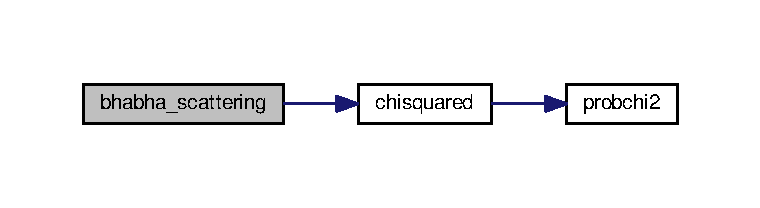
\includegraphics[width=350pt]{_bhabha__fortran__doxy_8f_abb2a1b5ba16400d3f12a537f03a70349_cgraph}
\end{center}
\end{figure}


\index{Bhabha\+\_\+fortran\+\_\+doxy.\+f@{Bhabha\+\_\+fortran\+\_\+doxy.\+f}!chisquared@{chisquared}}
\index{chisquared@{chisquared}!Bhabha\+\_\+fortran\+\_\+doxy.\+f@{Bhabha\+\_\+fortran\+\_\+doxy.\+f}}
\subsubsection[{\texorpdfstring{chisquared(\+N, v, chi, chired, si2)}{chisquared(N, v, chi, chired, si2)}}]{\setlength{\rightskip}{0pt plus 5cm}subroutine chisquared (
\begin{DoxyParamCaption}
\item[{integer}]{N, }
\item[{integer}]{v, }
\item[{double precision}]{chi, }
\item[{double precision}]{chired, }
\item[{double precision}]{si2}
\end{DoxyParamCaption}
)}\hypertarget{_bhabha__fortran__doxy_8f_a45708089271300abc165e88a11ab332e}{}\label{_bhabha__fortran__doxy_8f_a45708089271300abc165e88a11ab332e}
Entrada\+: ~\newline
 ~\newline
 N é o número de pontos no arquivo de dados. ~\newline
 v é o número de variáveis do modelo. ~\newline
 si2 é a energia de centro de massa em GeV. ~\newline
 ~\newline
 Saída\+: ~\newline
 chi é o valor do Qui-\/quadrado em uma dada energia de centro de massa. ~\newline
 chired é o Qui-\/quadrado reduzidos. ~\newline
 ~\newline
 Para calcular o Qui-\/quadrado de uma energia de centro de massa diferente de 34.\+8 GeV, altere as colunas de y(\+N)=C(?,N) e d2y(\+N)=sqrt((C(?,N)/s)$\ast$$\ast$2) para os valores experimentais relacioados a outra energia de centro de massa. Lembrando que y(\+N) é o valor da seção de choque diferencial e d2y o erro desta somado em quadratura. 

Definition at line 120 of file Bhabha\+\_\+fortran\+\_\+doxy.\+f.



Here is the call graph for this function\+:\nopagebreak
\begin{figure}[H]
\begin{center}
\leavevmode
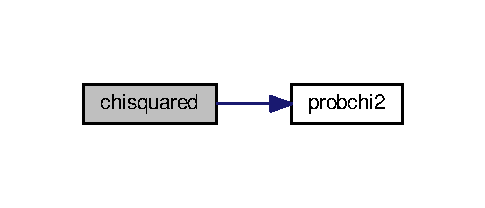
\includegraphics[width=233pt]{_bhabha__fortran__doxy_8f_a45708089271300abc165e88a11ab332e_cgraph}
\end{center}
\end{figure}




Here is the caller graph for this function\+:\nopagebreak
\begin{figure}[H]
\begin{center}
\leavevmode
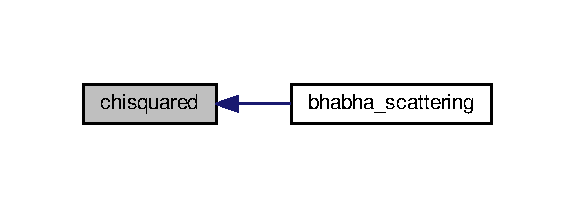
\includegraphics[width=276pt]{_bhabha__fortran__doxy_8f_a45708089271300abc165e88a11ab332e_icgraph}
\end{center}
\end{figure}


\index{Bhabha\+\_\+fortran\+\_\+doxy.\+f@{Bhabha\+\_\+fortran\+\_\+doxy.\+f}!dsigma@{dsigma}}
\index{dsigma@{dsigma}!Bhabha\+\_\+fortran\+\_\+doxy.\+f@{Bhabha\+\_\+fortran\+\_\+doxy.\+f}}
\subsubsection[{\texorpdfstring{dsigma(\+S2, X)}{dsigma(S2, X)}}]{\setlength{\rightskip}{0pt plus 5cm}double precision function dsigma (
\begin{DoxyParamCaption}
\item[{double precision}]{S2, }
\item[{double precision}]{X}
\end{DoxyParamCaption}
)}\hypertarget{_bhabha__fortran__doxy_8f_adb615d7a4a2665478c9f228d3281159e}{}\label{_bhabha__fortran__doxy_8f_adb615d7a4a2665478c9f228d3281159e}


Sessão de choque diferencial \[ \frac{d\sigma}{d\Omega}(S2= \sqrt(s),x = cos(\theta))[\frac{nb}{sterad}] \]. 



Definition at line 61 of file Bhabha\+\_\+fortran\+\_\+doxy.\+f.



Here is the caller graph for this function\+:\nopagebreak
\begin{figure}[H]
\begin{center}
\leavevmode
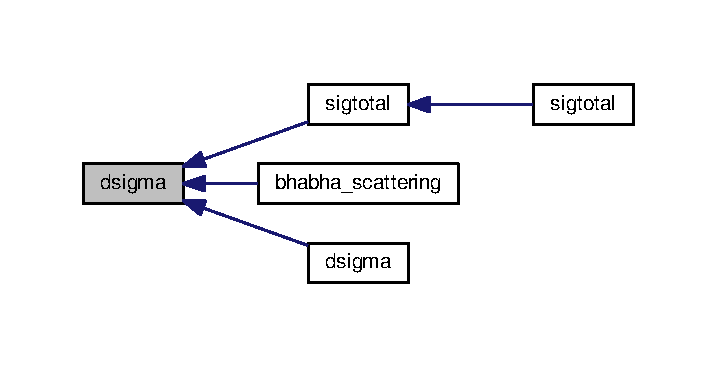
\includegraphics[width=344pt]{_bhabha__fortran__doxy_8f_adb615d7a4a2665478c9f228d3281159e_icgraph}
\end{center}
\end{figure}


\index{Bhabha\+\_\+fortran\+\_\+doxy.\+f@{Bhabha\+\_\+fortran\+\_\+doxy.\+f}!faux@{faux}}
\index{faux@{faux}!Bhabha\+\_\+fortran\+\_\+doxy.\+f@{Bhabha\+\_\+fortran\+\_\+doxy.\+f}}
\subsubsection[{\texorpdfstring{faux(\+X)}{faux(X)}}]{\setlength{\rightskip}{0pt plus 5cm}double precision function faux (
\begin{DoxyParamCaption}
\item[{double precision}]{X}
\end{DoxyParamCaption}
)}\hypertarget{_bhabha__fortran__doxy_8f_a6ccd416a98c419022d77a6fc40b55868}{}\label{_bhabha__fortran__doxy_8f_a6ccd416a98c419022d77a6fc40b55868}


Função auxiliar para a integração da seção de choque diferencial no ângulo sólido. 

\[ \frac{d\sigma}{d\Omega} \cdot 2.0 \ \pi \ \cdot sin(\theta) \] 

Definition at line 88 of file Bhabha\+\_\+fortran\+\_\+doxy.\+f.



Here is the caller graph for this function\+:\nopagebreak
\begin{figure}[H]
\begin{center}
\leavevmode
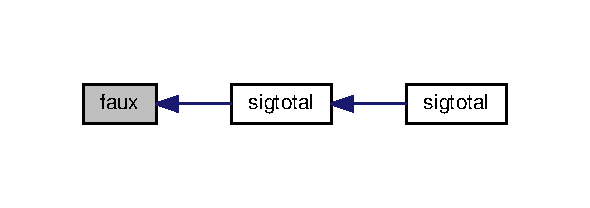
\includegraphics[width=283pt]{_bhabha__fortran__doxy_8f_a6ccd416a98c419022d77a6fc40b55868_icgraph}
\end{center}
\end{figure}


\index{Bhabha\+\_\+fortran\+\_\+doxy.\+f@{Bhabha\+\_\+fortran\+\_\+doxy.\+f}!sigtotal@{sigtotal}}
\index{sigtotal@{sigtotal}!Bhabha\+\_\+fortran\+\_\+doxy.\+f@{Bhabha\+\_\+fortran\+\_\+doxy.\+f}}
\subsubsection[{\texorpdfstring{sigtotal(\+S20)}{sigtotal(S20)}}]{\setlength{\rightskip}{0pt plus 5cm}double precision function sigtotal (
\begin{DoxyParamCaption}
\item[{double precision}]{S20}
\end{DoxyParamCaption}
)}\hypertarget{_bhabha__fortran__doxy_8f_a17b8b02265e091acaccdfb4a9444019f}{}\label{_bhabha__fortran__doxy_8f_a17b8b02265e091acaccdfb4a9444019f}


Seção de choque total \[ \sigma( \ S20 = \sqrt(s) \ ) [nb] \], resultado da integração da função F\+A\+U\+X(\+X) usando a rotina de integração Simpson(função a ser integrada, limite inferior, limite superior, número de intervaloes) 

\[ \sigma[nb] = \int_{-0.84}^{0.84}\! \frac{d\sigma}{d\Omega} \cdot 2.0 \ \pi \ \cdot sin(\theta) \, \mathrm{d}\theta \] 

Definition at line 102 of file Bhabha\+\_\+fortran\+\_\+doxy.\+f.



Here is the call graph for this function\+:\nopagebreak
\begin{figure}[H]
\begin{center}
\leavevmode
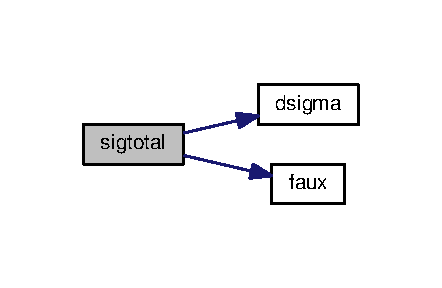
\includegraphics[width=212pt]{_bhabha__fortran__doxy_8f_a17b8b02265e091acaccdfb4a9444019f_cgraph}
\end{center}
\end{figure}




Here is the caller graph for this function\+:\nopagebreak
\begin{figure}[H]
\begin{center}
\leavevmode
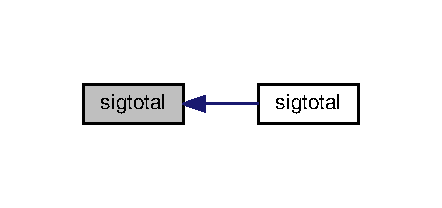
\includegraphics[width=212pt]{_bhabha__fortran__doxy_8f_a17b8b02265e091acaccdfb4a9444019f_icgraph}
\end{center}
\end{figure}



\hypertarget{_bhabha__fortran__sem__doxy_8f}{}\section{Bhabha\+\_\+fortran\+\_\+sem\+\_\+doxy.\+f File Reference}
\label{_bhabha__fortran__sem__doxy_8f}\index{Bhabha\+\_\+fortran\+\_\+sem\+\_\+doxy.\+f@{Bhabha\+\_\+fortran\+\_\+sem\+\_\+doxy.\+f}}
\subsection*{Functions/\+Subroutines}
\begin{DoxyCompactItemize}
\item 
program \hyperlink{_bhabha__fortran__sem__doxy_8f_abb2a1b5ba16400d3f12a537f03a70349}{bhabha\+\_\+scattering}
\item 
double precision function \hyperlink{_bhabha__fortran__sem__doxy_8f_adb615d7a4a2665478c9f228d3281159e}{dsigma} (S2, X)
\item 
double precision function \hyperlink{_bhabha__fortran__sem__doxy_8f_a6ccd416a98c419022d77a6fc40b55868}{faux} (X)
\item 
double precision function \hyperlink{_bhabha__fortran__sem__doxy_8f_a17b8b02265e091acaccdfb4a9444019f}{sigtotal} (S20)
\item 
subroutine \hyperlink{_bhabha__fortran__sem__doxy_8f_a45708089271300abc165e88a11ab332e}{chisquared} (N, v, chi, chired, si2)
\item 
double precision function \hyperlink{_bhabha__fortran__sem__doxy_8f_a2ee8433b8e896ef918c415e17cb0e493}{simpson} (f, a, b, n)
\item 
subroutine \hyperlink{_bhabha__fortran__sem__doxy_8f_a74f0d3f55816e1b65f581a43349f89ba}{probchi2} (x, ndf)
\item 
subroutine \hyperlink{_bhabha__fortran__sem__doxy_8f_ae6b2a5c8e81763258a2b02d8ed0f4bc9}{angle\+\_\+cdf} (x, n, cdf)
\item 
subroutine \hyperlink{_bhabha__fortran__sem__doxy_8f_a83d4ecc8f5a46cbc25cac2fb7937bd44}{angle\+\_\+mean} (n, mean)
\item 
subroutine \hyperlink{_bhabha__fortran__sem__doxy_8f_aea97ae5ed563aa63a80df4f38d19e289}{angle\+\_\+pdf} (x, n, pdf)
\item 
subroutine \hyperlink{_bhabha__fortran__sem__doxy_8f_ae6f220f29d92fd5e4ac84c22029dcbc5}{anglit\+\_\+cdf} (x, cdf)
\item 
subroutine \hyperlink{_bhabha__fortran__sem__doxy_8f_aac69fb6d192dd21c8a01a0b768047f59}{anglit\+\_\+cdf\+\_\+inv} (cdf, x)
\item 
subroutine \hyperlink{_bhabha__fortran__sem__doxy_8f_aedd5857199140786c9bc4b031062c55e}{anglit\+\_\+mean} (mean)
\item 
subroutine \hyperlink{_bhabha__fortran__sem__doxy_8f_a6ac310db648e48aed924a16a04c1ba4e}{anglit\+\_\+pdf} (x, pdf)
\item 
subroutine \hyperlink{_bhabha__fortran__sem__doxy_8f_ad8650a8f15bfee60252281a20c85516e}{anglit\+\_\+sample} (seed, x)
\item 
subroutine \hyperlink{_bhabha__fortran__sem__doxy_8f_a4e147e31b56df3c9c2751b91de61ba28}{anglit\+\_\+variance} (variance)
\item 
subroutine \hyperlink{_bhabha__fortran__sem__doxy_8f_ad1ea95ee407eec1875a81feb0d44d6e1}{arcsin\+\_\+cdf} (x, a, cdf)
\item 
subroutine \hyperlink{_bhabha__fortran__sem__doxy_8f_aeba9ed4e4b270a2c19780190aaaed016}{arcsin\+\_\+cdf\+\_\+inv} (cdf, a, x)
\item 
logical function \hyperlink{_bhabha__fortran__sem__doxy_8f_a6106c25a912dbdfd3a3016548132640e}{arcsin\+\_\+check} (a)
\item 
subroutine \hyperlink{_bhabha__fortran__sem__doxy_8f_a0f3f6a9d53c5ee489f35b5aedd71c3e9}{arcsin\+\_\+mean} (a, mean)
\item 
subroutine \hyperlink{_bhabha__fortran__sem__doxy_8f_a370461195a0a6dbc81d1694f1c900521}{arcsin\+\_\+pdf} (x, a, pdf)
\item 
subroutine \hyperlink{_bhabha__fortran__sem__doxy_8f_af45217dbb90ff9bd690d7d87061616a9}{arcsin\+\_\+sample} (a, seed, x)
\item 
subroutine \hyperlink{_bhabha__fortran__sem__doxy_8f_aec7db221e74872bf1e854e0bd9bab771}{arcsin\+\_\+variance} (a, variance)
\item 
subroutine \hyperlink{_bhabha__fortran__sem__doxy_8f_a9fef702e6bf364a5f85533ca613a7d94}{benford\+\_\+pdf} (x, pdf)
\item 
subroutine \hyperlink{_bhabha__fortran__sem__doxy_8f_a2ef757fb4d120a7339e7ba2d6e4df537}{birthday\+\_\+cdf} (n, cdf)
\item 
subroutine \hyperlink{_bhabha__fortran__sem__doxy_8f_a8688523c630741866353afc455c7a5ee}{birthday\+\_\+cdf\+\_\+inv} (cdf, n)
\item 
subroutine \hyperlink{_bhabha__fortran__sem__doxy_8f_acae6886b34ec452abc19475c7905366b}{birthday\+\_\+pdf} (n, pdf)
\item 
subroutine \hyperlink{_bhabha__fortran__sem__doxy_8f_ab0c099a6932ebc7e4d4378e2bcebfb6a}{bernoulli\+\_\+cdf} (x, a, cdf)
\item 
subroutine \hyperlink{_bhabha__fortran__sem__doxy_8f_aba46047e0d6d0160e9e7f72f468fada8}{bernoulli\+\_\+cdf\+\_\+inv} (cdf, a, x)
\item 
logical function \hyperlink{_bhabha__fortran__sem__doxy_8f_ab60b2073960d9ea664fad920aaccfb29}{bernoulli\+\_\+check} (a)
\item 
subroutine \hyperlink{_bhabha__fortran__sem__doxy_8f_a0b4283a0687fb97d4b5e37594d3d960e}{bernoulli\+\_\+mean} (a, mean)
\item 
subroutine \hyperlink{_bhabha__fortran__sem__doxy_8f_a89fa5f5a4cbaa3ec07e13d430cdbb0b8}{bernoulli\+\_\+pdf} (x, a, pdf)
\item 
subroutine \hyperlink{_bhabha__fortran__sem__doxy_8f_ae46a4cd68c1ca43b8cd6149a3af3451c}{bernoulli\+\_\+sample} (a, seed, x)
\item 
subroutine \hyperlink{_bhabha__fortran__sem__doxy_8f_aac79468ade583fbf0b0faf3fab44bc96}{bernoulli\+\_\+variance} (a, variance)
\item 
double precision function \hyperlink{_bhabha__fortran__sem__doxy_8f_a56f2ab001fb7fd87fd8c17369a866f5a}{bessel\+\_\+i0} (arg)
\item 
subroutine \hyperlink{_bhabha__fortran__sem__doxy_8f_a0508ca5dc920b3b002ac4d769e9e7128}{bessel\+\_\+i0\+\_\+values} (n\+\_\+data, x, fx)
\item 
double precision function, value \hyperlink{_bhabha__fortran__sem__doxy_8f_a4545c4482f31f1e6eddae40f6ed6bbfb}{beta} (a, b)
\item 
subroutine \hyperlink{_bhabha__fortran__sem__doxy_8f_ab79beb1b437d17ea84c53e4d40471f80}{beta\+\_\+binomial\+\_\+cdf} (x, a, b, c, cdf)
\item 
subroutine \hyperlink{_bhabha__fortran__sem__doxy_8f_ae6870b2fc15398bbb52dd3b2ed8c92fb}{beta\+\_\+binomial\+\_\+cdf\+\_\+inv} (cdf, a, b, c, x)
\item 
logical function \hyperlink{_bhabha__fortran__sem__doxy_8f_a35d163e54f3880b3b4a4fc1c46ec6690}{beta\+\_\+binomial\+\_\+check} (a, b, c)
\item 
subroutine \hyperlink{_bhabha__fortran__sem__doxy_8f_af4c24e7e5f9bebb7bde58f72d2d0bef1}{beta\+\_\+binomial\+\_\+mean} (a, b, c, mean)
\item 
subroutine \hyperlink{_bhabha__fortran__sem__doxy_8f_a0b1b4e2bbf9c50969318fac23e17215c}{beta\+\_\+binomial\+\_\+pdf} (x, a, b, c, pdf)
\item 
subroutine \hyperlink{_bhabha__fortran__sem__doxy_8f_ad097654db5e79584fe38d2a53c8ffad8}{beta\+\_\+binomial\+\_\+sample} (a, b, c, seed, x)
\item 
subroutine \hyperlink{_bhabha__fortran__sem__doxy_8f_af18db84101609c96170537b5e09fab18}{beta\+\_\+binomial\+\_\+variance} (a, b, c, variance)
\item 
subroutine \hyperlink{_bhabha__fortran__sem__doxy_8f_a1307bf242705ab2dc0a8db7fc66f4128}{beta\+\_\+cdf} (x, a, b, cdf)
\item 
subroutine \hyperlink{_bhabha__fortran__sem__doxy_8f_ad7b9df743251c691af6f3c722fc44a70}{beta\+\_\+cdf\+\_\+inv} (cdf, p, q, x)
\item 
subroutine \hyperlink{_bhabha__fortran__sem__doxy_8f_a809c02d9b3e29e164a314e6b82989080}{beta\+\_\+cdf\+\_\+inv\+\_\+old} (cdf, a, b, x)
\item 
subroutine \hyperlink{_bhabha__fortran__sem__doxy_8f_a6ca4d09928ee56be09ca34c70fbc37ce}{beta\+\_\+cdf\+\_\+values} (n\+\_\+data, a, b, x, fx)
\item 
logical function \hyperlink{_bhabha__fortran__sem__doxy_8f_a006a8a482ef44095ae5e65425badff73}{beta\+\_\+check} (a, b)
\item 
double precision function \hyperlink{_bhabha__fortran__sem__doxy_8f_a2184970d382ccfa52654d945934a5db9}{beta\+\_\+inc} (a, b, x)
\item 
subroutine \hyperlink{_bhabha__fortran__sem__doxy_8f_ad6f95398deb212fed550fff77fee8aa7}{beta\+\_\+inc\+\_\+values} (n\+\_\+data, a, b, x, fx)
\item 
subroutine \hyperlink{_bhabha__fortran__sem__doxy_8f_a27758be0991a382242cea8fd6d1c6062}{beta\+\_\+mean} (a, b, mean)
\item 
subroutine \hyperlink{_bhabha__fortran__sem__doxy_8f_a98e50467dd638445b02798a39288af88}{beta\+\_\+pdf} (x, a, b, pdf)
\item 
subroutine \hyperlink{_bhabha__fortran__sem__doxy_8f_a4c2f42901cceca59466dde111153a465}{beta\+\_\+sample} (a, b, seed, x)
\item 
subroutine \hyperlink{_bhabha__fortran__sem__doxy_8f_a646b52af6a87a1f9ad45365d12e84074}{beta\+\_\+variance} (a, b, variance)
\item 
subroutine \hyperlink{_bhabha__fortran__sem__doxy_8f_af7299d3fda796eea9a1be0c256f1624b}{binomial\+\_\+cdf} (x, a, b, cdf)
\item 
subroutine \hyperlink{_bhabha__fortran__sem__doxy_8f_a8f4f3c2c05b8593455672a09762700d8}{binomial\+\_\+cdf\+\_\+values} (n\+\_\+data, a, b, x, fx)
\item 
logical function \hyperlink{_bhabha__fortran__sem__doxy_8f_a5a9de1b5360cf06f54e5c25a475a9f34}{geometric\+\_\+check} (a)
\item 
subroutine \hyperlink{_bhabha__fortran__sem__doxy_8f_a1ffa752cfa7e58c775d58ebf3ddff183}{geometric\+\_\+mean} (a, mean)
\item 
subroutine \hyperlink{_bhabha__fortran__sem__doxy_8f_ad7c75816231cf277056551ca6c56d50d}{geometric\+\_\+pdf} (x, a, pdf)
\item 
subroutine \hyperlink{_bhabha__fortran__sem__doxy_8f_a8e9806974aa07e008b7027a4d4fccca8}{geometric\+\_\+sample} (a, seed, x)
\item 
subroutine \hyperlink{_bhabha__fortran__sem__doxy_8f_ae112b39e2f8d5468f1f366cc8e3afd90}{geometric\+\_\+variance} (a, variance)
\item 
subroutine \hyperlink{_bhabha__fortran__sem__doxy_8f_af902e014759d310f9104881f90934632}{gompertz\+\_\+cdf} (x, a, b, cdf)
\item 
subroutine \hyperlink{_bhabha__fortran__sem__doxy_8f_aca5ab8f72105aabb509bd487e8c8b6e6}{gompertz\+\_\+cdf\+\_\+inv} (cdf, a, b, x)
\item 
logical function \hyperlink{_bhabha__fortran__sem__doxy_8f_a6dcecb2ef74b499aa1313117cb5bf666}{gompertz\+\_\+check} (a, b)
\item 
subroutine \hyperlink{_bhabha__fortran__sem__doxy_8f_ad1b796cd8b7d10dc0096cf2a42b748be}{gompertz\+\_\+pdf} (x, a, b, pdf)
\item 
subroutine \hyperlink{_bhabha__fortran__sem__doxy_8f_adee76c73484194b0ddb1c677c0d03407}{gompertz\+\_\+sample} (a, b, seed, x)
\item 
subroutine \hyperlink{_bhabha__fortran__sem__doxy_8f_a3406fe8568d2dfb52a66cc4470893365}{gumbel\+\_\+cdf} (x, cdf)
\item 
subroutine \hyperlink{_bhabha__fortran__sem__doxy_8f_af645551cd94f4f929966f33fade3bb03}{gumbel\+\_\+cdf\+\_\+inv} (cdf, x)
\item 
subroutine \hyperlink{_bhabha__fortran__sem__doxy_8f_ab25784871afe33475733991e2db8c754}{gumbel\+\_\+mean} (mean)
\item 
subroutine \hyperlink{_bhabha__fortran__sem__doxy_8f_a6d2003af12b56d5f9b0a816e24b5775c}{gumbel\+\_\+pdf} (x, pdf)
\item 
subroutine \hyperlink{_bhabha__fortran__sem__doxy_8f_a4eda1bafea5a35dad5e4d1f3c7c4c2fd}{gumbel\+\_\+sample} (seed, x)
\item 
subroutine \hyperlink{_bhabha__fortran__sem__doxy_8f_a0b9d97396f3f7a256ac7b587d8bf44d0}{gumbel\+\_\+variance} (variance)
\item 
subroutine \hyperlink{_bhabha__fortran__sem__doxy_8f_a151eb67716499cd4c2674750d365bbda}{half\+\_\+normal\+\_\+cdf} (x, a, b, cdf)
\item 
subroutine \hyperlink{_bhabha__fortran__sem__doxy_8f_ab3ab8dee9a6bab9e5f838055b6a15e32}{half\+\_\+normal\+\_\+cdf\+\_\+inv} (cdf, a, b, x)
\item 
logical function \hyperlink{_bhabha__fortran__sem__doxy_8f_aff12e14edd4bf669955f0a594154edf8}{half\+\_\+normal\+\_\+check} (a, b)
\item 
subroutine \hyperlink{_bhabha__fortran__sem__doxy_8f_a113c46e78879c405f2eac9a5ffc6df15}{half\+\_\+normal\+\_\+mean} (a, b, mean)
\item 
subroutine \hyperlink{_bhabha__fortran__sem__doxy_8f_ac348bef959fa6ccdecc97def06ad18e3}{half\+\_\+normal\+\_\+pdf} (x, a, b, pdf)
\item 
subroutine \hyperlink{_bhabha__fortran__sem__doxy_8f_ac04ea3c647fa31eab3b163f78f98e75b}{half\+\_\+normal\+\_\+sample} (a, b, seed, x)
\item 
subroutine \hyperlink{_bhabha__fortran__sem__doxy_8f_a3736473676f16f37ee61f098b0d84ab0}{half\+\_\+normal\+\_\+variance} (a, b, variance)
\item 
subroutine \hyperlink{_bhabha__fortran__sem__doxy_8f_af1aca52a5977f25a6cb499968b784a17}{hypergeometric\+\_\+cdf} (x, n, m, l, cdf)
\item 
subroutine \hyperlink{_bhabha__fortran__sem__doxy_8f_a6ebfe3df3fb5de745d4262003a563ca2}{hypergeometric\+\_\+cdf\+\_\+values} (n\+\_\+data, sam, suc, pop,
\item 
logical function \hyperlink{_bhabha__fortran__sem__doxy_8f_a904e056ded5ca1c2d426f58301050514}{log\+\_\+series\+\_\+check} (a)
\item 
subroutine \hyperlink{_bhabha__fortran__sem__doxy_8f_a3f4273816a7b8ae63fa685d5eb79e2b8}{log\+\_\+series\+\_\+mean} (a, mean)
\item 
subroutine \hyperlink{_bhabha__fortran__sem__doxy_8f_a1953093828435ce6e81bbe4921d20c77}{log\+\_\+series\+\_\+pdf} (x, a, pdf)
\item 
subroutine \hyperlink{_bhabha__fortran__sem__doxy_8f_acf82272a3993849e408a1b4ef2143c73}{log\+\_\+series\+\_\+sample} (a, seed, x)
\item 
subroutine \hyperlink{_bhabha__fortran__sem__doxy_8f_ac3ab3c963d117a0ca318fa9e93c94269}{log\+\_\+series\+\_\+variance} (a, variance)
\item 
subroutine \hyperlink{_bhabha__fortran__sem__doxy_8f_adf657f01da631a8c9b66c18577cf36d0}{log\+\_\+uniform\+\_\+cdf} (x, a, b, cdf)
\item 
subroutine \hyperlink{_bhabha__fortran__sem__doxy_8f_af932827c125bbf033c8f22fb759fb08d}{log\+\_\+uniform\+\_\+cdf\+\_\+inv} (cdf, a, b, x)
\item 
logical function \hyperlink{_bhabha__fortran__sem__doxy_8f_ac8db4920c6abba6ea655fdc986813e62}{log\+\_\+uniform\+\_\+check} (a, b)
\item 
subroutine \hyperlink{_bhabha__fortran__sem__doxy_8f_a87623ea0ca476d299aefc8ad2fe08737}{log\+\_\+uniform\+\_\+mean} (a, b, mean)
\item 
subroutine \hyperlink{_bhabha__fortran__sem__doxy_8f_a2e6d975a71a9e29048cc71f0f1c34702}{log\+\_\+uniform\+\_\+pdf} (x, a, b, pdf)
\item 
subroutine \hyperlink{_bhabha__fortran__sem__doxy_8f_af90ae492b3515c794d1306f8ccf26c05}{log\+\_\+uniform\+\_\+sample} (a, b, seed, x)
\item 
subroutine \hyperlink{_bhabha__fortran__sem__doxy_8f_a2d42ac4119c6b4409d419ed9e81a03a0}{lorentz\+\_\+cdf} (x, cdf)
\item 
subroutine \hyperlink{_bhabha__fortran__sem__doxy_8f_a84e9578341d986571a9a7c3aeb2686cc}{lorentz\+\_\+cdf\+\_\+inv} (cdf, x)
\item 
subroutine \hyperlink{_bhabha__fortran__sem__doxy_8f_ad35ecd2cd051d54d3d353c19535da898}{lorentz\+\_\+mean} (mean)
\item 
subroutine \hyperlink{_bhabha__fortran__sem__doxy_8f_aea9281c529fa599fe1103e8d74d33ddc}{lorentz\+\_\+pdf} (x, pdf)
\item 
logical function \hyperlink{_bhabha__fortran__sem__doxy_8f_a564cd13e2df2d52e551d88aa36765b6a}{maxwell\+\_\+check} (a)
\item 
subroutine \hyperlink{_bhabha__fortran__sem__doxy_8f_a3f296baf8d60383b265a902b92a27492}{maxwell\+\_\+mean} (a, mean)
\item 
subroutine \hyperlink{_bhabha__fortran__sem__doxy_8f_aa5b48a50fd2163385ad84b879e0721ef}{maxwell\+\_\+pdf} (x, a, pdf)
\item 
subroutine \hyperlink{_bhabha__fortran__sem__doxy_8f_a288b473fa5808b049b36853ca23b9285}{maxwell\+\_\+sample} (a, seed, x)
\item 
subroutine \hyperlink{_bhabha__fortran__sem__doxy_8f_abd87aa98d26597779513c64c2fbe17e5}{maxwell\+\_\+variance} (a, variance)
\item 
logical function \hyperlink{_bhabha__fortran__sem__doxy_8f_a7119e53d608affd356f7026eef9d2c6b}{multicoef\+\_\+check} (nfactor, factor)
\item 
subroutine \hyperlink{_bhabha__fortran__sem__doxy_8f_a46d0e2c4bd77aa17906a0c078644ef70}{multinomial\+\_\+coef1} (nfactor, factor, ncomb)
\item 
subroutine \hyperlink{_bhabha__fortran__sem__doxy_8f_af3777109b98aa6fc4f03f4addf3aa25a}{multinomial\+\_\+coef2} (nfactor, factor, ncomb)
\item 
logical function \hyperlink{_bhabha__fortran__sem__doxy_8f_a08d328387eca875e6e4607272e11686d}{multinomial\+\_\+check} (a, b, c)
\item 
subroutine \hyperlink{_bhabha__fortran__sem__doxy_8f_a2b11f65f62b24b99045c300950f4339f}{multinomial\+\_\+covariance} (a, b, c, covariance)
\item 
subroutine \hyperlink{_bhabha__fortran__sem__doxy_8f_a57b18d442553cc6c6246577d0d12c251}{multinomial\+\_\+mean} (a, b, c, mean)
\item 
subroutine \hyperlink{_bhabha__fortran__sem__doxy_8f_ac791e27becddd5cfe53d1062d309de3e}{multinomial\+\_\+pdf} (x, a, b, c, pdf)
\item 
subroutine \hyperlink{_bhabha__fortran__sem__doxy_8f_ac6f2948192704b125520724b222c4b17}{multinomial\+\_\+variance} (a, b, c, variance)
\item 
subroutine \hyperlink{_bhabha__fortran__sem__doxy_8f_a43438adca45037973084c5532ff74f9c}{multivariate\+\_\+normal\+\_\+sample} (n, mean, covar\+\_\+factor, see
\item 
subroutine \hyperlink{_bhabha__fortran__sem__doxy_8f_a7d1c9c829d46e6a08ac16ecdcd892ba2}{nakagami\+\_\+cdf} (x, a, b, c, cdf)
\item 
logical function \hyperlink{_bhabha__fortran__sem__doxy_8f_a0fc1a001333a912cdbb380678a85684f}{nakagami\+\_\+check} (a, b, c)
\item 
subroutine \hyperlink{_bhabha__fortran__sem__doxy_8f_af6cbe23e0a51a71de05f4203757b4191}{nakagami\+\_\+mean} (a, b, c, mean)
\item 
subroutine \hyperlink{_bhabha__fortran__sem__doxy_8f_ac2b735b8833a1f49afea86005e5195a8}{nakagami\+\_\+pdf} (x, a, b, c, pdf)
\item 
subroutine \hyperlink{_bhabha__fortran__sem__doxy_8f_a3aa3d66f708fc79f64059739e68629c5}{nakagami\+\_\+variance} (a, b, c, variance)
\item 
subroutine \hyperlink{_bhabha__fortran__sem__doxy_8f_ad671c9a9b8c8f32ec2e8127553c61871}{negative\+\_\+binomial\+\_\+cdf} (x, a, b, cdf)
\item 
subroutine \hyperlink{_bhabha__fortran__sem__doxy_8f_ae12eccbe6c772587d80a92ff74f1d15e}{negative\+\_\+binomial\+\_\+cdf\+\_\+inv} (cdf, a, b, x)
\item 
subroutine \hyperlink{_bhabha__fortran__sem__doxy_8f_ae188cd5921ebcfa4e2b83130bba6f0e7}{negative\+\_\+binomial\+\_\+cdf\+\_\+values} (n\+\_\+data, f, s, p, cdf)
\item 
subroutine \hyperlink{_bhabha__fortran__sem__doxy_8f_a006ebeb017e4f7eca24310e7d1d48ba6}{poisson\+\_\+cdf\+\_\+inv} (cdf, a, x)
\item 
logical function \hyperlink{_bhabha__fortran__sem__doxy_8f_ad5ff3a0c4c674bc96d6540e52c714551}{poisson\+\_\+check} (a)
\item 
subroutine \hyperlink{_bhabha__fortran__sem__doxy_8f_ad3501e0bdf09db56d382eeecdadc4527}{poisson\+\_\+mean} (a, mean)
\item 
subroutine \hyperlink{_bhabha__fortran__sem__doxy_8f_a98a27535cff1de1b8e0031ccb5821e5e}{poisson\+\_\+kernel} (r, n, c, x, y, p)
\item 
subroutine \hyperlink{_bhabha__fortran__sem__doxy_8f_af198c42c12a15059e2968d68eb27f389}{poisson\+\_\+pdf} (x, a, pdf)
\item 
subroutine \hyperlink{_bhabha__fortran__sem__doxy_8f_a7f8c43ba4d755c5e82a3559388c2cae9}{poisson\+\_\+sample} (a, seed, x)
\item 
subroutine \hyperlink{_bhabha__fortran__sem__doxy_8f_a33ab451e2813c47185e508089a51228d}{poisson\+\_\+variance} (a, variance)
\item 
subroutine \hyperlink{_bhabha__fortran__sem__doxy_8f_a80622de6b501cb3b7d068a80cb6ac064}{power\+\_\+cdf} (x, a, b, cdf)
\item 
subroutine \hyperlink{_bhabha__fortran__sem__doxy_8f_adc62d8b1d04a836c565406f798dbe564}{power\+\_\+cdf\+\_\+inv} (cdf, a, b, x)
\item 
logical function \hyperlink{_bhabha__fortran__sem__doxy_8f_a1b88b795db7eec8313c8f3fcf0e332e7}{power\+\_\+check} (a, b)
\item 
subroutine \hyperlink{_bhabha__fortran__sem__doxy_8f_aae67147542b531add7881395ab9b9aa5}{power\+\_\+mean} (a, b, mean)
\item 
subroutine \hyperlink{_bhabha__fortran__sem__doxy_8f_a001ee6b823fa4d4c5bc5c8f0a7e92bc4}{power\+\_\+pdf} (x, a, b, pdf)
\item 
subroutine \hyperlink{_bhabha__fortran__sem__doxy_8f_aade9130fea35054838514ae82f0fc6aa}{power\+\_\+sample} (a, b, seed, x)
\item 
subroutine \hyperlink{_bhabha__fortran__sem__doxy_8f_a37db6d376f844e99257c1b319ddbf6b0}{power\+\_\+variance} (a, b, variance)
\item 
subroutine \hyperlink{_bhabha__fortran__sem__doxy_8f_ae149433719bfb4e008585cb535e0a6d9}{psi\+\_\+values} (n\+\_\+data, x, fx)
\item 
subroutine \hyperlink{_bhabha__fortran__sem__doxy_8f_aab048bbbc5041ebb417d263ffe3e72ed}{quasigeometric\+\_\+cdf} (x, a, b, cdf)
\item 
subroutine \hyperlink{_bhabha__fortran__sem__doxy_8f_a810c63c1882371219cad270ca4181c25}{quasigeometric\+\_\+cdf\+\_\+inv} (cdf, a, b, x)
\item 
logical function \hyperlink{_bhabha__fortran__sem__doxy_8f_a96bb9b2b221ea79c95939f9dbe18e9ea}{quasigeometric\+\_\+check} (a, b)
\item 
subroutine \hyperlink{_bhabha__fortran__sem__doxy_8f_a418662fcf5cf28009331bdcfec409cdf}{quasigeometric\+\_\+mean} (a, b, mean)
\item 
subroutine \hyperlink{_bhabha__fortran__sem__doxy_8f_a57411de0fdc63ca7e4e22123a96481fa}{quasigeometric\+\_\+pdf} (x, a, b, pdf)
\item 
subroutine \hyperlink{_bhabha__fortran__sem__doxy_8f_a1256bc0c59e7792531846e68107508c0}{quasigeometric\+\_\+sample} (a, b, seed, x)
\item 
subroutine \hyperlink{_bhabha__fortran__sem__doxy_8f_a8a8ee18a7af38d1039a568f9addd8f82}{quasigeometric\+\_\+variance} (a, b, variance)
\item 
real function \hyperlink{_bhabha__fortran__sem__doxy_8f_ae3ff5bb6289eaf322c0388b7b4bef196}{r4\+\_\+uniform\+\_\+ab} (a, b, seed)
\item 
function \hyperlink{_bhabha__fortran__sem__doxy_8f_ad22a9ea3f2620ff201ba0eeec82e0ae6}{r4\+\_\+uniform\+\_\+01} (seed)
\item 
function \hyperlink{_bhabha__fortran__sem__doxy_8f_ac9af998845bffd8c6eed4d4cf52d9c08}{r8\+\_\+epsilon} ()
\item 
function \hyperlink{_bhabha__fortran__sem__doxy_8f_adda13d639fe87cc3f3c9875a30c8276c}{r8\+\_\+uniform\+\_\+01} (seed)
\item 
subroutine \hyperlink{_bhabha__fortran__sem__doxy_8f_acd023da27fb88ef28004cf11f5942d05}{r8mat\+\_\+print} (m, n, a, title)
\item 
subroutine \hyperlink{_bhabha__fortran__sem__doxy_8f_a432586d1ce42c3c748dc0659c9626c86}{r8mat\+\_\+print\+\_\+some} (m, n, a, ilo, jlo, ihi, jhi,
\item 
subroutine \hyperlink{_bhabha__fortran__sem__doxy_8f_a704f15e9fc2805ec7c3daf97bb353f1c}{r8row\+\_\+max} (m, n, a, amax)
\item 
subroutine \hyperlink{_bhabha__fortran__sem__doxy_8f_a0d5ecf067cee9f1578dbce581a7eccf4}{r8row\+\_\+mean} (m, n, a, mean)
\item 
subroutine \hyperlink{_bhabha__fortran__sem__doxy_8f_a7c1325ae8ea9f6aa9109e208712afcd1}{r8row\+\_\+min} (m, n, a, amin)
\item 
subroutine \hyperlink{_bhabha__fortran__sem__doxy_8f_a3a87c9f6e18e8c777449225e06a1124e}{r8row\+\_\+variance} (m, n, a, variance)
\item 
subroutine \hyperlink{_bhabha__fortran__sem__doxy_8f_a6f5548af22c5933a7360db1eefaa985e}{r8vec\+\_\+circular\+\_\+variance} (n, x, circular\+\_\+variance)
\item 
function \hyperlink{_bhabha__fortran__sem__doxy_8f_a53818831efeb1c9cea9cda383bdfebf1}{r8vec\+\_\+dot\+\_\+product} (n, v1, v2)
\item 
subroutine \hyperlink{_bhabha__fortran__sem__doxy_8f_a3afb0bc60d390433659934e42be314b5}{r8vec\+\_\+mean} (n, x, mean)
\item 
subroutine \hyperlink{_bhabha__fortran__sem__doxy_8f_a5068c55b384e4d8de2b97c2ac9fb9f23}{r8vec\+\_\+min} (n, a, amin)
\item 
subroutine \hyperlink{_bhabha__fortran__sem__doxy_8f_a34c59b6daeb8820b723412d8d9bdf687}{r8vec\+\_\+uniform\+\_\+ab} (n, a, b, seed, r)
\item 
subroutine \hyperlink{_bhabha__fortran__sem__doxy_8f_a5e64b19c036489d0c15f5a2c7ba0e216}{r8vec\+\_\+uniform\+\_\+01} (n, seed, r)
\item 
subroutine \hyperlink{_bhabha__fortran__sem__doxy_8f_aca8f7af53e9c8384405cbe2eecf3deb0}{r8vec\+\_\+unit\+\_\+sum} (n, a)
\item 
subroutine \hyperlink{_bhabha__fortran__sem__doxy_8f_aeac2d8faada0a83b125ddbaa53060f71}{r8vec\+\_\+variance} (n, x, variance)
\item 
subroutine \hyperlink{_bhabha__fortran__sem__doxy_8f_aaa2c63bb728acee27317c0481a5bdbdb}{rayleigh\+\_\+cdf} (x, a, cdf)
\item 
subroutine \hyperlink{_bhabha__fortran__sem__doxy_8f_a6cb29161b358879878553289cb675d94}{rayleigh\+\_\+cdf\+\_\+inv} (cdf, a, x)
\item 
subroutine \hyperlink{_bhabha__fortran__sem__doxy_8f_a638657c28d62e70530a378d9a2920ee2}{rayleigh\+\_\+cdf\+\_\+values} (n\+\_\+data, sigma, x, fx)
\item 
logical function \hyperlink{_bhabha__fortran__sem__doxy_8f_a636b798611edb695a18fcc189bbcfa8b}{rayleigh\+\_\+check} (a)
\item 
subroutine \hyperlink{_bhabha__fortran__sem__doxy_8f_a1913ce88098196a93906c3294a213a42}{rayleigh\+\_\+mean} (a, mean)
\item 
subroutine \hyperlink{_bhabha__fortran__sem__doxy_8f_aed2225b609bc0484d8a878d661ca06f5}{rayleigh\+\_\+pdf} (x, a, pdf)
\item 
subroutine \hyperlink{_bhabha__fortran__sem__doxy_8f_a37c29cebf26c80f5eca6d552281f6e4c}{rayleigh\+\_\+sample} (a, seed, x)
\item 
subroutine \hyperlink{_bhabha__fortran__sem__doxy_8f_a70e2c28fcfac69b8f4a5df3f1472fa15}{rayleigh\+\_\+variance} (a, variance)
\item 
subroutine \hyperlink{_bhabha__fortran__sem__doxy_8f_ae28b3530dc8de971f919080de1b93e80}{reciprocal\+\_\+cdf} (x, a, b, cdf)
\item 
subroutine \hyperlink{_bhabha__fortran__sem__doxy_8f_aa0605b5b606ef51bd36ef48ce4919924}{reciprocal\+\_\+cdf\+\_\+inv} (cdf, a, b, x)
\item 
logical function \hyperlink{_bhabha__fortran__sem__doxy_8f_af51dabb725b02ab97b328de46978219f}{reciprocal\+\_\+check} (a, b)
\item 
subroutine \hyperlink{_bhabha__fortran__sem__doxy_8f_ac0440a31997ff53e6f93ce9ee20af3ec}{reciprocal\+\_\+mean} (a, b, mean)
\item 
subroutine \hyperlink{_bhabha__fortran__sem__doxy_8f_a450f3e05aa915649721ddf2d61bf47fa}{reciprocal\+\_\+pdf} (x, a, b, pdf)
\item 
subroutine \hyperlink{_bhabha__fortran__sem__doxy_8f_abdaf248fa3bc68293411d44d881e2865}{reciprocal\+\_\+sample} (a, b, seed, x)
\item 
subroutine \hyperlink{_bhabha__fortran__sem__doxy_8f_a3c7e3917a239f43779f620c2e5863720}{reciprocal\+\_\+variance} (a, b, variance)
\item 
subroutine \hyperlink{_bhabha__fortran__sem__doxy_8f_a7388ce0c1e1baabe68d488afdddf9f76}{ribesl} (x, alpha, nb, ize, b, ncalc)
\item 
subroutine \hyperlink{_bhabha__fortran__sem__doxy_8f_a547f8f40db56f1abdf6d11537ff1ac85}{runs\+\_\+sample} (m, n, seed, r)
\item 
subroutine \hyperlink{_bhabha__fortran__sem__doxy_8f_a84945493088e8f98d15cf401c100e82c}{runs\+\_\+simulate} (m, n, seed, a)
\item 
subroutine \hyperlink{_bhabha__fortran__sem__doxy_8f_aa77c037b8f90a49ff7a1d9f4dde58aeb}{runs\+\_\+variance} (m, n, variance)
\item 
double precision function \hyperlink{_bhabha__fortran__sem__doxy_8f_a1749f7d18d74526e8948745e077f05d6}{sech} (x)
\item 
subroutine \hyperlink{_bhabha__fortran__sem__doxy_8f_ac322fce1f5c0595f018644a3a250015d}{sech\+\_\+cdf} (x, a, b, cdf)
\item 
subroutine \hyperlink{_bhabha__fortran__sem__doxy_8f_a48c395063f1fe4584b741fd7b8c20ca3}{sech\+\_\+cdf\+\_\+inv} (cdf, a, b, x)
\item 
logical function \hyperlink{_bhabha__fortran__sem__doxy_8f_aaa8b88a5a18965765dd105f35f27334e}{sech\+\_\+check} (a, b)
\item 
subroutine \hyperlink{_bhabha__fortran__sem__doxy_8f_a3883c0db4be7be699a5beeed32adb504}{sech\+\_\+mean} (a, b, mean)
\item 
subroutine \hyperlink{_bhabha__fortran__sem__doxy_8f_a688a7b361741dad3d269d8081b912f76}{sech\+\_\+pdf} (x, a, b, pdf)
\item 
subroutine \hyperlink{_bhabha__fortran__sem__doxy_8f_a3b87004baabafee7ad7ec925d02fbffa}{sech\+\_\+sample} (a, b, seed, x)
\item 
subroutine \hyperlink{_bhabha__fortran__sem__doxy_8f_a2520eac72066583e24fc121018b6ba2e}{sech\+\_\+variance} (a, b, variance)
\item 
subroutine \hyperlink{_bhabha__fortran__sem__doxy_8f_a4bd980f50e41d09ed86abca21d3dfa14}{semicircular\+\_\+cdf} (x, a, b, cdf)
\item 
subroutine \hyperlink{_bhabha__fortran__sem__doxy_8f_a6d0ee2a8130e550cd689cd255ccc60cc}{semicircular\+\_\+cdf\+\_\+inv} (cdf, a, b, x)
\item 
logical function \hyperlink{_bhabha__fortran__sem__doxy_8f_a7190d7f0fbac6430ec693e54dc1aa636}{semicircular\+\_\+check} (a, b)
\item 
subroutine \hyperlink{_bhabha__fortran__sem__doxy_8f_ad13798246f26b503c71d03dc1397d510}{semicircular\+\_\+mean} (a, b, mean)
\item 
subroutine \hyperlink{_bhabha__fortran__sem__doxy_8f_a9f8895094b6821e14853bae849297fca}{semicircular\+\_\+pdf} (x, a, b, pdf)
\item 
subroutine \hyperlink{_bhabha__fortran__sem__doxy_8f_ab458959d3e85a81b418a1e703fda7ce7}{semicircular\+\_\+sample} (a, b, seed, x)
\item 
subroutine \hyperlink{_bhabha__fortran__sem__doxy_8f_a01f045ae1d9d3cb85e0de3e1d207f5f9}{semicircular\+\_\+variance} (a, b, variance)
\item 
double precision function \hyperlink{_bhabha__fortran__sem__doxy_8f_a11b103a7500f33e4679f27dcc250d7eb}{sin\+\_\+power\+\_\+int} (a, b, n)
\item 
double precision function \hyperlink{_bhabha__fortran__sem__doxy_8f_aaa5d69bd35accf7257e983f76d12cb87}{sphere\+\_\+unit\+\_\+area\+\_\+nd} (dim\+\_\+num)
\item 
integer function \hyperlink{_bhabha__fortran__sem__doxy_8f_a917c5cb6942b4f683a70b827c88476bd}{stirling2\+\_\+value} (n, m)
\item 
subroutine \hyperlink{_bhabha__fortran__sem__doxy_8f_a4b8711966343cd70dc9ead18b8252ad1}{student\+\_\+cdf} (x, a, b, c, cdf)
\item 
subroutine \hyperlink{_bhabha__fortran__sem__doxy_8f_a20e37e60ef6e1d53450d1096d6179ae2}{student\+\_\+cdf\+\_\+values} (n\+\_\+data, c, x, fx)
\item 
logical function \hyperlink{_bhabha__fortran__sem__doxy_8f_a33e0ec77dcaf5ed332a05ab10b34af0c}{student\+\_\+check} (a, b, c)
\item 
subroutine \hyperlink{_bhabha__fortran__sem__doxy_8f_adef794feac6716fffa86207bf008f854}{student\+\_\+mean} (a, b, c, mean)
\item 
subroutine \hyperlink{_bhabha__fortran__sem__doxy_8f_ad0cdf2c699e02784d889de817e73db3a}{student\+\_\+pdf} (x, a, b, c, pdf)
\item 
subroutine \hyperlink{_bhabha__fortran__sem__doxy_8f_a704ccb9e1dc4d1755ebb37a50d5687de}{student\+\_\+sample} (a, b, c, seed, x)
\item 
subroutine \hyperlink{_bhabha__fortran__sem__doxy_8f_a5fda95cb2ebc1ee3712f6b0d07243c22}{student\+\_\+variance} (a, b, c, variance)
\item 
subroutine \hyperlink{_bhabha__fortran__sem__doxy_8f_a4e75238f2d952890a3b1999e87d07d77}{student\+\_\+noncentral\+\_\+cdf} (x, idf, d, cdf)
\item 
subroutine \hyperlink{_bhabha__fortran__sem__doxy_8f_a7af277756a7246db9ab5286f0a03010a}{student\+\_\+noncentral\+\_\+cdf\+\_\+values} (n\+\_\+data, df, lambda,
\item 
function \hyperlink{_bhabha__fortran__sem__doxy_8f_ab24bd8b58c02c63b5053a52f6fdb8be6}{tfn} (h, a)
\item 
logical function \hyperlink{_bhabha__fortran__sem__doxy_8f_ac17f060df4ddff505ffdf4fd42f83da3}{triangle\+\_\+check} (a, b, c)
\item 
subroutine \hyperlink{_bhabha__fortran__sem__doxy_8f_a3220ee5b701d76c400b43ab093c03f16}{triangle\+\_\+mean} (a, b, c, mean)
\item 
subroutine \hyperlink{_bhabha__fortran__sem__doxy_8f_aae66d0c6853e05e39d4730371449a711}{triangle\+\_\+pdf} (x, a, b, c, pdf)
\item 
subroutine \hyperlink{_bhabha__fortran__sem__doxy_8f_ad37277b4efa293c44cc27fc4bd981e8f}{triangle\+\_\+sample} (a, b, c, seed, x)
\item 
subroutine \hyperlink{_bhabha__fortran__sem__doxy_8f_abc70f31d109699c1245a87ebc99a5736}{triangle\+\_\+variance} (a, b, c, variance)
\item 
subroutine \hyperlink{_bhabha__fortran__sem__doxy_8f_a829742571d36a8b07342c12ea3112f28}{triangular\+\_\+cdf} (x, a, b, cdf)
\item 
subroutine \hyperlink{_bhabha__fortran__sem__doxy_8f_ab66652c0bf9ae711b9b75cd1e6e251c5}{triangular\+\_\+cdf\+\_\+inv} (cdf, a, b, x)
\item 
logical function \hyperlink{_bhabha__fortran__sem__doxy_8f_a1075d4be52d9e73dc2d16c5e4578d58b}{triangular\+\_\+check} (a, b)
\item 
subroutine \hyperlink{_bhabha__fortran__sem__doxy_8f_aab67668dc75a0d2884868176020040bd}{triangular\+\_\+mean} (a, b, mean)
\item 
subroutine \hyperlink{_bhabha__fortran__sem__doxy_8f_a2ff19917924536f55f55531b148a4d60}{triangular\+\_\+pdf} (x, a, b, pdf)
\item 
subroutine \hyperlink{_bhabha__fortran__sem__doxy_8f_aa6b6114d8735ccfa463f60f4b9c08748}{triangular\+\_\+sample} (a, b, seed, x)
\item 
subroutine \hyperlink{_bhabha__fortran__sem__doxy_8f_a8e94727635c279a064a2c497a9175a04}{triangular\+\_\+variance} (a, b, variance)
\item 
double precision function \hyperlink{_bhabha__fortran__sem__doxy_8f_aa287ba105f62a96aee81e3a9f0b0fc6d}{trigamma} (x)
\item 
subroutine \hyperlink{_bhabha__fortran__sem__doxy_8f_a4542d552be72b2153a3e27324241d9b1}{uniform\+\_\+01\+\_\+cdf} (x, cdf)
\item 
subroutine \hyperlink{_bhabha__fortran__sem__doxy_8f_a72aba79732c10141024277c78076d1c4}{uniform\+\_\+01\+\_\+cdf\+\_\+inv} (cdf, x)
\item 
subroutine \hyperlink{_bhabha__fortran__sem__doxy_8f_a703c0741a0197996b0e9c9341bc0fb20}{uniform\+\_\+01\+\_\+mean} (mean)
\item 
subroutine \hyperlink{_bhabha__fortran__sem__doxy_8f_ac1f3e1cf38a7750036257dd222d4d133}{uniform\+\_\+01\+\_\+order\+\_\+sample} (n, seed, x)
\item 
subroutine \hyperlink{_bhabha__fortran__sem__doxy_8f_a20a976304b1a9dc6e1fbc03e504bc1ef}{uniform\+\_\+01\+\_\+pdf} (x, pdf)
\item 
double precision function \hyperlink{_bhabha__fortran__sem__doxy_8f_a486635f122e7078b243c9f56a9a1e247}{uniform\+\_\+01\+\_\+sample} (seed)
\item 
logical function \hyperlink{_bhabha__fortran__sem__doxy_8f_aa375f84c7dcbc6bd08516cb6c18fcf8a}{uniform\+\_\+check} (a, b)
\item 
subroutine \hyperlink{_bhabha__fortran__sem__doxy_8f_a3073152f6052f105e100e23e980a9dce}{uniform\+\_\+mean} (a, b, mean)
\item 
subroutine \hyperlink{_bhabha__fortran__sem__doxy_8f_a05ec2d1bc3328a8aad5e598852bcbf14}{uniform\+\_\+pdf} (x, a, b, pdf)
\item 
subroutine \hyperlink{_bhabha__fortran__sem__doxy_8f_af92ef0ba8e3c9c529f7b1c4eb0bed4c0}{uniform\+\_\+sample} (a, b, seed, x)
\item 
subroutine \hyperlink{_bhabha__fortran__sem__doxy_8f_a9f30db560b85d07014de26e90a80c834}{uniform\+\_\+variance} (a, b, variance)
\item 
subroutine \hyperlink{_bhabha__fortran__sem__doxy_8f_a70846f32a4c049b18e01802a92db7d96}{uniform\+\_\+discrete\+\_\+cdf} (x, a, b, cdf)
\item 
subroutine \hyperlink{_bhabha__fortran__sem__doxy_8f_aafa76f1cf208f904b15993e0ef66eb85}{uniform\+\_\+discrete\+\_\+cdf\+\_\+inv} (cdf, a, b, x)
\item 
logical function \hyperlink{_bhabha__fortran__sem__doxy_8f_a422da08e6639b40b1e57fac092fde67d}{uniform\+\_\+discrete\+\_\+check} (a, b)
\item 
subroutine \hyperlink{_bhabha__fortran__sem__doxy_8f_a03a4be1295ed7192ae91041a1e64a807}{uniform\+\_\+discrete\+\_\+mean} (a, b, mean)
\item 
subroutine \hyperlink{_bhabha__fortran__sem__doxy_8f_af3de0b9e0c5a479e445bb097f5e6289a}{uniform\+\_\+discrete\+\_\+pdf} (x, a, b, pdf)
\item 
subroutine \hyperlink{_bhabha__fortran__sem__doxy_8f_a224e9cbefb5f1ef40f22420215fd18af}{uniform\+\_\+discrete\+\_\+sample} (a, b, seed, x)
\item 
subroutine \hyperlink{_bhabha__fortran__sem__doxy_8f_a874a7fc75f53b8a682b9c8978939fda5}{uniform\+\_\+discrete\+\_\+variance} (a, b, variance)
\item 
subroutine \hyperlink{_bhabha__fortran__sem__doxy_8f_a567091bcdecad2248c96535c412d6195}{uniform\+\_\+nsphere\+\_\+sample} (n, seed, x)
\item 
subroutine \hyperlink{_bhabha__fortran__sem__doxy_8f_a5c4785e88e38b424c52cce4689445dfc}{von\+\_\+mises\+\_\+cdf} (x, a, b, cdf)
\item 
subroutine \hyperlink{_bhabha__fortran__sem__doxy_8f_a0d6b2b89e87cdefab6293dcb412af08f}{von\+\_\+mises\+\_\+cdf\+\_\+inv} (cdf, a, b, x)
\item 
subroutine \hyperlink{_bhabha__fortran__sem__doxy_8f_a4c65f800f570436a4cb12dddb3c8b7a3}{von\+\_\+mises\+\_\+cdf\+\_\+values} (n\+\_\+data, a, b, x, fx)
\item 
logical function \hyperlink{_bhabha__fortran__sem__doxy_8f_a40a097c025b70be0e09b0de70e1da45b}{von\+\_\+mises\+\_\+check} (a, b)
\item 
subroutine \hyperlink{_bhabha__fortran__sem__doxy_8f_a662131cbe821a341319c8a9ca67f95af}{von\+\_\+mises\+\_\+circular\+\_\+variance} (a, b, circular\+\_\+variance)
\item 
subroutine \hyperlink{_bhabha__fortran__sem__doxy_8f_a97b8b21e59cd05efc755304eb6fd543f}{von\+\_\+mises\+\_\+mean} (a, b, mean)
\item 
subroutine \hyperlink{_bhabha__fortran__sem__doxy_8f_a385af85b16bbe1659e0de9e6e916d3d3}{von\+\_\+mises\+\_\+pdf} (x, a, b, pdf)
\item 
subroutine \hyperlink{_bhabha__fortran__sem__doxy_8f_a06bd71cbe32f074e5bb5ca85524936be}{von\+\_\+mises\+\_\+sample} (a, b, seed, x)
\item 
subroutine \hyperlink{_bhabha__fortran__sem__doxy_8f_ae3e1a96ae8ad17ffd698fba05207d5f8}{weibull\+\_\+cdf} (x, a, b, c, cdf)
\item 
subroutine \hyperlink{_bhabha__fortran__sem__doxy_8f_a017a7f1ff8e2de34d608525f4fa057da}{weibull\+\_\+cdf\+\_\+inv} (cdf, a, b, c, x)
\item 
subroutine \hyperlink{_bhabha__fortran__sem__doxy_8f_aed1852e1d63e6ebf573f1ff0e117f958}{weibull\+\_\+cdf\+\_\+values} (n\+\_\+data, alpha, \hyperlink{_bhabha__fortran__sem__doxy_8f_a4545c4482f31f1e6eddae40f6ed6bbfb}{beta}, x, fx)
\item 
logical function \hyperlink{_bhabha__fortran__sem__doxy_8f_afb02fe9720b1d511216ff02e43dc6b5e}{weibull\+\_\+check} (a, b, c)
\item 
subroutine \hyperlink{_bhabha__fortran__sem__doxy_8f_a023bd1260ec4d716669eca0aa0309343}{weibull\+\_\+mean} (a, b, c, mean)
\item 
subroutine \hyperlink{_bhabha__fortran__sem__doxy_8f_a9f72d60350cbaeb6b488cd822a8b59c3}{weibull\+\_\+pdf} (x, a, b, c, pdf)
\item 
subroutine \hyperlink{_bhabha__fortran__sem__doxy_8f_a9f7c934964fac585c5369f957382eab0}{weibull\+\_\+sample} (a, b, c, seed, x)
\item 
subroutine \hyperlink{_bhabha__fortran__sem__doxy_8f_a5c4e758650cdd5f1f407a932e1cde105}{weibull\+\_\+variance} (a, b, c, variance)
\item 
subroutine \hyperlink{_bhabha__fortran__sem__doxy_8f_ab34b5e8666ea41c5ab564c56a11e88f1}{weibull\+\_\+discrete\+\_\+cdf} (x, a, b, cdf)
\item 
subroutine \hyperlink{_bhabha__fortran__sem__doxy_8f_a1204dfb7e8bc98633fbe31061c370c85}{weibull\+\_\+discrete\+\_\+cdf\+\_\+inv} (cdf, a, b, x)
\item 
logical function \hyperlink{_bhabha__fortran__sem__doxy_8f_aa9fecd5de6c8f01d32d025cde7443dbb}{weibull\+\_\+discrete\+\_\+check} (a, b)
\item 
subroutine \hyperlink{_bhabha__fortran__sem__doxy_8f_a9550bf6e0d0c82862d6c811291ff9a53}{weibull\+\_\+discrete\+\_\+pdf} (x, a, b, pdf)
\item 
subroutine \hyperlink{_bhabha__fortran__sem__doxy_8f_a34a92d791e6c7276adcbe1cd6e9c366f}{weibull\+\_\+discrete\+\_\+sample} (a, b, seed, x)
\item 
double precision function, value \hyperlink{_bhabha__fortran__sem__doxy_8f_a2ad5727389a72db607052fa457bacf7b}{zeta} (p)
\item 
subroutine \hyperlink{_bhabha__fortran__sem__doxy_8f_ae8a401a7b095f2303a3025ec1a6080c1}{zipf\+\_\+cdf} (x, a, cdf)
\item 
logical function \hyperlink{_bhabha__fortran__sem__doxy_8f_aa599fb17c8b01fde08d9683d746266c6}{zipf\+\_\+check} (a)
\item 
subroutine \hyperlink{_bhabha__fortran__sem__doxy_8f_ab3bfbabacbc67bb7feff780328a4a26c}{zipf\+\_\+mean} (a, mean)
\item 
subroutine \hyperlink{_bhabha__fortran__sem__doxy_8f_ac57c48834bf4850b8278bd8af5bac9ad}{zipf\+\_\+pdf} (x, a, pdf)
\item 
subroutine \hyperlink{_bhabha__fortran__sem__doxy_8f_a5098279191de72d2fbd4a7457caaf060}{zipf\+\_\+sample} (a, seed, x)
\item 
subroutine \hyperlink{_bhabha__fortran__sem__doxy_8f_aaa5f46761caed5c5998401d0fbc17c58}{zipf\+\_\+variance} (a, variance)
\end{DoxyCompactItemize}


\subsection{Function/\+Subroutine Documentation}
\index{Bhabha\+\_\+fortran\+\_\+sem\+\_\+doxy.\+f@{Bhabha\+\_\+fortran\+\_\+sem\+\_\+doxy.\+f}!angle\+\_\+cdf@{angle\+\_\+cdf}}
\index{angle\+\_\+cdf@{angle\+\_\+cdf}!Bhabha\+\_\+fortran\+\_\+sem\+\_\+doxy.\+f@{Bhabha\+\_\+fortran\+\_\+sem\+\_\+doxy.\+f}}
\subsubsection[{\texorpdfstring{angle\+\_\+cdf(x, n, cdf)}{angle_cdf(x, n, cdf)}}]{\setlength{\rightskip}{0pt plus 5cm}subroutine angle\+\_\+cdf (
\begin{DoxyParamCaption}
\item[{double precision}]{x, }
\item[{integer}]{n, }
\item[{double precision, value}]{cdf}
\end{DoxyParamCaption}
)}\hypertarget{_bhabha__fortran__sem__doxy_8f_ae6b2a5c8e81763258a2b02d8ed0f4bc9}{}\label{_bhabha__fortran__sem__doxy_8f_ae6b2a5c8e81763258a2b02d8ed0f4bc9}


Definition at line 210 of file Bhabha\+\_\+fortran\+\_\+sem\+\_\+doxy.\+f.



Here is the call graph for this function\+:\nopagebreak
\begin{figure}[H]
\begin{center}
\leavevmode
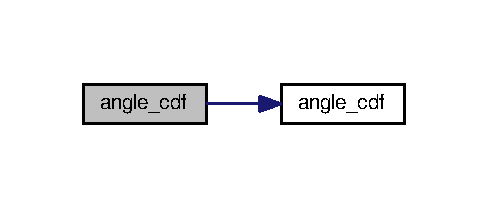
\includegraphics[width=234pt]{_bhabha__fortran__sem__doxy_8f_ae6b2a5c8e81763258a2b02d8ed0f4bc9_cgraph}
\end{center}
\end{figure}


\index{Bhabha\+\_\+fortran\+\_\+sem\+\_\+doxy.\+f@{Bhabha\+\_\+fortran\+\_\+sem\+\_\+doxy.\+f}!angle\+\_\+mean@{angle\+\_\+mean}}
\index{angle\+\_\+mean@{angle\+\_\+mean}!Bhabha\+\_\+fortran\+\_\+sem\+\_\+doxy.\+f@{Bhabha\+\_\+fortran\+\_\+sem\+\_\+doxy.\+f}}
\subsubsection[{\texorpdfstring{angle\+\_\+mean(n, mean)}{angle_mean(n, mean)}}]{\setlength{\rightskip}{0pt plus 5cm}subroutine angle\+\_\+mean (
\begin{DoxyParamCaption}
\item[{integer}]{n, }
\item[{double precision}]{mean}
\end{DoxyParamCaption}
)}\hypertarget{_bhabha__fortran__sem__doxy_8f_a83d4ecc8f5a46cbc25cac2fb7937bd44}{}\label{_bhabha__fortran__sem__doxy_8f_a83d4ecc8f5a46cbc25cac2fb7937bd44}


Definition at line 281 of file Bhabha\+\_\+fortran\+\_\+sem\+\_\+doxy.\+f.



Here is the call graph for this function\+:\nopagebreak
\begin{figure}[H]
\begin{center}
\leavevmode
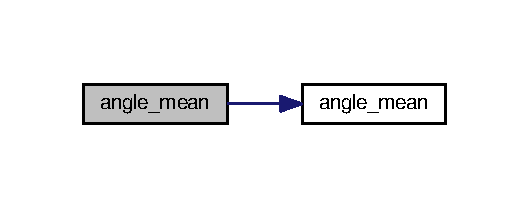
\includegraphics[width=254pt]{_bhabha__fortran__sem__doxy_8f_a83d4ecc8f5a46cbc25cac2fb7937bd44_cgraph}
\end{center}
\end{figure}


\index{Bhabha\+\_\+fortran\+\_\+sem\+\_\+doxy.\+f@{Bhabha\+\_\+fortran\+\_\+sem\+\_\+doxy.\+f}!angle\+\_\+pdf@{angle\+\_\+pdf}}
\index{angle\+\_\+pdf@{angle\+\_\+pdf}!Bhabha\+\_\+fortran\+\_\+sem\+\_\+doxy.\+f@{Bhabha\+\_\+fortran\+\_\+sem\+\_\+doxy.\+f}}
\subsubsection[{\texorpdfstring{angle\+\_\+pdf(x, n, pdf)}{angle_pdf(x, n, pdf)}}]{\setlength{\rightskip}{0pt plus 5cm}subroutine angle\+\_\+pdf (
\begin{DoxyParamCaption}
\item[{double precision}]{x, }
\item[{integer}]{n, }
\item[{double precision, value}]{pdf}
\end{DoxyParamCaption}
)}\hypertarget{_bhabha__fortran__sem__doxy_8f_aea97ae5ed563aa63a80df4f38d19e289}{}\label{_bhabha__fortran__sem__doxy_8f_aea97ae5ed563aa63a80df4f38d19e289}


Definition at line 317 of file Bhabha\+\_\+fortran\+\_\+sem\+\_\+doxy.\+f.



Here is the call graph for this function\+:\nopagebreak
\begin{figure}[H]
\begin{center}
\leavevmode
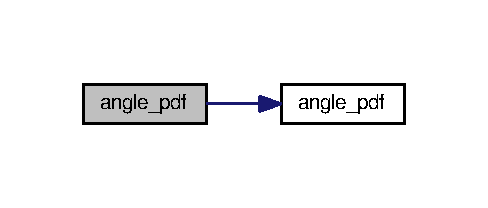
\includegraphics[width=234pt]{_bhabha__fortran__sem__doxy_8f_aea97ae5ed563aa63a80df4f38d19e289_cgraph}
\end{center}
\end{figure}


\index{Bhabha\+\_\+fortran\+\_\+sem\+\_\+doxy.\+f@{Bhabha\+\_\+fortran\+\_\+sem\+\_\+doxy.\+f}!anglit\+\_\+cdf@{anglit\+\_\+cdf}}
\index{anglit\+\_\+cdf@{anglit\+\_\+cdf}!Bhabha\+\_\+fortran\+\_\+sem\+\_\+doxy.\+f@{Bhabha\+\_\+fortran\+\_\+sem\+\_\+doxy.\+f}}
\subsubsection[{\texorpdfstring{anglit\+\_\+cdf(x, cdf)}{anglit_cdf(x, cdf)}}]{\setlength{\rightskip}{0pt plus 5cm}subroutine anglit\+\_\+cdf (
\begin{DoxyParamCaption}
\item[{double precision}]{x, }
\item[{double precision, value}]{cdf}
\end{DoxyParamCaption}
)}\hypertarget{_bhabha__fortran__sem__doxy_8f_ae6f220f29d92fd5e4ac84c22029dcbc5}{}\label{_bhabha__fortran__sem__doxy_8f_ae6f220f29d92fd5e4ac84c22029dcbc5}


Definition at line 396 of file Bhabha\+\_\+fortran\+\_\+sem\+\_\+doxy.\+f.



Here is the call graph for this function\+:\nopagebreak
\begin{figure}[H]
\begin{center}
\leavevmode
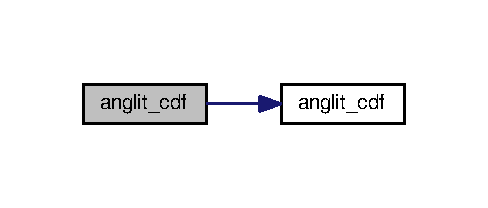
\includegraphics[width=234pt]{_bhabha__fortran__sem__doxy_8f_ae6f220f29d92fd5e4ac84c22029dcbc5_cgraph}
\end{center}
\end{figure}


\index{Bhabha\+\_\+fortran\+\_\+sem\+\_\+doxy.\+f@{Bhabha\+\_\+fortran\+\_\+sem\+\_\+doxy.\+f}!anglit\+\_\+cdf\+\_\+inv@{anglit\+\_\+cdf\+\_\+inv}}
\index{anglit\+\_\+cdf\+\_\+inv@{anglit\+\_\+cdf\+\_\+inv}!Bhabha\+\_\+fortran\+\_\+sem\+\_\+doxy.\+f@{Bhabha\+\_\+fortran\+\_\+sem\+\_\+doxy.\+f}}
\subsubsection[{\texorpdfstring{anglit\+\_\+cdf\+\_\+inv(cdf, x)}{anglit_cdf_inv(cdf, x)}}]{\setlength{\rightskip}{0pt plus 5cm}subroutine anglit\+\_\+cdf\+\_\+inv (
\begin{DoxyParamCaption}
\item[{double precision, value}]{cdf, }
\item[{double precision}]{x}
\end{DoxyParamCaption}
)}\hypertarget{_bhabha__fortran__sem__doxy_8f_aac69fb6d192dd21c8a01a0b768047f59}{}\label{_bhabha__fortran__sem__doxy_8f_aac69fb6d192dd21c8a01a0b768047f59}


Definition at line 437 of file Bhabha\+\_\+fortran\+\_\+sem\+\_\+doxy.\+f.



Here is the call graph for this function\+:\nopagebreak
\begin{figure}[H]
\begin{center}
\leavevmode
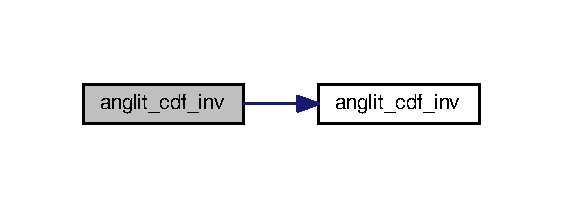
\includegraphics[width=270pt]{_bhabha__fortran__sem__doxy_8f_aac69fb6d192dd21c8a01a0b768047f59_cgraph}
\end{center}
\end{figure}


\index{Bhabha\+\_\+fortran\+\_\+sem\+\_\+doxy.\+f@{Bhabha\+\_\+fortran\+\_\+sem\+\_\+doxy.\+f}!anglit\+\_\+mean@{anglit\+\_\+mean}}
\index{anglit\+\_\+mean@{anglit\+\_\+mean}!Bhabha\+\_\+fortran\+\_\+sem\+\_\+doxy.\+f@{Bhabha\+\_\+fortran\+\_\+sem\+\_\+doxy.\+f}}
\subsubsection[{\texorpdfstring{anglit\+\_\+mean(mean)}{anglit_mean(mean)}}]{\setlength{\rightskip}{0pt plus 5cm}subroutine anglit\+\_\+mean (
\begin{DoxyParamCaption}
\item[{double precision}]{mean}
\end{DoxyParamCaption}
)}\hypertarget{_bhabha__fortran__sem__doxy_8f_aedd5857199140786c9bc4b031062c55e}{}\label{_bhabha__fortran__sem__doxy_8f_aedd5857199140786c9bc4b031062c55e}


Definition at line 480 of file Bhabha\+\_\+fortran\+\_\+sem\+\_\+doxy.\+f.



Here is the call graph for this function\+:\nopagebreak
\begin{figure}[H]
\begin{center}
\leavevmode
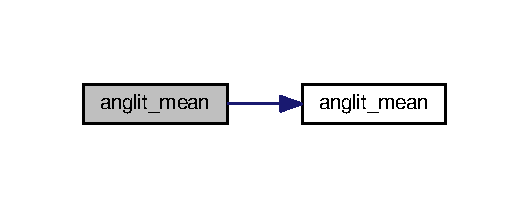
\includegraphics[width=254pt]{_bhabha__fortran__sem__doxy_8f_aedd5857199140786c9bc4b031062c55e_cgraph}
\end{center}
\end{figure}


\index{Bhabha\+\_\+fortran\+\_\+sem\+\_\+doxy.\+f@{Bhabha\+\_\+fortran\+\_\+sem\+\_\+doxy.\+f}!anglit\+\_\+pdf@{anglit\+\_\+pdf}}
\index{anglit\+\_\+pdf@{anglit\+\_\+pdf}!Bhabha\+\_\+fortran\+\_\+sem\+\_\+doxy.\+f@{Bhabha\+\_\+fortran\+\_\+sem\+\_\+doxy.\+f}}
\subsubsection[{\texorpdfstring{anglit\+\_\+pdf(x, pdf)}{anglit_pdf(x, pdf)}}]{\setlength{\rightskip}{0pt plus 5cm}subroutine anglit\+\_\+pdf (
\begin{DoxyParamCaption}
\item[{double precision}]{x, }
\item[{double precision, value}]{pdf}
\end{DoxyParamCaption}
)}\hypertarget{_bhabha__fortran__sem__doxy_8f_a6ac310db648e48aed924a16a04c1ba4e}{}\label{_bhabha__fortran__sem__doxy_8f_a6ac310db648e48aed924a16a04c1ba4e}


Definition at line 510 of file Bhabha\+\_\+fortran\+\_\+sem\+\_\+doxy.\+f.



Here is the call graph for this function\+:\nopagebreak
\begin{figure}[H]
\begin{center}
\leavevmode
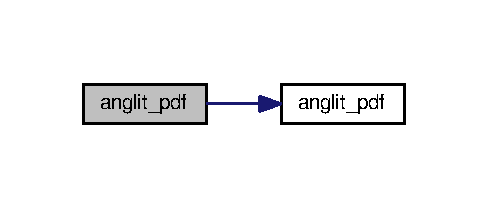
\includegraphics[width=234pt]{_bhabha__fortran__sem__doxy_8f_a6ac310db648e48aed924a16a04c1ba4e_cgraph}
\end{center}
\end{figure}


\index{Bhabha\+\_\+fortran\+\_\+sem\+\_\+doxy.\+f@{Bhabha\+\_\+fortran\+\_\+sem\+\_\+doxy.\+f}!anglit\+\_\+sample@{anglit\+\_\+sample}}
\index{anglit\+\_\+sample@{anglit\+\_\+sample}!Bhabha\+\_\+fortran\+\_\+sem\+\_\+doxy.\+f@{Bhabha\+\_\+fortran\+\_\+sem\+\_\+doxy.\+f}}
\subsubsection[{\texorpdfstring{anglit\+\_\+sample(seed, x)}{anglit_sample(seed, x)}}]{\setlength{\rightskip}{0pt plus 5cm}subroutine anglit\+\_\+sample (
\begin{DoxyParamCaption}
\item[{integer}]{seed, }
\item[{double precision}]{x}
\end{DoxyParamCaption}
)}\hypertarget{_bhabha__fortran__sem__doxy_8f_ad8650a8f15bfee60252281a20c85516e}{}\label{_bhabha__fortran__sem__doxy_8f_ad8650a8f15bfee60252281a20c85516e}


Definition at line 553 of file Bhabha\+\_\+fortran\+\_\+sem\+\_\+doxy.\+f.



Here is the call graph for this function\+:\nopagebreak
\begin{figure}[H]
\begin{center}
\leavevmode
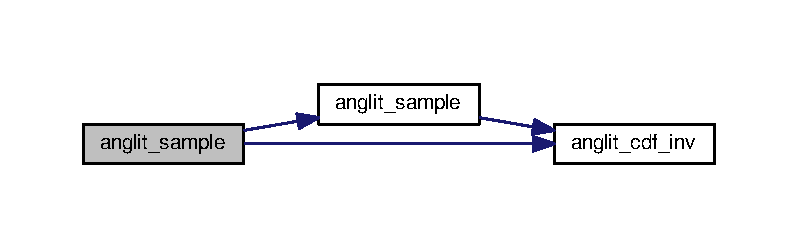
\includegraphics[width=350pt]{_bhabha__fortran__sem__doxy_8f_ad8650a8f15bfee60252281a20c85516e_cgraph}
\end{center}
\end{figure}


\index{Bhabha\+\_\+fortran\+\_\+sem\+\_\+doxy.\+f@{Bhabha\+\_\+fortran\+\_\+sem\+\_\+doxy.\+f}!anglit\+\_\+variance@{anglit\+\_\+variance}}
\index{anglit\+\_\+variance@{anglit\+\_\+variance}!Bhabha\+\_\+fortran\+\_\+sem\+\_\+doxy.\+f@{Bhabha\+\_\+fortran\+\_\+sem\+\_\+doxy.\+f}}
\subsubsection[{\texorpdfstring{anglit\+\_\+variance(variance)}{anglit_variance(variance)}}]{\setlength{\rightskip}{0pt plus 5cm}subroutine anglit\+\_\+variance (
\begin{DoxyParamCaption}
\item[{double precision}]{variance}
\end{DoxyParamCaption}
)}\hypertarget{_bhabha__fortran__sem__doxy_8f_a4e147e31b56df3c9c2751b91de61ba28}{}\label{_bhabha__fortran__sem__doxy_8f_a4e147e31b56df3c9c2751b91de61ba28}


Definition at line 591 of file Bhabha\+\_\+fortran\+\_\+sem\+\_\+doxy.\+f.



Here is the call graph for this function\+:\nopagebreak
\begin{figure}[H]
\begin{center}
\leavevmode
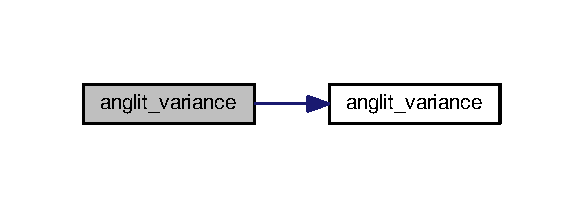
\includegraphics[width=280pt]{_bhabha__fortran__sem__doxy_8f_a4e147e31b56df3c9c2751b91de61ba28_cgraph}
\end{center}
\end{figure}


\index{Bhabha\+\_\+fortran\+\_\+sem\+\_\+doxy.\+f@{Bhabha\+\_\+fortran\+\_\+sem\+\_\+doxy.\+f}!arcsin\+\_\+cdf@{arcsin\+\_\+cdf}}
\index{arcsin\+\_\+cdf@{arcsin\+\_\+cdf}!Bhabha\+\_\+fortran\+\_\+sem\+\_\+doxy.\+f@{Bhabha\+\_\+fortran\+\_\+sem\+\_\+doxy.\+f}}
\subsubsection[{\texorpdfstring{arcsin\+\_\+cdf(x, a, cdf)}{arcsin_cdf(x, a, cdf)}}]{\setlength{\rightskip}{0pt plus 5cm}subroutine arcsin\+\_\+cdf (
\begin{DoxyParamCaption}
\item[{double precision}]{x, }
\item[{double precision}]{a, }
\item[{double precision, parameter, value}]{cdf}
\end{DoxyParamCaption}
)}\hypertarget{_bhabha__fortran__sem__doxy_8f_ad1ea95ee407eec1875a81feb0d44d6e1}{}\label{_bhabha__fortran__sem__doxy_8f_ad1ea95ee407eec1875a81feb0d44d6e1}


Definition at line 632 of file Bhabha\+\_\+fortran\+\_\+sem\+\_\+doxy.\+f.



Here is the call graph for this function\+:\nopagebreak
\begin{figure}[H]
\begin{center}
\leavevmode
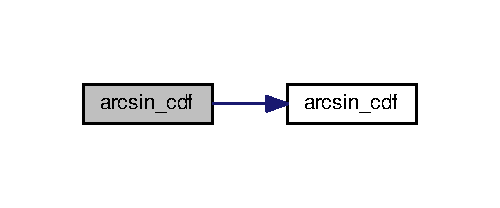
\includegraphics[width=240pt]{_bhabha__fortran__sem__doxy_8f_ad1ea95ee407eec1875a81feb0d44d6e1_cgraph}
\end{center}
\end{figure}


\index{Bhabha\+\_\+fortran\+\_\+sem\+\_\+doxy.\+f@{Bhabha\+\_\+fortran\+\_\+sem\+\_\+doxy.\+f}!arcsin\+\_\+cdf\+\_\+inv@{arcsin\+\_\+cdf\+\_\+inv}}
\index{arcsin\+\_\+cdf\+\_\+inv@{arcsin\+\_\+cdf\+\_\+inv}!Bhabha\+\_\+fortran\+\_\+sem\+\_\+doxy.\+f@{Bhabha\+\_\+fortran\+\_\+sem\+\_\+doxy.\+f}}
\subsubsection[{\texorpdfstring{arcsin\+\_\+cdf\+\_\+inv(cdf, a, x)}{arcsin_cdf_inv(cdf, a, x)}}]{\setlength{\rightskip}{0pt plus 5cm}subroutine arcsin\+\_\+cdf\+\_\+inv (
\begin{DoxyParamCaption}
\item[{double precision, parameter, value}]{cdf, }
\item[{double precision}]{a, }
\item[{double precision}]{x}
\end{DoxyParamCaption}
)}\hypertarget{_bhabha__fortran__sem__doxy_8f_aeba9ed4e4b270a2c19780190aaaed016}{}\label{_bhabha__fortran__sem__doxy_8f_aeba9ed4e4b270a2c19780190aaaed016}


Definition at line 677 of file Bhabha\+\_\+fortran\+\_\+sem\+\_\+doxy.\+f.



Here is the call graph for this function\+:\nopagebreak
\begin{figure}[H]
\begin{center}
\leavevmode
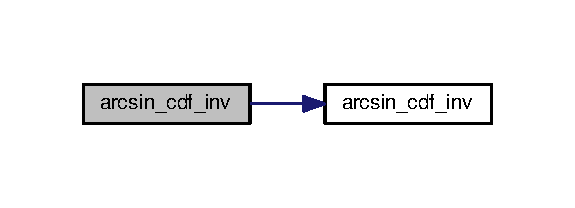
\includegraphics[width=276pt]{_bhabha__fortran__sem__doxy_8f_aeba9ed4e4b270a2c19780190aaaed016_cgraph}
\end{center}
\end{figure}


\index{Bhabha\+\_\+fortran\+\_\+sem\+\_\+doxy.\+f@{Bhabha\+\_\+fortran\+\_\+sem\+\_\+doxy.\+f}!arcsin\+\_\+check@{arcsin\+\_\+check}}
\index{arcsin\+\_\+check@{arcsin\+\_\+check}!Bhabha\+\_\+fortran\+\_\+sem\+\_\+doxy.\+f@{Bhabha\+\_\+fortran\+\_\+sem\+\_\+doxy.\+f}}
\subsubsection[{\texorpdfstring{arcsin\+\_\+check(a)}{arcsin_check(a)}}]{\setlength{\rightskip}{0pt plus 5cm}logical function arcsin\+\_\+check (
\begin{DoxyParamCaption}
\item[{double precision}]{a}
\end{DoxyParamCaption}
)}\hypertarget{_bhabha__fortran__sem__doxy_8f_a6106c25a912dbdfd3a3016548132640e}{}\label{_bhabha__fortran__sem__doxy_8f_a6106c25a912dbdfd3a3016548132640e}


Definition at line 724 of file Bhabha\+\_\+fortran\+\_\+sem\+\_\+doxy.\+f.



Here is the call graph for this function\+:\nopagebreak
\begin{figure}[H]
\begin{center}
\leavevmode
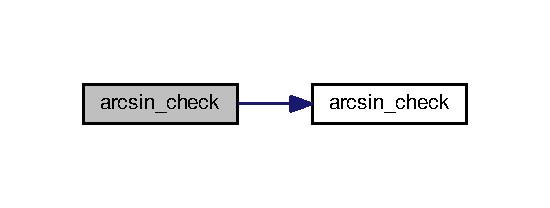
\includegraphics[width=264pt]{_bhabha__fortran__sem__doxy_8f_a6106c25a912dbdfd3a3016548132640e_cgraph}
\end{center}
\end{figure}


\index{Bhabha\+\_\+fortran\+\_\+sem\+\_\+doxy.\+f@{Bhabha\+\_\+fortran\+\_\+sem\+\_\+doxy.\+f}!arcsin\+\_\+mean@{arcsin\+\_\+mean}}
\index{arcsin\+\_\+mean@{arcsin\+\_\+mean}!Bhabha\+\_\+fortran\+\_\+sem\+\_\+doxy.\+f@{Bhabha\+\_\+fortran\+\_\+sem\+\_\+doxy.\+f}}
\subsubsection[{\texorpdfstring{arcsin\+\_\+mean(a, mean)}{arcsin_mean(a, mean)}}]{\setlength{\rightskip}{0pt plus 5cm}subroutine arcsin\+\_\+mean (
\begin{DoxyParamCaption}
\item[{double precision}]{a, }
\item[{double precision}]{mean}
\end{DoxyParamCaption}
)}\hypertarget{_bhabha__fortran__sem__doxy_8f_a0f3f6a9d53c5ee489f35b5aedd71c3e9}{}\label{_bhabha__fortran__sem__doxy_8f_a0f3f6a9d53c5ee489f35b5aedd71c3e9}


Definition at line 766 of file Bhabha\+\_\+fortran\+\_\+sem\+\_\+doxy.\+f.



Here is the call graph for this function\+:\nopagebreak
\begin{figure}[H]
\begin{center}
\leavevmode
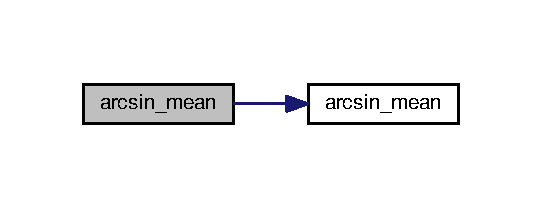
\includegraphics[width=260pt]{_bhabha__fortran__sem__doxy_8f_a0f3f6a9d53c5ee489f35b5aedd71c3e9_cgraph}
\end{center}
\end{figure}


\index{Bhabha\+\_\+fortran\+\_\+sem\+\_\+doxy.\+f@{Bhabha\+\_\+fortran\+\_\+sem\+\_\+doxy.\+f}!arcsin\+\_\+pdf@{arcsin\+\_\+pdf}}
\index{arcsin\+\_\+pdf@{arcsin\+\_\+pdf}!Bhabha\+\_\+fortran\+\_\+sem\+\_\+doxy.\+f@{Bhabha\+\_\+fortran\+\_\+sem\+\_\+doxy.\+f}}
\subsubsection[{\texorpdfstring{arcsin\+\_\+pdf(x, a, pdf)}{arcsin_pdf(x, a, pdf)}}]{\setlength{\rightskip}{0pt plus 5cm}subroutine arcsin\+\_\+pdf (
\begin{DoxyParamCaption}
\item[{double precision}]{x, }
\item[{double precision}]{a, }
\item[{double precision, value}]{pdf}
\end{DoxyParamCaption}
)}\hypertarget{_bhabha__fortran__sem__doxy_8f_a370461195a0a6dbc81d1694f1c900521}{}\label{_bhabha__fortran__sem__doxy_8f_a370461195a0a6dbc81d1694f1c900521}


Definition at line 800 of file Bhabha\+\_\+fortran\+\_\+sem\+\_\+doxy.\+f.



Here is the call graph for this function\+:\nopagebreak
\begin{figure}[H]
\begin{center}
\leavevmode
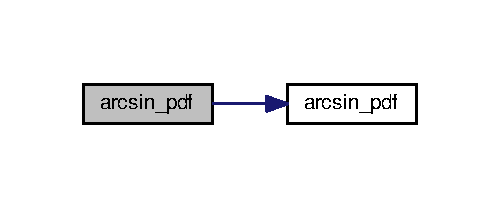
\includegraphics[width=240pt]{_bhabha__fortran__sem__doxy_8f_a370461195a0a6dbc81d1694f1c900521_cgraph}
\end{center}
\end{figure}


\index{Bhabha\+\_\+fortran\+\_\+sem\+\_\+doxy.\+f@{Bhabha\+\_\+fortran\+\_\+sem\+\_\+doxy.\+f}!arcsin\+\_\+sample@{arcsin\+\_\+sample}}
\index{arcsin\+\_\+sample@{arcsin\+\_\+sample}!Bhabha\+\_\+fortran\+\_\+sem\+\_\+doxy.\+f@{Bhabha\+\_\+fortran\+\_\+sem\+\_\+doxy.\+f}}
\subsubsection[{\texorpdfstring{arcsin\+\_\+sample(a, seed, x)}{arcsin_sample(a, seed, x)}}]{\setlength{\rightskip}{0pt plus 5cm}subroutine arcsin\+\_\+sample (
\begin{DoxyParamCaption}
\item[{double precision}]{a, }
\item[{integer}]{seed, }
\item[{double precision}]{x}
\end{DoxyParamCaption}
)}\hypertarget{_bhabha__fortran__sem__doxy_8f_af45217dbb90ff9bd690d7d87061616a9}{}\label{_bhabha__fortran__sem__doxy_8f_af45217dbb90ff9bd690d7d87061616a9}


Definition at line 884 of file Bhabha\+\_\+fortran\+\_\+sem\+\_\+doxy.\+f.



Here is the call graph for this function\+:\nopagebreak
\begin{figure}[H]
\begin{center}
\leavevmode
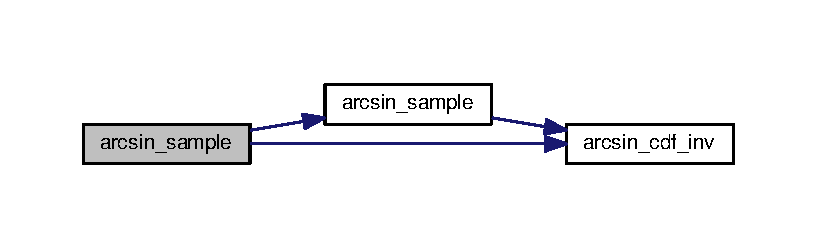
\includegraphics[width=350pt]{_bhabha__fortran__sem__doxy_8f_af45217dbb90ff9bd690d7d87061616a9_cgraph}
\end{center}
\end{figure}


\index{Bhabha\+\_\+fortran\+\_\+sem\+\_\+doxy.\+f@{Bhabha\+\_\+fortran\+\_\+sem\+\_\+doxy.\+f}!arcsin\+\_\+variance@{arcsin\+\_\+variance}}
\index{arcsin\+\_\+variance@{arcsin\+\_\+variance}!Bhabha\+\_\+fortran\+\_\+sem\+\_\+doxy.\+f@{Bhabha\+\_\+fortran\+\_\+sem\+\_\+doxy.\+f}}
\subsubsection[{\texorpdfstring{arcsin\+\_\+variance(a, variance)}{arcsin_variance(a, variance)}}]{\setlength{\rightskip}{0pt plus 5cm}subroutine arcsin\+\_\+variance (
\begin{DoxyParamCaption}
\item[{double precision}]{a, }
\item[{double precision}]{variance}
\end{DoxyParamCaption}
)}\hypertarget{_bhabha__fortran__sem__doxy_8f_aec7db221e74872bf1e854e0bd9bab771}{}\label{_bhabha__fortran__sem__doxy_8f_aec7db221e74872bf1e854e0bd9bab771}


Definition at line 926 of file Bhabha\+\_\+fortran\+\_\+sem\+\_\+doxy.\+f.



Here is the call graph for this function\+:\nopagebreak
\begin{figure}[H]
\begin{center}
\leavevmode
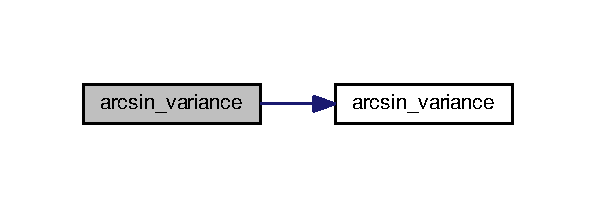
\includegraphics[width=286pt]{_bhabha__fortran__sem__doxy_8f_aec7db221e74872bf1e854e0bd9bab771_cgraph}
\end{center}
\end{figure}


\index{Bhabha\+\_\+fortran\+\_\+sem\+\_\+doxy.\+f@{Bhabha\+\_\+fortran\+\_\+sem\+\_\+doxy.\+f}!benford\+\_\+pdf@{benford\+\_\+pdf}}
\index{benford\+\_\+pdf@{benford\+\_\+pdf}!Bhabha\+\_\+fortran\+\_\+sem\+\_\+doxy.\+f@{Bhabha\+\_\+fortran\+\_\+sem\+\_\+doxy.\+f}}
\subsubsection[{\texorpdfstring{benford\+\_\+pdf(x, pdf)}{benford_pdf(x, pdf)}}]{\setlength{\rightskip}{0pt plus 5cm}subroutine benford\+\_\+pdf (
\begin{DoxyParamCaption}
\item[{double precision}]{x, }
\item[{}]{pdf}
\end{DoxyParamCaption}
)}\hypertarget{_bhabha__fortran__sem__doxy_8f_a9fef702e6bf364a5f85533ca613a7d94}{}\label{_bhabha__fortran__sem__doxy_8f_a9fef702e6bf364a5f85533ca613a7d94}


Definition at line 960 of file Bhabha\+\_\+fortran\+\_\+sem\+\_\+doxy.\+f.



Here is the call graph for this function\+:\nopagebreak
\begin{figure}[H]
\begin{center}
\leavevmode
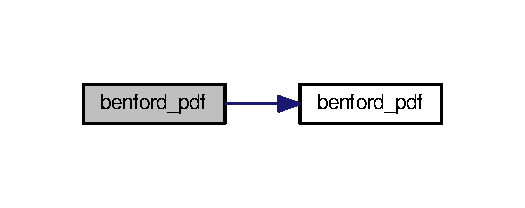
\includegraphics[width=252pt]{_bhabha__fortran__sem__doxy_8f_a9fef702e6bf364a5f85533ca613a7d94_cgraph}
\end{center}
\end{figure}


\index{Bhabha\+\_\+fortran\+\_\+sem\+\_\+doxy.\+f@{Bhabha\+\_\+fortran\+\_\+sem\+\_\+doxy.\+f}!bernoulli\+\_\+cdf@{bernoulli\+\_\+cdf}}
\index{bernoulli\+\_\+cdf@{bernoulli\+\_\+cdf}!Bhabha\+\_\+fortran\+\_\+sem\+\_\+doxy.\+f@{Bhabha\+\_\+fortran\+\_\+sem\+\_\+doxy.\+f}}
\subsubsection[{\texorpdfstring{bernoulli\+\_\+cdf(x, a, cdf)}{bernoulli_cdf(x, a, cdf)}}]{\setlength{\rightskip}{0pt plus 5cm}subroutine bernoulli\+\_\+cdf (
\begin{DoxyParamCaption}
\item[{integer}]{x, }
\item[{double precision}]{a, }
\item[{double precision, value}]{cdf}
\end{DoxyParamCaption}
)}\hypertarget{_bhabha__fortran__sem__doxy_8f_ab0c099a6932ebc7e4d4378e2bcebfb6a}{}\label{_bhabha__fortran__sem__doxy_8f_ab0c099a6932ebc7e4d4378e2bcebfb6a}


Definition at line 1389 of file Bhabha\+\_\+fortran\+\_\+sem\+\_\+doxy.\+f.



Here is the call graph for this function\+:\nopagebreak
\begin{figure}[H]
\begin{center}
\leavevmode
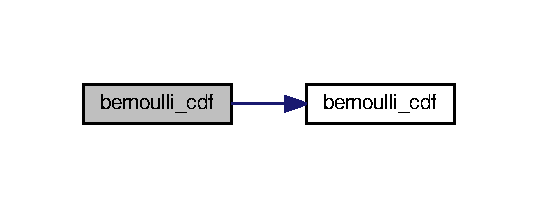
\includegraphics[width=258pt]{_bhabha__fortran__sem__doxy_8f_ab0c099a6932ebc7e4d4378e2bcebfb6a_cgraph}
\end{center}
\end{figure}


\index{Bhabha\+\_\+fortran\+\_\+sem\+\_\+doxy.\+f@{Bhabha\+\_\+fortran\+\_\+sem\+\_\+doxy.\+f}!bernoulli\+\_\+cdf\+\_\+inv@{bernoulli\+\_\+cdf\+\_\+inv}}
\index{bernoulli\+\_\+cdf\+\_\+inv@{bernoulli\+\_\+cdf\+\_\+inv}!Bhabha\+\_\+fortran\+\_\+sem\+\_\+doxy.\+f@{Bhabha\+\_\+fortran\+\_\+sem\+\_\+doxy.\+f}}
\subsubsection[{\texorpdfstring{bernoulli\+\_\+cdf\+\_\+inv(cdf, a, x)}{bernoulli_cdf_inv(cdf, a, x)}}]{\setlength{\rightskip}{0pt plus 5cm}subroutine bernoulli\+\_\+cdf\+\_\+inv (
\begin{DoxyParamCaption}
\item[{double precision, value}]{cdf, }
\item[{double precision}]{a, }
\item[{integer}]{x}
\end{DoxyParamCaption}
)}\hypertarget{_bhabha__fortran__sem__doxy_8f_aba46047e0d6d0160e9e7f72f468fada8}{}\label{_bhabha__fortran__sem__doxy_8f_aba46047e0d6d0160e9e7f72f468fada8}


Definition at line 1433 of file Bhabha\+\_\+fortran\+\_\+sem\+\_\+doxy.\+f.



Here is the call graph for this function\+:\nopagebreak
\begin{figure}[H]
\begin{center}
\leavevmode
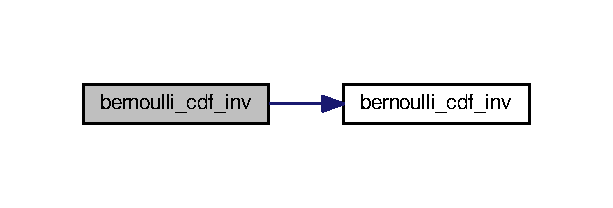
\includegraphics[width=294pt]{_bhabha__fortran__sem__doxy_8f_aba46047e0d6d0160e9e7f72f468fada8_cgraph}
\end{center}
\end{figure}


\index{Bhabha\+\_\+fortran\+\_\+sem\+\_\+doxy.\+f@{Bhabha\+\_\+fortran\+\_\+sem\+\_\+doxy.\+f}!bernoulli\+\_\+check@{bernoulli\+\_\+check}}
\index{bernoulli\+\_\+check@{bernoulli\+\_\+check}!Bhabha\+\_\+fortran\+\_\+sem\+\_\+doxy.\+f@{Bhabha\+\_\+fortran\+\_\+sem\+\_\+doxy.\+f}}
\subsubsection[{\texorpdfstring{bernoulli\+\_\+check(a)}{bernoulli_check(a)}}]{\setlength{\rightskip}{0pt plus 5cm}logical function bernoulli\+\_\+check (
\begin{DoxyParamCaption}
\item[{double precision}]{a}
\end{DoxyParamCaption}
)}\hypertarget{_bhabha__fortran__sem__doxy_8f_ab60b2073960d9ea664fad920aaccfb29}{}\label{_bhabha__fortran__sem__doxy_8f_ab60b2073960d9ea664fad920aaccfb29}


Definition at line 1482 of file Bhabha\+\_\+fortran\+\_\+sem\+\_\+doxy.\+f.



Here is the call graph for this function\+:\nopagebreak
\begin{figure}[H]
\begin{center}
\leavevmode
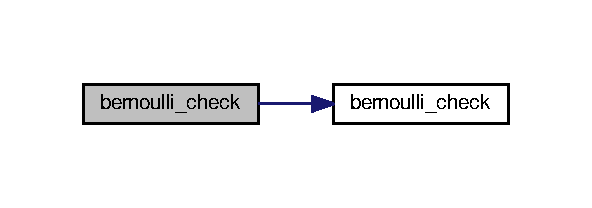
\includegraphics[width=284pt]{_bhabha__fortran__sem__doxy_8f_ab60b2073960d9ea664fad920aaccfb29_cgraph}
\end{center}
\end{figure}


\index{Bhabha\+\_\+fortran\+\_\+sem\+\_\+doxy.\+f@{Bhabha\+\_\+fortran\+\_\+sem\+\_\+doxy.\+f}!bernoulli\+\_\+mean@{bernoulli\+\_\+mean}}
\index{bernoulli\+\_\+mean@{bernoulli\+\_\+mean}!Bhabha\+\_\+fortran\+\_\+sem\+\_\+doxy.\+f@{Bhabha\+\_\+fortran\+\_\+sem\+\_\+doxy.\+f}}
\subsubsection[{\texorpdfstring{bernoulli\+\_\+mean(a, mean)}{bernoulli_mean(a, mean)}}]{\setlength{\rightskip}{0pt plus 5cm}subroutine bernoulli\+\_\+mean (
\begin{DoxyParamCaption}
\item[{double precision}]{a, }
\item[{double precision}]{mean}
\end{DoxyParamCaption}
)}\hypertarget{_bhabha__fortran__sem__doxy_8f_a0b4283a0687fb97d4b5e37594d3d960e}{}\label{_bhabha__fortran__sem__doxy_8f_a0b4283a0687fb97d4b5e37594d3d960e}


Definition at line 1524 of file Bhabha\+\_\+fortran\+\_\+sem\+\_\+doxy.\+f.



Here is the call graph for this function\+:\nopagebreak
\begin{figure}[H]
\begin{center}
\leavevmode
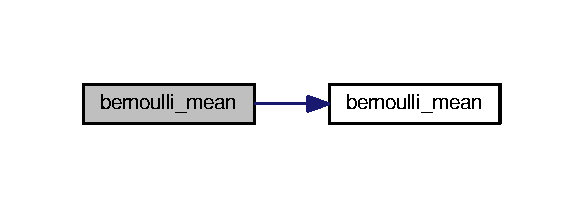
\includegraphics[width=280pt]{_bhabha__fortran__sem__doxy_8f_a0b4283a0687fb97d4b5e37594d3d960e_cgraph}
\end{center}
\end{figure}


\index{Bhabha\+\_\+fortran\+\_\+sem\+\_\+doxy.\+f@{Bhabha\+\_\+fortran\+\_\+sem\+\_\+doxy.\+f}!bernoulli\+\_\+pdf@{bernoulli\+\_\+pdf}}
\index{bernoulli\+\_\+pdf@{bernoulli\+\_\+pdf}!Bhabha\+\_\+fortran\+\_\+sem\+\_\+doxy.\+f@{Bhabha\+\_\+fortran\+\_\+sem\+\_\+doxy.\+f}}
\subsubsection[{\texorpdfstring{bernoulli\+\_\+pdf(x, a, pdf)}{bernoulli_pdf(x, a, pdf)}}]{\setlength{\rightskip}{0pt plus 5cm}subroutine bernoulli\+\_\+pdf (
\begin{DoxyParamCaption}
\item[{integer}]{x, }
\item[{double precision}]{a, }
\item[{double precision, value}]{pdf}
\end{DoxyParamCaption}
)}\hypertarget{_bhabha__fortran__sem__doxy_8f_a89fa5f5a4cbaa3ec07e13d430cdbb0b8}{}\label{_bhabha__fortran__sem__doxy_8f_a89fa5f5a4cbaa3ec07e13d430cdbb0b8}


Definition at line 1558 of file Bhabha\+\_\+fortran\+\_\+sem\+\_\+doxy.\+f.



Here is the call graph for this function\+:\nopagebreak
\begin{figure}[H]
\begin{center}
\leavevmode
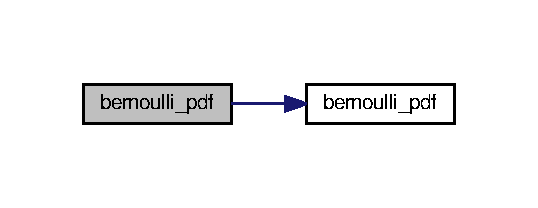
\includegraphics[width=258pt]{_bhabha__fortran__sem__doxy_8f_a89fa5f5a4cbaa3ec07e13d430cdbb0b8_cgraph}
\end{center}
\end{figure}


\index{Bhabha\+\_\+fortran\+\_\+sem\+\_\+doxy.\+f@{Bhabha\+\_\+fortran\+\_\+sem\+\_\+doxy.\+f}!bernoulli\+\_\+sample@{bernoulli\+\_\+sample}}
\index{bernoulli\+\_\+sample@{bernoulli\+\_\+sample}!Bhabha\+\_\+fortran\+\_\+sem\+\_\+doxy.\+f@{Bhabha\+\_\+fortran\+\_\+sem\+\_\+doxy.\+f}}
\subsubsection[{\texorpdfstring{bernoulli\+\_\+sample(a, seed, x)}{bernoulli_sample(a, seed, x)}}]{\setlength{\rightskip}{0pt plus 5cm}subroutine bernoulli\+\_\+sample (
\begin{DoxyParamCaption}
\item[{double precision}]{a, }
\item[{integer}]{seed, }
\item[{integer}]{x}
\end{DoxyParamCaption}
)}\hypertarget{_bhabha__fortran__sem__doxy_8f_ae46a4cd68c1ca43b8cd6149a3af3451c}{}\label{_bhabha__fortran__sem__doxy_8f_ae46a4cd68c1ca43b8cd6149a3af3451c}


Definition at line 1614 of file Bhabha\+\_\+fortran\+\_\+sem\+\_\+doxy.\+f.



Here is the call graph for this function\+:\nopagebreak
\begin{figure}[H]
\begin{center}
\leavevmode
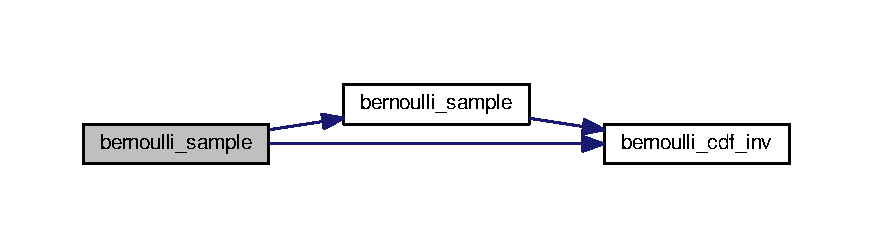
\includegraphics[width=350pt]{_bhabha__fortran__sem__doxy_8f_ae46a4cd68c1ca43b8cd6149a3af3451c_cgraph}
\end{center}
\end{figure}


\index{Bhabha\+\_\+fortran\+\_\+sem\+\_\+doxy.\+f@{Bhabha\+\_\+fortran\+\_\+sem\+\_\+doxy.\+f}!bernoulli\+\_\+variance@{bernoulli\+\_\+variance}}
\index{bernoulli\+\_\+variance@{bernoulli\+\_\+variance}!Bhabha\+\_\+fortran\+\_\+sem\+\_\+doxy.\+f@{Bhabha\+\_\+fortran\+\_\+sem\+\_\+doxy.\+f}}
\subsubsection[{\texorpdfstring{bernoulli\+\_\+variance(a, variance)}{bernoulli_variance(a, variance)}}]{\setlength{\rightskip}{0pt plus 5cm}subroutine bernoulli\+\_\+variance (
\begin{DoxyParamCaption}
\item[{double precision}]{a, }
\item[{double precision}]{variance}
\end{DoxyParamCaption}
)}\hypertarget{_bhabha__fortran__sem__doxy_8f_aac79468ade583fbf0b0faf3fab44bc96}{}\label{_bhabha__fortran__sem__doxy_8f_aac79468ade583fbf0b0faf3fab44bc96}


Definition at line 1656 of file Bhabha\+\_\+fortran\+\_\+sem\+\_\+doxy.\+f.



Here is the call graph for this function\+:\nopagebreak
\begin{figure}[H]
\begin{center}
\leavevmode
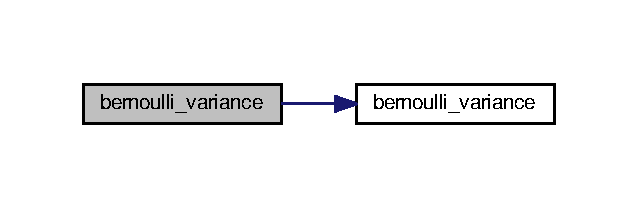
\includegraphics[width=306pt]{_bhabha__fortran__sem__doxy_8f_aac79468ade583fbf0b0faf3fab44bc96_cgraph}
\end{center}
\end{figure}


\index{Bhabha\+\_\+fortran\+\_\+sem\+\_\+doxy.\+f@{Bhabha\+\_\+fortran\+\_\+sem\+\_\+doxy.\+f}!bessel\+\_\+i0@{bessel\+\_\+i0}}
\index{bessel\+\_\+i0@{bessel\+\_\+i0}!Bhabha\+\_\+fortran\+\_\+sem\+\_\+doxy.\+f@{Bhabha\+\_\+fortran\+\_\+sem\+\_\+doxy.\+f}}
\subsubsection[{\texorpdfstring{bessel\+\_\+i0(arg)}{bessel_i0(arg)}}]{\setlength{\rightskip}{0pt plus 5cm}double precision function bessel\+\_\+i0 (
\begin{DoxyParamCaption}
\item[{double precision}]{arg}
\end{DoxyParamCaption}
)}\hypertarget{_bhabha__fortran__sem__doxy_8f_a56f2ab001fb7fd87fd8c17369a866f5a}{}\label{_bhabha__fortran__sem__doxy_8f_a56f2ab001fb7fd87fd8c17369a866f5a}


Definition at line 1690 of file Bhabha\+\_\+fortran\+\_\+sem\+\_\+doxy.\+f.



Here is the call graph for this function\+:\nopagebreak
\begin{figure}[H]
\begin{center}
\leavevmode
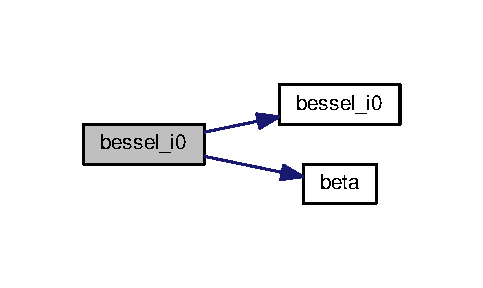
\includegraphics[width=232pt]{_bhabha__fortran__sem__doxy_8f_a56f2ab001fb7fd87fd8c17369a866f5a_cgraph}
\end{center}
\end{figure}


\index{Bhabha\+\_\+fortran\+\_\+sem\+\_\+doxy.\+f@{Bhabha\+\_\+fortran\+\_\+sem\+\_\+doxy.\+f}!bessel\+\_\+i0\+\_\+values@{bessel\+\_\+i0\+\_\+values}}
\index{bessel\+\_\+i0\+\_\+values@{bessel\+\_\+i0\+\_\+values}!Bhabha\+\_\+fortran\+\_\+sem\+\_\+doxy.\+f@{Bhabha\+\_\+fortran\+\_\+sem\+\_\+doxy.\+f}}
\subsubsection[{\texorpdfstring{bessel\+\_\+i0\+\_\+values(n\+\_\+data, x, fx)}{bessel_i0_values(n_data, x, fx)}}]{\setlength{\rightskip}{0pt plus 5cm}subroutine bessel\+\_\+i0\+\_\+values (
\begin{DoxyParamCaption}
\item[{integer, value}]{n\+\_\+data, }
\item[{double precision}]{x, }
\item[{double precision}]{fx}
\end{DoxyParamCaption}
)}\hypertarget{_bhabha__fortran__sem__doxy_8f_a0508ca5dc920b3b002ac4d769e9e7128}{}\label{_bhabha__fortran__sem__doxy_8f_a0508ca5dc920b3b002ac4d769e9e7128}


Definition at line 1875 of file Bhabha\+\_\+fortran\+\_\+sem\+\_\+doxy.\+f.



Here is the call graph for this function\+:\nopagebreak
\begin{figure}[H]
\begin{center}
\leavevmode
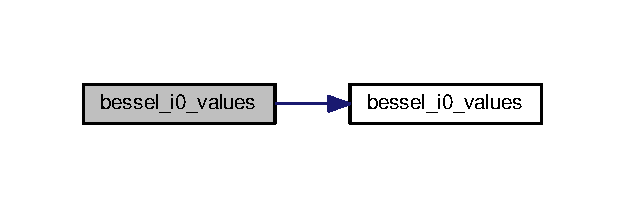
\includegraphics[width=300pt]{_bhabha__fortran__sem__doxy_8f_a0508ca5dc920b3b002ac4d769e9e7128_cgraph}
\end{center}
\end{figure}


\index{Bhabha\+\_\+fortran\+\_\+sem\+\_\+doxy.\+f@{Bhabha\+\_\+fortran\+\_\+sem\+\_\+doxy.\+f}!beta@{beta}}
\index{beta@{beta}!Bhabha\+\_\+fortran\+\_\+sem\+\_\+doxy.\+f@{Bhabha\+\_\+fortran\+\_\+sem\+\_\+doxy.\+f}}
\subsubsection[{\texorpdfstring{beta(a, b)}{beta(a, b)}}]{\setlength{\rightskip}{0pt plus 5cm}double precision function, value beta (
\begin{DoxyParamCaption}
\item[{double precision}]{a, }
\item[{double precision}]{b}
\end{DoxyParamCaption}
)}\hypertarget{_bhabha__fortran__sem__doxy_8f_a4545c4482f31f1e6eddae40f6ed6bbfb}{}\label{_bhabha__fortran__sem__doxy_8f_a4545c4482f31f1e6eddae40f6ed6bbfb}


Definition at line 2320 of file Bhabha\+\_\+fortran\+\_\+sem\+\_\+doxy.\+f.



Here is the call graph for this function\+:\nopagebreak
\begin{figure}[H]
\begin{center}
\leavevmode
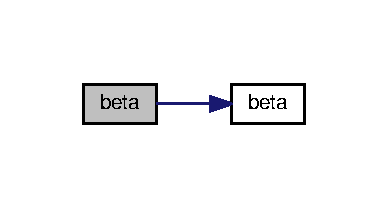
\includegraphics[width=186pt]{_bhabha__fortran__sem__doxy_8f_a4545c4482f31f1e6eddae40f6ed6bbfb_cgraph}
\end{center}
\end{figure}


\index{Bhabha\+\_\+fortran\+\_\+sem\+\_\+doxy.\+f@{Bhabha\+\_\+fortran\+\_\+sem\+\_\+doxy.\+f}!beta\+\_\+binomial\+\_\+cdf@{beta\+\_\+binomial\+\_\+cdf}}
\index{beta\+\_\+binomial\+\_\+cdf@{beta\+\_\+binomial\+\_\+cdf}!Bhabha\+\_\+fortran\+\_\+sem\+\_\+doxy.\+f@{Bhabha\+\_\+fortran\+\_\+sem\+\_\+doxy.\+f}}
\subsubsection[{\texorpdfstring{beta\+\_\+binomial\+\_\+cdf(x, a, b, c, cdf)}{beta_binomial_cdf(x, a, b, c, cdf)}}]{\setlength{\rightskip}{0pt plus 5cm}subroutine beta\+\_\+binomial\+\_\+cdf (
\begin{DoxyParamCaption}
\item[{integer}]{x, }
\item[{double precision}]{a, }
\item[{double precision}]{b, }
\item[{integer}]{c, }
\item[{double precision, value}]{cdf}
\end{DoxyParamCaption}
)}\hypertarget{_bhabha__fortran__sem__doxy_8f_ab79beb1b437d17ea84c53e4d40471f80}{}\label{_bhabha__fortran__sem__doxy_8f_ab79beb1b437d17ea84c53e4d40471f80}


Definition at line 2372 of file Bhabha\+\_\+fortran\+\_\+sem\+\_\+doxy.\+f.



Here is the call graph for this function\+:\nopagebreak
\begin{figure}[H]
\begin{center}
\leavevmode
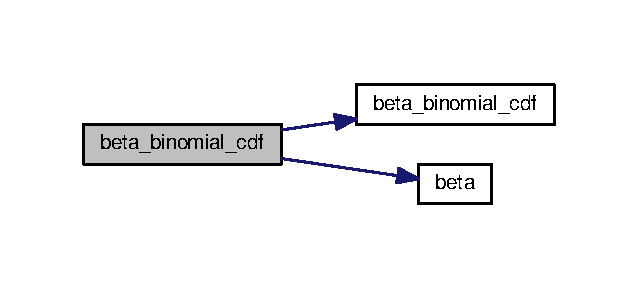
\includegraphics[width=306pt]{_bhabha__fortran__sem__doxy_8f_ab79beb1b437d17ea84c53e4d40471f80_cgraph}
\end{center}
\end{figure}


\index{Bhabha\+\_\+fortran\+\_\+sem\+\_\+doxy.\+f@{Bhabha\+\_\+fortran\+\_\+sem\+\_\+doxy.\+f}!beta\+\_\+binomial\+\_\+cdf\+\_\+inv@{beta\+\_\+binomial\+\_\+cdf\+\_\+inv}}
\index{beta\+\_\+binomial\+\_\+cdf\+\_\+inv@{beta\+\_\+binomial\+\_\+cdf\+\_\+inv}!Bhabha\+\_\+fortran\+\_\+sem\+\_\+doxy.\+f@{Bhabha\+\_\+fortran\+\_\+sem\+\_\+doxy.\+f}}
\subsubsection[{\texorpdfstring{beta\+\_\+binomial\+\_\+cdf\+\_\+inv(cdf, a, b, c, x)}{beta_binomial_cdf_inv(cdf, a, b, c, x)}}]{\setlength{\rightskip}{0pt plus 5cm}subroutine beta\+\_\+binomial\+\_\+cdf\+\_\+inv (
\begin{DoxyParamCaption}
\item[{double precision, value}]{cdf, }
\item[{double precision}]{a, }
\item[{double precision}]{b, }
\item[{integer}]{c, }
\item[{integer}]{x}
\end{DoxyParamCaption}
)}\hypertarget{_bhabha__fortran__sem__doxy_8f_ae6870b2fc15398bbb52dd3b2ed8c92fb}{}\label{_bhabha__fortran__sem__doxy_8f_ae6870b2fc15398bbb52dd3b2ed8c92fb}


Definition at line 2441 of file Bhabha\+\_\+fortran\+\_\+sem\+\_\+doxy.\+f.



Here is the call graph for this function\+:\nopagebreak
\begin{figure}[H]
\begin{center}
\leavevmode
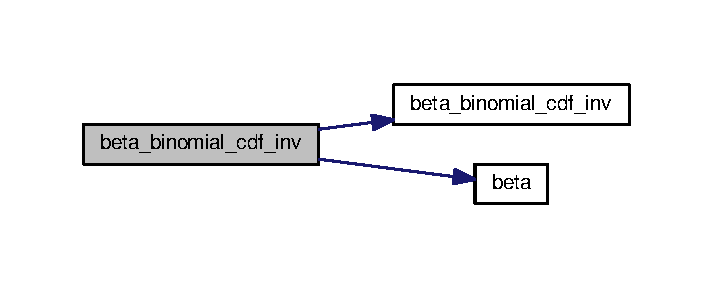
\includegraphics[width=342pt]{_bhabha__fortran__sem__doxy_8f_ae6870b2fc15398bbb52dd3b2ed8c92fb_cgraph}
\end{center}
\end{figure}


\index{Bhabha\+\_\+fortran\+\_\+sem\+\_\+doxy.\+f@{Bhabha\+\_\+fortran\+\_\+sem\+\_\+doxy.\+f}!beta\+\_\+binomial\+\_\+check@{beta\+\_\+binomial\+\_\+check}}
\index{beta\+\_\+binomial\+\_\+check@{beta\+\_\+binomial\+\_\+check}!Bhabha\+\_\+fortran\+\_\+sem\+\_\+doxy.\+f@{Bhabha\+\_\+fortran\+\_\+sem\+\_\+doxy.\+f}}
\subsubsection[{\texorpdfstring{beta\+\_\+binomial\+\_\+check(a, b, c)}{beta_binomial_check(a, b, c)}}]{\setlength{\rightskip}{0pt plus 5cm}logical function beta\+\_\+binomial\+\_\+check (
\begin{DoxyParamCaption}
\item[{double precision}]{a, }
\item[{double precision}]{b, }
\item[{integer}]{c}
\end{DoxyParamCaption}
)}\hypertarget{_bhabha__fortran__sem__doxy_8f_a35d163e54f3880b3b4a4fc1c46ec6690}{}\label{_bhabha__fortran__sem__doxy_8f_a35d163e54f3880b3b4a4fc1c46ec6690}


Definition at line 2518 of file Bhabha\+\_\+fortran\+\_\+sem\+\_\+doxy.\+f.



Here is the call graph for this function\+:\nopagebreak
\begin{figure}[H]
\begin{center}
\leavevmode
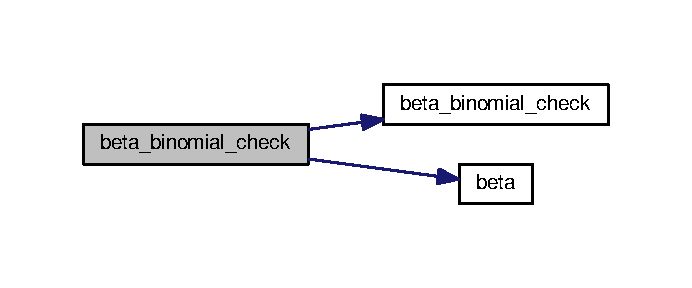
\includegraphics[width=332pt]{_bhabha__fortran__sem__doxy_8f_a35d163e54f3880b3b4a4fc1c46ec6690_cgraph}
\end{center}
\end{figure}


\index{Bhabha\+\_\+fortran\+\_\+sem\+\_\+doxy.\+f@{Bhabha\+\_\+fortran\+\_\+sem\+\_\+doxy.\+f}!beta\+\_\+binomial\+\_\+mean@{beta\+\_\+binomial\+\_\+mean}}
\index{beta\+\_\+binomial\+\_\+mean@{beta\+\_\+binomial\+\_\+mean}!Bhabha\+\_\+fortran\+\_\+sem\+\_\+doxy.\+f@{Bhabha\+\_\+fortran\+\_\+sem\+\_\+doxy.\+f}}
\subsubsection[{\texorpdfstring{beta\+\_\+binomial\+\_\+mean(a, b, c, mean)}{beta_binomial_mean(a, b, c, mean)}}]{\setlength{\rightskip}{0pt plus 5cm}subroutine beta\+\_\+binomial\+\_\+mean (
\begin{DoxyParamCaption}
\item[{double precision}]{a, }
\item[{double precision}]{b, }
\item[{integer}]{c, }
\item[{double precision}]{mean}
\end{DoxyParamCaption}
)}\hypertarget{_bhabha__fortran__sem__doxy_8f_af4c24e7e5f9bebb7bde58f72d2d0bef1}{}\label{_bhabha__fortran__sem__doxy_8f_af4c24e7e5f9bebb7bde58f72d2d0bef1}


Definition at line 2582 of file Bhabha\+\_\+fortran\+\_\+sem\+\_\+doxy.\+f.



Here is the call graph for this function\+:\nopagebreak
\begin{figure}[H]
\begin{center}
\leavevmode
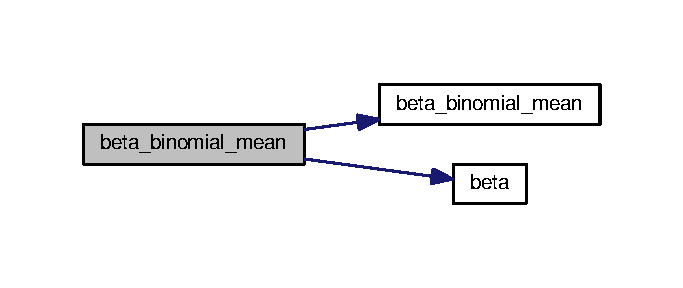
\includegraphics[width=328pt]{_bhabha__fortran__sem__doxy_8f_af4c24e7e5f9bebb7bde58f72d2d0bef1_cgraph}
\end{center}
\end{figure}


\index{Bhabha\+\_\+fortran\+\_\+sem\+\_\+doxy.\+f@{Bhabha\+\_\+fortran\+\_\+sem\+\_\+doxy.\+f}!beta\+\_\+binomial\+\_\+pdf@{beta\+\_\+binomial\+\_\+pdf}}
\index{beta\+\_\+binomial\+\_\+pdf@{beta\+\_\+binomial\+\_\+pdf}!Bhabha\+\_\+fortran\+\_\+sem\+\_\+doxy.\+f@{Bhabha\+\_\+fortran\+\_\+sem\+\_\+doxy.\+f}}
\subsubsection[{\texorpdfstring{beta\+\_\+binomial\+\_\+pdf(x, a, b, c, pdf)}{beta_binomial_pdf(x, a, b, c, pdf)}}]{\setlength{\rightskip}{0pt plus 5cm}subroutine beta\+\_\+binomial\+\_\+pdf (
\begin{DoxyParamCaption}
\item[{integer}]{x, }
\item[{double precision}]{a, }
\item[{double precision}]{b, }
\item[{integer}]{c, }
\item[{double precision, parameter, value}]{pdf}
\end{DoxyParamCaption}
)}\hypertarget{_bhabha__fortran__sem__doxy_8f_a0b1b4e2bbf9c50969318fac23e17215c}{}\label{_bhabha__fortran__sem__doxy_8f_a0b1b4e2bbf9c50969318fac23e17215c}


Definition at line 2622 of file Bhabha\+\_\+fortran\+\_\+sem\+\_\+doxy.\+f.



Here is the call graph for this function\+:\nopagebreak
\begin{figure}[H]
\begin{center}
\leavevmode
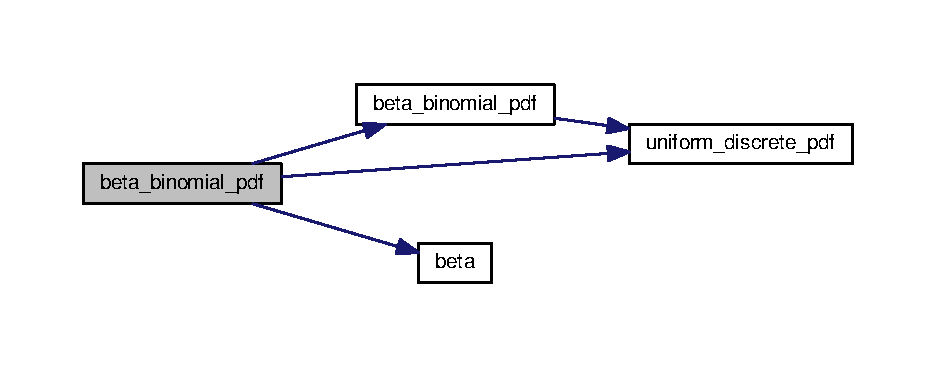
\includegraphics[width=350pt]{_bhabha__fortran__sem__doxy_8f_a0b1b4e2bbf9c50969318fac23e17215c_cgraph}
\end{center}
\end{figure}


\index{Bhabha\+\_\+fortran\+\_\+sem\+\_\+doxy.\+f@{Bhabha\+\_\+fortran\+\_\+sem\+\_\+doxy.\+f}!beta\+\_\+binomial\+\_\+sample@{beta\+\_\+binomial\+\_\+sample}}
\index{beta\+\_\+binomial\+\_\+sample@{beta\+\_\+binomial\+\_\+sample}!Bhabha\+\_\+fortran\+\_\+sem\+\_\+doxy.\+f@{Bhabha\+\_\+fortran\+\_\+sem\+\_\+doxy.\+f}}
\subsubsection[{\texorpdfstring{beta\+\_\+binomial\+\_\+sample(a, b, c, seed, x)}{beta_binomial_sample(a, b, c, seed, x)}}]{\setlength{\rightskip}{0pt plus 5cm}subroutine beta\+\_\+binomial\+\_\+sample (
\begin{DoxyParamCaption}
\item[{double precision}]{a, }
\item[{double precision}]{b, }
\item[{integer}]{c, }
\item[{integer}]{seed, }
\item[{integer}]{x}
\end{DoxyParamCaption}
)}\hypertarget{_bhabha__fortran__sem__doxy_8f_ad097654db5e79584fe38d2a53c8ffad8}{}\label{_bhabha__fortran__sem__doxy_8f_ad097654db5e79584fe38d2a53c8ffad8}


Definition at line 2723 of file Bhabha\+\_\+fortran\+\_\+sem\+\_\+doxy.\+f.



Here is the call graph for this function\+:\nopagebreak
\begin{figure}[H]
\begin{center}
\leavevmode
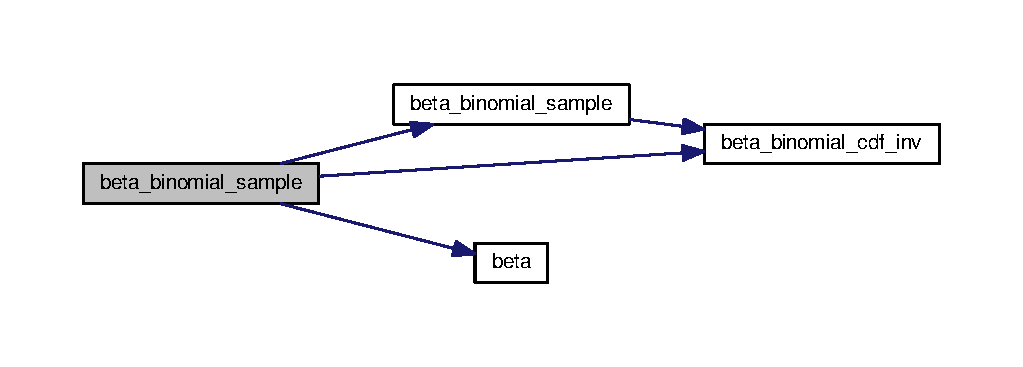
\includegraphics[width=350pt]{_bhabha__fortran__sem__doxy_8f_ad097654db5e79584fe38d2a53c8ffad8_cgraph}
\end{center}
\end{figure}


\index{Bhabha\+\_\+fortran\+\_\+sem\+\_\+doxy.\+f@{Bhabha\+\_\+fortran\+\_\+sem\+\_\+doxy.\+f}!beta\+\_\+binomial\+\_\+variance@{beta\+\_\+binomial\+\_\+variance}}
\index{beta\+\_\+binomial\+\_\+variance@{beta\+\_\+binomial\+\_\+variance}!Bhabha\+\_\+fortran\+\_\+sem\+\_\+doxy.\+f@{Bhabha\+\_\+fortran\+\_\+sem\+\_\+doxy.\+f}}
\subsubsection[{\texorpdfstring{beta\+\_\+binomial\+\_\+variance(a, b, c, variance)}{beta_binomial_variance(a, b, c, variance)}}]{\setlength{\rightskip}{0pt plus 5cm}subroutine beta\+\_\+binomial\+\_\+variance (
\begin{DoxyParamCaption}
\item[{double precision}]{a, }
\item[{double precision}]{b, }
\item[{integer}]{c, }
\item[{double precision}]{variance}
\end{DoxyParamCaption}
)}\hypertarget{_bhabha__fortran__sem__doxy_8f_af18db84101609c96170537b5e09fab18}{}\label{_bhabha__fortran__sem__doxy_8f_af18db84101609c96170537b5e09fab18}


Definition at line 2771 of file Bhabha\+\_\+fortran\+\_\+sem\+\_\+doxy.\+f.



Here is the call graph for this function\+:\nopagebreak
\begin{figure}[H]
\begin{center}
\leavevmode
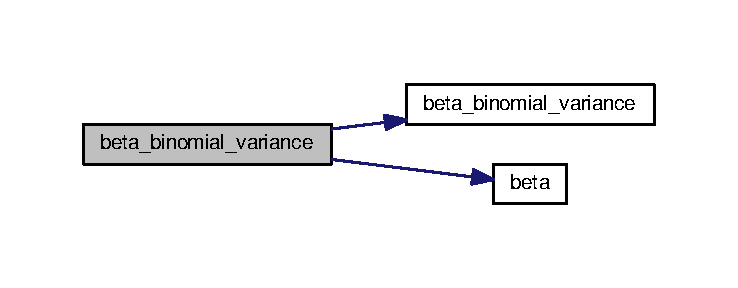
\includegraphics[width=350pt]{_bhabha__fortran__sem__doxy_8f_af18db84101609c96170537b5e09fab18_cgraph}
\end{center}
\end{figure}


\index{Bhabha\+\_\+fortran\+\_\+sem\+\_\+doxy.\+f@{Bhabha\+\_\+fortran\+\_\+sem\+\_\+doxy.\+f}!beta\+\_\+cdf@{beta\+\_\+cdf}}
\index{beta\+\_\+cdf@{beta\+\_\+cdf}!Bhabha\+\_\+fortran\+\_\+sem\+\_\+doxy.\+f@{Bhabha\+\_\+fortran\+\_\+sem\+\_\+doxy.\+f}}
\subsubsection[{\texorpdfstring{beta\+\_\+cdf(x, a, b, cdf)}{beta_cdf(x, a, b, cdf)}}]{\setlength{\rightskip}{0pt plus 5cm}subroutine beta\+\_\+cdf (
\begin{DoxyParamCaption}
\item[{double precision}]{x, }
\item[{double precision}]{a, }
\item[{double precision}]{b, }
\item[{double precision, value}]{cdf}
\end{DoxyParamCaption}
)}\hypertarget{_bhabha__fortran__sem__doxy_8f_a1307bf242705ab2dc0a8db7fc66f4128}{}\label{_bhabha__fortran__sem__doxy_8f_a1307bf242705ab2dc0a8db7fc66f4128}


Definition at line 2813 of file Bhabha\+\_\+fortran\+\_\+sem\+\_\+doxy.\+f.



Here is the call graph for this function\+:\nopagebreak
\begin{figure}[H]
\begin{center}
\leavevmode
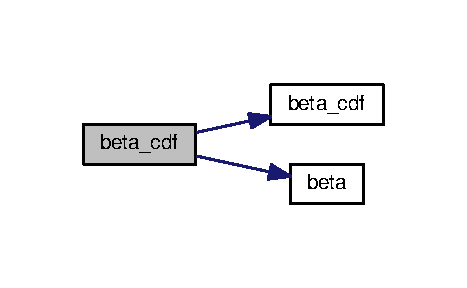
\includegraphics[width=224pt]{_bhabha__fortran__sem__doxy_8f_a1307bf242705ab2dc0a8db7fc66f4128_cgraph}
\end{center}
\end{figure}


\index{Bhabha\+\_\+fortran\+\_\+sem\+\_\+doxy.\+f@{Bhabha\+\_\+fortran\+\_\+sem\+\_\+doxy.\+f}!beta\+\_\+cdf\+\_\+inv@{beta\+\_\+cdf\+\_\+inv}}
\index{beta\+\_\+cdf\+\_\+inv@{beta\+\_\+cdf\+\_\+inv}!Bhabha\+\_\+fortran\+\_\+sem\+\_\+doxy.\+f@{Bhabha\+\_\+fortran\+\_\+sem\+\_\+doxy.\+f}}
\subsubsection[{\texorpdfstring{beta\+\_\+cdf\+\_\+inv(cdf, p, q, x)}{beta_cdf_inv(cdf, p, q, x)}}]{\setlength{\rightskip}{0pt plus 5cm}subroutine beta\+\_\+cdf\+\_\+inv (
\begin{DoxyParamCaption}
\item[{double precision, value}]{cdf, }
\item[{double precision}]{p, }
\item[{double precision}]{q, }
\item[{double precision}]{x}
\end{DoxyParamCaption}
)}\hypertarget{_bhabha__fortran__sem__doxy_8f_ad7b9df743251c691af6f3c722fc44a70}{}\label{_bhabha__fortran__sem__doxy_8f_ad7b9df743251c691af6f3c722fc44a70}


Definition at line 2859 of file Bhabha\+\_\+fortran\+\_\+sem\+\_\+doxy.\+f.



Here is the call graph for this function\+:\nopagebreak
\begin{figure}[H]
\begin{center}
\leavevmode
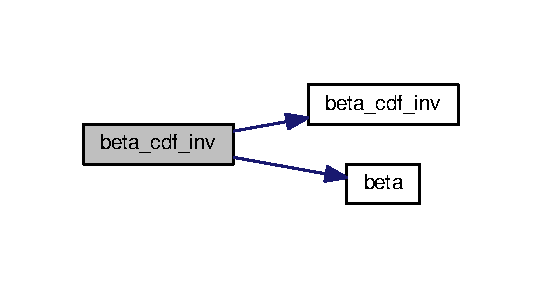
\includegraphics[width=260pt]{_bhabha__fortran__sem__doxy_8f_ad7b9df743251c691af6f3c722fc44a70_cgraph}
\end{center}
\end{figure}


\index{Bhabha\+\_\+fortran\+\_\+sem\+\_\+doxy.\+f@{Bhabha\+\_\+fortran\+\_\+sem\+\_\+doxy.\+f}!beta\+\_\+cdf\+\_\+inv\+\_\+old@{beta\+\_\+cdf\+\_\+inv\+\_\+old}}
\index{beta\+\_\+cdf\+\_\+inv\+\_\+old@{beta\+\_\+cdf\+\_\+inv\+\_\+old}!Bhabha\+\_\+fortran\+\_\+sem\+\_\+doxy.\+f@{Bhabha\+\_\+fortran\+\_\+sem\+\_\+doxy.\+f}}
\subsubsection[{\texorpdfstring{beta\+\_\+cdf\+\_\+inv\+\_\+old(cdf, a, b, x)}{beta_cdf_inv_old(cdf, a, b, x)}}]{\setlength{\rightskip}{0pt plus 5cm}subroutine beta\+\_\+cdf\+\_\+inv\+\_\+old (
\begin{DoxyParamCaption}
\item[{double precision, value}]{cdf, }
\item[{double precision}]{a, }
\item[{double precision}]{b, }
\item[{double precision}]{x}
\end{DoxyParamCaption}
)}\hypertarget{_bhabha__fortran__sem__doxy_8f_a809c02d9b3e29e164a314e6b82989080}{}\label{_bhabha__fortran__sem__doxy_8f_a809c02d9b3e29e164a314e6b82989080}


Definition at line 3124 of file Bhabha\+\_\+fortran\+\_\+sem\+\_\+doxy.\+f.



Here is the call graph for this function\+:\nopagebreak
\begin{figure}[H]
\begin{center}
\leavevmode
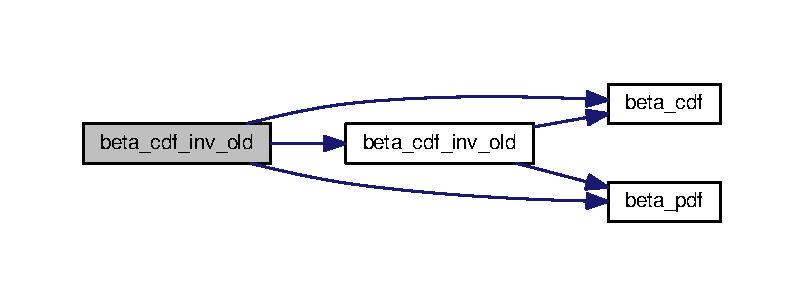
\includegraphics[width=350pt]{_bhabha__fortran__sem__doxy_8f_a809c02d9b3e29e164a314e6b82989080_cgraph}
\end{center}
\end{figure}


\index{Bhabha\+\_\+fortran\+\_\+sem\+\_\+doxy.\+f@{Bhabha\+\_\+fortran\+\_\+sem\+\_\+doxy.\+f}!beta\+\_\+cdf\+\_\+values@{beta\+\_\+cdf\+\_\+values}}
\index{beta\+\_\+cdf\+\_\+values@{beta\+\_\+cdf\+\_\+values}!Bhabha\+\_\+fortran\+\_\+sem\+\_\+doxy.\+f@{Bhabha\+\_\+fortran\+\_\+sem\+\_\+doxy.\+f}}
\subsubsection[{\texorpdfstring{beta\+\_\+cdf\+\_\+values(n\+\_\+data, a, b, x, fx)}{beta_cdf_values(n_data, a, b, x, fx)}}]{\setlength{\rightskip}{0pt plus 5cm}subroutine beta\+\_\+cdf\+\_\+values (
\begin{DoxyParamCaption}
\item[{integer, value}]{n\+\_\+data, }
\item[{double precision}]{a, }
\item[{double precision}]{b, }
\item[{double precision}]{x, }
\item[{double precision}]{fx}
\end{DoxyParamCaption}
)}\hypertarget{_bhabha__fortran__sem__doxy_8f_a6ca4d09928ee56be09ca34c70fbc37ce}{}\label{_bhabha__fortran__sem__doxy_8f_a6ca4d09928ee56be09ca34c70fbc37ce}


Definition at line 3285 of file Bhabha\+\_\+fortran\+\_\+sem\+\_\+doxy.\+f.



Here is the call graph for this function\+:\nopagebreak
\begin{figure}[H]
\begin{center}
\leavevmode
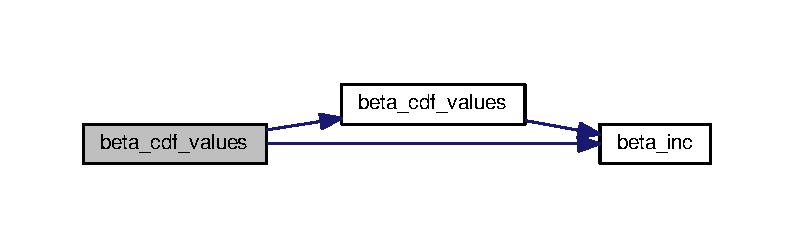
\includegraphics[width=350pt]{_bhabha__fortran__sem__doxy_8f_a6ca4d09928ee56be09ca34c70fbc37ce_cgraph}
\end{center}
\end{figure}


\index{Bhabha\+\_\+fortran\+\_\+sem\+\_\+doxy.\+f@{Bhabha\+\_\+fortran\+\_\+sem\+\_\+doxy.\+f}!beta\+\_\+check@{beta\+\_\+check}}
\index{beta\+\_\+check@{beta\+\_\+check}!Bhabha\+\_\+fortran\+\_\+sem\+\_\+doxy.\+f@{Bhabha\+\_\+fortran\+\_\+sem\+\_\+doxy.\+f}}
\subsubsection[{\texorpdfstring{beta\+\_\+check(a, b)}{beta_check(a, b)}}]{\setlength{\rightskip}{0pt plus 5cm}logical function beta\+\_\+check (
\begin{DoxyParamCaption}
\item[{double precision}]{a, }
\item[{double precision}]{b}
\end{DoxyParamCaption}
)}\hypertarget{_bhabha__fortran__sem__doxy_8f_a006a8a482ef44095ae5e65425badff73}{}\label{_bhabha__fortran__sem__doxy_8f_a006a8a482ef44095ae5e65425badff73}


Definition at line 3587 of file Bhabha\+\_\+fortran\+\_\+sem\+\_\+doxy.\+f.



Here is the call graph for this function\+:\nopagebreak
\begin{figure}[H]
\begin{center}
\leavevmode
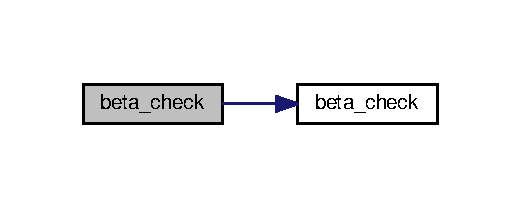
\includegraphics[width=250pt]{_bhabha__fortran__sem__doxy_8f_a006a8a482ef44095ae5e65425badff73_cgraph}
\end{center}
\end{figure}


\index{Bhabha\+\_\+fortran\+\_\+sem\+\_\+doxy.\+f@{Bhabha\+\_\+fortran\+\_\+sem\+\_\+doxy.\+f}!beta\+\_\+inc@{beta\+\_\+inc}}
\index{beta\+\_\+inc@{beta\+\_\+inc}!Bhabha\+\_\+fortran\+\_\+sem\+\_\+doxy.\+f@{Bhabha\+\_\+fortran\+\_\+sem\+\_\+doxy.\+f}}
\subsubsection[{\texorpdfstring{beta\+\_\+inc(a, b, x)}{beta_inc(a, b, x)}}]{\setlength{\rightskip}{0pt plus 5cm}double precision function beta\+\_\+inc (
\begin{DoxyParamCaption}
\item[{double precision}]{a, }
\item[{double precision}]{b, }
\item[{double precision}]{x}
\end{DoxyParamCaption}
)}\hypertarget{_bhabha__fortran__sem__doxy_8f_a2184970d382ccfa52654d945934a5db9}{}\label{_bhabha__fortran__sem__doxy_8f_a2184970d382ccfa52654d945934a5db9}


Definition at line 3639 of file Bhabha\+\_\+fortran\+\_\+sem\+\_\+doxy.\+f.



Here is the call graph for this function\+:\nopagebreak
\begin{figure}[H]
\begin{center}
\leavevmode
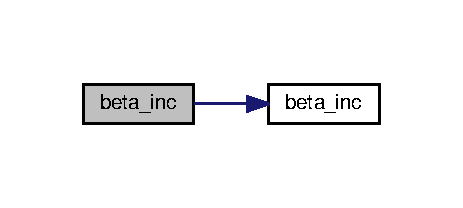
\includegraphics[width=222pt]{_bhabha__fortran__sem__doxy_8f_a2184970d382ccfa52654d945934a5db9_cgraph}
\end{center}
\end{figure}


\index{Bhabha\+\_\+fortran\+\_\+sem\+\_\+doxy.\+f@{Bhabha\+\_\+fortran\+\_\+sem\+\_\+doxy.\+f}!beta\+\_\+inc\+\_\+values@{beta\+\_\+inc\+\_\+values}}
\index{beta\+\_\+inc\+\_\+values@{beta\+\_\+inc\+\_\+values}!Bhabha\+\_\+fortran\+\_\+sem\+\_\+doxy.\+f@{Bhabha\+\_\+fortran\+\_\+sem\+\_\+doxy.\+f}}
\subsubsection[{\texorpdfstring{beta\+\_\+inc\+\_\+values(n\+\_\+data, a, b, x, fx)}{beta_inc_values(n_data, a, b, x, fx)}}]{\setlength{\rightskip}{0pt plus 5cm}subroutine beta\+\_\+inc\+\_\+values (
\begin{DoxyParamCaption}
\item[{integer, value}]{n\+\_\+data, }
\item[{double precision}]{a, }
\item[{double precision}]{b, }
\item[{double precision}]{x, }
\item[{double precision}]{fx}
\end{DoxyParamCaption}
)}\hypertarget{_bhabha__fortran__sem__doxy_8f_ad6f95398deb212fed550fff77fee8aa7}{}\label{_bhabha__fortran__sem__doxy_8f_ad6f95398deb212fed550fff77fee8aa7}


Definition at line 3820 of file Bhabha\+\_\+fortran\+\_\+sem\+\_\+doxy.\+f.



Here is the call graph for this function\+:\nopagebreak
\begin{figure}[H]
\begin{center}
\leavevmode
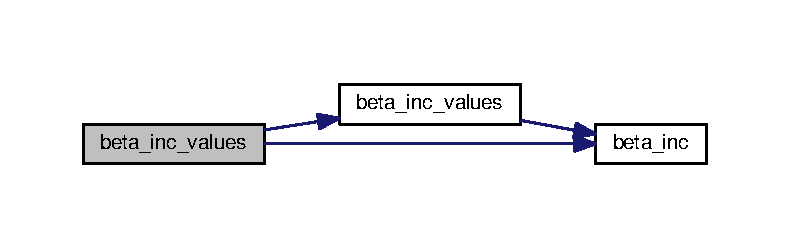
\includegraphics[width=350pt]{_bhabha__fortran__sem__doxy_8f_ad6f95398deb212fed550fff77fee8aa7_cgraph}
\end{center}
\end{figure}


\index{Bhabha\+\_\+fortran\+\_\+sem\+\_\+doxy.\+f@{Bhabha\+\_\+fortran\+\_\+sem\+\_\+doxy.\+f}!beta\+\_\+mean@{beta\+\_\+mean}}
\index{beta\+\_\+mean@{beta\+\_\+mean}!Bhabha\+\_\+fortran\+\_\+sem\+\_\+doxy.\+f@{Bhabha\+\_\+fortran\+\_\+sem\+\_\+doxy.\+f}}
\subsubsection[{\texorpdfstring{beta\+\_\+mean(a, b, mean)}{beta_mean(a, b, mean)}}]{\setlength{\rightskip}{0pt plus 5cm}subroutine beta\+\_\+mean (
\begin{DoxyParamCaption}
\item[{double precision}]{a, }
\item[{double precision}]{b, }
\item[{double precision}]{mean}
\end{DoxyParamCaption}
)}\hypertarget{_bhabha__fortran__sem__doxy_8f_a27758be0991a382242cea8fd6d1c6062}{}\label{_bhabha__fortran__sem__doxy_8f_a27758be0991a382242cea8fd6d1c6062}


Definition at line 4122 of file Bhabha\+\_\+fortran\+\_\+sem\+\_\+doxy.\+f.



Here is the call graph for this function\+:\nopagebreak
\begin{figure}[H]
\begin{center}
\leavevmode
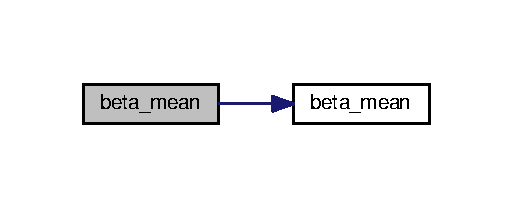
\includegraphics[width=246pt]{_bhabha__fortran__sem__doxy_8f_a27758be0991a382242cea8fd6d1c6062_cgraph}
\end{center}
\end{figure}


\index{Bhabha\+\_\+fortran\+\_\+sem\+\_\+doxy.\+f@{Bhabha\+\_\+fortran\+\_\+sem\+\_\+doxy.\+f}!beta\+\_\+pdf@{beta\+\_\+pdf}}
\index{beta\+\_\+pdf@{beta\+\_\+pdf}!Bhabha\+\_\+fortran\+\_\+sem\+\_\+doxy.\+f@{Bhabha\+\_\+fortran\+\_\+sem\+\_\+doxy.\+f}}
\subsubsection[{\texorpdfstring{beta\+\_\+pdf(x, a, b, pdf)}{beta_pdf(x, a, b, pdf)}}]{\setlength{\rightskip}{0pt plus 5cm}subroutine beta\+\_\+pdf (
\begin{DoxyParamCaption}
\item[{double precision}]{x, }
\item[{double precision}]{a, }
\item[{double precision}]{b, }
\item[{double precision, value}]{pdf}
\end{DoxyParamCaption}
)}\hypertarget{_bhabha__fortran__sem__doxy_8f_a98e50467dd638445b02798a39288af88}{}\label{_bhabha__fortran__sem__doxy_8f_a98e50467dd638445b02798a39288af88}


Definition at line 4158 of file Bhabha\+\_\+fortran\+\_\+sem\+\_\+doxy.\+f.



Here is the call graph for this function\+:\nopagebreak
\begin{figure}[H]
\begin{center}
\leavevmode
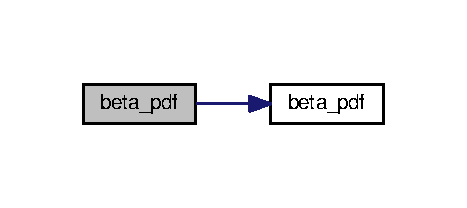
\includegraphics[width=224pt]{_bhabha__fortran__sem__doxy_8f_a98e50467dd638445b02798a39288af88_cgraph}
\end{center}
\end{figure}


\index{Bhabha\+\_\+fortran\+\_\+sem\+\_\+doxy.\+f@{Bhabha\+\_\+fortran\+\_\+sem\+\_\+doxy.\+f}!beta\+\_\+sample@{beta\+\_\+sample}}
\index{beta\+\_\+sample@{beta\+\_\+sample}!Bhabha\+\_\+fortran\+\_\+sem\+\_\+doxy.\+f@{Bhabha\+\_\+fortran\+\_\+sem\+\_\+doxy.\+f}}
\subsubsection[{\texorpdfstring{beta\+\_\+sample(a, b, seed, x)}{beta_sample(a, b, seed, x)}}]{\setlength{\rightskip}{0pt plus 5cm}subroutine beta\+\_\+sample (
\begin{DoxyParamCaption}
\item[{double precision}]{a, }
\item[{double precision}]{b, }
\item[{integer}]{seed, }
\item[{double precision}]{x}
\end{DoxyParamCaption}
)}\hypertarget{_bhabha__fortran__sem__doxy_8f_a4c2f42901cceca59466dde111153a465}{}\label{_bhabha__fortran__sem__doxy_8f_a4c2f42901cceca59466dde111153a465}


Definition at line 4215 of file Bhabha\+\_\+fortran\+\_\+sem\+\_\+doxy.\+f.



Here is the call graph for this function\+:\nopagebreak
\begin{figure}[H]
\begin{center}
\leavevmode
\includegraphics[width=260pt]{_bhabha__fortran__sem__doxy_8f_a4c2f42901cceca59466dde111153a465_cgraph}
\end{center}
\end{figure}


\index{Bhabha\+\_\+fortran\+\_\+sem\+\_\+doxy.\+f@{Bhabha\+\_\+fortran\+\_\+sem\+\_\+doxy.\+f}!beta\+\_\+variance@{beta\+\_\+variance}}
\index{beta\+\_\+variance@{beta\+\_\+variance}!Bhabha\+\_\+fortran\+\_\+sem\+\_\+doxy.\+f@{Bhabha\+\_\+fortran\+\_\+sem\+\_\+doxy.\+f}}
\subsubsection[{\texorpdfstring{beta\+\_\+variance(a, b, variance)}{beta_variance(a, b, variance)}}]{\setlength{\rightskip}{0pt plus 5cm}subroutine beta\+\_\+variance (
\begin{DoxyParamCaption}
\item[{double precision}]{a, }
\item[{double precision}]{b, }
\item[{double precision}]{variance}
\end{DoxyParamCaption}
)}\hypertarget{_bhabha__fortran__sem__doxy_8f_a646b52af6a87a1f9ad45365d12e84074}{}\label{_bhabha__fortran__sem__doxy_8f_a646b52af6a87a1f9ad45365d12e84074}


Definition at line 4295 of file Bhabha\+\_\+fortran\+\_\+sem\+\_\+doxy.\+f.



Here is the call graph for this function\+:\nopagebreak
\begin{figure}[H]
\begin{center}
\leavevmode
\includegraphics[width=270pt]{_bhabha__fortran__sem__doxy_8f_a646b52af6a87a1f9ad45365d12e84074_cgraph}
\end{center}
\end{figure}


\index{Bhabha\+\_\+fortran\+\_\+sem\+\_\+doxy.\+f@{Bhabha\+\_\+fortran\+\_\+sem\+\_\+doxy.\+f}!bhabha\+\_\+scattering@{bhabha\+\_\+scattering}}
\index{bhabha\+\_\+scattering@{bhabha\+\_\+scattering}!Bhabha\+\_\+fortran\+\_\+sem\+\_\+doxy.\+f@{Bhabha\+\_\+fortran\+\_\+sem\+\_\+doxy.\+f}}
\subsubsection[{\texorpdfstring{bhabha\+\_\+scattering}{bhabha_scattering}}]{\setlength{\rightskip}{0pt plus 5cm}program bhabha\+\_\+scattering (
\begin{DoxyParamCaption}
{}
\end{DoxyParamCaption}
)}\hypertarget{_bhabha__fortran__sem__doxy_8f_abb2a1b5ba16400d3f12a537f03a70349}{}\label{_bhabha__fortran__sem__doxy_8f_abb2a1b5ba16400d3f12a537f03a70349}


Definition at line 1 of file Bhabha\+\_\+fortran\+\_\+sem\+\_\+doxy.\+f.



Here is the call graph for this function\+:\nopagebreak
\begin{figure}[H]
\begin{center}
\leavevmode
\includegraphics[width=350pt]{_bhabha__fortran__sem__doxy_8f_abb2a1b5ba16400d3f12a537f03a70349_cgraph}
\end{center}
\end{figure}


\index{Bhabha\+\_\+fortran\+\_\+sem\+\_\+doxy.\+f@{Bhabha\+\_\+fortran\+\_\+sem\+\_\+doxy.\+f}!binomial\+\_\+cdf@{binomial\+\_\+cdf}}
\index{binomial\+\_\+cdf@{binomial\+\_\+cdf}!Bhabha\+\_\+fortran\+\_\+sem\+\_\+doxy.\+f@{Bhabha\+\_\+fortran\+\_\+sem\+\_\+doxy.\+f}}
\subsubsection[{\texorpdfstring{binomial\+\_\+cdf(x, a, b, cdf)}{binomial_cdf(x, a, b, cdf)}}]{\setlength{\rightskip}{0pt plus 5cm}subroutine binomial\+\_\+cdf (
\begin{DoxyParamCaption}
\item[{integer}]{x, }
\item[{integer}]{a, }
\item[{double precision}]{b, }
\item[{double precision, value}]{cdf}
\end{DoxyParamCaption}
)}\hypertarget{_bhabha__fortran__sem__doxy_8f_af7299d3fda796eea9a1be0c256f1624b}{}\label{_bhabha__fortran__sem__doxy_8f_af7299d3fda796eea9a1be0c256f1624b}


Definition at line 4331 of file Bhabha\+\_\+fortran\+\_\+sem\+\_\+doxy.\+f.



Here is the call graph for this function\+:\nopagebreak
\begin{figure}[H]
\begin{center}
\leavevmode
\includegraphics[width=258pt]{_bhabha__fortran__sem__doxy_8f_af7299d3fda796eea9a1be0c256f1624b_cgraph}
\end{center}
\end{figure}


\index{Bhabha\+\_\+fortran\+\_\+sem\+\_\+doxy.\+f@{Bhabha\+\_\+fortran\+\_\+sem\+\_\+doxy.\+f}!binomial\+\_\+cdf\+\_\+values@{binomial\+\_\+cdf\+\_\+values}}
\index{binomial\+\_\+cdf\+\_\+values@{binomial\+\_\+cdf\+\_\+values}!Bhabha\+\_\+fortran\+\_\+sem\+\_\+doxy.\+f@{Bhabha\+\_\+fortran\+\_\+sem\+\_\+doxy.\+f}}
\subsubsection[{\texorpdfstring{binomial\+\_\+cdf\+\_\+values(n\+\_\+data, a, b, x, fx)}{binomial_cdf_values(n_data, a, b, x, fx)}}]{\setlength{\rightskip}{0pt plus 5cm}subroutine binomial\+\_\+cdf\+\_\+values (
\begin{DoxyParamCaption}
\item[{integer, value}]{n\+\_\+data, }
\item[{}]{a, }
\item[{}]{b, }
\item[{integer}]{x, }
\item[{}]{fx}
\end{DoxyParamCaption}
)}\hypertarget{_bhabha__fortran__sem__doxy_8f_a8f4f3c2c05b8593455672a09762700d8}{}\label{_bhabha__fortran__sem__doxy_8f_a8f4f3c2c05b8593455672a09762700d8}


Definition at line 4414 of file Bhabha\+\_\+fortran\+\_\+sem\+\_\+doxy.\+f.



Here is the call graph for this function\+:\nopagebreak
\begin{figure}[H]
\begin{center}
\leavevmode
\includegraphics[width=326pt]{_bhabha__fortran__sem__doxy_8f_a8f4f3c2c05b8593455672a09762700d8_cgraph}
\end{center}
\end{figure}


\index{Bhabha\+\_\+fortran\+\_\+sem\+\_\+doxy.\+f@{Bhabha\+\_\+fortran\+\_\+sem\+\_\+doxy.\+f}!birthday\+\_\+cdf@{birthday\+\_\+cdf}}
\index{birthday\+\_\+cdf@{birthday\+\_\+cdf}!Bhabha\+\_\+fortran\+\_\+sem\+\_\+doxy.\+f@{Bhabha\+\_\+fortran\+\_\+sem\+\_\+doxy.\+f}}
\subsubsection[{\texorpdfstring{birthday\+\_\+cdf(n, cdf)}{birthday_cdf(n, cdf)}}]{\setlength{\rightskip}{0pt plus 5cm}subroutine birthday\+\_\+cdf (
\begin{DoxyParamCaption}
\item[{integer}]{n, }
\item[{double precision}]{cdf}
\end{DoxyParamCaption}
)}\hypertarget{_bhabha__fortran__sem__doxy_8f_a2ef757fb4d120a7339e7ba2d6e4df537}{}\label{_bhabha__fortran__sem__doxy_8f_a2ef757fb4d120a7339e7ba2d6e4df537}


Definition at line 1220 of file Bhabha\+\_\+fortran\+\_\+sem\+\_\+doxy.\+f.



Here is the call graph for this function\+:\nopagebreak
\begin{figure}[H]
\begin{center}
\leavevmode
\includegraphics[width=256pt]{_bhabha__fortran__sem__doxy_8f_a2ef757fb4d120a7339e7ba2d6e4df537_cgraph}
\end{center}
\end{figure}


\index{Bhabha\+\_\+fortran\+\_\+sem\+\_\+doxy.\+f@{Bhabha\+\_\+fortran\+\_\+sem\+\_\+doxy.\+f}!birthday\+\_\+cdf\+\_\+inv@{birthday\+\_\+cdf\+\_\+inv}}
\index{birthday\+\_\+cdf\+\_\+inv@{birthday\+\_\+cdf\+\_\+inv}!Bhabha\+\_\+fortran\+\_\+sem\+\_\+doxy.\+f@{Bhabha\+\_\+fortran\+\_\+sem\+\_\+doxy.\+f}}
\subsubsection[{\texorpdfstring{birthday\+\_\+cdf\+\_\+inv(cdf, n)}{birthday_cdf_inv(cdf, n)}}]{\setlength{\rightskip}{0pt plus 5cm}subroutine birthday\+\_\+cdf\+\_\+inv (
\begin{DoxyParamCaption}
\item[{double precision}]{cdf, }
\item[{integer}]{n}
\end{DoxyParamCaption}
)}\hypertarget{_bhabha__fortran__sem__doxy_8f_a8688523c630741866353afc455c7a5ee}{}\label{_bhabha__fortran__sem__doxy_8f_a8688523c630741866353afc455c7a5ee}


Definition at line 1276 of file Bhabha\+\_\+fortran\+\_\+sem\+\_\+doxy.\+f.



Here is the call graph for this function\+:\nopagebreak
\begin{figure}[H]
\begin{center}
\leavevmode
\includegraphics[width=292pt]{_bhabha__fortran__sem__doxy_8f_a8688523c630741866353afc455c7a5ee_cgraph}
\end{center}
\end{figure}


\index{Bhabha\+\_\+fortran\+\_\+sem\+\_\+doxy.\+f@{Bhabha\+\_\+fortran\+\_\+sem\+\_\+doxy.\+f}!birthday\+\_\+pdf@{birthday\+\_\+pdf}}
\index{birthday\+\_\+pdf@{birthday\+\_\+pdf}!Bhabha\+\_\+fortran\+\_\+sem\+\_\+doxy.\+f@{Bhabha\+\_\+fortran\+\_\+sem\+\_\+doxy.\+f}}
\subsubsection[{\texorpdfstring{birthday\+\_\+pdf(n, pdf)}{birthday_pdf(n, pdf)}}]{\setlength{\rightskip}{0pt plus 5cm}subroutine birthday\+\_\+pdf (
\begin{DoxyParamCaption}
\item[{integer}]{n, }
\item[{double precision}]{pdf}
\end{DoxyParamCaption}
)}\hypertarget{_bhabha__fortran__sem__doxy_8f_acae6886b34ec452abc19475c7905366b}{}\label{_bhabha__fortran__sem__doxy_8f_acae6886b34ec452abc19475c7905366b}


Definition at line 1333 of file Bhabha\+\_\+fortran\+\_\+sem\+\_\+doxy.\+f.



Here is the call graph for this function\+:\nopagebreak
\begin{figure}[H]
\begin{center}
\leavevmode
\includegraphics[width=256pt]{_bhabha__fortran__sem__doxy_8f_acae6886b34ec452abc19475c7905366b_cgraph}
\end{center}
\end{figure}


\index{Bhabha\+\_\+fortran\+\_\+sem\+\_\+doxy.\+f@{Bhabha\+\_\+fortran\+\_\+sem\+\_\+doxy.\+f}!chisquared@{chisquared}}
\index{chisquared@{chisquared}!Bhabha\+\_\+fortran\+\_\+sem\+\_\+doxy.\+f@{Bhabha\+\_\+fortran\+\_\+sem\+\_\+doxy.\+f}}
\subsubsection[{\texorpdfstring{chisquared(\+N, v, chi, chired, si2)}{chisquared(N, v, chi, chired, si2)}}]{\setlength{\rightskip}{0pt plus 5cm}subroutine chisquared (
\begin{DoxyParamCaption}
\item[{integer}]{N, }
\item[{integer}]{v, }
\item[{double precision}]{chi, }
\item[{double precision}]{chired, }
\item[{double precision}]{si2}
\end{DoxyParamCaption}
)}\hypertarget{_bhabha__fortran__sem__doxy_8f_a45708089271300abc165e88a11ab332e}{}\label{_bhabha__fortran__sem__doxy_8f_a45708089271300abc165e88a11ab332e}


Definition at line 102 of file Bhabha\+\_\+fortran\+\_\+sem\+\_\+doxy.\+f.



Here is the call graph for this function\+:\nopagebreak
\begin{figure}[H]
\begin{center}
\leavevmode
\includegraphics[width=233pt]{_bhabha__fortran__sem__doxy_8f_a45708089271300abc165e88a11ab332e_cgraph}
\end{center}
\end{figure}


\index{Bhabha\+\_\+fortran\+\_\+sem\+\_\+doxy.\+f@{Bhabha\+\_\+fortran\+\_\+sem\+\_\+doxy.\+f}!dsigma@{dsigma}}
\index{dsigma@{dsigma}!Bhabha\+\_\+fortran\+\_\+sem\+\_\+doxy.\+f@{Bhabha\+\_\+fortran\+\_\+sem\+\_\+doxy.\+f}}
\subsubsection[{\texorpdfstring{dsigma(\+S2, X)}{dsigma(S2, X)}}]{\setlength{\rightskip}{0pt plus 5cm}double precision function dsigma (
\begin{DoxyParamCaption}
\item[{double precision}]{S2, }
\item[{double precision}]{X}
\end{DoxyParamCaption}
)}\hypertarget{_bhabha__fortran__sem__doxy_8f_adb615d7a4a2665478c9f228d3281159e}{}\label{_bhabha__fortran__sem__doxy_8f_adb615d7a4a2665478c9f228d3281159e}


Definition at line 48 of file Bhabha\+\_\+fortran\+\_\+sem\+\_\+doxy.\+f.



Here is the call graph for this function\+:\nopagebreak
\begin{figure}[H]
\begin{center}
\leavevmode
\includegraphics[width=212pt]{_bhabha__fortran__sem__doxy_8f_adb615d7a4a2665478c9f228d3281159e_cgraph}
\end{center}
\end{figure}


\index{Bhabha\+\_\+fortran\+\_\+sem\+\_\+doxy.\+f@{Bhabha\+\_\+fortran\+\_\+sem\+\_\+doxy.\+f}!faux@{faux}}
\index{faux@{faux}!Bhabha\+\_\+fortran\+\_\+sem\+\_\+doxy.\+f@{Bhabha\+\_\+fortran\+\_\+sem\+\_\+doxy.\+f}}
\subsubsection[{\texorpdfstring{faux(\+X)}{faux(X)}}]{\setlength{\rightskip}{0pt plus 5cm}double precision function faux (
\begin{DoxyParamCaption}
\item[{double precision}]{X}
\end{DoxyParamCaption}
)}\hypertarget{_bhabha__fortran__sem__doxy_8f_a6ccd416a98c419022d77a6fc40b55868}{}\label{_bhabha__fortran__sem__doxy_8f_a6ccd416a98c419022d77a6fc40b55868}


Definition at line 76 of file Bhabha\+\_\+fortran\+\_\+sem\+\_\+doxy.\+f.

\index{Bhabha\+\_\+fortran\+\_\+sem\+\_\+doxy.\+f@{Bhabha\+\_\+fortran\+\_\+sem\+\_\+doxy.\+f}!geometric\+\_\+check@{geometric\+\_\+check}}
\index{geometric\+\_\+check@{geometric\+\_\+check}!Bhabha\+\_\+fortran\+\_\+sem\+\_\+doxy.\+f@{Bhabha\+\_\+fortran\+\_\+sem\+\_\+doxy.\+f}}
\subsubsection[{\texorpdfstring{geometric\+\_\+check(a)}{geometric_check(a)}}]{\setlength{\rightskip}{0pt plus 5cm}logical function geometric\+\_\+check (
\begin{DoxyParamCaption}
\item[{double precision}]{a}
\end{DoxyParamCaption}
)}\hypertarget{_bhabha__fortran__sem__doxy_8f_a5a9de1b5360cf06f54e5c25a475a9f34}{}\label{_bhabha__fortran__sem__doxy_8f_a5a9de1b5360cf06f54e5c25a475a9f34}


Definition at line 19120 of file Bhabha\+\_\+fortran\+\_\+sem\+\_\+doxy.\+f.



Here is the call graph for this function\+:\nopagebreak
\begin{figure}[H]
\begin{center}
\leavevmode
\includegraphics[width=298pt]{_bhabha__fortran__sem__doxy_8f_a5a9de1b5360cf06f54e5c25a475a9f34_cgraph}
\end{center}
\end{figure}


\index{Bhabha\+\_\+fortran\+\_\+sem\+\_\+doxy.\+f@{Bhabha\+\_\+fortran\+\_\+sem\+\_\+doxy.\+f}!geometric\+\_\+mean@{geometric\+\_\+mean}}
\index{geometric\+\_\+mean@{geometric\+\_\+mean}!Bhabha\+\_\+fortran\+\_\+sem\+\_\+doxy.\+f@{Bhabha\+\_\+fortran\+\_\+sem\+\_\+doxy.\+f}}
\subsubsection[{\texorpdfstring{geometric\+\_\+mean(a, mean)}{geometric_mean(a, mean)}}]{\setlength{\rightskip}{0pt plus 5cm}subroutine geometric\+\_\+mean (
\begin{DoxyParamCaption}
\item[{double precision}]{a, }
\item[{double precision}]{mean}
\end{DoxyParamCaption}
)}\hypertarget{_bhabha__fortran__sem__doxy_8f_a1ffa752cfa7e58c775d58ebf3ddff183}{}\label{_bhabha__fortran__sem__doxy_8f_a1ffa752cfa7e58c775d58ebf3ddff183}


Definition at line 19162 of file Bhabha\+\_\+fortran\+\_\+sem\+\_\+doxy.\+f.



Here is the call graph for this function\+:\nopagebreak
\begin{figure}[H]
\begin{center}
\leavevmode
\includegraphics[width=294pt]{_bhabha__fortran__sem__doxy_8f_a1ffa752cfa7e58c775d58ebf3ddff183_cgraph}
\end{center}
\end{figure}


\index{Bhabha\+\_\+fortran\+\_\+sem\+\_\+doxy.\+f@{Bhabha\+\_\+fortran\+\_\+sem\+\_\+doxy.\+f}!geometric\+\_\+pdf@{geometric\+\_\+pdf}}
\index{geometric\+\_\+pdf@{geometric\+\_\+pdf}!Bhabha\+\_\+fortran\+\_\+sem\+\_\+doxy.\+f@{Bhabha\+\_\+fortran\+\_\+sem\+\_\+doxy.\+f}}
\subsubsection[{\texorpdfstring{geometric\+\_\+pdf(x, a, pdf)}{geometric_pdf(x, a, pdf)}}]{\setlength{\rightskip}{0pt plus 5cm}subroutine geometric\+\_\+pdf (
\begin{DoxyParamCaption}
\item[{integer}]{x, }
\item[{double precision}]{a, }
\item[{double precision, value}]{pdf}
\end{DoxyParamCaption}
)}\hypertarget{_bhabha__fortran__sem__doxy_8f_ad7c75816231cf277056551ca6c56d50d}{}\label{_bhabha__fortran__sem__doxy_8f_ad7c75816231cf277056551ca6c56d50d}


Definition at line 19201 of file Bhabha\+\_\+fortran\+\_\+sem\+\_\+doxy.\+f.



Here is the call graph for this function\+:\nopagebreak
\begin{figure}[H]
\begin{center}
\leavevmode
\includegraphics[width=272pt]{_bhabha__fortran__sem__doxy_8f_ad7c75816231cf277056551ca6c56d50d_cgraph}
\end{center}
\end{figure}


\index{Bhabha\+\_\+fortran\+\_\+sem\+\_\+doxy.\+f@{Bhabha\+\_\+fortran\+\_\+sem\+\_\+doxy.\+f}!geometric\+\_\+sample@{geometric\+\_\+sample}}
\index{geometric\+\_\+sample@{geometric\+\_\+sample}!Bhabha\+\_\+fortran\+\_\+sem\+\_\+doxy.\+f@{Bhabha\+\_\+fortran\+\_\+sem\+\_\+doxy.\+f}}
\subsubsection[{\texorpdfstring{geometric\+\_\+sample(a, seed, x)}{geometric_sample(a, seed, x)}}]{\setlength{\rightskip}{0pt plus 5cm}subroutine geometric\+\_\+sample (
\begin{DoxyParamCaption}
\item[{double precision}]{a, }
\item[{integer}]{seed, }
\item[{integer}]{x}
\end{DoxyParamCaption}
)}\hypertarget{_bhabha__fortran__sem__doxy_8f_a8e9806974aa07e008b7027a4d4fccca8}{}\label{_bhabha__fortran__sem__doxy_8f_a8e9806974aa07e008b7027a4d4fccca8}


Definition at line 19269 of file Bhabha\+\_\+fortran\+\_\+sem\+\_\+doxy.\+f.



Here is the call graph for this function\+:\nopagebreak
\begin{figure}[H]
\begin{center}
\leavevmode
\includegraphics[width=308pt]{_bhabha__fortran__sem__doxy_8f_a8e9806974aa07e008b7027a4d4fccca8_cgraph}
\end{center}
\end{figure}


\index{Bhabha\+\_\+fortran\+\_\+sem\+\_\+doxy.\+f@{Bhabha\+\_\+fortran\+\_\+sem\+\_\+doxy.\+f}!geometric\+\_\+variance@{geometric\+\_\+variance}}
\index{geometric\+\_\+variance@{geometric\+\_\+variance}!Bhabha\+\_\+fortran\+\_\+sem\+\_\+doxy.\+f@{Bhabha\+\_\+fortran\+\_\+sem\+\_\+doxy.\+f}}
\subsubsection[{\texorpdfstring{geometric\+\_\+variance(a, variance)}{geometric_variance(a, variance)}}]{\setlength{\rightskip}{0pt plus 5cm}subroutine geometric\+\_\+variance (
\begin{DoxyParamCaption}
\item[{double precision}]{a, }
\item[{double precision}]{variance}
\end{DoxyParamCaption}
)}\hypertarget{_bhabha__fortran__sem__doxy_8f_ae112b39e2f8d5468f1f366cc8e3afd90}{}\label{_bhabha__fortran__sem__doxy_8f_ae112b39e2f8d5468f1f366cc8e3afd90}


Definition at line 19311 of file Bhabha\+\_\+fortran\+\_\+sem\+\_\+doxy.\+f.



Here is the call graph for this function\+:\nopagebreak
\begin{figure}[H]
\begin{center}
\leavevmode
\includegraphics[width=318pt]{_bhabha__fortran__sem__doxy_8f_ae112b39e2f8d5468f1f366cc8e3afd90_cgraph}
\end{center}
\end{figure}


\index{Bhabha\+\_\+fortran\+\_\+sem\+\_\+doxy.\+f@{Bhabha\+\_\+fortran\+\_\+sem\+\_\+doxy.\+f}!gompertz\+\_\+cdf@{gompertz\+\_\+cdf}}
\index{gompertz\+\_\+cdf@{gompertz\+\_\+cdf}!Bhabha\+\_\+fortran\+\_\+sem\+\_\+doxy.\+f@{Bhabha\+\_\+fortran\+\_\+sem\+\_\+doxy.\+f}}
\subsubsection[{\texorpdfstring{gompertz\+\_\+cdf(x, a, b, cdf)}{gompertz_cdf(x, a, b, cdf)}}]{\setlength{\rightskip}{0pt plus 5cm}subroutine gompertz\+\_\+cdf (
\begin{DoxyParamCaption}
\item[{double precision}]{x, }
\item[{double precision}]{a, }
\item[{double precision}]{b, }
\item[{double precision, value}]{cdf}
\end{DoxyParamCaption}
)}\hypertarget{_bhabha__fortran__sem__doxy_8f_af902e014759d310f9104881f90934632}{}\label{_bhabha__fortran__sem__doxy_8f_af902e014759d310f9104881f90934632}


Definition at line 19345 of file Bhabha\+\_\+fortran\+\_\+sem\+\_\+doxy.\+f.



Here is the call graph for this function\+:\nopagebreak
\begin{figure}[H]
\begin{center}
\leavevmode
\includegraphics[width=268pt]{_bhabha__fortran__sem__doxy_8f_af902e014759d310f9104881f90934632_cgraph}
\end{center}
\end{figure}


\index{Bhabha\+\_\+fortran\+\_\+sem\+\_\+doxy.\+f@{Bhabha\+\_\+fortran\+\_\+sem\+\_\+doxy.\+f}!gompertz\+\_\+cdf\+\_\+inv@{gompertz\+\_\+cdf\+\_\+inv}}
\index{gompertz\+\_\+cdf\+\_\+inv@{gompertz\+\_\+cdf\+\_\+inv}!Bhabha\+\_\+fortran\+\_\+sem\+\_\+doxy.\+f@{Bhabha\+\_\+fortran\+\_\+sem\+\_\+doxy.\+f}}
\subsubsection[{\texorpdfstring{gompertz\+\_\+cdf\+\_\+inv(cdf, a, b, x)}{gompertz_cdf_inv(cdf, a, b, x)}}]{\setlength{\rightskip}{0pt plus 5cm}subroutine gompertz\+\_\+cdf\+\_\+inv (
\begin{DoxyParamCaption}
\item[{double precision, value}]{cdf, }
\item[{double precision}]{a, }
\item[{double precision}]{b, }
\item[{double precision}]{x}
\end{DoxyParamCaption}
)}\hypertarget{_bhabha__fortran__sem__doxy_8f_aca5ab8f72105aabb509bd487e8c8b6e6}{}\label{_bhabha__fortran__sem__doxy_8f_aca5ab8f72105aabb509bd487e8c8b6e6}


Definition at line 19394 of file Bhabha\+\_\+fortran\+\_\+sem\+\_\+doxy.\+f.



Here is the call graph for this function\+:\nopagebreak
\begin{figure}[H]
\begin{center}
\leavevmode
\includegraphics[width=304pt]{_bhabha__fortran__sem__doxy_8f_aca5ab8f72105aabb509bd487e8c8b6e6_cgraph}
\end{center}
\end{figure}


\index{Bhabha\+\_\+fortran\+\_\+sem\+\_\+doxy.\+f@{Bhabha\+\_\+fortran\+\_\+sem\+\_\+doxy.\+f}!gompertz\+\_\+check@{gompertz\+\_\+check}}
\index{gompertz\+\_\+check@{gompertz\+\_\+check}!Bhabha\+\_\+fortran\+\_\+sem\+\_\+doxy.\+f@{Bhabha\+\_\+fortran\+\_\+sem\+\_\+doxy.\+f}}
\subsubsection[{\texorpdfstring{gompertz\+\_\+check(a, b)}{gompertz_check(a, b)}}]{\setlength{\rightskip}{0pt plus 5cm}logical function gompertz\+\_\+check (
\begin{DoxyParamCaption}
\item[{double precision}]{a, }
\item[{double precision}]{b}
\end{DoxyParamCaption}
)}\hypertarget{_bhabha__fortran__sem__doxy_8f_a6dcecb2ef74b499aa1313117cb5bf666}{}\label{_bhabha__fortran__sem__doxy_8f_a6dcecb2ef74b499aa1313117cb5bf666}


Definition at line 19452 of file Bhabha\+\_\+fortran\+\_\+sem\+\_\+doxy.\+f.



Here is the call graph for this function\+:\nopagebreak
\begin{figure}[H]
\begin{center}
\leavevmode
\includegraphics[width=294pt]{_bhabha__fortran__sem__doxy_8f_a6dcecb2ef74b499aa1313117cb5bf666_cgraph}
\end{center}
\end{figure}


\index{Bhabha\+\_\+fortran\+\_\+sem\+\_\+doxy.\+f@{Bhabha\+\_\+fortran\+\_\+sem\+\_\+doxy.\+f}!gompertz\+\_\+pdf@{gompertz\+\_\+pdf}}
\index{gompertz\+\_\+pdf@{gompertz\+\_\+pdf}!Bhabha\+\_\+fortran\+\_\+sem\+\_\+doxy.\+f@{Bhabha\+\_\+fortran\+\_\+sem\+\_\+doxy.\+f}}
\subsubsection[{\texorpdfstring{gompertz\+\_\+pdf(x, a, b, pdf)}{gompertz_pdf(x, a, b, pdf)}}]{\setlength{\rightskip}{0pt plus 5cm}subroutine gompertz\+\_\+pdf (
\begin{DoxyParamCaption}
\item[{double precision}]{x, }
\item[{double precision}]{a, }
\item[{double precision}]{b, }
\item[{double precision, value}]{pdf}
\end{DoxyParamCaption}
)}\hypertarget{_bhabha__fortran__sem__doxy_8f_ad1b796cd8b7d10dc0096cf2a42b748be}{}\label{_bhabha__fortran__sem__doxy_8f_ad1b796cd8b7d10dc0096cf2a42b748be}


Definition at line 19510 of file Bhabha\+\_\+fortran\+\_\+sem\+\_\+doxy.\+f.



Here is the call graph for this function\+:\nopagebreak
\begin{figure}[H]
\begin{center}
\leavevmode
\includegraphics[width=268pt]{_bhabha__fortran__sem__doxy_8f_ad1b796cd8b7d10dc0096cf2a42b748be_cgraph}
\end{center}
\end{figure}


\index{Bhabha\+\_\+fortran\+\_\+sem\+\_\+doxy.\+f@{Bhabha\+\_\+fortran\+\_\+sem\+\_\+doxy.\+f}!gompertz\+\_\+sample@{gompertz\+\_\+sample}}
\index{gompertz\+\_\+sample@{gompertz\+\_\+sample}!Bhabha\+\_\+fortran\+\_\+sem\+\_\+doxy.\+f@{Bhabha\+\_\+fortran\+\_\+sem\+\_\+doxy.\+f}}
\subsubsection[{\texorpdfstring{gompertz\+\_\+sample(a, b, seed, x)}{gompertz_sample(a, b, seed, x)}}]{\setlength{\rightskip}{0pt plus 5cm}subroutine gompertz\+\_\+sample (
\begin{DoxyParamCaption}
\item[{double precision}]{a, }
\item[{double precision}]{b, }
\item[{integer}]{seed, }
\item[{double precision}]{x}
\end{DoxyParamCaption}
)}\hypertarget{_bhabha__fortran__sem__doxy_8f_adee76c73484194b0ddb1c677c0d03407}{}\label{_bhabha__fortran__sem__doxy_8f_adee76c73484194b0ddb1c677c0d03407}


Definition at line 19574 of file Bhabha\+\_\+fortran\+\_\+sem\+\_\+doxy.\+f.



Here is the call graph for this function\+:\nopagebreak
\begin{figure}[H]
\begin{center}
\leavevmode
\includegraphics[width=350pt]{_bhabha__fortran__sem__doxy_8f_adee76c73484194b0ddb1c677c0d03407_cgraph}
\end{center}
\end{figure}


\index{Bhabha\+\_\+fortran\+\_\+sem\+\_\+doxy.\+f@{Bhabha\+\_\+fortran\+\_\+sem\+\_\+doxy.\+f}!gumbel\+\_\+cdf@{gumbel\+\_\+cdf}}
\index{gumbel\+\_\+cdf@{gumbel\+\_\+cdf}!Bhabha\+\_\+fortran\+\_\+sem\+\_\+doxy.\+f@{Bhabha\+\_\+fortran\+\_\+sem\+\_\+doxy.\+f}}
\subsubsection[{\texorpdfstring{gumbel\+\_\+cdf(x, cdf)}{gumbel_cdf(x, cdf)}}]{\setlength{\rightskip}{0pt plus 5cm}subroutine gumbel\+\_\+cdf (
\begin{DoxyParamCaption}
\item[{double precision}]{x, }
\item[{double precision, value}]{cdf}
\end{DoxyParamCaption}
)}\hypertarget{_bhabha__fortran__sem__doxy_8f_a3406fe8568d2dfb52a66cc4470893365}{}\label{_bhabha__fortran__sem__doxy_8f_a3406fe8568d2dfb52a66cc4470893365}


Definition at line 19617 of file Bhabha\+\_\+fortran\+\_\+sem\+\_\+doxy.\+f.



Here is the call graph for this function\+:\nopagebreak
\begin{figure}[H]
\begin{center}
\leavevmode
\includegraphics[width=250pt]{_bhabha__fortran__sem__doxy_8f_a3406fe8568d2dfb52a66cc4470893365_cgraph}
\end{center}
\end{figure}


\index{Bhabha\+\_\+fortran\+\_\+sem\+\_\+doxy.\+f@{Bhabha\+\_\+fortran\+\_\+sem\+\_\+doxy.\+f}!gumbel\+\_\+cdf\+\_\+inv@{gumbel\+\_\+cdf\+\_\+inv}}
\index{gumbel\+\_\+cdf\+\_\+inv@{gumbel\+\_\+cdf\+\_\+inv}!Bhabha\+\_\+fortran\+\_\+sem\+\_\+doxy.\+f@{Bhabha\+\_\+fortran\+\_\+sem\+\_\+doxy.\+f}}
\subsubsection[{\texorpdfstring{gumbel\+\_\+cdf\+\_\+inv(cdf, x)}{gumbel_cdf_inv(cdf, x)}}]{\setlength{\rightskip}{0pt plus 5cm}subroutine gumbel\+\_\+cdf\+\_\+inv (
\begin{DoxyParamCaption}
\item[{double precision, value}]{cdf, }
\item[{double precision}]{x}
\end{DoxyParamCaption}
)}\hypertarget{_bhabha__fortran__sem__doxy_8f_af645551cd94f4f929966f33fade3bb03}{}\label{_bhabha__fortran__sem__doxy_8f_af645551cd94f4f929966f33fade3bb03}


Definition at line 19650 of file Bhabha\+\_\+fortran\+\_\+sem\+\_\+doxy.\+f.



Here is the call graph for this function\+:\nopagebreak
\begin{figure}[H]
\begin{center}
\leavevmode
\includegraphics[width=286pt]{_bhabha__fortran__sem__doxy_8f_af645551cd94f4f929966f33fade3bb03_cgraph}
\end{center}
\end{figure}


\index{Bhabha\+\_\+fortran\+\_\+sem\+\_\+doxy.\+f@{Bhabha\+\_\+fortran\+\_\+sem\+\_\+doxy.\+f}!gumbel\+\_\+mean@{gumbel\+\_\+mean}}
\index{gumbel\+\_\+mean@{gumbel\+\_\+mean}!Bhabha\+\_\+fortran\+\_\+sem\+\_\+doxy.\+f@{Bhabha\+\_\+fortran\+\_\+sem\+\_\+doxy.\+f}}
\subsubsection[{\texorpdfstring{gumbel\+\_\+mean(mean)}{gumbel_mean(mean)}}]{\setlength{\rightskip}{0pt plus 5cm}subroutine gumbel\+\_\+mean (
\begin{DoxyParamCaption}
\item[{double precision}]{mean}
\end{DoxyParamCaption}
)}\hypertarget{_bhabha__fortran__sem__doxy_8f_ab25784871afe33475733991e2db8c754}{}\label{_bhabha__fortran__sem__doxy_8f_ab25784871afe33475733991e2db8c754}


Definition at line 19691 of file Bhabha\+\_\+fortran\+\_\+sem\+\_\+doxy.\+f.



Here is the call graph for this function\+:\nopagebreak
\begin{figure}[H]
\begin{center}
\leavevmode
\includegraphics[width=270pt]{_bhabha__fortran__sem__doxy_8f_ab25784871afe33475733991e2db8c754_cgraph}
\end{center}
\end{figure}


\index{Bhabha\+\_\+fortran\+\_\+sem\+\_\+doxy.\+f@{Bhabha\+\_\+fortran\+\_\+sem\+\_\+doxy.\+f}!gumbel\+\_\+pdf@{gumbel\+\_\+pdf}}
\index{gumbel\+\_\+pdf@{gumbel\+\_\+pdf}!Bhabha\+\_\+fortran\+\_\+sem\+\_\+doxy.\+f@{Bhabha\+\_\+fortran\+\_\+sem\+\_\+doxy.\+f}}
\subsubsection[{\texorpdfstring{gumbel\+\_\+pdf(x, pdf)}{gumbel_pdf(x, pdf)}}]{\setlength{\rightskip}{0pt plus 5cm}subroutine gumbel\+\_\+pdf (
\begin{DoxyParamCaption}
\item[{double precision}]{x, }
\item[{double precision, value}]{pdf}
\end{DoxyParamCaption}
)}\hypertarget{_bhabha__fortran__sem__doxy_8f_a6d2003af12b56d5f9b0a816e24b5775c}{}\label{_bhabha__fortran__sem__doxy_8f_a6d2003af12b56d5f9b0a816e24b5775c}


Definition at line 19722 of file Bhabha\+\_\+fortran\+\_\+sem\+\_\+doxy.\+f.



Here is the call graph for this function\+:\nopagebreak
\begin{figure}[H]
\begin{center}
\leavevmode
\includegraphics[width=250pt]{_bhabha__fortran__sem__doxy_8f_a6d2003af12b56d5f9b0a816e24b5775c_cgraph}
\end{center}
\end{figure}


\index{Bhabha\+\_\+fortran\+\_\+sem\+\_\+doxy.\+f@{Bhabha\+\_\+fortran\+\_\+sem\+\_\+doxy.\+f}!gumbel\+\_\+sample@{gumbel\+\_\+sample}}
\index{gumbel\+\_\+sample@{gumbel\+\_\+sample}!Bhabha\+\_\+fortran\+\_\+sem\+\_\+doxy.\+f@{Bhabha\+\_\+fortran\+\_\+sem\+\_\+doxy.\+f}}
\subsubsection[{\texorpdfstring{gumbel\+\_\+sample(seed, x)}{gumbel_sample(seed, x)}}]{\setlength{\rightskip}{0pt plus 5cm}subroutine gumbel\+\_\+sample (
\begin{DoxyParamCaption}
\item[{integer}]{seed, }
\item[{double precision}]{x}
\end{DoxyParamCaption}
)}\hypertarget{_bhabha__fortran__sem__doxy_8f_a4eda1bafea5a35dad5e4d1f3c7c4c2fd}{}\label{_bhabha__fortran__sem__doxy_8f_a4eda1bafea5a35dad5e4d1f3c7c4c2fd}


Definition at line 19767 of file Bhabha\+\_\+fortran\+\_\+sem\+\_\+doxy.\+f.



Here is the call graph for this function\+:\nopagebreak
\begin{figure}[H]
\begin{center}
\leavevmode
\includegraphics[width=350pt]{_bhabha__fortran__sem__doxy_8f_a4eda1bafea5a35dad5e4d1f3c7c4c2fd_cgraph}
\end{center}
\end{figure}


\index{Bhabha\+\_\+fortran\+\_\+sem\+\_\+doxy.\+f@{Bhabha\+\_\+fortran\+\_\+sem\+\_\+doxy.\+f}!gumbel\+\_\+variance@{gumbel\+\_\+variance}}
\index{gumbel\+\_\+variance@{gumbel\+\_\+variance}!Bhabha\+\_\+fortran\+\_\+sem\+\_\+doxy.\+f@{Bhabha\+\_\+fortran\+\_\+sem\+\_\+doxy.\+f}}
\subsubsection[{\texorpdfstring{gumbel\+\_\+variance(variance)}{gumbel_variance(variance)}}]{\setlength{\rightskip}{0pt plus 5cm}subroutine gumbel\+\_\+variance (
\begin{DoxyParamCaption}
\item[{double precision}]{variance}
\end{DoxyParamCaption}
)}\hypertarget{_bhabha__fortran__sem__doxy_8f_a0b9d97396f3f7a256ac7b587d8bf44d0}{}\label{_bhabha__fortran__sem__doxy_8f_a0b9d97396f3f7a256ac7b587d8bf44d0}


Definition at line 19805 of file Bhabha\+\_\+fortran\+\_\+sem\+\_\+doxy.\+f.



Here is the call graph for this function\+:\nopagebreak
\begin{figure}[H]
\begin{center}
\leavevmode
\includegraphics[width=296pt]{_bhabha__fortran__sem__doxy_8f_a0b9d97396f3f7a256ac7b587d8bf44d0_cgraph}
\end{center}
\end{figure}


\index{Bhabha\+\_\+fortran\+\_\+sem\+\_\+doxy.\+f@{Bhabha\+\_\+fortran\+\_\+sem\+\_\+doxy.\+f}!half\+\_\+normal\+\_\+cdf@{half\+\_\+normal\+\_\+cdf}}
\index{half\+\_\+normal\+\_\+cdf@{half\+\_\+normal\+\_\+cdf}!Bhabha\+\_\+fortran\+\_\+sem\+\_\+doxy.\+f@{Bhabha\+\_\+fortran\+\_\+sem\+\_\+doxy.\+f}}
\subsubsection[{\texorpdfstring{half\+\_\+normal\+\_\+cdf(x, a, b, cdf)}{half_normal_cdf(x, a, b, cdf)}}]{\setlength{\rightskip}{0pt plus 5cm}subroutine half\+\_\+normal\+\_\+cdf (
\begin{DoxyParamCaption}
\item[{double precision}]{x, }
\item[{double precision}]{a, }
\item[{double precision}]{b, }
\item[{double precision, value}]{cdf}
\end{DoxyParamCaption}
)}\hypertarget{_bhabha__fortran__sem__doxy_8f_a151eb67716499cd4c2674750d365bbda}{}\label{_bhabha__fortran__sem__doxy_8f_a151eb67716499cd4c2674750d365bbda}


Definition at line 19837 of file Bhabha\+\_\+fortran\+\_\+sem\+\_\+doxy.\+f.



Here is the call graph for this function\+:\nopagebreak
\begin{figure}[H]
\begin{center}
\leavevmode
\includegraphics[width=288pt]{_bhabha__fortran__sem__doxy_8f_a151eb67716499cd4c2674750d365bbda_cgraph}
\end{center}
\end{figure}


\index{Bhabha\+\_\+fortran\+\_\+sem\+\_\+doxy.\+f@{Bhabha\+\_\+fortran\+\_\+sem\+\_\+doxy.\+f}!half\+\_\+normal\+\_\+cdf\+\_\+inv@{half\+\_\+normal\+\_\+cdf\+\_\+inv}}
\index{half\+\_\+normal\+\_\+cdf\+\_\+inv@{half\+\_\+normal\+\_\+cdf\+\_\+inv}!Bhabha\+\_\+fortran\+\_\+sem\+\_\+doxy.\+f@{Bhabha\+\_\+fortran\+\_\+sem\+\_\+doxy.\+f}}
\subsubsection[{\texorpdfstring{half\+\_\+normal\+\_\+cdf\+\_\+inv(cdf, a, b, x)}{half_normal_cdf_inv(cdf, a, b, x)}}]{\setlength{\rightskip}{0pt plus 5cm}subroutine half\+\_\+normal\+\_\+cdf\+\_\+inv (
\begin{DoxyParamCaption}
\item[{double precision, value}]{cdf, }
\item[{double precision}]{a, }
\item[{double precision}]{b, }
\item[{double precision}]{x}
\end{DoxyParamCaption}
)}\hypertarget{_bhabha__fortran__sem__doxy_8f_ab3ab8dee9a6bab9e5f838055b6a15e32}{}\label{_bhabha__fortran__sem__doxy_8f_ab3ab8dee9a6bab9e5f838055b6a15e32}


Definition at line 19881 of file Bhabha\+\_\+fortran\+\_\+sem\+\_\+doxy.\+f.



Here is the call graph for this function\+:\nopagebreak
\begin{figure}[H]
\begin{center}
\leavevmode
\includegraphics[width=324pt]{_bhabha__fortran__sem__doxy_8f_ab3ab8dee9a6bab9e5f838055b6a15e32_cgraph}
\end{center}
\end{figure}


\index{Bhabha\+\_\+fortran\+\_\+sem\+\_\+doxy.\+f@{Bhabha\+\_\+fortran\+\_\+sem\+\_\+doxy.\+f}!half\+\_\+normal\+\_\+check@{half\+\_\+normal\+\_\+check}}
\index{half\+\_\+normal\+\_\+check@{half\+\_\+normal\+\_\+check}!Bhabha\+\_\+fortran\+\_\+sem\+\_\+doxy.\+f@{Bhabha\+\_\+fortran\+\_\+sem\+\_\+doxy.\+f}}
\subsubsection[{\texorpdfstring{half\+\_\+normal\+\_\+check(a, b)}{half_normal_check(a, b)}}]{\setlength{\rightskip}{0pt plus 5cm}logical function half\+\_\+normal\+\_\+check (
\begin{DoxyParamCaption}
\item[{double precision}]{a, }
\item[{double precision}]{b}
\end{DoxyParamCaption}
)}\hypertarget{_bhabha__fortran__sem__doxy_8f_aff12e14edd4bf669955f0a594154edf8}{}\label{_bhabha__fortran__sem__doxy_8f_aff12e14edd4bf669955f0a594154edf8}


Definition at line 19930 of file Bhabha\+\_\+fortran\+\_\+sem\+\_\+doxy.\+f.



Here is the call graph for this function\+:\nopagebreak
\begin{figure}[H]
\begin{center}
\leavevmode
\includegraphics[width=312pt]{_bhabha__fortran__sem__doxy_8f_aff12e14edd4bf669955f0a594154edf8_cgraph}
\end{center}
\end{figure}


\index{Bhabha\+\_\+fortran\+\_\+sem\+\_\+doxy.\+f@{Bhabha\+\_\+fortran\+\_\+sem\+\_\+doxy.\+f}!half\+\_\+normal\+\_\+mean@{half\+\_\+normal\+\_\+mean}}
\index{half\+\_\+normal\+\_\+mean@{half\+\_\+normal\+\_\+mean}!Bhabha\+\_\+fortran\+\_\+sem\+\_\+doxy.\+f@{Bhabha\+\_\+fortran\+\_\+sem\+\_\+doxy.\+f}}
\subsubsection[{\texorpdfstring{half\+\_\+normal\+\_\+mean(a, b, mean)}{half_normal_mean(a, b, mean)}}]{\setlength{\rightskip}{0pt plus 5cm}subroutine half\+\_\+normal\+\_\+mean (
\begin{DoxyParamCaption}
\item[{double precision}]{a, }
\item[{double precision}]{b, }
\item[{double precision}]{mean}
\end{DoxyParamCaption}
)}\hypertarget{_bhabha__fortran__sem__doxy_8f_a113c46e78879c405f2eac9a5ffc6df15}{}\label{_bhabha__fortran__sem__doxy_8f_a113c46e78879c405f2eac9a5ffc6df15}


Definition at line 19973 of file Bhabha\+\_\+fortran\+\_\+sem\+\_\+doxy.\+f.



Here is the call graph for this function\+:\nopagebreak
\begin{figure}[H]
\begin{center}
\leavevmode
\includegraphics[width=308pt]{_bhabha__fortran__sem__doxy_8f_a113c46e78879c405f2eac9a5ffc6df15_cgraph}
\end{center}
\end{figure}


\index{Bhabha\+\_\+fortran\+\_\+sem\+\_\+doxy.\+f@{Bhabha\+\_\+fortran\+\_\+sem\+\_\+doxy.\+f}!half\+\_\+normal\+\_\+pdf@{half\+\_\+normal\+\_\+pdf}}
\index{half\+\_\+normal\+\_\+pdf@{half\+\_\+normal\+\_\+pdf}!Bhabha\+\_\+fortran\+\_\+sem\+\_\+doxy.\+f@{Bhabha\+\_\+fortran\+\_\+sem\+\_\+doxy.\+f}}
\subsubsection[{\texorpdfstring{half\+\_\+normal\+\_\+pdf(x, a, b, pdf)}{half_normal_pdf(x, a, b, pdf)}}]{\setlength{\rightskip}{0pt plus 5cm}subroutine half\+\_\+normal\+\_\+pdf (
\begin{DoxyParamCaption}
\item[{double precision}]{x, }
\item[{double precision}]{a, }
\item[{double precision}]{b, }
\item[{double precision, value}]{pdf}
\end{DoxyParamCaption}
)}\hypertarget{_bhabha__fortran__sem__doxy_8f_ac348bef959fa6ccdecc97def06ad18e3}{}\label{_bhabha__fortran__sem__doxy_8f_ac348bef959fa6ccdecc97def06ad18e3}


Definition at line 20010 of file Bhabha\+\_\+fortran\+\_\+sem\+\_\+doxy.\+f.



Here is the call graph for this function\+:\nopagebreak
\begin{figure}[H]
\begin{center}
\leavevmode
\includegraphics[width=288pt]{_bhabha__fortran__sem__doxy_8f_ac348bef959fa6ccdecc97def06ad18e3_cgraph}
\end{center}
\end{figure}


\index{Bhabha\+\_\+fortran\+\_\+sem\+\_\+doxy.\+f@{Bhabha\+\_\+fortran\+\_\+sem\+\_\+doxy.\+f}!half\+\_\+normal\+\_\+sample@{half\+\_\+normal\+\_\+sample}}
\index{half\+\_\+normal\+\_\+sample@{half\+\_\+normal\+\_\+sample}!Bhabha\+\_\+fortran\+\_\+sem\+\_\+doxy.\+f@{Bhabha\+\_\+fortran\+\_\+sem\+\_\+doxy.\+f}}
\subsubsection[{\texorpdfstring{half\+\_\+normal\+\_\+sample(a, b, seed, x)}{half_normal_sample(a, b, seed, x)}}]{\setlength{\rightskip}{0pt plus 5cm}subroutine half\+\_\+normal\+\_\+sample (
\begin{DoxyParamCaption}
\item[{double precision}]{a, }
\item[{double precision}]{b, }
\item[{integer}]{seed, }
\item[{double precision}]{x}
\end{DoxyParamCaption}
)}\hypertarget{_bhabha__fortran__sem__doxy_8f_ac04ea3c647fa31eab3b163f78f98e75b}{}\label{_bhabha__fortran__sem__doxy_8f_ac04ea3c647fa31eab3b163f78f98e75b}


Definition at line 20073 of file Bhabha\+\_\+fortran\+\_\+sem\+\_\+doxy.\+f.



Here is the call graph for this function\+:\nopagebreak
\begin{figure}[H]
\begin{center}
\leavevmode
\includegraphics[width=350pt]{_bhabha__fortran__sem__doxy_8f_ac04ea3c647fa31eab3b163f78f98e75b_cgraph}
\end{center}
\end{figure}


\index{Bhabha\+\_\+fortran\+\_\+sem\+\_\+doxy.\+f@{Bhabha\+\_\+fortran\+\_\+sem\+\_\+doxy.\+f}!half\+\_\+normal\+\_\+variance@{half\+\_\+normal\+\_\+variance}}
\index{half\+\_\+normal\+\_\+variance@{half\+\_\+normal\+\_\+variance}!Bhabha\+\_\+fortran\+\_\+sem\+\_\+doxy.\+f@{Bhabha\+\_\+fortran\+\_\+sem\+\_\+doxy.\+f}}
\subsubsection[{\texorpdfstring{half\+\_\+normal\+\_\+variance(a, b, variance)}{half_normal_variance(a, b, variance)}}]{\setlength{\rightskip}{0pt plus 5cm}subroutine half\+\_\+normal\+\_\+variance (
\begin{DoxyParamCaption}
\item[{double precision}]{a, }
\item[{double precision}]{b, }
\item[{double precision}]{variance}
\end{DoxyParamCaption}
)}\hypertarget{_bhabha__fortran__sem__doxy_8f_a3736473676f16f37ee61f098b0d84ab0}{}\label{_bhabha__fortran__sem__doxy_8f_a3736473676f16f37ee61f098b0d84ab0}


Definition at line 20116 of file Bhabha\+\_\+fortran\+\_\+sem\+\_\+doxy.\+f.



Here is the call graph for this function\+:\nopagebreak
\begin{figure}[H]
\begin{center}
\leavevmode
\includegraphics[width=334pt]{_bhabha__fortran__sem__doxy_8f_a3736473676f16f37ee61f098b0d84ab0_cgraph}
\end{center}
\end{figure}


\index{Bhabha\+\_\+fortran\+\_\+sem\+\_\+doxy.\+f@{Bhabha\+\_\+fortran\+\_\+sem\+\_\+doxy.\+f}!hypergeometric\+\_\+cdf@{hypergeometric\+\_\+cdf}}
\index{hypergeometric\+\_\+cdf@{hypergeometric\+\_\+cdf}!Bhabha\+\_\+fortran\+\_\+sem\+\_\+doxy.\+f@{Bhabha\+\_\+fortran\+\_\+sem\+\_\+doxy.\+f}}
\subsubsection[{\texorpdfstring{hypergeometric\+\_\+cdf(x, n, m, l, cdf)}{hypergeometric_cdf(x, n, m, l, cdf)}}]{\setlength{\rightskip}{0pt plus 5cm}subroutine hypergeometric\+\_\+cdf (
\begin{DoxyParamCaption}
\item[{integer}]{x, }
\item[{integer}]{n, }
\item[{integer}]{m, }
\item[{integer}]{l, }
\item[{double precision, value}]{cdf}
\end{DoxyParamCaption}
)}\hypertarget{_bhabha__fortran__sem__doxy_8f_af1aca52a5977f25a6cb499968b784a17}{}\label{_bhabha__fortran__sem__doxy_8f_af1aca52a5977f25a6cb499968b784a17}


Definition at line 20153 of file Bhabha\+\_\+fortran\+\_\+sem\+\_\+doxy.\+f.



Here is the call graph for this function\+:\nopagebreak
\begin{figure}[H]
\begin{center}
\leavevmode
\includegraphics[width=320pt]{_bhabha__fortran__sem__doxy_8f_af1aca52a5977f25a6cb499968b784a17_cgraph}
\end{center}
\end{figure}


\index{Bhabha\+\_\+fortran\+\_\+sem\+\_\+doxy.\+f@{Bhabha\+\_\+fortran\+\_\+sem\+\_\+doxy.\+f}!hypergeometric\+\_\+cdf\+\_\+values@{hypergeometric\+\_\+cdf\+\_\+values}}
\index{hypergeometric\+\_\+cdf\+\_\+values@{hypergeometric\+\_\+cdf\+\_\+values}!Bhabha\+\_\+fortran\+\_\+sem\+\_\+doxy.\+f@{Bhabha\+\_\+fortran\+\_\+sem\+\_\+doxy.\+f}}
\subsubsection[{\texorpdfstring{hypergeometric\+\_\+cdf\+\_\+values(n\+\_\+data, sam, suc, pop,}{hypergeometric_cdf_values(n_data, sam, suc, pop,}}]{\setlength{\rightskip}{0pt plus 5cm}subroutine hypergeometric\+\_\+cdf\+\_\+values (
\begin{DoxyParamCaption}
\item[{integer, value}]{n\+\_\+data, }
\item[{}]{sam, }
\item[{}]{suc, }
\item[{}]{pop}
\end{DoxyParamCaption}
)}\hypertarget{_bhabha__fortran__sem__doxy_8f_a6ebfe3df3fb5de745d4262003a563ca2}{}\label{_bhabha__fortran__sem__doxy_8f_a6ebfe3df3fb5de745d4262003a563ca2}


Definition at line 20215 of file Bhabha\+\_\+fortran\+\_\+sem\+\_\+doxy.\+f.



Here is the call graph for this function\+:\nopagebreak
\begin{figure}[H]
\begin{center}
\leavevmode
\includegraphics[width=320pt]{_bhabha__fortran__sem__doxy_8f_a6ebfe3df3fb5de745d4262003a563ca2_cgraph}
\end{center}
\end{figure}


\index{Bhabha\+\_\+fortran\+\_\+sem\+\_\+doxy.\+f@{Bhabha\+\_\+fortran\+\_\+sem\+\_\+doxy.\+f}!log\+\_\+series\+\_\+check@{log\+\_\+series\+\_\+check}}
\index{log\+\_\+series\+\_\+check@{log\+\_\+series\+\_\+check}!Bhabha\+\_\+fortran\+\_\+sem\+\_\+doxy.\+f@{Bhabha\+\_\+fortran\+\_\+sem\+\_\+doxy.\+f}}
\subsubsection[{\texorpdfstring{log\+\_\+series\+\_\+check(a)}{log_series_check(a)}}]{\setlength{\rightskip}{0pt plus 5cm}logical function log\+\_\+series\+\_\+check (
\begin{DoxyParamCaption}
\item[{double precision}]{a}
\end{DoxyParamCaption}
)}\hypertarget{_bhabha__fortran__sem__doxy_8f_a904e056ded5ca1c2d426f58301050514}{}\label{_bhabha__fortran__sem__doxy_8f_a904e056ded5ca1c2d426f58301050514}


Definition at line 23694 of file Bhabha\+\_\+fortran\+\_\+sem\+\_\+doxy.\+f.



Here is the call graph for this function\+:\nopagebreak
\begin{figure}[H]
\begin{center}
\leavevmode
\includegraphics[width=300pt]{_bhabha__fortran__sem__doxy_8f_a904e056ded5ca1c2d426f58301050514_cgraph}
\end{center}
\end{figure}


\index{Bhabha\+\_\+fortran\+\_\+sem\+\_\+doxy.\+f@{Bhabha\+\_\+fortran\+\_\+sem\+\_\+doxy.\+f}!log\+\_\+series\+\_\+mean@{log\+\_\+series\+\_\+mean}}
\index{log\+\_\+series\+\_\+mean@{log\+\_\+series\+\_\+mean}!Bhabha\+\_\+fortran\+\_\+sem\+\_\+doxy.\+f@{Bhabha\+\_\+fortran\+\_\+sem\+\_\+doxy.\+f}}
\subsubsection[{\texorpdfstring{log\+\_\+series\+\_\+mean(a, mean)}{log_series_mean(a, mean)}}]{\setlength{\rightskip}{0pt plus 5cm}subroutine log\+\_\+series\+\_\+mean (
\begin{DoxyParamCaption}
\item[{double precision}]{a, }
\item[{double precision}]{mean}
\end{DoxyParamCaption}
)}\hypertarget{_bhabha__fortran__sem__doxy_8f_a3f4273816a7b8ae63fa685d5eb79e2b8}{}\label{_bhabha__fortran__sem__doxy_8f_a3f4273816a7b8ae63fa685d5eb79e2b8}


Definition at line 23736 of file Bhabha\+\_\+fortran\+\_\+sem\+\_\+doxy.\+f.



Here is the call graph for this function\+:\nopagebreak
\begin{figure}[H]
\begin{center}
\leavevmode
\includegraphics[width=296pt]{_bhabha__fortran__sem__doxy_8f_a3f4273816a7b8ae63fa685d5eb79e2b8_cgraph}
\end{center}
\end{figure}


\index{Bhabha\+\_\+fortran\+\_\+sem\+\_\+doxy.\+f@{Bhabha\+\_\+fortran\+\_\+sem\+\_\+doxy.\+f}!log\+\_\+series\+\_\+pdf@{log\+\_\+series\+\_\+pdf}}
\index{log\+\_\+series\+\_\+pdf@{log\+\_\+series\+\_\+pdf}!Bhabha\+\_\+fortran\+\_\+sem\+\_\+doxy.\+f@{Bhabha\+\_\+fortran\+\_\+sem\+\_\+doxy.\+f}}
\subsubsection[{\texorpdfstring{log\+\_\+series\+\_\+pdf(x, a, pdf)}{log_series_pdf(x, a, pdf)}}]{\setlength{\rightskip}{0pt plus 5cm}subroutine log\+\_\+series\+\_\+pdf (
\begin{DoxyParamCaption}
\item[{integer}]{x, }
\item[{double precision}]{a, }
\item[{double precision, parameter, value}]{pdf}
\end{DoxyParamCaption}
)}\hypertarget{_bhabha__fortran__sem__doxy_8f_a1953093828435ce6e81bbe4921d20c77}{}\label{_bhabha__fortran__sem__doxy_8f_a1953093828435ce6e81bbe4921d20c77}


Definition at line 23770 of file Bhabha\+\_\+fortran\+\_\+sem\+\_\+doxy.\+f.



Here is the call graph for this function\+:\nopagebreak
\begin{figure}[H]
\begin{center}
\leavevmode
\includegraphics[width=276pt]{_bhabha__fortran__sem__doxy_8f_a1953093828435ce6e81bbe4921d20c77_cgraph}
\end{center}
\end{figure}


\index{Bhabha\+\_\+fortran\+\_\+sem\+\_\+doxy.\+f@{Bhabha\+\_\+fortran\+\_\+sem\+\_\+doxy.\+f}!log\+\_\+series\+\_\+sample@{log\+\_\+series\+\_\+sample}}
\index{log\+\_\+series\+\_\+sample@{log\+\_\+series\+\_\+sample}!Bhabha\+\_\+fortran\+\_\+sem\+\_\+doxy.\+f@{Bhabha\+\_\+fortran\+\_\+sem\+\_\+doxy.\+f}}
\subsubsection[{\texorpdfstring{log\+\_\+series\+\_\+sample(a, seed, x)}{log_series_sample(a, seed, x)}}]{\setlength{\rightskip}{0pt plus 5cm}subroutine log\+\_\+series\+\_\+sample (
\begin{DoxyParamCaption}
\item[{double precision}]{a, }
\item[{integer}]{seed, }
\item[{integer}]{x}
\end{DoxyParamCaption}
)}\hypertarget{_bhabha__fortran__sem__doxy_8f_acf82272a3993849e408a1b4ef2143c73}{}\label{_bhabha__fortran__sem__doxy_8f_acf82272a3993849e408a1b4ef2143c73}


Definition at line 23816 of file Bhabha\+\_\+fortran\+\_\+sem\+\_\+doxy.\+f.



Here is the call graph for this function\+:\nopagebreak
\begin{figure}[H]
\begin{center}
\leavevmode
\includegraphics[width=312pt]{_bhabha__fortran__sem__doxy_8f_acf82272a3993849e408a1b4ef2143c73_cgraph}
\end{center}
\end{figure}


\index{Bhabha\+\_\+fortran\+\_\+sem\+\_\+doxy.\+f@{Bhabha\+\_\+fortran\+\_\+sem\+\_\+doxy.\+f}!log\+\_\+series\+\_\+variance@{log\+\_\+series\+\_\+variance}}
\index{log\+\_\+series\+\_\+variance@{log\+\_\+series\+\_\+variance}!Bhabha\+\_\+fortran\+\_\+sem\+\_\+doxy.\+f@{Bhabha\+\_\+fortran\+\_\+sem\+\_\+doxy.\+f}}
\subsubsection[{\texorpdfstring{log\+\_\+series\+\_\+variance(a, variance)}{log_series_variance(a, variance)}}]{\setlength{\rightskip}{0pt plus 5cm}subroutine log\+\_\+series\+\_\+variance (
\begin{DoxyParamCaption}
\item[{double precision}]{a, }
\item[{double precision}]{variance}
\end{DoxyParamCaption}
)}\hypertarget{_bhabha__fortran__sem__doxy_8f_ac3ab3c963d117a0ca318fa9e93c94269}{}\label{_bhabha__fortran__sem__doxy_8f_ac3ab3c963d117a0ca318fa9e93c94269}


Definition at line 23867 of file Bhabha\+\_\+fortran\+\_\+sem\+\_\+doxy.\+f.



Here is the call graph for this function\+:\nopagebreak
\begin{figure}[H]
\begin{center}
\leavevmode
\includegraphics[width=322pt]{_bhabha__fortran__sem__doxy_8f_ac3ab3c963d117a0ca318fa9e93c94269_cgraph}
\end{center}
\end{figure}


\index{Bhabha\+\_\+fortran\+\_\+sem\+\_\+doxy.\+f@{Bhabha\+\_\+fortran\+\_\+sem\+\_\+doxy.\+f}!log\+\_\+uniform\+\_\+cdf@{log\+\_\+uniform\+\_\+cdf}}
\index{log\+\_\+uniform\+\_\+cdf@{log\+\_\+uniform\+\_\+cdf}!Bhabha\+\_\+fortran\+\_\+sem\+\_\+doxy.\+f@{Bhabha\+\_\+fortran\+\_\+sem\+\_\+doxy.\+f}}
\subsubsection[{\texorpdfstring{log\+\_\+uniform\+\_\+cdf(x, a, b, cdf)}{log_uniform_cdf(x, a, b, cdf)}}]{\setlength{\rightskip}{0pt plus 5cm}subroutine log\+\_\+uniform\+\_\+cdf (
\begin{DoxyParamCaption}
\item[{double precision}]{x, }
\item[{double precision}]{a, }
\item[{double precision}]{b, }
\item[{double precision, value}]{cdf}
\end{DoxyParamCaption}
)}\hypertarget{_bhabha__fortran__sem__doxy_8f_adf657f01da631a8c9b66c18577cf36d0}{}\label{_bhabha__fortran__sem__doxy_8f_adf657f01da631a8c9b66c18577cf36d0}


Definition at line 23905 of file Bhabha\+\_\+fortran\+\_\+sem\+\_\+doxy.\+f.



Here is the call graph for this function\+:\nopagebreak
\begin{figure}[H]
\begin{center}
\leavevmode
\includegraphics[width=288pt]{_bhabha__fortran__sem__doxy_8f_adf657f01da631a8c9b66c18577cf36d0_cgraph}
\end{center}
\end{figure}


\index{Bhabha\+\_\+fortran\+\_\+sem\+\_\+doxy.\+f@{Bhabha\+\_\+fortran\+\_\+sem\+\_\+doxy.\+f}!log\+\_\+uniform\+\_\+cdf\+\_\+inv@{log\+\_\+uniform\+\_\+cdf\+\_\+inv}}
\index{log\+\_\+uniform\+\_\+cdf\+\_\+inv@{log\+\_\+uniform\+\_\+cdf\+\_\+inv}!Bhabha\+\_\+fortran\+\_\+sem\+\_\+doxy.\+f@{Bhabha\+\_\+fortran\+\_\+sem\+\_\+doxy.\+f}}
\subsubsection[{\texorpdfstring{log\+\_\+uniform\+\_\+cdf\+\_\+inv(cdf, a, b, x)}{log_uniform_cdf_inv(cdf, a, b, x)}}]{\setlength{\rightskip}{0pt plus 5cm}subroutine log\+\_\+uniform\+\_\+cdf\+\_\+inv (
\begin{DoxyParamCaption}
\item[{double precision, value}]{cdf, }
\item[{double precision}]{a, }
\item[{double precision}]{b, }
\item[{double precision}]{x}
\end{DoxyParamCaption}
)}\hypertarget{_bhabha__fortran__sem__doxy_8f_af932827c125bbf033c8f22fb759fb08d}{}\label{_bhabha__fortran__sem__doxy_8f_af932827c125bbf033c8f22fb759fb08d}


Definition at line 23949 of file Bhabha\+\_\+fortran\+\_\+sem\+\_\+doxy.\+f.



Here is the call graph for this function\+:\nopagebreak
\begin{figure}[H]
\begin{center}
\leavevmode
\includegraphics[width=324pt]{_bhabha__fortran__sem__doxy_8f_af932827c125bbf033c8f22fb759fb08d_cgraph}
\end{center}
\end{figure}


\index{Bhabha\+\_\+fortran\+\_\+sem\+\_\+doxy.\+f@{Bhabha\+\_\+fortran\+\_\+sem\+\_\+doxy.\+f}!log\+\_\+uniform\+\_\+check@{log\+\_\+uniform\+\_\+check}}
\index{log\+\_\+uniform\+\_\+check@{log\+\_\+uniform\+\_\+check}!Bhabha\+\_\+fortran\+\_\+sem\+\_\+doxy.\+f@{Bhabha\+\_\+fortran\+\_\+sem\+\_\+doxy.\+f}}
\subsubsection[{\texorpdfstring{log\+\_\+uniform\+\_\+check(a, b)}{log_uniform_check(a, b)}}]{\setlength{\rightskip}{0pt plus 5cm}logical function log\+\_\+uniform\+\_\+check (
\begin{DoxyParamCaption}
\item[{double precision}]{a, }
\item[{double precision}]{b}
\end{DoxyParamCaption}
)}\hypertarget{_bhabha__fortran__sem__doxy_8f_ac8db4920c6abba6ea655fdc986813e62}{}\label{_bhabha__fortran__sem__doxy_8f_ac8db4920c6abba6ea655fdc986813e62}


Definition at line 23995 of file Bhabha\+\_\+fortran\+\_\+sem\+\_\+doxy.\+f.



Here is the call graph for this function\+:\nopagebreak
\begin{figure}[H]
\begin{center}
\leavevmode
\includegraphics[width=312pt]{_bhabha__fortran__sem__doxy_8f_ac8db4920c6abba6ea655fdc986813e62_cgraph}
\end{center}
\end{figure}


\index{Bhabha\+\_\+fortran\+\_\+sem\+\_\+doxy.\+f@{Bhabha\+\_\+fortran\+\_\+sem\+\_\+doxy.\+f}!log\+\_\+uniform\+\_\+mean@{log\+\_\+uniform\+\_\+mean}}
\index{log\+\_\+uniform\+\_\+mean@{log\+\_\+uniform\+\_\+mean}!Bhabha\+\_\+fortran\+\_\+sem\+\_\+doxy.\+f@{Bhabha\+\_\+fortran\+\_\+sem\+\_\+doxy.\+f}}
\subsubsection[{\texorpdfstring{log\+\_\+uniform\+\_\+mean(a, b, mean)}{log_uniform_mean(a, b, mean)}}]{\setlength{\rightskip}{0pt plus 5cm}subroutine log\+\_\+uniform\+\_\+mean (
\begin{DoxyParamCaption}
\item[{double precision}]{a, }
\item[{double precision}]{b, }
\item[{double precision}]{mean}
\end{DoxyParamCaption}
)}\hypertarget{_bhabha__fortran__sem__doxy_8f_a87623ea0ca476d299aefc8ad2fe08737}{}\label{_bhabha__fortran__sem__doxy_8f_a87623ea0ca476d299aefc8ad2fe08737}


Definition at line 24046 of file Bhabha\+\_\+fortran\+\_\+sem\+\_\+doxy.\+f.



Here is the call graph for this function\+:\nopagebreak
\begin{figure}[H]
\begin{center}
\leavevmode
\includegraphics[width=308pt]{_bhabha__fortran__sem__doxy_8f_a87623ea0ca476d299aefc8ad2fe08737_cgraph}
\end{center}
\end{figure}


\index{Bhabha\+\_\+fortran\+\_\+sem\+\_\+doxy.\+f@{Bhabha\+\_\+fortran\+\_\+sem\+\_\+doxy.\+f}!log\+\_\+uniform\+\_\+pdf@{log\+\_\+uniform\+\_\+pdf}}
\index{log\+\_\+uniform\+\_\+pdf@{log\+\_\+uniform\+\_\+pdf}!Bhabha\+\_\+fortran\+\_\+sem\+\_\+doxy.\+f@{Bhabha\+\_\+fortran\+\_\+sem\+\_\+doxy.\+f}}
\subsubsection[{\texorpdfstring{log\+\_\+uniform\+\_\+pdf(x, a, b, pdf)}{log_uniform_pdf(x, a, b, pdf)}}]{\setlength{\rightskip}{0pt plus 5cm}subroutine log\+\_\+uniform\+\_\+pdf (
\begin{DoxyParamCaption}
\item[{double precision}]{x, }
\item[{double precision}]{a, }
\item[{double precision}]{b, }
\item[{double precision, value}]{pdf}
\end{DoxyParamCaption}
)}\hypertarget{_bhabha__fortran__sem__doxy_8f_a2e6d975a71a9e29048cc71f0f1c34702}{}\label{_bhabha__fortran__sem__doxy_8f_a2e6d975a71a9e29048cc71f0f1c34702}


Definition at line 24081 of file Bhabha\+\_\+fortran\+\_\+sem\+\_\+doxy.\+f.



Here is the call graph for this function\+:\nopagebreak
\begin{figure}[H]
\begin{center}
\leavevmode
\includegraphics[width=288pt]{_bhabha__fortran__sem__doxy_8f_a2e6d975a71a9e29048cc71f0f1c34702_cgraph}
\end{center}
\end{figure}


\index{Bhabha\+\_\+fortran\+\_\+sem\+\_\+doxy.\+f@{Bhabha\+\_\+fortran\+\_\+sem\+\_\+doxy.\+f}!log\+\_\+uniform\+\_\+sample@{log\+\_\+uniform\+\_\+sample}}
\index{log\+\_\+uniform\+\_\+sample@{log\+\_\+uniform\+\_\+sample}!Bhabha\+\_\+fortran\+\_\+sem\+\_\+doxy.\+f@{Bhabha\+\_\+fortran\+\_\+sem\+\_\+doxy.\+f}}
\subsubsection[{\texorpdfstring{log\+\_\+uniform\+\_\+sample(a, b, seed, x)}{log_uniform_sample(a, b, seed, x)}}]{\setlength{\rightskip}{0pt plus 5cm}subroutine log\+\_\+uniform\+\_\+sample (
\begin{DoxyParamCaption}
\item[{double precision}]{a, }
\item[{double precision}]{b, }
\item[{integer}]{seed, }
\item[{double precision}]{x}
\end{DoxyParamCaption}
)}\hypertarget{_bhabha__fortran__sem__doxy_8f_af90ae492b3515c794d1306f8ccf26c05}{}\label{_bhabha__fortran__sem__doxy_8f_af90ae492b3515c794d1306f8ccf26c05}


Definition at line 24129 of file Bhabha\+\_\+fortran\+\_\+sem\+\_\+doxy.\+f.



Here is the call graph for this function\+:\nopagebreak
\begin{figure}[H]
\begin{center}
\leavevmode
\includegraphics[width=350pt]{_bhabha__fortran__sem__doxy_8f_af90ae492b3515c794d1306f8ccf26c05_cgraph}
\end{center}
\end{figure}


\index{Bhabha\+\_\+fortran\+\_\+sem\+\_\+doxy.\+f@{Bhabha\+\_\+fortran\+\_\+sem\+\_\+doxy.\+f}!lorentz\+\_\+cdf@{lorentz\+\_\+cdf}}
\index{lorentz\+\_\+cdf@{lorentz\+\_\+cdf}!Bhabha\+\_\+fortran\+\_\+sem\+\_\+doxy.\+f@{Bhabha\+\_\+fortran\+\_\+sem\+\_\+doxy.\+f}}
\subsubsection[{\texorpdfstring{lorentz\+\_\+cdf(x, cdf)}{lorentz_cdf(x, cdf)}}]{\setlength{\rightskip}{0pt plus 5cm}subroutine lorentz\+\_\+cdf (
\begin{DoxyParamCaption}
\item[{double precision}]{x, }
\item[{double precision, value}]{cdf}
\end{DoxyParamCaption}
)}\hypertarget{_bhabha__fortran__sem__doxy_8f_a2d42ac4119c6b4409d419ed9e81a03a0}{}\label{_bhabha__fortran__sem__doxy_8f_a2d42ac4119c6b4409d419ed9e81a03a0}


Definition at line 24172 of file Bhabha\+\_\+fortran\+\_\+sem\+\_\+doxy.\+f.



Here is the call graph for this function\+:\nopagebreak
\begin{figure}[H]
\begin{center}
\leavevmode
\includegraphics[width=246pt]{_bhabha__fortran__sem__doxy_8f_a2d42ac4119c6b4409d419ed9e81a03a0_cgraph}
\end{center}
\end{figure}


\index{Bhabha\+\_\+fortran\+\_\+sem\+\_\+doxy.\+f@{Bhabha\+\_\+fortran\+\_\+sem\+\_\+doxy.\+f}!lorentz\+\_\+cdf\+\_\+inv@{lorentz\+\_\+cdf\+\_\+inv}}
\index{lorentz\+\_\+cdf\+\_\+inv@{lorentz\+\_\+cdf\+\_\+inv}!Bhabha\+\_\+fortran\+\_\+sem\+\_\+doxy.\+f@{Bhabha\+\_\+fortran\+\_\+sem\+\_\+doxy.\+f}}
\subsubsection[{\texorpdfstring{lorentz\+\_\+cdf\+\_\+inv(cdf, x)}{lorentz_cdf_inv(cdf, x)}}]{\setlength{\rightskip}{0pt plus 5cm}subroutine lorentz\+\_\+cdf\+\_\+inv (
\begin{DoxyParamCaption}
\item[{double precision, value}]{cdf, }
\item[{double precision}]{x}
\end{DoxyParamCaption}
)}\hypertarget{_bhabha__fortran__sem__doxy_8f_a84e9578341d986571a9a7c3aeb2686cc}{}\label{_bhabha__fortran__sem__doxy_8f_a84e9578341d986571a9a7c3aeb2686cc}


Definition at line 24207 of file Bhabha\+\_\+fortran\+\_\+sem\+\_\+doxy.\+f.



Here is the call graph for this function\+:\nopagebreak
\begin{figure}[H]
\begin{center}
\leavevmode
\includegraphics[width=282pt]{_bhabha__fortran__sem__doxy_8f_a84e9578341d986571a9a7c3aeb2686cc_cgraph}
\end{center}
\end{figure}


\index{Bhabha\+\_\+fortran\+\_\+sem\+\_\+doxy.\+f@{Bhabha\+\_\+fortran\+\_\+sem\+\_\+doxy.\+f}!lorentz\+\_\+mean@{lorentz\+\_\+mean}}
\index{lorentz\+\_\+mean@{lorentz\+\_\+mean}!Bhabha\+\_\+fortran\+\_\+sem\+\_\+doxy.\+f@{Bhabha\+\_\+fortran\+\_\+sem\+\_\+doxy.\+f}}
\subsubsection[{\texorpdfstring{lorentz\+\_\+mean(mean)}{lorentz_mean(mean)}}]{\setlength{\rightskip}{0pt plus 5cm}subroutine lorentz\+\_\+mean (
\begin{DoxyParamCaption}
\item[{double precision}]{mean}
\end{DoxyParamCaption}
)}\hypertarget{_bhabha__fortran__sem__doxy_8f_ad35ecd2cd051d54d3d353c19535da898}{}\label{_bhabha__fortran__sem__doxy_8f_ad35ecd2cd051d54d3d353c19535da898}


Definition at line 24250 of file Bhabha\+\_\+fortran\+\_\+sem\+\_\+doxy.\+f.



Here is the call graph for this function\+:\nopagebreak
\begin{figure}[H]
\begin{center}
\leavevmode
\includegraphics[width=266pt]{_bhabha__fortran__sem__doxy_8f_ad35ecd2cd051d54d3d353c19535da898_cgraph}
\end{center}
\end{figure}


\index{Bhabha\+\_\+fortran\+\_\+sem\+\_\+doxy.\+f@{Bhabha\+\_\+fortran\+\_\+sem\+\_\+doxy.\+f}!lorentz\+\_\+pdf@{lorentz\+\_\+pdf}}
\index{lorentz\+\_\+pdf@{lorentz\+\_\+pdf}!Bhabha\+\_\+fortran\+\_\+sem\+\_\+doxy.\+f@{Bhabha\+\_\+fortran\+\_\+sem\+\_\+doxy.\+f}}
\subsubsection[{\texorpdfstring{lorentz\+\_\+pdf(x, pdf)}{lorentz_pdf(x, pdf)}}]{\setlength{\rightskip}{0pt plus 5cm}subroutine lorentz\+\_\+pdf (
\begin{DoxyParamCaption}
\item[{}]{x, }
\item[{}]{pdf}
\end{DoxyParamCaption}
)}\hypertarget{_bhabha__fortran__sem__doxy_8f_aea9281c529fa599fe1103e8d74d33ddc}{}\label{_bhabha__fortran__sem__doxy_8f_aea9281c529fa599fe1103e8d74d33ddc}


Definition at line 24280 of file Bhabha\+\_\+fortran\+\_\+sem\+\_\+doxy.\+f.



Here is the call graph for this function\+:\nopagebreak
\begin{figure}[H]
\begin{center}
\leavevmode
\includegraphics[width=246pt]{_bhabha__fortran__sem__doxy_8f_aea9281c529fa599fe1103e8d74d33ddc_cgraph}
\end{center}
\end{figure}


\index{Bhabha\+\_\+fortran\+\_\+sem\+\_\+doxy.\+f@{Bhabha\+\_\+fortran\+\_\+sem\+\_\+doxy.\+f}!maxwell\+\_\+check@{maxwell\+\_\+check}}
\index{maxwell\+\_\+check@{maxwell\+\_\+check}!Bhabha\+\_\+fortran\+\_\+sem\+\_\+doxy.\+f@{Bhabha\+\_\+fortran\+\_\+sem\+\_\+doxy.\+f}}
\subsubsection[{\texorpdfstring{maxwell\+\_\+check(a)}{maxwell_check(a)}}]{\setlength{\rightskip}{0pt plus 5cm}logical function maxwell\+\_\+check (
\begin{DoxyParamCaption}
\item[{double precision}]{a}
\end{DoxyParamCaption}
)}\hypertarget{_bhabha__fortran__sem__doxy_8f_a564cd13e2df2d52e551d88aa36765b6a}{}\label{_bhabha__fortran__sem__doxy_8f_a564cd13e2df2d52e551d88aa36765b6a}


Definition at line 24580 of file Bhabha\+\_\+fortran\+\_\+sem\+\_\+doxy.\+f.



Here is the call graph for this function\+:\nopagebreak
\begin{figure}[H]
\begin{center}
\leavevmode
\includegraphics[width=284pt]{_bhabha__fortran__sem__doxy_8f_a564cd13e2df2d52e551d88aa36765b6a_cgraph}
\end{center}
\end{figure}


\index{Bhabha\+\_\+fortran\+\_\+sem\+\_\+doxy.\+f@{Bhabha\+\_\+fortran\+\_\+sem\+\_\+doxy.\+f}!maxwell\+\_\+mean@{maxwell\+\_\+mean}}
\index{maxwell\+\_\+mean@{maxwell\+\_\+mean}!Bhabha\+\_\+fortran\+\_\+sem\+\_\+doxy.\+f@{Bhabha\+\_\+fortran\+\_\+sem\+\_\+doxy.\+f}}
\subsubsection[{\texorpdfstring{maxwell\+\_\+mean(a, mean)}{maxwell_mean(a, mean)}}]{\setlength{\rightskip}{0pt plus 5cm}subroutine maxwell\+\_\+mean (
\begin{DoxyParamCaption}
\item[{double precision}]{a, }
\item[{double precision}]{mean}
\end{DoxyParamCaption}
)}\hypertarget{_bhabha__fortran__sem__doxy_8f_a3f296baf8d60383b265a902b92a27492}{}\label{_bhabha__fortran__sem__doxy_8f_a3f296baf8d60383b265a902b92a27492}


Definition at line 24622 of file Bhabha\+\_\+fortran\+\_\+sem\+\_\+doxy.\+f.



Here is the call graph for this function\+:\nopagebreak
\begin{figure}[H]
\begin{center}
\leavevmode
\includegraphics[width=280pt]{_bhabha__fortran__sem__doxy_8f_a3f296baf8d60383b265a902b92a27492_cgraph}
\end{center}
\end{figure}


\index{Bhabha\+\_\+fortran\+\_\+sem\+\_\+doxy.\+f@{Bhabha\+\_\+fortran\+\_\+sem\+\_\+doxy.\+f}!maxwell\+\_\+pdf@{maxwell\+\_\+pdf}}
\index{maxwell\+\_\+pdf@{maxwell\+\_\+pdf}!Bhabha\+\_\+fortran\+\_\+sem\+\_\+doxy.\+f@{Bhabha\+\_\+fortran\+\_\+sem\+\_\+doxy.\+f}}
\subsubsection[{\texorpdfstring{maxwell\+\_\+pdf(x, a, pdf)}{maxwell_pdf(x, a, pdf)}}]{\setlength{\rightskip}{0pt plus 5cm}subroutine maxwell\+\_\+pdf (
\begin{DoxyParamCaption}
\item[{double precision}]{x, }
\item[{double precision}]{a, }
\item[{double precision, parameter, value}]{pdf}
\end{DoxyParamCaption}
)}\hypertarget{_bhabha__fortran__sem__doxy_8f_aa5b48a50fd2163385ad84b879e0721ef}{}\label{_bhabha__fortran__sem__doxy_8f_aa5b48a50fd2163385ad84b879e0721ef}


Definition at line 24658 of file Bhabha\+\_\+fortran\+\_\+sem\+\_\+doxy.\+f.



Here is the call graph for this function\+:\nopagebreak
\begin{figure}[H]
\begin{center}
\leavevmode
\includegraphics[width=258pt]{_bhabha__fortran__sem__doxy_8f_aa5b48a50fd2163385ad84b879e0721ef_cgraph}
\end{center}
\end{figure}


\index{Bhabha\+\_\+fortran\+\_\+sem\+\_\+doxy.\+f@{Bhabha\+\_\+fortran\+\_\+sem\+\_\+doxy.\+f}!maxwell\+\_\+sample@{maxwell\+\_\+sample}}
\index{maxwell\+\_\+sample@{maxwell\+\_\+sample}!Bhabha\+\_\+fortran\+\_\+sem\+\_\+doxy.\+f@{Bhabha\+\_\+fortran\+\_\+sem\+\_\+doxy.\+f}}
\subsubsection[{\texorpdfstring{maxwell\+\_\+sample(a, seed, x)}{maxwell_sample(a, seed, x)}}]{\setlength{\rightskip}{0pt plus 5cm}subroutine maxwell\+\_\+sample (
\begin{DoxyParamCaption}
\item[{double precision}]{a, }
\item[{integer}]{seed, }
\item[{double precision}]{x}
\end{DoxyParamCaption}
)}\hypertarget{_bhabha__fortran__sem__doxy_8f_a288b473fa5808b049b36853ca23b9285}{}\label{_bhabha__fortran__sem__doxy_8f_a288b473fa5808b049b36853ca23b9285}


Definition at line 24716 of file Bhabha\+\_\+fortran\+\_\+sem\+\_\+doxy.\+f.



Here is the call graph for this function\+:\nopagebreak
\begin{figure}[H]
\begin{center}
\leavevmode
\includegraphics[width=294pt]{_bhabha__fortran__sem__doxy_8f_a288b473fa5808b049b36853ca23b9285_cgraph}
\end{center}
\end{figure}


\index{Bhabha\+\_\+fortran\+\_\+sem\+\_\+doxy.\+f@{Bhabha\+\_\+fortran\+\_\+sem\+\_\+doxy.\+f}!maxwell\+\_\+variance@{maxwell\+\_\+variance}}
\index{maxwell\+\_\+variance@{maxwell\+\_\+variance}!Bhabha\+\_\+fortran\+\_\+sem\+\_\+doxy.\+f@{Bhabha\+\_\+fortran\+\_\+sem\+\_\+doxy.\+f}}
\subsubsection[{\texorpdfstring{maxwell\+\_\+variance(a, variance)}{maxwell_variance(a, variance)}}]{\setlength{\rightskip}{0pt plus 5cm}subroutine maxwell\+\_\+variance (
\begin{DoxyParamCaption}
\item[{double precision}]{a, }
\item[{double precision}]{variance}
\end{DoxyParamCaption}
)}\hypertarget{_bhabha__fortran__sem__doxy_8f_abd87aa98d26597779513c64c2fbe17e5}{}\label{_bhabha__fortran__sem__doxy_8f_abd87aa98d26597779513c64c2fbe17e5}


Definition at line 24758 of file Bhabha\+\_\+fortran\+\_\+sem\+\_\+doxy.\+f.



Here is the call graph for this function\+:\nopagebreak
\begin{figure}[H]
\begin{center}
\leavevmode
\includegraphics[width=306pt]{_bhabha__fortran__sem__doxy_8f_abd87aa98d26597779513c64c2fbe17e5_cgraph}
\end{center}
\end{figure}


\index{Bhabha\+\_\+fortran\+\_\+sem\+\_\+doxy.\+f@{Bhabha\+\_\+fortran\+\_\+sem\+\_\+doxy.\+f}!multicoef\+\_\+check@{multicoef\+\_\+check}}
\index{multicoef\+\_\+check@{multicoef\+\_\+check}!Bhabha\+\_\+fortran\+\_\+sem\+\_\+doxy.\+f@{Bhabha\+\_\+fortran\+\_\+sem\+\_\+doxy.\+f}}
\subsubsection[{\texorpdfstring{multicoef\+\_\+check(nfactor, factor)}{multicoef_check(nfactor, factor)}}]{\setlength{\rightskip}{0pt plus 5cm}logical function multicoef\+\_\+check (
\begin{DoxyParamCaption}
\item[{integer}]{nfactor, }
\item[{integer, dimension(nfactor)}]{factor}
\end{DoxyParamCaption}
)}\hypertarget{_bhabha__fortran__sem__doxy_8f_a7119e53d608affd356f7026eef9d2c6b}{}\label{_bhabha__fortran__sem__doxy_8f_a7119e53d608affd356f7026eef9d2c6b}


Definition at line 24794 of file Bhabha\+\_\+fortran\+\_\+sem\+\_\+doxy.\+f.



Here is the call graph for this function\+:\nopagebreak
\begin{figure}[H]
\begin{center}
\leavevmode
\includegraphics[width=292pt]{_bhabha__fortran__sem__doxy_8f_a7119e53d608affd356f7026eef9d2c6b_cgraph}
\end{center}
\end{figure}


\index{Bhabha\+\_\+fortran\+\_\+sem\+\_\+doxy.\+f@{Bhabha\+\_\+fortran\+\_\+sem\+\_\+doxy.\+f}!multinomial\+\_\+check@{multinomial\+\_\+check}}
\index{multinomial\+\_\+check@{multinomial\+\_\+check}!Bhabha\+\_\+fortran\+\_\+sem\+\_\+doxy.\+f@{Bhabha\+\_\+fortran\+\_\+sem\+\_\+doxy.\+f}}
\subsubsection[{\texorpdfstring{multinomial\+\_\+check(a, b, c)}{multinomial_check(a, b, c)}}]{\setlength{\rightskip}{0pt plus 5cm}logical function multinomial\+\_\+check (
\begin{DoxyParamCaption}
\item[{integer}]{a, }
\item[{integer}]{b, }
\item[{double precision, dimension(b)}]{c}
\end{DoxyParamCaption}
)}\hypertarget{_bhabha__fortran__sem__doxy_8f_a08d328387eca875e6e4607272e11686d}{}\label{_bhabha__fortran__sem__doxy_8f_a08d328387eca875e6e4607272e11686d}


Definition at line 25017 of file Bhabha\+\_\+fortran\+\_\+sem\+\_\+doxy.\+f.



Here is the call graph for this function\+:\nopagebreak
\begin{figure}[H]
\begin{center}
\leavevmode
\includegraphics[width=312pt]{_bhabha__fortran__sem__doxy_8f_a08d328387eca875e6e4607272e11686d_cgraph}
\end{center}
\end{figure}


\index{Bhabha\+\_\+fortran\+\_\+sem\+\_\+doxy.\+f@{Bhabha\+\_\+fortran\+\_\+sem\+\_\+doxy.\+f}!multinomial\+\_\+coef1@{multinomial\+\_\+coef1}}
\index{multinomial\+\_\+coef1@{multinomial\+\_\+coef1}!Bhabha\+\_\+fortran\+\_\+sem\+\_\+doxy.\+f@{Bhabha\+\_\+fortran\+\_\+sem\+\_\+doxy.\+f}}
\subsubsection[{\texorpdfstring{multinomial\+\_\+coef1(nfactor, factor, ncomb)}{multinomial_coef1(nfactor, factor, ncomb)}}]{\setlength{\rightskip}{0pt plus 5cm}subroutine multinomial\+\_\+coef1 (
\begin{DoxyParamCaption}
\item[{integer}]{nfactor, }
\item[{integer, dimension(nfactor)}]{factor, }
\item[{integer}]{ncomb}
\end{DoxyParamCaption}
)}\hypertarget{_bhabha__fortran__sem__doxy_8f_a46d0e2c4bd77aa17906a0c078644ef70}{}\label{_bhabha__fortran__sem__doxy_8f_a46d0e2c4bd77aa17906a0c078644ef70}


Definition at line 24856 of file Bhabha\+\_\+fortran\+\_\+sem\+\_\+doxy.\+f.



Here is the call graph for this function\+:\nopagebreak
\begin{figure}[H]
\begin{center}
\leavevmode
\includegraphics[width=306pt]{_bhabha__fortran__sem__doxy_8f_a46d0e2c4bd77aa17906a0c078644ef70_cgraph}
\end{center}
\end{figure}


\index{Bhabha\+\_\+fortran\+\_\+sem\+\_\+doxy.\+f@{Bhabha\+\_\+fortran\+\_\+sem\+\_\+doxy.\+f}!multinomial\+\_\+coef2@{multinomial\+\_\+coef2}}
\index{multinomial\+\_\+coef2@{multinomial\+\_\+coef2}!Bhabha\+\_\+fortran\+\_\+sem\+\_\+doxy.\+f@{Bhabha\+\_\+fortran\+\_\+sem\+\_\+doxy.\+f}}
\subsubsection[{\texorpdfstring{multinomial\+\_\+coef2(nfactor, factor, ncomb)}{multinomial_coef2(nfactor, factor, ncomb)}}]{\setlength{\rightskip}{0pt plus 5cm}subroutine multinomial\+\_\+coef2 (
\begin{DoxyParamCaption}
\item[{integer}]{nfactor, }
\item[{integer, dimension(nfactor)}]{factor, }
\item[{integer}]{ncomb}
\end{DoxyParamCaption}
)}\hypertarget{_bhabha__fortran__sem__doxy_8f_af3777109b98aa6fc4f03f4addf3aa25a}{}\label{_bhabha__fortran__sem__doxy_8f_af3777109b98aa6fc4f03f4addf3aa25a}


Definition at line 24938 of file Bhabha\+\_\+fortran\+\_\+sem\+\_\+doxy.\+f.



Here is the call graph for this function\+:\nopagebreak
\begin{figure}[H]
\begin{center}
\leavevmode
\includegraphics[width=306pt]{_bhabha__fortran__sem__doxy_8f_af3777109b98aa6fc4f03f4addf3aa25a_cgraph}
\end{center}
\end{figure}


\index{Bhabha\+\_\+fortran\+\_\+sem\+\_\+doxy.\+f@{Bhabha\+\_\+fortran\+\_\+sem\+\_\+doxy.\+f}!multinomial\+\_\+covariance@{multinomial\+\_\+covariance}}
\index{multinomial\+\_\+covariance@{multinomial\+\_\+covariance}!Bhabha\+\_\+fortran\+\_\+sem\+\_\+doxy.\+f@{Bhabha\+\_\+fortran\+\_\+sem\+\_\+doxy.\+f}}
\subsubsection[{\texorpdfstring{multinomial\+\_\+covariance(a, b, c, covariance)}{multinomial_covariance(a, b, c, covariance)}}]{\setlength{\rightskip}{0pt plus 5cm}subroutine multinomial\+\_\+covariance (
\begin{DoxyParamCaption}
\item[{integer}]{a, }
\item[{integer}]{b, }
\item[{double precision, dimension(b)}]{c, }
\item[{double precision, dimension(b,b)}]{covariance}
\end{DoxyParamCaption}
)}\hypertarget{_bhabha__fortran__sem__doxy_8f_a2b11f65f62b24b99045c300950f4339f}{}\label{_bhabha__fortran__sem__doxy_8f_a2b11f65f62b24b99045c300950f4339f}


Definition at line 25094 of file Bhabha\+\_\+fortran\+\_\+sem\+\_\+doxy.\+f.



Here is the call graph for this function\+:\nopagebreak
\begin{figure}[H]
\begin{center}
\leavevmode
\includegraphics[width=350pt]{_bhabha__fortran__sem__doxy_8f_a2b11f65f62b24b99045c300950f4339f_cgraph}
\end{center}
\end{figure}


\index{Bhabha\+\_\+fortran\+\_\+sem\+\_\+doxy.\+f@{Bhabha\+\_\+fortran\+\_\+sem\+\_\+doxy.\+f}!multinomial\+\_\+mean@{multinomial\+\_\+mean}}
\index{multinomial\+\_\+mean@{multinomial\+\_\+mean}!Bhabha\+\_\+fortran\+\_\+sem\+\_\+doxy.\+f@{Bhabha\+\_\+fortran\+\_\+sem\+\_\+doxy.\+f}}
\subsubsection[{\texorpdfstring{multinomial\+\_\+mean(a, b, c, mean)}{multinomial_mean(a, b, c, mean)}}]{\setlength{\rightskip}{0pt plus 5cm}subroutine multinomial\+\_\+mean (
\begin{DoxyParamCaption}
\item[{integer}]{a, }
\item[{integer}]{b, }
\item[{double precision, dimension(b)}]{c, }
\item[{double precision, dimension(b)}]{mean}
\end{DoxyParamCaption}
)}\hypertarget{_bhabha__fortran__sem__doxy_8f_a57b18d442553cc6c6246577d0d12c251}{}\label{_bhabha__fortran__sem__doxy_8f_a57b18d442553cc6c6246577d0d12c251}


Definition at line 25150 of file Bhabha\+\_\+fortran\+\_\+sem\+\_\+doxy.\+f.



Here is the call graph for this function\+:\nopagebreak
\begin{figure}[H]
\begin{center}
\leavevmode
\includegraphics[width=306pt]{_bhabha__fortran__sem__doxy_8f_a57b18d442553cc6c6246577d0d12c251_cgraph}
\end{center}
\end{figure}


\index{Bhabha\+\_\+fortran\+\_\+sem\+\_\+doxy.\+f@{Bhabha\+\_\+fortran\+\_\+sem\+\_\+doxy.\+f}!multinomial\+\_\+pdf@{multinomial\+\_\+pdf}}
\index{multinomial\+\_\+pdf@{multinomial\+\_\+pdf}!Bhabha\+\_\+fortran\+\_\+sem\+\_\+doxy.\+f@{Bhabha\+\_\+fortran\+\_\+sem\+\_\+doxy.\+f}}
\subsubsection[{\texorpdfstring{multinomial\+\_\+pdf(x, a, b, c, pdf)}{multinomial_pdf(x, a, b, c, pdf)}}]{\setlength{\rightskip}{0pt plus 5cm}subroutine multinomial\+\_\+pdf (
\begin{DoxyParamCaption}
\item[{}]{x, }
\item[{}]{a, }
\item[{}]{b, }
\item[{}]{c, }
\item[{}]{pdf}
\end{DoxyParamCaption}
)}\hypertarget{_bhabha__fortran__sem__doxy_8f_ac791e27becddd5cfe53d1062d309de3e}{}\label{_bhabha__fortran__sem__doxy_8f_ac791e27becddd5cfe53d1062d309de3e}


Definition at line 25198 of file Bhabha\+\_\+fortran\+\_\+sem\+\_\+doxy.\+f.



Here is the call graph for this function\+:\nopagebreak
\begin{figure}[H]
\begin{center}
\leavevmode
\includegraphics[width=286pt]{_bhabha__fortran__sem__doxy_8f_ac791e27becddd5cfe53d1062d309de3e_cgraph}
\end{center}
\end{figure}


\index{Bhabha\+\_\+fortran\+\_\+sem\+\_\+doxy.\+f@{Bhabha\+\_\+fortran\+\_\+sem\+\_\+doxy.\+f}!multinomial\+\_\+variance@{multinomial\+\_\+variance}}
\index{multinomial\+\_\+variance@{multinomial\+\_\+variance}!Bhabha\+\_\+fortran\+\_\+sem\+\_\+doxy.\+f@{Bhabha\+\_\+fortran\+\_\+sem\+\_\+doxy.\+f}}
\subsubsection[{\texorpdfstring{multinomial\+\_\+variance(a, b, c, variance)}{multinomial_variance(a, b, c, variance)}}]{\setlength{\rightskip}{0pt plus 5cm}subroutine multinomial\+\_\+variance (
\begin{DoxyParamCaption}
\item[{integer}]{a, }
\item[{integer}]{b, }
\item[{double precision, dimension(b)}]{c, }
\item[{double precision, dimension(b)}]{variance}
\end{DoxyParamCaption}
)}\hypertarget{_bhabha__fortran__sem__doxy_8f_ac6f2948192704b125520724b222c4b17}{}\label{_bhabha__fortran__sem__doxy_8f_ac6f2948192704b125520724b222c4b17}


Definition at line 25360 of file Bhabha\+\_\+fortran\+\_\+sem\+\_\+doxy.\+f.



Here is the call graph for this function\+:\nopagebreak
\begin{figure}[H]
\begin{center}
\leavevmode
\includegraphics[width=332pt]{_bhabha__fortran__sem__doxy_8f_ac6f2948192704b125520724b222c4b17_cgraph}
\end{center}
\end{figure}


\index{Bhabha\+\_\+fortran\+\_\+sem\+\_\+doxy.\+f@{Bhabha\+\_\+fortran\+\_\+sem\+\_\+doxy.\+f}!multivariate\+\_\+normal\+\_\+sample@{multivariate\+\_\+normal\+\_\+sample}}
\index{multivariate\+\_\+normal\+\_\+sample@{multivariate\+\_\+normal\+\_\+sample}!Bhabha\+\_\+fortran\+\_\+sem\+\_\+doxy.\+f@{Bhabha\+\_\+fortran\+\_\+sem\+\_\+doxy.\+f}}
\subsubsection[{\texorpdfstring{multivariate\+\_\+normal\+\_\+sample(n, mean, covar\+\_\+factor, see}{multivariate_normal_sample(n, mean, covar_factor, see}}]{\setlength{\rightskip}{0pt plus 5cm}subroutine multivariate\+\_\+normal\+\_\+sample (
\begin{DoxyParamCaption}
\item[{integer}]{n, }
\item[{double precision, dimension(n)}]{mean, }
\item[{double precision, dimension(n,n)}]{covar\+\_\+factor, }
\item[{}]{see}
\end{DoxyParamCaption}
)}\hypertarget{_bhabha__fortran__sem__doxy_8f_a43438adca45037973084c5532ff74f9c}{}\label{_bhabha__fortran__sem__doxy_8f_a43438adca45037973084c5532ff74f9c}


Definition at line 25408 of file Bhabha\+\_\+fortran\+\_\+sem\+\_\+doxy.\+f.



Here is the call graph for this function\+:\nopagebreak
\begin{figure}[H]
\begin{center}
\leavevmode
\includegraphics[width=318pt]{_bhabha__fortran__sem__doxy_8f_a43438adca45037973084c5532ff74f9c_cgraph}
\end{center}
\end{figure}


\index{Bhabha\+\_\+fortran\+\_\+sem\+\_\+doxy.\+f@{Bhabha\+\_\+fortran\+\_\+sem\+\_\+doxy.\+f}!nakagami\+\_\+cdf@{nakagami\+\_\+cdf}}
\index{nakagami\+\_\+cdf@{nakagami\+\_\+cdf}!Bhabha\+\_\+fortran\+\_\+sem\+\_\+doxy.\+f@{Bhabha\+\_\+fortran\+\_\+sem\+\_\+doxy.\+f}}
\subsubsection[{\texorpdfstring{nakagami\+\_\+cdf(x, a, b, c, cdf)}{nakagami_cdf(x, a, b, c, cdf)}}]{\setlength{\rightskip}{0pt plus 5cm}subroutine nakagami\+\_\+cdf (
\begin{DoxyParamCaption}
\item[{double precision}]{x, }
\item[{double precision}]{a, }
\item[{double precision}]{b, }
\item[{double precision}]{c, }
\item[{double precision, value}]{cdf}
\end{DoxyParamCaption}
)}\hypertarget{_bhabha__fortran__sem__doxy_8f_a7d1c9c829d46e6a08ac16ecdcd892ba2}{}\label{_bhabha__fortran__sem__doxy_8f_a7d1c9c829d46e6a08ac16ecdcd892ba2}


Definition at line 25489 of file Bhabha\+\_\+fortran\+\_\+sem\+\_\+doxy.\+f.



Here is the call graph for this function\+:\nopagebreak
\begin{figure}[H]
\begin{center}
\leavevmode
\includegraphics[width=270pt]{_bhabha__fortran__sem__doxy_8f_a7d1c9c829d46e6a08ac16ecdcd892ba2_cgraph}
\end{center}
\end{figure}


\index{Bhabha\+\_\+fortran\+\_\+sem\+\_\+doxy.\+f@{Bhabha\+\_\+fortran\+\_\+sem\+\_\+doxy.\+f}!nakagami\+\_\+check@{nakagami\+\_\+check}}
\index{nakagami\+\_\+check@{nakagami\+\_\+check}!Bhabha\+\_\+fortran\+\_\+sem\+\_\+doxy.\+f@{Bhabha\+\_\+fortran\+\_\+sem\+\_\+doxy.\+f}}
\subsubsection[{\texorpdfstring{nakagami\+\_\+check(a, b, c)}{nakagami_check(a, b, c)}}]{\setlength{\rightskip}{0pt plus 5cm}logical function nakagami\+\_\+check (
\begin{DoxyParamCaption}
\item[{double precision}]{a, }
\item[{double precision}]{b, }
\item[{double precision}]{c}
\end{DoxyParamCaption}
)}\hypertarget{_bhabha__fortran__sem__doxy_8f_a0fc1a001333a912cdbb380678a85684f}{}\label{_bhabha__fortran__sem__doxy_8f_a0fc1a001333a912cdbb380678a85684f}


Definition at line 25545 of file Bhabha\+\_\+fortran\+\_\+sem\+\_\+doxy.\+f.



Here is the call graph for this function\+:\nopagebreak
\begin{figure}[H]
\begin{center}
\leavevmode
\includegraphics[width=296pt]{_bhabha__fortran__sem__doxy_8f_a0fc1a001333a912cdbb380678a85684f_cgraph}
\end{center}
\end{figure}


\index{Bhabha\+\_\+fortran\+\_\+sem\+\_\+doxy.\+f@{Bhabha\+\_\+fortran\+\_\+sem\+\_\+doxy.\+f}!nakagami\+\_\+mean@{nakagami\+\_\+mean}}
\index{nakagami\+\_\+mean@{nakagami\+\_\+mean}!Bhabha\+\_\+fortran\+\_\+sem\+\_\+doxy.\+f@{Bhabha\+\_\+fortran\+\_\+sem\+\_\+doxy.\+f}}
\subsubsection[{\texorpdfstring{nakagami\+\_\+mean(a, b, c, mean)}{nakagami_mean(a, b, c, mean)}}]{\setlength{\rightskip}{0pt plus 5cm}subroutine nakagami\+\_\+mean (
\begin{DoxyParamCaption}
\item[{double precision}]{a, }
\item[{double precision}]{b, }
\item[{double precision}]{c, }
\item[{double precision}]{mean}
\end{DoxyParamCaption}
)}\hypertarget{_bhabha__fortran__sem__doxy_8f_af6cbe23e0a51a71de05f4203757b4191}{}\label{_bhabha__fortran__sem__doxy_8f_af6cbe23e0a51a71de05f4203757b4191}


Definition at line 25598 of file Bhabha\+\_\+fortran\+\_\+sem\+\_\+doxy.\+f.



Here is the call graph for this function\+:\nopagebreak
\begin{figure}[H]
\begin{center}
\leavevmode
\includegraphics[width=292pt]{_bhabha__fortran__sem__doxy_8f_af6cbe23e0a51a71de05f4203757b4191_cgraph}
\end{center}
\end{figure}


\index{Bhabha\+\_\+fortran\+\_\+sem\+\_\+doxy.\+f@{Bhabha\+\_\+fortran\+\_\+sem\+\_\+doxy.\+f}!nakagami\+\_\+pdf@{nakagami\+\_\+pdf}}
\index{nakagami\+\_\+pdf@{nakagami\+\_\+pdf}!Bhabha\+\_\+fortran\+\_\+sem\+\_\+doxy.\+f@{Bhabha\+\_\+fortran\+\_\+sem\+\_\+doxy.\+f}}
\subsubsection[{\texorpdfstring{nakagami\+\_\+pdf(x, a, b, c, pdf)}{nakagami_pdf(x, a, b, c, pdf)}}]{\setlength{\rightskip}{0pt plus 5cm}subroutine nakagami\+\_\+pdf (
\begin{DoxyParamCaption}
\item[{double precision}]{x, }
\item[{double precision}]{a, }
\item[{double precision}]{b, }
\item[{double precision}]{c, }
\item[{double precision, value}]{pdf}
\end{DoxyParamCaption}
)}\hypertarget{_bhabha__fortran__sem__doxy_8f_ac2b735b8833a1f49afea86005e5195a8}{}\label{_bhabha__fortran__sem__doxy_8f_ac2b735b8833a1f49afea86005e5195a8}


Definition at line 25637 of file Bhabha\+\_\+fortran\+\_\+sem\+\_\+doxy.\+f.



Here is the call graph for this function\+:\nopagebreak
\begin{figure}[H]
\begin{center}
\leavevmode
\includegraphics[width=270pt]{_bhabha__fortran__sem__doxy_8f_ac2b735b8833a1f49afea86005e5195a8_cgraph}
\end{center}
\end{figure}


\index{Bhabha\+\_\+fortran\+\_\+sem\+\_\+doxy.\+f@{Bhabha\+\_\+fortran\+\_\+sem\+\_\+doxy.\+f}!nakagami\+\_\+variance@{nakagami\+\_\+variance}}
\index{nakagami\+\_\+variance@{nakagami\+\_\+variance}!Bhabha\+\_\+fortran\+\_\+sem\+\_\+doxy.\+f@{Bhabha\+\_\+fortran\+\_\+sem\+\_\+doxy.\+f}}
\subsubsection[{\texorpdfstring{nakagami\+\_\+variance(a, b, c, variance)}{nakagami_variance(a, b, c, variance)}}]{\setlength{\rightskip}{0pt plus 5cm}subroutine nakagami\+\_\+variance (
\begin{DoxyParamCaption}
\item[{double precision}]{a, }
\item[{double precision}]{b, }
\item[{double precision}]{c, }
\item[{double precision}]{variance}
\end{DoxyParamCaption}
)}\hypertarget{_bhabha__fortran__sem__doxy_8f_a3aa3d66f708fc79f64059739e68629c5}{}\label{_bhabha__fortran__sem__doxy_8f_a3aa3d66f708fc79f64059739e68629c5}


Definition at line 25690 of file Bhabha\+\_\+fortran\+\_\+sem\+\_\+doxy.\+f.



Here is the call graph for this function\+:\nopagebreak
\begin{figure}[H]
\begin{center}
\leavevmode
\includegraphics[width=318pt]{_bhabha__fortran__sem__doxy_8f_a3aa3d66f708fc79f64059739e68629c5_cgraph}
\end{center}
\end{figure}


\index{Bhabha\+\_\+fortran\+\_\+sem\+\_\+doxy.\+f@{Bhabha\+\_\+fortran\+\_\+sem\+\_\+doxy.\+f}!negative\+\_\+binomial\+\_\+cdf@{negative\+\_\+binomial\+\_\+cdf}}
\index{negative\+\_\+binomial\+\_\+cdf@{negative\+\_\+binomial\+\_\+cdf}!Bhabha\+\_\+fortran\+\_\+sem\+\_\+doxy.\+f@{Bhabha\+\_\+fortran\+\_\+sem\+\_\+doxy.\+f}}
\subsubsection[{\texorpdfstring{negative\+\_\+binomial\+\_\+cdf(x, a, b, cdf)}{negative_binomial_cdf(x, a, b, cdf)}}]{\setlength{\rightskip}{0pt plus 5cm}subroutine negative\+\_\+binomial\+\_\+cdf (
\begin{DoxyParamCaption}
\item[{integer}]{x, }
\item[{integer}]{a, }
\item[{double precision}]{b, }
\item[{double precision, value}]{cdf}
\end{DoxyParamCaption}
)}\hypertarget{_bhabha__fortran__sem__doxy_8f_ad671c9a9b8c8f32ec2e8127553c61871}{}\label{_bhabha__fortran__sem__doxy_8f_ad671c9a9b8c8f32ec2e8127553c61871}


Definition at line 25733 of file Bhabha\+\_\+fortran\+\_\+sem\+\_\+doxy.\+f.



Here is the call graph for this function\+:\nopagebreak
\begin{figure}[H]
\begin{center}
\leavevmode
\includegraphics[width=342pt]{_bhabha__fortran__sem__doxy_8f_ad671c9a9b8c8f32ec2e8127553c61871_cgraph}
\end{center}
\end{figure}


\index{Bhabha\+\_\+fortran\+\_\+sem\+\_\+doxy.\+f@{Bhabha\+\_\+fortran\+\_\+sem\+\_\+doxy.\+f}!negative\+\_\+binomial\+\_\+cdf\+\_\+inv@{negative\+\_\+binomial\+\_\+cdf\+\_\+inv}}
\index{negative\+\_\+binomial\+\_\+cdf\+\_\+inv@{negative\+\_\+binomial\+\_\+cdf\+\_\+inv}!Bhabha\+\_\+fortran\+\_\+sem\+\_\+doxy.\+f@{Bhabha\+\_\+fortran\+\_\+sem\+\_\+doxy.\+f}}
\subsubsection[{\texorpdfstring{negative\+\_\+binomial\+\_\+cdf\+\_\+inv(cdf, a, b, x)}{negative_binomial_cdf_inv(cdf, a, b, x)}}]{\setlength{\rightskip}{0pt plus 5cm}subroutine negative\+\_\+binomial\+\_\+cdf\+\_\+inv (
\begin{DoxyParamCaption}
\item[{double precision, value}]{cdf, }
\item[{integer}]{a, }
\item[{double precision}]{b, }
\item[{integer}]{x}
\end{DoxyParamCaption}
)}\hypertarget{_bhabha__fortran__sem__doxy_8f_ae12eccbe6c772587d80a92ff74f1d15e}{}\label{_bhabha__fortran__sem__doxy_8f_ae12eccbe6c772587d80a92ff74f1d15e}


Definition at line 25791 of file Bhabha\+\_\+fortran\+\_\+sem\+\_\+doxy.\+f.



Here is the call graph for this function\+:\nopagebreak
\begin{figure}[H]
\begin{center}
\leavevmode
\includegraphics[width=350pt]{_bhabha__fortran__sem__doxy_8f_ae12eccbe6c772587d80a92ff74f1d15e_cgraph}
\end{center}
\end{figure}


\index{Bhabha\+\_\+fortran\+\_\+sem\+\_\+doxy.\+f@{Bhabha\+\_\+fortran\+\_\+sem\+\_\+doxy.\+f}!negative\+\_\+binomial\+\_\+cdf\+\_\+values@{negative\+\_\+binomial\+\_\+cdf\+\_\+values}}
\index{negative\+\_\+binomial\+\_\+cdf\+\_\+values@{negative\+\_\+binomial\+\_\+cdf\+\_\+values}!Bhabha\+\_\+fortran\+\_\+sem\+\_\+doxy.\+f@{Bhabha\+\_\+fortran\+\_\+sem\+\_\+doxy.\+f}}
\subsubsection[{\texorpdfstring{negative\+\_\+binomial\+\_\+cdf\+\_\+values(n\+\_\+data, f, s, p, cdf)}{negative_binomial_cdf_values(n_data, f, s, p, cdf)}}]{\setlength{\rightskip}{0pt plus 5cm}subroutine negative\+\_\+binomial\+\_\+cdf\+\_\+values (
\begin{DoxyParamCaption}
\item[{integer, value}]{n\+\_\+data, }
\item[{value}]{f, }
\item[{}]{s, }
\item[{}]{p, }
\item[{}]{cdf}
\end{DoxyParamCaption}
)}\hypertarget{_bhabha__fortran__sem__doxy_8f_ae188cd5921ebcfa4e2b83130bba6f0e7}{}\label{_bhabha__fortran__sem__doxy_8f_ae188cd5921ebcfa4e2b83130bba6f0e7}


Definition at line 25867 of file Bhabha\+\_\+fortran\+\_\+sem\+\_\+doxy.\+f.



Here is the call graph for this function\+:\nopagebreak
\begin{figure}[H]
\begin{center}
\leavevmode
\includegraphics[width=342pt]{_bhabha__fortran__sem__doxy_8f_ae188cd5921ebcfa4e2b83130bba6f0e7_cgraph}
\end{center}
\end{figure}


\index{Bhabha\+\_\+fortran\+\_\+sem\+\_\+doxy.\+f@{Bhabha\+\_\+fortran\+\_\+sem\+\_\+doxy.\+f}!poisson\+\_\+cdf\+\_\+inv@{poisson\+\_\+cdf\+\_\+inv}}
\index{poisson\+\_\+cdf\+\_\+inv@{poisson\+\_\+cdf\+\_\+inv}!Bhabha\+\_\+fortran\+\_\+sem\+\_\+doxy.\+f@{Bhabha\+\_\+fortran\+\_\+sem\+\_\+doxy.\+f}}
\subsubsection[{\texorpdfstring{poisson\+\_\+cdf\+\_\+inv(cdf, a, x)}{poisson_cdf_inv(cdf, a, x)}}]{\setlength{\rightskip}{0pt plus 5cm}subroutine poisson\+\_\+cdf\+\_\+inv (
\begin{DoxyParamCaption}
\item[{double precision, value}]{cdf, }
\item[{double precision}]{a, }
\item[{integer}]{x}
\end{DoxyParamCaption}
)}\hypertarget{_bhabha__fortran__sem__doxy_8f_a006ebeb017e4f7eca24310e7d1d48ba6}{}\label{_bhabha__fortran__sem__doxy_8f_a006ebeb017e4f7eca24310e7d1d48ba6}


Definition at line 29966 of file Bhabha\+\_\+fortran\+\_\+sem\+\_\+doxy.\+f.



Here is the call graph for this function\+:\nopagebreak
\begin{figure}[H]
\begin{center}
\leavevmode
\includegraphics[width=290pt]{_bhabha__fortran__sem__doxy_8f_a006ebeb017e4f7eca24310e7d1d48ba6_cgraph}
\end{center}
\end{figure}


\index{Bhabha\+\_\+fortran\+\_\+sem\+\_\+doxy.\+f@{Bhabha\+\_\+fortran\+\_\+sem\+\_\+doxy.\+f}!poisson\+\_\+check@{poisson\+\_\+check}}
\index{poisson\+\_\+check@{poisson\+\_\+check}!Bhabha\+\_\+fortran\+\_\+sem\+\_\+doxy.\+f@{Bhabha\+\_\+fortran\+\_\+sem\+\_\+doxy.\+f}}
\subsubsection[{\texorpdfstring{poisson\+\_\+check(a)}{poisson_check(a)}}]{\setlength{\rightskip}{0pt plus 5cm}logical function poisson\+\_\+check (
\begin{DoxyParamCaption}
\item[{double precision}]{a}
\end{DoxyParamCaption}
)}\hypertarget{_bhabha__fortran__sem__doxy_8f_ad5ff3a0c4c674bc96d6540e52c714551}{}\label{_bhabha__fortran__sem__doxy_8f_ad5ff3a0c4c674bc96d6540e52c714551}


Definition at line 30047 of file Bhabha\+\_\+fortran\+\_\+sem\+\_\+doxy.\+f.



Here is the call graph for this function\+:\nopagebreak
\begin{figure}[H]
\begin{center}
\leavevmode
\includegraphics[width=280pt]{_bhabha__fortran__sem__doxy_8f_ad5ff3a0c4c674bc96d6540e52c714551_cgraph}
\end{center}
\end{figure}


\index{Bhabha\+\_\+fortran\+\_\+sem\+\_\+doxy.\+f@{Bhabha\+\_\+fortran\+\_\+sem\+\_\+doxy.\+f}!poisson\+\_\+kernel@{poisson\+\_\+kernel}}
\index{poisson\+\_\+kernel@{poisson\+\_\+kernel}!Bhabha\+\_\+fortran\+\_\+sem\+\_\+doxy.\+f@{Bhabha\+\_\+fortran\+\_\+sem\+\_\+doxy.\+f}}
\subsubsection[{\texorpdfstring{poisson\+\_\+kernel(r, n, c, x, y, p)}{poisson_kernel(r, n, c, x, y, p)}}]{\setlength{\rightskip}{0pt plus 5cm}subroutine poisson\+\_\+kernel (
\begin{DoxyParamCaption}
\item[{double precision}]{r, }
\item[{integer}]{n, }
\item[{double precision, dimension(n)}]{c, }
\item[{double precision, dimension(n)}]{x, }
\item[{double precision, dimension(n)}]{y, }
\item[{double precision}]{p}
\end{DoxyParamCaption}
)}\hypertarget{_bhabha__fortran__sem__doxy_8f_a98a27535cff1de1b8e0031ccb5821e5e}{}\label{_bhabha__fortran__sem__doxy_8f_a98a27535cff1de1b8e0031ccb5821e5e}


Definition at line 30123 of file Bhabha\+\_\+fortran\+\_\+sem\+\_\+doxy.\+f.



Here is the call graph for this function\+:\nopagebreak
\begin{figure}[H]
\begin{center}
\leavevmode
\includegraphics[width=280pt]{_bhabha__fortran__sem__doxy_8f_a98a27535cff1de1b8e0031ccb5821e5e_cgraph}
\end{center}
\end{figure}


\index{Bhabha\+\_\+fortran\+\_\+sem\+\_\+doxy.\+f@{Bhabha\+\_\+fortran\+\_\+sem\+\_\+doxy.\+f}!poisson\+\_\+mean@{poisson\+\_\+mean}}
\index{poisson\+\_\+mean@{poisson\+\_\+mean}!Bhabha\+\_\+fortran\+\_\+sem\+\_\+doxy.\+f@{Bhabha\+\_\+fortran\+\_\+sem\+\_\+doxy.\+f}}
\subsubsection[{\texorpdfstring{poisson\+\_\+mean(a, mean)}{poisson_mean(a, mean)}}]{\setlength{\rightskip}{0pt plus 5cm}subroutine poisson\+\_\+mean (
\begin{DoxyParamCaption}
\item[{double precision}]{a, }
\item[{double precision}]{mean}
\end{DoxyParamCaption}
)}\hypertarget{_bhabha__fortran__sem__doxy_8f_ad3501e0bdf09db56d382eeecdadc4527}{}\label{_bhabha__fortran__sem__doxy_8f_ad3501e0bdf09db56d382eeecdadc4527}


Definition at line 30089 of file Bhabha\+\_\+fortran\+\_\+sem\+\_\+doxy.\+f.



Here is the call graph for this function\+:\nopagebreak
\begin{figure}[H]
\begin{center}
\leavevmode
\includegraphics[width=276pt]{_bhabha__fortran__sem__doxy_8f_ad3501e0bdf09db56d382eeecdadc4527_cgraph}
\end{center}
\end{figure}


\index{Bhabha\+\_\+fortran\+\_\+sem\+\_\+doxy.\+f@{Bhabha\+\_\+fortran\+\_\+sem\+\_\+doxy.\+f}!poisson\+\_\+pdf@{poisson\+\_\+pdf}}
\index{poisson\+\_\+pdf@{poisson\+\_\+pdf}!Bhabha\+\_\+fortran\+\_\+sem\+\_\+doxy.\+f@{Bhabha\+\_\+fortran\+\_\+sem\+\_\+doxy.\+f}}
\subsubsection[{\texorpdfstring{poisson\+\_\+pdf(x, a, pdf)}{poisson_pdf(x, a, pdf)}}]{\setlength{\rightskip}{0pt plus 5cm}subroutine poisson\+\_\+pdf (
\begin{DoxyParamCaption}
\item[{integer}]{x, }
\item[{double precision, parameter}]{a, }
\item[{double precision, parameter, value}]{pdf}
\end{DoxyParamCaption}
)}\hypertarget{_bhabha__fortran__sem__doxy_8f_af198c42c12a15059e2968d68eb27f389}{}\label{_bhabha__fortran__sem__doxy_8f_af198c42c12a15059e2968d68eb27f389}


Definition at line 30189 of file Bhabha\+\_\+fortran\+\_\+sem\+\_\+doxy.\+f.



Here is the call graph for this function\+:\nopagebreak
\begin{figure}[H]
\begin{center}
\leavevmode
\includegraphics[width=254pt]{_bhabha__fortran__sem__doxy_8f_af198c42c12a15059e2968d68eb27f389_cgraph}
\end{center}
\end{figure}


\index{Bhabha\+\_\+fortran\+\_\+sem\+\_\+doxy.\+f@{Bhabha\+\_\+fortran\+\_\+sem\+\_\+doxy.\+f}!poisson\+\_\+sample@{poisson\+\_\+sample}}
\index{poisson\+\_\+sample@{poisson\+\_\+sample}!Bhabha\+\_\+fortran\+\_\+sem\+\_\+doxy.\+f@{Bhabha\+\_\+fortran\+\_\+sem\+\_\+doxy.\+f}}
\subsubsection[{\texorpdfstring{poisson\+\_\+sample(a, seed, x)}{poisson_sample(a, seed, x)}}]{\setlength{\rightskip}{0pt plus 5cm}subroutine poisson\+\_\+sample (
\begin{DoxyParamCaption}
\item[{double precision}]{a, }
\item[{integer}]{seed, }
\item[{integer}]{x}
\end{DoxyParamCaption}
)}\hypertarget{_bhabha__fortran__sem__doxy_8f_a7f8c43ba4d755c5e82a3559388c2cae9}{}\label{_bhabha__fortran__sem__doxy_8f_a7f8c43ba4d755c5e82a3559388c2cae9}


Definition at line 30247 of file Bhabha\+\_\+fortran\+\_\+sem\+\_\+doxy.\+f.



Here is the call graph for this function\+:\nopagebreak
\begin{figure}[H]
\begin{center}
\leavevmode
\includegraphics[width=350pt]{_bhabha__fortran__sem__doxy_8f_a7f8c43ba4d755c5e82a3559388c2cae9_cgraph}
\end{center}
\end{figure}


\index{Bhabha\+\_\+fortran\+\_\+sem\+\_\+doxy.\+f@{Bhabha\+\_\+fortran\+\_\+sem\+\_\+doxy.\+f}!poisson\+\_\+variance@{poisson\+\_\+variance}}
\index{poisson\+\_\+variance@{poisson\+\_\+variance}!Bhabha\+\_\+fortran\+\_\+sem\+\_\+doxy.\+f@{Bhabha\+\_\+fortran\+\_\+sem\+\_\+doxy.\+f}}
\subsubsection[{\texorpdfstring{poisson\+\_\+variance(a, variance)}{poisson_variance(a, variance)}}]{\setlength{\rightskip}{0pt plus 5cm}subroutine poisson\+\_\+variance (
\begin{DoxyParamCaption}
\item[{double precision}]{a, }
\item[{double precision}]{variance}
\end{DoxyParamCaption}
)}\hypertarget{_bhabha__fortran__sem__doxy_8f_a33ab451e2813c47185e508089a51228d}{}\label{_bhabha__fortran__sem__doxy_8f_a33ab451e2813c47185e508089a51228d}


Definition at line 30289 of file Bhabha\+\_\+fortran\+\_\+sem\+\_\+doxy.\+f.



Here is the call graph for this function\+:\nopagebreak
\begin{figure}[H]
\begin{center}
\leavevmode
\includegraphics[width=300pt]{_bhabha__fortran__sem__doxy_8f_a33ab451e2813c47185e508089a51228d_cgraph}
\end{center}
\end{figure}


\index{Bhabha\+\_\+fortran\+\_\+sem\+\_\+doxy.\+f@{Bhabha\+\_\+fortran\+\_\+sem\+\_\+doxy.\+f}!power\+\_\+cdf@{power\+\_\+cdf}}
\index{power\+\_\+cdf@{power\+\_\+cdf}!Bhabha\+\_\+fortran\+\_\+sem\+\_\+doxy.\+f@{Bhabha\+\_\+fortran\+\_\+sem\+\_\+doxy.\+f}}
\subsubsection[{\texorpdfstring{power\+\_\+cdf(x, a, b, cdf)}{power_cdf(x, a, b, cdf)}}]{\setlength{\rightskip}{0pt plus 5cm}subroutine power\+\_\+cdf (
\begin{DoxyParamCaption}
\item[{double precision}]{x, }
\item[{double precision}]{a, }
\item[{double precision}]{b, }
\item[{double precision, value}]{cdf}
\end{DoxyParamCaption}
)}\hypertarget{_bhabha__fortran__sem__doxy_8f_a80622de6b501cb3b7d068a80cb6ac064}{}\label{_bhabha__fortran__sem__doxy_8f_a80622de6b501cb3b7d068a80cb6ac064}


Definition at line 30323 of file Bhabha\+\_\+fortran\+\_\+sem\+\_\+doxy.\+f.



Here is the call graph for this function\+:\nopagebreak
\begin{figure}[H]
\begin{center}
\leavevmode
\includegraphics[width=240pt]{_bhabha__fortran__sem__doxy_8f_a80622de6b501cb3b7d068a80cb6ac064_cgraph}
\end{center}
\end{figure}


\index{Bhabha\+\_\+fortran\+\_\+sem\+\_\+doxy.\+f@{Bhabha\+\_\+fortran\+\_\+sem\+\_\+doxy.\+f}!power\+\_\+cdf\+\_\+inv@{power\+\_\+cdf\+\_\+inv}}
\index{power\+\_\+cdf\+\_\+inv@{power\+\_\+cdf\+\_\+inv}!Bhabha\+\_\+fortran\+\_\+sem\+\_\+doxy.\+f@{Bhabha\+\_\+fortran\+\_\+sem\+\_\+doxy.\+f}}
\subsubsection[{\texorpdfstring{power\+\_\+cdf\+\_\+inv(cdf, a, b, x)}{power_cdf_inv(cdf, a, b, x)}}]{\setlength{\rightskip}{0pt plus 5cm}subroutine power\+\_\+cdf\+\_\+inv (
\begin{DoxyParamCaption}
\item[{double precision, value}]{cdf, }
\item[{double precision}]{a, }
\item[{double precision}]{b, }
\item[{double precision}]{x}
\end{DoxyParamCaption}
)}\hypertarget{_bhabha__fortran__sem__doxy_8f_adc62d8b1d04a836c565406f798dbe564}{}\label{_bhabha__fortran__sem__doxy_8f_adc62d8b1d04a836c565406f798dbe564}


Definition at line 30367 of file Bhabha\+\_\+fortran\+\_\+sem\+\_\+doxy.\+f.



Here is the call graph for this function\+:\nopagebreak
\begin{figure}[H]
\begin{center}
\leavevmode
\includegraphics[width=276pt]{_bhabha__fortran__sem__doxy_8f_adc62d8b1d04a836c565406f798dbe564_cgraph}
\end{center}
\end{figure}


\index{Bhabha\+\_\+fortran\+\_\+sem\+\_\+doxy.\+f@{Bhabha\+\_\+fortran\+\_\+sem\+\_\+doxy.\+f}!power\+\_\+check@{power\+\_\+check}}
\index{power\+\_\+check@{power\+\_\+check}!Bhabha\+\_\+fortran\+\_\+sem\+\_\+doxy.\+f@{Bhabha\+\_\+fortran\+\_\+sem\+\_\+doxy.\+f}}
\subsubsection[{\texorpdfstring{power\+\_\+check(a, b)}{power_check(a, b)}}]{\setlength{\rightskip}{0pt plus 5cm}logical function power\+\_\+check (
\begin{DoxyParamCaption}
\item[{double precision}]{a, }
\item[{double precision}]{b}
\end{DoxyParamCaption}
)}\hypertarget{_bhabha__fortran__sem__doxy_8f_a1b88b795db7eec8313c8f3fcf0e332e7}{}\label{_bhabha__fortran__sem__doxy_8f_a1b88b795db7eec8313c8f3fcf0e332e7}


Definition at line 30419 of file Bhabha\+\_\+fortran\+\_\+sem\+\_\+doxy.\+f.



Here is the call graph for this function\+:\nopagebreak
\begin{figure}[H]
\begin{center}
\leavevmode
\includegraphics[width=264pt]{_bhabha__fortran__sem__doxy_8f_a1b88b795db7eec8313c8f3fcf0e332e7_cgraph}
\end{center}
\end{figure}


\index{Bhabha\+\_\+fortran\+\_\+sem\+\_\+doxy.\+f@{Bhabha\+\_\+fortran\+\_\+sem\+\_\+doxy.\+f}!power\+\_\+mean@{power\+\_\+mean}}
\index{power\+\_\+mean@{power\+\_\+mean}!Bhabha\+\_\+fortran\+\_\+sem\+\_\+doxy.\+f@{Bhabha\+\_\+fortran\+\_\+sem\+\_\+doxy.\+f}}
\subsubsection[{\texorpdfstring{power\+\_\+mean(a, b, mean)}{power_mean(a, b, mean)}}]{\setlength{\rightskip}{0pt plus 5cm}subroutine power\+\_\+mean (
\begin{DoxyParamCaption}
\item[{double precision}]{a, }
\item[{double precision}]{b, }
\item[{double precision}]{mean}
\end{DoxyParamCaption}
)}\hypertarget{_bhabha__fortran__sem__doxy_8f_aae67147542b531add7881395ab9b9aa5}{}\label{_bhabha__fortran__sem__doxy_8f_aae67147542b531add7881395ab9b9aa5}


Definition at line 30470 of file Bhabha\+\_\+fortran\+\_\+sem\+\_\+doxy.\+f.



Here is the call graph for this function\+:\nopagebreak
\begin{figure}[H]
\begin{center}
\leavevmode
\includegraphics[width=260pt]{_bhabha__fortran__sem__doxy_8f_aae67147542b531add7881395ab9b9aa5_cgraph}
\end{center}
\end{figure}


\index{Bhabha\+\_\+fortran\+\_\+sem\+\_\+doxy.\+f@{Bhabha\+\_\+fortran\+\_\+sem\+\_\+doxy.\+f}!power\+\_\+pdf@{power\+\_\+pdf}}
\index{power\+\_\+pdf@{power\+\_\+pdf}!Bhabha\+\_\+fortran\+\_\+sem\+\_\+doxy.\+f@{Bhabha\+\_\+fortran\+\_\+sem\+\_\+doxy.\+f}}
\subsubsection[{\texorpdfstring{power\+\_\+pdf(x, a, b, pdf)}{power_pdf(x, a, b, pdf)}}]{\setlength{\rightskip}{0pt plus 5cm}subroutine power\+\_\+pdf (
\begin{DoxyParamCaption}
\item[{double precision}]{x, }
\item[{double precision}]{a, }
\item[{double precision}]{b, }
\item[{double precision, value}]{pdf}
\end{DoxyParamCaption}
)}\hypertarget{_bhabha__fortran__sem__doxy_8f_a001ee6b823fa4d4c5bc5c8f0a7e92bc4}{}\label{_bhabha__fortran__sem__doxy_8f_a001ee6b823fa4d4c5bc5c8f0a7e92bc4}


Definition at line 30505 of file Bhabha\+\_\+fortran\+\_\+sem\+\_\+doxy.\+f.



Here is the call graph for this function\+:\nopagebreak
\begin{figure}[H]
\begin{center}
\leavevmode
\includegraphics[width=240pt]{_bhabha__fortran__sem__doxy_8f_a001ee6b823fa4d4c5bc5c8f0a7e92bc4_cgraph}
\end{center}
\end{figure}


\index{Bhabha\+\_\+fortran\+\_\+sem\+\_\+doxy.\+f@{Bhabha\+\_\+fortran\+\_\+sem\+\_\+doxy.\+f}!power\+\_\+sample@{power\+\_\+sample}}
\index{power\+\_\+sample@{power\+\_\+sample}!Bhabha\+\_\+fortran\+\_\+sem\+\_\+doxy.\+f@{Bhabha\+\_\+fortran\+\_\+sem\+\_\+doxy.\+f}}
\subsubsection[{\texorpdfstring{power\+\_\+sample(a, b, seed, x)}{power_sample(a, b, seed, x)}}]{\setlength{\rightskip}{0pt plus 5cm}subroutine power\+\_\+sample (
\begin{DoxyParamCaption}
\item[{double precision}]{a, }
\item[{double precision}]{b, }
\item[{integer}]{seed, }
\item[{double precision}]{x}
\end{DoxyParamCaption}
)}\hypertarget{_bhabha__fortran__sem__doxy_8f_aade9130fea35054838514ae82f0fc6aa}{}\label{_bhabha__fortran__sem__doxy_8f_aade9130fea35054838514ae82f0fc6aa}


Definition at line 30558 of file Bhabha\+\_\+fortran\+\_\+sem\+\_\+doxy.\+f.



Here is the call graph for this function\+:\nopagebreak
\begin{figure}[H]
\begin{center}
\leavevmode
\includegraphics[width=350pt]{_bhabha__fortran__sem__doxy_8f_aade9130fea35054838514ae82f0fc6aa_cgraph}
\end{center}
\end{figure}


\index{Bhabha\+\_\+fortran\+\_\+sem\+\_\+doxy.\+f@{Bhabha\+\_\+fortran\+\_\+sem\+\_\+doxy.\+f}!power\+\_\+variance@{power\+\_\+variance}}
\index{power\+\_\+variance@{power\+\_\+variance}!Bhabha\+\_\+fortran\+\_\+sem\+\_\+doxy.\+f@{Bhabha\+\_\+fortran\+\_\+sem\+\_\+doxy.\+f}}
\subsubsection[{\texorpdfstring{power\+\_\+variance(a, b, variance)}{power_variance(a, b, variance)}}]{\setlength{\rightskip}{0pt plus 5cm}subroutine power\+\_\+variance (
\begin{DoxyParamCaption}
\item[{double precision}]{a, }
\item[{double precision}]{b, }
\item[{double precision}]{variance}
\end{DoxyParamCaption}
)}\hypertarget{_bhabha__fortran__sem__doxy_8f_a37db6d376f844e99257c1b319ddbf6b0}{}\label{_bhabha__fortran__sem__doxy_8f_a37db6d376f844e99257c1b319ddbf6b0}


Definition at line 30601 of file Bhabha\+\_\+fortran\+\_\+sem\+\_\+doxy.\+f.



Here is the call graph for this function\+:\nopagebreak
\begin{figure}[H]
\begin{center}
\leavevmode
\includegraphics[width=286pt]{_bhabha__fortran__sem__doxy_8f_a37db6d376f844e99257c1b319ddbf6b0_cgraph}
\end{center}
\end{figure}


\index{Bhabha\+\_\+fortran\+\_\+sem\+\_\+doxy.\+f@{Bhabha\+\_\+fortran\+\_\+sem\+\_\+doxy.\+f}!probchi2@{probchi2}}
\index{probchi2@{probchi2}!Bhabha\+\_\+fortran\+\_\+sem\+\_\+doxy.\+f@{Bhabha\+\_\+fortran\+\_\+sem\+\_\+doxy.\+f}}
\subsubsection[{\texorpdfstring{probchi2(x, ndf)}{probchi2(x, ndf)}}]{\setlength{\rightskip}{0pt plus 5cm}subroutine probchi2 (
\begin{DoxyParamCaption}
\item[{double precision}]{x, }
\item[{double precision}]{ndf}
\end{DoxyParamCaption}
)}\hypertarget{_bhabha__fortran__sem__doxy_8f_a74f0d3f55816e1b65f581a43349f89ba}{}\label{_bhabha__fortran__sem__doxy_8f_a74f0d3f55816e1b65f581a43349f89ba}


Definition at line 196 of file Bhabha\+\_\+fortran\+\_\+sem\+\_\+doxy.\+f.

\index{Bhabha\+\_\+fortran\+\_\+sem\+\_\+doxy.\+f@{Bhabha\+\_\+fortran\+\_\+sem\+\_\+doxy.\+f}!psi\+\_\+values@{psi\+\_\+values}}
\index{psi\+\_\+values@{psi\+\_\+values}!Bhabha\+\_\+fortran\+\_\+sem\+\_\+doxy.\+f@{Bhabha\+\_\+fortran\+\_\+sem\+\_\+doxy.\+f}}
\subsubsection[{\texorpdfstring{psi\+\_\+values(n\+\_\+data, x, fx)}{psi_values(n_data, x, fx)}}]{\setlength{\rightskip}{0pt plus 5cm}subroutine psi\+\_\+values (
\begin{DoxyParamCaption}
\item[{integer, value}]{n\+\_\+data, }
\item[{double precision}]{x, }
\item[{double precision}]{fx}
\end{DoxyParamCaption}
)}\hypertarget{_bhabha__fortran__sem__doxy_8f_ae149433719bfb4e008585cb535e0a6d9}{}\label{_bhabha__fortran__sem__doxy_8f_ae149433719bfb4e008585cb535e0a6d9}


Definition at line 30636 of file Bhabha\+\_\+fortran\+\_\+sem\+\_\+doxy.\+f.



Here is the call graph for this function\+:\nopagebreak
\begin{figure}[H]
\begin{center}
\leavevmode
\includegraphics[width=242pt]{_bhabha__fortran__sem__doxy_8f_ae149433719bfb4e008585cb535e0a6d9_cgraph}
\end{center}
\end{figure}


\index{Bhabha\+\_\+fortran\+\_\+sem\+\_\+doxy.\+f@{Bhabha\+\_\+fortran\+\_\+sem\+\_\+doxy.\+f}!quasigeometric\+\_\+cdf@{quasigeometric\+\_\+cdf}}
\index{quasigeometric\+\_\+cdf@{quasigeometric\+\_\+cdf}!Bhabha\+\_\+fortran\+\_\+sem\+\_\+doxy.\+f@{Bhabha\+\_\+fortran\+\_\+sem\+\_\+doxy.\+f}}
\subsubsection[{\texorpdfstring{quasigeometric\+\_\+cdf(x, a, b, cdf)}{quasigeometric_cdf(x, a, b, cdf)}}]{\setlength{\rightskip}{0pt plus 5cm}subroutine quasigeometric\+\_\+cdf (
\begin{DoxyParamCaption}
\item[{integer}]{x, }
\item[{double precision}]{a, }
\item[{double precision}]{b, }
\item[{double precision, value}]{cdf}
\end{DoxyParamCaption}
)}\hypertarget{_bhabha__fortran__sem__doxy_8f_aab048bbbc5041ebb417d263ffe3e72ed}{}\label{_bhabha__fortran__sem__doxy_8f_aab048bbbc5041ebb417d263ffe3e72ed}


Definition at line 30753 of file Bhabha\+\_\+fortran\+\_\+sem\+\_\+doxy.\+f.



Here is the call graph for this function\+:\nopagebreak
\begin{figure}[H]
\begin{center}
\leavevmode
\includegraphics[width=318pt]{_bhabha__fortran__sem__doxy_8f_aab048bbbc5041ebb417d263ffe3e72ed_cgraph}
\end{center}
\end{figure}


\index{Bhabha\+\_\+fortran\+\_\+sem\+\_\+doxy.\+f@{Bhabha\+\_\+fortran\+\_\+sem\+\_\+doxy.\+f}!quasigeometric\+\_\+cdf\+\_\+inv@{quasigeometric\+\_\+cdf\+\_\+inv}}
\index{quasigeometric\+\_\+cdf\+\_\+inv@{quasigeometric\+\_\+cdf\+\_\+inv}!Bhabha\+\_\+fortran\+\_\+sem\+\_\+doxy.\+f@{Bhabha\+\_\+fortran\+\_\+sem\+\_\+doxy.\+f}}
\subsubsection[{\texorpdfstring{quasigeometric\+\_\+cdf\+\_\+inv(cdf, a, b, x)}{quasigeometric_cdf_inv(cdf, a, b, x)}}]{\setlength{\rightskip}{0pt plus 5cm}subroutine quasigeometric\+\_\+cdf\+\_\+inv (
\begin{DoxyParamCaption}
\item[{double precision, value}]{cdf, }
\item[{double precision}]{a, }
\item[{double precision}]{b, }
\item[{integer, value}]{x}
\end{DoxyParamCaption}
)}\hypertarget{_bhabha__fortran__sem__doxy_8f_a810c63c1882371219cad270ca4181c25}{}\label{_bhabha__fortran__sem__doxy_8f_a810c63c1882371219cad270ca4181c25}


Definition at line 30802 of file Bhabha\+\_\+fortran\+\_\+sem\+\_\+doxy.\+f.



Here is the call graph for this function\+:\nopagebreak
\begin{figure}[H]
\begin{center}
\leavevmode
\includegraphics[width=350pt]{_bhabha__fortran__sem__doxy_8f_a810c63c1882371219cad270ca4181c25_cgraph}
\end{center}
\end{figure}


\index{Bhabha\+\_\+fortran\+\_\+sem\+\_\+doxy.\+f@{Bhabha\+\_\+fortran\+\_\+sem\+\_\+doxy.\+f}!quasigeometric\+\_\+check@{quasigeometric\+\_\+check}}
\index{quasigeometric\+\_\+check@{quasigeometric\+\_\+check}!Bhabha\+\_\+fortran\+\_\+sem\+\_\+doxy.\+f@{Bhabha\+\_\+fortran\+\_\+sem\+\_\+doxy.\+f}}
\subsubsection[{\texorpdfstring{quasigeometric\+\_\+check(a, b)}{quasigeometric_check(a, b)}}]{\setlength{\rightskip}{0pt plus 5cm}logical function quasigeometric\+\_\+check (
\begin{DoxyParamCaption}
\item[{double precision}]{a, }
\item[{double precision}]{b}
\end{DoxyParamCaption}
)}\hypertarget{_bhabha__fortran__sem__doxy_8f_a96bb9b2b221ea79c95939f9dbe18e9ea}{}\label{_bhabha__fortran__sem__doxy_8f_a96bb9b2b221ea79c95939f9dbe18e9ea}


Definition at line 30858 of file Bhabha\+\_\+fortran\+\_\+sem\+\_\+doxy.\+f.



Here is the call graph for this function\+:\nopagebreak
\begin{figure}[H]
\begin{center}
\leavevmode
\includegraphics[width=344pt]{_bhabha__fortran__sem__doxy_8f_a96bb9b2b221ea79c95939f9dbe18e9ea_cgraph}
\end{center}
\end{figure}


\index{Bhabha\+\_\+fortran\+\_\+sem\+\_\+doxy.\+f@{Bhabha\+\_\+fortran\+\_\+sem\+\_\+doxy.\+f}!quasigeometric\+\_\+mean@{quasigeometric\+\_\+mean}}
\index{quasigeometric\+\_\+mean@{quasigeometric\+\_\+mean}!Bhabha\+\_\+fortran\+\_\+sem\+\_\+doxy.\+f@{Bhabha\+\_\+fortran\+\_\+sem\+\_\+doxy.\+f}}
\subsubsection[{\texorpdfstring{quasigeometric\+\_\+mean(a, b, mean)}{quasigeometric_mean(a, b, mean)}}]{\setlength{\rightskip}{0pt plus 5cm}subroutine quasigeometric\+\_\+mean (
\begin{DoxyParamCaption}
\item[{double precision}]{a, }
\item[{double precision}]{b, }
\item[{double precision}]{mean}
\end{DoxyParamCaption}
)}\hypertarget{_bhabha__fortran__sem__doxy_8f_a418662fcf5cf28009331bdcfec409cdf}{}\label{_bhabha__fortran__sem__doxy_8f_a418662fcf5cf28009331bdcfec409cdf}


Definition at line 30912 of file Bhabha\+\_\+fortran\+\_\+sem\+\_\+doxy.\+f.



Here is the call graph for this function\+:\nopagebreak
\begin{figure}[H]
\begin{center}
\leavevmode
\includegraphics[width=340pt]{_bhabha__fortran__sem__doxy_8f_a418662fcf5cf28009331bdcfec409cdf_cgraph}
\end{center}
\end{figure}


\index{Bhabha\+\_\+fortran\+\_\+sem\+\_\+doxy.\+f@{Bhabha\+\_\+fortran\+\_\+sem\+\_\+doxy.\+f}!quasigeometric\+\_\+pdf@{quasigeometric\+\_\+pdf}}
\index{quasigeometric\+\_\+pdf@{quasigeometric\+\_\+pdf}!Bhabha\+\_\+fortran\+\_\+sem\+\_\+doxy.\+f@{Bhabha\+\_\+fortran\+\_\+sem\+\_\+doxy.\+f}}
\subsubsection[{\texorpdfstring{quasigeometric\+\_\+pdf(x, a, b, pdf)}{quasigeometric_pdf(x, a, b, pdf)}}]{\setlength{\rightskip}{0pt plus 5cm}subroutine quasigeometric\+\_\+pdf (
\begin{DoxyParamCaption}
\item[{integer}]{x, }
\item[{double precision}]{a, }
\item[{double precision}]{b, }
\item[{double precision, value}]{pdf}
\end{DoxyParamCaption}
)}\hypertarget{_bhabha__fortran__sem__doxy_8f_a57411de0fdc63ca7e4e22123a96481fa}{}\label{_bhabha__fortran__sem__doxy_8f_a57411de0fdc63ca7e4e22123a96481fa}


Definition at line 30950 of file Bhabha\+\_\+fortran\+\_\+sem\+\_\+doxy.\+f.



Here is the call graph for this function\+:\nopagebreak
\begin{figure}[H]
\begin{center}
\leavevmode
\includegraphics[width=318pt]{_bhabha__fortran__sem__doxy_8f_a57411de0fdc63ca7e4e22123a96481fa_cgraph}
\end{center}
\end{figure}


\index{Bhabha\+\_\+fortran\+\_\+sem\+\_\+doxy.\+f@{Bhabha\+\_\+fortran\+\_\+sem\+\_\+doxy.\+f}!quasigeometric\+\_\+sample@{quasigeometric\+\_\+sample}}
\index{quasigeometric\+\_\+sample@{quasigeometric\+\_\+sample}!Bhabha\+\_\+fortran\+\_\+sem\+\_\+doxy.\+f@{Bhabha\+\_\+fortran\+\_\+sem\+\_\+doxy.\+f}}
\subsubsection[{\texorpdfstring{quasigeometric\+\_\+sample(a, b, seed, x)}{quasigeometric_sample(a, b, seed, x)}}]{\setlength{\rightskip}{0pt plus 5cm}subroutine quasigeometric\+\_\+sample (
\begin{DoxyParamCaption}
\item[{double precision}]{a, }
\item[{double precision}]{b, }
\item[{integer}]{seed, }
\item[{integer}]{x}
\end{DoxyParamCaption}
)}\hypertarget{_bhabha__fortran__sem__doxy_8f_a1256bc0c59e7792531846e68107508c0}{}\label{_bhabha__fortran__sem__doxy_8f_a1256bc0c59e7792531846e68107508c0}


Definition at line 31030 of file Bhabha\+\_\+fortran\+\_\+sem\+\_\+doxy.\+f.



Here is the call graph for this function\+:\nopagebreak
\begin{figure}[H]
\begin{center}
\leavevmode
\includegraphics[width=350pt]{_bhabha__fortran__sem__doxy_8f_a1256bc0c59e7792531846e68107508c0_cgraph}
\end{center}
\end{figure}


\index{Bhabha\+\_\+fortran\+\_\+sem\+\_\+doxy.\+f@{Bhabha\+\_\+fortran\+\_\+sem\+\_\+doxy.\+f}!quasigeometric\+\_\+variance@{quasigeometric\+\_\+variance}}
\index{quasigeometric\+\_\+variance@{quasigeometric\+\_\+variance}!Bhabha\+\_\+fortran\+\_\+sem\+\_\+doxy.\+f@{Bhabha\+\_\+fortran\+\_\+sem\+\_\+doxy.\+f}}
\subsubsection[{\texorpdfstring{quasigeometric\+\_\+variance(a, b, variance)}{quasigeometric_variance(a, b, variance)}}]{\setlength{\rightskip}{0pt plus 5cm}subroutine quasigeometric\+\_\+variance (
\begin{DoxyParamCaption}
\item[{double precision}]{a, }
\item[{double precision}]{b, }
\item[{double precision}]{variance}
\end{DoxyParamCaption}
)}\hypertarget{_bhabha__fortran__sem__doxy_8f_a8a8ee18a7af38d1039a568f9addd8f82}{}\label{_bhabha__fortran__sem__doxy_8f_a8a8ee18a7af38d1039a568f9addd8f82}


Definition at line 31076 of file Bhabha\+\_\+fortran\+\_\+sem\+\_\+doxy.\+f.



Here is the call graph for this function\+:\nopagebreak
\begin{figure}[H]
\begin{center}
\leavevmode
\includegraphics[width=350pt]{_bhabha__fortran__sem__doxy_8f_a8a8ee18a7af38d1039a568f9addd8f82_cgraph}
\end{center}
\end{figure}


\index{Bhabha\+\_\+fortran\+\_\+sem\+\_\+doxy.\+f@{Bhabha\+\_\+fortran\+\_\+sem\+\_\+doxy.\+f}!r4\+\_\+uniform\+\_\+01@{r4\+\_\+uniform\+\_\+01}}
\index{r4\+\_\+uniform\+\_\+01@{r4\+\_\+uniform\+\_\+01}!Bhabha\+\_\+fortran\+\_\+sem\+\_\+doxy.\+f@{Bhabha\+\_\+fortran\+\_\+sem\+\_\+doxy.\+f}}
\subsubsection[{\texorpdfstring{r4\+\_\+uniform\+\_\+01(seed)}{r4_uniform_01(seed)}}]{\setlength{\rightskip}{0pt plus 5cm}function r4\+\_\+uniform\+\_\+01 (
\begin{DoxyParamCaption}
\item[{}]{seed}
\end{DoxyParamCaption}
)}\hypertarget{_bhabha__fortran__sem__doxy_8f_ad22a9ea3f2620ff201ba0eeec82e0ae6}{}\label{_bhabha__fortran__sem__doxy_8f_ad22a9ea3f2620ff201ba0eeec82e0ae6}


Definition at line 31168 of file Bhabha\+\_\+fortran\+\_\+sem\+\_\+doxy.\+f.



Here is the call graph for this function\+:\nopagebreak
\begin{figure}[H]
\begin{center}
\leavevmode
\includegraphics[width=272pt]{_bhabha__fortran__sem__doxy_8f_ad22a9ea3f2620ff201ba0eeec82e0ae6_cgraph}
\end{center}
\end{figure}


\index{Bhabha\+\_\+fortran\+\_\+sem\+\_\+doxy.\+f@{Bhabha\+\_\+fortran\+\_\+sem\+\_\+doxy.\+f}!r4\+\_\+uniform\+\_\+ab@{r4\+\_\+uniform\+\_\+ab}}
\index{r4\+\_\+uniform\+\_\+ab@{r4\+\_\+uniform\+\_\+ab}!Bhabha\+\_\+fortran\+\_\+sem\+\_\+doxy.\+f@{Bhabha\+\_\+fortran\+\_\+sem\+\_\+doxy.\+f}}
\subsubsection[{\texorpdfstring{r4\+\_\+uniform\+\_\+ab(a, b, seed)}{r4_uniform_ab(a, b, seed)}}]{\setlength{\rightskip}{0pt plus 5cm}real function r4\+\_\+uniform\+\_\+ab (
\begin{DoxyParamCaption}
\item[{real}]{a, }
\item[{real}]{b, }
\item[{integer}]{seed}
\end{DoxyParamCaption}
)}\hypertarget{_bhabha__fortran__sem__doxy_8f_ae3ff5bb6289eaf322c0388b7b4bef196}{}\label{_bhabha__fortran__sem__doxy_8f_ae3ff5bb6289eaf322c0388b7b4bef196}


Definition at line 31115 of file Bhabha\+\_\+fortran\+\_\+sem\+\_\+doxy.\+f.



Here is the call graph for this function\+:\nopagebreak
\begin{figure}[H]
\begin{center}
\leavevmode
\includegraphics[width=272pt]{_bhabha__fortran__sem__doxy_8f_ae3ff5bb6289eaf322c0388b7b4bef196_cgraph}
\end{center}
\end{figure}


\index{Bhabha\+\_\+fortran\+\_\+sem\+\_\+doxy.\+f@{Bhabha\+\_\+fortran\+\_\+sem\+\_\+doxy.\+f}!r8\+\_\+epsilon@{r8\+\_\+epsilon}}
\index{r8\+\_\+epsilon@{r8\+\_\+epsilon}!Bhabha\+\_\+fortran\+\_\+sem\+\_\+doxy.\+f@{Bhabha\+\_\+fortran\+\_\+sem\+\_\+doxy.\+f}}
\subsubsection[{\texorpdfstring{r8\+\_\+epsilon()}{r8_epsilon()}}]{\setlength{\rightskip}{0pt plus 5cm}function r8\+\_\+epsilon (
\begin{DoxyParamCaption}
{}
\end{DoxyParamCaption}
)}\hypertarget{_bhabha__fortran__sem__doxy_8f_ac9af998845bffd8c6eed4d4cf52d9c08}{}\label{_bhabha__fortran__sem__doxy_8f_ac9af998845bffd8c6eed4d4cf52d9c08}


Definition at line 31361 of file Bhabha\+\_\+fortran\+\_\+sem\+\_\+doxy.\+f.



Here is the call graph for this function\+:\nopagebreak
\begin{figure}[H]
\begin{center}
\leavevmode
\includegraphics[width=238pt]{_bhabha__fortran__sem__doxy_8f_ac9af998845bffd8c6eed4d4cf52d9c08_cgraph}
\end{center}
\end{figure}


\index{Bhabha\+\_\+fortran\+\_\+sem\+\_\+doxy.\+f@{Bhabha\+\_\+fortran\+\_\+sem\+\_\+doxy.\+f}!r8\+\_\+uniform\+\_\+01@{r8\+\_\+uniform\+\_\+01}}
\index{r8\+\_\+uniform\+\_\+01@{r8\+\_\+uniform\+\_\+01}!Bhabha\+\_\+fortran\+\_\+sem\+\_\+doxy.\+f@{Bhabha\+\_\+fortran\+\_\+sem\+\_\+doxy.\+f}}
\subsubsection[{\texorpdfstring{r8\+\_\+uniform\+\_\+01(seed)}{r8_uniform_01(seed)}}]{\setlength{\rightskip}{0pt plus 5cm}function r8\+\_\+uniform\+\_\+01 (
\begin{DoxyParamCaption}
\item[{}]{seed}
\end{DoxyParamCaption}
)}\hypertarget{_bhabha__fortran__sem__doxy_8f_adda13d639fe87cc3f3c9875a30c8276c}{}\label{_bhabha__fortran__sem__doxy_8f_adda13d639fe87cc3f3c9875a30c8276c}


Definition at line 31838 of file Bhabha\+\_\+fortran\+\_\+sem\+\_\+doxy.\+f.



Here is the call graph for this function\+:\nopagebreak
\begin{figure}[H]
\begin{center}
\leavevmode
\includegraphics[width=272pt]{_bhabha__fortran__sem__doxy_8f_adda13d639fe87cc3f3c9875a30c8276c_cgraph}
\end{center}
\end{figure}


\index{Bhabha\+\_\+fortran\+\_\+sem\+\_\+doxy.\+f@{Bhabha\+\_\+fortran\+\_\+sem\+\_\+doxy.\+f}!r8mat\+\_\+print@{r8mat\+\_\+print}}
\index{r8mat\+\_\+print@{r8mat\+\_\+print}!Bhabha\+\_\+fortran\+\_\+sem\+\_\+doxy.\+f@{Bhabha\+\_\+fortran\+\_\+sem\+\_\+doxy.\+f}}
\subsubsection[{\texorpdfstring{r8mat\+\_\+print(m, n, a, title)}{r8mat_print(m, n, a, title)}}]{\setlength{\rightskip}{0pt plus 5cm}subroutine r8mat\+\_\+print (
\begin{DoxyParamCaption}
\item[{integer}]{m, }
\item[{integer}]{n, }
\item[{double precision, dimension(m,n)}]{a, }
\item[{character $\ast$ ( $\ast$ )}]{title}
\end{DoxyParamCaption}
)}\hypertarget{_bhabha__fortran__sem__doxy_8f_acd023da27fb88ef28004cf11f5942d05}{}\label{_bhabha__fortran__sem__doxy_8f_acd023da27fb88ef28004cf11f5942d05}


Definition at line 31940 of file Bhabha\+\_\+fortran\+\_\+sem\+\_\+doxy.\+f.



Here is the call graph for this function\+:\nopagebreak
\begin{figure}[H]
\begin{center}
\leavevmode
\includegraphics[width=350pt]{_bhabha__fortran__sem__doxy_8f_acd023da27fb88ef28004cf11f5942d05_cgraph}
\end{center}
\end{figure}


\index{Bhabha\+\_\+fortran\+\_\+sem\+\_\+doxy.\+f@{Bhabha\+\_\+fortran\+\_\+sem\+\_\+doxy.\+f}!r8mat\+\_\+print\+\_\+some@{r8mat\+\_\+print\+\_\+some}}
\index{r8mat\+\_\+print\+\_\+some@{r8mat\+\_\+print\+\_\+some}!Bhabha\+\_\+fortran\+\_\+sem\+\_\+doxy.\+f@{Bhabha\+\_\+fortran\+\_\+sem\+\_\+doxy.\+f}}
\subsubsection[{\texorpdfstring{r8mat\+\_\+print\+\_\+some(m, n, a, ilo, jlo, ihi, jhi,}{r8mat_print_some(m, n, a, ilo, jlo, ihi, jhi,}}]{\setlength{\rightskip}{0pt plus 5cm}subroutine r8mat\+\_\+print\+\_\+some (
\begin{DoxyParamCaption}
\item[{}]{m, }
\item[{integer, value}]{n, }
\item[{double precision, dimension(n)}]{a, }
\item[{}]{ilo, }
\item[{}]{jlo, }
\item[{}]{ihi, }
\item[{}]{jhi}
\end{DoxyParamCaption}
)}\hypertarget{_bhabha__fortran__sem__doxy_8f_a432586d1ce42c3c748dc0659c9626c86}{}\label{_bhabha__fortran__sem__doxy_8f_a432586d1ce42c3c748dc0659c9626c86}


Definition at line 31980 of file Bhabha\+\_\+fortran\+\_\+sem\+\_\+doxy.\+f.



Here is the call graph for this function\+:\nopagebreak
\begin{figure}[H]
\begin{center}
\leavevmode
\includegraphics[width=306pt]{_bhabha__fortran__sem__doxy_8f_a432586d1ce42c3c748dc0659c9626c86_cgraph}
\end{center}
\end{figure}


\index{Bhabha\+\_\+fortran\+\_\+sem\+\_\+doxy.\+f@{Bhabha\+\_\+fortran\+\_\+sem\+\_\+doxy.\+f}!r8row\+\_\+max@{r8row\+\_\+max}}
\index{r8row\+\_\+max@{r8row\+\_\+max}!Bhabha\+\_\+fortran\+\_\+sem\+\_\+doxy.\+f@{Bhabha\+\_\+fortran\+\_\+sem\+\_\+doxy.\+f}}
\subsubsection[{\texorpdfstring{r8row\+\_\+max(m, n, a, amax)}{r8row_max(m, n, a, amax)}}]{\setlength{\rightskip}{0pt plus 5cm}subroutine r8row\+\_\+max (
\begin{DoxyParamCaption}
\item[{integer}]{m, }
\item[{integer}]{n, }
\item[{double precision, dimension(m,n)}]{a, }
\item[{double precision, dimension(m)}]{amax}
\end{DoxyParamCaption}
)}\hypertarget{_bhabha__fortran__sem__doxy_8f_a704f15e9fc2805ec7c3daf97bb353f1c}{}\label{_bhabha__fortran__sem__doxy_8f_a704f15e9fc2805ec7c3daf97bb353f1c}


Definition at line 32144 of file Bhabha\+\_\+fortran\+\_\+sem\+\_\+doxy.\+f.



Here is the call graph for this function\+:\nopagebreak
\begin{figure}[H]
\begin{center}
\leavevmode
\includegraphics[width=246pt]{_bhabha__fortran__sem__doxy_8f_a704f15e9fc2805ec7c3daf97bb353f1c_cgraph}
\end{center}
\end{figure}


\index{Bhabha\+\_\+fortran\+\_\+sem\+\_\+doxy.\+f@{Bhabha\+\_\+fortran\+\_\+sem\+\_\+doxy.\+f}!r8row\+\_\+mean@{r8row\+\_\+mean}}
\index{r8row\+\_\+mean@{r8row\+\_\+mean}!Bhabha\+\_\+fortran\+\_\+sem\+\_\+doxy.\+f@{Bhabha\+\_\+fortran\+\_\+sem\+\_\+doxy.\+f}}
\subsubsection[{\texorpdfstring{r8row\+\_\+mean(m, n, a, mean)}{r8row_mean(m, n, a, mean)}}]{\setlength{\rightskip}{0pt plus 5cm}subroutine r8row\+\_\+mean (
\begin{DoxyParamCaption}
\item[{integer}]{m, }
\item[{integer}]{n, }
\item[{double precision, dimension(m,n)}]{a, }
\item[{double precision, dimension(m)}]{mean}
\end{DoxyParamCaption}
)}\hypertarget{_bhabha__fortran__sem__doxy_8f_a0d5ecf067cee9f1578dbce581a7eccf4}{}\label{_bhabha__fortran__sem__doxy_8f_a0d5ecf067cee9f1578dbce581a7eccf4}


Definition at line 32209 of file Bhabha\+\_\+fortran\+\_\+sem\+\_\+doxy.\+f.



Here is the call graph for this function\+:\nopagebreak
\begin{figure}[H]
\begin{center}
\leavevmode
\includegraphics[width=256pt]{_bhabha__fortran__sem__doxy_8f_a0d5ecf067cee9f1578dbce581a7eccf4_cgraph}
\end{center}
\end{figure}


\index{Bhabha\+\_\+fortran\+\_\+sem\+\_\+doxy.\+f@{Bhabha\+\_\+fortran\+\_\+sem\+\_\+doxy.\+f}!r8row\+\_\+min@{r8row\+\_\+min}}
\index{r8row\+\_\+min@{r8row\+\_\+min}!Bhabha\+\_\+fortran\+\_\+sem\+\_\+doxy.\+f@{Bhabha\+\_\+fortran\+\_\+sem\+\_\+doxy.\+f}}
\subsubsection[{\texorpdfstring{r8row\+\_\+min(m, n, a, amin)}{r8row_min(m, n, a, amin)}}]{\setlength{\rightskip}{0pt plus 5cm}subroutine r8row\+\_\+min (
\begin{DoxyParamCaption}
\item[{integer}]{m, }
\item[{integer}]{n, }
\item[{double precision, dimension(m,n)}]{a, }
\item[{double precision, dimension(m)}]{amin}
\end{DoxyParamCaption}
)}\hypertarget{_bhabha__fortran__sem__doxy_8f_a7c1325ae8ea9f6aa9109e208712afcd1}{}\label{_bhabha__fortran__sem__doxy_8f_a7c1325ae8ea9f6aa9109e208712afcd1}


Definition at line 32270 of file Bhabha\+\_\+fortran\+\_\+sem\+\_\+doxy.\+f.



Here is the call graph for this function\+:\nopagebreak
\begin{figure}[H]
\begin{center}
\leavevmode
\includegraphics[width=240pt]{_bhabha__fortran__sem__doxy_8f_a7c1325ae8ea9f6aa9109e208712afcd1_cgraph}
\end{center}
\end{figure}


\index{Bhabha\+\_\+fortran\+\_\+sem\+\_\+doxy.\+f@{Bhabha\+\_\+fortran\+\_\+sem\+\_\+doxy.\+f}!r8row\+\_\+variance@{r8row\+\_\+variance}}
\index{r8row\+\_\+variance@{r8row\+\_\+variance}!Bhabha\+\_\+fortran\+\_\+sem\+\_\+doxy.\+f@{Bhabha\+\_\+fortran\+\_\+sem\+\_\+doxy.\+f}}
\subsubsection[{\texorpdfstring{r8row\+\_\+variance(m, n, a, variance)}{r8row_variance(m, n, a, variance)}}]{\setlength{\rightskip}{0pt plus 5cm}subroutine r8row\+\_\+variance (
\begin{DoxyParamCaption}
\item[{integer}]{m, }
\item[{integer}]{n, }
\item[{double precision, dimension(m,n)}]{a, }
\item[{double precision, dimension(m)}]{variance}
\end{DoxyParamCaption}
)}\hypertarget{_bhabha__fortran__sem__doxy_8f_a3a87c9f6e18e8c777449225e06a1124e}{}\label{_bhabha__fortran__sem__doxy_8f_a3a87c9f6e18e8c777449225e06a1124e}


Definition at line 32335 of file Bhabha\+\_\+fortran\+\_\+sem\+\_\+doxy.\+f.



Here is the call graph for this function\+:\nopagebreak
\begin{figure}[H]
\begin{center}
\leavevmode
\includegraphics[width=282pt]{_bhabha__fortran__sem__doxy_8f_a3a87c9f6e18e8c777449225e06a1124e_cgraph}
\end{center}
\end{figure}


\index{Bhabha\+\_\+fortran\+\_\+sem\+\_\+doxy.\+f@{Bhabha\+\_\+fortran\+\_\+sem\+\_\+doxy.\+f}!r8vec\+\_\+circular\+\_\+variance@{r8vec\+\_\+circular\+\_\+variance}}
\index{r8vec\+\_\+circular\+\_\+variance@{r8vec\+\_\+circular\+\_\+variance}!Bhabha\+\_\+fortran\+\_\+sem\+\_\+doxy.\+f@{Bhabha\+\_\+fortran\+\_\+sem\+\_\+doxy.\+f}}
\subsubsection[{\texorpdfstring{r8vec\+\_\+circular\+\_\+variance(n, x, circular\+\_\+variance)}{r8vec_circular_variance(n, x, circular_variance)}}]{\setlength{\rightskip}{0pt plus 5cm}subroutine r8vec\+\_\+circular\+\_\+variance (
\begin{DoxyParamCaption}
\item[{integer}]{n, }
\item[{}]{x, }
\item[{}]{circular\+\_\+variance}
\end{DoxyParamCaption}
)}\hypertarget{_bhabha__fortran__sem__doxy_8f_a6f5548af22c5933a7360db1eefaa985e}{}\label{_bhabha__fortran__sem__doxy_8f_a6f5548af22c5933a7360db1eefaa985e}


Definition at line 32401 of file Bhabha\+\_\+fortran\+\_\+sem\+\_\+doxy.\+f.



Here is the call graph for this function\+:\nopagebreak
\begin{figure}[H]
\begin{center}
\leavevmode
\includegraphics[width=350pt]{_bhabha__fortran__sem__doxy_8f_a6f5548af22c5933a7360db1eefaa985e_cgraph}
\end{center}
\end{figure}


\index{Bhabha\+\_\+fortran\+\_\+sem\+\_\+doxy.\+f@{Bhabha\+\_\+fortran\+\_\+sem\+\_\+doxy.\+f}!r8vec\+\_\+dot\+\_\+product@{r8vec\+\_\+dot\+\_\+product}}
\index{r8vec\+\_\+dot\+\_\+product@{r8vec\+\_\+dot\+\_\+product}!Bhabha\+\_\+fortran\+\_\+sem\+\_\+doxy.\+f@{Bhabha\+\_\+fortran\+\_\+sem\+\_\+doxy.\+f}}
\subsubsection[{\texorpdfstring{r8vec\+\_\+dot\+\_\+product(n, v1, v2)}{r8vec_dot_product(n, v1, v2)}}]{\setlength{\rightskip}{0pt plus 5cm}function r8vec\+\_\+dot\+\_\+product (
\begin{DoxyParamCaption}
\item[{integer}]{n, }
\item[{}]{v1, }
\item[{}]{v2}
\end{DoxyParamCaption}
)}\hypertarget{_bhabha__fortran__sem__doxy_8f_a53818831efeb1c9cea9cda383bdfebf1}{}\label{_bhabha__fortran__sem__doxy_8f_a53818831efeb1c9cea9cda383bdfebf1}


Definition at line 32517 of file Bhabha\+\_\+fortran\+\_\+sem\+\_\+doxy.\+f.



Here is the call graph for this function\+:\nopagebreak
\begin{figure}[H]
\begin{center}
\leavevmode
\includegraphics[width=310pt]{_bhabha__fortran__sem__doxy_8f_a53818831efeb1c9cea9cda383bdfebf1_cgraph}
\end{center}
\end{figure}


\index{Bhabha\+\_\+fortran\+\_\+sem\+\_\+doxy.\+f@{Bhabha\+\_\+fortran\+\_\+sem\+\_\+doxy.\+f}!r8vec\+\_\+mean@{r8vec\+\_\+mean}}
\index{r8vec\+\_\+mean@{r8vec\+\_\+mean}!Bhabha\+\_\+fortran\+\_\+sem\+\_\+doxy.\+f@{Bhabha\+\_\+fortran\+\_\+sem\+\_\+doxy.\+f}}
\subsubsection[{\texorpdfstring{r8vec\+\_\+mean(n, x, mean)}{r8vec_mean(n, x, mean)}}]{\setlength{\rightskip}{0pt plus 5cm}subroutine r8vec\+\_\+mean (
\begin{DoxyParamCaption}
\item[{integer}]{n, }
\item[{double precision, dimension(n)}]{x, }
\item[{double precision}]{mean}
\end{DoxyParamCaption}
)}\hypertarget{_bhabha__fortran__sem__doxy_8f_a3afb0bc60d390433659934e42be314b5}{}\label{_bhabha__fortran__sem__doxy_8f_a3afb0bc60d390433659934e42be314b5}


Definition at line 32614 of file Bhabha\+\_\+fortran\+\_\+sem\+\_\+doxy.\+f.



Here is the call graph for this function\+:\nopagebreak
\begin{figure}[H]
\begin{center}
\leavevmode
\includegraphics[width=256pt]{_bhabha__fortran__sem__doxy_8f_a3afb0bc60d390433659934e42be314b5_cgraph}
\end{center}
\end{figure}


\index{Bhabha\+\_\+fortran\+\_\+sem\+\_\+doxy.\+f@{Bhabha\+\_\+fortran\+\_\+sem\+\_\+doxy.\+f}!r8vec\+\_\+min@{r8vec\+\_\+min}}
\index{r8vec\+\_\+min@{r8vec\+\_\+min}!Bhabha\+\_\+fortran\+\_\+sem\+\_\+doxy.\+f@{Bhabha\+\_\+fortran\+\_\+sem\+\_\+doxy.\+f}}
\subsubsection[{\texorpdfstring{r8vec\+\_\+min(n, a, amin)}{r8vec_min(n, a, amin)}}]{\setlength{\rightskip}{0pt plus 5cm}subroutine r8vec\+\_\+min (
\begin{DoxyParamCaption}
\item[{integer}]{n, }
\item[{}]{a, }
\item[{}]{amin}
\end{DoxyParamCaption}
)}\hypertarget{_bhabha__fortran__sem__doxy_8f_a5068c55b384e4d8de2b97c2ac9fb9f23}{}\label{_bhabha__fortran__sem__doxy_8f_a5068c55b384e4d8de2b97c2ac9fb9f23}


Definition at line 32657 of file Bhabha\+\_\+fortran\+\_\+sem\+\_\+doxy.\+f.



Here is the call graph for this function\+:\nopagebreak
\begin{figure}[H]
\begin{center}
\leavevmode
\includegraphics[width=240pt]{_bhabha__fortran__sem__doxy_8f_a5068c55b384e4d8de2b97c2ac9fb9f23_cgraph}
\end{center}
\end{figure}


\index{Bhabha\+\_\+fortran\+\_\+sem\+\_\+doxy.\+f@{Bhabha\+\_\+fortran\+\_\+sem\+\_\+doxy.\+f}!r8vec\+\_\+uniform\+\_\+01@{r8vec\+\_\+uniform\+\_\+01}}
\index{r8vec\+\_\+uniform\+\_\+01@{r8vec\+\_\+uniform\+\_\+01}!Bhabha\+\_\+fortran\+\_\+sem\+\_\+doxy.\+f@{Bhabha\+\_\+fortran\+\_\+sem\+\_\+doxy.\+f}}
\subsubsection[{\texorpdfstring{r8vec\+\_\+uniform\+\_\+01(n, seed, r)}{r8vec_uniform_01(n, seed, r)}}]{\setlength{\rightskip}{0pt plus 5cm}subroutine r8vec\+\_\+uniform\+\_\+01 (
\begin{DoxyParamCaption}
\item[{integer}]{n, }
\item[{integer}]{seed, }
\item[{double precision, dimension(n)}]{r}
\end{DoxyParamCaption}
)}\hypertarget{_bhabha__fortran__sem__doxy_8f_a5e64b19c036489d0c15f5a2c7ba0e216}{}\label{_bhabha__fortran__sem__doxy_8f_a5e64b19c036489d0c15f5a2c7ba0e216}


Definition at line 32886 of file Bhabha\+\_\+fortran\+\_\+sem\+\_\+doxy.\+f.



Here is the call graph for this function\+:\nopagebreak
\begin{figure}[H]
\begin{center}
\leavevmode
\includegraphics[width=304pt]{_bhabha__fortran__sem__doxy_8f_a5e64b19c036489d0c15f5a2c7ba0e216_cgraph}
\end{center}
\end{figure}


\index{Bhabha\+\_\+fortran\+\_\+sem\+\_\+doxy.\+f@{Bhabha\+\_\+fortran\+\_\+sem\+\_\+doxy.\+f}!r8vec\+\_\+uniform\+\_\+ab@{r8vec\+\_\+uniform\+\_\+ab}}
\index{r8vec\+\_\+uniform\+\_\+ab@{r8vec\+\_\+uniform\+\_\+ab}!Bhabha\+\_\+fortran\+\_\+sem\+\_\+doxy.\+f@{Bhabha\+\_\+fortran\+\_\+sem\+\_\+doxy.\+f}}
\subsubsection[{\texorpdfstring{r8vec\+\_\+uniform\+\_\+ab(n, a, b, seed, r)}{r8vec_uniform_ab(n, a, b, seed, r)}}]{\setlength{\rightskip}{0pt plus 5cm}subroutine r8vec\+\_\+uniform\+\_\+ab (
\begin{DoxyParamCaption}
\item[{integer}]{n, }
\item[{double precision}]{a, }
\item[{double precision}]{b, }
\item[{integer}]{seed, }
\item[{double precision, dimension(n)}]{r}
\end{DoxyParamCaption}
)}\hypertarget{_bhabha__fortran__sem__doxy_8f_a34c59b6daeb8820b723412d8d9bdf687}{}\label{_bhabha__fortran__sem__doxy_8f_a34c59b6daeb8820b723412d8d9bdf687}


Definition at line 32800 of file Bhabha\+\_\+fortran\+\_\+sem\+\_\+doxy.\+f.



Here is the call graph for this function\+:\nopagebreak
\begin{figure}[H]
\begin{center}
\leavevmode
\includegraphics[width=304pt]{_bhabha__fortran__sem__doxy_8f_a34c59b6daeb8820b723412d8d9bdf687_cgraph}
\end{center}
\end{figure}


\index{Bhabha\+\_\+fortran\+\_\+sem\+\_\+doxy.\+f@{Bhabha\+\_\+fortran\+\_\+sem\+\_\+doxy.\+f}!r8vec\+\_\+unit\+\_\+sum@{r8vec\+\_\+unit\+\_\+sum}}
\index{r8vec\+\_\+unit\+\_\+sum@{r8vec\+\_\+unit\+\_\+sum}!Bhabha\+\_\+fortran\+\_\+sem\+\_\+doxy.\+f@{Bhabha\+\_\+fortran\+\_\+sem\+\_\+doxy.\+f}}
\subsubsection[{\texorpdfstring{r8vec\+\_\+unit\+\_\+sum(n, a)}{r8vec_unit_sum(n, a)}}]{\setlength{\rightskip}{0pt plus 5cm}subroutine r8vec\+\_\+unit\+\_\+sum (
\begin{DoxyParamCaption}
\item[{integer}]{n, }
\item[{double precision, dimension(n)}]{a}
\end{DoxyParamCaption}
)}\hypertarget{_bhabha__fortran__sem__doxy_8f_aca8f7af53e9c8384405cbe2eecf3deb0}{}\label{_bhabha__fortran__sem__doxy_8f_aca8f7af53e9c8384405cbe2eecf3deb0}


Definition at line 32968 of file Bhabha\+\_\+fortran\+\_\+sem\+\_\+doxy.\+f.



Here is the call graph for this function\+:\nopagebreak
\begin{figure}[H]
\begin{center}
\leavevmode
\includegraphics[width=288pt]{_bhabha__fortran__sem__doxy_8f_aca8f7af53e9c8384405cbe2eecf3deb0_cgraph}
\end{center}
\end{figure}


\index{Bhabha\+\_\+fortran\+\_\+sem\+\_\+doxy.\+f@{Bhabha\+\_\+fortran\+\_\+sem\+\_\+doxy.\+f}!r8vec\+\_\+variance@{r8vec\+\_\+variance}}
\index{r8vec\+\_\+variance@{r8vec\+\_\+variance}!Bhabha\+\_\+fortran\+\_\+sem\+\_\+doxy.\+f@{Bhabha\+\_\+fortran\+\_\+sem\+\_\+doxy.\+f}}
\subsubsection[{\texorpdfstring{r8vec\+\_\+variance(n, x, variance)}{r8vec_variance(n, x, variance)}}]{\setlength{\rightskip}{0pt plus 5cm}subroutine r8vec\+\_\+variance (
\begin{DoxyParamCaption}
\item[{integer}]{n, }
\item[{double precision, dimension(n)}]{x, }
\item[{double precision}]{variance}
\end{DoxyParamCaption}
)}\hypertarget{_bhabha__fortran__sem__doxy_8f_aeac2d8faada0a83b125ddbaa53060f71}{}\label{_bhabha__fortran__sem__doxy_8f_aeac2d8faada0a83b125ddbaa53060f71}


Definition at line 33020 of file Bhabha\+\_\+fortran\+\_\+sem\+\_\+doxy.\+f.



Here is the call graph for this function\+:\nopagebreak
\begin{figure}[H]
\begin{center}
\leavevmode
\includegraphics[width=350pt]{_bhabha__fortran__sem__doxy_8f_aeac2d8faada0a83b125ddbaa53060f71_cgraph}
\end{center}
\end{figure}


\index{Bhabha\+\_\+fortran\+\_\+sem\+\_\+doxy.\+f@{Bhabha\+\_\+fortran\+\_\+sem\+\_\+doxy.\+f}!rayleigh\+\_\+cdf@{rayleigh\+\_\+cdf}}
\index{rayleigh\+\_\+cdf@{rayleigh\+\_\+cdf}!Bhabha\+\_\+fortran\+\_\+sem\+\_\+doxy.\+f@{Bhabha\+\_\+fortran\+\_\+sem\+\_\+doxy.\+f}}
\subsubsection[{\texorpdfstring{rayleigh\+\_\+cdf(x, a, cdf)}{rayleigh_cdf(x, a, cdf)}}]{\setlength{\rightskip}{0pt plus 5cm}subroutine rayleigh\+\_\+cdf (
\begin{DoxyParamCaption}
\item[{double precision}]{x, }
\item[{double precision}]{a, }
\item[{double precision, value}]{cdf}
\end{DoxyParamCaption}
)}\hypertarget{_bhabha__fortran__sem__doxy_8f_aaa2c63bb728acee27317c0481a5bdbdb}{}\label{_bhabha__fortran__sem__doxy_8f_aaa2c63bb728acee27317c0481a5bdbdb}


Definition at line 33070 of file Bhabha\+\_\+fortran\+\_\+sem\+\_\+doxy.\+f.



Here is the call graph for this function\+:\nopagebreak
\begin{figure}[H]
\begin{center}
\leavevmode
\includegraphics[width=254pt]{_bhabha__fortran__sem__doxy_8f_aaa2c63bb728acee27317c0481a5bdbdb_cgraph}
\end{center}
\end{figure}


\index{Bhabha\+\_\+fortran\+\_\+sem\+\_\+doxy.\+f@{Bhabha\+\_\+fortran\+\_\+sem\+\_\+doxy.\+f}!rayleigh\+\_\+cdf\+\_\+inv@{rayleigh\+\_\+cdf\+\_\+inv}}
\index{rayleigh\+\_\+cdf\+\_\+inv@{rayleigh\+\_\+cdf\+\_\+inv}!Bhabha\+\_\+fortran\+\_\+sem\+\_\+doxy.\+f@{Bhabha\+\_\+fortran\+\_\+sem\+\_\+doxy.\+f}}
\subsubsection[{\texorpdfstring{rayleigh\+\_\+cdf\+\_\+inv(cdf, a, x)}{rayleigh_cdf_inv(cdf, a, x)}}]{\setlength{\rightskip}{0pt plus 5cm}subroutine rayleigh\+\_\+cdf\+\_\+inv (
\begin{DoxyParamCaption}
\item[{double precision, value}]{cdf, }
\item[{double precision}]{a, }
\item[{double precision}]{x}
\end{DoxyParamCaption}
)}\hypertarget{_bhabha__fortran__sem__doxy_8f_a6cb29161b358879878553289cb675d94}{}\label{_bhabha__fortran__sem__doxy_8f_a6cb29161b358879878553289cb675d94}


Definition at line 33112 of file Bhabha\+\_\+fortran\+\_\+sem\+\_\+doxy.\+f.



Here is the call graph for this function\+:\nopagebreak
\begin{figure}[H]
\begin{center}
\leavevmode
\includegraphics[width=290pt]{_bhabha__fortran__sem__doxy_8f_a6cb29161b358879878553289cb675d94_cgraph}
\end{center}
\end{figure}


\index{Bhabha\+\_\+fortran\+\_\+sem\+\_\+doxy.\+f@{Bhabha\+\_\+fortran\+\_\+sem\+\_\+doxy.\+f}!rayleigh\+\_\+cdf\+\_\+values@{rayleigh\+\_\+cdf\+\_\+values}}
\index{rayleigh\+\_\+cdf\+\_\+values@{rayleigh\+\_\+cdf\+\_\+values}!Bhabha\+\_\+fortran\+\_\+sem\+\_\+doxy.\+f@{Bhabha\+\_\+fortran\+\_\+sem\+\_\+doxy.\+f}}
\subsubsection[{\texorpdfstring{rayleigh\+\_\+cdf\+\_\+values(n\+\_\+data, sigma, x, fx)}{rayleigh_cdf_values(n_data, sigma, x, fx)}}]{\setlength{\rightskip}{0pt plus 5cm}subroutine rayleigh\+\_\+cdf\+\_\+values (
\begin{DoxyParamCaption}
\item[{integer, value}]{n\+\_\+data, }
\item[{double precision}]{sigma, }
\item[{double precision}]{x, }
\item[{double precision}]{fx}
\end{DoxyParamCaption}
)}\hypertarget{_bhabha__fortran__sem__doxy_8f_a638657c28d62e70530a378d9a2920ee2}{}\label{_bhabha__fortran__sem__doxy_8f_a638657c28d62e70530a378d9a2920ee2}


Definition at line 33157 of file Bhabha\+\_\+fortran\+\_\+sem\+\_\+doxy.\+f.



Here is the call graph for this function\+:\nopagebreak
\begin{figure}[H]
\begin{center}
\leavevmode
\includegraphics[width=322pt]{_bhabha__fortran__sem__doxy_8f_a638657c28d62e70530a378d9a2920ee2_cgraph}
\end{center}
\end{figure}


\index{Bhabha\+\_\+fortran\+\_\+sem\+\_\+doxy.\+f@{Bhabha\+\_\+fortran\+\_\+sem\+\_\+doxy.\+f}!rayleigh\+\_\+check@{rayleigh\+\_\+check}}
\index{rayleigh\+\_\+check@{rayleigh\+\_\+check}!Bhabha\+\_\+fortran\+\_\+sem\+\_\+doxy.\+f@{Bhabha\+\_\+fortran\+\_\+sem\+\_\+doxy.\+f}}
\subsubsection[{\texorpdfstring{rayleigh\+\_\+check(a)}{rayleigh_check(a)}}]{\setlength{\rightskip}{0pt plus 5cm}logical function rayleigh\+\_\+check (
\begin{DoxyParamCaption}
\item[{double precision}]{a}
\end{DoxyParamCaption}
)}\hypertarget{_bhabha__fortran__sem__doxy_8f_a636b798611edb695a18fcc189bbcfa8b}{}\label{_bhabha__fortran__sem__doxy_8f_a636b798611edb695a18fcc189bbcfa8b}


Definition at line 33278 of file Bhabha\+\_\+fortran\+\_\+sem\+\_\+doxy.\+f.



Here is the call graph for this function\+:\nopagebreak
\begin{figure}[H]
\begin{center}
\leavevmode
\includegraphics[width=280pt]{_bhabha__fortran__sem__doxy_8f_a636b798611edb695a18fcc189bbcfa8b_cgraph}
\end{center}
\end{figure}


\index{Bhabha\+\_\+fortran\+\_\+sem\+\_\+doxy.\+f@{Bhabha\+\_\+fortran\+\_\+sem\+\_\+doxy.\+f}!rayleigh\+\_\+mean@{rayleigh\+\_\+mean}}
\index{rayleigh\+\_\+mean@{rayleigh\+\_\+mean}!Bhabha\+\_\+fortran\+\_\+sem\+\_\+doxy.\+f@{Bhabha\+\_\+fortran\+\_\+sem\+\_\+doxy.\+f}}
\subsubsection[{\texorpdfstring{rayleigh\+\_\+mean(a, mean)}{rayleigh_mean(a, mean)}}]{\setlength{\rightskip}{0pt plus 5cm}subroutine rayleigh\+\_\+mean (
\begin{DoxyParamCaption}
\item[{double precision}]{a, }
\item[{double precision}]{mean}
\end{DoxyParamCaption}
)}\hypertarget{_bhabha__fortran__sem__doxy_8f_a1913ce88098196a93906c3294a213a42}{}\label{_bhabha__fortran__sem__doxy_8f_a1913ce88098196a93906c3294a213a42}


Definition at line 33320 of file Bhabha\+\_\+fortran\+\_\+sem\+\_\+doxy.\+f.



Here is the call graph for this function\+:\nopagebreak
\begin{figure}[H]
\begin{center}
\leavevmode
\includegraphics[width=276pt]{_bhabha__fortran__sem__doxy_8f_a1913ce88098196a93906c3294a213a42_cgraph}
\end{center}
\end{figure}


\index{Bhabha\+\_\+fortran\+\_\+sem\+\_\+doxy.\+f@{Bhabha\+\_\+fortran\+\_\+sem\+\_\+doxy.\+f}!rayleigh\+\_\+pdf@{rayleigh\+\_\+pdf}}
\index{rayleigh\+\_\+pdf@{rayleigh\+\_\+pdf}!Bhabha\+\_\+fortran\+\_\+sem\+\_\+doxy.\+f@{Bhabha\+\_\+fortran\+\_\+sem\+\_\+doxy.\+f}}
\subsubsection[{\texorpdfstring{rayleigh\+\_\+pdf(x, a, pdf)}{rayleigh_pdf(x, a, pdf)}}]{\setlength{\rightskip}{0pt plus 5cm}subroutine rayleigh\+\_\+pdf (
\begin{DoxyParamCaption}
\item[{double precision}]{x, }
\item[{double precision}]{a, }
\item[{double precision, parameter, value}]{pdf}
\end{DoxyParamCaption}
)}\hypertarget{_bhabha__fortran__sem__doxy_8f_aed2225b609bc0484d8a878d661ca06f5}{}\label{_bhabha__fortran__sem__doxy_8f_aed2225b609bc0484d8a878d661ca06f5}


Definition at line 33356 of file Bhabha\+\_\+fortran\+\_\+sem\+\_\+doxy.\+f.



Here is the call graph for this function\+:\nopagebreak
\begin{figure}[H]
\begin{center}
\leavevmode
\includegraphics[width=254pt]{_bhabha__fortran__sem__doxy_8f_aed2225b609bc0484d8a878d661ca06f5_cgraph}
\end{center}
\end{figure}


\index{Bhabha\+\_\+fortran\+\_\+sem\+\_\+doxy.\+f@{Bhabha\+\_\+fortran\+\_\+sem\+\_\+doxy.\+f}!rayleigh\+\_\+sample@{rayleigh\+\_\+sample}}
\index{rayleigh\+\_\+sample@{rayleigh\+\_\+sample}!Bhabha\+\_\+fortran\+\_\+sem\+\_\+doxy.\+f@{Bhabha\+\_\+fortran\+\_\+sem\+\_\+doxy.\+f}}
\subsubsection[{\texorpdfstring{rayleigh\+\_\+sample(a, seed, x)}{rayleigh_sample(a, seed, x)}}]{\setlength{\rightskip}{0pt plus 5cm}subroutine rayleigh\+\_\+sample (
\begin{DoxyParamCaption}
\item[{double precision}]{a, }
\item[{integer}]{seed, }
\item[{double precision}]{x}
\end{DoxyParamCaption}
)}\hypertarget{_bhabha__fortran__sem__doxy_8f_a37c29cebf26c80f5eca6d552281f6e4c}{}\label{_bhabha__fortran__sem__doxy_8f_a37c29cebf26c80f5eca6d552281f6e4c}


Definition at line 33402 of file Bhabha\+\_\+fortran\+\_\+sem\+\_\+doxy.\+f.



Here is the call graph for this function\+:\nopagebreak
\begin{figure}[H]
\begin{center}
\leavevmode
\includegraphics[width=350pt]{_bhabha__fortran__sem__doxy_8f_a37c29cebf26c80f5eca6d552281f6e4c_cgraph}
\end{center}
\end{figure}


\index{Bhabha\+\_\+fortran\+\_\+sem\+\_\+doxy.\+f@{Bhabha\+\_\+fortran\+\_\+sem\+\_\+doxy.\+f}!rayleigh\+\_\+variance@{rayleigh\+\_\+variance}}
\index{rayleigh\+\_\+variance@{rayleigh\+\_\+variance}!Bhabha\+\_\+fortran\+\_\+sem\+\_\+doxy.\+f@{Bhabha\+\_\+fortran\+\_\+sem\+\_\+doxy.\+f}}
\subsubsection[{\texorpdfstring{rayleigh\+\_\+variance(a, variance)}{rayleigh_variance(a, variance)}}]{\setlength{\rightskip}{0pt plus 5cm}subroutine rayleigh\+\_\+variance (
\begin{DoxyParamCaption}
\item[{double precision}]{a, }
\item[{double precision}]{variance}
\end{DoxyParamCaption}
)}\hypertarget{_bhabha__fortran__sem__doxy_8f_a70e2c28fcfac69b8f4a5df3f1472fa15}{}\label{_bhabha__fortran__sem__doxy_8f_a70e2c28fcfac69b8f4a5df3f1472fa15}


Definition at line 33444 of file Bhabha\+\_\+fortran\+\_\+sem\+\_\+doxy.\+f.



Here is the call graph for this function\+:\nopagebreak
\begin{figure}[H]
\begin{center}
\leavevmode
\includegraphics[width=300pt]{_bhabha__fortran__sem__doxy_8f_a70e2c28fcfac69b8f4a5df3f1472fa15_cgraph}
\end{center}
\end{figure}


\index{Bhabha\+\_\+fortran\+\_\+sem\+\_\+doxy.\+f@{Bhabha\+\_\+fortran\+\_\+sem\+\_\+doxy.\+f}!reciprocal\+\_\+cdf@{reciprocal\+\_\+cdf}}
\index{reciprocal\+\_\+cdf@{reciprocal\+\_\+cdf}!Bhabha\+\_\+fortran\+\_\+sem\+\_\+doxy.\+f@{Bhabha\+\_\+fortran\+\_\+sem\+\_\+doxy.\+f}}
\subsubsection[{\texorpdfstring{reciprocal\+\_\+cdf(x, a, b, cdf)}{reciprocal_cdf(x, a, b, cdf)}}]{\setlength{\rightskip}{0pt plus 5cm}subroutine reciprocal\+\_\+cdf (
\begin{DoxyParamCaption}
\item[{double precision}]{x, }
\item[{double precision}]{a, }
\item[{double precision}]{b, }
\item[{double precision, value}]{cdf}
\end{DoxyParamCaption}
)}\hypertarget{_bhabha__fortran__sem__doxy_8f_ae28b3530dc8de971f919080de1b93e80}{}\label{_bhabha__fortran__sem__doxy_8f_ae28b3530dc8de971f919080de1b93e80}


Definition at line 33480 of file Bhabha\+\_\+fortran\+\_\+sem\+\_\+doxy.\+f.



Here is the call graph for this function\+:\nopagebreak
\begin{figure}[H]
\begin{center}
\leavevmode
\includegraphics[width=270pt]{_bhabha__fortran__sem__doxy_8f_ae28b3530dc8de971f919080de1b93e80_cgraph}
\end{center}
\end{figure}


\index{Bhabha\+\_\+fortran\+\_\+sem\+\_\+doxy.\+f@{Bhabha\+\_\+fortran\+\_\+sem\+\_\+doxy.\+f}!reciprocal\+\_\+cdf\+\_\+inv@{reciprocal\+\_\+cdf\+\_\+inv}}
\index{reciprocal\+\_\+cdf\+\_\+inv@{reciprocal\+\_\+cdf\+\_\+inv}!Bhabha\+\_\+fortran\+\_\+sem\+\_\+doxy.\+f@{Bhabha\+\_\+fortran\+\_\+sem\+\_\+doxy.\+f}}
\subsubsection[{\texorpdfstring{reciprocal\+\_\+cdf\+\_\+inv(cdf, a, b, x)}{reciprocal_cdf_inv(cdf, a, b, x)}}]{\setlength{\rightskip}{0pt plus 5cm}subroutine reciprocal\+\_\+cdf\+\_\+inv (
\begin{DoxyParamCaption}
\item[{double precision, value}]{cdf, }
\item[{double precision}]{a, }
\item[{double precision}]{b, }
\item[{double precision}]{x}
\end{DoxyParamCaption}
)}\hypertarget{_bhabha__fortran__sem__doxy_8f_aa0605b5b606ef51bd36ef48ce4919924}{}\label{_bhabha__fortran__sem__doxy_8f_aa0605b5b606ef51bd36ef48ce4919924}


Definition at line 33526 of file Bhabha\+\_\+fortran\+\_\+sem\+\_\+doxy.\+f.



Here is the call graph for this function\+:\nopagebreak
\begin{figure}[H]
\begin{center}
\leavevmode
\includegraphics[width=306pt]{_bhabha__fortran__sem__doxy_8f_aa0605b5b606ef51bd36ef48ce4919924_cgraph}
\end{center}
\end{figure}


\index{Bhabha\+\_\+fortran\+\_\+sem\+\_\+doxy.\+f@{Bhabha\+\_\+fortran\+\_\+sem\+\_\+doxy.\+f}!reciprocal\+\_\+check@{reciprocal\+\_\+check}}
\index{reciprocal\+\_\+check@{reciprocal\+\_\+check}!Bhabha\+\_\+fortran\+\_\+sem\+\_\+doxy.\+f@{Bhabha\+\_\+fortran\+\_\+sem\+\_\+doxy.\+f}}
\subsubsection[{\texorpdfstring{reciprocal\+\_\+check(a, b)}{reciprocal_check(a, b)}}]{\setlength{\rightskip}{0pt plus 5cm}logical function reciprocal\+\_\+check (
\begin{DoxyParamCaption}
\item[{double precision}]{a, }
\item[{double precision}]{b}
\end{DoxyParamCaption}
)}\hypertarget{_bhabha__fortran__sem__doxy_8f_af51dabb725b02ab97b328de46978219f}{}\label{_bhabha__fortran__sem__doxy_8f_af51dabb725b02ab97b328de46978219f}


Definition at line 33575 of file Bhabha\+\_\+fortran\+\_\+sem\+\_\+doxy.\+f.



Here is the call graph for this function\+:\nopagebreak
\begin{figure}[H]
\begin{center}
\leavevmode
\includegraphics[width=296pt]{_bhabha__fortran__sem__doxy_8f_af51dabb725b02ab97b328de46978219f_cgraph}
\end{center}
\end{figure}


\index{Bhabha\+\_\+fortran\+\_\+sem\+\_\+doxy.\+f@{Bhabha\+\_\+fortran\+\_\+sem\+\_\+doxy.\+f}!reciprocal\+\_\+mean@{reciprocal\+\_\+mean}}
\index{reciprocal\+\_\+mean@{reciprocal\+\_\+mean}!Bhabha\+\_\+fortran\+\_\+sem\+\_\+doxy.\+f@{Bhabha\+\_\+fortran\+\_\+sem\+\_\+doxy.\+f}}
\subsubsection[{\texorpdfstring{reciprocal\+\_\+mean(a, b, mean)}{reciprocal_mean(a, b, mean)}}]{\setlength{\rightskip}{0pt plus 5cm}subroutine reciprocal\+\_\+mean (
\begin{DoxyParamCaption}
\item[{double precision}]{a, }
\item[{double precision}]{b, }
\item[{double precision}]{mean}
\end{DoxyParamCaption}
)}\hypertarget{_bhabha__fortran__sem__doxy_8f_ac0440a31997ff53e6f93ce9ee20af3ec}{}\label{_bhabha__fortran__sem__doxy_8f_ac0440a31997ff53e6f93ce9ee20af3ec}


Definition at line 33626 of file Bhabha\+\_\+fortran\+\_\+sem\+\_\+doxy.\+f.



Here is the call graph for this function\+:\nopagebreak
\begin{figure}[H]
\begin{center}
\leavevmode
\includegraphics[width=292pt]{_bhabha__fortran__sem__doxy_8f_ac0440a31997ff53e6f93ce9ee20af3ec_cgraph}
\end{center}
\end{figure}


\index{Bhabha\+\_\+fortran\+\_\+sem\+\_\+doxy.\+f@{Bhabha\+\_\+fortran\+\_\+sem\+\_\+doxy.\+f}!reciprocal\+\_\+pdf@{reciprocal\+\_\+pdf}}
\index{reciprocal\+\_\+pdf@{reciprocal\+\_\+pdf}!Bhabha\+\_\+fortran\+\_\+sem\+\_\+doxy.\+f@{Bhabha\+\_\+fortran\+\_\+sem\+\_\+doxy.\+f}}
\subsubsection[{\texorpdfstring{reciprocal\+\_\+pdf(x, a, b, pdf)}{reciprocal_pdf(x, a, b, pdf)}}]{\setlength{\rightskip}{0pt plus 5cm}subroutine reciprocal\+\_\+pdf (
\begin{DoxyParamCaption}
\item[{double precision}]{x, }
\item[{double precision}]{a, }
\item[{double precision}]{b, }
\item[{double precision, value}]{pdf}
\end{DoxyParamCaption}
)}\hypertarget{_bhabha__fortran__sem__doxy_8f_a450f3e05aa915649721ddf2d61bf47fa}{}\label{_bhabha__fortran__sem__doxy_8f_a450f3e05aa915649721ddf2d61bf47fa}


Definition at line 33661 of file Bhabha\+\_\+fortran\+\_\+sem\+\_\+doxy.\+f.



Here is the call graph for this function\+:\nopagebreak
\begin{figure}[H]
\begin{center}
\leavevmode
\includegraphics[width=270pt]{_bhabha__fortran__sem__doxy_8f_a450f3e05aa915649721ddf2d61bf47fa_cgraph}
\end{center}
\end{figure}


\index{Bhabha\+\_\+fortran\+\_\+sem\+\_\+doxy.\+f@{Bhabha\+\_\+fortran\+\_\+sem\+\_\+doxy.\+f}!reciprocal\+\_\+sample@{reciprocal\+\_\+sample}}
\index{reciprocal\+\_\+sample@{reciprocal\+\_\+sample}!Bhabha\+\_\+fortran\+\_\+sem\+\_\+doxy.\+f@{Bhabha\+\_\+fortran\+\_\+sem\+\_\+doxy.\+f}}
\subsubsection[{\texorpdfstring{reciprocal\+\_\+sample(a, b, seed, x)}{reciprocal_sample(a, b, seed, x)}}]{\setlength{\rightskip}{0pt plus 5cm}subroutine reciprocal\+\_\+sample (
\begin{DoxyParamCaption}
\item[{double precision}]{a, }
\item[{double precision}]{b, }
\item[{integer}]{seed, }
\item[{double precision}]{x}
\end{DoxyParamCaption}
)}\hypertarget{_bhabha__fortran__sem__doxy_8f_abdaf248fa3bc68293411d44d881e2865}{}\label{_bhabha__fortran__sem__doxy_8f_abdaf248fa3bc68293411d44d881e2865}


Definition at line 33708 of file Bhabha\+\_\+fortran\+\_\+sem\+\_\+doxy.\+f.



Here is the call graph for this function\+:\nopagebreak
\begin{figure}[H]
\begin{center}
\leavevmode
\includegraphics[width=306pt]{_bhabha__fortran__sem__doxy_8f_abdaf248fa3bc68293411d44d881e2865_cgraph}
\end{center}
\end{figure}


\index{Bhabha\+\_\+fortran\+\_\+sem\+\_\+doxy.\+f@{Bhabha\+\_\+fortran\+\_\+sem\+\_\+doxy.\+f}!reciprocal\+\_\+variance@{reciprocal\+\_\+variance}}
\index{reciprocal\+\_\+variance@{reciprocal\+\_\+variance}!Bhabha\+\_\+fortran\+\_\+sem\+\_\+doxy.\+f@{Bhabha\+\_\+fortran\+\_\+sem\+\_\+doxy.\+f}}
\subsubsection[{\texorpdfstring{reciprocal\+\_\+variance(a, b, variance)}{reciprocal_variance(a, b, variance)}}]{\setlength{\rightskip}{0pt plus 5cm}subroutine reciprocal\+\_\+variance (
\begin{DoxyParamCaption}
\item[{double precision}]{a, }
\item[{double precision}]{b, }
\item[{double precision}]{variance}
\end{DoxyParamCaption}
)}\hypertarget{_bhabha__fortran__sem__doxy_8f_a3c7e3917a239f43779f620c2e5863720}{}\label{_bhabha__fortran__sem__doxy_8f_a3c7e3917a239f43779f620c2e5863720}


Definition at line 33751 of file Bhabha\+\_\+fortran\+\_\+sem\+\_\+doxy.\+f.



Here is the call graph for this function\+:\nopagebreak
\begin{figure}[H]
\begin{center}
\leavevmode
\includegraphics[width=318pt]{_bhabha__fortran__sem__doxy_8f_a3c7e3917a239f43779f620c2e5863720_cgraph}
\end{center}
\end{figure}


\index{Bhabha\+\_\+fortran\+\_\+sem\+\_\+doxy.\+f@{Bhabha\+\_\+fortran\+\_\+sem\+\_\+doxy.\+f}!ribesl@{ribesl}}
\index{ribesl@{ribesl}!Bhabha\+\_\+fortran\+\_\+sem\+\_\+doxy.\+f@{Bhabha\+\_\+fortran\+\_\+sem\+\_\+doxy.\+f}}
\subsubsection[{\texorpdfstring{ribesl(x, alpha, nb, ize, b, ncalc)}{ribesl(x, alpha, nb, ize, b, ncalc)}}]{\setlength{\rightskip}{0pt plus 5cm}subroutine ribesl (
\begin{DoxyParamCaption}
\item[{}]{x, }
\item[{}]{alpha, }
\item[{}]{nb, }
\item[{}]{ize, }
\item[{}]{b, }
\item[{}]{ncalc}
\end{DoxyParamCaption}
)}\hypertarget{_bhabha__fortran__sem__doxy_8f_a7388ce0c1e1baabe68d488afdddf9f76}{}\label{_bhabha__fortran__sem__doxy_8f_a7388ce0c1e1baabe68d488afdddf9f76}


Definition at line 33790 of file Bhabha\+\_\+fortran\+\_\+sem\+\_\+doxy.\+f.



Here is the call graph for this function\+:\nopagebreak
\begin{figure}[H]
\begin{center}
\leavevmode
\includegraphics[width=196pt]{_bhabha__fortran__sem__doxy_8f_a7388ce0c1e1baabe68d488afdddf9f76_cgraph}
\end{center}
\end{figure}


\index{Bhabha\+\_\+fortran\+\_\+sem\+\_\+doxy.\+f@{Bhabha\+\_\+fortran\+\_\+sem\+\_\+doxy.\+f}!runs\+\_\+sample@{runs\+\_\+sample}}
\index{runs\+\_\+sample@{runs\+\_\+sample}!Bhabha\+\_\+fortran\+\_\+sem\+\_\+doxy.\+f@{Bhabha\+\_\+fortran\+\_\+sem\+\_\+doxy.\+f}}
\subsubsection[{\texorpdfstring{runs\+\_\+sample(m, n, seed, r)}{runs_sample(m, n, seed, r)}}]{\setlength{\rightskip}{0pt plus 5cm}subroutine runs\+\_\+sample (
\begin{DoxyParamCaption}
\item[{integer}]{m, }
\item[{integer}]{n, }
\item[{integer}]{seed, }
\item[{integer}]{r}
\end{DoxyParamCaption}
)}\hypertarget{_bhabha__fortran__sem__doxy_8f_a547f8f40db56f1abdf6d11537ff1ac85}{}\label{_bhabha__fortran__sem__doxy_8f_a547f8f40db56f1abdf6d11537ff1ac85}


Definition at line 34610 of file Bhabha\+\_\+fortran\+\_\+sem\+\_\+doxy.\+f.



Here is the call graph for this function\+:\nopagebreak
\begin{figure}[H]
\begin{center}
\leavevmode
\includegraphics[width=350pt]{_bhabha__fortran__sem__doxy_8f_a547f8f40db56f1abdf6d11537ff1ac85_cgraph}
\end{center}
\end{figure}


\index{Bhabha\+\_\+fortran\+\_\+sem\+\_\+doxy.\+f@{Bhabha\+\_\+fortran\+\_\+sem\+\_\+doxy.\+f}!runs\+\_\+simulate@{runs\+\_\+simulate}}
\index{runs\+\_\+simulate@{runs\+\_\+simulate}!Bhabha\+\_\+fortran\+\_\+sem\+\_\+doxy.\+f@{Bhabha\+\_\+fortran\+\_\+sem\+\_\+doxy.\+f}}
\subsubsection[{\texorpdfstring{runs\+\_\+simulate(m, n, seed, a)}{runs_simulate(m, n, seed, a)}}]{\setlength{\rightskip}{0pt plus 5cm}subroutine runs\+\_\+simulate (
\begin{DoxyParamCaption}
\item[{integer}]{m, }
\item[{integer}]{n, }
\item[{integer}]{seed, }
\item[{integer, dimension(m+n)}]{a}
\end{DoxyParamCaption}
)}\hypertarget{_bhabha__fortran__sem__doxy_8f_a84945493088e8f98d15cf401c100e82c}{}\label{_bhabha__fortran__sem__doxy_8f_a84945493088e8f98d15cf401c100e82c}


Definition at line 34652 of file Bhabha\+\_\+fortran\+\_\+sem\+\_\+doxy.\+f.



Here is the call graph for this function\+:\nopagebreak
\begin{figure}[H]
\begin{center}
\leavevmode
\includegraphics[width=270pt]{_bhabha__fortran__sem__doxy_8f_a84945493088e8f98d15cf401c100e82c_cgraph}
\end{center}
\end{figure}


\index{Bhabha\+\_\+fortran\+\_\+sem\+\_\+doxy.\+f@{Bhabha\+\_\+fortran\+\_\+sem\+\_\+doxy.\+f}!runs\+\_\+variance@{runs\+\_\+variance}}
\index{runs\+\_\+variance@{runs\+\_\+variance}!Bhabha\+\_\+fortran\+\_\+sem\+\_\+doxy.\+f@{Bhabha\+\_\+fortran\+\_\+sem\+\_\+doxy.\+f}}
\subsubsection[{\texorpdfstring{runs\+\_\+variance(m, n, variance)}{runs_variance(m, n, variance)}}]{\setlength{\rightskip}{0pt plus 5cm}subroutine runs\+\_\+variance (
\begin{DoxyParamCaption}
\item[{integer}]{m, }
\item[{integer}]{n, }
\item[{double precision}]{variance}
\end{DoxyParamCaption}
)}\hypertarget{_bhabha__fortran__sem__doxy_8f_aa77c037b8f90a49ff7a1d9f4dde58aeb}{}\label{_bhabha__fortran__sem__doxy_8f_aa77c037b8f90a49ff7a1d9f4dde58aeb}


Definition at line 34712 of file Bhabha\+\_\+fortran\+\_\+sem\+\_\+doxy.\+f.



Here is the call graph for this function\+:\nopagebreak
\begin{figure}[H]
\begin{center}
\leavevmode
\includegraphics[width=270pt]{_bhabha__fortran__sem__doxy_8f_aa77c037b8f90a49ff7a1d9f4dde58aeb_cgraph}
\end{center}
\end{figure}


\index{Bhabha\+\_\+fortran\+\_\+sem\+\_\+doxy.\+f@{Bhabha\+\_\+fortran\+\_\+sem\+\_\+doxy.\+f}!sech@{sech}}
\index{sech@{sech}!Bhabha\+\_\+fortran\+\_\+sem\+\_\+doxy.\+f@{Bhabha\+\_\+fortran\+\_\+sem\+\_\+doxy.\+f}}
\subsubsection[{\texorpdfstring{sech(x)}{sech(x)}}]{\setlength{\rightskip}{0pt plus 5cm}double precision function sech (
\begin{DoxyParamCaption}
\item[{double precision}]{x}
\end{DoxyParamCaption}
)}\hypertarget{_bhabha__fortran__sem__doxy_8f_a1749f7d18d74526e8948745e077f05d6}{}\label{_bhabha__fortran__sem__doxy_8f_a1749f7d18d74526e8948745e077f05d6}


Definition at line 34747 of file Bhabha\+\_\+fortran\+\_\+sem\+\_\+doxy.\+f.



Here is the call graph for this function\+:\nopagebreak
\begin{figure}[H]
\begin{center}
\leavevmode
\includegraphics[width=192pt]{_bhabha__fortran__sem__doxy_8f_a1749f7d18d74526e8948745e077f05d6_cgraph}
\end{center}
\end{figure}


\index{Bhabha\+\_\+fortran\+\_\+sem\+\_\+doxy.\+f@{Bhabha\+\_\+fortran\+\_\+sem\+\_\+doxy.\+f}!sech\+\_\+cdf@{sech\+\_\+cdf}}
\index{sech\+\_\+cdf@{sech\+\_\+cdf}!Bhabha\+\_\+fortran\+\_\+sem\+\_\+doxy.\+f@{Bhabha\+\_\+fortran\+\_\+sem\+\_\+doxy.\+f}}
\subsubsection[{\texorpdfstring{sech\+\_\+cdf(x, a, b, cdf)}{sech_cdf(x, a, b, cdf)}}]{\setlength{\rightskip}{0pt plus 5cm}subroutine sech\+\_\+cdf (
\begin{DoxyParamCaption}
\item[{double precision}]{x, }
\item[{double precision}]{a, }
\item[{double precision}]{b, }
\item[{double precision, value}]{cdf}
\end{DoxyParamCaption}
)}\hypertarget{_bhabha__fortran__sem__doxy_8f_ac322fce1f5c0595f018644a3a250015d}{}\label{_bhabha__fortran__sem__doxy_8f_ac322fce1f5c0595f018644a3a250015d}


Definition at line 34788 of file Bhabha\+\_\+fortran\+\_\+sem\+\_\+doxy.\+f.



Here is the call graph for this function\+:\nopagebreak
\begin{figure}[H]
\begin{center}
\leavevmode
\includegraphics[width=228pt]{_bhabha__fortran__sem__doxy_8f_ac322fce1f5c0595f018644a3a250015d_cgraph}
\end{center}
\end{figure}


\index{Bhabha\+\_\+fortran\+\_\+sem\+\_\+doxy.\+f@{Bhabha\+\_\+fortran\+\_\+sem\+\_\+doxy.\+f}!sech\+\_\+cdf\+\_\+inv@{sech\+\_\+cdf\+\_\+inv}}
\index{sech\+\_\+cdf\+\_\+inv@{sech\+\_\+cdf\+\_\+inv}!Bhabha\+\_\+fortran\+\_\+sem\+\_\+doxy.\+f@{Bhabha\+\_\+fortran\+\_\+sem\+\_\+doxy.\+f}}
\subsubsection[{\texorpdfstring{sech\+\_\+cdf\+\_\+inv(cdf, a, b, x)}{sech_cdf_inv(cdf, a, b, x)}}]{\setlength{\rightskip}{0pt plus 5cm}subroutine sech\+\_\+cdf\+\_\+inv (
\begin{DoxyParamCaption}
\item[{double precision, value}]{cdf, }
\item[{double precision}]{a, }
\item[{double precision}]{b, }
\item[{double precision}]{x}
\end{DoxyParamCaption}
)}\hypertarget{_bhabha__fortran__sem__doxy_8f_a48c395063f1fe4584b741fd7b8c20ca3}{}\label{_bhabha__fortran__sem__doxy_8f_a48c395063f1fe4584b741fd7b8c20ca3}


Definition at line 34831 of file Bhabha\+\_\+fortran\+\_\+sem\+\_\+doxy.\+f.



Here is the call graph for this function\+:\nopagebreak
\begin{figure}[H]
\begin{center}
\leavevmode
\includegraphics[width=264pt]{_bhabha__fortran__sem__doxy_8f_a48c395063f1fe4584b741fd7b8c20ca3_cgraph}
\end{center}
\end{figure}


\index{Bhabha\+\_\+fortran\+\_\+sem\+\_\+doxy.\+f@{Bhabha\+\_\+fortran\+\_\+sem\+\_\+doxy.\+f}!sech\+\_\+check@{sech\+\_\+check}}
\index{sech\+\_\+check@{sech\+\_\+check}!Bhabha\+\_\+fortran\+\_\+sem\+\_\+doxy.\+f@{Bhabha\+\_\+fortran\+\_\+sem\+\_\+doxy.\+f}}
\subsubsection[{\texorpdfstring{sech\+\_\+check(a, b)}{sech_check(a, b)}}]{\setlength{\rightskip}{0pt plus 5cm}logical function sech\+\_\+check (
\begin{DoxyParamCaption}
\item[{double precision}]{a, }
\item[{double precision}]{b}
\end{DoxyParamCaption}
)}\hypertarget{_bhabha__fortran__sem__doxy_8f_aaa8b88a5a18965765dd105f35f27334e}{}\label{_bhabha__fortran__sem__doxy_8f_aaa8b88a5a18965765dd105f35f27334e}


Definition at line 34885 of file Bhabha\+\_\+fortran\+\_\+sem\+\_\+doxy.\+f.



Here is the call graph for this function\+:\nopagebreak
\begin{figure}[H]
\begin{center}
\leavevmode
\includegraphics[width=254pt]{_bhabha__fortran__sem__doxy_8f_aaa8b88a5a18965765dd105f35f27334e_cgraph}
\end{center}
\end{figure}


\index{Bhabha\+\_\+fortran\+\_\+sem\+\_\+doxy.\+f@{Bhabha\+\_\+fortran\+\_\+sem\+\_\+doxy.\+f}!sech\+\_\+mean@{sech\+\_\+mean}}
\index{sech\+\_\+mean@{sech\+\_\+mean}!Bhabha\+\_\+fortran\+\_\+sem\+\_\+doxy.\+f@{Bhabha\+\_\+fortran\+\_\+sem\+\_\+doxy.\+f}}
\subsubsection[{\texorpdfstring{sech\+\_\+mean(a, b, mean)}{sech_mean(a, b, mean)}}]{\setlength{\rightskip}{0pt plus 5cm}subroutine sech\+\_\+mean (
\begin{DoxyParamCaption}
\item[{double precision}]{a, }
\item[{double precision}]{b, }
\item[{double precision}]{mean}
\end{DoxyParamCaption}
)}\hypertarget{_bhabha__fortran__sem__doxy_8f_a3883c0db4be7be699a5beeed32adb504}{}\label{_bhabha__fortran__sem__doxy_8f_a3883c0db4be7be699a5beeed32adb504}


Definition at line 34928 of file Bhabha\+\_\+fortran\+\_\+sem\+\_\+doxy.\+f.



Here is the call graph for this function\+:\nopagebreak
\begin{figure}[H]
\begin{center}
\leavevmode
\includegraphics[width=250pt]{_bhabha__fortran__sem__doxy_8f_a3883c0db4be7be699a5beeed32adb504_cgraph}
\end{center}
\end{figure}


\index{Bhabha\+\_\+fortran\+\_\+sem\+\_\+doxy.\+f@{Bhabha\+\_\+fortran\+\_\+sem\+\_\+doxy.\+f}!sech\+\_\+pdf@{sech\+\_\+pdf}}
\index{sech\+\_\+pdf@{sech\+\_\+pdf}!Bhabha\+\_\+fortran\+\_\+sem\+\_\+doxy.\+f@{Bhabha\+\_\+fortran\+\_\+sem\+\_\+doxy.\+f}}
\subsubsection[{\texorpdfstring{sech\+\_\+pdf(x, a, b, pdf)}{sech_pdf(x, a, b, pdf)}}]{\setlength{\rightskip}{0pt plus 5cm}subroutine sech\+\_\+pdf (
\begin{DoxyParamCaption}
\item[{double precision}]{x, }
\item[{double precision}]{a, }
\item[{double precision}]{b, }
\item[{double precision, value}]{pdf}
\end{DoxyParamCaption}
)}\hypertarget{_bhabha__fortran__sem__doxy_8f_a688a7b361741dad3d269d8081b912f76}{}\label{_bhabha__fortran__sem__doxy_8f_a688a7b361741dad3d269d8081b912f76}


Definition at line 34963 of file Bhabha\+\_\+fortran\+\_\+sem\+\_\+doxy.\+f.



Here is the call graph for this function\+:\nopagebreak
\begin{figure}[H]
\begin{center}
\leavevmode
\includegraphics[width=302pt]{_bhabha__fortran__sem__doxy_8f_a688a7b361741dad3d269d8081b912f76_cgraph}
\end{center}
\end{figure}


\index{Bhabha\+\_\+fortran\+\_\+sem\+\_\+doxy.\+f@{Bhabha\+\_\+fortran\+\_\+sem\+\_\+doxy.\+f}!sech\+\_\+sample@{sech\+\_\+sample}}
\index{sech\+\_\+sample@{sech\+\_\+sample}!Bhabha\+\_\+fortran\+\_\+sem\+\_\+doxy.\+f@{Bhabha\+\_\+fortran\+\_\+sem\+\_\+doxy.\+f}}
\subsubsection[{\texorpdfstring{sech\+\_\+sample(a, b, seed, x)}{sech_sample(a, b, seed, x)}}]{\setlength{\rightskip}{0pt plus 5cm}subroutine sech\+\_\+sample (
\begin{DoxyParamCaption}
\item[{double precision}]{a, }
\item[{double precision}]{b, }
\item[{integer}]{seed, }
\item[{double precision}]{x}
\end{DoxyParamCaption}
)}\hypertarget{_bhabha__fortran__sem__doxy_8f_a3b87004baabafee7ad7ec925d02fbffa}{}\label{_bhabha__fortran__sem__doxy_8f_a3b87004baabafee7ad7ec925d02fbffa}


Definition at line 35011 of file Bhabha\+\_\+fortran\+\_\+sem\+\_\+doxy.\+f.



Here is the call graph for this function\+:\nopagebreak
\begin{figure}[H]
\begin{center}
\leavevmode
\includegraphics[width=264pt]{_bhabha__fortran__sem__doxy_8f_a3b87004baabafee7ad7ec925d02fbffa_cgraph}
\end{center}
\end{figure}


\index{Bhabha\+\_\+fortran\+\_\+sem\+\_\+doxy.\+f@{Bhabha\+\_\+fortran\+\_\+sem\+\_\+doxy.\+f}!sech\+\_\+variance@{sech\+\_\+variance}}
\index{sech\+\_\+variance@{sech\+\_\+variance}!Bhabha\+\_\+fortran\+\_\+sem\+\_\+doxy.\+f@{Bhabha\+\_\+fortran\+\_\+sem\+\_\+doxy.\+f}}
\subsubsection[{\texorpdfstring{sech\+\_\+variance(a, b, variance)}{sech_variance(a, b, variance)}}]{\setlength{\rightskip}{0pt plus 5cm}subroutine sech\+\_\+variance (
\begin{DoxyParamCaption}
\item[{double precision}]{a, }
\item[{double precision}]{b, }
\item[{double precision}]{variance}
\end{DoxyParamCaption}
)}\hypertarget{_bhabha__fortran__sem__doxy_8f_a2520eac72066583e24fc121018b6ba2e}{}\label{_bhabha__fortran__sem__doxy_8f_a2520eac72066583e24fc121018b6ba2e}


Definition at line 35056 of file Bhabha\+\_\+fortran\+\_\+sem\+\_\+doxy.\+f.



Here is the call graph for this function\+:\nopagebreak
\begin{figure}[H]
\begin{center}
\leavevmode
\includegraphics[width=276pt]{_bhabha__fortran__sem__doxy_8f_a2520eac72066583e24fc121018b6ba2e_cgraph}
\end{center}
\end{figure}


\index{Bhabha\+\_\+fortran\+\_\+sem\+\_\+doxy.\+f@{Bhabha\+\_\+fortran\+\_\+sem\+\_\+doxy.\+f}!semicircular\+\_\+cdf@{semicircular\+\_\+cdf}}
\index{semicircular\+\_\+cdf@{semicircular\+\_\+cdf}!Bhabha\+\_\+fortran\+\_\+sem\+\_\+doxy.\+f@{Bhabha\+\_\+fortran\+\_\+sem\+\_\+doxy.\+f}}
\subsubsection[{\texorpdfstring{semicircular\+\_\+cdf(x, a, b, cdf)}{semicircular_cdf(x, a, b, cdf)}}]{\setlength{\rightskip}{0pt plus 5cm}subroutine semicircular\+\_\+cdf (
\begin{DoxyParamCaption}
\item[{double precision}]{x, }
\item[{double precision}]{a, }
\item[{double precision}]{b, }
\item[{double precision, value}]{cdf}
\end{DoxyParamCaption}
)}\hypertarget{_bhabha__fortran__sem__doxy_8f_a4bd980f50e41d09ed86abca21d3dfa14}{}\label{_bhabha__fortran__sem__doxy_8f_a4bd980f50e41d09ed86abca21d3dfa14}


Definition at line 35093 of file Bhabha\+\_\+fortran\+\_\+sem\+\_\+doxy.\+f.



Here is the call graph for this function\+:\nopagebreak
\begin{figure}[H]
\begin{center}
\leavevmode
\includegraphics[width=292pt]{_bhabha__fortran__sem__doxy_8f_a4bd980f50e41d09ed86abca21d3dfa14_cgraph}
\end{center}
\end{figure}


\index{Bhabha\+\_\+fortran\+\_\+sem\+\_\+doxy.\+f@{Bhabha\+\_\+fortran\+\_\+sem\+\_\+doxy.\+f}!semicircular\+\_\+cdf\+\_\+inv@{semicircular\+\_\+cdf\+\_\+inv}}
\index{semicircular\+\_\+cdf\+\_\+inv@{semicircular\+\_\+cdf\+\_\+inv}!Bhabha\+\_\+fortran\+\_\+sem\+\_\+doxy.\+f@{Bhabha\+\_\+fortran\+\_\+sem\+\_\+doxy.\+f}}
\subsubsection[{\texorpdfstring{semicircular\+\_\+cdf\+\_\+inv(cdf, a, b, x)}{semicircular_cdf_inv(cdf, a, b, x)}}]{\setlength{\rightskip}{0pt plus 5cm}subroutine semicircular\+\_\+cdf\+\_\+inv (
\begin{DoxyParamCaption}
\item[{double precision, value}]{cdf, }
\item[{double precision}]{a, }
\item[{double precision}]{b, }
\item[{double precision}]{x}
\end{DoxyParamCaption}
)}\hypertarget{_bhabha__fortran__sem__doxy_8f_a6d0ee2a8130e550cd689cd255ccc60cc}{}\label{_bhabha__fortran__sem__doxy_8f_a6d0ee2a8130e550cd689cd255ccc60cc}


Definition at line 35149 of file Bhabha\+\_\+fortran\+\_\+sem\+\_\+doxy.\+f.



Here is the call graph for this function\+:\nopagebreak
\begin{figure}[H]
\begin{center}
\leavevmode
\includegraphics[width=350pt]{_bhabha__fortran__sem__doxy_8f_a6d0ee2a8130e550cd689cd255ccc60cc_cgraph}
\end{center}
\end{figure}


\index{Bhabha\+\_\+fortran\+\_\+sem\+\_\+doxy.\+f@{Bhabha\+\_\+fortran\+\_\+sem\+\_\+doxy.\+f}!semicircular\+\_\+check@{semicircular\+\_\+check}}
\index{semicircular\+\_\+check@{semicircular\+\_\+check}!Bhabha\+\_\+fortran\+\_\+sem\+\_\+doxy.\+f@{Bhabha\+\_\+fortran\+\_\+sem\+\_\+doxy.\+f}}
\subsubsection[{\texorpdfstring{semicircular\+\_\+check(a, b)}{semicircular_check(a, b)}}]{\setlength{\rightskip}{0pt plus 5cm}logical function semicircular\+\_\+check (
\begin{DoxyParamCaption}
\item[{double precision}]{a, }
\item[{double precision}]{b}
\end{DoxyParamCaption}
)}\hypertarget{_bhabha__fortran__sem__doxy_8f_a7190d7f0fbac6430ec693e54dc1aa636}{}\label{_bhabha__fortran__sem__doxy_8f_a7190d7f0fbac6430ec693e54dc1aa636}


Definition at line 35258 of file Bhabha\+\_\+fortran\+\_\+sem\+\_\+doxy.\+f.



Here is the call graph for this function\+:\nopagebreak
\begin{figure}[H]
\begin{center}
\leavevmode
\includegraphics[width=318pt]{_bhabha__fortran__sem__doxy_8f_a7190d7f0fbac6430ec693e54dc1aa636_cgraph}
\end{center}
\end{figure}


\index{Bhabha\+\_\+fortran\+\_\+sem\+\_\+doxy.\+f@{Bhabha\+\_\+fortran\+\_\+sem\+\_\+doxy.\+f}!semicircular\+\_\+mean@{semicircular\+\_\+mean}}
\index{semicircular\+\_\+mean@{semicircular\+\_\+mean}!Bhabha\+\_\+fortran\+\_\+sem\+\_\+doxy.\+f@{Bhabha\+\_\+fortran\+\_\+sem\+\_\+doxy.\+f}}
\subsubsection[{\texorpdfstring{semicircular\+\_\+mean(a, b, mean)}{semicircular_mean(a, b, mean)}}]{\setlength{\rightskip}{0pt plus 5cm}subroutine semicircular\+\_\+mean (
\begin{DoxyParamCaption}
\item[{double precision}]{a, }
\item[{double precision}]{b, }
\item[{double precision}]{mean}
\end{DoxyParamCaption}
)}\hypertarget{_bhabha__fortran__sem__doxy_8f_ad13798246f26b503c71d03dc1397d510}{}\label{_bhabha__fortran__sem__doxy_8f_ad13798246f26b503c71d03dc1397d510}


Definition at line 35301 of file Bhabha\+\_\+fortran\+\_\+sem\+\_\+doxy.\+f.



Here is the call graph for this function\+:\nopagebreak
\begin{figure}[H]
\begin{center}
\leavevmode
\includegraphics[width=312pt]{_bhabha__fortran__sem__doxy_8f_ad13798246f26b503c71d03dc1397d510_cgraph}
\end{center}
\end{figure}


\index{Bhabha\+\_\+fortran\+\_\+sem\+\_\+doxy.\+f@{Bhabha\+\_\+fortran\+\_\+sem\+\_\+doxy.\+f}!semicircular\+\_\+pdf@{semicircular\+\_\+pdf}}
\index{semicircular\+\_\+pdf@{semicircular\+\_\+pdf}!Bhabha\+\_\+fortran\+\_\+sem\+\_\+doxy.\+f@{Bhabha\+\_\+fortran\+\_\+sem\+\_\+doxy.\+f}}
\subsubsection[{\texorpdfstring{semicircular\+\_\+pdf(x, a, b, pdf)}{semicircular_pdf(x, a, b, pdf)}}]{\setlength{\rightskip}{0pt plus 5cm}subroutine semicircular\+\_\+pdf (
\begin{DoxyParamCaption}
\item[{double precision}]{x, }
\item[{double precision}]{a, }
\item[{double precision}]{b, }
\item[{double precision, value}]{pdf}
\end{DoxyParamCaption}
)}\hypertarget{_bhabha__fortran__sem__doxy_8f_a9f8895094b6821e14853bae849297fca}{}\label{_bhabha__fortran__sem__doxy_8f_a9f8895094b6821e14853bae849297fca}


Definition at line 35336 of file Bhabha\+\_\+fortran\+\_\+sem\+\_\+doxy.\+f.



Here is the call graph for this function\+:\nopagebreak
\begin{figure}[H]
\begin{center}
\leavevmode
\includegraphics[width=292pt]{_bhabha__fortran__sem__doxy_8f_a9f8895094b6821e14853bae849297fca_cgraph}
\end{center}
\end{figure}


\index{Bhabha\+\_\+fortran\+\_\+sem\+\_\+doxy.\+f@{Bhabha\+\_\+fortran\+\_\+sem\+\_\+doxy.\+f}!semicircular\+\_\+sample@{semicircular\+\_\+sample}}
\index{semicircular\+\_\+sample@{semicircular\+\_\+sample}!Bhabha\+\_\+fortran\+\_\+sem\+\_\+doxy.\+f@{Bhabha\+\_\+fortran\+\_\+sem\+\_\+doxy.\+f}}
\subsubsection[{\texorpdfstring{semicircular\+\_\+sample(a, b, seed, x)}{semicircular_sample(a, b, seed, x)}}]{\setlength{\rightskip}{0pt plus 5cm}subroutine semicircular\+\_\+sample (
\begin{DoxyParamCaption}
\item[{double precision}]{a, }
\item[{double precision}]{b, }
\item[{integer}]{seed, }
\item[{double precision}]{x}
\end{DoxyParamCaption}
)}\hypertarget{_bhabha__fortran__sem__doxy_8f_ab458959d3e85a81b418a1e703fda7ce7}{}\label{_bhabha__fortran__sem__doxy_8f_ab458959d3e85a81b418a1e703fda7ce7}


Definition at line 35396 of file Bhabha\+\_\+fortran\+\_\+sem\+\_\+doxy.\+f.



Here is the call graph for this function\+:\nopagebreak
\begin{figure}[H]
\begin{center}
\leavevmode
\includegraphics[width=328pt]{_bhabha__fortran__sem__doxy_8f_ab458959d3e85a81b418a1e703fda7ce7_cgraph}
\end{center}
\end{figure}


\index{Bhabha\+\_\+fortran\+\_\+sem\+\_\+doxy.\+f@{Bhabha\+\_\+fortran\+\_\+sem\+\_\+doxy.\+f}!semicircular\+\_\+variance@{semicircular\+\_\+variance}}
\index{semicircular\+\_\+variance@{semicircular\+\_\+variance}!Bhabha\+\_\+fortran\+\_\+sem\+\_\+doxy.\+f@{Bhabha\+\_\+fortran\+\_\+sem\+\_\+doxy.\+f}}
\subsubsection[{\texorpdfstring{semicircular\+\_\+variance(a, b, variance)}{semicircular_variance(a, b, variance)}}]{\setlength{\rightskip}{0pt plus 5cm}subroutine semicircular\+\_\+variance (
\begin{DoxyParamCaption}
\item[{double precision}]{a, }
\item[{double precision}]{b, }
\item[{double precision}]{variance}
\end{DoxyParamCaption}
)}\hypertarget{_bhabha__fortran__sem__doxy_8f_a01f045ae1d9d3cb85e0de3e1d207f5f9}{}\label{_bhabha__fortran__sem__doxy_8f_a01f045ae1d9d3cb85e0de3e1d207f5f9}


Definition at line 35443 of file Bhabha\+\_\+fortran\+\_\+sem\+\_\+doxy.\+f.



Here is the call graph for this function\+:\nopagebreak
\begin{figure}[H]
\begin{center}
\leavevmode
\includegraphics[width=338pt]{_bhabha__fortran__sem__doxy_8f_a01f045ae1d9d3cb85e0de3e1d207f5f9_cgraph}
\end{center}
\end{figure}


\index{Bhabha\+\_\+fortran\+\_\+sem\+\_\+doxy.\+f@{Bhabha\+\_\+fortran\+\_\+sem\+\_\+doxy.\+f}!sigtotal@{sigtotal}}
\index{sigtotal@{sigtotal}!Bhabha\+\_\+fortran\+\_\+sem\+\_\+doxy.\+f@{Bhabha\+\_\+fortran\+\_\+sem\+\_\+doxy.\+f}}
\subsubsection[{\texorpdfstring{sigtotal(\+S20)}{sigtotal(S20)}}]{\setlength{\rightskip}{0pt plus 5cm}double precision function sigtotal (
\begin{DoxyParamCaption}
\item[{double precision}]{S20}
\end{DoxyParamCaption}
)}\hypertarget{_bhabha__fortran__sem__doxy_8f_a17b8b02265e091acaccdfb4a9444019f}{}\label{_bhabha__fortran__sem__doxy_8f_a17b8b02265e091acaccdfb4a9444019f}


Definition at line 87 of file Bhabha\+\_\+fortran\+\_\+sem\+\_\+doxy.\+f.



Here is the call graph for this function\+:\nopagebreak
\begin{figure}[H]
\begin{center}
\leavevmode
\includegraphics[width=296pt]{_bhabha__fortran__sem__doxy_8f_a17b8b02265e091acaccdfb4a9444019f_cgraph}
\end{center}
\end{figure}


\index{Bhabha\+\_\+fortran\+\_\+sem\+\_\+doxy.\+f@{Bhabha\+\_\+fortran\+\_\+sem\+\_\+doxy.\+f}!simpson@{simpson}}
\index{simpson@{simpson}!Bhabha\+\_\+fortran\+\_\+sem\+\_\+doxy.\+f@{Bhabha\+\_\+fortran\+\_\+sem\+\_\+doxy.\+f}}
\subsubsection[{\texorpdfstring{simpson(f, a, b, n)}{simpson(f, a, b, n)}}]{\setlength{\rightskip}{0pt plus 5cm}double precision function simpson (
\begin{DoxyParamCaption}
\item[{double precision}]{f, }
\item[{double precision}]{a, }
\item[{double precision}]{b, }
\item[{integer}]{n}
\end{DoxyParamCaption}
)}\hypertarget{_bhabha__fortran__sem__doxy_8f_a2ee8433b8e896ef918c415e17cb0e493}{}\label{_bhabha__fortran__sem__doxy_8f_a2ee8433b8e896ef918c415e17cb0e493}


Definition at line 153 of file Bhabha\+\_\+fortran\+\_\+sem\+\_\+doxy.\+f.

\index{Bhabha\+\_\+fortran\+\_\+sem\+\_\+doxy.\+f@{Bhabha\+\_\+fortran\+\_\+sem\+\_\+doxy.\+f}!sin\+\_\+power\+\_\+int@{sin\+\_\+power\+\_\+int}}
\index{sin\+\_\+power\+\_\+int@{sin\+\_\+power\+\_\+int}!Bhabha\+\_\+fortran\+\_\+sem\+\_\+doxy.\+f@{Bhabha\+\_\+fortran\+\_\+sem\+\_\+doxy.\+f}}
\subsubsection[{\texorpdfstring{sin\+\_\+power\+\_\+int(a, b, n)}{sin_power_int(a, b, n)}}]{\setlength{\rightskip}{0pt plus 5cm}double precision function sin\+\_\+power\+\_\+int (
\begin{DoxyParamCaption}
\item[{double precision}]{a, }
\item[{double precision}]{b, }
\item[{integer}]{n}
\end{DoxyParamCaption}
)}\hypertarget{_bhabha__fortran__sem__doxy_8f_a11b103a7500f33e4679f27dcc250d7eb}{}\label{_bhabha__fortran__sem__doxy_8f_a11b103a7500f33e4679f27dcc250d7eb}


Definition at line 35478 of file Bhabha\+\_\+fortran\+\_\+sem\+\_\+doxy.\+f.



Here is the call graph for this function\+:\nopagebreak
\begin{figure}[H]
\begin{center}
\leavevmode
\includegraphics[width=270pt]{_bhabha__fortran__sem__doxy_8f_a11b103a7500f33e4679f27dcc250d7eb_cgraph}
\end{center}
\end{figure}


\index{Bhabha\+\_\+fortran\+\_\+sem\+\_\+doxy.\+f@{Bhabha\+\_\+fortran\+\_\+sem\+\_\+doxy.\+f}!sphere\+\_\+unit\+\_\+area\+\_\+nd@{sphere\+\_\+unit\+\_\+area\+\_\+nd}}
\index{sphere\+\_\+unit\+\_\+area\+\_\+nd@{sphere\+\_\+unit\+\_\+area\+\_\+nd}!Bhabha\+\_\+fortran\+\_\+sem\+\_\+doxy.\+f@{Bhabha\+\_\+fortran\+\_\+sem\+\_\+doxy.\+f}}
\subsubsection[{\texorpdfstring{sphere\+\_\+unit\+\_\+area\+\_\+nd(dim\+\_\+num)}{sphere_unit_area_nd(dim_num)}}]{\setlength{\rightskip}{0pt plus 5cm}double precision function sphere\+\_\+unit\+\_\+area\+\_\+nd (
\begin{DoxyParamCaption}
\item[{integer}]{dim\+\_\+num}
\end{DoxyParamCaption}
)}\hypertarget{_bhabha__fortran__sem__doxy_8f_aaa5d69bd35accf7257e983f76d12cb87}{}\label{_bhabha__fortran__sem__doxy_8f_aaa5d69bd35accf7257e983f76d12cb87}


Definition at line 35560 of file Bhabha\+\_\+fortran\+\_\+sem\+\_\+doxy.\+f.



Here is the call graph for this function\+:\nopagebreak
\begin{figure}[H]
\begin{center}
\leavevmode
\includegraphics[width=330pt]{_bhabha__fortran__sem__doxy_8f_aaa5d69bd35accf7257e983f76d12cb87_cgraph}
\end{center}
\end{figure}


\index{Bhabha\+\_\+fortran\+\_\+sem\+\_\+doxy.\+f@{Bhabha\+\_\+fortran\+\_\+sem\+\_\+doxy.\+f}!stirling2\+\_\+value@{stirling2\+\_\+value}}
\index{stirling2\+\_\+value@{stirling2\+\_\+value}!Bhabha\+\_\+fortran\+\_\+sem\+\_\+doxy.\+f@{Bhabha\+\_\+fortran\+\_\+sem\+\_\+doxy.\+f}}
\subsubsection[{\texorpdfstring{stirling2\+\_\+value(n, m)}{stirling2_value(n, m)}}]{\setlength{\rightskip}{0pt plus 5cm}integer function stirling2\+\_\+value (
\begin{DoxyParamCaption}
\item[{integer}]{n, }
\item[{integer}]{m}
\end{DoxyParamCaption}
)}\hypertarget{_bhabha__fortran__sem__doxy_8f_a917c5cb6942b4f683a70b827c88476bd}{}\label{_bhabha__fortran__sem__doxy_8f_a917c5cb6942b4f683a70b827c88476bd}


Definition at line 35636 of file Bhabha\+\_\+fortran\+\_\+sem\+\_\+doxy.\+f.



Here is the call graph for this function\+:\nopagebreak
\begin{figure}[H]
\begin{center}
\leavevmode
\includegraphics[width=274pt]{_bhabha__fortran__sem__doxy_8f_a917c5cb6942b4f683a70b827c88476bd_cgraph}
\end{center}
\end{figure}


\index{Bhabha\+\_\+fortran\+\_\+sem\+\_\+doxy.\+f@{Bhabha\+\_\+fortran\+\_\+sem\+\_\+doxy.\+f}!student\+\_\+cdf@{student\+\_\+cdf}}
\index{student\+\_\+cdf@{student\+\_\+cdf}!Bhabha\+\_\+fortran\+\_\+sem\+\_\+doxy.\+f@{Bhabha\+\_\+fortran\+\_\+sem\+\_\+doxy.\+f}}
\subsubsection[{\texorpdfstring{student\+\_\+cdf(x, a, b, c, cdf)}{student_cdf(x, a, b, c, cdf)}}]{\setlength{\rightskip}{0pt plus 5cm}subroutine student\+\_\+cdf (
\begin{DoxyParamCaption}
\item[{double precision}]{x, }
\item[{double precision}]{a, }
\item[{double precision}]{b, }
\item[{double precision}]{c, }
\item[{double precision, value}]{cdf}
\end{DoxyParamCaption}
)}\hypertarget{_bhabha__fortran__sem__doxy_8f_a4b8711966343cd70dc9ead18b8252ad1}{}\label{_bhabha__fortran__sem__doxy_8f_a4b8711966343cd70dc9ead18b8252ad1}


Definition at line 35766 of file Bhabha\+\_\+fortran\+\_\+sem\+\_\+doxy.\+f.



Here is the call graph for this function\+:\nopagebreak
\begin{figure}[H]
\begin{center}
\leavevmode
\includegraphics[width=252pt]{_bhabha__fortran__sem__doxy_8f_a4b8711966343cd70dc9ead18b8252ad1_cgraph}
\end{center}
\end{figure}


\index{Bhabha\+\_\+fortran\+\_\+sem\+\_\+doxy.\+f@{Bhabha\+\_\+fortran\+\_\+sem\+\_\+doxy.\+f}!student\+\_\+cdf\+\_\+values@{student\+\_\+cdf\+\_\+values}}
\index{student\+\_\+cdf\+\_\+values@{student\+\_\+cdf\+\_\+values}!Bhabha\+\_\+fortran\+\_\+sem\+\_\+doxy.\+f@{Bhabha\+\_\+fortran\+\_\+sem\+\_\+doxy.\+f}}
\subsubsection[{\texorpdfstring{student\+\_\+cdf\+\_\+values(n\+\_\+data, c, x, fx)}{student_cdf_values(n_data, c, x, fx)}}]{\setlength{\rightskip}{0pt plus 5cm}subroutine student\+\_\+cdf\+\_\+values (
\begin{DoxyParamCaption}
\item[{integer, value}]{n\+\_\+data, }
\item[{double precision}]{c, }
\item[{double precision}]{x, }
\item[{double precision}]{fx}
\end{DoxyParamCaption}
)}\hypertarget{_bhabha__fortran__sem__doxy_8f_a20e37e60ef6e1d53450d1096d6179ae2}{}\label{_bhabha__fortran__sem__doxy_8f_a20e37e60ef6e1d53450d1096d6179ae2}


Definition at line 35827 of file Bhabha\+\_\+fortran\+\_\+sem\+\_\+doxy.\+f.



Here is the call graph for this function\+:\nopagebreak
\begin{figure}[H]
\begin{center}
\leavevmode
\includegraphics[width=318pt]{_bhabha__fortran__sem__doxy_8f_a20e37e60ef6e1d53450d1096d6179ae2_cgraph}
\end{center}
\end{figure}


\index{Bhabha\+\_\+fortran\+\_\+sem\+\_\+doxy.\+f@{Bhabha\+\_\+fortran\+\_\+sem\+\_\+doxy.\+f}!student\+\_\+check@{student\+\_\+check}}
\index{student\+\_\+check@{student\+\_\+check}!Bhabha\+\_\+fortran\+\_\+sem\+\_\+doxy.\+f@{Bhabha\+\_\+fortran\+\_\+sem\+\_\+doxy.\+f}}
\subsubsection[{\texorpdfstring{student\+\_\+check(a, b, c)}{student_check(a, b, c)}}]{\setlength{\rightskip}{0pt plus 5cm}logical function student\+\_\+check (
\begin{DoxyParamCaption}
\item[{double precision}]{a, }
\item[{double precision}]{b, }
\item[{double precision}]{c}
\end{DoxyParamCaption}
)}\hypertarget{_bhabha__fortran__sem__doxy_8f_a33e0ec77dcaf5ed332a05ab10b34af0c}{}\label{_bhabha__fortran__sem__doxy_8f_a33e0ec77dcaf5ed332a05ab10b34af0c}


Definition at line 35963 of file Bhabha\+\_\+fortran\+\_\+sem\+\_\+doxy.\+f.



Here is the call graph for this function\+:\nopagebreak
\begin{figure}[H]
\begin{center}
\leavevmode
\includegraphics[width=276pt]{_bhabha__fortran__sem__doxy_8f_a33e0ec77dcaf5ed332a05ab10b34af0c_cgraph}
\end{center}
\end{figure}


\index{Bhabha\+\_\+fortran\+\_\+sem\+\_\+doxy.\+f@{Bhabha\+\_\+fortran\+\_\+sem\+\_\+doxy.\+f}!student\+\_\+mean@{student\+\_\+mean}}
\index{student\+\_\+mean@{student\+\_\+mean}!Bhabha\+\_\+fortran\+\_\+sem\+\_\+doxy.\+f@{Bhabha\+\_\+fortran\+\_\+sem\+\_\+doxy.\+f}}
\subsubsection[{\texorpdfstring{student\+\_\+mean(a, b, c, mean)}{student_mean(a, b, c, mean)}}]{\setlength{\rightskip}{0pt plus 5cm}subroutine student\+\_\+mean (
\begin{DoxyParamCaption}
\item[{double precision}]{a, }
\item[{double precision}]{b, }
\item[{double precision}]{c, }
\item[{double precision}]{mean}
\end{DoxyParamCaption}
)}\hypertarget{_bhabha__fortran__sem__doxy_8f_adef794feac6716fffa86207bf008f854}{}\label{_bhabha__fortran__sem__doxy_8f_adef794feac6716fffa86207bf008f854}


Definition at line 36020 of file Bhabha\+\_\+fortran\+\_\+sem\+\_\+doxy.\+f.



Here is the call graph for this function\+:\nopagebreak
\begin{figure}[H]
\begin{center}
\leavevmode
\includegraphics[width=272pt]{_bhabha__fortran__sem__doxy_8f_adef794feac6716fffa86207bf008f854_cgraph}
\end{center}
\end{figure}


\index{Bhabha\+\_\+fortran\+\_\+sem\+\_\+doxy.\+f@{Bhabha\+\_\+fortran\+\_\+sem\+\_\+doxy.\+f}!student\+\_\+noncentral\+\_\+cdf@{student\+\_\+noncentral\+\_\+cdf}}
\index{student\+\_\+noncentral\+\_\+cdf@{student\+\_\+noncentral\+\_\+cdf}!Bhabha\+\_\+fortran\+\_\+sem\+\_\+doxy.\+f@{Bhabha\+\_\+fortran\+\_\+sem\+\_\+doxy.\+f}}
\subsubsection[{\texorpdfstring{student\+\_\+noncentral\+\_\+cdf(x, idf, d, cdf)}{student_noncentral_cdf(x, idf, d, cdf)}}]{\setlength{\rightskip}{0pt plus 5cm}subroutine student\+\_\+noncentral\+\_\+cdf (
\begin{DoxyParamCaption}
\item[{double precision}]{x, }
\item[{integer}]{idf, }
\item[{double precision}]{d, }
\item[{double precision, value}]{cdf}
\end{DoxyParamCaption}
)}\hypertarget{_bhabha__fortran__sem__doxy_8f_a4e75238f2d952890a3b1999e87d07d77}{}\label{_bhabha__fortran__sem__doxy_8f_a4e75238f2d952890a3b1999e87d07d77}


Definition at line 36249 of file Bhabha\+\_\+fortran\+\_\+sem\+\_\+doxy.\+f.



Here is the call graph for this function\+:\nopagebreak
\begin{figure}[H]
\begin{center}
\leavevmode
\includegraphics[width=350pt]{_bhabha__fortran__sem__doxy_8f_a4e75238f2d952890a3b1999e87d07d77_cgraph}
\end{center}
\end{figure}


\index{Bhabha\+\_\+fortran\+\_\+sem\+\_\+doxy.\+f@{Bhabha\+\_\+fortran\+\_\+sem\+\_\+doxy.\+f}!student\+\_\+noncentral\+\_\+cdf\+\_\+values@{student\+\_\+noncentral\+\_\+cdf\+\_\+values}}
\index{student\+\_\+noncentral\+\_\+cdf\+\_\+values@{student\+\_\+noncentral\+\_\+cdf\+\_\+values}!Bhabha\+\_\+fortran\+\_\+sem\+\_\+doxy.\+f@{Bhabha\+\_\+fortran\+\_\+sem\+\_\+doxy.\+f}}
\subsubsection[{\texorpdfstring{student\+\_\+noncentral\+\_\+cdf\+\_\+values(n\+\_\+data, df, lambda,}{student_noncentral_cdf_values(n_data, df, lambda,}}]{\setlength{\rightskip}{0pt plus 5cm}subroutine student\+\_\+noncentral\+\_\+cdf\+\_\+values (
\begin{DoxyParamCaption}
\item[{integer, value}]{n\+\_\+data, }
\item[{integer}]{df, }
\item[{double precision}]{lambda}
\end{DoxyParamCaption}
)}\hypertarget{_bhabha__fortran__sem__doxy_8f_a7af277756a7246db9ab5286f0a03010a}{}\label{_bhabha__fortran__sem__doxy_8f_a7af277756a7246db9ab5286f0a03010a}


Definition at line 36399 of file Bhabha\+\_\+fortran\+\_\+sem\+\_\+doxy.\+f.



Here is the call graph for this function\+:\nopagebreak
\begin{figure}[H]
\begin{center}
\leavevmode
\includegraphics[width=314pt]{_bhabha__fortran__sem__doxy_8f_a7af277756a7246db9ab5286f0a03010a_cgraph}
\end{center}
\end{figure}


\index{Bhabha\+\_\+fortran\+\_\+sem\+\_\+doxy.\+f@{Bhabha\+\_\+fortran\+\_\+sem\+\_\+doxy.\+f}!student\+\_\+pdf@{student\+\_\+pdf}}
\index{student\+\_\+pdf@{student\+\_\+pdf}!Bhabha\+\_\+fortran\+\_\+sem\+\_\+doxy.\+f@{Bhabha\+\_\+fortran\+\_\+sem\+\_\+doxy.\+f}}
\subsubsection[{\texorpdfstring{student\+\_\+pdf(x, a, b, c, pdf)}{student_pdf(x, a, b, c, pdf)}}]{\setlength{\rightskip}{0pt plus 5cm}subroutine student\+\_\+pdf (
\begin{DoxyParamCaption}
\item[{double precision}]{x, }
\item[{double precision}]{a, }
\item[{double precision}]{b, }
\item[{double precision}]{c, }
\item[{double precision, value}]{pdf}
\end{DoxyParamCaption}
)}\hypertarget{_bhabha__fortran__sem__doxy_8f_ad0cdf2c699e02784d889de817e73db3a}{}\label{_bhabha__fortran__sem__doxy_8f_ad0cdf2c699e02784d889de817e73db3a}


Definition at line 36065 of file Bhabha\+\_\+fortran\+\_\+sem\+\_\+doxy.\+f.



Here is the call graph for this function\+:\nopagebreak
\begin{figure}[H]
\begin{center}
\leavevmode
\includegraphics[width=252pt]{_bhabha__fortran__sem__doxy_8f_ad0cdf2c699e02784d889de817e73db3a_cgraph}
\end{center}
\end{figure}


\index{Bhabha\+\_\+fortran\+\_\+sem\+\_\+doxy.\+f@{Bhabha\+\_\+fortran\+\_\+sem\+\_\+doxy.\+f}!student\+\_\+sample@{student\+\_\+sample}}
\index{student\+\_\+sample@{student\+\_\+sample}!Bhabha\+\_\+fortran\+\_\+sem\+\_\+doxy.\+f@{Bhabha\+\_\+fortran\+\_\+sem\+\_\+doxy.\+f}}
\subsubsection[{\texorpdfstring{student\+\_\+sample(a, b, c, seed, x)}{student_sample(a, b, c, seed, x)}}]{\setlength{\rightskip}{0pt plus 5cm}subroutine student\+\_\+sample (
\begin{DoxyParamCaption}
\item[{double precision}]{a, }
\item[{double precision}]{b, }
\item[{double precision}]{c, }
\item[{integer}]{seed, }
\item[{double precision}]{x}
\end{DoxyParamCaption}
)}\hypertarget{_bhabha__fortran__sem__doxy_8f_a704ccb9e1dc4d1755ebb37a50d5687de}{}\label{_bhabha__fortran__sem__doxy_8f_a704ccb9e1dc4d1755ebb37a50d5687de}


Definition at line 36125 of file Bhabha\+\_\+fortran\+\_\+sem\+\_\+doxy.\+f.



Here is the call graph for this function\+:\nopagebreak
\begin{figure}[H]
\begin{center}
\leavevmode
\includegraphics[width=288pt]{_bhabha__fortran__sem__doxy_8f_a704ccb9e1dc4d1755ebb37a50d5687de_cgraph}
\end{center}
\end{figure}


\index{Bhabha\+\_\+fortran\+\_\+sem\+\_\+doxy.\+f@{Bhabha\+\_\+fortran\+\_\+sem\+\_\+doxy.\+f}!student\+\_\+variance@{student\+\_\+variance}}
\index{student\+\_\+variance@{student\+\_\+variance}!Bhabha\+\_\+fortran\+\_\+sem\+\_\+doxy.\+f@{Bhabha\+\_\+fortran\+\_\+sem\+\_\+doxy.\+f}}
\subsubsection[{\texorpdfstring{student\+\_\+variance(a, b, c, variance)}{student_variance(a, b, c, variance)}}]{\setlength{\rightskip}{0pt plus 5cm}subroutine student\+\_\+variance (
\begin{DoxyParamCaption}
\item[{double precision}]{a, }
\item[{double precision}]{b, }
\item[{double precision}]{c, }
\item[{double precision}]{variance}
\end{DoxyParamCaption}
)}\hypertarget{_bhabha__fortran__sem__doxy_8f_a5fda95cb2ebc1ee3712f6b0d07243c22}{}\label{_bhabha__fortran__sem__doxy_8f_a5fda95cb2ebc1ee3712f6b0d07243c22}


Definition at line 36195 of file Bhabha\+\_\+fortran\+\_\+sem\+\_\+doxy.\+f.



Here is the call graph for this function\+:\nopagebreak
\begin{figure}[H]
\begin{center}
\leavevmode
\includegraphics[width=298pt]{_bhabha__fortran__sem__doxy_8f_a5fda95cb2ebc1ee3712f6b0d07243c22_cgraph}
\end{center}
\end{figure}


\index{Bhabha\+\_\+fortran\+\_\+sem\+\_\+doxy.\+f@{Bhabha\+\_\+fortran\+\_\+sem\+\_\+doxy.\+f}!tfn@{tfn}}
\index{tfn@{tfn}!Bhabha\+\_\+fortran\+\_\+sem\+\_\+doxy.\+f@{Bhabha\+\_\+fortran\+\_\+sem\+\_\+doxy.\+f}}
\subsubsection[{\texorpdfstring{tfn(h, a)}{tfn(h, a)}}]{\setlength{\rightskip}{0pt plus 5cm}function tfn (
\begin{DoxyParamCaption}
\item[{}]{h, }
\item[{}]{a}
\end{DoxyParamCaption}
)}\hypertarget{_bhabha__fortran__sem__doxy_8f_ab24bd8b58c02c63b5053a52f6fdb8be6}{}\label{_bhabha__fortran__sem__doxy_8f_ab24bd8b58c02c63b5053a52f6fdb8be6}


Definition at line 36604 of file Bhabha\+\_\+fortran\+\_\+sem\+\_\+doxy.\+f.



Here is the call graph for this function\+:\nopagebreak
\begin{figure}[H]
\begin{center}
\leavevmode
\includegraphics[width=174pt]{_bhabha__fortran__sem__doxy_8f_ab24bd8b58c02c63b5053a52f6fdb8be6_cgraph}
\end{center}
\end{figure}


\index{Bhabha\+\_\+fortran\+\_\+sem\+\_\+doxy.\+f@{Bhabha\+\_\+fortran\+\_\+sem\+\_\+doxy.\+f}!triangle\+\_\+check@{triangle\+\_\+check}}
\index{triangle\+\_\+check@{triangle\+\_\+check}!Bhabha\+\_\+fortran\+\_\+sem\+\_\+doxy.\+f@{Bhabha\+\_\+fortran\+\_\+sem\+\_\+doxy.\+f}}
\subsubsection[{\texorpdfstring{triangle\+\_\+check(a, b, c)}{triangle_check(a, b, c)}}]{\setlength{\rightskip}{0pt plus 5cm}logical function triangle\+\_\+check (
\begin{DoxyParamCaption}
\item[{double precision}]{a, }
\item[{double precision}]{b, }
\item[{double precision}]{c}
\end{DoxyParamCaption}
)}\hypertarget{_bhabha__fortran__sem__doxy_8f_ac17f060df4ddff505ffdf4fd42f83da3}{}\label{_bhabha__fortran__sem__doxy_8f_ac17f060df4ddff505ffdf4fd42f83da3}


Definition at line 36951 of file Bhabha\+\_\+fortran\+\_\+sem\+\_\+doxy.\+f.



Here is the call graph for this function\+:\nopagebreak
\begin{figure}[H]
\begin{center}
\leavevmode
\includegraphics[width=276pt]{_bhabha__fortran__sem__doxy_8f_ac17f060df4ddff505ffdf4fd42f83da3_cgraph}
\end{center}
\end{figure}


\index{Bhabha\+\_\+fortran\+\_\+sem\+\_\+doxy.\+f@{Bhabha\+\_\+fortran\+\_\+sem\+\_\+doxy.\+f}!triangle\+\_\+mean@{triangle\+\_\+mean}}
\index{triangle\+\_\+mean@{triangle\+\_\+mean}!Bhabha\+\_\+fortran\+\_\+sem\+\_\+doxy.\+f@{Bhabha\+\_\+fortran\+\_\+sem\+\_\+doxy.\+f}}
\subsubsection[{\texorpdfstring{triangle\+\_\+mean(a, b, c, mean)}{triangle_mean(a, b, c, mean)}}]{\setlength{\rightskip}{0pt plus 5cm}subroutine triangle\+\_\+mean (
\begin{DoxyParamCaption}
\item[{double precision}]{a, }
\item[{double precision}]{b, }
\item[{double precision}]{c, }
\item[{double precision}]{mean}
\end{DoxyParamCaption}
)}\hypertarget{_bhabha__fortran__sem__doxy_8f_a3220ee5b701d76c400b43ab093c03f16}{}\label{_bhabha__fortran__sem__doxy_8f_a3220ee5b701d76c400b43ab093c03f16}


Definition at line 37011 of file Bhabha\+\_\+fortran\+\_\+sem\+\_\+doxy.\+f.



Here is the call graph for this function\+:\nopagebreak
\begin{figure}[H]
\begin{center}
\leavevmode
\includegraphics[width=270pt]{_bhabha__fortran__sem__doxy_8f_a3220ee5b701d76c400b43ab093c03f16_cgraph}
\end{center}
\end{figure}


\index{Bhabha\+\_\+fortran\+\_\+sem\+\_\+doxy.\+f@{Bhabha\+\_\+fortran\+\_\+sem\+\_\+doxy.\+f}!triangle\+\_\+pdf@{triangle\+\_\+pdf}}
\index{triangle\+\_\+pdf@{triangle\+\_\+pdf}!Bhabha\+\_\+fortran\+\_\+sem\+\_\+doxy.\+f@{Bhabha\+\_\+fortran\+\_\+sem\+\_\+doxy.\+f}}
\subsubsection[{\texorpdfstring{triangle\+\_\+pdf(x, a, b, c, pdf)}{triangle_pdf(x, a, b, c, pdf)}}]{\setlength{\rightskip}{0pt plus 5cm}subroutine triangle\+\_\+pdf (
\begin{DoxyParamCaption}
\item[{double precision}]{x, }
\item[{double precision}]{a, }
\item[{double precision}]{b, }
\item[{double precision}]{c, }
\item[{double precision, value}]{pdf}
\end{DoxyParamCaption}
)}\hypertarget{_bhabha__fortran__sem__doxy_8f_aae66d0c6853e05e39d4730371449a711}{}\label{_bhabha__fortran__sem__doxy_8f_aae66d0c6853e05e39d4730371449a711}


Definition at line 37047 of file Bhabha\+\_\+fortran\+\_\+sem\+\_\+doxy.\+f.



Here is the call graph for this function\+:\nopagebreak
\begin{figure}[H]
\begin{center}
\leavevmode
\includegraphics[width=250pt]{_bhabha__fortran__sem__doxy_8f_aae66d0c6853e05e39d4730371449a711_cgraph}
\end{center}
\end{figure}


\index{Bhabha\+\_\+fortran\+\_\+sem\+\_\+doxy.\+f@{Bhabha\+\_\+fortran\+\_\+sem\+\_\+doxy.\+f}!triangle\+\_\+sample@{triangle\+\_\+sample}}
\index{triangle\+\_\+sample@{triangle\+\_\+sample}!Bhabha\+\_\+fortran\+\_\+sem\+\_\+doxy.\+f@{Bhabha\+\_\+fortran\+\_\+sem\+\_\+doxy.\+f}}
\subsubsection[{\texorpdfstring{triangle\+\_\+sample(a, b, c, seed, x)}{triangle_sample(a, b, c, seed, x)}}]{\setlength{\rightskip}{0pt plus 5cm}subroutine triangle\+\_\+sample (
\begin{DoxyParamCaption}
\item[{double precision}]{a, }
\item[{double precision}]{b, }
\item[{double precision}]{c, }
\item[{integer}]{seed, }
\item[{double precision}]{x}
\end{DoxyParamCaption}
)}\hypertarget{_bhabha__fortran__sem__doxy_8f_ad37277b4efa293c44cc27fc4bd981e8f}{}\label{_bhabha__fortran__sem__doxy_8f_ad37277b4efa293c44cc27fc4bd981e8f}


Definition at line 37118 of file Bhabha\+\_\+fortran\+\_\+sem\+\_\+doxy.\+f.



Here is the call graph for this function\+:\nopagebreak
\begin{figure}[H]
\begin{center}
\leavevmode
\includegraphics[width=286pt]{_bhabha__fortran__sem__doxy_8f_ad37277b4efa293c44cc27fc4bd981e8f_cgraph}
\end{center}
\end{figure}


\index{Bhabha\+\_\+fortran\+\_\+sem\+\_\+doxy.\+f@{Bhabha\+\_\+fortran\+\_\+sem\+\_\+doxy.\+f}!triangle\+\_\+variance@{triangle\+\_\+variance}}
\index{triangle\+\_\+variance@{triangle\+\_\+variance}!Bhabha\+\_\+fortran\+\_\+sem\+\_\+doxy.\+f@{Bhabha\+\_\+fortran\+\_\+sem\+\_\+doxy.\+f}}
\subsubsection[{\texorpdfstring{triangle\+\_\+variance(a, b, c, variance)}{triangle_variance(a, b, c, variance)}}]{\setlength{\rightskip}{0pt plus 5cm}subroutine triangle\+\_\+variance (
\begin{DoxyParamCaption}
\item[{double precision}]{a, }
\item[{double precision}]{b, }
\item[{double precision}]{c, }
\item[{double precision}]{variance}
\end{DoxyParamCaption}
)}\hypertarget{_bhabha__fortran__sem__doxy_8f_abc70f31d109699c1245a87ebc99a5736}{}\label{_bhabha__fortran__sem__doxy_8f_abc70f31d109699c1245a87ebc99a5736}


Definition at line 37162 of file Bhabha\+\_\+fortran\+\_\+sem\+\_\+doxy.\+f.



Here is the call graph for this function\+:\nopagebreak
\begin{figure}[H]
\begin{center}
\leavevmode
\includegraphics[width=296pt]{_bhabha__fortran__sem__doxy_8f_abc70f31d109699c1245a87ebc99a5736_cgraph}
\end{center}
\end{figure}


\index{Bhabha\+\_\+fortran\+\_\+sem\+\_\+doxy.\+f@{Bhabha\+\_\+fortran\+\_\+sem\+\_\+doxy.\+f}!triangular\+\_\+cdf@{triangular\+\_\+cdf}}
\index{triangular\+\_\+cdf@{triangular\+\_\+cdf}!Bhabha\+\_\+fortran\+\_\+sem\+\_\+doxy.\+f@{Bhabha\+\_\+fortran\+\_\+sem\+\_\+doxy.\+f}}
\subsubsection[{\texorpdfstring{triangular\+\_\+cdf(x, a, b, cdf)}{triangular_cdf(x, a, b, cdf)}}]{\setlength{\rightskip}{0pt plus 5cm}subroutine triangular\+\_\+cdf (
\begin{DoxyParamCaption}
\item[{double precision}]{x, }
\item[{double precision}]{a, }
\item[{double precision}]{b, }
\item[{double precision, value}]{cdf}
\end{DoxyParamCaption}
)}\hypertarget{_bhabha__fortran__sem__doxy_8f_a829742571d36a8b07342c12ea3112f28}{}\label{_bhabha__fortran__sem__doxy_8f_a829742571d36a8b07342c12ea3112f28}


Definition at line 37199 of file Bhabha\+\_\+fortran\+\_\+sem\+\_\+doxy.\+f.



Here is the call graph for this function\+:\nopagebreak
\begin{figure}[H]
\begin{center}
\leavevmode
\includegraphics[width=266pt]{_bhabha__fortran__sem__doxy_8f_a829742571d36a8b07342c12ea3112f28_cgraph}
\end{center}
\end{figure}


\index{Bhabha\+\_\+fortran\+\_\+sem\+\_\+doxy.\+f@{Bhabha\+\_\+fortran\+\_\+sem\+\_\+doxy.\+f}!triangular\+\_\+cdf\+\_\+inv@{triangular\+\_\+cdf\+\_\+inv}}
\index{triangular\+\_\+cdf\+\_\+inv@{triangular\+\_\+cdf\+\_\+inv}!Bhabha\+\_\+fortran\+\_\+sem\+\_\+doxy.\+f@{Bhabha\+\_\+fortran\+\_\+sem\+\_\+doxy.\+f}}
\subsubsection[{\texorpdfstring{triangular\+\_\+cdf\+\_\+inv(cdf, a, b, x)}{triangular_cdf_inv(cdf, a, b, x)}}]{\setlength{\rightskip}{0pt plus 5cm}subroutine triangular\+\_\+cdf\+\_\+inv (
\begin{DoxyParamCaption}
\item[{double precision, value}]{cdf, }
\item[{double precision}]{a, }
\item[{double precision}]{b, }
\item[{double precision}]{x}
\end{DoxyParamCaption}
)}\hypertarget{_bhabha__fortran__sem__doxy_8f_ab66652c0bf9ae711b9b75cd1e6e251c5}{}\label{_bhabha__fortran__sem__doxy_8f_ab66652c0bf9ae711b9b75cd1e6e251c5}


Definition at line 37246 of file Bhabha\+\_\+fortran\+\_\+sem\+\_\+doxy.\+f.



Here is the call graph for this function\+:\nopagebreak
\begin{figure}[H]
\begin{center}
\leavevmode
\includegraphics[width=302pt]{_bhabha__fortran__sem__doxy_8f_ab66652c0bf9ae711b9b75cd1e6e251c5_cgraph}
\end{center}
\end{figure}


\index{Bhabha\+\_\+fortran\+\_\+sem\+\_\+doxy.\+f@{Bhabha\+\_\+fortran\+\_\+sem\+\_\+doxy.\+f}!triangular\+\_\+check@{triangular\+\_\+check}}
\index{triangular\+\_\+check@{triangular\+\_\+check}!Bhabha\+\_\+fortran\+\_\+sem\+\_\+doxy.\+f@{Bhabha\+\_\+fortran\+\_\+sem\+\_\+doxy.\+f}}
\subsubsection[{\texorpdfstring{triangular\+\_\+check(a, b)}{triangular_check(a, b)}}]{\setlength{\rightskip}{0pt plus 5cm}logical function triangular\+\_\+check (
\begin{DoxyParamCaption}
\item[{double precision}]{a, }
\item[{double precision}]{b}
\end{DoxyParamCaption}
)}\hypertarget{_bhabha__fortran__sem__doxy_8f_a1075d4be52d9e73dc2d16c5e4578d58b}{}\label{_bhabha__fortran__sem__doxy_8f_a1075d4be52d9e73dc2d16c5e4578d58b}


Definition at line 37297 of file Bhabha\+\_\+fortran\+\_\+sem\+\_\+doxy.\+f.



Here is the call graph for this function\+:\nopagebreak
\begin{figure}[H]
\begin{center}
\leavevmode
\includegraphics[width=292pt]{_bhabha__fortran__sem__doxy_8f_a1075d4be52d9e73dc2d16c5e4578d58b_cgraph}
\end{center}
\end{figure}


\index{Bhabha\+\_\+fortran\+\_\+sem\+\_\+doxy.\+f@{Bhabha\+\_\+fortran\+\_\+sem\+\_\+doxy.\+f}!triangular\+\_\+mean@{triangular\+\_\+mean}}
\index{triangular\+\_\+mean@{triangular\+\_\+mean}!Bhabha\+\_\+fortran\+\_\+sem\+\_\+doxy.\+f@{Bhabha\+\_\+fortran\+\_\+sem\+\_\+doxy.\+f}}
\subsubsection[{\texorpdfstring{triangular\+\_\+mean(a, b, mean)}{triangular_mean(a, b, mean)}}]{\setlength{\rightskip}{0pt plus 5cm}subroutine triangular\+\_\+mean (
\begin{DoxyParamCaption}
\item[{double precision}]{a, }
\item[{double precision}]{b, }
\item[{double precision}]{mean}
\end{DoxyParamCaption}
)}\hypertarget{_bhabha__fortran__sem__doxy_8f_aab67668dc75a0d2884868176020040bd}{}\label{_bhabha__fortran__sem__doxy_8f_aab67668dc75a0d2884868176020040bd}


Definition at line 37340 of file Bhabha\+\_\+fortran\+\_\+sem\+\_\+doxy.\+f.



Here is the call graph for this function\+:\nopagebreak
\begin{figure}[H]
\begin{center}
\leavevmode
\includegraphics[width=288pt]{_bhabha__fortran__sem__doxy_8f_aab67668dc75a0d2884868176020040bd_cgraph}
\end{center}
\end{figure}


\index{Bhabha\+\_\+fortran\+\_\+sem\+\_\+doxy.\+f@{Bhabha\+\_\+fortran\+\_\+sem\+\_\+doxy.\+f}!triangular\+\_\+pdf@{triangular\+\_\+pdf}}
\index{triangular\+\_\+pdf@{triangular\+\_\+pdf}!Bhabha\+\_\+fortran\+\_\+sem\+\_\+doxy.\+f@{Bhabha\+\_\+fortran\+\_\+sem\+\_\+doxy.\+f}}
\subsubsection[{\texorpdfstring{triangular\+\_\+pdf(x, a, b, pdf)}{triangular_pdf(x, a, b, pdf)}}]{\setlength{\rightskip}{0pt plus 5cm}subroutine triangular\+\_\+pdf (
\begin{DoxyParamCaption}
\item[{double precision}]{x, }
\item[{double precision}]{a, }
\item[{double precision}]{b, }
\item[{double precision, value}]{pdf}
\end{DoxyParamCaption}
)}\hypertarget{_bhabha__fortran__sem__doxy_8f_a2ff19917924536f55f55531b148a4d60}{}\label{_bhabha__fortran__sem__doxy_8f_a2ff19917924536f55f55531b148a4d60}


Definition at line 37375 of file Bhabha\+\_\+fortran\+\_\+sem\+\_\+doxy.\+f.



Here is the call graph for this function\+:\nopagebreak
\begin{figure}[H]
\begin{center}
\leavevmode
\includegraphics[width=266pt]{_bhabha__fortran__sem__doxy_8f_a2ff19917924536f55f55531b148a4d60_cgraph}
\end{center}
\end{figure}


\index{Bhabha\+\_\+fortran\+\_\+sem\+\_\+doxy.\+f@{Bhabha\+\_\+fortran\+\_\+sem\+\_\+doxy.\+f}!triangular\+\_\+sample@{triangular\+\_\+sample}}
\index{triangular\+\_\+sample@{triangular\+\_\+sample}!Bhabha\+\_\+fortran\+\_\+sem\+\_\+doxy.\+f@{Bhabha\+\_\+fortran\+\_\+sem\+\_\+doxy.\+f}}
\subsubsection[{\texorpdfstring{triangular\+\_\+sample(a, b, seed, x)}{triangular_sample(a, b, seed, x)}}]{\setlength{\rightskip}{0pt plus 5cm}subroutine triangular\+\_\+sample (
\begin{DoxyParamCaption}
\item[{double precision}]{a, }
\item[{double precision}]{b, }
\item[{integer}]{seed, }
\item[{double precision}]{x}
\end{DoxyParamCaption}
)}\hypertarget{_bhabha__fortran__sem__doxy_8f_aa6b6114d8735ccfa463f60f4b9c08748}{}\label{_bhabha__fortran__sem__doxy_8f_aa6b6114d8735ccfa463f60f4b9c08748}


Definition at line 37426 of file Bhabha\+\_\+fortran\+\_\+sem\+\_\+doxy.\+f.



Here is the call graph for this function\+:\nopagebreak
\begin{figure}[H]
\begin{center}
\leavevmode
\includegraphics[width=350pt]{_bhabha__fortran__sem__doxy_8f_aa6b6114d8735ccfa463f60f4b9c08748_cgraph}
\end{center}
\end{figure}


\index{Bhabha\+\_\+fortran\+\_\+sem\+\_\+doxy.\+f@{Bhabha\+\_\+fortran\+\_\+sem\+\_\+doxy.\+f}!triangular\+\_\+variance@{triangular\+\_\+variance}}
\index{triangular\+\_\+variance@{triangular\+\_\+variance}!Bhabha\+\_\+fortran\+\_\+sem\+\_\+doxy.\+f@{Bhabha\+\_\+fortran\+\_\+sem\+\_\+doxy.\+f}}
\subsubsection[{\texorpdfstring{triangular\+\_\+variance(a, b, variance)}{triangular_variance(a, b, variance)}}]{\setlength{\rightskip}{0pt plus 5cm}subroutine triangular\+\_\+variance (
\begin{DoxyParamCaption}
\item[{double precision}]{a, }
\item[{double precision}]{b, }
\item[{double precision}]{variance}
\end{DoxyParamCaption}
)}\hypertarget{_bhabha__fortran__sem__doxy_8f_a8e94727635c279a064a2c497a9175a04}{}\label{_bhabha__fortran__sem__doxy_8f_a8e94727635c279a064a2c497a9175a04}


Definition at line 37469 of file Bhabha\+\_\+fortran\+\_\+sem\+\_\+doxy.\+f.



Here is the call graph for this function\+:\nopagebreak
\begin{figure}[H]
\begin{center}
\leavevmode
\includegraphics[width=312pt]{_bhabha__fortran__sem__doxy_8f_a8e94727635c279a064a2c497a9175a04_cgraph}
\end{center}
\end{figure}


\index{Bhabha\+\_\+fortran\+\_\+sem\+\_\+doxy.\+f@{Bhabha\+\_\+fortran\+\_\+sem\+\_\+doxy.\+f}!trigamma@{trigamma}}
\index{trigamma@{trigamma}!Bhabha\+\_\+fortran\+\_\+sem\+\_\+doxy.\+f@{Bhabha\+\_\+fortran\+\_\+sem\+\_\+doxy.\+f}}
\subsubsection[{\texorpdfstring{trigamma(x)}{trigamma(x)}}]{\setlength{\rightskip}{0pt plus 5cm}double precision function trigamma (
\begin{DoxyParamCaption}
\item[{double precision}]{x}
\end{DoxyParamCaption}
)}\hypertarget{_bhabha__fortran__sem__doxy_8f_aa287ba105f62a96aee81e3a9f0b0fc6d}{}\label{_bhabha__fortran__sem__doxy_8f_aa287ba105f62a96aee81e3a9f0b0fc6d}


Definition at line 37504 of file Bhabha\+\_\+fortran\+\_\+sem\+\_\+doxy.\+f.



Here is the call graph for this function\+:\nopagebreak
\begin{figure}[H]
\begin{center}
\leavevmode
\includegraphics[width=230pt]{_bhabha__fortran__sem__doxy_8f_aa287ba105f62a96aee81e3a9f0b0fc6d_cgraph}
\end{center}
\end{figure}


\index{Bhabha\+\_\+fortran\+\_\+sem\+\_\+doxy.\+f@{Bhabha\+\_\+fortran\+\_\+sem\+\_\+doxy.\+f}!uniform\+\_\+01\+\_\+cdf@{uniform\+\_\+01\+\_\+cdf}}
\index{uniform\+\_\+01\+\_\+cdf@{uniform\+\_\+01\+\_\+cdf}!Bhabha\+\_\+fortran\+\_\+sem\+\_\+doxy.\+f@{Bhabha\+\_\+fortran\+\_\+sem\+\_\+doxy.\+f}}
\subsubsection[{\texorpdfstring{uniform\+\_\+01\+\_\+cdf(x, cdf)}{uniform_01_cdf(x, cdf)}}]{\setlength{\rightskip}{0pt plus 5cm}subroutine uniform\+\_\+01\+\_\+cdf (
\begin{DoxyParamCaption}
\item[{double precision}]{x, }
\item[{double precision, value}]{cdf}
\end{DoxyParamCaption}
)}\hypertarget{_bhabha__fortran__sem__doxy_8f_a4542d552be72b2153a3e27324241d9b1}{}\label{_bhabha__fortran__sem__doxy_8f_a4542d552be72b2153a3e27324241d9b1}


Definition at line 37603 of file Bhabha\+\_\+fortran\+\_\+sem\+\_\+doxy.\+f.



Here is the call graph for this function\+:\nopagebreak
\begin{figure}[H]
\begin{center}
\leavevmode
\includegraphics[width=282pt]{_bhabha__fortran__sem__doxy_8f_a4542d552be72b2153a3e27324241d9b1_cgraph}
\end{center}
\end{figure}


\index{Bhabha\+\_\+fortran\+\_\+sem\+\_\+doxy.\+f@{Bhabha\+\_\+fortran\+\_\+sem\+\_\+doxy.\+f}!uniform\+\_\+01\+\_\+cdf\+\_\+inv@{uniform\+\_\+01\+\_\+cdf\+\_\+inv}}
\index{uniform\+\_\+01\+\_\+cdf\+\_\+inv@{uniform\+\_\+01\+\_\+cdf\+\_\+inv}!Bhabha\+\_\+fortran\+\_\+sem\+\_\+doxy.\+f@{Bhabha\+\_\+fortran\+\_\+sem\+\_\+doxy.\+f}}
\subsubsection[{\texorpdfstring{uniform\+\_\+01\+\_\+cdf\+\_\+inv(cdf, x)}{uniform_01_cdf_inv(cdf, x)}}]{\setlength{\rightskip}{0pt plus 5cm}subroutine uniform\+\_\+01\+\_\+cdf\+\_\+inv (
\begin{DoxyParamCaption}
\item[{double precision, value}]{cdf, }
\item[{double precision}]{x}
\end{DoxyParamCaption}
)}\hypertarget{_bhabha__fortran__sem__doxy_8f_a72aba79732c10141024277c78076d1c4}{}\label{_bhabha__fortran__sem__doxy_8f_a72aba79732c10141024277c78076d1c4}


Definition at line 37642 of file Bhabha\+\_\+fortran\+\_\+sem\+\_\+doxy.\+f.



Here is the call graph for this function\+:\nopagebreak
\begin{figure}[H]
\begin{center}
\leavevmode
\includegraphics[width=318pt]{_bhabha__fortran__sem__doxy_8f_a72aba79732c10141024277c78076d1c4_cgraph}
\end{center}
\end{figure}


\index{Bhabha\+\_\+fortran\+\_\+sem\+\_\+doxy.\+f@{Bhabha\+\_\+fortran\+\_\+sem\+\_\+doxy.\+f}!uniform\+\_\+01\+\_\+mean@{uniform\+\_\+01\+\_\+mean}}
\index{uniform\+\_\+01\+\_\+mean@{uniform\+\_\+01\+\_\+mean}!Bhabha\+\_\+fortran\+\_\+sem\+\_\+doxy.\+f@{Bhabha\+\_\+fortran\+\_\+sem\+\_\+doxy.\+f}}
\subsubsection[{\texorpdfstring{uniform\+\_\+01\+\_\+mean(mean)}{uniform_01_mean(mean)}}]{\setlength{\rightskip}{0pt plus 5cm}subroutine uniform\+\_\+01\+\_\+mean (
\begin{DoxyParamCaption}
\item[{double precision}]{mean}
\end{DoxyParamCaption}
)}\hypertarget{_bhabha__fortran__sem__doxy_8f_a703c0741a0197996b0e9c9341bc0fb20}{}\label{_bhabha__fortran__sem__doxy_8f_a703c0741a0197996b0e9c9341bc0fb20}


Definition at line 37683 of file Bhabha\+\_\+fortran\+\_\+sem\+\_\+doxy.\+f.



Here is the call graph for this function\+:\nopagebreak
\begin{figure}[H]
\begin{center}
\leavevmode
\includegraphics[width=304pt]{_bhabha__fortran__sem__doxy_8f_a703c0741a0197996b0e9c9341bc0fb20_cgraph}
\end{center}
\end{figure}


\index{Bhabha\+\_\+fortran\+\_\+sem\+\_\+doxy.\+f@{Bhabha\+\_\+fortran\+\_\+sem\+\_\+doxy.\+f}!uniform\+\_\+01\+\_\+order\+\_\+sample@{uniform\+\_\+01\+\_\+order\+\_\+sample}}
\index{uniform\+\_\+01\+\_\+order\+\_\+sample@{uniform\+\_\+01\+\_\+order\+\_\+sample}!Bhabha\+\_\+fortran\+\_\+sem\+\_\+doxy.\+f@{Bhabha\+\_\+fortran\+\_\+sem\+\_\+doxy.\+f}}
\subsubsection[{\texorpdfstring{uniform\+\_\+01\+\_\+order\+\_\+sample(n, seed, x)}{uniform_01_order_sample(n, seed, x)}}]{\setlength{\rightskip}{0pt plus 5cm}subroutine uniform\+\_\+01\+\_\+order\+\_\+sample (
\begin{DoxyParamCaption}
\item[{integer}]{n, }
\item[{integer}]{seed, }
\item[{double precision, dimension(n)}]{x}
\end{DoxyParamCaption}
)}\hypertarget{_bhabha__fortran__sem__doxy_8f_ac1f3e1cf38a7750036257dd222d4d133}{}\label{_bhabha__fortran__sem__doxy_8f_ac1f3e1cf38a7750036257dd222d4d133}


Definition at line 37713 of file Bhabha\+\_\+fortran\+\_\+sem\+\_\+doxy.\+f.



Here is the call graph for this function\+:\nopagebreak
\begin{figure}[H]
\begin{center}
\leavevmode
\includegraphics[width=350pt]{_bhabha__fortran__sem__doxy_8f_ac1f3e1cf38a7750036257dd222d4d133_cgraph}
\end{center}
\end{figure}


\index{Bhabha\+\_\+fortran\+\_\+sem\+\_\+doxy.\+f@{Bhabha\+\_\+fortran\+\_\+sem\+\_\+doxy.\+f}!uniform\+\_\+01\+\_\+pdf@{uniform\+\_\+01\+\_\+pdf}}
\index{uniform\+\_\+01\+\_\+pdf@{uniform\+\_\+01\+\_\+pdf}!Bhabha\+\_\+fortran\+\_\+sem\+\_\+doxy.\+f@{Bhabha\+\_\+fortran\+\_\+sem\+\_\+doxy.\+f}}
\subsubsection[{\texorpdfstring{uniform\+\_\+01\+\_\+pdf(x, pdf)}{uniform_01_pdf(x, pdf)}}]{\setlength{\rightskip}{0pt plus 5cm}subroutine uniform\+\_\+01\+\_\+pdf (
\begin{DoxyParamCaption}
\item[{double precision}]{x, }
\item[{double precision, value}]{pdf}
\end{DoxyParamCaption}
)}\hypertarget{_bhabha__fortran__sem__doxy_8f_a20a976304b1a9dc6e1fbc03e504bc1ef}{}\label{_bhabha__fortran__sem__doxy_8f_a20a976304b1a9dc6e1fbc03e504bc1ef}


Definition at line 37779 of file Bhabha\+\_\+fortran\+\_\+sem\+\_\+doxy.\+f.



Here is the call graph for this function\+:\nopagebreak
\begin{figure}[H]
\begin{center}
\leavevmode
\includegraphics[width=282pt]{_bhabha__fortran__sem__doxy_8f_a20a976304b1a9dc6e1fbc03e504bc1ef_cgraph}
\end{center}
\end{figure}


\index{Bhabha\+\_\+fortran\+\_\+sem\+\_\+doxy.\+f@{Bhabha\+\_\+fortran\+\_\+sem\+\_\+doxy.\+f}!uniform\+\_\+01\+\_\+sample@{uniform\+\_\+01\+\_\+sample}}
\index{uniform\+\_\+01\+\_\+sample@{uniform\+\_\+01\+\_\+sample}!Bhabha\+\_\+fortran\+\_\+sem\+\_\+doxy.\+f@{Bhabha\+\_\+fortran\+\_\+sem\+\_\+doxy.\+f}}
\subsubsection[{\texorpdfstring{uniform\+\_\+01\+\_\+sample(seed)}{uniform_01_sample(seed)}}]{\setlength{\rightskip}{0pt plus 5cm}double precision function uniform\+\_\+01\+\_\+sample (
\begin{DoxyParamCaption}
\item[{integer}]{seed}
\end{DoxyParamCaption}
)}\hypertarget{_bhabha__fortran__sem__doxy_8f_a486635f122e7078b243c9f56a9a1e247}{}\label{_bhabha__fortran__sem__doxy_8f_a486635f122e7078b243c9f56a9a1e247}


Definition at line 37822 of file Bhabha\+\_\+fortran\+\_\+sem\+\_\+doxy.\+f.



Here is the call graph for this function\+:\nopagebreak
\begin{figure}[H]
\begin{center}
\leavevmode
\includegraphics[width=318pt]{_bhabha__fortran__sem__doxy_8f_a486635f122e7078b243c9f56a9a1e247_cgraph}
\end{center}
\end{figure}


\index{Bhabha\+\_\+fortran\+\_\+sem\+\_\+doxy.\+f@{Bhabha\+\_\+fortran\+\_\+sem\+\_\+doxy.\+f}!uniform\+\_\+check@{uniform\+\_\+check}}
\index{uniform\+\_\+check@{uniform\+\_\+check}!Bhabha\+\_\+fortran\+\_\+sem\+\_\+doxy.\+f@{Bhabha\+\_\+fortran\+\_\+sem\+\_\+doxy.\+f}}
\subsubsection[{\texorpdfstring{uniform\+\_\+check(a, b)}{uniform_check(a, b)}}]{\setlength{\rightskip}{0pt plus 5cm}logical function uniform\+\_\+check (
\begin{DoxyParamCaption}
\item[{double precision}]{a, }
\item[{double precision}]{b}
\end{DoxyParamCaption}
)}\hypertarget{_bhabha__fortran__sem__doxy_8f_aa375f84c7dcbc6bd08516cb6c18fcf8a}{}\label{_bhabha__fortran__sem__doxy_8f_aa375f84c7dcbc6bd08516cb6c18fcf8a}


Definition at line 38042 of file Bhabha\+\_\+fortran\+\_\+sem\+\_\+doxy.\+f.



Here is the call graph for this function\+:\nopagebreak
\begin{figure}[H]
\begin{center}
\leavevmode
\includegraphics[width=276pt]{_bhabha__fortran__sem__doxy_8f_aa375f84c7dcbc6bd08516cb6c18fcf8a_cgraph}
\end{center}
\end{figure}


\index{Bhabha\+\_\+fortran\+\_\+sem\+\_\+doxy.\+f@{Bhabha\+\_\+fortran\+\_\+sem\+\_\+doxy.\+f}!uniform\+\_\+discrete\+\_\+cdf@{uniform\+\_\+discrete\+\_\+cdf}}
\index{uniform\+\_\+discrete\+\_\+cdf@{uniform\+\_\+discrete\+\_\+cdf}!Bhabha\+\_\+fortran\+\_\+sem\+\_\+doxy.\+f@{Bhabha\+\_\+fortran\+\_\+sem\+\_\+doxy.\+f}}
\subsubsection[{\texorpdfstring{uniform\+\_\+discrete\+\_\+cdf(x, a, b, cdf)}{uniform_discrete_cdf(x, a, b, cdf)}}]{\setlength{\rightskip}{0pt plus 5cm}subroutine uniform\+\_\+discrete\+\_\+cdf (
\begin{DoxyParamCaption}
\item[{integer}]{x, }
\item[{integer}]{a, }
\item[{integer}]{b, }
\item[{double precision, value}]{cdf}
\end{DoxyParamCaption}
)}\hypertarget{_bhabha__fortran__sem__doxy_8f_a70846f32a4c049b18e01802a92db7d96}{}\label{_bhabha__fortran__sem__doxy_8f_a70846f32a4c049b18e01802a92db7d96}


Definition at line 38247 of file Bhabha\+\_\+fortran\+\_\+sem\+\_\+doxy.\+f.



Here is the call graph for this function\+:\nopagebreak
\begin{figure}[H]
\begin{center}
\leavevmode
\includegraphics[width=330pt]{_bhabha__fortran__sem__doxy_8f_a70846f32a4c049b18e01802a92db7d96_cgraph}
\end{center}
\end{figure}


\index{Bhabha\+\_\+fortran\+\_\+sem\+\_\+doxy.\+f@{Bhabha\+\_\+fortran\+\_\+sem\+\_\+doxy.\+f}!uniform\+\_\+discrete\+\_\+cdf\+\_\+inv@{uniform\+\_\+discrete\+\_\+cdf\+\_\+inv}}
\index{uniform\+\_\+discrete\+\_\+cdf\+\_\+inv@{uniform\+\_\+discrete\+\_\+cdf\+\_\+inv}!Bhabha\+\_\+fortran\+\_\+sem\+\_\+doxy.\+f@{Bhabha\+\_\+fortran\+\_\+sem\+\_\+doxy.\+f}}
\subsubsection[{\texorpdfstring{uniform\+\_\+discrete\+\_\+cdf\+\_\+inv(cdf, a, b, x)}{uniform_discrete_cdf_inv(cdf, a, b, x)}}]{\setlength{\rightskip}{0pt plus 5cm}subroutine uniform\+\_\+discrete\+\_\+cdf\+\_\+inv (
\begin{DoxyParamCaption}
\item[{double precision, value}]{cdf, }
\item[{integer}]{a, }
\item[{integer}]{b, }
\item[{integer}]{x}
\end{DoxyParamCaption}
)}\hypertarget{_bhabha__fortran__sem__doxy_8f_aafa76f1cf208f904b15993e0ef66eb85}{}\label{_bhabha__fortran__sem__doxy_8f_aafa76f1cf208f904b15993e0ef66eb85}


Definition at line 38291 of file Bhabha\+\_\+fortran\+\_\+sem\+\_\+doxy.\+f.



Here is the call graph for this function\+:\nopagebreak
\begin{figure}[H]
\begin{center}
\leavevmode
\includegraphics[width=350pt]{_bhabha__fortran__sem__doxy_8f_aafa76f1cf208f904b15993e0ef66eb85_cgraph}
\end{center}
\end{figure}


\index{Bhabha\+\_\+fortran\+\_\+sem\+\_\+doxy.\+f@{Bhabha\+\_\+fortran\+\_\+sem\+\_\+doxy.\+f}!uniform\+\_\+discrete\+\_\+check@{uniform\+\_\+discrete\+\_\+check}}
\index{uniform\+\_\+discrete\+\_\+check@{uniform\+\_\+discrete\+\_\+check}!Bhabha\+\_\+fortran\+\_\+sem\+\_\+doxy.\+f@{Bhabha\+\_\+fortran\+\_\+sem\+\_\+doxy.\+f}}
\subsubsection[{\texorpdfstring{uniform\+\_\+discrete\+\_\+check(a, b)}{uniform_discrete_check(a, b)}}]{\setlength{\rightskip}{0pt plus 5cm}logical function uniform\+\_\+discrete\+\_\+check (
\begin{DoxyParamCaption}
\item[{integer}]{a, }
\item[{integer}]{b}
\end{DoxyParamCaption}
)}\hypertarget{_bhabha__fortran__sem__doxy_8f_a422da08e6639b40b1e57fac092fde67d}{}\label{_bhabha__fortran__sem__doxy_8f_a422da08e6639b40b1e57fac092fde67d}


Definition at line 38348 of file Bhabha\+\_\+fortran\+\_\+sem\+\_\+doxy.\+f.



Here is the call graph for this function\+:\nopagebreak
\begin{figure}[H]
\begin{center}
\leavevmode
\includegraphics[width=350pt]{_bhabha__fortran__sem__doxy_8f_a422da08e6639b40b1e57fac092fde67d_cgraph}
\end{center}
\end{figure}


\index{Bhabha\+\_\+fortran\+\_\+sem\+\_\+doxy.\+f@{Bhabha\+\_\+fortran\+\_\+sem\+\_\+doxy.\+f}!uniform\+\_\+discrete\+\_\+mean@{uniform\+\_\+discrete\+\_\+mean}}
\index{uniform\+\_\+discrete\+\_\+mean@{uniform\+\_\+discrete\+\_\+mean}!Bhabha\+\_\+fortran\+\_\+sem\+\_\+doxy.\+f@{Bhabha\+\_\+fortran\+\_\+sem\+\_\+doxy.\+f}}
\subsubsection[{\texorpdfstring{uniform\+\_\+discrete\+\_\+mean(a, b, mean)}{uniform_discrete_mean(a, b, mean)}}]{\setlength{\rightskip}{0pt plus 5cm}subroutine uniform\+\_\+discrete\+\_\+mean (
\begin{DoxyParamCaption}
\item[{integer}]{a, }
\item[{integer}]{b, }
\item[{double precision}]{mean}
\end{DoxyParamCaption}
)}\hypertarget{_bhabha__fortran__sem__doxy_8f_a03a4be1295ed7192ae91041a1e64a807}{}\label{_bhabha__fortran__sem__doxy_8f_a03a4be1295ed7192ae91041a1e64a807}


Definition at line 38392 of file Bhabha\+\_\+fortran\+\_\+sem\+\_\+doxy.\+f.



Here is the call graph for this function\+:\nopagebreak
\begin{figure}[H]
\begin{center}
\leavevmode
\includegraphics[width=350pt]{_bhabha__fortran__sem__doxy_8f_a03a4be1295ed7192ae91041a1e64a807_cgraph}
\end{center}
\end{figure}


\index{Bhabha\+\_\+fortran\+\_\+sem\+\_\+doxy.\+f@{Bhabha\+\_\+fortran\+\_\+sem\+\_\+doxy.\+f}!uniform\+\_\+discrete\+\_\+pdf@{uniform\+\_\+discrete\+\_\+pdf}}
\index{uniform\+\_\+discrete\+\_\+pdf@{uniform\+\_\+discrete\+\_\+pdf}!Bhabha\+\_\+fortran\+\_\+sem\+\_\+doxy.\+f@{Bhabha\+\_\+fortran\+\_\+sem\+\_\+doxy.\+f}}
\subsubsection[{\texorpdfstring{uniform\+\_\+discrete\+\_\+pdf(x, a, b, pdf)}{uniform_discrete_pdf(x, a, b, pdf)}}]{\setlength{\rightskip}{0pt plus 5cm}subroutine uniform\+\_\+discrete\+\_\+pdf (
\begin{DoxyParamCaption}
\item[{integer}]{x, }
\item[{integer}]{a, }
\item[{integer}]{b, }
\item[{double precision, value}]{pdf}
\end{DoxyParamCaption}
)}\hypertarget{_bhabha__fortran__sem__doxy_8f_af3de0b9e0c5a479e445bb097f5e6289a}{}\label{_bhabha__fortran__sem__doxy_8f_af3de0b9e0c5a479e445bb097f5e6289a}


Definition at line 38427 of file Bhabha\+\_\+fortran\+\_\+sem\+\_\+doxy.\+f.



Here is the call graph for this function\+:\nopagebreak
\begin{figure}[H]
\begin{center}
\leavevmode
\includegraphics[width=330pt]{_bhabha__fortran__sem__doxy_8f_af3de0b9e0c5a479e445bb097f5e6289a_cgraph}
\end{center}
\end{figure}


\index{Bhabha\+\_\+fortran\+\_\+sem\+\_\+doxy.\+f@{Bhabha\+\_\+fortran\+\_\+sem\+\_\+doxy.\+f}!uniform\+\_\+discrete\+\_\+sample@{uniform\+\_\+discrete\+\_\+sample}}
\index{uniform\+\_\+discrete\+\_\+sample@{uniform\+\_\+discrete\+\_\+sample}!Bhabha\+\_\+fortran\+\_\+sem\+\_\+doxy.\+f@{Bhabha\+\_\+fortran\+\_\+sem\+\_\+doxy.\+f}}
\subsubsection[{\texorpdfstring{uniform\+\_\+discrete\+\_\+sample(a, b, seed, x)}{uniform_discrete_sample(a, b, seed, x)}}]{\setlength{\rightskip}{0pt plus 5cm}subroutine uniform\+\_\+discrete\+\_\+sample (
\begin{DoxyParamCaption}
\item[{integer}]{a, }
\item[{integer}]{b, }
\item[{integer}]{seed, }
\item[{integer}]{x}
\end{DoxyParamCaption}
)}\hypertarget{_bhabha__fortran__sem__doxy_8f_a224e9cbefb5f1ef40f22420215fd18af}{}\label{_bhabha__fortran__sem__doxy_8f_a224e9cbefb5f1ef40f22420215fd18af}


Definition at line 38479 of file Bhabha\+\_\+fortran\+\_\+sem\+\_\+doxy.\+f.



Here is the call graph for this function\+:\nopagebreak
\begin{figure}[H]
\begin{center}
\leavevmode
\includegraphics[width=350pt]{_bhabha__fortran__sem__doxy_8f_a224e9cbefb5f1ef40f22420215fd18af_cgraph}
\end{center}
\end{figure}


\index{Bhabha\+\_\+fortran\+\_\+sem\+\_\+doxy.\+f@{Bhabha\+\_\+fortran\+\_\+sem\+\_\+doxy.\+f}!uniform\+\_\+discrete\+\_\+variance@{uniform\+\_\+discrete\+\_\+variance}}
\index{uniform\+\_\+discrete\+\_\+variance@{uniform\+\_\+discrete\+\_\+variance}!Bhabha\+\_\+fortran\+\_\+sem\+\_\+doxy.\+f@{Bhabha\+\_\+fortran\+\_\+sem\+\_\+doxy.\+f}}
\subsubsection[{\texorpdfstring{uniform\+\_\+discrete\+\_\+variance(a, b, variance)}{uniform_discrete_variance(a, b, variance)}}]{\setlength{\rightskip}{0pt plus 5cm}subroutine uniform\+\_\+discrete\+\_\+variance (
\begin{DoxyParamCaption}
\item[{integer}]{a, }
\item[{integer}]{b, }
\item[{double precision}]{variance}
\end{DoxyParamCaption}
)}\hypertarget{_bhabha__fortran__sem__doxy_8f_a874a7fc75f53b8a682b9c8978939fda5}{}\label{_bhabha__fortran__sem__doxy_8f_a874a7fc75f53b8a682b9c8978939fda5}


Definition at line 38522 of file Bhabha\+\_\+fortran\+\_\+sem\+\_\+doxy.\+f.



Here is the call graph for this function\+:\nopagebreak
\begin{figure}[H]
\begin{center}
\leavevmode
\includegraphics[width=350pt]{_bhabha__fortran__sem__doxy_8f_a874a7fc75f53b8a682b9c8978939fda5_cgraph}
\end{center}
\end{figure}


\index{Bhabha\+\_\+fortran\+\_\+sem\+\_\+doxy.\+f@{Bhabha\+\_\+fortran\+\_\+sem\+\_\+doxy.\+f}!uniform\+\_\+mean@{uniform\+\_\+mean}}
\index{uniform\+\_\+mean@{uniform\+\_\+mean}!Bhabha\+\_\+fortran\+\_\+sem\+\_\+doxy.\+f@{Bhabha\+\_\+fortran\+\_\+sem\+\_\+doxy.\+f}}
\subsubsection[{\texorpdfstring{uniform\+\_\+mean(a, b, mean)}{uniform_mean(a, b, mean)}}]{\setlength{\rightskip}{0pt plus 5cm}subroutine uniform\+\_\+mean (
\begin{DoxyParamCaption}
\item[{double precision}]{a, }
\item[{double precision}]{b, }
\item[{double precision}]{mean}
\end{DoxyParamCaption}
)}\hypertarget{_bhabha__fortran__sem__doxy_8f_a3073152f6052f105e100e23e980a9dce}{}\label{_bhabha__fortran__sem__doxy_8f_a3073152f6052f105e100e23e980a9dce}


Definition at line 38085 of file Bhabha\+\_\+fortran\+\_\+sem\+\_\+doxy.\+f.



Here is the call graph for this function\+:\nopagebreak
\begin{figure}[H]
\begin{center}
\leavevmode
\includegraphics[width=272pt]{_bhabha__fortran__sem__doxy_8f_a3073152f6052f105e100e23e980a9dce_cgraph}
\end{center}
\end{figure}


\index{Bhabha\+\_\+fortran\+\_\+sem\+\_\+doxy.\+f@{Bhabha\+\_\+fortran\+\_\+sem\+\_\+doxy.\+f}!uniform\+\_\+nsphere\+\_\+sample@{uniform\+\_\+nsphere\+\_\+sample}}
\index{uniform\+\_\+nsphere\+\_\+sample@{uniform\+\_\+nsphere\+\_\+sample}!Bhabha\+\_\+fortran\+\_\+sem\+\_\+doxy.\+f@{Bhabha\+\_\+fortran\+\_\+sem\+\_\+doxy.\+f}}
\subsubsection[{\texorpdfstring{uniform\+\_\+nsphere\+\_\+sample(n, seed, x)}{uniform_nsphere_sample(n, seed, x)}}]{\setlength{\rightskip}{0pt plus 5cm}subroutine uniform\+\_\+nsphere\+\_\+sample (
\begin{DoxyParamCaption}
\item[{integer}]{n, }
\item[{integer}]{seed, }
\item[{double precision, dimension(n)}]{x}
\end{DoxyParamCaption}
)}\hypertarget{_bhabha__fortran__sem__doxy_8f_a567091bcdecad2248c96535c412d6195}{}\label{_bhabha__fortran__sem__doxy_8f_a567091bcdecad2248c96535c412d6195}


Definition at line 38557 of file Bhabha\+\_\+fortran\+\_\+sem\+\_\+doxy.\+f.



Here is the call graph for this function\+:\nopagebreak
\begin{figure}[H]
\begin{center}
\leavevmode
\includegraphics[width=350pt]{_bhabha__fortran__sem__doxy_8f_a567091bcdecad2248c96535c412d6195_cgraph}
\end{center}
\end{figure}


\index{Bhabha\+\_\+fortran\+\_\+sem\+\_\+doxy.\+f@{Bhabha\+\_\+fortran\+\_\+sem\+\_\+doxy.\+f}!uniform\+\_\+pdf@{uniform\+\_\+pdf}}
\index{uniform\+\_\+pdf@{uniform\+\_\+pdf}!Bhabha\+\_\+fortran\+\_\+sem\+\_\+doxy.\+f@{Bhabha\+\_\+fortran\+\_\+sem\+\_\+doxy.\+f}}
\subsubsection[{\texorpdfstring{uniform\+\_\+pdf(x, a, b, pdf)}{uniform_pdf(x, a, b, pdf)}}]{\setlength{\rightskip}{0pt plus 5cm}subroutine uniform\+\_\+pdf (
\begin{DoxyParamCaption}
\item[{double precision}]{x, }
\item[{double precision}]{a, }
\item[{double precision}]{b, }
\item[{double precision, value}]{pdf}
\end{DoxyParamCaption}
)}\hypertarget{_bhabha__fortran__sem__doxy_8f_a05ec2d1bc3328a8aad5e598852bcbf14}{}\label{_bhabha__fortran__sem__doxy_8f_a05ec2d1bc3328a8aad5e598852bcbf14}


Definition at line 38120 of file Bhabha\+\_\+fortran\+\_\+sem\+\_\+doxy.\+f.



Here is the call graph for this function\+:\nopagebreak
\begin{figure}[H]
\begin{center}
\leavevmode
\includegraphics[width=252pt]{_bhabha__fortran__sem__doxy_8f_a05ec2d1bc3328a8aad5e598852bcbf14_cgraph}
\end{center}
\end{figure}


\index{Bhabha\+\_\+fortran\+\_\+sem\+\_\+doxy.\+f@{Bhabha\+\_\+fortran\+\_\+sem\+\_\+doxy.\+f}!uniform\+\_\+sample@{uniform\+\_\+sample}}
\index{uniform\+\_\+sample@{uniform\+\_\+sample}!Bhabha\+\_\+fortran\+\_\+sem\+\_\+doxy.\+f@{Bhabha\+\_\+fortran\+\_\+sem\+\_\+doxy.\+f}}
\subsubsection[{\texorpdfstring{uniform\+\_\+sample(a, b, seed, x)}{uniform_sample(a, b, seed, x)}}]{\setlength{\rightskip}{0pt plus 5cm}subroutine uniform\+\_\+sample (
\begin{DoxyParamCaption}
\item[{double precision}]{a, }
\item[{double precision}]{b, }
\item[{integer}]{seed, }
\item[{double precision}]{x}
\end{DoxyParamCaption}
)}\hypertarget{_bhabha__fortran__sem__doxy_8f_af92ef0ba8e3c9c529f7b1c4eb0bed4c0}{}\label{_bhabha__fortran__sem__doxy_8f_af92ef0ba8e3c9c529f7b1c4eb0bed4c0}


Definition at line 38169 of file Bhabha\+\_\+fortran\+\_\+sem\+\_\+doxy.\+f.



Here is the call graph for this function\+:\nopagebreak
\begin{figure}[H]
\begin{center}
\leavevmode
\includegraphics[width=288pt]{_bhabha__fortran__sem__doxy_8f_af92ef0ba8e3c9c529f7b1c4eb0bed4c0_cgraph}
\end{center}
\end{figure}


\index{Bhabha\+\_\+fortran\+\_\+sem\+\_\+doxy.\+f@{Bhabha\+\_\+fortran\+\_\+sem\+\_\+doxy.\+f}!uniform\+\_\+variance@{uniform\+\_\+variance}}
\index{uniform\+\_\+variance@{uniform\+\_\+variance}!Bhabha\+\_\+fortran\+\_\+sem\+\_\+doxy.\+f@{Bhabha\+\_\+fortran\+\_\+sem\+\_\+doxy.\+f}}
\subsubsection[{\texorpdfstring{uniform\+\_\+variance(a, b, variance)}{uniform_variance(a, b, variance)}}]{\setlength{\rightskip}{0pt plus 5cm}subroutine uniform\+\_\+variance (
\begin{DoxyParamCaption}
\item[{double precision}]{a, }
\item[{double precision}]{b, }
\item[{double precision}]{variance}
\end{DoxyParamCaption}
)}\hypertarget{_bhabha__fortran__sem__doxy_8f_a9f30db560b85d07014de26e90a80c834}{}\label{_bhabha__fortran__sem__doxy_8f_a9f30db560b85d07014de26e90a80c834}


Definition at line 38212 of file Bhabha\+\_\+fortran\+\_\+sem\+\_\+doxy.\+f.



Here is the call graph for this function\+:\nopagebreak
\begin{figure}[H]
\begin{center}
\leavevmode
\includegraphics[width=298pt]{_bhabha__fortran__sem__doxy_8f_a9f30db560b85d07014de26e90a80c834_cgraph}
\end{center}
\end{figure}


\index{Bhabha\+\_\+fortran\+\_\+sem\+\_\+doxy.\+f@{Bhabha\+\_\+fortran\+\_\+sem\+\_\+doxy.\+f}!von\+\_\+mises\+\_\+cdf@{von\+\_\+mises\+\_\+cdf}}
\index{von\+\_\+mises\+\_\+cdf@{von\+\_\+mises\+\_\+cdf}!Bhabha\+\_\+fortran\+\_\+sem\+\_\+doxy.\+f@{Bhabha\+\_\+fortran\+\_\+sem\+\_\+doxy.\+f}}
\subsubsection[{\texorpdfstring{von\+\_\+mises\+\_\+cdf(x, a, b, cdf)}{von_mises_cdf(x, a, b, cdf)}}]{\setlength{\rightskip}{0pt plus 5cm}subroutine von\+\_\+mises\+\_\+cdf (
\begin{DoxyParamCaption}
\item[{double precision}]{x, }
\item[{double precision}]{a, }
\item[{double precision}]{b, }
\item[{double precision, value}]{cdf}
\end{DoxyParamCaption}
)}\hypertarget{_bhabha__fortran__sem__doxy_8f_a5c4785e88e38b424c52cce4689445dfc}{}\label{_bhabha__fortran__sem__doxy_8f_a5c4785e88e38b424c52cce4689445dfc}


Definition at line 38616 of file Bhabha\+\_\+fortran\+\_\+sem\+\_\+doxy.\+f.



Here is the call graph for this function\+:\nopagebreak
\begin{figure}[H]
\begin{center}
\leavevmode
\includegraphics[width=282pt]{_bhabha__fortran__sem__doxy_8f_a5c4785e88e38b424c52cce4689445dfc_cgraph}
\end{center}
\end{figure}


\index{Bhabha\+\_\+fortran\+\_\+sem\+\_\+doxy.\+f@{Bhabha\+\_\+fortran\+\_\+sem\+\_\+doxy.\+f}!von\+\_\+mises\+\_\+cdf\+\_\+inv@{von\+\_\+mises\+\_\+cdf\+\_\+inv}}
\index{von\+\_\+mises\+\_\+cdf\+\_\+inv@{von\+\_\+mises\+\_\+cdf\+\_\+inv}!Bhabha\+\_\+fortran\+\_\+sem\+\_\+doxy.\+f@{Bhabha\+\_\+fortran\+\_\+sem\+\_\+doxy.\+f}}
\subsubsection[{\texorpdfstring{von\+\_\+mises\+\_\+cdf\+\_\+inv(cdf, a, b, x)}{von_mises_cdf_inv(cdf, a, b, x)}}]{\setlength{\rightskip}{0pt plus 5cm}subroutine von\+\_\+mises\+\_\+cdf\+\_\+inv (
\begin{DoxyParamCaption}
\item[{double precision, value}]{cdf, }
\item[{double precision}]{a, }
\item[{double precision}]{b, }
\item[{double precision}]{x}
\end{DoxyParamCaption}
)}\hypertarget{_bhabha__fortran__sem__doxy_8f_a0d6b2b89e87cdefab6293dcb412af08f}{}\label{_bhabha__fortran__sem__doxy_8f_a0d6b2b89e87cdefab6293dcb412af08f}


Definition at line 38781 of file Bhabha\+\_\+fortran\+\_\+sem\+\_\+doxy.\+f.



Here is the call graph for this function\+:\nopagebreak
\begin{figure}[H]
\begin{center}
\leavevmode
\includegraphics[width=350pt]{_bhabha__fortran__sem__doxy_8f_a0d6b2b89e87cdefab6293dcb412af08f_cgraph}
\end{center}
\end{figure}


\index{Bhabha\+\_\+fortran\+\_\+sem\+\_\+doxy.\+f@{Bhabha\+\_\+fortran\+\_\+sem\+\_\+doxy.\+f}!von\+\_\+mises\+\_\+cdf\+\_\+values@{von\+\_\+mises\+\_\+cdf\+\_\+values}}
\index{von\+\_\+mises\+\_\+cdf\+\_\+values@{von\+\_\+mises\+\_\+cdf\+\_\+values}!Bhabha\+\_\+fortran\+\_\+sem\+\_\+doxy.\+f@{Bhabha\+\_\+fortran\+\_\+sem\+\_\+doxy.\+f}}
\subsubsection[{\texorpdfstring{von\+\_\+mises\+\_\+cdf\+\_\+values(n\+\_\+data, a, b, x, fx)}{von_mises_cdf_values(n_data, a, b, x, fx)}}]{\setlength{\rightskip}{0pt plus 5cm}subroutine von\+\_\+mises\+\_\+cdf\+\_\+values (
\begin{DoxyParamCaption}
\item[{integer, value}]{n\+\_\+data, }
\item[{double precision}]{a, }
\item[{double precision}]{b, }
\item[{double precision}]{x, }
\item[{double precision}]{fx}
\end{DoxyParamCaption}
)}\hypertarget{_bhabha__fortran__sem__doxy_8f_a4c65f800f570436a4cb12dddb3c8b7a3}{}\label{_bhabha__fortran__sem__doxy_8f_a4c65f800f570436a4cb12dddb3c8b7a3}


Definition at line 38901 of file Bhabha\+\_\+fortran\+\_\+sem\+\_\+doxy.\+f.



Here is the call graph for this function\+:\nopagebreak
\begin{figure}[H]
\begin{center}
\leavevmode
\includegraphics[width=348pt]{_bhabha__fortran__sem__doxy_8f_a4c65f800f570436a4cb12dddb3c8b7a3_cgraph}
\end{center}
\end{figure}


\index{Bhabha\+\_\+fortran\+\_\+sem\+\_\+doxy.\+f@{Bhabha\+\_\+fortran\+\_\+sem\+\_\+doxy.\+f}!von\+\_\+mises\+\_\+check@{von\+\_\+mises\+\_\+check}}
\index{von\+\_\+mises\+\_\+check@{von\+\_\+mises\+\_\+check}!Bhabha\+\_\+fortran\+\_\+sem\+\_\+doxy.\+f@{Bhabha\+\_\+fortran\+\_\+sem\+\_\+doxy.\+f}}
\subsubsection[{\texorpdfstring{von\+\_\+mises\+\_\+check(a, b)}{von_mises_check(a, b)}}]{\setlength{\rightskip}{0pt plus 5cm}logical function von\+\_\+mises\+\_\+check (
\begin{DoxyParamCaption}
\item[{double precision}]{a, }
\item[{double precision}]{b}
\end{DoxyParamCaption}
)}\hypertarget{_bhabha__fortran__sem__doxy_8f_a40a097c025b70be0e09b0de70e1da45b}{}\label{_bhabha__fortran__sem__doxy_8f_a40a097c025b70be0e09b0de70e1da45b}


Definition at line 39086 of file Bhabha\+\_\+fortran\+\_\+sem\+\_\+doxy.\+f.



Here is the call graph for this function\+:\nopagebreak
\begin{figure}[H]
\begin{center}
\leavevmode
\includegraphics[width=306pt]{_bhabha__fortran__sem__doxy_8f_a40a097c025b70be0e09b0de70e1da45b_cgraph}
\end{center}
\end{figure}


\index{Bhabha\+\_\+fortran\+\_\+sem\+\_\+doxy.\+f@{Bhabha\+\_\+fortran\+\_\+sem\+\_\+doxy.\+f}!von\+\_\+mises\+\_\+circular\+\_\+variance@{von\+\_\+mises\+\_\+circular\+\_\+variance}}
\index{von\+\_\+mises\+\_\+circular\+\_\+variance@{von\+\_\+mises\+\_\+circular\+\_\+variance}!Bhabha\+\_\+fortran\+\_\+sem\+\_\+doxy.\+f@{Bhabha\+\_\+fortran\+\_\+sem\+\_\+doxy.\+f}}
\subsubsection[{\texorpdfstring{von\+\_\+mises\+\_\+circular\+\_\+variance(a, b, circular\+\_\+variance)}{von_mises_circular_variance(a, b, circular_variance)}}]{\setlength{\rightskip}{0pt plus 5cm}subroutine von\+\_\+mises\+\_\+circular\+\_\+variance (
\begin{DoxyParamCaption}
\item[{double precision}]{a, }
\item[{double precision}]{b, }
\item[{double precision}]{circular\+\_\+variance}
\end{DoxyParamCaption}
)}\hypertarget{_bhabha__fortran__sem__doxy_8f_a662131cbe821a341319c8a9ca67f95af}{}\label{_bhabha__fortran__sem__doxy_8f_a662131cbe821a341319c8a9ca67f95af}


Definition at line 39147 of file Bhabha\+\_\+fortran\+\_\+sem\+\_\+doxy.\+f.



Here is the call graph for this function\+:\nopagebreak
\begin{figure}[H]
\begin{center}
\leavevmode
\includegraphics[width=318pt]{_bhabha__fortran__sem__doxy_8f_a662131cbe821a341319c8a9ca67f95af_cgraph}
\end{center}
\end{figure}


\index{Bhabha\+\_\+fortran\+\_\+sem\+\_\+doxy.\+f@{Bhabha\+\_\+fortran\+\_\+sem\+\_\+doxy.\+f}!von\+\_\+mises\+\_\+mean@{von\+\_\+mises\+\_\+mean}}
\index{von\+\_\+mises\+\_\+mean@{von\+\_\+mises\+\_\+mean}!Bhabha\+\_\+fortran\+\_\+sem\+\_\+doxy.\+f@{Bhabha\+\_\+fortran\+\_\+sem\+\_\+doxy.\+f}}
\subsubsection[{\texorpdfstring{von\+\_\+mises\+\_\+mean(a, b, mean)}{von_mises_mean(a, b, mean)}}]{\setlength{\rightskip}{0pt plus 5cm}subroutine von\+\_\+mises\+\_\+mean (
\begin{DoxyParamCaption}
\item[{double precision}]{a, }
\item[{double precision}]{b, }
\item[{double precision}]{mean}
\end{DoxyParamCaption}
)}\hypertarget{_bhabha__fortran__sem__doxy_8f_a97b8b21e59cd05efc755304eb6fd543f}{}\label{_bhabha__fortran__sem__doxy_8f_a97b8b21e59cd05efc755304eb6fd543f}


Definition at line 39193 of file Bhabha\+\_\+fortran\+\_\+sem\+\_\+doxy.\+f.



Here is the call graph for this function\+:\nopagebreak
\begin{figure}[H]
\begin{center}
\leavevmode
\includegraphics[width=302pt]{_bhabha__fortran__sem__doxy_8f_a97b8b21e59cd05efc755304eb6fd543f_cgraph}
\end{center}
\end{figure}


\index{Bhabha\+\_\+fortran\+\_\+sem\+\_\+doxy.\+f@{Bhabha\+\_\+fortran\+\_\+sem\+\_\+doxy.\+f}!von\+\_\+mises\+\_\+pdf@{von\+\_\+mises\+\_\+pdf}}
\index{von\+\_\+mises\+\_\+pdf@{von\+\_\+mises\+\_\+pdf}!Bhabha\+\_\+fortran\+\_\+sem\+\_\+doxy.\+f@{Bhabha\+\_\+fortran\+\_\+sem\+\_\+doxy.\+f}}
\subsubsection[{\texorpdfstring{von\+\_\+mises\+\_\+pdf(x, a, b, pdf)}{von_mises_pdf(x, a, b, pdf)}}]{\setlength{\rightskip}{0pt plus 5cm}subroutine von\+\_\+mises\+\_\+pdf (
\begin{DoxyParamCaption}
\item[{double precision}]{x, }
\item[{double precision}]{a, }
\item[{double precision}]{b, }
\item[{double precision, parameter, value}]{pdf}
\end{DoxyParamCaption}
)}\hypertarget{_bhabha__fortran__sem__doxy_8f_a385af85b16bbe1659e0de9e6e916d3d3}{}\label{_bhabha__fortran__sem__doxy_8f_a385af85b16bbe1659e0de9e6e916d3d3}


Definition at line 39236 of file Bhabha\+\_\+fortran\+\_\+sem\+\_\+doxy.\+f.



Here is the call graph for this function\+:\nopagebreak
\begin{figure}[H]
\begin{center}
\leavevmode
\includegraphics[width=282pt]{_bhabha__fortran__sem__doxy_8f_a385af85b16bbe1659e0de9e6e916d3d3_cgraph}
\end{center}
\end{figure}


\index{Bhabha\+\_\+fortran\+\_\+sem\+\_\+doxy.\+f@{Bhabha\+\_\+fortran\+\_\+sem\+\_\+doxy.\+f}!von\+\_\+mises\+\_\+sample@{von\+\_\+mises\+\_\+sample}}
\index{von\+\_\+mises\+\_\+sample@{von\+\_\+mises\+\_\+sample}!Bhabha\+\_\+fortran\+\_\+sem\+\_\+doxy.\+f@{Bhabha\+\_\+fortran\+\_\+sem\+\_\+doxy.\+f}}
\subsubsection[{\texorpdfstring{von\+\_\+mises\+\_\+sample(a, b, seed, x)}{von_mises_sample(a, b, seed, x)}}]{\setlength{\rightskip}{0pt plus 5cm}subroutine von\+\_\+mises\+\_\+sample (
\begin{DoxyParamCaption}
\item[{double precision}]{a, }
\item[{double precision}]{b, }
\item[{integer}]{seed, }
\item[{double precision}]{x}
\end{DoxyParamCaption}
)}\hypertarget{_bhabha__fortran__sem__doxy_8f_a06bd71cbe32f074e5bb5ca85524936be}{}\label{_bhabha__fortran__sem__doxy_8f_a06bd71cbe32f074e5bb5ca85524936be}


Definition at line 39328 of file Bhabha\+\_\+fortran\+\_\+sem\+\_\+doxy.\+f.



Here is the call graph for this function\+:\nopagebreak
\begin{figure}[H]
\begin{center}
\leavevmode
\includegraphics[width=318pt]{_bhabha__fortran__sem__doxy_8f_a06bd71cbe32f074e5bb5ca85524936be_cgraph}
\end{center}
\end{figure}


\index{Bhabha\+\_\+fortran\+\_\+sem\+\_\+doxy.\+f@{Bhabha\+\_\+fortran\+\_\+sem\+\_\+doxy.\+f}!weibull\+\_\+cdf@{weibull\+\_\+cdf}}
\index{weibull\+\_\+cdf@{weibull\+\_\+cdf}!Bhabha\+\_\+fortran\+\_\+sem\+\_\+doxy.\+f@{Bhabha\+\_\+fortran\+\_\+sem\+\_\+doxy.\+f}}
\subsubsection[{\texorpdfstring{weibull\+\_\+cdf(x, a, b, c, cdf)}{weibull_cdf(x, a, b, c, cdf)}}]{\setlength{\rightskip}{0pt plus 5cm}subroutine weibull\+\_\+cdf (
\begin{DoxyParamCaption}
\item[{double precision}]{x, }
\item[{double precision}]{a, }
\item[{double precision}]{b, }
\item[{double precision}]{c, }
\item[{double precision, value}]{cdf}
\end{DoxyParamCaption}
)}\hypertarget{_bhabha__fortran__sem__doxy_8f_ae3e1a96ae8ad17ffd698fba05207d5f8}{}\label{_bhabha__fortran__sem__doxy_8f_ae3e1a96ae8ad17ffd698fba05207d5f8}


Definition at line 39421 of file Bhabha\+\_\+fortran\+\_\+sem\+\_\+doxy.\+f.



Here is the call graph for this function\+:\nopagebreak
\begin{figure}[H]
\begin{center}
\leavevmode
\includegraphics[width=246pt]{_bhabha__fortran__sem__doxy_8f_ae3e1a96ae8ad17ffd698fba05207d5f8_cgraph}
\end{center}
\end{figure}


\index{Bhabha\+\_\+fortran\+\_\+sem\+\_\+doxy.\+f@{Bhabha\+\_\+fortran\+\_\+sem\+\_\+doxy.\+f}!weibull\+\_\+cdf\+\_\+inv@{weibull\+\_\+cdf\+\_\+inv}}
\index{weibull\+\_\+cdf\+\_\+inv@{weibull\+\_\+cdf\+\_\+inv}!Bhabha\+\_\+fortran\+\_\+sem\+\_\+doxy.\+f@{Bhabha\+\_\+fortran\+\_\+sem\+\_\+doxy.\+f}}
\subsubsection[{\texorpdfstring{weibull\+\_\+cdf\+\_\+inv(cdf, a, b, c, x)}{weibull_cdf_inv(cdf, a, b, c, x)}}]{\setlength{\rightskip}{0pt plus 5cm}subroutine weibull\+\_\+cdf\+\_\+inv (
\begin{DoxyParamCaption}
\item[{double precision, value}]{cdf, }
\item[{double precision}]{a, }
\item[{double precision}]{b, }
\item[{double precision}]{c, }
\item[{double precision}]{x}
\end{DoxyParamCaption}
)}\hypertarget{_bhabha__fortran__sem__doxy_8f_a017a7f1ff8e2de34d608525f4fa057da}{}\label{_bhabha__fortran__sem__doxy_8f_a017a7f1ff8e2de34d608525f4fa057da}


Definition at line 39468 of file Bhabha\+\_\+fortran\+\_\+sem\+\_\+doxy.\+f.



Here is the call graph for this function\+:\nopagebreak
\begin{figure}[H]
\begin{center}
\leavevmode
\includegraphics[width=282pt]{_bhabha__fortran__sem__doxy_8f_a017a7f1ff8e2de34d608525f4fa057da_cgraph}
\end{center}
\end{figure}


\index{Bhabha\+\_\+fortran\+\_\+sem\+\_\+doxy.\+f@{Bhabha\+\_\+fortran\+\_\+sem\+\_\+doxy.\+f}!weibull\+\_\+cdf\+\_\+values@{weibull\+\_\+cdf\+\_\+values}}
\index{weibull\+\_\+cdf\+\_\+values@{weibull\+\_\+cdf\+\_\+values}!Bhabha\+\_\+fortran\+\_\+sem\+\_\+doxy.\+f@{Bhabha\+\_\+fortran\+\_\+sem\+\_\+doxy.\+f}}
\subsubsection[{\texorpdfstring{weibull\+\_\+cdf\+\_\+values(n\+\_\+data, alpha, beta, x, fx)}{weibull_cdf_values(n_data, alpha, beta, x, fx)}}]{\setlength{\rightskip}{0pt plus 5cm}subroutine weibull\+\_\+cdf\+\_\+values (
\begin{DoxyParamCaption}
\item[{integer, value}]{n\+\_\+data, }
\item[{double precision}]{alpha, }
\item[{double precision}]{beta, }
\item[{double precision}]{x, }
\item[{double precision}]{fx}
\end{DoxyParamCaption}
)}\hypertarget{_bhabha__fortran__sem__doxy_8f_aed1852e1d63e6ebf573f1ff0e117f958}{}\label{_bhabha__fortran__sem__doxy_8f_aed1852e1d63e6ebf573f1ff0e117f958}


Definition at line 39516 of file Bhabha\+\_\+fortran\+\_\+sem\+\_\+doxy.\+f.



Here is the call graph for this function\+:\nopagebreak
\begin{figure}[H]
\begin{center}
\leavevmode
\includegraphics[width=314pt]{_bhabha__fortran__sem__doxy_8f_aed1852e1d63e6ebf573f1ff0e117f958_cgraph}
\end{center}
\end{figure}


\index{Bhabha\+\_\+fortran\+\_\+sem\+\_\+doxy.\+f@{Bhabha\+\_\+fortran\+\_\+sem\+\_\+doxy.\+f}!weibull\+\_\+check@{weibull\+\_\+check}}
\index{weibull\+\_\+check@{weibull\+\_\+check}!Bhabha\+\_\+fortran\+\_\+sem\+\_\+doxy.\+f@{Bhabha\+\_\+fortran\+\_\+sem\+\_\+doxy.\+f}}
\subsubsection[{\texorpdfstring{weibull\+\_\+check(a, b, c)}{weibull_check(a, b, c)}}]{\setlength{\rightskip}{0pt plus 5cm}logical function weibull\+\_\+check (
\begin{DoxyParamCaption}
\item[{double precision}]{a, }
\item[{double precision}]{b, }
\item[{double precision}]{c}
\end{DoxyParamCaption}
)}\hypertarget{_bhabha__fortran__sem__doxy_8f_afb02fe9720b1d511216ff02e43dc6b5e}{}\label{_bhabha__fortran__sem__doxy_8f_afb02fe9720b1d511216ff02e43dc6b5e}


Definition at line 39666 of file Bhabha\+\_\+fortran\+\_\+sem\+\_\+doxy.\+f.



Here is the call graph for this function\+:\nopagebreak
\begin{figure}[H]
\begin{center}
\leavevmode
\includegraphics[width=272pt]{_bhabha__fortran__sem__doxy_8f_afb02fe9720b1d511216ff02e43dc6b5e_cgraph}
\end{center}
\end{figure}


\index{Bhabha\+\_\+fortran\+\_\+sem\+\_\+doxy.\+f@{Bhabha\+\_\+fortran\+\_\+sem\+\_\+doxy.\+f}!weibull\+\_\+discrete\+\_\+cdf@{weibull\+\_\+discrete\+\_\+cdf}}
\index{weibull\+\_\+discrete\+\_\+cdf@{weibull\+\_\+discrete\+\_\+cdf}!Bhabha\+\_\+fortran\+\_\+sem\+\_\+doxy.\+f@{Bhabha\+\_\+fortran\+\_\+sem\+\_\+doxy.\+f}}
\subsubsection[{\texorpdfstring{weibull\+\_\+discrete\+\_\+cdf(x, a, b, cdf)}{weibull_discrete_cdf(x, a, b, cdf)}}]{\setlength{\rightskip}{0pt plus 5cm}subroutine weibull\+\_\+discrete\+\_\+cdf (
\begin{DoxyParamCaption}
\item[{integer}]{x, }
\item[{double precision}]{a, }
\item[{double precision}]{b, }
\item[{double precision, value}]{cdf}
\end{DoxyParamCaption}
)}\hypertarget{_bhabha__fortran__sem__doxy_8f_ab34b5e8666ea41c5ab564c56a11e88f1}{}\label{_bhabha__fortran__sem__doxy_8f_ab34b5e8666ea41c5ab564c56a11e88f1}


Definition at line 39908 of file Bhabha\+\_\+fortran\+\_\+sem\+\_\+doxy.\+f.



Here is the call graph for this function\+:\nopagebreak
\begin{figure}[H]
\begin{center}
\leavevmode
\includegraphics[width=326pt]{_bhabha__fortran__sem__doxy_8f_ab34b5e8666ea41c5ab564c56a11e88f1_cgraph}
\end{center}
\end{figure}


\index{Bhabha\+\_\+fortran\+\_\+sem\+\_\+doxy.\+f@{Bhabha\+\_\+fortran\+\_\+sem\+\_\+doxy.\+f}!weibull\+\_\+discrete\+\_\+cdf\+\_\+inv@{weibull\+\_\+discrete\+\_\+cdf\+\_\+inv}}
\index{weibull\+\_\+discrete\+\_\+cdf\+\_\+inv@{weibull\+\_\+discrete\+\_\+cdf\+\_\+inv}!Bhabha\+\_\+fortran\+\_\+sem\+\_\+doxy.\+f@{Bhabha\+\_\+fortran\+\_\+sem\+\_\+doxy.\+f}}
\subsubsection[{\texorpdfstring{weibull\+\_\+discrete\+\_\+cdf\+\_\+inv(cdf, a, b, x)}{weibull_discrete_cdf_inv(cdf, a, b, x)}}]{\setlength{\rightskip}{0pt plus 5cm}subroutine weibull\+\_\+discrete\+\_\+cdf\+\_\+inv (
\begin{DoxyParamCaption}
\item[{double precision, value}]{cdf, }
\item[{double precision}]{a, }
\item[{double precision}]{b, }
\item[{integer}]{x}
\end{DoxyParamCaption}
)}\hypertarget{_bhabha__fortran__sem__doxy_8f_a1204dfb7e8bc98633fbe31061c370c85}{}\label{_bhabha__fortran__sem__doxy_8f_a1204dfb7e8bc98633fbe31061c370c85}


Definition at line 39952 of file Bhabha\+\_\+fortran\+\_\+sem\+\_\+doxy.\+f.



Here is the call graph for this function\+:\nopagebreak
\begin{figure}[H]
\begin{center}
\leavevmode
\includegraphics[width=350pt]{_bhabha__fortran__sem__doxy_8f_a1204dfb7e8bc98633fbe31061c370c85_cgraph}
\end{center}
\end{figure}


\index{Bhabha\+\_\+fortran\+\_\+sem\+\_\+doxy.\+f@{Bhabha\+\_\+fortran\+\_\+sem\+\_\+doxy.\+f}!weibull\+\_\+discrete\+\_\+check@{weibull\+\_\+discrete\+\_\+check}}
\index{weibull\+\_\+discrete\+\_\+check@{weibull\+\_\+discrete\+\_\+check}!Bhabha\+\_\+fortran\+\_\+sem\+\_\+doxy.\+f@{Bhabha\+\_\+fortran\+\_\+sem\+\_\+doxy.\+f}}
\subsubsection[{\texorpdfstring{weibull\+\_\+discrete\+\_\+check(a, b)}{weibull_discrete_check(a, b)}}]{\setlength{\rightskip}{0pt plus 5cm}logical function weibull\+\_\+discrete\+\_\+check (
\begin{DoxyParamCaption}
\item[{double precision}]{a, }
\item[{double precision}]{b}
\end{DoxyParamCaption}
)}\hypertarget{_bhabha__fortran__sem__doxy_8f_aa9fecd5de6c8f01d32d025cde7443dbb}{}\label{_bhabha__fortran__sem__doxy_8f_aa9fecd5de6c8f01d32d025cde7443dbb}


Definition at line 40001 of file Bhabha\+\_\+fortran\+\_\+sem\+\_\+doxy.\+f.



Here is the call graph for this function\+:\nopagebreak
\begin{figure}[H]
\begin{center}
\leavevmode
\includegraphics[width=350pt]{_bhabha__fortran__sem__doxy_8f_aa9fecd5de6c8f01d32d025cde7443dbb_cgraph}
\end{center}
\end{figure}


\index{Bhabha\+\_\+fortran\+\_\+sem\+\_\+doxy.\+f@{Bhabha\+\_\+fortran\+\_\+sem\+\_\+doxy.\+f}!weibull\+\_\+discrete\+\_\+pdf@{weibull\+\_\+discrete\+\_\+pdf}}
\index{weibull\+\_\+discrete\+\_\+pdf@{weibull\+\_\+discrete\+\_\+pdf}!Bhabha\+\_\+fortran\+\_\+sem\+\_\+doxy.\+f@{Bhabha\+\_\+fortran\+\_\+sem\+\_\+doxy.\+f}}
\subsubsection[{\texorpdfstring{weibull\+\_\+discrete\+\_\+pdf(x, a, b, pdf)}{weibull_discrete_pdf(x, a, b, pdf)}}]{\setlength{\rightskip}{0pt plus 5cm}subroutine weibull\+\_\+discrete\+\_\+pdf (
\begin{DoxyParamCaption}
\item[{integer}]{x, }
\item[{double precision}]{a, }
\item[{double precision}]{b, }
\item[{double precision, value}]{pdf}
\end{DoxyParamCaption}
)}\hypertarget{_bhabha__fortran__sem__doxy_8f_a9550bf6e0d0c82862d6c811291ff9a53}{}\label{_bhabha__fortran__sem__doxy_8f_a9550bf6e0d0c82862d6c811291ff9a53}


Definition at line 40054 of file Bhabha\+\_\+fortran\+\_\+sem\+\_\+doxy.\+f.



Here is the call graph for this function\+:\nopagebreak
\begin{figure}[H]
\begin{center}
\leavevmode
\includegraphics[width=350pt]{_bhabha__fortran__sem__doxy_8f_a9550bf6e0d0c82862d6c811291ff9a53_cgraph}
\end{center}
\end{figure}


\index{Bhabha\+\_\+fortran\+\_\+sem\+\_\+doxy.\+f@{Bhabha\+\_\+fortran\+\_\+sem\+\_\+doxy.\+f}!weibull\+\_\+discrete\+\_\+sample@{weibull\+\_\+discrete\+\_\+sample}}
\index{weibull\+\_\+discrete\+\_\+sample@{weibull\+\_\+discrete\+\_\+sample}!Bhabha\+\_\+fortran\+\_\+sem\+\_\+doxy.\+f@{Bhabha\+\_\+fortran\+\_\+sem\+\_\+doxy.\+f}}
\subsubsection[{\texorpdfstring{weibull\+\_\+discrete\+\_\+sample(a, b, seed, x)}{weibull_discrete_sample(a, b, seed, x)}}]{\setlength{\rightskip}{0pt plus 5cm}subroutine weibull\+\_\+discrete\+\_\+sample (
\begin{DoxyParamCaption}
\item[{double precision}]{a, }
\item[{double precision}]{b, }
\item[{integer}]{seed, }
\item[{integer}]{x}
\end{DoxyParamCaption}
)}\hypertarget{_bhabha__fortran__sem__doxy_8f_a34a92d791e6c7276adcbe1cd6e9c366f}{}\label{_bhabha__fortran__sem__doxy_8f_a34a92d791e6c7276adcbe1cd6e9c366f}


Definition at line 40104 of file Bhabha\+\_\+fortran\+\_\+sem\+\_\+doxy.\+f.



Here is the call graph for this function\+:\nopagebreak
\begin{figure}[H]
\begin{center}
\leavevmode
\includegraphics[width=350pt]{_bhabha__fortran__sem__doxy_8f_a34a92d791e6c7276adcbe1cd6e9c366f_cgraph}
\end{center}
\end{figure}


\index{Bhabha\+\_\+fortran\+\_\+sem\+\_\+doxy.\+f@{Bhabha\+\_\+fortran\+\_\+sem\+\_\+doxy.\+f}!weibull\+\_\+mean@{weibull\+\_\+mean}}
\index{weibull\+\_\+mean@{weibull\+\_\+mean}!Bhabha\+\_\+fortran\+\_\+sem\+\_\+doxy.\+f@{Bhabha\+\_\+fortran\+\_\+sem\+\_\+doxy.\+f}}
\subsubsection[{\texorpdfstring{weibull\+\_\+mean(a, b, c, mean)}{weibull_mean(a, b, c, mean)}}]{\setlength{\rightskip}{0pt plus 5cm}subroutine weibull\+\_\+mean (
\begin{DoxyParamCaption}
\item[{double precision}]{a, }
\item[{double precision}]{b, }
\item[{double precision}]{c, }
\item[{double precision}]{mean}
\end{DoxyParamCaption}
)}\hypertarget{_bhabha__fortran__sem__doxy_8f_a023bd1260ec4d716669eca0aa0309343}{}\label{_bhabha__fortran__sem__doxy_8f_a023bd1260ec4d716669eca0aa0309343}


Definition at line 39719 of file Bhabha\+\_\+fortran\+\_\+sem\+\_\+doxy.\+f.



Here is the call graph for this function\+:\nopagebreak
\begin{figure}[H]
\begin{center}
\leavevmode
\includegraphics[width=268pt]{_bhabha__fortran__sem__doxy_8f_a023bd1260ec4d716669eca0aa0309343_cgraph}
\end{center}
\end{figure}


\index{Bhabha\+\_\+fortran\+\_\+sem\+\_\+doxy.\+f@{Bhabha\+\_\+fortran\+\_\+sem\+\_\+doxy.\+f}!weibull\+\_\+pdf@{weibull\+\_\+pdf}}
\index{weibull\+\_\+pdf@{weibull\+\_\+pdf}!Bhabha\+\_\+fortran\+\_\+sem\+\_\+doxy.\+f@{Bhabha\+\_\+fortran\+\_\+sem\+\_\+doxy.\+f}}
\subsubsection[{\texorpdfstring{weibull\+\_\+pdf(x, a, b, c, pdf)}{weibull_pdf(x, a, b, c, pdf)}}]{\setlength{\rightskip}{0pt plus 5cm}subroutine weibull\+\_\+pdf (
\begin{DoxyParamCaption}
\item[{double precision}]{x, }
\item[{double precision}]{a, }
\item[{double precision}]{b, }
\item[{double precision}]{c, }
\item[{double precision, value}]{pdf}
\end{DoxyParamCaption}
)}\hypertarget{_bhabha__fortran__sem__doxy_8f_a9f72d60350cbaeb6b488cd822a8b59c3}{}\label{_bhabha__fortran__sem__doxy_8f_a9f72d60350cbaeb6b488cd822a8b59c3}


Definition at line 39757 of file Bhabha\+\_\+fortran\+\_\+sem\+\_\+doxy.\+f.



Here is the call graph for this function\+:\nopagebreak
\begin{figure}[H]
\begin{center}
\leavevmode
\includegraphics[width=246pt]{_bhabha__fortran__sem__doxy_8f_a9f72d60350cbaeb6b488cd822a8b59c3_cgraph}
\end{center}
\end{figure}


\index{Bhabha\+\_\+fortran\+\_\+sem\+\_\+doxy.\+f@{Bhabha\+\_\+fortran\+\_\+sem\+\_\+doxy.\+f}!weibull\+\_\+sample@{weibull\+\_\+sample}}
\index{weibull\+\_\+sample@{weibull\+\_\+sample}!Bhabha\+\_\+fortran\+\_\+sem\+\_\+doxy.\+f@{Bhabha\+\_\+fortran\+\_\+sem\+\_\+doxy.\+f}}
\subsubsection[{\texorpdfstring{weibull\+\_\+sample(a, b, c, seed, x)}{weibull_sample(a, b, c, seed, x)}}]{\setlength{\rightskip}{0pt plus 5cm}subroutine weibull\+\_\+sample (
\begin{DoxyParamCaption}
\item[{double precision}]{a, }
\item[{double precision}]{b, }
\item[{double precision}]{c, }
\item[{integer}]{seed, }
\item[{double precision}]{x}
\end{DoxyParamCaption}
)}\hypertarget{_bhabha__fortran__sem__doxy_8f_a9f7c934964fac585c5369f957382eab0}{}\label{_bhabha__fortran__sem__doxy_8f_a9f7c934964fac585c5369f957382eab0}


Definition at line 39820 of file Bhabha\+\_\+fortran\+\_\+sem\+\_\+doxy.\+f.



Here is the call graph for this function\+:\nopagebreak
\begin{figure}[H]
\begin{center}
\leavevmode
\includegraphics[width=350pt]{_bhabha__fortran__sem__doxy_8f_a9f7c934964fac585c5369f957382eab0_cgraph}
\end{center}
\end{figure}


\index{Bhabha\+\_\+fortran\+\_\+sem\+\_\+doxy.\+f@{Bhabha\+\_\+fortran\+\_\+sem\+\_\+doxy.\+f}!weibull\+\_\+variance@{weibull\+\_\+variance}}
\index{weibull\+\_\+variance@{weibull\+\_\+variance}!Bhabha\+\_\+fortran\+\_\+sem\+\_\+doxy.\+f@{Bhabha\+\_\+fortran\+\_\+sem\+\_\+doxy.\+f}}
\subsubsection[{\texorpdfstring{weibull\+\_\+variance(a, b, c, variance)}{weibull_variance(a, b, c, variance)}}]{\setlength{\rightskip}{0pt plus 5cm}subroutine weibull\+\_\+variance (
\begin{DoxyParamCaption}
\item[{double precision}]{a, }
\item[{double precision}]{b, }
\item[{double precision}]{c, }
\item[{double precision}]{variance}
\end{DoxyParamCaption}
)}\hypertarget{_bhabha__fortran__sem__doxy_8f_a5c4e758650cdd5f1f407a932e1cde105}{}\label{_bhabha__fortran__sem__doxy_8f_a5c4e758650cdd5f1f407a932e1cde105}


Definition at line 39865 of file Bhabha\+\_\+fortran\+\_\+sem\+\_\+doxy.\+f.



Here is the call graph for this function\+:\nopagebreak
\begin{figure}[H]
\begin{center}
\leavevmode
\includegraphics[width=294pt]{_bhabha__fortran__sem__doxy_8f_a5c4e758650cdd5f1f407a932e1cde105_cgraph}
\end{center}
\end{figure}


\index{Bhabha\+\_\+fortran\+\_\+sem\+\_\+doxy.\+f@{Bhabha\+\_\+fortran\+\_\+sem\+\_\+doxy.\+f}!zeta@{zeta}}
\index{zeta@{zeta}!Bhabha\+\_\+fortran\+\_\+sem\+\_\+doxy.\+f@{Bhabha\+\_\+fortran\+\_\+sem\+\_\+doxy.\+f}}
\subsubsection[{\texorpdfstring{zeta(p)}{zeta(p)}}]{\setlength{\rightskip}{0pt plus 5cm}double precision function, value zeta (
\begin{DoxyParamCaption}
\item[{double precision}]{p}
\end{DoxyParamCaption}
)}\hypertarget{_bhabha__fortran__sem__doxy_8f_a2ad5727389a72db607052fa457bacf7b}{}\label{_bhabha__fortran__sem__doxy_8f_a2ad5727389a72db607052fa457bacf7b}


Definition at line 40148 of file Bhabha\+\_\+fortran\+\_\+sem\+\_\+doxy.\+f.



Here is the call graph for this function\+:\nopagebreak
\begin{figure}[H]
\begin{center}
\leavevmode
\includegraphics[width=186pt]{_bhabha__fortran__sem__doxy_8f_a2ad5727389a72db607052fa457bacf7b_cgraph}
\end{center}
\end{figure}


\index{Bhabha\+\_\+fortran\+\_\+sem\+\_\+doxy.\+f@{Bhabha\+\_\+fortran\+\_\+sem\+\_\+doxy.\+f}!zipf\+\_\+cdf@{zipf\+\_\+cdf}}
\index{zipf\+\_\+cdf@{zipf\+\_\+cdf}!Bhabha\+\_\+fortran\+\_\+sem\+\_\+doxy.\+f@{Bhabha\+\_\+fortran\+\_\+sem\+\_\+doxy.\+f}}
\subsubsection[{\texorpdfstring{zipf\+\_\+cdf(x, a, cdf)}{zipf_cdf(x, a, cdf)}}]{\setlength{\rightskip}{0pt plus 5cm}subroutine zipf\+\_\+cdf (
\begin{DoxyParamCaption}
\item[{integer}]{x, }
\item[{double precision}]{a, }
\item[{double precision, value}]{cdf}
\end{DoxyParamCaption}
)}\hypertarget{_bhabha__fortran__sem__doxy_8f_ae8a401a7b095f2303a3025ec1a6080c1}{}\label{_bhabha__fortran__sem__doxy_8f_ae8a401a7b095f2303a3025ec1a6080c1}


Definition at line 40266 of file Bhabha\+\_\+fortran\+\_\+sem\+\_\+doxy.\+f.



Here is the call graph for this function\+:\nopagebreak
\begin{figure}[H]
\begin{center}
\leavevmode
\includegraphics[width=218pt]{_bhabha__fortran__sem__doxy_8f_ae8a401a7b095f2303a3025ec1a6080c1_cgraph}
\end{center}
\end{figure}


\index{Bhabha\+\_\+fortran\+\_\+sem\+\_\+doxy.\+f@{Bhabha\+\_\+fortran\+\_\+sem\+\_\+doxy.\+f}!zipf\+\_\+check@{zipf\+\_\+check}}
\index{zipf\+\_\+check@{zipf\+\_\+check}!Bhabha\+\_\+fortran\+\_\+sem\+\_\+doxy.\+f@{Bhabha\+\_\+fortran\+\_\+sem\+\_\+doxy.\+f}}
\subsubsection[{\texorpdfstring{zipf\+\_\+check(a)}{zipf_check(a)}}]{\setlength{\rightskip}{0pt plus 5cm}logical function zipf\+\_\+check (
\begin{DoxyParamCaption}
\item[{double precision}]{a}
\end{DoxyParamCaption}
)}\hypertarget{_bhabha__fortran__sem__doxy_8f_aa599fb17c8b01fde08d9683d746266c6}{}\label{_bhabha__fortran__sem__doxy_8f_aa599fb17c8b01fde08d9683d746266c6}


Definition at line 40338 of file Bhabha\+\_\+fortran\+\_\+sem\+\_\+doxy.\+f.



Here is the call graph for this function\+:\nopagebreak
\begin{figure}[H]
\begin{center}
\leavevmode
\includegraphics[width=244pt]{_bhabha__fortran__sem__doxy_8f_aa599fb17c8b01fde08d9683d746266c6_cgraph}
\end{center}
\end{figure}


\index{Bhabha\+\_\+fortran\+\_\+sem\+\_\+doxy.\+f@{Bhabha\+\_\+fortran\+\_\+sem\+\_\+doxy.\+f}!zipf\+\_\+mean@{zipf\+\_\+mean}}
\index{zipf\+\_\+mean@{zipf\+\_\+mean}!Bhabha\+\_\+fortran\+\_\+sem\+\_\+doxy.\+f@{Bhabha\+\_\+fortran\+\_\+sem\+\_\+doxy.\+f}}
\subsubsection[{\texorpdfstring{zipf\+\_\+mean(a, mean)}{zipf_mean(a, mean)}}]{\setlength{\rightskip}{0pt plus 5cm}subroutine zipf\+\_\+mean (
\begin{DoxyParamCaption}
\item[{double precision}]{a, }
\item[{double precision}]{mean}
\end{DoxyParamCaption}
)}\hypertarget{_bhabha__fortran__sem__doxy_8f_ab3bfbabacbc67bb7feff780328a4a26c}{}\label{_bhabha__fortran__sem__doxy_8f_ab3bfbabacbc67bb7feff780328a4a26c}


Definition at line 40380 of file Bhabha\+\_\+fortran\+\_\+sem\+\_\+doxy.\+f.



Here is the call graph for this function\+:\nopagebreak
\begin{figure}[H]
\begin{center}
\leavevmode
\includegraphics[width=240pt]{_bhabha__fortran__sem__doxy_8f_ab3bfbabacbc67bb7feff780328a4a26c_cgraph}
\end{center}
\end{figure}


\index{Bhabha\+\_\+fortran\+\_\+sem\+\_\+doxy.\+f@{Bhabha\+\_\+fortran\+\_\+sem\+\_\+doxy.\+f}!zipf\+\_\+pdf@{zipf\+\_\+pdf}}
\index{zipf\+\_\+pdf@{zipf\+\_\+pdf}!Bhabha\+\_\+fortran\+\_\+sem\+\_\+doxy.\+f@{Bhabha\+\_\+fortran\+\_\+sem\+\_\+doxy.\+f}}
\subsubsection[{\texorpdfstring{zipf\+\_\+pdf(x, a, pdf)}{zipf_pdf(x, a, pdf)}}]{\setlength{\rightskip}{0pt plus 5cm}subroutine zipf\+\_\+pdf (
\begin{DoxyParamCaption}
\item[{integer}]{x, }
\item[{double precision, parameter}]{a, }
\item[{double precision, parameter, value}]{pdf}
\end{DoxyParamCaption}
)}\hypertarget{_bhabha__fortran__sem__doxy_8f_ac57c48834bf4850b8278bd8af5bac9ad}{}\label{_bhabha__fortran__sem__doxy_8f_ac57c48834bf4850b8278bd8af5bac9ad}


Definition at line 40423 of file Bhabha\+\_\+fortran\+\_\+sem\+\_\+doxy.\+f.



Here is the call graph for this function\+:\nopagebreak
\begin{figure}[H]
\begin{center}
\leavevmode
\includegraphics[width=218pt]{_bhabha__fortran__sem__doxy_8f_ac57c48834bf4850b8278bd8af5bac9ad_cgraph}
\end{center}
\end{figure}


\index{Bhabha\+\_\+fortran\+\_\+sem\+\_\+doxy.\+f@{Bhabha\+\_\+fortran\+\_\+sem\+\_\+doxy.\+f}!zipf\+\_\+sample@{zipf\+\_\+sample}}
\index{zipf\+\_\+sample@{zipf\+\_\+sample}!Bhabha\+\_\+fortran\+\_\+sem\+\_\+doxy.\+f@{Bhabha\+\_\+fortran\+\_\+sem\+\_\+doxy.\+f}}
\subsubsection[{\texorpdfstring{zipf\+\_\+sample(a, seed, x)}{zipf_sample(a, seed, x)}}]{\setlength{\rightskip}{0pt plus 5cm}subroutine zipf\+\_\+sample (
\begin{DoxyParamCaption}
\item[{double precision}]{a, }
\item[{integer}]{seed, }
\item[{integer}]{x}
\end{DoxyParamCaption}
)}\hypertarget{_bhabha__fortran__sem__doxy_8f_a5098279191de72d2fbd4a7457caaf060}{}\label{_bhabha__fortran__sem__doxy_8f_a5098279191de72d2fbd4a7457caaf060}


Definition at line 40510 of file Bhabha\+\_\+fortran\+\_\+sem\+\_\+doxy.\+f.



Here is the call graph for this function\+:\nopagebreak
\begin{figure}[H]
\begin{center}
\leavevmode
\includegraphics[width=254pt]{_bhabha__fortran__sem__doxy_8f_a5098279191de72d2fbd4a7457caaf060_cgraph}
\end{center}
\end{figure}


\index{Bhabha\+\_\+fortran\+\_\+sem\+\_\+doxy.\+f@{Bhabha\+\_\+fortran\+\_\+sem\+\_\+doxy.\+f}!zipf\+\_\+variance@{zipf\+\_\+variance}}
\index{zipf\+\_\+variance@{zipf\+\_\+variance}!Bhabha\+\_\+fortran\+\_\+sem\+\_\+doxy.\+f@{Bhabha\+\_\+fortran\+\_\+sem\+\_\+doxy.\+f}}
\subsubsection[{\texorpdfstring{zipf\+\_\+variance(a, variance)}{zipf_variance(a, variance)}}]{\setlength{\rightskip}{0pt plus 5cm}subroutine zipf\+\_\+variance (
\begin{DoxyParamCaption}
\item[{double precision}]{a, }
\item[{double precision}]{variance}
\end{DoxyParamCaption}
)}\hypertarget{_bhabha__fortran__sem__doxy_8f_aaa5f46761caed5c5998401d0fbc17c58}{}\label{_bhabha__fortran__sem__doxy_8f_aaa5f46761caed5c5998401d0fbc17c58}


Definition at line 40594 of file Bhabha\+\_\+fortran\+\_\+sem\+\_\+doxy.\+f.



Here is the call graph for this function\+:\nopagebreak
\begin{figure}[H]
\begin{center}
\leavevmode
\includegraphics[width=350pt]{_bhabha__fortran__sem__doxy_8f_aaa5f46761caed5c5998401d0fbc17c58_cgraph}
\end{center}
\end{figure}



\hypertarget{bhabha__plot_8gnu}{}\section{bhabha\+\_\+plot.\+gnu File Reference}
\label{bhabha__plot_8gnu}\index{bhabha\+\_\+plot.\+gnu@{bhabha\+\_\+plot.\+gnu}}

\hypertarget{experimental__data_8dat}{}\section{experimental\+\_\+data.\+dat File Reference}
\label{experimental__data_8dat}\index{experimental\+\_\+data.\+dat@{experimental\+\_\+data.\+dat}}

\hypertarget{sigtotal_8gnu}{}\section{sigtotal.\+gnu File Reference}
\label{sigtotal_8gnu}\index{sigtotal.\+gnu@{sigtotal.\+gnu}}

\hypertarget{sigtotalexp_8dat}{}\section{sigtotalexp.\+dat File Reference}
\label{sigtotalexp_8dat}\index{sigtotalexp.\+dat@{sigtotalexp.\+dat}}

\hypertarget{subroutines_8f}{}\section{subroutines.\+f File Reference}
\label{subroutines_8f}\index{subroutines.\+f@{subroutines.\+f}}
\subsection*{Functions/\+Subroutines}
\begin{DoxyCompactItemize}
\item 
double precision function \hyperlink{subroutines_8f_a2ee8433b8e896ef918c415e17cb0e493}{simpson} (f, a, b, n)
\item 
subroutine \hyperlink{subroutines_8f_a74f0d3f55816e1b65f581a43349f89ba}{probchi2} (x, ndf)
\item 
subroutine \hyperlink{subroutines_8f_ae6b2a5c8e81763258a2b02d8ed0f4bc9}{angle\+\_\+cdf} (x, n, cdf)
\item 
subroutine \hyperlink{subroutines_8f_a83d4ecc8f5a46cbc25cac2fb7937bd44}{angle\+\_\+mean} (n, mean)
\item 
subroutine \hyperlink{subroutines_8f_aea97ae5ed563aa63a80df4f38d19e289}{angle\+\_\+pdf} (x, n, pdf)
\item 
subroutine \hyperlink{subroutines_8f_ae6f220f29d92fd5e4ac84c22029dcbc5}{anglit\+\_\+cdf} (x, cdf)
\item 
subroutine \hyperlink{subroutines_8f_aac69fb6d192dd21c8a01a0b768047f59}{anglit\+\_\+cdf\+\_\+inv} (cdf, x)
\item 
subroutine \hyperlink{subroutines_8f_aedd5857199140786c9bc4b031062c55e}{anglit\+\_\+mean} (mean)
\item 
subroutine \hyperlink{subroutines_8f_a6ac310db648e48aed924a16a04c1ba4e}{anglit\+\_\+pdf} (x, pdf)
\item 
subroutine \hyperlink{subroutines_8f_ad8650a8f15bfee60252281a20c85516e}{anglit\+\_\+sample} (seed, x)
\item 
subroutine \hyperlink{subroutines_8f_a4e147e31b56df3c9c2751b91de61ba28}{anglit\+\_\+variance} (variance)
\item 
subroutine \hyperlink{subroutines_8f_ad1ea95ee407eec1875a81feb0d44d6e1}{arcsin\+\_\+cdf} (x, a, cdf)
\item 
subroutine \hyperlink{subroutines_8f_aeba9ed4e4b270a2c19780190aaaed016}{arcsin\+\_\+cdf\+\_\+inv} (cdf, a, x)
\item 
logical function \hyperlink{subroutines_8f_a6106c25a912dbdfd3a3016548132640e}{arcsin\+\_\+check} (a)
\item 
subroutine \hyperlink{subroutines_8f_a0f3f6a9d53c5ee489f35b5aedd71c3e9}{arcsin\+\_\+mean} (a, mean)
\item 
subroutine \hyperlink{subroutines_8f_a370461195a0a6dbc81d1694f1c900521}{arcsin\+\_\+pdf} (x, a, pdf)
\item 
subroutine \hyperlink{subroutines_8f_af45217dbb90ff9bd690d7d87061616a9}{arcsin\+\_\+sample} (a, seed, x)
\item 
subroutine \hyperlink{subroutines_8f_aec7db221e74872bf1e854e0bd9bab771}{arcsin\+\_\+variance} (a, variance)
\item 
subroutine \hyperlink{subroutines_8f_a9fef702e6bf364a5f85533ca613a7d94}{benford\+\_\+pdf} (x, pdf)
\item 
subroutine \hyperlink{subroutines_8f_a2ef757fb4d120a7339e7ba2d6e4df537}{birthday\+\_\+cdf} (n, cdf)
\item 
subroutine \hyperlink{subroutines_8f_a8688523c630741866353afc455c7a5ee}{birthday\+\_\+cdf\+\_\+inv} (cdf, n)
\item 
subroutine \hyperlink{subroutines_8f_acae6886b34ec452abc19475c7905366b}{birthday\+\_\+pdf} (n, pdf)
\item 
subroutine \hyperlink{subroutines_8f_ab0c099a6932ebc7e4d4378e2bcebfb6a}{bernoulli\+\_\+cdf} (x, a, cdf)
\item 
subroutine \hyperlink{subroutines_8f_aba46047e0d6d0160e9e7f72f468fada8}{bernoulli\+\_\+cdf\+\_\+inv} (cdf, a, x)
\item 
logical function \hyperlink{subroutines_8f_ab60b2073960d9ea664fad920aaccfb29}{bernoulli\+\_\+check} (a)
\item 
subroutine \hyperlink{subroutines_8f_a0b4283a0687fb97d4b5e37594d3d960e}{bernoulli\+\_\+mean} (a, mean)
\item 
subroutine \hyperlink{subroutines_8f_a89fa5f5a4cbaa3ec07e13d430cdbb0b8}{bernoulli\+\_\+pdf} (x, a, pdf)
\item 
subroutine \hyperlink{subroutines_8f_ae46a4cd68c1ca43b8cd6149a3af3451c}{bernoulli\+\_\+sample} (a, seed, x)
\item 
subroutine \hyperlink{subroutines_8f_aac79468ade583fbf0b0faf3fab44bc96}{bernoulli\+\_\+variance} (a, variance)
\item 
double precision function \hyperlink{subroutines_8f_a56f2ab001fb7fd87fd8c17369a866f5a}{bessel\+\_\+i0} (arg)
\item 
subroutine \hyperlink{subroutines_8f_a0508ca5dc920b3b002ac4d769e9e7128}{bessel\+\_\+i0\+\_\+values} (n\+\_\+data, x, fx)
\item 
double precision function, value \hyperlink{subroutines_8f_a4545c4482f31f1e6eddae40f6ed6bbfb}{beta} (a, b)
\item 
subroutine \hyperlink{subroutines_8f_ab79beb1b437d17ea84c53e4d40471f80}{beta\+\_\+binomial\+\_\+cdf} (x, a, b, c, cdf)
\item 
subroutine \hyperlink{subroutines_8f_ae6870b2fc15398bbb52dd3b2ed8c92fb}{beta\+\_\+binomial\+\_\+cdf\+\_\+inv} (cdf, a, b, c, x)
\item 
logical function \hyperlink{subroutines_8f_a35d163e54f3880b3b4a4fc1c46ec6690}{beta\+\_\+binomial\+\_\+check} (a, b, c)
\item 
subroutine \hyperlink{subroutines_8f_af4c24e7e5f9bebb7bde58f72d2d0bef1}{beta\+\_\+binomial\+\_\+mean} (a, b, c, mean)
\item 
subroutine \hyperlink{subroutines_8f_a0b1b4e2bbf9c50969318fac23e17215c}{beta\+\_\+binomial\+\_\+pdf} (x, a, b, c, pdf)
\item 
subroutine \hyperlink{subroutines_8f_ad097654db5e79584fe38d2a53c8ffad8}{beta\+\_\+binomial\+\_\+sample} (a, b, c, seed, x)
\item 
subroutine \hyperlink{subroutines_8f_af18db84101609c96170537b5e09fab18}{beta\+\_\+binomial\+\_\+variance} (a, b, c, variance)
\item 
subroutine \hyperlink{subroutines_8f_a1307bf242705ab2dc0a8db7fc66f4128}{beta\+\_\+cdf} (x, a, b, cdf)
\item 
subroutine \hyperlink{subroutines_8f_ad7b9df743251c691af6f3c722fc44a70}{beta\+\_\+cdf\+\_\+inv} (cdf, p, q, x)
\item 
subroutine \hyperlink{subroutines_8f_a809c02d9b3e29e164a314e6b82989080}{beta\+\_\+cdf\+\_\+inv\+\_\+old} (cdf, a, b, x)
\item 
subroutine \hyperlink{subroutines_8f_a6ca4d09928ee56be09ca34c70fbc37ce}{beta\+\_\+cdf\+\_\+values} (n\+\_\+data, a, b, x, fx)
\item 
logical function \hyperlink{subroutines_8f_a006a8a482ef44095ae5e65425badff73}{beta\+\_\+check} (a, b)
\item 
double precision function \hyperlink{subroutines_8f_a2184970d382ccfa52654d945934a5db9}{beta\+\_\+inc} (a, b, x)
\item 
subroutine \hyperlink{subroutines_8f_ad6f95398deb212fed550fff77fee8aa7}{beta\+\_\+inc\+\_\+values} (n\+\_\+data, a, b, x, fx)
\item 
subroutine \hyperlink{subroutines_8f_a27758be0991a382242cea8fd6d1c6062}{beta\+\_\+mean} (a, b, mean)
\item 
subroutine \hyperlink{subroutines_8f_a98e50467dd638445b02798a39288af88}{beta\+\_\+pdf} (x, a, b, pdf)
\item 
subroutine \hyperlink{subroutines_8f_a4c2f42901cceca59466dde111153a465}{beta\+\_\+sample} (a, b, seed, x)
\item 
subroutine \hyperlink{subroutines_8f_a646b52af6a87a1f9ad45365d12e84074}{beta\+\_\+variance} (a, b, variance)
\item 
subroutine \hyperlink{subroutines_8f_af7299d3fda796eea9a1be0c256f1624b}{binomial\+\_\+cdf} (x, a, b, cdf)
\item 
subroutine \hyperlink{subroutines_8f_a8f4f3c2c05b8593455672a09762700d8}{binomial\+\_\+cdf\+\_\+values} (n\+\_\+data, a, b, x, fx)
\item 
logical function \hyperlink{subroutines_8f_a5a9de1b5360cf06f54e5c25a475a9f34}{geometric\+\_\+check} (a)
\item 
subroutine \hyperlink{subroutines_8f_a1ffa752cfa7e58c775d58ebf3ddff183}{geometric\+\_\+mean} (a, mean)
\item 
subroutine \hyperlink{subroutines_8f_ad7c75816231cf277056551ca6c56d50d}{geometric\+\_\+pdf} (x, a, pdf)
\item 
subroutine \hyperlink{subroutines_8f_a8e9806974aa07e008b7027a4d4fccca8}{geometric\+\_\+sample} (a, seed, x)
\item 
subroutine \hyperlink{subroutines_8f_ae112b39e2f8d5468f1f366cc8e3afd90}{geometric\+\_\+variance} (a, variance)
\item 
subroutine \hyperlink{subroutines_8f_af902e014759d310f9104881f90934632}{gompertz\+\_\+cdf} (x, a, b, cdf)
\item 
subroutine \hyperlink{subroutines_8f_aca5ab8f72105aabb509bd487e8c8b6e6}{gompertz\+\_\+cdf\+\_\+inv} (cdf, a, b, x)
\item 
logical function \hyperlink{subroutines_8f_a6dcecb2ef74b499aa1313117cb5bf666}{gompertz\+\_\+check} (a, b)
\item 
subroutine \hyperlink{subroutines_8f_ad1b796cd8b7d10dc0096cf2a42b748be}{gompertz\+\_\+pdf} (x, a, b, pdf)
\item 
subroutine \hyperlink{subroutines_8f_adee76c73484194b0ddb1c677c0d03407}{gompertz\+\_\+sample} (a, b, seed, x)
\item 
subroutine \hyperlink{subroutines_8f_a3406fe8568d2dfb52a66cc4470893365}{gumbel\+\_\+cdf} (x, cdf)
\item 
subroutine \hyperlink{subroutines_8f_af645551cd94f4f929966f33fade3bb03}{gumbel\+\_\+cdf\+\_\+inv} (cdf, x)
\item 
subroutine \hyperlink{subroutines_8f_ab25784871afe33475733991e2db8c754}{gumbel\+\_\+mean} (mean)
\item 
subroutine \hyperlink{subroutines_8f_a6d2003af12b56d5f9b0a816e24b5775c}{gumbel\+\_\+pdf} (x, pdf)
\item 
subroutine \hyperlink{subroutines_8f_a4eda1bafea5a35dad5e4d1f3c7c4c2fd}{gumbel\+\_\+sample} (seed, x)
\item 
subroutine \hyperlink{subroutines_8f_a0b9d97396f3f7a256ac7b587d8bf44d0}{gumbel\+\_\+variance} (variance)
\item 
subroutine \hyperlink{subroutines_8f_a151eb67716499cd4c2674750d365bbda}{half\+\_\+normal\+\_\+cdf} (x, a, b, cdf)
\item 
subroutine \hyperlink{subroutines_8f_ab3ab8dee9a6bab9e5f838055b6a15e32}{half\+\_\+normal\+\_\+cdf\+\_\+inv} (cdf, a, b, x)
\item 
logical function \hyperlink{subroutines_8f_aff12e14edd4bf669955f0a594154edf8}{half\+\_\+normal\+\_\+check} (a, b)
\item 
subroutine \hyperlink{subroutines_8f_a113c46e78879c405f2eac9a5ffc6df15}{half\+\_\+normal\+\_\+mean} (a, b, mean)
\item 
subroutine \hyperlink{subroutines_8f_ac348bef959fa6ccdecc97def06ad18e3}{half\+\_\+normal\+\_\+pdf} (x, a, b, pdf)
\item 
subroutine \hyperlink{subroutines_8f_ac04ea3c647fa31eab3b163f78f98e75b}{half\+\_\+normal\+\_\+sample} (a, b, seed, x)
\item 
subroutine \hyperlink{subroutines_8f_a3736473676f16f37ee61f098b0d84ab0}{half\+\_\+normal\+\_\+variance} (a, b, variance)
\item 
subroutine \hyperlink{subroutines_8f_af1aca52a5977f25a6cb499968b784a17}{hypergeometric\+\_\+cdf} (x, n, m, l, cdf)
\item 
subroutine \hyperlink{subroutines_8f_a6ebfe3df3fb5de745d4262003a563ca2}{hypergeometric\+\_\+cdf\+\_\+values} (n\+\_\+data, sam, suc, pop,
\item 
logical function \hyperlink{subroutines_8f_a904e056ded5ca1c2d426f58301050514}{log\+\_\+series\+\_\+check} (a)
\item 
subroutine \hyperlink{subroutines_8f_a3f4273816a7b8ae63fa685d5eb79e2b8}{log\+\_\+series\+\_\+mean} (a, mean)
\item 
subroutine \hyperlink{subroutines_8f_a1953093828435ce6e81bbe4921d20c77}{log\+\_\+series\+\_\+pdf} (x, a, pdf)
\item 
subroutine \hyperlink{subroutines_8f_acf82272a3993849e408a1b4ef2143c73}{log\+\_\+series\+\_\+sample} (a, seed, x)
\item 
subroutine \hyperlink{subroutines_8f_ac3ab3c963d117a0ca318fa9e93c94269}{log\+\_\+series\+\_\+variance} (a, variance)
\item 
subroutine \hyperlink{subroutines_8f_adf657f01da631a8c9b66c18577cf36d0}{log\+\_\+uniform\+\_\+cdf} (x, a, b, cdf)
\item 
subroutine \hyperlink{subroutines_8f_af932827c125bbf033c8f22fb759fb08d}{log\+\_\+uniform\+\_\+cdf\+\_\+inv} (cdf, a, b, x)
\item 
logical function \hyperlink{subroutines_8f_ac8db4920c6abba6ea655fdc986813e62}{log\+\_\+uniform\+\_\+check} (a, b)
\item 
subroutine \hyperlink{subroutines_8f_a87623ea0ca476d299aefc8ad2fe08737}{log\+\_\+uniform\+\_\+mean} (a, b, mean)
\item 
subroutine \hyperlink{subroutines_8f_a2e6d975a71a9e29048cc71f0f1c34702}{log\+\_\+uniform\+\_\+pdf} (x, a, b, pdf)
\item 
subroutine \hyperlink{subroutines_8f_af90ae492b3515c794d1306f8ccf26c05}{log\+\_\+uniform\+\_\+sample} (a, b, seed, x)
\item 
subroutine \hyperlink{subroutines_8f_a2d42ac4119c6b4409d419ed9e81a03a0}{lorentz\+\_\+cdf} (x, cdf)
\item 
subroutine \hyperlink{subroutines_8f_a84e9578341d986571a9a7c3aeb2686cc}{lorentz\+\_\+cdf\+\_\+inv} (cdf, x)
\item 
subroutine \hyperlink{subroutines_8f_ad35ecd2cd051d54d3d353c19535da898}{lorentz\+\_\+mean} (mean)
\item 
subroutine \hyperlink{subroutines_8f_aea9281c529fa599fe1103e8d74d33ddc}{lorentz\+\_\+pdf} (x, pdf)
\item 
logical function \hyperlink{subroutines_8f_a564cd13e2df2d52e551d88aa36765b6a}{maxwell\+\_\+check} (a)
\item 
subroutine \hyperlink{subroutines_8f_a3f296baf8d60383b265a902b92a27492}{maxwell\+\_\+mean} (a, mean)
\item 
subroutine \hyperlink{subroutines_8f_aa5b48a50fd2163385ad84b879e0721ef}{maxwell\+\_\+pdf} (x, a, pdf)
\item 
subroutine \hyperlink{subroutines_8f_a288b473fa5808b049b36853ca23b9285}{maxwell\+\_\+sample} (a, seed, x)
\item 
subroutine \hyperlink{subroutines_8f_abd87aa98d26597779513c64c2fbe17e5}{maxwell\+\_\+variance} (a, variance)
\item 
logical function \hyperlink{subroutines_8f_a7119e53d608affd356f7026eef9d2c6b}{multicoef\+\_\+check} (nfactor, factor)
\item 
subroutine \hyperlink{subroutines_8f_a46d0e2c4bd77aa17906a0c078644ef70}{multinomial\+\_\+coef1} (nfactor, factor, ncomb)
\item 
subroutine \hyperlink{subroutines_8f_af3777109b98aa6fc4f03f4addf3aa25a}{multinomial\+\_\+coef2} (nfactor, factor, ncomb)
\item 
logical function \hyperlink{subroutines_8f_a08d328387eca875e6e4607272e11686d}{multinomial\+\_\+check} (a, b, c)
\item 
subroutine \hyperlink{subroutines_8f_a2b11f65f62b24b99045c300950f4339f}{multinomial\+\_\+covariance} (a, b, c, covariance)
\item 
subroutine \hyperlink{subroutines_8f_a57b18d442553cc6c6246577d0d12c251}{multinomial\+\_\+mean} (a, b, c, mean)
\item 
subroutine \hyperlink{subroutines_8f_ac791e27becddd5cfe53d1062d309de3e}{multinomial\+\_\+pdf} (x, a, b, c, pdf)
\item 
subroutine \hyperlink{subroutines_8f_ac6f2948192704b125520724b222c4b17}{multinomial\+\_\+variance} (a, b, c, variance)
\item 
subroutine \hyperlink{subroutines_8f_a43438adca45037973084c5532ff74f9c}{multivariate\+\_\+normal\+\_\+sample} (n, mean, covar\+\_\+factor, see
\item 
subroutine \hyperlink{subroutines_8f_a7d1c9c829d46e6a08ac16ecdcd892ba2}{nakagami\+\_\+cdf} (x, a, b, c, cdf)
\item 
logical function \hyperlink{subroutines_8f_a0fc1a001333a912cdbb380678a85684f}{nakagami\+\_\+check} (a, b, c)
\item 
subroutine \hyperlink{subroutines_8f_af6cbe23e0a51a71de05f4203757b4191}{nakagami\+\_\+mean} (a, b, c, mean)
\item 
subroutine \hyperlink{subroutines_8f_ac2b735b8833a1f49afea86005e5195a8}{nakagami\+\_\+pdf} (x, a, b, c, pdf)
\item 
subroutine \hyperlink{subroutines_8f_a3aa3d66f708fc79f64059739e68629c5}{nakagami\+\_\+variance} (a, b, c, variance)
\item 
subroutine \hyperlink{subroutines_8f_ad671c9a9b8c8f32ec2e8127553c61871}{negative\+\_\+binomial\+\_\+cdf} (x, a, b, cdf)
\item 
subroutine \hyperlink{subroutines_8f_ae12eccbe6c772587d80a92ff74f1d15e}{negative\+\_\+binomial\+\_\+cdf\+\_\+inv} (cdf, a, b, x)
\item 
subroutine \hyperlink{subroutines_8f_ae188cd5921ebcfa4e2b83130bba6f0e7}{negative\+\_\+binomial\+\_\+cdf\+\_\+values} (n\+\_\+data, f, s, p, cdf)
\item 
subroutine \hyperlink{subroutines_8f_a006ebeb017e4f7eca24310e7d1d48ba6}{poisson\+\_\+cdf\+\_\+inv} (cdf, a, x)
\item 
logical function \hyperlink{subroutines_8f_ad5ff3a0c4c674bc96d6540e52c714551}{poisson\+\_\+check} (a)
\item 
subroutine \hyperlink{subroutines_8f_ad3501e0bdf09db56d382eeecdadc4527}{poisson\+\_\+mean} (a, mean)
\item 
subroutine \hyperlink{subroutines_8f_a98a27535cff1de1b8e0031ccb5821e5e}{poisson\+\_\+kernel} (r, n, c, x, y, p)
\item 
subroutine \hyperlink{subroutines_8f_af198c42c12a15059e2968d68eb27f389}{poisson\+\_\+pdf} (x, a, pdf)
\item 
subroutine \hyperlink{subroutines_8f_a7f8c43ba4d755c5e82a3559388c2cae9}{poisson\+\_\+sample} (a, seed, x)
\item 
subroutine \hyperlink{subroutines_8f_a33ab451e2813c47185e508089a51228d}{poisson\+\_\+variance} (a, variance)
\item 
subroutine \hyperlink{subroutines_8f_a80622de6b501cb3b7d068a80cb6ac064}{power\+\_\+cdf} (x, a, b, cdf)
\item 
subroutine \hyperlink{subroutines_8f_adc62d8b1d04a836c565406f798dbe564}{power\+\_\+cdf\+\_\+inv} (cdf, a, b, x)
\item 
logical function \hyperlink{subroutines_8f_a1b88b795db7eec8313c8f3fcf0e332e7}{power\+\_\+check} (a, b)
\item 
subroutine \hyperlink{subroutines_8f_aae67147542b531add7881395ab9b9aa5}{power\+\_\+mean} (a, b, mean)
\item 
subroutine \hyperlink{subroutines_8f_a001ee6b823fa4d4c5bc5c8f0a7e92bc4}{power\+\_\+pdf} (x, a, b, pdf)
\item 
subroutine \hyperlink{subroutines_8f_aade9130fea35054838514ae82f0fc6aa}{power\+\_\+sample} (a, b, seed, x)
\item 
subroutine \hyperlink{subroutines_8f_a37db6d376f844e99257c1b319ddbf6b0}{power\+\_\+variance} (a, b, variance)
\item 
subroutine \hyperlink{subroutines_8f_ae149433719bfb4e008585cb535e0a6d9}{psi\+\_\+values} (n\+\_\+data, x, fx)
\item 
subroutine \hyperlink{subroutines_8f_aab048bbbc5041ebb417d263ffe3e72ed}{quasigeometric\+\_\+cdf} (x, a, b, cdf)
\item 
subroutine \hyperlink{subroutines_8f_a810c63c1882371219cad270ca4181c25}{quasigeometric\+\_\+cdf\+\_\+inv} (cdf, a, b, x)
\item 
logical function \hyperlink{subroutines_8f_a96bb9b2b221ea79c95939f9dbe18e9ea}{quasigeometric\+\_\+check} (a, b)
\item 
subroutine \hyperlink{subroutines_8f_a418662fcf5cf28009331bdcfec409cdf}{quasigeometric\+\_\+mean} (a, b, mean)
\item 
subroutine \hyperlink{subroutines_8f_a57411de0fdc63ca7e4e22123a96481fa}{quasigeometric\+\_\+pdf} (x, a, b, pdf)
\item 
subroutine \hyperlink{subroutines_8f_a1256bc0c59e7792531846e68107508c0}{quasigeometric\+\_\+sample} (a, b, seed, x)
\item 
subroutine \hyperlink{subroutines_8f_a8a8ee18a7af38d1039a568f9addd8f82}{quasigeometric\+\_\+variance} (a, b, variance)
\item 
real function \hyperlink{subroutines_8f_ae3ff5bb6289eaf322c0388b7b4bef196}{r4\+\_\+uniform\+\_\+ab} (a, b, seed)
\item 
function \hyperlink{subroutines_8f_ad22a9ea3f2620ff201ba0eeec82e0ae6}{r4\+\_\+uniform\+\_\+01} (seed)
\item 
function \hyperlink{subroutines_8f_ac9af998845bffd8c6eed4d4cf52d9c08}{r8\+\_\+epsilon} ()
\item 
function \hyperlink{subroutines_8f_adda13d639fe87cc3f3c9875a30c8276c}{r8\+\_\+uniform\+\_\+01} (seed)
\item 
subroutine \hyperlink{subroutines_8f_acd023da27fb88ef28004cf11f5942d05}{r8mat\+\_\+print} (m, n, a, title)
\item 
subroutine \hyperlink{subroutines_8f_a432586d1ce42c3c748dc0659c9626c86}{r8mat\+\_\+print\+\_\+some} (m, n, a, ilo, jlo, ihi, jhi,
\item 
subroutine \hyperlink{subroutines_8f_a704f15e9fc2805ec7c3daf97bb353f1c}{r8row\+\_\+max} (m, n, a, amax)
\item 
subroutine \hyperlink{subroutines_8f_a0d5ecf067cee9f1578dbce581a7eccf4}{r8row\+\_\+mean} (m, n, a, mean)
\item 
subroutine \hyperlink{subroutines_8f_a7c1325ae8ea9f6aa9109e208712afcd1}{r8row\+\_\+min} (m, n, a, amin)
\item 
subroutine \hyperlink{subroutines_8f_a3a87c9f6e18e8c777449225e06a1124e}{r8row\+\_\+variance} (m, n, a, variance)
\item 
subroutine \hyperlink{subroutines_8f_a6f5548af22c5933a7360db1eefaa985e}{r8vec\+\_\+circular\+\_\+variance} (n, x, circular\+\_\+variance)
\item 
function \hyperlink{subroutines_8f_a53818831efeb1c9cea9cda383bdfebf1}{r8vec\+\_\+dot\+\_\+product} (n, v1, v2)
\item 
subroutine \hyperlink{subroutines_8f_a3afb0bc60d390433659934e42be314b5}{r8vec\+\_\+mean} (n, x, mean)
\item 
subroutine \hyperlink{subroutines_8f_a5068c55b384e4d8de2b97c2ac9fb9f23}{r8vec\+\_\+min} (n, a, amin)
\item 
subroutine \hyperlink{subroutines_8f_a34c59b6daeb8820b723412d8d9bdf687}{r8vec\+\_\+uniform\+\_\+ab} (n, a, b, seed, r)
\item 
subroutine \hyperlink{subroutines_8f_a5e64b19c036489d0c15f5a2c7ba0e216}{r8vec\+\_\+uniform\+\_\+01} (n, seed, r)
\item 
subroutine \hyperlink{subroutines_8f_aca8f7af53e9c8384405cbe2eecf3deb0}{r8vec\+\_\+unit\+\_\+sum} (n, a)
\item 
subroutine \hyperlink{subroutines_8f_aeac2d8faada0a83b125ddbaa53060f71}{r8vec\+\_\+variance} (n, x, variance)
\item 
subroutine \hyperlink{subroutines_8f_aaa2c63bb728acee27317c0481a5bdbdb}{rayleigh\+\_\+cdf} (x, a, cdf)
\item 
subroutine \hyperlink{subroutines_8f_a6cb29161b358879878553289cb675d94}{rayleigh\+\_\+cdf\+\_\+inv} (cdf, a, x)
\item 
subroutine \hyperlink{subroutines_8f_a638657c28d62e70530a378d9a2920ee2}{rayleigh\+\_\+cdf\+\_\+values} (n\+\_\+data, sigma, x, fx)
\item 
logical function \hyperlink{subroutines_8f_a636b798611edb695a18fcc189bbcfa8b}{rayleigh\+\_\+check} (a)
\item 
subroutine \hyperlink{subroutines_8f_a1913ce88098196a93906c3294a213a42}{rayleigh\+\_\+mean} (a, mean)
\item 
subroutine \hyperlink{subroutines_8f_aed2225b609bc0484d8a878d661ca06f5}{rayleigh\+\_\+pdf} (x, a, pdf)
\item 
subroutine \hyperlink{subroutines_8f_a37c29cebf26c80f5eca6d552281f6e4c}{rayleigh\+\_\+sample} (a, seed, x)
\item 
subroutine \hyperlink{subroutines_8f_a70e2c28fcfac69b8f4a5df3f1472fa15}{rayleigh\+\_\+variance} (a, variance)
\item 
subroutine \hyperlink{subroutines_8f_ae28b3530dc8de971f919080de1b93e80}{reciprocal\+\_\+cdf} (x, a, b, cdf)
\item 
subroutine \hyperlink{subroutines_8f_aa0605b5b606ef51bd36ef48ce4919924}{reciprocal\+\_\+cdf\+\_\+inv} (cdf, a, b, x)
\item 
logical function \hyperlink{subroutines_8f_af51dabb725b02ab97b328de46978219f}{reciprocal\+\_\+check} (a, b)
\item 
subroutine \hyperlink{subroutines_8f_ac0440a31997ff53e6f93ce9ee20af3ec}{reciprocal\+\_\+mean} (a, b, mean)
\item 
subroutine \hyperlink{subroutines_8f_a450f3e05aa915649721ddf2d61bf47fa}{reciprocal\+\_\+pdf} (x, a, b, pdf)
\item 
subroutine \hyperlink{subroutines_8f_abdaf248fa3bc68293411d44d881e2865}{reciprocal\+\_\+sample} (a, b, seed, x)
\item 
subroutine \hyperlink{subroutines_8f_a3c7e3917a239f43779f620c2e5863720}{reciprocal\+\_\+variance} (a, b, variance)
\item 
subroutine \hyperlink{subroutines_8f_a7388ce0c1e1baabe68d488afdddf9f76}{ribesl} (x, alpha, nb, ize, b, ncalc)
\item 
subroutine \hyperlink{subroutines_8f_a547f8f40db56f1abdf6d11537ff1ac85}{runs\+\_\+sample} (m, n, seed, r)
\item 
subroutine \hyperlink{subroutines_8f_a84945493088e8f98d15cf401c100e82c}{runs\+\_\+simulate} (m, n, seed, a)
\item 
subroutine \hyperlink{subroutines_8f_aa77c037b8f90a49ff7a1d9f4dde58aeb}{runs\+\_\+variance} (m, n, variance)
\item 
double precision function \hyperlink{subroutines_8f_a1749f7d18d74526e8948745e077f05d6}{sech} (x)
\item 
subroutine \hyperlink{subroutines_8f_ac322fce1f5c0595f018644a3a250015d}{sech\+\_\+cdf} (x, a, b, cdf)
\item 
subroutine \hyperlink{subroutines_8f_a48c395063f1fe4584b741fd7b8c20ca3}{sech\+\_\+cdf\+\_\+inv} (cdf, a, b, x)
\item 
logical function \hyperlink{subroutines_8f_aaa8b88a5a18965765dd105f35f27334e}{sech\+\_\+check} (a, b)
\item 
subroutine \hyperlink{subroutines_8f_a3883c0db4be7be699a5beeed32adb504}{sech\+\_\+mean} (a, b, mean)
\item 
subroutine \hyperlink{subroutines_8f_a688a7b361741dad3d269d8081b912f76}{sech\+\_\+pdf} (x, a, b, pdf)
\item 
subroutine \hyperlink{subroutines_8f_a3b87004baabafee7ad7ec925d02fbffa}{sech\+\_\+sample} (a, b, seed, x)
\item 
subroutine \hyperlink{subroutines_8f_a2520eac72066583e24fc121018b6ba2e}{sech\+\_\+variance} (a, b, variance)
\item 
subroutine \hyperlink{subroutines_8f_a4bd980f50e41d09ed86abca21d3dfa14}{semicircular\+\_\+cdf} (x, a, b, cdf)
\item 
subroutine \hyperlink{subroutines_8f_a6d0ee2a8130e550cd689cd255ccc60cc}{semicircular\+\_\+cdf\+\_\+inv} (cdf, a, b, x)
\item 
logical function \hyperlink{subroutines_8f_a7190d7f0fbac6430ec693e54dc1aa636}{semicircular\+\_\+check} (a, b)
\item 
subroutine \hyperlink{subroutines_8f_ad13798246f26b503c71d03dc1397d510}{semicircular\+\_\+mean} (a, b, mean)
\item 
subroutine \hyperlink{subroutines_8f_a9f8895094b6821e14853bae849297fca}{semicircular\+\_\+pdf} (x, a, b, pdf)
\item 
subroutine \hyperlink{subroutines_8f_ab458959d3e85a81b418a1e703fda7ce7}{semicircular\+\_\+sample} (a, b, seed, x)
\item 
subroutine \hyperlink{subroutines_8f_a01f045ae1d9d3cb85e0de3e1d207f5f9}{semicircular\+\_\+variance} (a, b, variance)
\item 
double precision function \hyperlink{subroutines_8f_a11b103a7500f33e4679f27dcc250d7eb}{sin\+\_\+power\+\_\+int} (a, b, n)
\item 
double precision function \hyperlink{subroutines_8f_aaa5d69bd35accf7257e983f76d12cb87}{sphere\+\_\+unit\+\_\+area\+\_\+nd} (dim\+\_\+num)
\item 
integer function \hyperlink{subroutines_8f_a917c5cb6942b4f683a70b827c88476bd}{stirling2\+\_\+value} (n, m)
\item 
subroutine \hyperlink{subroutines_8f_a4b8711966343cd70dc9ead18b8252ad1}{student\+\_\+cdf} (x, a, b, c, cdf)
\item 
subroutine \hyperlink{subroutines_8f_a20e37e60ef6e1d53450d1096d6179ae2}{student\+\_\+cdf\+\_\+values} (n\+\_\+data, c, x, fx)
\item 
logical function \hyperlink{subroutines_8f_a33e0ec77dcaf5ed332a05ab10b34af0c}{student\+\_\+check} (a, b, c)
\item 
subroutine \hyperlink{subroutines_8f_adef794feac6716fffa86207bf008f854}{student\+\_\+mean} (a, b, c, mean)
\item 
subroutine \hyperlink{subroutines_8f_ad0cdf2c699e02784d889de817e73db3a}{student\+\_\+pdf} (x, a, b, c, pdf)
\item 
subroutine \hyperlink{subroutines_8f_a704ccb9e1dc4d1755ebb37a50d5687de}{student\+\_\+sample} (a, b, c, seed, x)
\item 
subroutine \hyperlink{subroutines_8f_a5fda95cb2ebc1ee3712f6b0d07243c22}{student\+\_\+variance} (a, b, c, variance)
\item 
subroutine \hyperlink{subroutines_8f_a4e75238f2d952890a3b1999e87d07d77}{student\+\_\+noncentral\+\_\+cdf} (x, idf, d, cdf)
\item 
subroutine \hyperlink{subroutines_8f_a7af277756a7246db9ab5286f0a03010a}{student\+\_\+noncentral\+\_\+cdf\+\_\+values} (n\+\_\+data, df, lambda,
\item 
function \hyperlink{subroutines_8f_ab24bd8b58c02c63b5053a52f6fdb8be6}{tfn} (h, a)
\item 
logical function \hyperlink{subroutines_8f_ac17f060df4ddff505ffdf4fd42f83da3}{triangle\+\_\+check} (a, b, c)
\item 
subroutine \hyperlink{subroutines_8f_a3220ee5b701d76c400b43ab093c03f16}{triangle\+\_\+mean} (a, b, c, mean)
\item 
subroutine \hyperlink{subroutines_8f_aae66d0c6853e05e39d4730371449a711}{triangle\+\_\+pdf} (x, a, b, c, pdf)
\item 
subroutine \hyperlink{subroutines_8f_ad37277b4efa293c44cc27fc4bd981e8f}{triangle\+\_\+sample} (a, b, c, seed, x)
\item 
subroutine \hyperlink{subroutines_8f_abc70f31d109699c1245a87ebc99a5736}{triangle\+\_\+variance} (a, b, c, variance)
\item 
subroutine \hyperlink{subroutines_8f_a829742571d36a8b07342c12ea3112f28}{triangular\+\_\+cdf} (x, a, b, cdf)
\item 
subroutine \hyperlink{subroutines_8f_ab66652c0bf9ae711b9b75cd1e6e251c5}{triangular\+\_\+cdf\+\_\+inv} (cdf, a, b, x)
\item 
logical function \hyperlink{subroutines_8f_a1075d4be52d9e73dc2d16c5e4578d58b}{triangular\+\_\+check} (a, b)
\item 
subroutine \hyperlink{subroutines_8f_aab67668dc75a0d2884868176020040bd}{triangular\+\_\+mean} (a, b, mean)
\item 
subroutine \hyperlink{subroutines_8f_a2ff19917924536f55f55531b148a4d60}{triangular\+\_\+pdf} (x, a, b, pdf)
\item 
subroutine \hyperlink{subroutines_8f_aa6b6114d8735ccfa463f60f4b9c08748}{triangular\+\_\+sample} (a, b, seed, x)
\item 
subroutine \hyperlink{subroutines_8f_a8e94727635c279a064a2c497a9175a04}{triangular\+\_\+variance} (a, b, variance)
\item 
double precision function \hyperlink{subroutines_8f_aa287ba105f62a96aee81e3a9f0b0fc6d}{trigamma} (x)
\item 
subroutine \hyperlink{subroutines_8f_a4542d552be72b2153a3e27324241d9b1}{uniform\+\_\+01\+\_\+cdf} (x, cdf)
\item 
subroutine \hyperlink{subroutines_8f_a72aba79732c10141024277c78076d1c4}{uniform\+\_\+01\+\_\+cdf\+\_\+inv} (cdf, x)
\item 
subroutine \hyperlink{subroutines_8f_a703c0741a0197996b0e9c9341bc0fb20}{uniform\+\_\+01\+\_\+mean} (mean)
\item 
subroutine \hyperlink{subroutines_8f_ac1f3e1cf38a7750036257dd222d4d133}{uniform\+\_\+01\+\_\+order\+\_\+sample} (n, seed, x)
\item 
subroutine \hyperlink{subroutines_8f_a20a976304b1a9dc6e1fbc03e504bc1ef}{uniform\+\_\+01\+\_\+pdf} (x, pdf)
\item 
double precision function \hyperlink{subroutines_8f_a486635f122e7078b243c9f56a9a1e247}{uniform\+\_\+01\+\_\+sample} (seed)
\item 
logical function \hyperlink{subroutines_8f_aa375f84c7dcbc6bd08516cb6c18fcf8a}{uniform\+\_\+check} (a, b)
\item 
subroutine \hyperlink{subroutines_8f_a3073152f6052f105e100e23e980a9dce}{uniform\+\_\+mean} (a, b, mean)
\item 
subroutine \hyperlink{subroutines_8f_a05ec2d1bc3328a8aad5e598852bcbf14}{uniform\+\_\+pdf} (x, a, b, pdf)
\item 
subroutine \hyperlink{subroutines_8f_af92ef0ba8e3c9c529f7b1c4eb0bed4c0}{uniform\+\_\+sample} (a, b, seed, x)
\item 
subroutine \hyperlink{subroutines_8f_a9f30db560b85d07014de26e90a80c834}{uniform\+\_\+variance} (a, b, variance)
\item 
subroutine \hyperlink{subroutines_8f_a70846f32a4c049b18e01802a92db7d96}{uniform\+\_\+discrete\+\_\+cdf} (x, a, b, cdf)
\item 
subroutine \hyperlink{subroutines_8f_aafa76f1cf208f904b15993e0ef66eb85}{uniform\+\_\+discrete\+\_\+cdf\+\_\+inv} (cdf, a, b, x)
\item 
logical function \hyperlink{subroutines_8f_a422da08e6639b40b1e57fac092fde67d}{uniform\+\_\+discrete\+\_\+check} (a, b)
\item 
subroutine \hyperlink{subroutines_8f_a03a4be1295ed7192ae91041a1e64a807}{uniform\+\_\+discrete\+\_\+mean} (a, b, mean)
\item 
subroutine \hyperlink{subroutines_8f_af3de0b9e0c5a479e445bb097f5e6289a}{uniform\+\_\+discrete\+\_\+pdf} (x, a, b, pdf)
\item 
subroutine \hyperlink{subroutines_8f_a224e9cbefb5f1ef40f22420215fd18af}{uniform\+\_\+discrete\+\_\+sample} (a, b, seed, x)
\item 
subroutine \hyperlink{subroutines_8f_a874a7fc75f53b8a682b9c8978939fda5}{uniform\+\_\+discrete\+\_\+variance} (a, b, variance)
\item 
subroutine \hyperlink{subroutines_8f_a567091bcdecad2248c96535c412d6195}{uniform\+\_\+nsphere\+\_\+sample} (n, seed, x)
\item 
subroutine \hyperlink{subroutines_8f_a5c4785e88e38b424c52cce4689445dfc}{von\+\_\+mises\+\_\+cdf} (x, a, b, cdf)
\item 
subroutine \hyperlink{subroutines_8f_a0d6b2b89e87cdefab6293dcb412af08f}{von\+\_\+mises\+\_\+cdf\+\_\+inv} (cdf, a, b, x)
\item 
subroutine \hyperlink{subroutines_8f_a4c65f800f570436a4cb12dddb3c8b7a3}{von\+\_\+mises\+\_\+cdf\+\_\+values} (n\+\_\+data, a, b, x, fx)
\item 
logical function \hyperlink{subroutines_8f_a40a097c025b70be0e09b0de70e1da45b}{von\+\_\+mises\+\_\+check} (a, b)
\item 
subroutine \hyperlink{subroutines_8f_a662131cbe821a341319c8a9ca67f95af}{von\+\_\+mises\+\_\+circular\+\_\+variance} (a, b, circular\+\_\+variance)
\item 
subroutine \hyperlink{subroutines_8f_a97b8b21e59cd05efc755304eb6fd543f}{von\+\_\+mises\+\_\+mean} (a, b, mean)
\item 
subroutine \hyperlink{subroutines_8f_a385af85b16bbe1659e0de9e6e916d3d3}{von\+\_\+mises\+\_\+pdf} (x, a, b, pdf)
\item 
subroutine \hyperlink{subroutines_8f_a06bd71cbe32f074e5bb5ca85524936be}{von\+\_\+mises\+\_\+sample} (a, b, seed, x)
\item 
subroutine \hyperlink{subroutines_8f_ae3e1a96ae8ad17ffd698fba05207d5f8}{weibull\+\_\+cdf} (x, a, b, c, cdf)
\item 
subroutine \hyperlink{subroutines_8f_a017a7f1ff8e2de34d608525f4fa057da}{weibull\+\_\+cdf\+\_\+inv} (cdf, a, b, c, x)
\item 
subroutine \hyperlink{subroutines_8f_aed1852e1d63e6ebf573f1ff0e117f958}{weibull\+\_\+cdf\+\_\+values} (n\+\_\+data, alpha, \hyperlink{_bhabha__fortran__sem__doxy_8f_a4545c4482f31f1e6eddae40f6ed6bbfb}{beta}, x, fx)
\item 
logical function \hyperlink{subroutines_8f_afb02fe9720b1d511216ff02e43dc6b5e}{weibull\+\_\+check} (a, b, c)
\item 
subroutine \hyperlink{subroutines_8f_a023bd1260ec4d716669eca0aa0309343}{weibull\+\_\+mean} (a, b, c, mean)
\item 
subroutine \hyperlink{subroutines_8f_a9f72d60350cbaeb6b488cd822a8b59c3}{weibull\+\_\+pdf} (x, a, b, c, pdf)
\item 
subroutine \hyperlink{subroutines_8f_a9f7c934964fac585c5369f957382eab0}{weibull\+\_\+sample} (a, b, c, seed, x)
\item 
subroutine \hyperlink{subroutines_8f_a5c4e758650cdd5f1f407a932e1cde105}{weibull\+\_\+variance} (a, b, c, variance)
\item 
subroutine \hyperlink{subroutines_8f_ab34b5e8666ea41c5ab564c56a11e88f1}{weibull\+\_\+discrete\+\_\+cdf} (x, a, b, cdf)
\item 
subroutine \hyperlink{subroutines_8f_a1204dfb7e8bc98633fbe31061c370c85}{weibull\+\_\+discrete\+\_\+cdf\+\_\+inv} (cdf, a, b, x)
\item 
logical function \hyperlink{subroutines_8f_aa9fecd5de6c8f01d32d025cde7443dbb}{weibull\+\_\+discrete\+\_\+check} (a, b)
\item 
subroutine \hyperlink{subroutines_8f_a9550bf6e0d0c82862d6c811291ff9a53}{weibull\+\_\+discrete\+\_\+pdf} (x, a, b, pdf)
\item 
subroutine \hyperlink{subroutines_8f_a34a92d791e6c7276adcbe1cd6e9c366f}{weibull\+\_\+discrete\+\_\+sample} (a, b, seed, x)
\item 
double precision function, value \hyperlink{subroutines_8f_a2ad5727389a72db607052fa457bacf7b}{zeta} (p)
\item 
subroutine \hyperlink{subroutines_8f_ae8a401a7b095f2303a3025ec1a6080c1}{zipf\+\_\+cdf} (x, a, cdf)
\item 
logical function \hyperlink{subroutines_8f_aa599fb17c8b01fde08d9683d746266c6}{zipf\+\_\+check} (a)
\item 
subroutine \hyperlink{subroutines_8f_ab3bfbabacbc67bb7feff780328a4a26c}{zipf\+\_\+mean} (a, mean)
\item 
subroutine \hyperlink{subroutines_8f_ac57c48834bf4850b8278bd8af5bac9ad}{zipf\+\_\+pdf} (x, a, pdf)
\item 
subroutine \hyperlink{subroutines_8f_a5098279191de72d2fbd4a7457caaf060}{zipf\+\_\+sample} (a, seed, x)
\item 
subroutine \hyperlink{subroutines_8f_aaa5f46761caed5c5998401d0fbc17c58}{zipf\+\_\+variance} (a, variance)
\end{DoxyCompactItemize}


\subsection{Function/\+Subroutine Documentation}
\index{subroutines.\+f@{subroutines.\+f}!angle\+\_\+cdf@{angle\+\_\+cdf}}
\index{angle\+\_\+cdf@{angle\+\_\+cdf}!subroutines.\+f@{subroutines.\+f}}
\subsubsection[{\texorpdfstring{angle\+\_\+cdf(x, n, cdf)}{angle_cdf(x, n, cdf)}}]{\setlength{\rightskip}{0pt plus 5cm}subroutine angle\+\_\+cdf (
\begin{DoxyParamCaption}
\item[{double precision}]{x, }
\item[{integer}]{n, }
\item[{double precision, value}]{cdf}
\end{DoxyParamCaption}
)}\hypertarget{subroutines_8f_ae6b2a5c8e81763258a2b02d8ed0f4bc9}{}\label{subroutines_8f_ae6b2a5c8e81763258a2b02d8ed0f4bc9}


Definition at line 59 of file subroutines.\+f.



Here is the caller graph for this function\+:\nopagebreak
\begin{figure}[H]
\begin{center}
\leavevmode
\includegraphics[width=234pt]{subroutines_8f_ae6b2a5c8e81763258a2b02d8ed0f4bc9_icgraph}
\end{center}
\end{figure}


\index{subroutines.\+f@{subroutines.\+f}!angle\+\_\+mean@{angle\+\_\+mean}}
\index{angle\+\_\+mean@{angle\+\_\+mean}!subroutines.\+f@{subroutines.\+f}}
\subsubsection[{\texorpdfstring{angle\+\_\+mean(n, mean)}{angle_mean(n, mean)}}]{\setlength{\rightskip}{0pt plus 5cm}subroutine angle\+\_\+mean (
\begin{DoxyParamCaption}
\item[{integer}]{n, }
\item[{double precision}]{mean}
\end{DoxyParamCaption}
)}\hypertarget{subroutines_8f_a83d4ecc8f5a46cbc25cac2fb7937bd44}{}\label{subroutines_8f_a83d4ecc8f5a46cbc25cac2fb7937bd44}


Definition at line 130 of file subroutines.\+f.



Here is the caller graph for this function\+:\nopagebreak
\begin{figure}[H]
\begin{center}
\leavevmode
\includegraphics[width=254pt]{subroutines_8f_a83d4ecc8f5a46cbc25cac2fb7937bd44_icgraph}
\end{center}
\end{figure}


\index{subroutines.\+f@{subroutines.\+f}!angle\+\_\+pdf@{angle\+\_\+pdf}}
\index{angle\+\_\+pdf@{angle\+\_\+pdf}!subroutines.\+f@{subroutines.\+f}}
\subsubsection[{\texorpdfstring{angle\+\_\+pdf(x, n, pdf)}{angle_pdf(x, n, pdf)}}]{\setlength{\rightskip}{0pt plus 5cm}subroutine angle\+\_\+pdf (
\begin{DoxyParamCaption}
\item[{double precision}]{x, }
\item[{integer}]{n, }
\item[{double precision, value}]{pdf}
\end{DoxyParamCaption}
)}\hypertarget{subroutines_8f_aea97ae5ed563aa63a80df4f38d19e289}{}\label{subroutines_8f_aea97ae5ed563aa63a80df4f38d19e289}


Definition at line 166 of file subroutines.\+f.



Here is the caller graph for this function\+:\nopagebreak
\begin{figure}[H]
\begin{center}
\leavevmode
\includegraphics[width=234pt]{subroutines_8f_aea97ae5ed563aa63a80df4f38d19e289_icgraph}
\end{center}
\end{figure}


\index{subroutines.\+f@{subroutines.\+f}!anglit\+\_\+cdf@{anglit\+\_\+cdf}}
\index{anglit\+\_\+cdf@{anglit\+\_\+cdf}!subroutines.\+f@{subroutines.\+f}}
\subsubsection[{\texorpdfstring{anglit\+\_\+cdf(x, cdf)}{anglit_cdf(x, cdf)}}]{\setlength{\rightskip}{0pt plus 5cm}subroutine anglit\+\_\+cdf (
\begin{DoxyParamCaption}
\item[{double precision}]{x, }
\item[{double precision, value}]{cdf}
\end{DoxyParamCaption}
)}\hypertarget{subroutines_8f_ae6f220f29d92fd5e4ac84c22029dcbc5}{}\label{subroutines_8f_ae6f220f29d92fd5e4ac84c22029dcbc5}


Definition at line 245 of file subroutines.\+f.



Here is the caller graph for this function\+:\nopagebreak
\begin{figure}[H]
\begin{center}
\leavevmode
\includegraphics[width=234pt]{subroutines_8f_ae6f220f29d92fd5e4ac84c22029dcbc5_icgraph}
\end{center}
\end{figure}


\index{subroutines.\+f@{subroutines.\+f}!anglit\+\_\+cdf\+\_\+inv@{anglit\+\_\+cdf\+\_\+inv}}
\index{anglit\+\_\+cdf\+\_\+inv@{anglit\+\_\+cdf\+\_\+inv}!subroutines.\+f@{subroutines.\+f}}
\subsubsection[{\texorpdfstring{anglit\+\_\+cdf\+\_\+inv(cdf, x)}{anglit_cdf_inv(cdf, x)}}]{\setlength{\rightskip}{0pt plus 5cm}subroutine anglit\+\_\+cdf\+\_\+inv (
\begin{DoxyParamCaption}
\item[{double precision, value}]{cdf, }
\item[{double precision}]{x}
\end{DoxyParamCaption}
)}\hypertarget{subroutines_8f_aac69fb6d192dd21c8a01a0b768047f59}{}\label{subroutines_8f_aac69fb6d192dd21c8a01a0b768047f59}


Definition at line 286 of file subroutines.\+f.



Here is the caller graph for this function\+:\nopagebreak
\begin{figure}[H]
\begin{center}
\leavevmode
\includegraphics[width=270pt]{subroutines_8f_aac69fb6d192dd21c8a01a0b768047f59_icgraph}
\end{center}
\end{figure}


\index{subroutines.\+f@{subroutines.\+f}!anglit\+\_\+mean@{anglit\+\_\+mean}}
\index{anglit\+\_\+mean@{anglit\+\_\+mean}!subroutines.\+f@{subroutines.\+f}}
\subsubsection[{\texorpdfstring{anglit\+\_\+mean(mean)}{anglit_mean(mean)}}]{\setlength{\rightskip}{0pt plus 5cm}subroutine anglit\+\_\+mean (
\begin{DoxyParamCaption}
\item[{double precision}]{mean}
\end{DoxyParamCaption}
)}\hypertarget{subroutines_8f_aedd5857199140786c9bc4b031062c55e}{}\label{subroutines_8f_aedd5857199140786c9bc4b031062c55e}


Definition at line 329 of file subroutines.\+f.



Here is the caller graph for this function\+:\nopagebreak
\begin{figure}[H]
\begin{center}
\leavevmode
\includegraphics[width=254pt]{subroutines_8f_aedd5857199140786c9bc4b031062c55e_icgraph}
\end{center}
\end{figure}


\index{subroutines.\+f@{subroutines.\+f}!anglit\+\_\+pdf@{anglit\+\_\+pdf}}
\index{anglit\+\_\+pdf@{anglit\+\_\+pdf}!subroutines.\+f@{subroutines.\+f}}
\subsubsection[{\texorpdfstring{anglit\+\_\+pdf(x, pdf)}{anglit_pdf(x, pdf)}}]{\setlength{\rightskip}{0pt plus 5cm}subroutine anglit\+\_\+pdf (
\begin{DoxyParamCaption}
\item[{double precision}]{x, }
\item[{double precision, value}]{pdf}
\end{DoxyParamCaption}
)}\hypertarget{subroutines_8f_a6ac310db648e48aed924a16a04c1ba4e}{}\label{subroutines_8f_a6ac310db648e48aed924a16a04c1ba4e}


Definition at line 359 of file subroutines.\+f.



Here is the caller graph for this function\+:\nopagebreak
\begin{figure}[H]
\begin{center}
\leavevmode
\includegraphics[width=234pt]{subroutines_8f_a6ac310db648e48aed924a16a04c1ba4e_icgraph}
\end{center}
\end{figure}


\index{subroutines.\+f@{subroutines.\+f}!anglit\+\_\+sample@{anglit\+\_\+sample}}
\index{anglit\+\_\+sample@{anglit\+\_\+sample}!subroutines.\+f@{subroutines.\+f}}
\subsubsection[{\texorpdfstring{anglit\+\_\+sample(seed, x)}{anglit_sample(seed, x)}}]{\setlength{\rightskip}{0pt plus 5cm}subroutine anglit\+\_\+sample (
\begin{DoxyParamCaption}
\item[{integer}]{seed, }
\item[{double precision}]{x}
\end{DoxyParamCaption}
)}\hypertarget{subroutines_8f_ad8650a8f15bfee60252281a20c85516e}{}\label{subroutines_8f_ad8650a8f15bfee60252281a20c85516e}


Definition at line 402 of file subroutines.\+f.



Here is the call graph for this function\+:\nopagebreak
\begin{figure}[H]
\begin{center}
\leavevmode
\includegraphics[width=270pt]{subroutines_8f_ad8650a8f15bfee60252281a20c85516e_cgraph}
\end{center}
\end{figure}




Here is the caller graph for this function\+:\nopagebreak
\begin{figure}[H]
\begin{center}
\leavevmode
\includegraphics[width=270pt]{subroutines_8f_ad8650a8f15bfee60252281a20c85516e_icgraph}
\end{center}
\end{figure}


\index{subroutines.\+f@{subroutines.\+f}!anglit\+\_\+variance@{anglit\+\_\+variance}}
\index{anglit\+\_\+variance@{anglit\+\_\+variance}!subroutines.\+f@{subroutines.\+f}}
\subsubsection[{\texorpdfstring{anglit\+\_\+variance(variance)}{anglit_variance(variance)}}]{\setlength{\rightskip}{0pt plus 5cm}subroutine anglit\+\_\+variance (
\begin{DoxyParamCaption}
\item[{double precision}]{variance}
\end{DoxyParamCaption}
)}\hypertarget{subroutines_8f_a4e147e31b56df3c9c2751b91de61ba28}{}\label{subroutines_8f_a4e147e31b56df3c9c2751b91de61ba28}


Definition at line 440 of file subroutines.\+f.



Here is the caller graph for this function\+:\nopagebreak
\begin{figure}[H]
\begin{center}
\leavevmode
\includegraphics[width=280pt]{subroutines_8f_a4e147e31b56df3c9c2751b91de61ba28_icgraph}
\end{center}
\end{figure}


\index{subroutines.\+f@{subroutines.\+f}!arcsin\+\_\+cdf@{arcsin\+\_\+cdf}}
\index{arcsin\+\_\+cdf@{arcsin\+\_\+cdf}!subroutines.\+f@{subroutines.\+f}}
\subsubsection[{\texorpdfstring{arcsin\+\_\+cdf(x, a, cdf)}{arcsin_cdf(x, a, cdf)}}]{\setlength{\rightskip}{0pt plus 5cm}subroutine arcsin\+\_\+cdf (
\begin{DoxyParamCaption}
\item[{double precision}]{x, }
\item[{double precision}]{a, }
\item[{double precision, parameter, value}]{cdf}
\end{DoxyParamCaption}
)}\hypertarget{subroutines_8f_ad1ea95ee407eec1875a81feb0d44d6e1}{}\label{subroutines_8f_ad1ea95ee407eec1875a81feb0d44d6e1}


Definition at line 481 of file subroutines.\+f.



Here is the caller graph for this function\+:\nopagebreak
\begin{figure}[H]
\begin{center}
\leavevmode
\includegraphics[width=240pt]{subroutines_8f_ad1ea95ee407eec1875a81feb0d44d6e1_icgraph}
\end{center}
\end{figure}


\index{subroutines.\+f@{subroutines.\+f}!arcsin\+\_\+cdf\+\_\+inv@{arcsin\+\_\+cdf\+\_\+inv}}
\index{arcsin\+\_\+cdf\+\_\+inv@{arcsin\+\_\+cdf\+\_\+inv}!subroutines.\+f@{subroutines.\+f}}
\subsubsection[{\texorpdfstring{arcsin\+\_\+cdf\+\_\+inv(cdf, a, x)}{arcsin_cdf_inv(cdf, a, x)}}]{\setlength{\rightskip}{0pt plus 5cm}subroutine arcsin\+\_\+cdf\+\_\+inv (
\begin{DoxyParamCaption}
\item[{double precision, parameter, value}]{cdf, }
\item[{double precision}]{a, }
\item[{double precision}]{x}
\end{DoxyParamCaption}
)}\hypertarget{subroutines_8f_aeba9ed4e4b270a2c19780190aaaed016}{}\label{subroutines_8f_aeba9ed4e4b270a2c19780190aaaed016}


Definition at line 526 of file subroutines.\+f.



Here is the caller graph for this function\+:\nopagebreak
\begin{figure}[H]
\begin{center}
\leavevmode
\includegraphics[width=276pt]{subroutines_8f_aeba9ed4e4b270a2c19780190aaaed016_icgraph}
\end{center}
\end{figure}


\index{subroutines.\+f@{subroutines.\+f}!arcsin\+\_\+check@{arcsin\+\_\+check}}
\index{arcsin\+\_\+check@{arcsin\+\_\+check}!subroutines.\+f@{subroutines.\+f}}
\subsubsection[{\texorpdfstring{arcsin\+\_\+check(a)}{arcsin_check(a)}}]{\setlength{\rightskip}{0pt plus 5cm}logical function arcsin\+\_\+check (
\begin{DoxyParamCaption}
\item[{double precision}]{a}
\end{DoxyParamCaption}
)}\hypertarget{subroutines_8f_a6106c25a912dbdfd3a3016548132640e}{}\label{subroutines_8f_a6106c25a912dbdfd3a3016548132640e}


Definition at line 573 of file subroutines.\+f.



Here is the caller graph for this function\+:\nopagebreak
\begin{figure}[H]
\begin{center}
\leavevmode
\includegraphics[width=264pt]{subroutines_8f_a6106c25a912dbdfd3a3016548132640e_icgraph}
\end{center}
\end{figure}


\index{subroutines.\+f@{subroutines.\+f}!arcsin\+\_\+mean@{arcsin\+\_\+mean}}
\index{arcsin\+\_\+mean@{arcsin\+\_\+mean}!subroutines.\+f@{subroutines.\+f}}
\subsubsection[{\texorpdfstring{arcsin\+\_\+mean(a, mean)}{arcsin_mean(a, mean)}}]{\setlength{\rightskip}{0pt plus 5cm}subroutine arcsin\+\_\+mean (
\begin{DoxyParamCaption}
\item[{double precision}]{a, }
\item[{double precision}]{mean}
\end{DoxyParamCaption}
)}\hypertarget{subroutines_8f_a0f3f6a9d53c5ee489f35b5aedd71c3e9}{}\label{subroutines_8f_a0f3f6a9d53c5ee489f35b5aedd71c3e9}


Definition at line 615 of file subroutines.\+f.



Here is the caller graph for this function\+:\nopagebreak
\begin{figure}[H]
\begin{center}
\leavevmode
\includegraphics[width=260pt]{subroutines_8f_a0f3f6a9d53c5ee489f35b5aedd71c3e9_icgraph}
\end{center}
\end{figure}


\index{subroutines.\+f@{subroutines.\+f}!arcsin\+\_\+pdf@{arcsin\+\_\+pdf}}
\index{arcsin\+\_\+pdf@{arcsin\+\_\+pdf}!subroutines.\+f@{subroutines.\+f}}
\subsubsection[{\texorpdfstring{arcsin\+\_\+pdf(x, a, pdf)}{arcsin_pdf(x, a, pdf)}}]{\setlength{\rightskip}{0pt plus 5cm}subroutine arcsin\+\_\+pdf (
\begin{DoxyParamCaption}
\item[{double precision}]{x, }
\item[{double precision}]{a, }
\item[{double precision, value}]{pdf}
\end{DoxyParamCaption}
)}\hypertarget{subroutines_8f_a370461195a0a6dbc81d1694f1c900521}{}\label{subroutines_8f_a370461195a0a6dbc81d1694f1c900521}


Definition at line 649 of file subroutines.\+f.



Here is the caller graph for this function\+:\nopagebreak
\begin{figure}[H]
\begin{center}
\leavevmode
\includegraphics[width=240pt]{subroutines_8f_a370461195a0a6dbc81d1694f1c900521_icgraph}
\end{center}
\end{figure}


\index{subroutines.\+f@{subroutines.\+f}!arcsin\+\_\+sample@{arcsin\+\_\+sample}}
\index{arcsin\+\_\+sample@{arcsin\+\_\+sample}!subroutines.\+f@{subroutines.\+f}}
\subsubsection[{\texorpdfstring{arcsin\+\_\+sample(a, seed, x)}{arcsin_sample(a, seed, x)}}]{\setlength{\rightskip}{0pt plus 5cm}subroutine arcsin\+\_\+sample (
\begin{DoxyParamCaption}
\item[{double precision}]{a, }
\item[{integer}]{seed, }
\item[{double precision}]{x}
\end{DoxyParamCaption}
)}\hypertarget{subroutines_8f_af45217dbb90ff9bd690d7d87061616a9}{}\label{subroutines_8f_af45217dbb90ff9bd690d7d87061616a9}


Definition at line 733 of file subroutines.\+f.



Here is the call graph for this function\+:\nopagebreak
\begin{figure}[H]
\begin{center}
\leavevmode
\includegraphics[width=276pt]{subroutines_8f_af45217dbb90ff9bd690d7d87061616a9_cgraph}
\end{center}
\end{figure}




Here is the caller graph for this function\+:\nopagebreak
\begin{figure}[H]
\begin{center}
\leavevmode
\includegraphics[width=276pt]{subroutines_8f_af45217dbb90ff9bd690d7d87061616a9_icgraph}
\end{center}
\end{figure}


\index{subroutines.\+f@{subroutines.\+f}!arcsin\+\_\+variance@{arcsin\+\_\+variance}}
\index{arcsin\+\_\+variance@{arcsin\+\_\+variance}!subroutines.\+f@{subroutines.\+f}}
\subsubsection[{\texorpdfstring{arcsin\+\_\+variance(a, variance)}{arcsin_variance(a, variance)}}]{\setlength{\rightskip}{0pt plus 5cm}subroutine arcsin\+\_\+variance (
\begin{DoxyParamCaption}
\item[{double precision}]{a, }
\item[{double precision}]{variance}
\end{DoxyParamCaption}
)}\hypertarget{subroutines_8f_aec7db221e74872bf1e854e0bd9bab771}{}\label{subroutines_8f_aec7db221e74872bf1e854e0bd9bab771}


Definition at line 775 of file subroutines.\+f.



Here is the caller graph for this function\+:\nopagebreak
\begin{figure}[H]
\begin{center}
\leavevmode
\includegraphics[width=286pt]{subroutines_8f_aec7db221e74872bf1e854e0bd9bab771_icgraph}
\end{center}
\end{figure}


\index{subroutines.\+f@{subroutines.\+f}!benford\+\_\+pdf@{benford\+\_\+pdf}}
\index{benford\+\_\+pdf@{benford\+\_\+pdf}!subroutines.\+f@{subroutines.\+f}}
\subsubsection[{\texorpdfstring{benford\+\_\+pdf(x, pdf)}{benford_pdf(x, pdf)}}]{\setlength{\rightskip}{0pt plus 5cm}subroutine benford\+\_\+pdf (
\begin{DoxyParamCaption}
\item[{double precision}]{x, }
\item[{}]{pdf}
\end{DoxyParamCaption}
)}\hypertarget{subroutines_8f_a9fef702e6bf364a5f85533ca613a7d94}{}\label{subroutines_8f_a9fef702e6bf364a5f85533ca613a7d94}


Definition at line 809 of file subroutines.\+f.



Here is the caller graph for this function\+:\nopagebreak
\begin{figure}[H]
\begin{center}
\leavevmode
\includegraphics[width=252pt]{subroutines_8f_a9fef702e6bf364a5f85533ca613a7d94_icgraph}
\end{center}
\end{figure}


\index{subroutines.\+f@{subroutines.\+f}!bernoulli\+\_\+cdf@{bernoulli\+\_\+cdf}}
\index{bernoulli\+\_\+cdf@{bernoulli\+\_\+cdf}!subroutines.\+f@{subroutines.\+f}}
\subsubsection[{\texorpdfstring{bernoulli\+\_\+cdf(x, a, cdf)}{bernoulli_cdf(x, a, cdf)}}]{\setlength{\rightskip}{0pt plus 5cm}subroutine bernoulli\+\_\+cdf (
\begin{DoxyParamCaption}
\item[{integer}]{x, }
\item[{double precision}]{a, }
\item[{double precision, value}]{cdf}
\end{DoxyParamCaption}
)}\hypertarget{subroutines_8f_ab0c099a6932ebc7e4d4378e2bcebfb6a}{}\label{subroutines_8f_ab0c099a6932ebc7e4d4378e2bcebfb6a}


Definition at line 1238 of file subroutines.\+f.



Here is the caller graph for this function\+:\nopagebreak
\begin{figure}[H]
\begin{center}
\leavevmode
\includegraphics[width=258pt]{subroutines_8f_ab0c099a6932ebc7e4d4378e2bcebfb6a_icgraph}
\end{center}
\end{figure}


\index{subroutines.\+f@{subroutines.\+f}!bernoulli\+\_\+cdf\+\_\+inv@{bernoulli\+\_\+cdf\+\_\+inv}}
\index{bernoulli\+\_\+cdf\+\_\+inv@{bernoulli\+\_\+cdf\+\_\+inv}!subroutines.\+f@{subroutines.\+f}}
\subsubsection[{\texorpdfstring{bernoulli\+\_\+cdf\+\_\+inv(cdf, a, x)}{bernoulli_cdf_inv(cdf, a, x)}}]{\setlength{\rightskip}{0pt plus 5cm}subroutine bernoulli\+\_\+cdf\+\_\+inv (
\begin{DoxyParamCaption}
\item[{double precision, value}]{cdf, }
\item[{double precision}]{a, }
\item[{integer}]{x}
\end{DoxyParamCaption}
)}\hypertarget{subroutines_8f_aba46047e0d6d0160e9e7f72f468fada8}{}\label{subroutines_8f_aba46047e0d6d0160e9e7f72f468fada8}


Definition at line 1282 of file subroutines.\+f.



Here is the caller graph for this function\+:\nopagebreak
\begin{figure}[H]
\begin{center}
\leavevmode
\includegraphics[width=294pt]{subroutines_8f_aba46047e0d6d0160e9e7f72f468fada8_icgraph}
\end{center}
\end{figure}


\index{subroutines.\+f@{subroutines.\+f}!bernoulli\+\_\+check@{bernoulli\+\_\+check}}
\index{bernoulli\+\_\+check@{bernoulli\+\_\+check}!subroutines.\+f@{subroutines.\+f}}
\subsubsection[{\texorpdfstring{bernoulli\+\_\+check(a)}{bernoulli_check(a)}}]{\setlength{\rightskip}{0pt plus 5cm}logical function bernoulli\+\_\+check (
\begin{DoxyParamCaption}
\item[{double precision}]{a}
\end{DoxyParamCaption}
)}\hypertarget{subroutines_8f_ab60b2073960d9ea664fad920aaccfb29}{}\label{subroutines_8f_ab60b2073960d9ea664fad920aaccfb29}


Definition at line 1331 of file subroutines.\+f.



Here is the caller graph for this function\+:\nopagebreak
\begin{figure}[H]
\begin{center}
\leavevmode
\includegraphics[width=284pt]{subroutines_8f_ab60b2073960d9ea664fad920aaccfb29_icgraph}
\end{center}
\end{figure}


\index{subroutines.\+f@{subroutines.\+f}!bernoulli\+\_\+mean@{bernoulli\+\_\+mean}}
\index{bernoulli\+\_\+mean@{bernoulli\+\_\+mean}!subroutines.\+f@{subroutines.\+f}}
\subsubsection[{\texorpdfstring{bernoulli\+\_\+mean(a, mean)}{bernoulli_mean(a, mean)}}]{\setlength{\rightskip}{0pt plus 5cm}subroutine bernoulli\+\_\+mean (
\begin{DoxyParamCaption}
\item[{double precision}]{a, }
\item[{double precision}]{mean}
\end{DoxyParamCaption}
)}\hypertarget{subroutines_8f_a0b4283a0687fb97d4b5e37594d3d960e}{}\label{subroutines_8f_a0b4283a0687fb97d4b5e37594d3d960e}


Definition at line 1373 of file subroutines.\+f.



Here is the caller graph for this function\+:\nopagebreak
\begin{figure}[H]
\begin{center}
\leavevmode
\includegraphics[width=280pt]{subroutines_8f_a0b4283a0687fb97d4b5e37594d3d960e_icgraph}
\end{center}
\end{figure}


\index{subroutines.\+f@{subroutines.\+f}!bernoulli\+\_\+pdf@{bernoulli\+\_\+pdf}}
\index{bernoulli\+\_\+pdf@{bernoulli\+\_\+pdf}!subroutines.\+f@{subroutines.\+f}}
\subsubsection[{\texorpdfstring{bernoulli\+\_\+pdf(x, a, pdf)}{bernoulli_pdf(x, a, pdf)}}]{\setlength{\rightskip}{0pt plus 5cm}subroutine bernoulli\+\_\+pdf (
\begin{DoxyParamCaption}
\item[{integer}]{x, }
\item[{double precision}]{a, }
\item[{double precision, value}]{pdf}
\end{DoxyParamCaption}
)}\hypertarget{subroutines_8f_a89fa5f5a4cbaa3ec07e13d430cdbb0b8}{}\label{subroutines_8f_a89fa5f5a4cbaa3ec07e13d430cdbb0b8}


Definition at line 1407 of file subroutines.\+f.



Here is the caller graph for this function\+:\nopagebreak
\begin{figure}[H]
\begin{center}
\leavevmode
\includegraphics[width=258pt]{subroutines_8f_a89fa5f5a4cbaa3ec07e13d430cdbb0b8_icgraph}
\end{center}
\end{figure}


\index{subroutines.\+f@{subroutines.\+f}!bernoulli\+\_\+sample@{bernoulli\+\_\+sample}}
\index{bernoulli\+\_\+sample@{bernoulli\+\_\+sample}!subroutines.\+f@{subroutines.\+f}}
\subsubsection[{\texorpdfstring{bernoulli\+\_\+sample(a, seed, x)}{bernoulli_sample(a, seed, x)}}]{\setlength{\rightskip}{0pt plus 5cm}subroutine bernoulli\+\_\+sample (
\begin{DoxyParamCaption}
\item[{double precision}]{a, }
\item[{integer}]{seed, }
\item[{integer}]{x}
\end{DoxyParamCaption}
)}\hypertarget{subroutines_8f_ae46a4cd68c1ca43b8cd6149a3af3451c}{}\label{subroutines_8f_ae46a4cd68c1ca43b8cd6149a3af3451c}


Definition at line 1463 of file subroutines.\+f.



Here is the call graph for this function\+:\nopagebreak
\begin{figure}[H]
\begin{center}
\leavevmode
\includegraphics[width=294pt]{subroutines_8f_ae46a4cd68c1ca43b8cd6149a3af3451c_cgraph}
\end{center}
\end{figure}




Here is the caller graph for this function\+:\nopagebreak
\begin{figure}[H]
\begin{center}
\leavevmode
\includegraphics[width=294pt]{subroutines_8f_ae46a4cd68c1ca43b8cd6149a3af3451c_icgraph}
\end{center}
\end{figure}


\index{subroutines.\+f@{subroutines.\+f}!bernoulli\+\_\+variance@{bernoulli\+\_\+variance}}
\index{bernoulli\+\_\+variance@{bernoulli\+\_\+variance}!subroutines.\+f@{subroutines.\+f}}
\subsubsection[{\texorpdfstring{bernoulli\+\_\+variance(a, variance)}{bernoulli_variance(a, variance)}}]{\setlength{\rightskip}{0pt plus 5cm}subroutine bernoulli\+\_\+variance (
\begin{DoxyParamCaption}
\item[{double precision}]{a, }
\item[{double precision}]{variance}
\end{DoxyParamCaption}
)}\hypertarget{subroutines_8f_aac79468ade583fbf0b0faf3fab44bc96}{}\label{subroutines_8f_aac79468ade583fbf0b0faf3fab44bc96}


Definition at line 1505 of file subroutines.\+f.



Here is the caller graph for this function\+:\nopagebreak
\begin{figure}[H]
\begin{center}
\leavevmode
\includegraphics[width=306pt]{subroutines_8f_aac79468ade583fbf0b0faf3fab44bc96_icgraph}
\end{center}
\end{figure}


\index{subroutines.\+f@{subroutines.\+f}!bessel\+\_\+i0@{bessel\+\_\+i0}}
\index{bessel\+\_\+i0@{bessel\+\_\+i0}!subroutines.\+f@{subroutines.\+f}}
\subsubsection[{\texorpdfstring{bessel\+\_\+i0(arg)}{bessel_i0(arg)}}]{\setlength{\rightskip}{0pt plus 5cm}double precision function bessel\+\_\+i0 (
\begin{DoxyParamCaption}
\item[{double precision}]{arg}
\end{DoxyParamCaption}
)}\hypertarget{subroutines_8f_a56f2ab001fb7fd87fd8c17369a866f5a}{}\label{subroutines_8f_a56f2ab001fb7fd87fd8c17369a866f5a}


Definition at line 1539 of file subroutines.\+f.



Here is the caller graph for this function\+:\nopagebreak
\begin{figure}[H]
\begin{center}
\leavevmode
\includegraphics[width=232pt]{subroutines_8f_a56f2ab001fb7fd87fd8c17369a866f5a_icgraph}
\end{center}
\end{figure}


\index{subroutines.\+f@{subroutines.\+f}!bessel\+\_\+i0\+\_\+values@{bessel\+\_\+i0\+\_\+values}}
\index{bessel\+\_\+i0\+\_\+values@{bessel\+\_\+i0\+\_\+values}!subroutines.\+f@{subroutines.\+f}}
\subsubsection[{\texorpdfstring{bessel\+\_\+i0\+\_\+values(n\+\_\+data, x, fx)}{bessel_i0_values(n_data, x, fx)}}]{\setlength{\rightskip}{0pt plus 5cm}subroutine bessel\+\_\+i0\+\_\+values (
\begin{DoxyParamCaption}
\item[{integer, value}]{n\+\_\+data, }
\item[{double precision}]{x, }
\item[{double precision}]{fx}
\end{DoxyParamCaption}
)}\hypertarget{subroutines_8f_a0508ca5dc920b3b002ac4d769e9e7128}{}\label{subroutines_8f_a0508ca5dc920b3b002ac4d769e9e7128}


Definition at line 1724 of file subroutines.\+f.



Here is the caller graph for this function\+:\nopagebreak
\begin{figure}[H]
\begin{center}
\leavevmode
\includegraphics[width=300pt]{subroutines_8f_a0508ca5dc920b3b002ac4d769e9e7128_icgraph}
\end{center}
\end{figure}


\index{subroutines.\+f@{subroutines.\+f}!beta@{beta}}
\index{beta@{beta}!subroutines.\+f@{subroutines.\+f}}
\subsubsection[{\texorpdfstring{beta(a, b)}{beta(a, b)}}]{\setlength{\rightskip}{0pt plus 5cm}double precision function, value beta (
\begin{DoxyParamCaption}
\item[{double precision}]{a, }
\item[{double precision}]{b}
\end{DoxyParamCaption}
)}\hypertarget{subroutines_8f_a4545c4482f31f1e6eddae40f6ed6bbfb}{}\label{subroutines_8f_a4545c4482f31f1e6eddae40f6ed6bbfb}


Definition at line 2169 of file subroutines.\+f.



Here is the caller graph for this function\+:\nopagebreak
\begin{figure}[H]
\begin{center}
\leavevmode
\includegraphics[width=270pt]{subroutines_8f_a4545c4482f31f1e6eddae40f6ed6bbfb_icgraph}
\end{center}
\end{figure}


\index{subroutines.\+f@{subroutines.\+f}!beta\+\_\+binomial\+\_\+cdf@{beta\+\_\+binomial\+\_\+cdf}}
\index{beta\+\_\+binomial\+\_\+cdf@{beta\+\_\+binomial\+\_\+cdf}!subroutines.\+f@{subroutines.\+f}}
\subsubsection[{\texorpdfstring{beta\+\_\+binomial\+\_\+cdf(x, a, b, c, cdf)}{beta_binomial_cdf(x, a, b, c, cdf)}}]{\setlength{\rightskip}{0pt plus 5cm}subroutine beta\+\_\+binomial\+\_\+cdf (
\begin{DoxyParamCaption}
\item[{integer}]{x, }
\item[{double precision}]{a, }
\item[{double precision}]{b, }
\item[{integer}]{c, }
\item[{double precision, value}]{cdf}
\end{DoxyParamCaption}
)}\hypertarget{subroutines_8f_ab79beb1b437d17ea84c53e4d40471f80}{}\label{subroutines_8f_ab79beb1b437d17ea84c53e4d40471f80}


Definition at line 2221 of file subroutines.\+f.



Here is the caller graph for this function\+:\nopagebreak
\begin{figure}[H]
\begin{center}
\leavevmode
\includegraphics[width=306pt]{subroutines_8f_ab79beb1b437d17ea84c53e4d40471f80_icgraph}
\end{center}
\end{figure}


\index{subroutines.\+f@{subroutines.\+f}!beta\+\_\+binomial\+\_\+cdf\+\_\+inv@{beta\+\_\+binomial\+\_\+cdf\+\_\+inv}}
\index{beta\+\_\+binomial\+\_\+cdf\+\_\+inv@{beta\+\_\+binomial\+\_\+cdf\+\_\+inv}!subroutines.\+f@{subroutines.\+f}}
\subsubsection[{\texorpdfstring{beta\+\_\+binomial\+\_\+cdf\+\_\+inv(cdf, a, b, c, x)}{beta_binomial_cdf_inv(cdf, a, b, c, x)}}]{\setlength{\rightskip}{0pt plus 5cm}subroutine beta\+\_\+binomial\+\_\+cdf\+\_\+inv (
\begin{DoxyParamCaption}
\item[{double precision, value}]{cdf, }
\item[{double precision}]{a, }
\item[{double precision}]{b, }
\item[{integer}]{c, }
\item[{integer}]{x}
\end{DoxyParamCaption}
)}\hypertarget{subroutines_8f_ae6870b2fc15398bbb52dd3b2ed8c92fb}{}\label{subroutines_8f_ae6870b2fc15398bbb52dd3b2ed8c92fb}


Definition at line 2290 of file subroutines.\+f.



Here is the caller graph for this function\+:\nopagebreak
\begin{figure}[H]
\begin{center}
\leavevmode
\includegraphics[width=342pt]{subroutines_8f_ae6870b2fc15398bbb52dd3b2ed8c92fb_icgraph}
\end{center}
\end{figure}


\index{subroutines.\+f@{subroutines.\+f}!beta\+\_\+binomial\+\_\+check@{beta\+\_\+binomial\+\_\+check}}
\index{beta\+\_\+binomial\+\_\+check@{beta\+\_\+binomial\+\_\+check}!subroutines.\+f@{subroutines.\+f}}
\subsubsection[{\texorpdfstring{beta\+\_\+binomial\+\_\+check(a, b, c)}{beta_binomial_check(a, b, c)}}]{\setlength{\rightskip}{0pt plus 5cm}logical function beta\+\_\+binomial\+\_\+check (
\begin{DoxyParamCaption}
\item[{double precision}]{a, }
\item[{double precision}]{b, }
\item[{integer}]{c}
\end{DoxyParamCaption}
)}\hypertarget{subroutines_8f_a35d163e54f3880b3b4a4fc1c46ec6690}{}\label{subroutines_8f_a35d163e54f3880b3b4a4fc1c46ec6690}


Definition at line 2367 of file subroutines.\+f.



Here is the caller graph for this function\+:\nopagebreak
\begin{figure}[H]
\begin{center}
\leavevmode
\includegraphics[width=332pt]{subroutines_8f_a35d163e54f3880b3b4a4fc1c46ec6690_icgraph}
\end{center}
\end{figure}


\index{subroutines.\+f@{subroutines.\+f}!beta\+\_\+binomial\+\_\+mean@{beta\+\_\+binomial\+\_\+mean}}
\index{beta\+\_\+binomial\+\_\+mean@{beta\+\_\+binomial\+\_\+mean}!subroutines.\+f@{subroutines.\+f}}
\subsubsection[{\texorpdfstring{beta\+\_\+binomial\+\_\+mean(a, b, c, mean)}{beta_binomial_mean(a, b, c, mean)}}]{\setlength{\rightskip}{0pt plus 5cm}subroutine beta\+\_\+binomial\+\_\+mean (
\begin{DoxyParamCaption}
\item[{double precision}]{a, }
\item[{double precision}]{b, }
\item[{integer}]{c, }
\item[{double precision}]{mean}
\end{DoxyParamCaption}
)}\hypertarget{subroutines_8f_af4c24e7e5f9bebb7bde58f72d2d0bef1}{}\label{subroutines_8f_af4c24e7e5f9bebb7bde58f72d2d0bef1}


Definition at line 2431 of file subroutines.\+f.



Here is the caller graph for this function\+:\nopagebreak
\begin{figure}[H]
\begin{center}
\leavevmode
\includegraphics[width=328pt]{subroutines_8f_af4c24e7e5f9bebb7bde58f72d2d0bef1_icgraph}
\end{center}
\end{figure}


\index{subroutines.\+f@{subroutines.\+f}!beta\+\_\+binomial\+\_\+pdf@{beta\+\_\+binomial\+\_\+pdf}}
\index{beta\+\_\+binomial\+\_\+pdf@{beta\+\_\+binomial\+\_\+pdf}!subroutines.\+f@{subroutines.\+f}}
\subsubsection[{\texorpdfstring{beta\+\_\+binomial\+\_\+pdf(x, a, b, c, pdf)}{beta_binomial_pdf(x, a, b, c, pdf)}}]{\setlength{\rightskip}{0pt plus 5cm}subroutine beta\+\_\+binomial\+\_\+pdf (
\begin{DoxyParamCaption}
\item[{integer}]{x, }
\item[{double precision}]{a, }
\item[{double precision}]{b, }
\item[{integer}]{c, }
\item[{double precision, parameter, value}]{pdf}
\end{DoxyParamCaption}
)}\hypertarget{subroutines_8f_a0b1b4e2bbf9c50969318fac23e17215c}{}\label{subroutines_8f_a0b1b4e2bbf9c50969318fac23e17215c}


Definition at line 2471 of file subroutines.\+f.



Here is the call graph for this function\+:\nopagebreak
\begin{figure}[H]
\begin{center}
\leavevmode
\includegraphics[width=318pt]{subroutines_8f_a0b1b4e2bbf9c50969318fac23e17215c_cgraph}
\end{center}
\end{figure}




Here is the caller graph for this function\+:\nopagebreak
\begin{figure}[H]
\begin{center}
\leavevmode
\includegraphics[width=306pt]{subroutines_8f_a0b1b4e2bbf9c50969318fac23e17215c_icgraph}
\end{center}
\end{figure}


\index{subroutines.\+f@{subroutines.\+f}!beta\+\_\+binomial\+\_\+sample@{beta\+\_\+binomial\+\_\+sample}}
\index{beta\+\_\+binomial\+\_\+sample@{beta\+\_\+binomial\+\_\+sample}!subroutines.\+f@{subroutines.\+f}}
\subsubsection[{\texorpdfstring{beta\+\_\+binomial\+\_\+sample(a, b, c, seed, x)}{beta_binomial_sample(a, b, c, seed, x)}}]{\setlength{\rightskip}{0pt plus 5cm}subroutine beta\+\_\+binomial\+\_\+sample (
\begin{DoxyParamCaption}
\item[{double precision}]{a, }
\item[{double precision}]{b, }
\item[{integer}]{c, }
\item[{integer}]{seed, }
\item[{integer}]{x}
\end{DoxyParamCaption}
)}\hypertarget{subroutines_8f_ad097654db5e79584fe38d2a53c8ffad8}{}\label{subroutines_8f_ad097654db5e79584fe38d2a53c8ffad8}


Definition at line 2572 of file subroutines.\+f.



Here is the call graph for this function\+:\nopagebreak
\begin{figure}[H]
\begin{center}
\leavevmode
\includegraphics[width=342pt]{subroutines_8f_ad097654db5e79584fe38d2a53c8ffad8_cgraph}
\end{center}
\end{figure}




Here is the caller graph for this function\+:\nopagebreak
\begin{figure}[H]
\begin{center}
\leavevmode
\includegraphics[width=342pt]{subroutines_8f_ad097654db5e79584fe38d2a53c8ffad8_icgraph}
\end{center}
\end{figure}


\index{subroutines.\+f@{subroutines.\+f}!beta\+\_\+binomial\+\_\+variance@{beta\+\_\+binomial\+\_\+variance}}
\index{beta\+\_\+binomial\+\_\+variance@{beta\+\_\+binomial\+\_\+variance}!subroutines.\+f@{subroutines.\+f}}
\subsubsection[{\texorpdfstring{beta\+\_\+binomial\+\_\+variance(a, b, c, variance)}{beta_binomial_variance(a, b, c, variance)}}]{\setlength{\rightskip}{0pt plus 5cm}subroutine beta\+\_\+binomial\+\_\+variance (
\begin{DoxyParamCaption}
\item[{double precision}]{a, }
\item[{double precision}]{b, }
\item[{integer}]{c, }
\item[{double precision}]{variance}
\end{DoxyParamCaption}
)}\hypertarget{subroutines_8f_af18db84101609c96170537b5e09fab18}{}\label{subroutines_8f_af18db84101609c96170537b5e09fab18}


Definition at line 2620 of file subroutines.\+f.



Here is the caller graph for this function\+:\nopagebreak
\begin{figure}[H]
\begin{center}
\leavevmode
\includegraphics[width=350pt]{subroutines_8f_af18db84101609c96170537b5e09fab18_icgraph}
\end{center}
\end{figure}


\index{subroutines.\+f@{subroutines.\+f}!beta\+\_\+cdf@{beta\+\_\+cdf}}
\index{beta\+\_\+cdf@{beta\+\_\+cdf}!subroutines.\+f@{subroutines.\+f}}
\subsubsection[{\texorpdfstring{beta\+\_\+cdf(x, a, b, cdf)}{beta_cdf(x, a, b, cdf)}}]{\setlength{\rightskip}{0pt plus 5cm}subroutine beta\+\_\+cdf (
\begin{DoxyParamCaption}
\item[{double precision}]{x, }
\item[{double precision}]{a, }
\item[{double precision}]{b, }
\item[{double precision, value}]{cdf}
\end{DoxyParamCaption}
)}\hypertarget{subroutines_8f_a1307bf242705ab2dc0a8db7fc66f4128}{}\label{subroutines_8f_a1307bf242705ab2dc0a8db7fc66f4128}


Definition at line 2662 of file subroutines.\+f.



Here is the caller graph for this function\+:\nopagebreak
\begin{figure}[H]
\begin{center}
\leavevmode
\includegraphics[width=260pt]{subroutines_8f_a1307bf242705ab2dc0a8db7fc66f4128_icgraph}
\end{center}
\end{figure}


\index{subroutines.\+f@{subroutines.\+f}!beta\+\_\+cdf\+\_\+inv@{beta\+\_\+cdf\+\_\+inv}}
\index{beta\+\_\+cdf\+\_\+inv@{beta\+\_\+cdf\+\_\+inv}!subroutines.\+f@{subroutines.\+f}}
\subsubsection[{\texorpdfstring{beta\+\_\+cdf\+\_\+inv(cdf, p, q, x)}{beta_cdf_inv(cdf, p, q, x)}}]{\setlength{\rightskip}{0pt plus 5cm}subroutine beta\+\_\+cdf\+\_\+inv (
\begin{DoxyParamCaption}
\item[{double precision, value}]{cdf, }
\item[{double precision}]{p, }
\item[{double precision}]{q, }
\item[{double precision}]{x}
\end{DoxyParamCaption}
)}\hypertarget{subroutines_8f_ad7b9df743251c691af6f3c722fc44a70}{}\label{subroutines_8f_ad7b9df743251c691af6f3c722fc44a70}


Definition at line 2708 of file subroutines.\+f.



Here is the caller graph for this function\+:\nopagebreak
\begin{figure}[H]
\begin{center}
\leavevmode
\includegraphics[width=260pt]{subroutines_8f_ad7b9df743251c691af6f3c722fc44a70_icgraph}
\end{center}
\end{figure}


\index{subroutines.\+f@{subroutines.\+f}!beta\+\_\+cdf\+\_\+inv\+\_\+old@{beta\+\_\+cdf\+\_\+inv\+\_\+old}}
\index{beta\+\_\+cdf\+\_\+inv\+\_\+old@{beta\+\_\+cdf\+\_\+inv\+\_\+old}!subroutines.\+f@{subroutines.\+f}}
\subsubsection[{\texorpdfstring{beta\+\_\+cdf\+\_\+inv\+\_\+old(cdf, a, b, x)}{beta_cdf_inv_old(cdf, a, b, x)}}]{\setlength{\rightskip}{0pt plus 5cm}subroutine beta\+\_\+cdf\+\_\+inv\+\_\+old (
\begin{DoxyParamCaption}
\item[{double precision, value}]{cdf, }
\item[{double precision}]{a, }
\item[{double precision}]{b, }
\item[{double precision}]{x}
\end{DoxyParamCaption}
)}\hypertarget{subroutines_8f_a809c02d9b3e29e164a314e6b82989080}{}\label{subroutines_8f_a809c02d9b3e29e164a314e6b82989080}


Definition at line 2973 of file subroutines.\+f.



Here is the call graph for this function\+:\nopagebreak
\begin{figure}[H]
\begin{center}
\leavevmode
\includegraphics[width=260pt]{subroutines_8f_a809c02d9b3e29e164a314e6b82989080_cgraph}
\end{center}
\end{figure}




Here is the caller graph for this function\+:\nopagebreak
\begin{figure}[H]
\begin{center}
\leavevmode
\includegraphics[width=296pt]{subroutines_8f_a809c02d9b3e29e164a314e6b82989080_icgraph}
\end{center}
\end{figure}


\index{subroutines.\+f@{subroutines.\+f}!beta\+\_\+cdf\+\_\+values@{beta\+\_\+cdf\+\_\+values}}
\index{beta\+\_\+cdf\+\_\+values@{beta\+\_\+cdf\+\_\+values}!subroutines.\+f@{subroutines.\+f}}
\subsubsection[{\texorpdfstring{beta\+\_\+cdf\+\_\+values(n\+\_\+data, a, b, x, fx)}{beta_cdf_values(n_data, a, b, x, fx)}}]{\setlength{\rightskip}{0pt plus 5cm}subroutine beta\+\_\+cdf\+\_\+values (
\begin{DoxyParamCaption}
\item[{integer, value}]{n\+\_\+data, }
\item[{double precision}]{a, }
\item[{double precision}]{b, }
\item[{double precision}]{x, }
\item[{double precision}]{fx}
\end{DoxyParamCaption}
)}\hypertarget{subroutines_8f_a6ca4d09928ee56be09ca34c70fbc37ce}{}\label{subroutines_8f_a6ca4d09928ee56be09ca34c70fbc37ce}


Definition at line 3134 of file subroutines.\+f.



Here is the call graph for this function\+:\nopagebreak
\begin{figure}[H]
\begin{center}
\leavevmode
\includegraphics[width=257pt]{subroutines_8f_a6ca4d09928ee56be09ca34c70fbc37ce_cgraph}
\end{center}
\end{figure}




Here is the caller graph for this function\+:\nopagebreak
\begin{figure}[H]
\begin{center}
\leavevmode
\includegraphics[width=292pt]{subroutines_8f_a6ca4d09928ee56be09ca34c70fbc37ce_icgraph}
\end{center}
\end{figure}


\index{subroutines.\+f@{subroutines.\+f}!beta\+\_\+check@{beta\+\_\+check}}
\index{beta\+\_\+check@{beta\+\_\+check}!subroutines.\+f@{subroutines.\+f}}
\subsubsection[{\texorpdfstring{beta\+\_\+check(a, b)}{beta_check(a, b)}}]{\setlength{\rightskip}{0pt plus 5cm}logical function beta\+\_\+check (
\begin{DoxyParamCaption}
\item[{double precision}]{a, }
\item[{double precision}]{b}
\end{DoxyParamCaption}
)}\hypertarget{subroutines_8f_a006a8a482ef44095ae5e65425badff73}{}\label{subroutines_8f_a006a8a482ef44095ae5e65425badff73}


Definition at line 3436 of file subroutines.\+f.



Here is the caller graph for this function\+:\nopagebreak
\begin{figure}[H]
\begin{center}
\leavevmode
\includegraphics[width=250pt]{subroutines_8f_a006a8a482ef44095ae5e65425badff73_icgraph}
\end{center}
\end{figure}


\index{subroutines.\+f@{subroutines.\+f}!beta\+\_\+inc@{beta\+\_\+inc}}
\index{beta\+\_\+inc@{beta\+\_\+inc}!subroutines.\+f@{subroutines.\+f}}
\subsubsection[{\texorpdfstring{beta\+\_\+inc(a, b, x)}{beta_inc(a, b, x)}}]{\setlength{\rightskip}{0pt plus 5cm}double precision function beta\+\_\+inc (
\begin{DoxyParamCaption}
\item[{double precision}]{a, }
\item[{double precision}]{b, }
\item[{double precision}]{x}
\end{DoxyParamCaption}
)}\hypertarget{subroutines_8f_a2184970d382ccfa52654d945934a5db9}{}\label{subroutines_8f_a2184970d382ccfa52654d945934a5db9}


Definition at line 3488 of file subroutines.\+f.



Here is the caller graph for this function\+:\nopagebreak
\begin{figure}[H]
\begin{center}
\leavevmode
\includegraphics[width=257pt]{subroutines_8f_a2184970d382ccfa52654d945934a5db9_icgraph}
\end{center}
\end{figure}


\index{subroutines.\+f@{subroutines.\+f}!beta\+\_\+inc\+\_\+values@{beta\+\_\+inc\+\_\+values}}
\index{beta\+\_\+inc\+\_\+values@{beta\+\_\+inc\+\_\+values}!subroutines.\+f@{subroutines.\+f}}
\subsubsection[{\texorpdfstring{beta\+\_\+inc\+\_\+values(n\+\_\+data, a, b, x, fx)}{beta_inc_values(n_data, a, b, x, fx)}}]{\setlength{\rightskip}{0pt plus 5cm}subroutine beta\+\_\+inc\+\_\+values (
\begin{DoxyParamCaption}
\item[{integer, value}]{n\+\_\+data, }
\item[{double precision}]{a, }
\item[{double precision}]{b, }
\item[{double precision}]{x, }
\item[{double precision}]{fx}
\end{DoxyParamCaption}
)}\hypertarget{subroutines_8f_ad6f95398deb212fed550fff77fee8aa7}{}\label{subroutines_8f_ad6f95398deb212fed550fff77fee8aa7}


Definition at line 3669 of file subroutines.\+f.



Here is the call graph for this function\+:\nopagebreak
\begin{figure}[H]
\begin{center}
\leavevmode
\includegraphics[width=256pt]{subroutines_8f_ad6f95398deb212fed550fff77fee8aa7_cgraph}
\end{center}
\end{figure}




Here is the caller graph for this function\+:\nopagebreak
\begin{figure}[H]
\begin{center}
\leavevmode
\includegraphics[width=290pt]{subroutines_8f_ad6f95398deb212fed550fff77fee8aa7_icgraph}
\end{center}
\end{figure}


\index{subroutines.\+f@{subroutines.\+f}!beta\+\_\+mean@{beta\+\_\+mean}}
\index{beta\+\_\+mean@{beta\+\_\+mean}!subroutines.\+f@{subroutines.\+f}}
\subsubsection[{\texorpdfstring{beta\+\_\+mean(a, b, mean)}{beta_mean(a, b, mean)}}]{\setlength{\rightskip}{0pt plus 5cm}subroutine beta\+\_\+mean (
\begin{DoxyParamCaption}
\item[{double precision}]{a, }
\item[{double precision}]{b, }
\item[{double precision}]{mean}
\end{DoxyParamCaption}
)}\hypertarget{subroutines_8f_a27758be0991a382242cea8fd6d1c6062}{}\label{subroutines_8f_a27758be0991a382242cea8fd6d1c6062}


Definition at line 3971 of file subroutines.\+f.



Here is the caller graph for this function\+:\nopagebreak
\begin{figure}[H]
\begin{center}
\leavevmode
\includegraphics[width=246pt]{subroutines_8f_a27758be0991a382242cea8fd6d1c6062_icgraph}
\end{center}
\end{figure}


\index{subroutines.\+f@{subroutines.\+f}!beta\+\_\+pdf@{beta\+\_\+pdf}}
\index{beta\+\_\+pdf@{beta\+\_\+pdf}!subroutines.\+f@{subroutines.\+f}}
\subsubsection[{\texorpdfstring{beta\+\_\+pdf(x, a, b, pdf)}{beta_pdf(x, a, b, pdf)}}]{\setlength{\rightskip}{0pt plus 5cm}subroutine beta\+\_\+pdf (
\begin{DoxyParamCaption}
\item[{double precision}]{x, }
\item[{double precision}]{a, }
\item[{double precision}]{b, }
\item[{double precision, value}]{pdf}
\end{DoxyParamCaption}
)}\hypertarget{subroutines_8f_a98e50467dd638445b02798a39288af88}{}\label{subroutines_8f_a98e50467dd638445b02798a39288af88}


Definition at line 4007 of file subroutines.\+f.



Here is the caller graph for this function\+:\nopagebreak
\begin{figure}[H]
\begin{center}
\leavevmode
\includegraphics[width=260pt]{subroutines_8f_a98e50467dd638445b02798a39288af88_icgraph}
\end{center}
\end{figure}


\index{subroutines.\+f@{subroutines.\+f}!beta\+\_\+sample@{beta\+\_\+sample}}
\index{beta\+\_\+sample@{beta\+\_\+sample}!subroutines.\+f@{subroutines.\+f}}
\subsubsection[{\texorpdfstring{beta\+\_\+sample(a, b, seed, x)}{beta_sample(a, b, seed, x)}}]{\setlength{\rightskip}{0pt plus 5cm}subroutine beta\+\_\+sample (
\begin{DoxyParamCaption}
\item[{double precision}]{a, }
\item[{double precision}]{b, }
\item[{integer}]{seed, }
\item[{double precision}]{x}
\end{DoxyParamCaption}
)}\hypertarget{subroutines_8f_a4c2f42901cceca59466dde111153a465}{}\label{subroutines_8f_a4c2f42901cceca59466dde111153a465}


Definition at line 4064 of file subroutines.\+f.



Here is the caller graph for this function\+:\nopagebreak
\begin{figure}[H]
\begin{center}
\leavevmode
\includegraphics[width=260pt]{subroutines_8f_a4c2f42901cceca59466dde111153a465_icgraph}
\end{center}
\end{figure}


\index{subroutines.\+f@{subroutines.\+f}!beta\+\_\+variance@{beta\+\_\+variance}}
\index{beta\+\_\+variance@{beta\+\_\+variance}!subroutines.\+f@{subroutines.\+f}}
\subsubsection[{\texorpdfstring{beta\+\_\+variance(a, b, variance)}{beta_variance(a, b, variance)}}]{\setlength{\rightskip}{0pt plus 5cm}subroutine beta\+\_\+variance (
\begin{DoxyParamCaption}
\item[{double precision}]{a, }
\item[{double precision}]{b, }
\item[{double precision}]{variance}
\end{DoxyParamCaption}
)}\hypertarget{subroutines_8f_a646b52af6a87a1f9ad45365d12e84074}{}\label{subroutines_8f_a646b52af6a87a1f9ad45365d12e84074}


Definition at line 4144 of file subroutines.\+f.



Here is the caller graph for this function\+:\nopagebreak
\begin{figure}[H]
\begin{center}
\leavevmode
\includegraphics[width=270pt]{subroutines_8f_a646b52af6a87a1f9ad45365d12e84074_icgraph}
\end{center}
\end{figure}


\index{subroutines.\+f@{subroutines.\+f}!binomial\+\_\+cdf@{binomial\+\_\+cdf}}
\index{binomial\+\_\+cdf@{binomial\+\_\+cdf}!subroutines.\+f@{subroutines.\+f}}
\subsubsection[{\texorpdfstring{binomial\+\_\+cdf(x, a, b, cdf)}{binomial_cdf(x, a, b, cdf)}}]{\setlength{\rightskip}{0pt plus 5cm}subroutine binomial\+\_\+cdf (
\begin{DoxyParamCaption}
\item[{integer}]{x, }
\item[{integer}]{a, }
\item[{double precision}]{b, }
\item[{double precision, value}]{cdf}
\end{DoxyParamCaption}
)}\hypertarget{subroutines_8f_af7299d3fda796eea9a1be0c256f1624b}{}\label{subroutines_8f_af7299d3fda796eea9a1be0c256f1624b}


Definition at line 4180 of file subroutines.\+f.



Here is the caller graph for this function\+:\nopagebreak
\begin{figure}[H]
\begin{center}
\leavevmode
\includegraphics[width=258pt]{subroutines_8f_af7299d3fda796eea9a1be0c256f1624b_icgraph}
\end{center}
\end{figure}


\index{subroutines.\+f@{subroutines.\+f}!binomial\+\_\+cdf\+\_\+values@{binomial\+\_\+cdf\+\_\+values}}
\index{binomial\+\_\+cdf\+\_\+values@{binomial\+\_\+cdf\+\_\+values}!subroutines.\+f@{subroutines.\+f}}
\subsubsection[{\texorpdfstring{binomial\+\_\+cdf\+\_\+values(n\+\_\+data, a, b, x, fx)}{binomial_cdf_values(n_data, a, b, x, fx)}}]{\setlength{\rightskip}{0pt plus 5cm}subroutine binomial\+\_\+cdf\+\_\+values (
\begin{DoxyParamCaption}
\item[{integer, value}]{n\+\_\+data, }
\item[{}]{a, }
\item[{}]{b, }
\item[{integer}]{x, }
\item[{}]{fx}
\end{DoxyParamCaption}
)}\hypertarget{subroutines_8f_a8f4f3c2c05b8593455672a09762700d8}{}\label{subroutines_8f_a8f4f3c2c05b8593455672a09762700d8}


Definition at line 4263 of file subroutines.\+f.



Here is the caller graph for this function\+:\nopagebreak
\begin{figure}[H]
\begin{center}
\leavevmode
\includegraphics[width=326pt]{subroutines_8f_a8f4f3c2c05b8593455672a09762700d8_icgraph}
\end{center}
\end{figure}


\index{subroutines.\+f@{subroutines.\+f}!birthday\+\_\+cdf@{birthday\+\_\+cdf}}
\index{birthday\+\_\+cdf@{birthday\+\_\+cdf}!subroutines.\+f@{subroutines.\+f}}
\subsubsection[{\texorpdfstring{birthday\+\_\+cdf(n, cdf)}{birthday_cdf(n, cdf)}}]{\setlength{\rightskip}{0pt plus 5cm}subroutine birthday\+\_\+cdf (
\begin{DoxyParamCaption}
\item[{integer}]{n, }
\item[{double precision}]{cdf}
\end{DoxyParamCaption}
)}\hypertarget{subroutines_8f_a2ef757fb4d120a7339e7ba2d6e4df537}{}\label{subroutines_8f_a2ef757fb4d120a7339e7ba2d6e4df537}


Definition at line 1069 of file subroutines.\+f.



Here is the caller graph for this function\+:\nopagebreak
\begin{figure}[H]
\begin{center}
\leavevmode
\includegraphics[width=256pt]{subroutines_8f_a2ef757fb4d120a7339e7ba2d6e4df537_icgraph}
\end{center}
\end{figure}


\index{subroutines.\+f@{subroutines.\+f}!birthday\+\_\+cdf\+\_\+inv@{birthday\+\_\+cdf\+\_\+inv}}
\index{birthday\+\_\+cdf\+\_\+inv@{birthday\+\_\+cdf\+\_\+inv}!subroutines.\+f@{subroutines.\+f}}
\subsubsection[{\texorpdfstring{birthday\+\_\+cdf\+\_\+inv(cdf, n)}{birthday_cdf_inv(cdf, n)}}]{\setlength{\rightskip}{0pt plus 5cm}subroutine birthday\+\_\+cdf\+\_\+inv (
\begin{DoxyParamCaption}
\item[{double precision}]{cdf, }
\item[{integer}]{n}
\end{DoxyParamCaption}
)}\hypertarget{subroutines_8f_a8688523c630741866353afc455c7a5ee}{}\label{subroutines_8f_a8688523c630741866353afc455c7a5ee}


Definition at line 1125 of file subroutines.\+f.



Here is the caller graph for this function\+:\nopagebreak
\begin{figure}[H]
\begin{center}
\leavevmode
\includegraphics[width=292pt]{subroutines_8f_a8688523c630741866353afc455c7a5ee_icgraph}
\end{center}
\end{figure}


\index{subroutines.\+f@{subroutines.\+f}!birthday\+\_\+pdf@{birthday\+\_\+pdf}}
\index{birthday\+\_\+pdf@{birthday\+\_\+pdf}!subroutines.\+f@{subroutines.\+f}}
\subsubsection[{\texorpdfstring{birthday\+\_\+pdf(n, pdf)}{birthday_pdf(n, pdf)}}]{\setlength{\rightskip}{0pt plus 5cm}subroutine birthday\+\_\+pdf (
\begin{DoxyParamCaption}
\item[{integer}]{n, }
\item[{double precision}]{pdf}
\end{DoxyParamCaption}
)}\hypertarget{subroutines_8f_acae6886b34ec452abc19475c7905366b}{}\label{subroutines_8f_acae6886b34ec452abc19475c7905366b}


Definition at line 1182 of file subroutines.\+f.



Here is the caller graph for this function\+:\nopagebreak
\begin{figure}[H]
\begin{center}
\leavevmode
\includegraphics[width=256pt]{subroutines_8f_acae6886b34ec452abc19475c7905366b_icgraph}
\end{center}
\end{figure}


\index{subroutines.\+f@{subroutines.\+f}!geometric\+\_\+check@{geometric\+\_\+check}}
\index{geometric\+\_\+check@{geometric\+\_\+check}!subroutines.\+f@{subroutines.\+f}}
\subsubsection[{\texorpdfstring{geometric\+\_\+check(a)}{geometric_check(a)}}]{\setlength{\rightskip}{0pt plus 5cm}logical function geometric\+\_\+check (
\begin{DoxyParamCaption}
\item[{double precision}]{a}
\end{DoxyParamCaption}
)}\hypertarget{subroutines_8f_a5a9de1b5360cf06f54e5c25a475a9f34}{}\label{subroutines_8f_a5a9de1b5360cf06f54e5c25a475a9f34}


Definition at line 18969 of file subroutines.\+f.



Here is the caller graph for this function\+:\nopagebreak
\begin{figure}[H]
\begin{center}
\leavevmode
\includegraphics[width=298pt]{subroutines_8f_a5a9de1b5360cf06f54e5c25a475a9f34_icgraph}
\end{center}
\end{figure}


\index{subroutines.\+f@{subroutines.\+f}!geometric\+\_\+mean@{geometric\+\_\+mean}}
\index{geometric\+\_\+mean@{geometric\+\_\+mean}!subroutines.\+f@{subroutines.\+f}}
\subsubsection[{\texorpdfstring{geometric\+\_\+mean(a, mean)}{geometric_mean(a, mean)}}]{\setlength{\rightskip}{0pt plus 5cm}subroutine geometric\+\_\+mean (
\begin{DoxyParamCaption}
\item[{double precision}]{a, }
\item[{double precision}]{mean}
\end{DoxyParamCaption}
)}\hypertarget{subroutines_8f_a1ffa752cfa7e58c775d58ebf3ddff183}{}\label{subroutines_8f_a1ffa752cfa7e58c775d58ebf3ddff183}


Definition at line 19011 of file subroutines.\+f.



Here is the caller graph for this function\+:\nopagebreak
\begin{figure}[H]
\begin{center}
\leavevmode
\includegraphics[width=294pt]{subroutines_8f_a1ffa752cfa7e58c775d58ebf3ddff183_icgraph}
\end{center}
\end{figure}


\index{subroutines.\+f@{subroutines.\+f}!geometric\+\_\+pdf@{geometric\+\_\+pdf}}
\index{geometric\+\_\+pdf@{geometric\+\_\+pdf}!subroutines.\+f@{subroutines.\+f}}
\subsubsection[{\texorpdfstring{geometric\+\_\+pdf(x, a, pdf)}{geometric_pdf(x, a, pdf)}}]{\setlength{\rightskip}{0pt plus 5cm}subroutine geometric\+\_\+pdf (
\begin{DoxyParamCaption}
\item[{integer}]{x, }
\item[{double precision}]{a, }
\item[{double precision, value}]{pdf}
\end{DoxyParamCaption}
)}\hypertarget{subroutines_8f_ad7c75816231cf277056551ca6c56d50d}{}\label{subroutines_8f_ad7c75816231cf277056551ca6c56d50d}


Definition at line 19050 of file subroutines.\+f.



Here is the caller graph for this function\+:\nopagebreak
\begin{figure}[H]
\begin{center}
\leavevmode
\includegraphics[width=299pt]{subroutines_8f_ad7c75816231cf277056551ca6c56d50d_icgraph}
\end{center}
\end{figure}


\index{subroutines.\+f@{subroutines.\+f}!geometric\+\_\+sample@{geometric\+\_\+sample}}
\index{geometric\+\_\+sample@{geometric\+\_\+sample}!subroutines.\+f@{subroutines.\+f}}
\subsubsection[{\texorpdfstring{geometric\+\_\+sample(a, seed, x)}{geometric_sample(a, seed, x)}}]{\setlength{\rightskip}{0pt plus 5cm}subroutine geometric\+\_\+sample (
\begin{DoxyParamCaption}
\item[{double precision}]{a, }
\item[{integer}]{seed, }
\item[{integer}]{x}
\end{DoxyParamCaption}
)}\hypertarget{subroutines_8f_a8e9806974aa07e008b7027a4d4fccca8}{}\label{subroutines_8f_a8e9806974aa07e008b7027a4d4fccca8}


Definition at line 19118 of file subroutines.\+f.



Here is the caller graph for this function\+:\nopagebreak
\begin{figure}[H]
\begin{center}
\leavevmode
\includegraphics[width=308pt]{subroutines_8f_a8e9806974aa07e008b7027a4d4fccca8_icgraph}
\end{center}
\end{figure}


\index{subroutines.\+f@{subroutines.\+f}!geometric\+\_\+variance@{geometric\+\_\+variance}}
\index{geometric\+\_\+variance@{geometric\+\_\+variance}!subroutines.\+f@{subroutines.\+f}}
\subsubsection[{\texorpdfstring{geometric\+\_\+variance(a, variance)}{geometric_variance(a, variance)}}]{\setlength{\rightskip}{0pt plus 5cm}subroutine geometric\+\_\+variance (
\begin{DoxyParamCaption}
\item[{double precision}]{a, }
\item[{double precision}]{variance}
\end{DoxyParamCaption}
)}\hypertarget{subroutines_8f_ae112b39e2f8d5468f1f366cc8e3afd90}{}\label{subroutines_8f_ae112b39e2f8d5468f1f366cc8e3afd90}


Definition at line 19160 of file subroutines.\+f.



Here is the caller graph for this function\+:\nopagebreak
\begin{figure}[H]
\begin{center}
\leavevmode
\includegraphics[width=318pt]{subroutines_8f_ae112b39e2f8d5468f1f366cc8e3afd90_icgraph}
\end{center}
\end{figure}


\index{subroutines.\+f@{subroutines.\+f}!gompertz\+\_\+cdf@{gompertz\+\_\+cdf}}
\index{gompertz\+\_\+cdf@{gompertz\+\_\+cdf}!subroutines.\+f@{subroutines.\+f}}
\subsubsection[{\texorpdfstring{gompertz\+\_\+cdf(x, a, b, cdf)}{gompertz_cdf(x, a, b, cdf)}}]{\setlength{\rightskip}{0pt plus 5cm}subroutine gompertz\+\_\+cdf (
\begin{DoxyParamCaption}
\item[{double precision}]{x, }
\item[{double precision}]{a, }
\item[{double precision}]{b, }
\item[{double precision, value}]{cdf}
\end{DoxyParamCaption}
)}\hypertarget{subroutines_8f_af902e014759d310f9104881f90934632}{}\label{subroutines_8f_af902e014759d310f9104881f90934632}


Definition at line 19194 of file subroutines.\+f.



Here is the caller graph for this function\+:\nopagebreak
\begin{figure}[H]
\begin{center}
\leavevmode
\includegraphics[width=268pt]{subroutines_8f_af902e014759d310f9104881f90934632_icgraph}
\end{center}
\end{figure}


\index{subroutines.\+f@{subroutines.\+f}!gompertz\+\_\+cdf\+\_\+inv@{gompertz\+\_\+cdf\+\_\+inv}}
\index{gompertz\+\_\+cdf\+\_\+inv@{gompertz\+\_\+cdf\+\_\+inv}!subroutines.\+f@{subroutines.\+f}}
\subsubsection[{\texorpdfstring{gompertz\+\_\+cdf\+\_\+inv(cdf, a, b, x)}{gompertz_cdf_inv(cdf, a, b, x)}}]{\setlength{\rightskip}{0pt plus 5cm}subroutine gompertz\+\_\+cdf\+\_\+inv (
\begin{DoxyParamCaption}
\item[{double precision, value}]{cdf, }
\item[{double precision}]{a, }
\item[{double precision}]{b, }
\item[{double precision}]{x}
\end{DoxyParamCaption}
)}\hypertarget{subroutines_8f_aca5ab8f72105aabb509bd487e8c8b6e6}{}\label{subroutines_8f_aca5ab8f72105aabb509bd487e8c8b6e6}


Definition at line 19243 of file subroutines.\+f.



Here is the caller graph for this function\+:\nopagebreak
\begin{figure}[H]
\begin{center}
\leavevmode
\includegraphics[width=304pt]{subroutines_8f_aca5ab8f72105aabb509bd487e8c8b6e6_icgraph}
\end{center}
\end{figure}


\index{subroutines.\+f@{subroutines.\+f}!gompertz\+\_\+check@{gompertz\+\_\+check}}
\index{gompertz\+\_\+check@{gompertz\+\_\+check}!subroutines.\+f@{subroutines.\+f}}
\subsubsection[{\texorpdfstring{gompertz\+\_\+check(a, b)}{gompertz_check(a, b)}}]{\setlength{\rightskip}{0pt plus 5cm}logical function gompertz\+\_\+check (
\begin{DoxyParamCaption}
\item[{double precision}]{a, }
\item[{double precision}]{b}
\end{DoxyParamCaption}
)}\hypertarget{subroutines_8f_a6dcecb2ef74b499aa1313117cb5bf666}{}\label{subroutines_8f_a6dcecb2ef74b499aa1313117cb5bf666}


Definition at line 19301 of file subroutines.\+f.



Here is the caller graph for this function\+:\nopagebreak
\begin{figure}[H]
\begin{center}
\leavevmode
\includegraphics[width=294pt]{subroutines_8f_a6dcecb2ef74b499aa1313117cb5bf666_icgraph}
\end{center}
\end{figure}


\index{subroutines.\+f@{subroutines.\+f}!gompertz\+\_\+pdf@{gompertz\+\_\+pdf}}
\index{gompertz\+\_\+pdf@{gompertz\+\_\+pdf}!subroutines.\+f@{subroutines.\+f}}
\subsubsection[{\texorpdfstring{gompertz\+\_\+pdf(x, a, b, pdf)}{gompertz_pdf(x, a, b, pdf)}}]{\setlength{\rightskip}{0pt plus 5cm}subroutine gompertz\+\_\+pdf (
\begin{DoxyParamCaption}
\item[{double precision}]{x, }
\item[{double precision}]{a, }
\item[{double precision}]{b, }
\item[{double precision, value}]{pdf}
\end{DoxyParamCaption}
)}\hypertarget{subroutines_8f_ad1b796cd8b7d10dc0096cf2a42b748be}{}\label{subroutines_8f_ad1b796cd8b7d10dc0096cf2a42b748be}


Definition at line 19359 of file subroutines.\+f.



Here is the caller graph for this function\+:\nopagebreak
\begin{figure}[H]
\begin{center}
\leavevmode
\includegraphics[width=268pt]{subroutines_8f_ad1b796cd8b7d10dc0096cf2a42b748be_icgraph}
\end{center}
\end{figure}


\index{subroutines.\+f@{subroutines.\+f}!gompertz\+\_\+sample@{gompertz\+\_\+sample}}
\index{gompertz\+\_\+sample@{gompertz\+\_\+sample}!subroutines.\+f@{subroutines.\+f}}
\subsubsection[{\texorpdfstring{gompertz\+\_\+sample(a, b, seed, x)}{gompertz_sample(a, b, seed, x)}}]{\setlength{\rightskip}{0pt plus 5cm}subroutine gompertz\+\_\+sample (
\begin{DoxyParamCaption}
\item[{double precision}]{a, }
\item[{double precision}]{b, }
\item[{integer}]{seed, }
\item[{double precision}]{x}
\end{DoxyParamCaption}
)}\hypertarget{subroutines_8f_adee76c73484194b0ddb1c677c0d03407}{}\label{subroutines_8f_adee76c73484194b0ddb1c677c0d03407}


Definition at line 19423 of file subroutines.\+f.



Here is the call graph for this function\+:\nopagebreak
\begin{figure}[H]
\begin{center}
\leavevmode
\includegraphics[width=304pt]{subroutines_8f_adee76c73484194b0ddb1c677c0d03407_cgraph}
\end{center}
\end{figure}




Here is the caller graph for this function\+:\nopagebreak
\begin{figure}[H]
\begin{center}
\leavevmode
\includegraphics[width=304pt]{subroutines_8f_adee76c73484194b0ddb1c677c0d03407_icgraph}
\end{center}
\end{figure}


\index{subroutines.\+f@{subroutines.\+f}!gumbel\+\_\+cdf@{gumbel\+\_\+cdf}}
\index{gumbel\+\_\+cdf@{gumbel\+\_\+cdf}!subroutines.\+f@{subroutines.\+f}}
\subsubsection[{\texorpdfstring{gumbel\+\_\+cdf(x, cdf)}{gumbel_cdf(x, cdf)}}]{\setlength{\rightskip}{0pt plus 5cm}subroutine gumbel\+\_\+cdf (
\begin{DoxyParamCaption}
\item[{double precision}]{x, }
\item[{double precision, value}]{cdf}
\end{DoxyParamCaption}
)}\hypertarget{subroutines_8f_a3406fe8568d2dfb52a66cc4470893365}{}\label{subroutines_8f_a3406fe8568d2dfb52a66cc4470893365}


Definition at line 19466 of file subroutines.\+f.



Here is the caller graph for this function\+:\nopagebreak
\begin{figure}[H]
\begin{center}
\leavevmode
\includegraphics[width=250pt]{subroutines_8f_a3406fe8568d2dfb52a66cc4470893365_icgraph}
\end{center}
\end{figure}


\index{subroutines.\+f@{subroutines.\+f}!gumbel\+\_\+cdf\+\_\+inv@{gumbel\+\_\+cdf\+\_\+inv}}
\index{gumbel\+\_\+cdf\+\_\+inv@{gumbel\+\_\+cdf\+\_\+inv}!subroutines.\+f@{subroutines.\+f}}
\subsubsection[{\texorpdfstring{gumbel\+\_\+cdf\+\_\+inv(cdf, x)}{gumbel_cdf_inv(cdf, x)}}]{\setlength{\rightskip}{0pt plus 5cm}subroutine gumbel\+\_\+cdf\+\_\+inv (
\begin{DoxyParamCaption}
\item[{double precision, value}]{cdf, }
\item[{double precision}]{x}
\end{DoxyParamCaption}
)}\hypertarget{subroutines_8f_af645551cd94f4f929966f33fade3bb03}{}\label{subroutines_8f_af645551cd94f4f929966f33fade3bb03}


Definition at line 19499 of file subroutines.\+f.



Here is the caller graph for this function\+:\nopagebreak
\begin{figure}[H]
\begin{center}
\leavevmode
\includegraphics[width=286pt]{subroutines_8f_af645551cd94f4f929966f33fade3bb03_icgraph}
\end{center}
\end{figure}


\index{subroutines.\+f@{subroutines.\+f}!gumbel\+\_\+mean@{gumbel\+\_\+mean}}
\index{gumbel\+\_\+mean@{gumbel\+\_\+mean}!subroutines.\+f@{subroutines.\+f}}
\subsubsection[{\texorpdfstring{gumbel\+\_\+mean(mean)}{gumbel_mean(mean)}}]{\setlength{\rightskip}{0pt plus 5cm}subroutine gumbel\+\_\+mean (
\begin{DoxyParamCaption}
\item[{double precision}]{mean}
\end{DoxyParamCaption}
)}\hypertarget{subroutines_8f_ab25784871afe33475733991e2db8c754}{}\label{subroutines_8f_ab25784871afe33475733991e2db8c754}


Definition at line 19540 of file subroutines.\+f.



Here is the caller graph for this function\+:\nopagebreak
\begin{figure}[H]
\begin{center}
\leavevmode
\includegraphics[width=270pt]{subroutines_8f_ab25784871afe33475733991e2db8c754_icgraph}
\end{center}
\end{figure}


\index{subroutines.\+f@{subroutines.\+f}!gumbel\+\_\+pdf@{gumbel\+\_\+pdf}}
\index{gumbel\+\_\+pdf@{gumbel\+\_\+pdf}!subroutines.\+f@{subroutines.\+f}}
\subsubsection[{\texorpdfstring{gumbel\+\_\+pdf(x, pdf)}{gumbel_pdf(x, pdf)}}]{\setlength{\rightskip}{0pt plus 5cm}subroutine gumbel\+\_\+pdf (
\begin{DoxyParamCaption}
\item[{double precision}]{x, }
\item[{double precision, value}]{pdf}
\end{DoxyParamCaption}
)}\hypertarget{subroutines_8f_a6d2003af12b56d5f9b0a816e24b5775c}{}\label{subroutines_8f_a6d2003af12b56d5f9b0a816e24b5775c}


Definition at line 19571 of file subroutines.\+f.



Here is the caller graph for this function\+:\nopagebreak
\begin{figure}[H]
\begin{center}
\leavevmode
\includegraphics[width=250pt]{subroutines_8f_a6d2003af12b56d5f9b0a816e24b5775c_icgraph}
\end{center}
\end{figure}


\index{subroutines.\+f@{subroutines.\+f}!gumbel\+\_\+sample@{gumbel\+\_\+sample}}
\index{gumbel\+\_\+sample@{gumbel\+\_\+sample}!subroutines.\+f@{subroutines.\+f}}
\subsubsection[{\texorpdfstring{gumbel\+\_\+sample(seed, x)}{gumbel_sample(seed, x)}}]{\setlength{\rightskip}{0pt plus 5cm}subroutine gumbel\+\_\+sample (
\begin{DoxyParamCaption}
\item[{integer}]{seed, }
\item[{double precision}]{x}
\end{DoxyParamCaption}
)}\hypertarget{subroutines_8f_a4eda1bafea5a35dad5e4d1f3c7c4c2fd}{}\label{subroutines_8f_a4eda1bafea5a35dad5e4d1f3c7c4c2fd}


Definition at line 19616 of file subroutines.\+f.



Here is the call graph for this function\+:\nopagebreak
\begin{figure}[H]
\begin{center}
\leavevmode
\includegraphics[width=286pt]{subroutines_8f_a4eda1bafea5a35dad5e4d1f3c7c4c2fd_cgraph}
\end{center}
\end{figure}




Here is the caller graph for this function\+:\nopagebreak
\begin{figure}[H]
\begin{center}
\leavevmode
\includegraphics[width=286pt]{subroutines_8f_a4eda1bafea5a35dad5e4d1f3c7c4c2fd_icgraph}
\end{center}
\end{figure}


\index{subroutines.\+f@{subroutines.\+f}!gumbel\+\_\+variance@{gumbel\+\_\+variance}}
\index{gumbel\+\_\+variance@{gumbel\+\_\+variance}!subroutines.\+f@{subroutines.\+f}}
\subsubsection[{\texorpdfstring{gumbel\+\_\+variance(variance)}{gumbel_variance(variance)}}]{\setlength{\rightskip}{0pt plus 5cm}subroutine gumbel\+\_\+variance (
\begin{DoxyParamCaption}
\item[{double precision}]{variance}
\end{DoxyParamCaption}
)}\hypertarget{subroutines_8f_a0b9d97396f3f7a256ac7b587d8bf44d0}{}\label{subroutines_8f_a0b9d97396f3f7a256ac7b587d8bf44d0}


Definition at line 19654 of file subroutines.\+f.



Here is the caller graph for this function\+:\nopagebreak
\begin{figure}[H]
\begin{center}
\leavevmode
\includegraphics[width=296pt]{subroutines_8f_a0b9d97396f3f7a256ac7b587d8bf44d0_icgraph}
\end{center}
\end{figure}


\index{subroutines.\+f@{subroutines.\+f}!half\+\_\+normal\+\_\+cdf@{half\+\_\+normal\+\_\+cdf}}
\index{half\+\_\+normal\+\_\+cdf@{half\+\_\+normal\+\_\+cdf}!subroutines.\+f@{subroutines.\+f}}
\subsubsection[{\texorpdfstring{half\+\_\+normal\+\_\+cdf(x, a, b, cdf)}{half_normal_cdf(x, a, b, cdf)}}]{\setlength{\rightskip}{0pt plus 5cm}subroutine half\+\_\+normal\+\_\+cdf (
\begin{DoxyParamCaption}
\item[{double precision}]{x, }
\item[{double precision}]{a, }
\item[{double precision}]{b, }
\item[{double precision, value}]{cdf}
\end{DoxyParamCaption}
)}\hypertarget{subroutines_8f_a151eb67716499cd4c2674750d365bbda}{}\label{subroutines_8f_a151eb67716499cd4c2674750d365bbda}


Definition at line 19686 of file subroutines.\+f.



Here is the caller graph for this function\+:\nopagebreak
\begin{figure}[H]
\begin{center}
\leavevmode
\includegraphics[width=288pt]{subroutines_8f_a151eb67716499cd4c2674750d365bbda_icgraph}
\end{center}
\end{figure}


\index{subroutines.\+f@{subroutines.\+f}!half\+\_\+normal\+\_\+cdf\+\_\+inv@{half\+\_\+normal\+\_\+cdf\+\_\+inv}}
\index{half\+\_\+normal\+\_\+cdf\+\_\+inv@{half\+\_\+normal\+\_\+cdf\+\_\+inv}!subroutines.\+f@{subroutines.\+f}}
\subsubsection[{\texorpdfstring{half\+\_\+normal\+\_\+cdf\+\_\+inv(cdf, a, b, x)}{half_normal_cdf_inv(cdf, a, b, x)}}]{\setlength{\rightskip}{0pt plus 5cm}subroutine half\+\_\+normal\+\_\+cdf\+\_\+inv (
\begin{DoxyParamCaption}
\item[{double precision, value}]{cdf, }
\item[{double precision}]{a, }
\item[{double precision}]{b, }
\item[{double precision}]{x}
\end{DoxyParamCaption}
)}\hypertarget{subroutines_8f_ab3ab8dee9a6bab9e5f838055b6a15e32}{}\label{subroutines_8f_ab3ab8dee9a6bab9e5f838055b6a15e32}


Definition at line 19730 of file subroutines.\+f.



Here is the caller graph for this function\+:\nopagebreak
\begin{figure}[H]
\begin{center}
\leavevmode
\includegraphics[width=324pt]{subroutines_8f_ab3ab8dee9a6bab9e5f838055b6a15e32_icgraph}
\end{center}
\end{figure}


\index{subroutines.\+f@{subroutines.\+f}!half\+\_\+normal\+\_\+check@{half\+\_\+normal\+\_\+check}}
\index{half\+\_\+normal\+\_\+check@{half\+\_\+normal\+\_\+check}!subroutines.\+f@{subroutines.\+f}}
\subsubsection[{\texorpdfstring{half\+\_\+normal\+\_\+check(a, b)}{half_normal_check(a, b)}}]{\setlength{\rightskip}{0pt plus 5cm}logical function half\+\_\+normal\+\_\+check (
\begin{DoxyParamCaption}
\item[{double precision}]{a, }
\item[{double precision}]{b}
\end{DoxyParamCaption}
)}\hypertarget{subroutines_8f_aff12e14edd4bf669955f0a594154edf8}{}\label{subroutines_8f_aff12e14edd4bf669955f0a594154edf8}


Definition at line 19779 of file subroutines.\+f.



Here is the caller graph for this function\+:\nopagebreak
\begin{figure}[H]
\begin{center}
\leavevmode
\includegraphics[width=312pt]{subroutines_8f_aff12e14edd4bf669955f0a594154edf8_icgraph}
\end{center}
\end{figure}


\index{subroutines.\+f@{subroutines.\+f}!half\+\_\+normal\+\_\+mean@{half\+\_\+normal\+\_\+mean}}
\index{half\+\_\+normal\+\_\+mean@{half\+\_\+normal\+\_\+mean}!subroutines.\+f@{subroutines.\+f}}
\subsubsection[{\texorpdfstring{half\+\_\+normal\+\_\+mean(a, b, mean)}{half_normal_mean(a, b, mean)}}]{\setlength{\rightskip}{0pt plus 5cm}subroutine half\+\_\+normal\+\_\+mean (
\begin{DoxyParamCaption}
\item[{double precision}]{a, }
\item[{double precision}]{b, }
\item[{double precision}]{mean}
\end{DoxyParamCaption}
)}\hypertarget{subroutines_8f_a113c46e78879c405f2eac9a5ffc6df15}{}\label{subroutines_8f_a113c46e78879c405f2eac9a5ffc6df15}


Definition at line 19822 of file subroutines.\+f.



Here is the caller graph for this function\+:\nopagebreak
\begin{figure}[H]
\begin{center}
\leavevmode
\includegraphics[width=308pt]{subroutines_8f_a113c46e78879c405f2eac9a5ffc6df15_icgraph}
\end{center}
\end{figure}


\index{subroutines.\+f@{subroutines.\+f}!half\+\_\+normal\+\_\+pdf@{half\+\_\+normal\+\_\+pdf}}
\index{half\+\_\+normal\+\_\+pdf@{half\+\_\+normal\+\_\+pdf}!subroutines.\+f@{subroutines.\+f}}
\subsubsection[{\texorpdfstring{half\+\_\+normal\+\_\+pdf(x, a, b, pdf)}{half_normal_pdf(x, a, b, pdf)}}]{\setlength{\rightskip}{0pt plus 5cm}subroutine half\+\_\+normal\+\_\+pdf (
\begin{DoxyParamCaption}
\item[{double precision}]{x, }
\item[{double precision}]{a, }
\item[{double precision}]{b, }
\item[{double precision, value}]{pdf}
\end{DoxyParamCaption}
)}\hypertarget{subroutines_8f_ac348bef959fa6ccdecc97def06ad18e3}{}\label{subroutines_8f_ac348bef959fa6ccdecc97def06ad18e3}


Definition at line 19859 of file subroutines.\+f.



Here is the caller graph for this function\+:\nopagebreak
\begin{figure}[H]
\begin{center}
\leavevmode
\includegraphics[width=288pt]{subroutines_8f_ac348bef959fa6ccdecc97def06ad18e3_icgraph}
\end{center}
\end{figure}


\index{subroutines.\+f@{subroutines.\+f}!half\+\_\+normal\+\_\+sample@{half\+\_\+normal\+\_\+sample}}
\index{half\+\_\+normal\+\_\+sample@{half\+\_\+normal\+\_\+sample}!subroutines.\+f@{subroutines.\+f}}
\subsubsection[{\texorpdfstring{half\+\_\+normal\+\_\+sample(a, b, seed, x)}{half_normal_sample(a, b, seed, x)}}]{\setlength{\rightskip}{0pt plus 5cm}subroutine half\+\_\+normal\+\_\+sample (
\begin{DoxyParamCaption}
\item[{double precision}]{a, }
\item[{double precision}]{b, }
\item[{integer}]{seed, }
\item[{double precision}]{x}
\end{DoxyParamCaption}
)}\hypertarget{subroutines_8f_ac04ea3c647fa31eab3b163f78f98e75b}{}\label{subroutines_8f_ac04ea3c647fa31eab3b163f78f98e75b}


Definition at line 19922 of file subroutines.\+f.



Here is the call graph for this function\+:\nopagebreak
\begin{figure}[H]
\begin{center}
\leavevmode
\includegraphics[width=324pt]{subroutines_8f_ac04ea3c647fa31eab3b163f78f98e75b_cgraph}
\end{center}
\end{figure}




Here is the caller graph for this function\+:\nopagebreak
\begin{figure}[H]
\begin{center}
\leavevmode
\includegraphics[width=324pt]{subroutines_8f_ac04ea3c647fa31eab3b163f78f98e75b_icgraph}
\end{center}
\end{figure}


\index{subroutines.\+f@{subroutines.\+f}!half\+\_\+normal\+\_\+variance@{half\+\_\+normal\+\_\+variance}}
\index{half\+\_\+normal\+\_\+variance@{half\+\_\+normal\+\_\+variance}!subroutines.\+f@{subroutines.\+f}}
\subsubsection[{\texorpdfstring{half\+\_\+normal\+\_\+variance(a, b, variance)}{half_normal_variance(a, b, variance)}}]{\setlength{\rightskip}{0pt plus 5cm}subroutine half\+\_\+normal\+\_\+variance (
\begin{DoxyParamCaption}
\item[{double precision}]{a, }
\item[{double precision}]{b, }
\item[{double precision}]{variance}
\end{DoxyParamCaption}
)}\hypertarget{subroutines_8f_a3736473676f16f37ee61f098b0d84ab0}{}\label{subroutines_8f_a3736473676f16f37ee61f098b0d84ab0}


Definition at line 19965 of file subroutines.\+f.



Here is the caller graph for this function\+:\nopagebreak
\begin{figure}[H]
\begin{center}
\leavevmode
\includegraphics[width=334pt]{subroutines_8f_a3736473676f16f37ee61f098b0d84ab0_icgraph}
\end{center}
\end{figure}


\index{subroutines.\+f@{subroutines.\+f}!hypergeometric\+\_\+cdf@{hypergeometric\+\_\+cdf}}
\index{hypergeometric\+\_\+cdf@{hypergeometric\+\_\+cdf}!subroutines.\+f@{subroutines.\+f}}
\subsubsection[{\texorpdfstring{hypergeometric\+\_\+cdf(x, n, m, l, cdf)}{hypergeometric_cdf(x, n, m, l, cdf)}}]{\setlength{\rightskip}{0pt plus 5cm}subroutine hypergeometric\+\_\+cdf (
\begin{DoxyParamCaption}
\item[{integer}]{x, }
\item[{integer}]{n, }
\item[{integer}]{m, }
\item[{integer}]{l, }
\item[{double precision, value}]{cdf}
\end{DoxyParamCaption}
)}\hypertarget{subroutines_8f_af1aca52a5977f25a6cb499968b784a17}{}\label{subroutines_8f_af1aca52a5977f25a6cb499968b784a17}


Definition at line 20002 of file subroutines.\+f.



Here is the caller graph for this function\+:\nopagebreak
\begin{figure}[H]
\begin{center}
\leavevmode
\includegraphics[width=320pt]{subroutines_8f_af1aca52a5977f25a6cb499968b784a17_icgraph}
\end{center}
\end{figure}


\index{subroutines.\+f@{subroutines.\+f}!hypergeometric\+\_\+cdf\+\_\+values@{hypergeometric\+\_\+cdf\+\_\+values}}
\index{hypergeometric\+\_\+cdf\+\_\+values@{hypergeometric\+\_\+cdf\+\_\+values}!subroutines.\+f@{subroutines.\+f}}
\subsubsection[{\texorpdfstring{hypergeometric\+\_\+cdf\+\_\+values(n\+\_\+data, sam, suc, pop,}{hypergeometric_cdf_values(n_data, sam, suc, pop,}}]{\setlength{\rightskip}{0pt plus 5cm}subroutine hypergeometric\+\_\+cdf\+\_\+values (
\begin{DoxyParamCaption}
\item[{integer, value}]{n\+\_\+data, }
\item[{}]{sam, }
\item[{}]{suc, }
\item[{}]{pop}
\end{DoxyParamCaption}
)}\hypertarget{subroutines_8f_a6ebfe3df3fb5de745d4262003a563ca2}{}\label{subroutines_8f_a6ebfe3df3fb5de745d4262003a563ca2}


Definition at line 20064 of file subroutines.\+f.



Here is the caller graph for this function\+:\nopagebreak
\begin{figure}[H]
\begin{center}
\leavevmode
\includegraphics[width=320pt]{subroutines_8f_a6ebfe3df3fb5de745d4262003a563ca2_icgraph}
\end{center}
\end{figure}


\index{subroutines.\+f@{subroutines.\+f}!log\+\_\+series\+\_\+check@{log\+\_\+series\+\_\+check}}
\index{log\+\_\+series\+\_\+check@{log\+\_\+series\+\_\+check}!subroutines.\+f@{subroutines.\+f}}
\subsubsection[{\texorpdfstring{log\+\_\+series\+\_\+check(a)}{log_series_check(a)}}]{\setlength{\rightskip}{0pt plus 5cm}logical function log\+\_\+series\+\_\+check (
\begin{DoxyParamCaption}
\item[{double precision}]{a}
\end{DoxyParamCaption}
)}\hypertarget{subroutines_8f_a904e056ded5ca1c2d426f58301050514}{}\label{subroutines_8f_a904e056ded5ca1c2d426f58301050514}


Definition at line 23543 of file subroutines.\+f.



Here is the caller graph for this function\+:\nopagebreak
\begin{figure}[H]
\begin{center}
\leavevmode
\includegraphics[width=300pt]{subroutines_8f_a904e056ded5ca1c2d426f58301050514_icgraph}
\end{center}
\end{figure}


\index{subroutines.\+f@{subroutines.\+f}!log\+\_\+series\+\_\+mean@{log\+\_\+series\+\_\+mean}}
\index{log\+\_\+series\+\_\+mean@{log\+\_\+series\+\_\+mean}!subroutines.\+f@{subroutines.\+f}}
\subsubsection[{\texorpdfstring{log\+\_\+series\+\_\+mean(a, mean)}{log_series_mean(a, mean)}}]{\setlength{\rightskip}{0pt plus 5cm}subroutine log\+\_\+series\+\_\+mean (
\begin{DoxyParamCaption}
\item[{double precision}]{a, }
\item[{double precision}]{mean}
\end{DoxyParamCaption}
)}\hypertarget{subroutines_8f_a3f4273816a7b8ae63fa685d5eb79e2b8}{}\label{subroutines_8f_a3f4273816a7b8ae63fa685d5eb79e2b8}


Definition at line 23585 of file subroutines.\+f.



Here is the caller graph for this function\+:\nopagebreak
\begin{figure}[H]
\begin{center}
\leavevmode
\includegraphics[width=296pt]{subroutines_8f_a3f4273816a7b8ae63fa685d5eb79e2b8_icgraph}
\end{center}
\end{figure}


\index{subroutines.\+f@{subroutines.\+f}!log\+\_\+series\+\_\+pdf@{log\+\_\+series\+\_\+pdf}}
\index{log\+\_\+series\+\_\+pdf@{log\+\_\+series\+\_\+pdf}!subroutines.\+f@{subroutines.\+f}}
\subsubsection[{\texorpdfstring{log\+\_\+series\+\_\+pdf(x, a, pdf)}{log_series_pdf(x, a, pdf)}}]{\setlength{\rightskip}{0pt plus 5cm}subroutine log\+\_\+series\+\_\+pdf (
\begin{DoxyParamCaption}
\item[{integer}]{x, }
\item[{double precision}]{a, }
\item[{double precision, parameter, value}]{pdf}
\end{DoxyParamCaption}
)}\hypertarget{subroutines_8f_a1953093828435ce6e81bbe4921d20c77}{}\label{subroutines_8f_a1953093828435ce6e81bbe4921d20c77}


Definition at line 23619 of file subroutines.\+f.



Here is the caller graph for this function\+:\nopagebreak
\begin{figure}[H]
\begin{center}
\leavevmode
\includegraphics[width=276pt]{subroutines_8f_a1953093828435ce6e81bbe4921d20c77_icgraph}
\end{center}
\end{figure}


\index{subroutines.\+f@{subroutines.\+f}!log\+\_\+series\+\_\+sample@{log\+\_\+series\+\_\+sample}}
\index{log\+\_\+series\+\_\+sample@{log\+\_\+series\+\_\+sample}!subroutines.\+f@{subroutines.\+f}}
\subsubsection[{\texorpdfstring{log\+\_\+series\+\_\+sample(a, seed, x)}{log_series_sample(a, seed, x)}}]{\setlength{\rightskip}{0pt plus 5cm}subroutine log\+\_\+series\+\_\+sample (
\begin{DoxyParamCaption}
\item[{double precision}]{a, }
\item[{integer}]{seed, }
\item[{integer}]{x}
\end{DoxyParamCaption}
)}\hypertarget{subroutines_8f_acf82272a3993849e408a1b4ef2143c73}{}\label{subroutines_8f_acf82272a3993849e408a1b4ef2143c73}


Definition at line 23665 of file subroutines.\+f.



Here is the caller graph for this function\+:\nopagebreak
\begin{figure}[H]
\begin{center}
\leavevmode
\includegraphics[width=312pt]{subroutines_8f_acf82272a3993849e408a1b4ef2143c73_icgraph}
\end{center}
\end{figure}


\index{subroutines.\+f@{subroutines.\+f}!log\+\_\+series\+\_\+variance@{log\+\_\+series\+\_\+variance}}
\index{log\+\_\+series\+\_\+variance@{log\+\_\+series\+\_\+variance}!subroutines.\+f@{subroutines.\+f}}
\subsubsection[{\texorpdfstring{log\+\_\+series\+\_\+variance(a, variance)}{log_series_variance(a, variance)}}]{\setlength{\rightskip}{0pt plus 5cm}subroutine log\+\_\+series\+\_\+variance (
\begin{DoxyParamCaption}
\item[{double precision}]{a, }
\item[{double precision}]{variance}
\end{DoxyParamCaption}
)}\hypertarget{subroutines_8f_ac3ab3c963d117a0ca318fa9e93c94269}{}\label{subroutines_8f_ac3ab3c963d117a0ca318fa9e93c94269}


Definition at line 23716 of file subroutines.\+f.



Here is the caller graph for this function\+:\nopagebreak
\begin{figure}[H]
\begin{center}
\leavevmode
\includegraphics[width=322pt]{subroutines_8f_ac3ab3c963d117a0ca318fa9e93c94269_icgraph}
\end{center}
\end{figure}


\index{subroutines.\+f@{subroutines.\+f}!log\+\_\+uniform\+\_\+cdf@{log\+\_\+uniform\+\_\+cdf}}
\index{log\+\_\+uniform\+\_\+cdf@{log\+\_\+uniform\+\_\+cdf}!subroutines.\+f@{subroutines.\+f}}
\subsubsection[{\texorpdfstring{log\+\_\+uniform\+\_\+cdf(x, a, b, cdf)}{log_uniform_cdf(x, a, b, cdf)}}]{\setlength{\rightskip}{0pt plus 5cm}subroutine log\+\_\+uniform\+\_\+cdf (
\begin{DoxyParamCaption}
\item[{double precision}]{x, }
\item[{double precision}]{a, }
\item[{double precision}]{b, }
\item[{double precision, value}]{cdf}
\end{DoxyParamCaption}
)}\hypertarget{subroutines_8f_adf657f01da631a8c9b66c18577cf36d0}{}\label{subroutines_8f_adf657f01da631a8c9b66c18577cf36d0}


Definition at line 23754 of file subroutines.\+f.



Here is the caller graph for this function\+:\nopagebreak
\begin{figure}[H]
\begin{center}
\leavevmode
\includegraphics[width=288pt]{subroutines_8f_adf657f01da631a8c9b66c18577cf36d0_icgraph}
\end{center}
\end{figure}


\index{subroutines.\+f@{subroutines.\+f}!log\+\_\+uniform\+\_\+cdf\+\_\+inv@{log\+\_\+uniform\+\_\+cdf\+\_\+inv}}
\index{log\+\_\+uniform\+\_\+cdf\+\_\+inv@{log\+\_\+uniform\+\_\+cdf\+\_\+inv}!subroutines.\+f@{subroutines.\+f}}
\subsubsection[{\texorpdfstring{log\+\_\+uniform\+\_\+cdf\+\_\+inv(cdf, a, b, x)}{log_uniform_cdf_inv(cdf, a, b, x)}}]{\setlength{\rightskip}{0pt plus 5cm}subroutine log\+\_\+uniform\+\_\+cdf\+\_\+inv (
\begin{DoxyParamCaption}
\item[{double precision, value}]{cdf, }
\item[{double precision}]{a, }
\item[{double precision}]{b, }
\item[{double precision}]{x}
\end{DoxyParamCaption}
)}\hypertarget{subroutines_8f_af932827c125bbf033c8f22fb759fb08d}{}\label{subroutines_8f_af932827c125bbf033c8f22fb759fb08d}


Definition at line 23798 of file subroutines.\+f.



Here is the caller graph for this function\+:\nopagebreak
\begin{figure}[H]
\begin{center}
\leavevmode
\includegraphics[width=324pt]{subroutines_8f_af932827c125bbf033c8f22fb759fb08d_icgraph}
\end{center}
\end{figure}


\index{subroutines.\+f@{subroutines.\+f}!log\+\_\+uniform\+\_\+check@{log\+\_\+uniform\+\_\+check}}
\index{log\+\_\+uniform\+\_\+check@{log\+\_\+uniform\+\_\+check}!subroutines.\+f@{subroutines.\+f}}
\subsubsection[{\texorpdfstring{log\+\_\+uniform\+\_\+check(a, b)}{log_uniform_check(a, b)}}]{\setlength{\rightskip}{0pt plus 5cm}logical function log\+\_\+uniform\+\_\+check (
\begin{DoxyParamCaption}
\item[{double precision}]{a, }
\item[{double precision}]{b}
\end{DoxyParamCaption}
)}\hypertarget{subroutines_8f_ac8db4920c6abba6ea655fdc986813e62}{}\label{subroutines_8f_ac8db4920c6abba6ea655fdc986813e62}


Definition at line 23844 of file subroutines.\+f.



Here is the caller graph for this function\+:\nopagebreak
\begin{figure}[H]
\begin{center}
\leavevmode
\includegraphics[width=312pt]{subroutines_8f_ac8db4920c6abba6ea655fdc986813e62_icgraph}
\end{center}
\end{figure}


\index{subroutines.\+f@{subroutines.\+f}!log\+\_\+uniform\+\_\+mean@{log\+\_\+uniform\+\_\+mean}}
\index{log\+\_\+uniform\+\_\+mean@{log\+\_\+uniform\+\_\+mean}!subroutines.\+f@{subroutines.\+f}}
\subsubsection[{\texorpdfstring{log\+\_\+uniform\+\_\+mean(a, b, mean)}{log_uniform_mean(a, b, mean)}}]{\setlength{\rightskip}{0pt plus 5cm}subroutine log\+\_\+uniform\+\_\+mean (
\begin{DoxyParamCaption}
\item[{double precision}]{a, }
\item[{double precision}]{b, }
\item[{double precision}]{mean}
\end{DoxyParamCaption}
)}\hypertarget{subroutines_8f_a87623ea0ca476d299aefc8ad2fe08737}{}\label{subroutines_8f_a87623ea0ca476d299aefc8ad2fe08737}


Definition at line 23895 of file subroutines.\+f.



Here is the caller graph for this function\+:\nopagebreak
\begin{figure}[H]
\begin{center}
\leavevmode
\includegraphics[width=308pt]{subroutines_8f_a87623ea0ca476d299aefc8ad2fe08737_icgraph}
\end{center}
\end{figure}


\index{subroutines.\+f@{subroutines.\+f}!log\+\_\+uniform\+\_\+pdf@{log\+\_\+uniform\+\_\+pdf}}
\index{log\+\_\+uniform\+\_\+pdf@{log\+\_\+uniform\+\_\+pdf}!subroutines.\+f@{subroutines.\+f}}
\subsubsection[{\texorpdfstring{log\+\_\+uniform\+\_\+pdf(x, a, b, pdf)}{log_uniform_pdf(x, a, b, pdf)}}]{\setlength{\rightskip}{0pt plus 5cm}subroutine log\+\_\+uniform\+\_\+pdf (
\begin{DoxyParamCaption}
\item[{double precision}]{x, }
\item[{double precision}]{a, }
\item[{double precision}]{b, }
\item[{double precision, value}]{pdf}
\end{DoxyParamCaption}
)}\hypertarget{subroutines_8f_a2e6d975a71a9e29048cc71f0f1c34702}{}\label{subroutines_8f_a2e6d975a71a9e29048cc71f0f1c34702}


Definition at line 23930 of file subroutines.\+f.



Here is the caller graph for this function\+:\nopagebreak
\begin{figure}[H]
\begin{center}
\leavevmode
\includegraphics[width=288pt]{subroutines_8f_a2e6d975a71a9e29048cc71f0f1c34702_icgraph}
\end{center}
\end{figure}


\index{subroutines.\+f@{subroutines.\+f}!log\+\_\+uniform\+\_\+sample@{log\+\_\+uniform\+\_\+sample}}
\index{log\+\_\+uniform\+\_\+sample@{log\+\_\+uniform\+\_\+sample}!subroutines.\+f@{subroutines.\+f}}
\subsubsection[{\texorpdfstring{log\+\_\+uniform\+\_\+sample(a, b, seed, x)}{log_uniform_sample(a, b, seed, x)}}]{\setlength{\rightskip}{0pt plus 5cm}subroutine log\+\_\+uniform\+\_\+sample (
\begin{DoxyParamCaption}
\item[{double precision}]{a, }
\item[{double precision}]{b, }
\item[{integer}]{seed, }
\item[{double precision}]{x}
\end{DoxyParamCaption}
)}\hypertarget{subroutines_8f_af90ae492b3515c794d1306f8ccf26c05}{}\label{subroutines_8f_af90ae492b3515c794d1306f8ccf26c05}


Definition at line 23978 of file subroutines.\+f.



Here is the call graph for this function\+:\nopagebreak
\begin{figure}[H]
\begin{center}
\leavevmode
\includegraphics[width=324pt]{subroutines_8f_af90ae492b3515c794d1306f8ccf26c05_cgraph}
\end{center}
\end{figure}




Here is the caller graph for this function\+:\nopagebreak
\begin{figure}[H]
\begin{center}
\leavevmode
\includegraphics[width=324pt]{subroutines_8f_af90ae492b3515c794d1306f8ccf26c05_icgraph}
\end{center}
\end{figure}


\index{subroutines.\+f@{subroutines.\+f}!lorentz\+\_\+cdf@{lorentz\+\_\+cdf}}
\index{lorentz\+\_\+cdf@{lorentz\+\_\+cdf}!subroutines.\+f@{subroutines.\+f}}
\subsubsection[{\texorpdfstring{lorentz\+\_\+cdf(x, cdf)}{lorentz_cdf(x, cdf)}}]{\setlength{\rightskip}{0pt plus 5cm}subroutine lorentz\+\_\+cdf (
\begin{DoxyParamCaption}
\item[{double precision}]{x, }
\item[{double precision, value}]{cdf}
\end{DoxyParamCaption}
)}\hypertarget{subroutines_8f_a2d42ac4119c6b4409d419ed9e81a03a0}{}\label{subroutines_8f_a2d42ac4119c6b4409d419ed9e81a03a0}


Definition at line 24021 of file subroutines.\+f.



Here is the caller graph for this function\+:\nopagebreak
\begin{figure}[H]
\begin{center}
\leavevmode
\includegraphics[width=246pt]{subroutines_8f_a2d42ac4119c6b4409d419ed9e81a03a0_icgraph}
\end{center}
\end{figure}


\index{subroutines.\+f@{subroutines.\+f}!lorentz\+\_\+cdf\+\_\+inv@{lorentz\+\_\+cdf\+\_\+inv}}
\index{lorentz\+\_\+cdf\+\_\+inv@{lorentz\+\_\+cdf\+\_\+inv}!subroutines.\+f@{subroutines.\+f}}
\subsubsection[{\texorpdfstring{lorentz\+\_\+cdf\+\_\+inv(cdf, x)}{lorentz_cdf_inv(cdf, x)}}]{\setlength{\rightskip}{0pt plus 5cm}subroutine lorentz\+\_\+cdf\+\_\+inv (
\begin{DoxyParamCaption}
\item[{double precision, value}]{cdf, }
\item[{double precision}]{x}
\end{DoxyParamCaption}
)}\hypertarget{subroutines_8f_a84e9578341d986571a9a7c3aeb2686cc}{}\label{subroutines_8f_a84e9578341d986571a9a7c3aeb2686cc}


Definition at line 24056 of file subroutines.\+f.



Here is the caller graph for this function\+:\nopagebreak
\begin{figure}[H]
\begin{center}
\leavevmode
\includegraphics[width=282pt]{subroutines_8f_a84e9578341d986571a9a7c3aeb2686cc_icgraph}
\end{center}
\end{figure}


\index{subroutines.\+f@{subroutines.\+f}!lorentz\+\_\+mean@{lorentz\+\_\+mean}}
\index{lorentz\+\_\+mean@{lorentz\+\_\+mean}!subroutines.\+f@{subroutines.\+f}}
\subsubsection[{\texorpdfstring{lorentz\+\_\+mean(mean)}{lorentz_mean(mean)}}]{\setlength{\rightskip}{0pt plus 5cm}subroutine lorentz\+\_\+mean (
\begin{DoxyParamCaption}
\item[{double precision}]{mean}
\end{DoxyParamCaption}
)}\hypertarget{subroutines_8f_ad35ecd2cd051d54d3d353c19535da898}{}\label{subroutines_8f_ad35ecd2cd051d54d3d353c19535da898}


Definition at line 24099 of file subroutines.\+f.



Here is the caller graph for this function\+:\nopagebreak
\begin{figure}[H]
\begin{center}
\leavevmode
\includegraphics[width=266pt]{subroutines_8f_ad35ecd2cd051d54d3d353c19535da898_icgraph}
\end{center}
\end{figure}


\index{subroutines.\+f@{subroutines.\+f}!lorentz\+\_\+pdf@{lorentz\+\_\+pdf}}
\index{lorentz\+\_\+pdf@{lorentz\+\_\+pdf}!subroutines.\+f@{subroutines.\+f}}
\subsubsection[{\texorpdfstring{lorentz\+\_\+pdf(x, pdf)}{lorentz_pdf(x, pdf)}}]{\setlength{\rightskip}{0pt plus 5cm}subroutine lorentz\+\_\+pdf (
\begin{DoxyParamCaption}
\item[{}]{x, }
\item[{}]{pdf}
\end{DoxyParamCaption}
)}\hypertarget{subroutines_8f_aea9281c529fa599fe1103e8d74d33ddc}{}\label{subroutines_8f_aea9281c529fa599fe1103e8d74d33ddc}


Definition at line 24129 of file subroutines.\+f.



Here is the caller graph for this function\+:\nopagebreak
\begin{figure}[H]
\begin{center}
\leavevmode
\includegraphics[width=246pt]{subroutines_8f_aea9281c529fa599fe1103e8d74d33ddc_icgraph}
\end{center}
\end{figure}


\index{subroutines.\+f@{subroutines.\+f}!maxwell\+\_\+check@{maxwell\+\_\+check}}
\index{maxwell\+\_\+check@{maxwell\+\_\+check}!subroutines.\+f@{subroutines.\+f}}
\subsubsection[{\texorpdfstring{maxwell\+\_\+check(a)}{maxwell_check(a)}}]{\setlength{\rightskip}{0pt plus 5cm}logical function maxwell\+\_\+check (
\begin{DoxyParamCaption}
\item[{double precision}]{a}
\end{DoxyParamCaption}
)}\hypertarget{subroutines_8f_a564cd13e2df2d52e551d88aa36765b6a}{}\label{subroutines_8f_a564cd13e2df2d52e551d88aa36765b6a}


Definition at line 24429 of file subroutines.\+f.



Here is the caller graph for this function\+:\nopagebreak
\begin{figure}[H]
\begin{center}
\leavevmode
\includegraphics[width=284pt]{subroutines_8f_a564cd13e2df2d52e551d88aa36765b6a_icgraph}
\end{center}
\end{figure}


\index{subroutines.\+f@{subroutines.\+f}!maxwell\+\_\+mean@{maxwell\+\_\+mean}}
\index{maxwell\+\_\+mean@{maxwell\+\_\+mean}!subroutines.\+f@{subroutines.\+f}}
\subsubsection[{\texorpdfstring{maxwell\+\_\+mean(a, mean)}{maxwell_mean(a, mean)}}]{\setlength{\rightskip}{0pt plus 5cm}subroutine maxwell\+\_\+mean (
\begin{DoxyParamCaption}
\item[{double precision}]{a, }
\item[{double precision}]{mean}
\end{DoxyParamCaption}
)}\hypertarget{subroutines_8f_a3f296baf8d60383b265a902b92a27492}{}\label{subroutines_8f_a3f296baf8d60383b265a902b92a27492}


Definition at line 24471 of file subroutines.\+f.



Here is the caller graph for this function\+:\nopagebreak
\begin{figure}[H]
\begin{center}
\leavevmode
\includegraphics[width=280pt]{subroutines_8f_a3f296baf8d60383b265a902b92a27492_icgraph}
\end{center}
\end{figure}


\index{subroutines.\+f@{subroutines.\+f}!maxwell\+\_\+pdf@{maxwell\+\_\+pdf}}
\index{maxwell\+\_\+pdf@{maxwell\+\_\+pdf}!subroutines.\+f@{subroutines.\+f}}
\subsubsection[{\texorpdfstring{maxwell\+\_\+pdf(x, a, pdf)}{maxwell_pdf(x, a, pdf)}}]{\setlength{\rightskip}{0pt plus 5cm}subroutine maxwell\+\_\+pdf (
\begin{DoxyParamCaption}
\item[{double precision}]{x, }
\item[{double precision}]{a, }
\item[{double precision, parameter, value}]{pdf}
\end{DoxyParamCaption}
)}\hypertarget{subroutines_8f_aa5b48a50fd2163385ad84b879e0721ef}{}\label{subroutines_8f_aa5b48a50fd2163385ad84b879e0721ef}


Definition at line 24507 of file subroutines.\+f.



Here is the caller graph for this function\+:\nopagebreak
\begin{figure}[H]
\begin{center}
\leavevmode
\includegraphics[width=258pt]{subroutines_8f_aa5b48a50fd2163385ad84b879e0721ef_icgraph}
\end{center}
\end{figure}


\index{subroutines.\+f@{subroutines.\+f}!maxwell\+\_\+sample@{maxwell\+\_\+sample}}
\index{maxwell\+\_\+sample@{maxwell\+\_\+sample}!subroutines.\+f@{subroutines.\+f}}
\subsubsection[{\texorpdfstring{maxwell\+\_\+sample(a, seed, x)}{maxwell_sample(a, seed, x)}}]{\setlength{\rightskip}{0pt plus 5cm}subroutine maxwell\+\_\+sample (
\begin{DoxyParamCaption}
\item[{double precision}]{a, }
\item[{integer}]{seed, }
\item[{double precision}]{x}
\end{DoxyParamCaption}
)}\hypertarget{subroutines_8f_a288b473fa5808b049b36853ca23b9285}{}\label{subroutines_8f_a288b473fa5808b049b36853ca23b9285}


Definition at line 24565 of file subroutines.\+f.



Here is the caller graph for this function\+:\nopagebreak
\begin{figure}[H]
\begin{center}
\leavevmode
\includegraphics[width=294pt]{subroutines_8f_a288b473fa5808b049b36853ca23b9285_icgraph}
\end{center}
\end{figure}


\index{subroutines.\+f@{subroutines.\+f}!maxwell\+\_\+variance@{maxwell\+\_\+variance}}
\index{maxwell\+\_\+variance@{maxwell\+\_\+variance}!subroutines.\+f@{subroutines.\+f}}
\subsubsection[{\texorpdfstring{maxwell\+\_\+variance(a, variance)}{maxwell_variance(a, variance)}}]{\setlength{\rightskip}{0pt plus 5cm}subroutine maxwell\+\_\+variance (
\begin{DoxyParamCaption}
\item[{double precision}]{a, }
\item[{double precision}]{variance}
\end{DoxyParamCaption}
)}\hypertarget{subroutines_8f_abd87aa98d26597779513c64c2fbe17e5}{}\label{subroutines_8f_abd87aa98d26597779513c64c2fbe17e5}


Definition at line 24607 of file subroutines.\+f.



Here is the caller graph for this function\+:\nopagebreak
\begin{figure}[H]
\begin{center}
\leavevmode
\includegraphics[width=306pt]{subroutines_8f_abd87aa98d26597779513c64c2fbe17e5_icgraph}
\end{center}
\end{figure}


\index{subroutines.\+f@{subroutines.\+f}!multicoef\+\_\+check@{multicoef\+\_\+check}}
\index{multicoef\+\_\+check@{multicoef\+\_\+check}!subroutines.\+f@{subroutines.\+f}}
\subsubsection[{\texorpdfstring{multicoef\+\_\+check(nfactor, factor)}{multicoef_check(nfactor, factor)}}]{\setlength{\rightskip}{0pt plus 5cm}logical function multicoef\+\_\+check (
\begin{DoxyParamCaption}
\item[{integer}]{nfactor, }
\item[{integer, dimension(nfactor)}]{factor}
\end{DoxyParamCaption}
)}\hypertarget{subroutines_8f_a7119e53d608affd356f7026eef9d2c6b}{}\label{subroutines_8f_a7119e53d608affd356f7026eef9d2c6b}


Definition at line 24643 of file subroutines.\+f.



Here is the caller graph for this function\+:\nopagebreak
\begin{figure}[H]
\begin{center}
\leavevmode
\includegraphics[width=292pt]{subroutines_8f_a7119e53d608affd356f7026eef9d2c6b_icgraph}
\end{center}
\end{figure}


\index{subroutines.\+f@{subroutines.\+f}!multinomial\+\_\+check@{multinomial\+\_\+check}}
\index{multinomial\+\_\+check@{multinomial\+\_\+check}!subroutines.\+f@{subroutines.\+f}}
\subsubsection[{\texorpdfstring{multinomial\+\_\+check(a, b, c)}{multinomial_check(a, b, c)}}]{\setlength{\rightskip}{0pt plus 5cm}logical function multinomial\+\_\+check (
\begin{DoxyParamCaption}
\item[{integer}]{a, }
\item[{integer}]{b, }
\item[{double precision, dimension(b)}]{c}
\end{DoxyParamCaption}
)}\hypertarget{subroutines_8f_a08d328387eca875e6e4607272e11686d}{}\label{subroutines_8f_a08d328387eca875e6e4607272e11686d}


Definition at line 24866 of file subroutines.\+f.



Here is the caller graph for this function\+:\nopagebreak
\begin{figure}[H]
\begin{center}
\leavevmode
\includegraphics[width=312pt]{subroutines_8f_a08d328387eca875e6e4607272e11686d_icgraph}
\end{center}
\end{figure}


\index{subroutines.\+f@{subroutines.\+f}!multinomial\+\_\+coef1@{multinomial\+\_\+coef1}}
\index{multinomial\+\_\+coef1@{multinomial\+\_\+coef1}!subroutines.\+f@{subroutines.\+f}}
\subsubsection[{\texorpdfstring{multinomial\+\_\+coef1(nfactor, factor, ncomb)}{multinomial_coef1(nfactor, factor, ncomb)}}]{\setlength{\rightskip}{0pt plus 5cm}subroutine multinomial\+\_\+coef1 (
\begin{DoxyParamCaption}
\item[{integer}]{nfactor, }
\item[{integer, dimension(nfactor)}]{factor, }
\item[{integer}]{ncomb}
\end{DoxyParamCaption}
)}\hypertarget{subroutines_8f_a46d0e2c4bd77aa17906a0c078644ef70}{}\label{subroutines_8f_a46d0e2c4bd77aa17906a0c078644ef70}


Definition at line 24705 of file subroutines.\+f.



Here is the caller graph for this function\+:\nopagebreak
\begin{figure}[H]
\begin{center}
\leavevmode
\includegraphics[width=306pt]{subroutines_8f_a46d0e2c4bd77aa17906a0c078644ef70_icgraph}
\end{center}
\end{figure}


\index{subroutines.\+f@{subroutines.\+f}!multinomial\+\_\+coef2@{multinomial\+\_\+coef2}}
\index{multinomial\+\_\+coef2@{multinomial\+\_\+coef2}!subroutines.\+f@{subroutines.\+f}}
\subsubsection[{\texorpdfstring{multinomial\+\_\+coef2(nfactor, factor, ncomb)}{multinomial_coef2(nfactor, factor, ncomb)}}]{\setlength{\rightskip}{0pt plus 5cm}subroutine multinomial\+\_\+coef2 (
\begin{DoxyParamCaption}
\item[{integer}]{nfactor, }
\item[{integer, dimension(nfactor)}]{factor, }
\item[{integer}]{ncomb}
\end{DoxyParamCaption}
)}\hypertarget{subroutines_8f_af3777109b98aa6fc4f03f4addf3aa25a}{}\label{subroutines_8f_af3777109b98aa6fc4f03f4addf3aa25a}


Definition at line 24787 of file subroutines.\+f.



Here is the caller graph for this function\+:\nopagebreak
\begin{figure}[H]
\begin{center}
\leavevmode
\includegraphics[width=306pt]{subroutines_8f_af3777109b98aa6fc4f03f4addf3aa25a_icgraph}
\end{center}
\end{figure}


\index{subroutines.\+f@{subroutines.\+f}!multinomial\+\_\+covariance@{multinomial\+\_\+covariance}}
\index{multinomial\+\_\+covariance@{multinomial\+\_\+covariance}!subroutines.\+f@{subroutines.\+f}}
\subsubsection[{\texorpdfstring{multinomial\+\_\+covariance(a, b, c, covariance)}{multinomial_covariance(a, b, c, covariance)}}]{\setlength{\rightskip}{0pt plus 5cm}subroutine multinomial\+\_\+covariance (
\begin{DoxyParamCaption}
\item[{integer}]{a, }
\item[{integer}]{b, }
\item[{double precision, dimension(b)}]{c, }
\item[{double precision, dimension(b,b)}]{covariance}
\end{DoxyParamCaption}
)}\hypertarget{subroutines_8f_a2b11f65f62b24b99045c300950f4339f}{}\label{subroutines_8f_a2b11f65f62b24b99045c300950f4339f}


Definition at line 24943 of file subroutines.\+f.



Here is the caller graph for this function\+:\nopagebreak
\begin{figure}[H]
\begin{center}
\leavevmode
\includegraphics[width=350pt]{subroutines_8f_a2b11f65f62b24b99045c300950f4339f_icgraph}
\end{center}
\end{figure}


\index{subroutines.\+f@{subroutines.\+f}!multinomial\+\_\+mean@{multinomial\+\_\+mean}}
\index{multinomial\+\_\+mean@{multinomial\+\_\+mean}!subroutines.\+f@{subroutines.\+f}}
\subsubsection[{\texorpdfstring{multinomial\+\_\+mean(a, b, c, mean)}{multinomial_mean(a, b, c, mean)}}]{\setlength{\rightskip}{0pt plus 5cm}subroutine multinomial\+\_\+mean (
\begin{DoxyParamCaption}
\item[{integer}]{a, }
\item[{integer}]{b, }
\item[{double precision, dimension(b)}]{c, }
\item[{double precision, dimension(b)}]{mean}
\end{DoxyParamCaption}
)}\hypertarget{subroutines_8f_a57b18d442553cc6c6246577d0d12c251}{}\label{subroutines_8f_a57b18d442553cc6c6246577d0d12c251}


Definition at line 24999 of file subroutines.\+f.



Here is the caller graph for this function\+:\nopagebreak
\begin{figure}[H]
\begin{center}
\leavevmode
\includegraphics[width=306pt]{subroutines_8f_a57b18d442553cc6c6246577d0d12c251_icgraph}
\end{center}
\end{figure}


\index{subroutines.\+f@{subroutines.\+f}!multinomial\+\_\+pdf@{multinomial\+\_\+pdf}}
\index{multinomial\+\_\+pdf@{multinomial\+\_\+pdf}!subroutines.\+f@{subroutines.\+f}}
\subsubsection[{\texorpdfstring{multinomial\+\_\+pdf(x, a, b, c, pdf)}{multinomial_pdf(x, a, b, c, pdf)}}]{\setlength{\rightskip}{0pt plus 5cm}subroutine multinomial\+\_\+pdf (
\begin{DoxyParamCaption}
\item[{}]{x, }
\item[{}]{a, }
\item[{}]{b, }
\item[{}]{c, }
\item[{}]{pdf}
\end{DoxyParamCaption}
)}\hypertarget{subroutines_8f_ac791e27becddd5cfe53d1062d309de3e}{}\label{subroutines_8f_ac791e27becddd5cfe53d1062d309de3e}


Definition at line 25047 of file subroutines.\+f.



Here is the caller graph for this function\+:\nopagebreak
\begin{figure}[H]
\begin{center}
\leavevmode
\includegraphics[width=286pt]{subroutines_8f_ac791e27becddd5cfe53d1062d309de3e_icgraph}
\end{center}
\end{figure}


\index{subroutines.\+f@{subroutines.\+f}!multinomial\+\_\+variance@{multinomial\+\_\+variance}}
\index{multinomial\+\_\+variance@{multinomial\+\_\+variance}!subroutines.\+f@{subroutines.\+f}}
\subsubsection[{\texorpdfstring{multinomial\+\_\+variance(a, b, c, variance)}{multinomial_variance(a, b, c, variance)}}]{\setlength{\rightskip}{0pt plus 5cm}subroutine multinomial\+\_\+variance (
\begin{DoxyParamCaption}
\item[{integer}]{a, }
\item[{integer}]{b, }
\item[{double precision, dimension(b)}]{c, }
\item[{double precision, dimension(b)}]{variance}
\end{DoxyParamCaption}
)}\hypertarget{subroutines_8f_ac6f2948192704b125520724b222c4b17}{}\label{subroutines_8f_ac6f2948192704b125520724b222c4b17}


Definition at line 25209 of file subroutines.\+f.



Here is the caller graph for this function\+:\nopagebreak
\begin{figure}[H]
\begin{center}
\leavevmode
\includegraphics[width=332pt]{subroutines_8f_ac6f2948192704b125520724b222c4b17_icgraph}
\end{center}
\end{figure}


\index{subroutines.\+f@{subroutines.\+f}!multivariate\+\_\+normal\+\_\+sample@{multivariate\+\_\+normal\+\_\+sample}}
\index{multivariate\+\_\+normal\+\_\+sample@{multivariate\+\_\+normal\+\_\+sample}!subroutines.\+f@{subroutines.\+f}}
\subsubsection[{\texorpdfstring{multivariate\+\_\+normal\+\_\+sample(n, mean, covar\+\_\+factor, see}{multivariate_normal_sample(n, mean, covar_factor, see}}]{\setlength{\rightskip}{0pt plus 5cm}subroutine multivariate\+\_\+normal\+\_\+sample (
\begin{DoxyParamCaption}
\item[{integer}]{n, }
\item[{double precision, dimension(n)}]{mean, }
\item[{double precision, dimension(n,n)}]{covar\+\_\+factor, }
\item[{}]{see}
\end{DoxyParamCaption}
)}\hypertarget{subroutines_8f_a43438adca45037973084c5532ff74f9c}{}\label{subroutines_8f_a43438adca45037973084c5532ff74f9c}


Definition at line 25257 of file subroutines.\+f.



Here is the caller graph for this function\+:\nopagebreak
\begin{figure}[H]
\begin{center}
\leavevmode
\includegraphics[width=318pt]{subroutines_8f_a43438adca45037973084c5532ff74f9c_icgraph}
\end{center}
\end{figure}


\index{subroutines.\+f@{subroutines.\+f}!nakagami\+\_\+cdf@{nakagami\+\_\+cdf}}
\index{nakagami\+\_\+cdf@{nakagami\+\_\+cdf}!subroutines.\+f@{subroutines.\+f}}
\subsubsection[{\texorpdfstring{nakagami\+\_\+cdf(x, a, b, c, cdf)}{nakagami_cdf(x, a, b, c, cdf)}}]{\setlength{\rightskip}{0pt plus 5cm}subroutine nakagami\+\_\+cdf (
\begin{DoxyParamCaption}
\item[{double precision}]{x, }
\item[{double precision}]{a, }
\item[{double precision}]{b, }
\item[{double precision}]{c, }
\item[{double precision, value}]{cdf}
\end{DoxyParamCaption}
)}\hypertarget{subroutines_8f_a7d1c9c829d46e6a08ac16ecdcd892ba2}{}\label{subroutines_8f_a7d1c9c829d46e6a08ac16ecdcd892ba2}


Definition at line 25338 of file subroutines.\+f.



Here is the caller graph for this function\+:\nopagebreak
\begin{figure}[H]
\begin{center}
\leavevmode
\includegraphics[width=270pt]{subroutines_8f_a7d1c9c829d46e6a08ac16ecdcd892ba2_icgraph}
\end{center}
\end{figure}


\index{subroutines.\+f@{subroutines.\+f}!nakagami\+\_\+check@{nakagami\+\_\+check}}
\index{nakagami\+\_\+check@{nakagami\+\_\+check}!subroutines.\+f@{subroutines.\+f}}
\subsubsection[{\texorpdfstring{nakagami\+\_\+check(a, b, c)}{nakagami_check(a, b, c)}}]{\setlength{\rightskip}{0pt plus 5cm}logical function nakagami\+\_\+check (
\begin{DoxyParamCaption}
\item[{double precision}]{a, }
\item[{double precision}]{b, }
\item[{double precision}]{c}
\end{DoxyParamCaption}
)}\hypertarget{subroutines_8f_a0fc1a001333a912cdbb380678a85684f}{}\label{subroutines_8f_a0fc1a001333a912cdbb380678a85684f}


Definition at line 25394 of file subroutines.\+f.



Here is the caller graph for this function\+:\nopagebreak
\begin{figure}[H]
\begin{center}
\leavevmode
\includegraphics[width=296pt]{subroutines_8f_a0fc1a001333a912cdbb380678a85684f_icgraph}
\end{center}
\end{figure}


\index{subroutines.\+f@{subroutines.\+f}!nakagami\+\_\+mean@{nakagami\+\_\+mean}}
\index{nakagami\+\_\+mean@{nakagami\+\_\+mean}!subroutines.\+f@{subroutines.\+f}}
\subsubsection[{\texorpdfstring{nakagami\+\_\+mean(a, b, c, mean)}{nakagami_mean(a, b, c, mean)}}]{\setlength{\rightskip}{0pt plus 5cm}subroutine nakagami\+\_\+mean (
\begin{DoxyParamCaption}
\item[{double precision}]{a, }
\item[{double precision}]{b, }
\item[{double precision}]{c, }
\item[{double precision}]{mean}
\end{DoxyParamCaption}
)}\hypertarget{subroutines_8f_af6cbe23e0a51a71de05f4203757b4191}{}\label{subroutines_8f_af6cbe23e0a51a71de05f4203757b4191}


Definition at line 25447 of file subroutines.\+f.



Here is the caller graph for this function\+:\nopagebreak
\begin{figure}[H]
\begin{center}
\leavevmode
\includegraphics[width=292pt]{subroutines_8f_af6cbe23e0a51a71de05f4203757b4191_icgraph}
\end{center}
\end{figure}


\index{subroutines.\+f@{subroutines.\+f}!nakagami\+\_\+pdf@{nakagami\+\_\+pdf}}
\index{nakagami\+\_\+pdf@{nakagami\+\_\+pdf}!subroutines.\+f@{subroutines.\+f}}
\subsubsection[{\texorpdfstring{nakagami\+\_\+pdf(x, a, b, c, pdf)}{nakagami_pdf(x, a, b, c, pdf)}}]{\setlength{\rightskip}{0pt plus 5cm}subroutine nakagami\+\_\+pdf (
\begin{DoxyParamCaption}
\item[{double precision}]{x, }
\item[{double precision}]{a, }
\item[{double precision}]{b, }
\item[{double precision}]{c, }
\item[{double precision, value}]{pdf}
\end{DoxyParamCaption}
)}\hypertarget{subroutines_8f_ac2b735b8833a1f49afea86005e5195a8}{}\label{subroutines_8f_ac2b735b8833a1f49afea86005e5195a8}


Definition at line 25486 of file subroutines.\+f.



Here is the caller graph for this function\+:\nopagebreak
\begin{figure}[H]
\begin{center}
\leavevmode
\includegraphics[width=270pt]{subroutines_8f_ac2b735b8833a1f49afea86005e5195a8_icgraph}
\end{center}
\end{figure}


\index{subroutines.\+f@{subroutines.\+f}!nakagami\+\_\+variance@{nakagami\+\_\+variance}}
\index{nakagami\+\_\+variance@{nakagami\+\_\+variance}!subroutines.\+f@{subroutines.\+f}}
\subsubsection[{\texorpdfstring{nakagami\+\_\+variance(a, b, c, variance)}{nakagami_variance(a, b, c, variance)}}]{\setlength{\rightskip}{0pt plus 5cm}subroutine nakagami\+\_\+variance (
\begin{DoxyParamCaption}
\item[{double precision}]{a, }
\item[{double precision}]{b, }
\item[{double precision}]{c, }
\item[{double precision}]{variance}
\end{DoxyParamCaption}
)}\hypertarget{subroutines_8f_a3aa3d66f708fc79f64059739e68629c5}{}\label{subroutines_8f_a3aa3d66f708fc79f64059739e68629c5}


Definition at line 25539 of file subroutines.\+f.



Here is the caller graph for this function\+:\nopagebreak
\begin{figure}[H]
\begin{center}
\leavevmode
\includegraphics[width=318pt]{subroutines_8f_a3aa3d66f708fc79f64059739e68629c5_icgraph}
\end{center}
\end{figure}


\index{subroutines.\+f@{subroutines.\+f}!negative\+\_\+binomial\+\_\+cdf@{negative\+\_\+binomial\+\_\+cdf}}
\index{negative\+\_\+binomial\+\_\+cdf@{negative\+\_\+binomial\+\_\+cdf}!subroutines.\+f@{subroutines.\+f}}
\subsubsection[{\texorpdfstring{negative\+\_\+binomial\+\_\+cdf(x, a, b, cdf)}{negative_binomial_cdf(x, a, b, cdf)}}]{\setlength{\rightskip}{0pt plus 5cm}subroutine negative\+\_\+binomial\+\_\+cdf (
\begin{DoxyParamCaption}
\item[{integer}]{x, }
\item[{integer}]{a, }
\item[{double precision}]{b, }
\item[{double precision, value}]{cdf}
\end{DoxyParamCaption}
)}\hypertarget{subroutines_8f_ad671c9a9b8c8f32ec2e8127553c61871}{}\label{subroutines_8f_ad671c9a9b8c8f32ec2e8127553c61871}


Definition at line 25582 of file subroutines.\+f.



Here is the caller graph for this function\+:\nopagebreak
\begin{figure}[H]
\begin{center}
\leavevmode
\includegraphics[width=342pt]{subroutines_8f_ad671c9a9b8c8f32ec2e8127553c61871_icgraph}
\end{center}
\end{figure}


\index{subroutines.\+f@{subroutines.\+f}!negative\+\_\+binomial\+\_\+cdf\+\_\+inv@{negative\+\_\+binomial\+\_\+cdf\+\_\+inv}}
\index{negative\+\_\+binomial\+\_\+cdf\+\_\+inv@{negative\+\_\+binomial\+\_\+cdf\+\_\+inv}!subroutines.\+f@{subroutines.\+f}}
\subsubsection[{\texorpdfstring{negative\+\_\+binomial\+\_\+cdf\+\_\+inv(cdf, a, b, x)}{negative_binomial_cdf_inv(cdf, a, b, x)}}]{\setlength{\rightskip}{0pt plus 5cm}subroutine negative\+\_\+binomial\+\_\+cdf\+\_\+inv (
\begin{DoxyParamCaption}
\item[{double precision, value}]{cdf, }
\item[{integer}]{a, }
\item[{double precision}]{b, }
\item[{integer}]{x}
\end{DoxyParamCaption}
)}\hypertarget{subroutines_8f_ae12eccbe6c772587d80a92ff74f1d15e}{}\label{subroutines_8f_ae12eccbe6c772587d80a92ff74f1d15e}


Definition at line 25640 of file subroutines.\+f.



Here is the caller graph for this function\+:\nopagebreak
\begin{figure}[H]
\begin{center}
\leavevmode
\includegraphics[width=350pt]{subroutines_8f_ae12eccbe6c772587d80a92ff74f1d15e_icgraph}
\end{center}
\end{figure}


\index{subroutines.\+f@{subroutines.\+f}!negative\+\_\+binomial\+\_\+cdf\+\_\+values@{negative\+\_\+binomial\+\_\+cdf\+\_\+values}}
\index{negative\+\_\+binomial\+\_\+cdf\+\_\+values@{negative\+\_\+binomial\+\_\+cdf\+\_\+values}!subroutines.\+f@{subroutines.\+f}}
\subsubsection[{\texorpdfstring{negative\+\_\+binomial\+\_\+cdf\+\_\+values(n\+\_\+data, f, s, p, cdf)}{negative_binomial_cdf_values(n_data, f, s, p, cdf)}}]{\setlength{\rightskip}{0pt plus 5cm}subroutine negative\+\_\+binomial\+\_\+cdf\+\_\+values (
\begin{DoxyParamCaption}
\item[{integer, value}]{n\+\_\+data, }
\item[{value}]{f, }
\item[{}]{s, }
\item[{}]{p, }
\item[{}]{cdf}
\end{DoxyParamCaption}
)}\hypertarget{subroutines_8f_ae188cd5921ebcfa4e2b83130bba6f0e7}{}\label{subroutines_8f_ae188cd5921ebcfa4e2b83130bba6f0e7}


Definition at line 25716 of file subroutines.\+f.



Here is the caller graph for this function\+:\nopagebreak
\begin{figure}[H]
\begin{center}
\leavevmode
\includegraphics[width=342pt]{subroutines_8f_ae188cd5921ebcfa4e2b83130bba6f0e7_icgraph}
\end{center}
\end{figure}


\index{subroutines.\+f@{subroutines.\+f}!poisson\+\_\+cdf\+\_\+inv@{poisson\+\_\+cdf\+\_\+inv}}
\index{poisson\+\_\+cdf\+\_\+inv@{poisson\+\_\+cdf\+\_\+inv}!subroutines.\+f@{subroutines.\+f}}
\subsubsection[{\texorpdfstring{poisson\+\_\+cdf\+\_\+inv(cdf, a, x)}{poisson_cdf_inv(cdf, a, x)}}]{\setlength{\rightskip}{0pt plus 5cm}subroutine poisson\+\_\+cdf\+\_\+inv (
\begin{DoxyParamCaption}
\item[{double precision, value}]{cdf, }
\item[{double precision}]{a, }
\item[{integer}]{x}
\end{DoxyParamCaption}
)}\hypertarget{subroutines_8f_a006ebeb017e4f7eca24310e7d1d48ba6}{}\label{subroutines_8f_a006ebeb017e4f7eca24310e7d1d48ba6}


Definition at line 29815 of file subroutines.\+f.



Here is the caller graph for this function\+:\nopagebreak
\begin{figure}[H]
\begin{center}
\leavevmode
\includegraphics[width=290pt]{subroutines_8f_a006ebeb017e4f7eca24310e7d1d48ba6_icgraph}
\end{center}
\end{figure}


\index{subroutines.\+f@{subroutines.\+f}!poisson\+\_\+check@{poisson\+\_\+check}}
\index{poisson\+\_\+check@{poisson\+\_\+check}!subroutines.\+f@{subroutines.\+f}}
\subsubsection[{\texorpdfstring{poisson\+\_\+check(a)}{poisson_check(a)}}]{\setlength{\rightskip}{0pt plus 5cm}logical function poisson\+\_\+check (
\begin{DoxyParamCaption}
\item[{double precision}]{a}
\end{DoxyParamCaption}
)}\hypertarget{subroutines_8f_ad5ff3a0c4c674bc96d6540e52c714551}{}\label{subroutines_8f_ad5ff3a0c4c674bc96d6540e52c714551}


Definition at line 29896 of file subroutines.\+f.



Here is the caller graph for this function\+:\nopagebreak
\begin{figure}[H]
\begin{center}
\leavevmode
\includegraphics[width=280pt]{subroutines_8f_ad5ff3a0c4c674bc96d6540e52c714551_icgraph}
\end{center}
\end{figure}


\index{subroutines.\+f@{subroutines.\+f}!poisson\+\_\+kernel@{poisson\+\_\+kernel}}
\index{poisson\+\_\+kernel@{poisson\+\_\+kernel}!subroutines.\+f@{subroutines.\+f}}
\subsubsection[{\texorpdfstring{poisson\+\_\+kernel(r, n, c, x, y, p)}{poisson_kernel(r, n, c, x, y, p)}}]{\setlength{\rightskip}{0pt plus 5cm}subroutine poisson\+\_\+kernel (
\begin{DoxyParamCaption}
\item[{double precision}]{r, }
\item[{integer}]{n, }
\item[{double precision, dimension(n)}]{c, }
\item[{double precision, dimension(n)}]{x, }
\item[{double precision, dimension(n)}]{y, }
\item[{double precision}]{p}
\end{DoxyParamCaption}
)}\hypertarget{subroutines_8f_a98a27535cff1de1b8e0031ccb5821e5e}{}\label{subroutines_8f_a98a27535cff1de1b8e0031ccb5821e5e}


Definition at line 29972 of file subroutines.\+f.



Here is the caller graph for this function\+:\nopagebreak
\begin{figure}[H]
\begin{center}
\leavevmode
\includegraphics[width=280pt]{subroutines_8f_a98a27535cff1de1b8e0031ccb5821e5e_icgraph}
\end{center}
\end{figure}


\index{subroutines.\+f@{subroutines.\+f}!poisson\+\_\+mean@{poisson\+\_\+mean}}
\index{poisson\+\_\+mean@{poisson\+\_\+mean}!subroutines.\+f@{subroutines.\+f}}
\subsubsection[{\texorpdfstring{poisson\+\_\+mean(a, mean)}{poisson_mean(a, mean)}}]{\setlength{\rightskip}{0pt plus 5cm}subroutine poisson\+\_\+mean (
\begin{DoxyParamCaption}
\item[{double precision}]{a, }
\item[{double precision}]{mean}
\end{DoxyParamCaption}
)}\hypertarget{subroutines_8f_ad3501e0bdf09db56d382eeecdadc4527}{}\label{subroutines_8f_ad3501e0bdf09db56d382eeecdadc4527}


Definition at line 29938 of file subroutines.\+f.



Here is the caller graph for this function\+:\nopagebreak
\begin{figure}[H]
\begin{center}
\leavevmode
\includegraphics[width=276pt]{subroutines_8f_ad3501e0bdf09db56d382eeecdadc4527_icgraph}
\end{center}
\end{figure}


\index{subroutines.\+f@{subroutines.\+f}!poisson\+\_\+pdf@{poisson\+\_\+pdf}}
\index{poisson\+\_\+pdf@{poisson\+\_\+pdf}!subroutines.\+f@{subroutines.\+f}}
\subsubsection[{\texorpdfstring{poisson\+\_\+pdf(x, a, pdf)}{poisson_pdf(x, a, pdf)}}]{\setlength{\rightskip}{0pt plus 5cm}subroutine poisson\+\_\+pdf (
\begin{DoxyParamCaption}
\item[{integer}]{x, }
\item[{double precision, parameter}]{a, }
\item[{double precision, parameter, value}]{pdf}
\end{DoxyParamCaption}
)}\hypertarget{subroutines_8f_af198c42c12a15059e2968d68eb27f389}{}\label{subroutines_8f_af198c42c12a15059e2968d68eb27f389}


Definition at line 30038 of file subroutines.\+f.



Here is the caller graph for this function\+:\nopagebreak
\begin{figure}[H]
\begin{center}
\leavevmode
\includegraphics[width=254pt]{subroutines_8f_af198c42c12a15059e2968d68eb27f389_icgraph}
\end{center}
\end{figure}


\index{subroutines.\+f@{subroutines.\+f}!poisson\+\_\+sample@{poisson\+\_\+sample}}
\index{poisson\+\_\+sample@{poisson\+\_\+sample}!subroutines.\+f@{subroutines.\+f}}
\subsubsection[{\texorpdfstring{poisson\+\_\+sample(a, seed, x)}{poisson_sample(a, seed, x)}}]{\setlength{\rightskip}{0pt plus 5cm}subroutine poisson\+\_\+sample (
\begin{DoxyParamCaption}
\item[{double precision}]{a, }
\item[{integer}]{seed, }
\item[{integer}]{x}
\end{DoxyParamCaption}
)}\hypertarget{subroutines_8f_a7f8c43ba4d755c5e82a3559388c2cae9}{}\label{subroutines_8f_a7f8c43ba4d755c5e82a3559388c2cae9}


Definition at line 30096 of file subroutines.\+f.



Here is the call graph for this function\+:\nopagebreak
\begin{figure}[H]
\begin{center}
\leavevmode
\includegraphics[width=290pt]{subroutines_8f_a7f8c43ba4d755c5e82a3559388c2cae9_cgraph}
\end{center}
\end{figure}




Here is the caller graph for this function\+:\nopagebreak
\begin{figure}[H]
\begin{center}
\leavevmode
\includegraphics[width=290pt]{subroutines_8f_a7f8c43ba4d755c5e82a3559388c2cae9_icgraph}
\end{center}
\end{figure}


\index{subroutines.\+f@{subroutines.\+f}!poisson\+\_\+variance@{poisson\+\_\+variance}}
\index{poisson\+\_\+variance@{poisson\+\_\+variance}!subroutines.\+f@{subroutines.\+f}}
\subsubsection[{\texorpdfstring{poisson\+\_\+variance(a, variance)}{poisson_variance(a, variance)}}]{\setlength{\rightskip}{0pt plus 5cm}subroutine poisson\+\_\+variance (
\begin{DoxyParamCaption}
\item[{double precision}]{a, }
\item[{double precision}]{variance}
\end{DoxyParamCaption}
)}\hypertarget{subroutines_8f_a33ab451e2813c47185e508089a51228d}{}\label{subroutines_8f_a33ab451e2813c47185e508089a51228d}


Definition at line 30138 of file subroutines.\+f.



Here is the caller graph for this function\+:\nopagebreak
\begin{figure}[H]
\begin{center}
\leavevmode
\includegraphics[width=300pt]{subroutines_8f_a33ab451e2813c47185e508089a51228d_icgraph}
\end{center}
\end{figure}


\index{subroutines.\+f@{subroutines.\+f}!power\+\_\+cdf@{power\+\_\+cdf}}
\index{power\+\_\+cdf@{power\+\_\+cdf}!subroutines.\+f@{subroutines.\+f}}
\subsubsection[{\texorpdfstring{power\+\_\+cdf(x, a, b, cdf)}{power_cdf(x, a, b, cdf)}}]{\setlength{\rightskip}{0pt plus 5cm}subroutine power\+\_\+cdf (
\begin{DoxyParamCaption}
\item[{double precision}]{x, }
\item[{double precision}]{a, }
\item[{double precision}]{b, }
\item[{double precision, value}]{cdf}
\end{DoxyParamCaption}
)}\hypertarget{subroutines_8f_a80622de6b501cb3b7d068a80cb6ac064}{}\label{subroutines_8f_a80622de6b501cb3b7d068a80cb6ac064}


Definition at line 30172 of file subroutines.\+f.



Here is the caller graph for this function\+:\nopagebreak
\begin{figure}[H]
\begin{center}
\leavevmode
\includegraphics[width=240pt]{subroutines_8f_a80622de6b501cb3b7d068a80cb6ac064_icgraph}
\end{center}
\end{figure}


\index{subroutines.\+f@{subroutines.\+f}!power\+\_\+cdf\+\_\+inv@{power\+\_\+cdf\+\_\+inv}}
\index{power\+\_\+cdf\+\_\+inv@{power\+\_\+cdf\+\_\+inv}!subroutines.\+f@{subroutines.\+f}}
\subsubsection[{\texorpdfstring{power\+\_\+cdf\+\_\+inv(cdf, a, b, x)}{power_cdf_inv(cdf, a, b, x)}}]{\setlength{\rightskip}{0pt plus 5cm}subroutine power\+\_\+cdf\+\_\+inv (
\begin{DoxyParamCaption}
\item[{double precision, value}]{cdf, }
\item[{double precision}]{a, }
\item[{double precision}]{b, }
\item[{double precision}]{x}
\end{DoxyParamCaption}
)}\hypertarget{subroutines_8f_adc62d8b1d04a836c565406f798dbe564}{}\label{subroutines_8f_adc62d8b1d04a836c565406f798dbe564}


Definition at line 30216 of file subroutines.\+f.



Here is the caller graph for this function\+:\nopagebreak
\begin{figure}[H]
\begin{center}
\leavevmode
\includegraphics[width=276pt]{subroutines_8f_adc62d8b1d04a836c565406f798dbe564_icgraph}
\end{center}
\end{figure}


\index{subroutines.\+f@{subroutines.\+f}!power\+\_\+check@{power\+\_\+check}}
\index{power\+\_\+check@{power\+\_\+check}!subroutines.\+f@{subroutines.\+f}}
\subsubsection[{\texorpdfstring{power\+\_\+check(a, b)}{power_check(a, b)}}]{\setlength{\rightskip}{0pt plus 5cm}logical function power\+\_\+check (
\begin{DoxyParamCaption}
\item[{double precision}]{a, }
\item[{double precision}]{b}
\end{DoxyParamCaption}
)}\hypertarget{subroutines_8f_a1b88b795db7eec8313c8f3fcf0e332e7}{}\label{subroutines_8f_a1b88b795db7eec8313c8f3fcf0e332e7}


Definition at line 30268 of file subroutines.\+f.



Here is the caller graph for this function\+:\nopagebreak
\begin{figure}[H]
\begin{center}
\leavevmode
\includegraphics[width=264pt]{subroutines_8f_a1b88b795db7eec8313c8f3fcf0e332e7_icgraph}
\end{center}
\end{figure}


\index{subroutines.\+f@{subroutines.\+f}!power\+\_\+mean@{power\+\_\+mean}}
\index{power\+\_\+mean@{power\+\_\+mean}!subroutines.\+f@{subroutines.\+f}}
\subsubsection[{\texorpdfstring{power\+\_\+mean(a, b, mean)}{power_mean(a, b, mean)}}]{\setlength{\rightskip}{0pt plus 5cm}subroutine power\+\_\+mean (
\begin{DoxyParamCaption}
\item[{double precision}]{a, }
\item[{double precision}]{b, }
\item[{double precision}]{mean}
\end{DoxyParamCaption}
)}\hypertarget{subroutines_8f_aae67147542b531add7881395ab9b9aa5}{}\label{subroutines_8f_aae67147542b531add7881395ab9b9aa5}


Definition at line 30319 of file subroutines.\+f.



Here is the caller graph for this function\+:\nopagebreak
\begin{figure}[H]
\begin{center}
\leavevmode
\includegraphics[width=260pt]{subroutines_8f_aae67147542b531add7881395ab9b9aa5_icgraph}
\end{center}
\end{figure}


\index{subroutines.\+f@{subroutines.\+f}!power\+\_\+pdf@{power\+\_\+pdf}}
\index{power\+\_\+pdf@{power\+\_\+pdf}!subroutines.\+f@{subroutines.\+f}}
\subsubsection[{\texorpdfstring{power\+\_\+pdf(x, a, b, pdf)}{power_pdf(x, a, b, pdf)}}]{\setlength{\rightskip}{0pt plus 5cm}subroutine power\+\_\+pdf (
\begin{DoxyParamCaption}
\item[{double precision}]{x, }
\item[{double precision}]{a, }
\item[{double precision}]{b, }
\item[{double precision, value}]{pdf}
\end{DoxyParamCaption}
)}\hypertarget{subroutines_8f_a001ee6b823fa4d4c5bc5c8f0a7e92bc4}{}\label{subroutines_8f_a001ee6b823fa4d4c5bc5c8f0a7e92bc4}


Definition at line 30354 of file subroutines.\+f.



Here is the caller graph for this function\+:\nopagebreak
\begin{figure}[H]
\begin{center}
\leavevmode
\includegraphics[width=240pt]{subroutines_8f_a001ee6b823fa4d4c5bc5c8f0a7e92bc4_icgraph}
\end{center}
\end{figure}


\index{subroutines.\+f@{subroutines.\+f}!power\+\_\+sample@{power\+\_\+sample}}
\index{power\+\_\+sample@{power\+\_\+sample}!subroutines.\+f@{subroutines.\+f}}
\subsubsection[{\texorpdfstring{power\+\_\+sample(a, b, seed, x)}{power_sample(a, b, seed, x)}}]{\setlength{\rightskip}{0pt plus 5cm}subroutine power\+\_\+sample (
\begin{DoxyParamCaption}
\item[{double precision}]{a, }
\item[{double precision}]{b, }
\item[{integer}]{seed, }
\item[{double precision}]{x}
\end{DoxyParamCaption}
)}\hypertarget{subroutines_8f_aade9130fea35054838514ae82f0fc6aa}{}\label{subroutines_8f_aade9130fea35054838514ae82f0fc6aa}


Definition at line 30407 of file subroutines.\+f.



Here is the call graph for this function\+:\nopagebreak
\begin{figure}[H]
\begin{center}
\leavevmode
\includegraphics[width=276pt]{subroutines_8f_aade9130fea35054838514ae82f0fc6aa_cgraph}
\end{center}
\end{figure}




Here is the caller graph for this function\+:\nopagebreak
\begin{figure}[H]
\begin{center}
\leavevmode
\includegraphics[width=276pt]{subroutines_8f_aade9130fea35054838514ae82f0fc6aa_icgraph}
\end{center}
\end{figure}


\index{subroutines.\+f@{subroutines.\+f}!power\+\_\+variance@{power\+\_\+variance}}
\index{power\+\_\+variance@{power\+\_\+variance}!subroutines.\+f@{subroutines.\+f}}
\subsubsection[{\texorpdfstring{power\+\_\+variance(a, b, variance)}{power_variance(a, b, variance)}}]{\setlength{\rightskip}{0pt plus 5cm}subroutine power\+\_\+variance (
\begin{DoxyParamCaption}
\item[{double precision}]{a, }
\item[{double precision}]{b, }
\item[{double precision}]{variance}
\end{DoxyParamCaption}
)}\hypertarget{subroutines_8f_a37db6d376f844e99257c1b319ddbf6b0}{}\label{subroutines_8f_a37db6d376f844e99257c1b319ddbf6b0}


Definition at line 30450 of file subroutines.\+f.



Here is the caller graph for this function\+:\nopagebreak
\begin{figure}[H]
\begin{center}
\leavevmode
\includegraphics[width=286pt]{subroutines_8f_a37db6d376f844e99257c1b319ddbf6b0_icgraph}
\end{center}
\end{figure}


\index{subroutines.\+f@{subroutines.\+f}!probchi2@{probchi2}}
\index{probchi2@{probchi2}!subroutines.\+f@{subroutines.\+f}}
\subsubsection[{\texorpdfstring{probchi2(x, ndf)}{probchi2(x, ndf)}}]{\setlength{\rightskip}{0pt plus 5cm}subroutine probchi2 (
\begin{DoxyParamCaption}
\item[{double precision}]{x, }
\item[{double precision}]{ndf}
\end{DoxyParamCaption}
)}\hypertarget{subroutines_8f_a74f0d3f55816e1b65f581a43349f89ba}{}\label{subroutines_8f_a74f0d3f55816e1b65f581a43349f89ba}


Definition at line 45 of file subroutines.\+f.



Here is the caller graph for this function\+:\nopagebreak
\begin{figure}[H]
\begin{center}
\leavevmode
\includegraphics[width=350pt]{subroutines_8f_a74f0d3f55816e1b65f581a43349f89ba_icgraph}
\end{center}
\end{figure}


\index{subroutines.\+f@{subroutines.\+f}!psi\+\_\+values@{psi\+\_\+values}}
\index{psi\+\_\+values@{psi\+\_\+values}!subroutines.\+f@{subroutines.\+f}}
\subsubsection[{\texorpdfstring{psi\+\_\+values(n\+\_\+data, x, fx)}{psi_values(n_data, x, fx)}}]{\setlength{\rightskip}{0pt plus 5cm}subroutine psi\+\_\+values (
\begin{DoxyParamCaption}
\item[{integer, value}]{n\+\_\+data, }
\item[{double precision}]{x, }
\item[{double precision}]{fx}
\end{DoxyParamCaption}
)}\hypertarget{subroutines_8f_ae149433719bfb4e008585cb535e0a6d9}{}\label{subroutines_8f_ae149433719bfb4e008585cb535e0a6d9}


Definition at line 30485 of file subroutines.\+f.



Here is the caller graph for this function\+:\nopagebreak
\begin{figure}[H]
\begin{center}
\leavevmode
\includegraphics[width=242pt]{subroutines_8f_ae149433719bfb4e008585cb535e0a6d9_icgraph}
\end{center}
\end{figure}


\index{subroutines.\+f@{subroutines.\+f}!quasigeometric\+\_\+cdf@{quasigeometric\+\_\+cdf}}
\index{quasigeometric\+\_\+cdf@{quasigeometric\+\_\+cdf}!subroutines.\+f@{subroutines.\+f}}
\subsubsection[{\texorpdfstring{quasigeometric\+\_\+cdf(x, a, b, cdf)}{quasigeometric_cdf(x, a, b, cdf)}}]{\setlength{\rightskip}{0pt plus 5cm}subroutine quasigeometric\+\_\+cdf (
\begin{DoxyParamCaption}
\item[{integer}]{x, }
\item[{double precision}]{a, }
\item[{double precision}]{b, }
\item[{double precision, value}]{cdf}
\end{DoxyParamCaption}
)}\hypertarget{subroutines_8f_aab048bbbc5041ebb417d263ffe3e72ed}{}\label{subroutines_8f_aab048bbbc5041ebb417d263ffe3e72ed}


Definition at line 30602 of file subroutines.\+f.



Here is the caller graph for this function\+:\nopagebreak
\begin{figure}[H]
\begin{center}
\leavevmode
\includegraphics[width=318pt]{subroutines_8f_aab048bbbc5041ebb417d263ffe3e72ed_icgraph}
\end{center}
\end{figure}


\index{subroutines.\+f@{subroutines.\+f}!quasigeometric\+\_\+cdf\+\_\+inv@{quasigeometric\+\_\+cdf\+\_\+inv}}
\index{quasigeometric\+\_\+cdf\+\_\+inv@{quasigeometric\+\_\+cdf\+\_\+inv}!subroutines.\+f@{subroutines.\+f}}
\subsubsection[{\texorpdfstring{quasigeometric\+\_\+cdf\+\_\+inv(cdf, a, b, x)}{quasigeometric_cdf_inv(cdf, a, b, x)}}]{\setlength{\rightskip}{0pt plus 5cm}subroutine quasigeometric\+\_\+cdf\+\_\+inv (
\begin{DoxyParamCaption}
\item[{double precision, value}]{cdf, }
\item[{double precision}]{a, }
\item[{double precision}]{b, }
\item[{integer, value}]{x}
\end{DoxyParamCaption}
)}\hypertarget{subroutines_8f_a810c63c1882371219cad270ca4181c25}{}\label{subroutines_8f_a810c63c1882371219cad270ca4181c25}


Definition at line 30651 of file subroutines.\+f.



Here is the caller graph for this function\+:\nopagebreak
\begin{figure}[H]
\begin{center}
\leavevmode
\includegraphics[width=350pt]{subroutines_8f_a810c63c1882371219cad270ca4181c25_icgraph}
\end{center}
\end{figure}


\index{subroutines.\+f@{subroutines.\+f}!quasigeometric\+\_\+check@{quasigeometric\+\_\+check}}
\index{quasigeometric\+\_\+check@{quasigeometric\+\_\+check}!subroutines.\+f@{subroutines.\+f}}
\subsubsection[{\texorpdfstring{quasigeometric\+\_\+check(a, b)}{quasigeometric_check(a, b)}}]{\setlength{\rightskip}{0pt plus 5cm}logical function quasigeometric\+\_\+check (
\begin{DoxyParamCaption}
\item[{double precision}]{a, }
\item[{double precision}]{b}
\end{DoxyParamCaption}
)}\hypertarget{subroutines_8f_a96bb9b2b221ea79c95939f9dbe18e9ea}{}\label{subroutines_8f_a96bb9b2b221ea79c95939f9dbe18e9ea}


Definition at line 30707 of file subroutines.\+f.



Here is the caller graph for this function\+:\nopagebreak
\begin{figure}[H]
\begin{center}
\leavevmode
\includegraphics[width=344pt]{subroutines_8f_a96bb9b2b221ea79c95939f9dbe18e9ea_icgraph}
\end{center}
\end{figure}


\index{subroutines.\+f@{subroutines.\+f}!quasigeometric\+\_\+mean@{quasigeometric\+\_\+mean}}
\index{quasigeometric\+\_\+mean@{quasigeometric\+\_\+mean}!subroutines.\+f@{subroutines.\+f}}
\subsubsection[{\texorpdfstring{quasigeometric\+\_\+mean(a, b, mean)}{quasigeometric_mean(a, b, mean)}}]{\setlength{\rightskip}{0pt plus 5cm}subroutine quasigeometric\+\_\+mean (
\begin{DoxyParamCaption}
\item[{double precision}]{a, }
\item[{double precision}]{b, }
\item[{double precision}]{mean}
\end{DoxyParamCaption}
)}\hypertarget{subroutines_8f_a418662fcf5cf28009331bdcfec409cdf}{}\label{subroutines_8f_a418662fcf5cf28009331bdcfec409cdf}


Definition at line 30761 of file subroutines.\+f.



Here is the caller graph for this function\+:\nopagebreak
\begin{figure}[H]
\begin{center}
\leavevmode
\includegraphics[width=340pt]{subroutines_8f_a418662fcf5cf28009331bdcfec409cdf_icgraph}
\end{center}
\end{figure}


\index{subroutines.\+f@{subroutines.\+f}!quasigeometric\+\_\+pdf@{quasigeometric\+\_\+pdf}}
\index{quasigeometric\+\_\+pdf@{quasigeometric\+\_\+pdf}!subroutines.\+f@{subroutines.\+f}}
\subsubsection[{\texorpdfstring{quasigeometric\+\_\+pdf(x, a, b, pdf)}{quasigeometric_pdf(x, a, b, pdf)}}]{\setlength{\rightskip}{0pt plus 5cm}subroutine quasigeometric\+\_\+pdf (
\begin{DoxyParamCaption}
\item[{integer}]{x, }
\item[{double precision}]{a, }
\item[{double precision}]{b, }
\item[{double precision, value}]{pdf}
\end{DoxyParamCaption}
)}\hypertarget{subroutines_8f_a57411de0fdc63ca7e4e22123a96481fa}{}\label{subroutines_8f_a57411de0fdc63ca7e4e22123a96481fa}


Definition at line 30799 of file subroutines.\+f.



Here is the caller graph for this function\+:\nopagebreak
\begin{figure}[H]
\begin{center}
\leavevmode
\includegraphics[width=318pt]{subroutines_8f_a57411de0fdc63ca7e4e22123a96481fa_icgraph}
\end{center}
\end{figure}


\index{subroutines.\+f@{subroutines.\+f}!quasigeometric\+\_\+sample@{quasigeometric\+\_\+sample}}
\index{quasigeometric\+\_\+sample@{quasigeometric\+\_\+sample}!subroutines.\+f@{subroutines.\+f}}
\subsubsection[{\texorpdfstring{quasigeometric\+\_\+sample(a, b, seed, x)}{quasigeometric_sample(a, b, seed, x)}}]{\setlength{\rightskip}{0pt plus 5cm}subroutine quasigeometric\+\_\+sample (
\begin{DoxyParamCaption}
\item[{double precision}]{a, }
\item[{double precision}]{b, }
\item[{integer}]{seed, }
\item[{integer}]{x}
\end{DoxyParamCaption}
)}\hypertarget{subroutines_8f_a1256bc0c59e7792531846e68107508c0}{}\label{subroutines_8f_a1256bc0c59e7792531846e68107508c0}


Definition at line 30879 of file subroutines.\+f.



Here is the call graph for this function\+:\nopagebreak
\begin{figure}[H]
\begin{center}
\leavevmode
\includegraphics[width=350pt]{subroutines_8f_a1256bc0c59e7792531846e68107508c0_cgraph}
\end{center}
\end{figure}




Here is the caller graph for this function\+:\nopagebreak
\begin{figure}[H]
\begin{center}
\leavevmode
\includegraphics[width=350pt]{subroutines_8f_a1256bc0c59e7792531846e68107508c0_icgraph}
\end{center}
\end{figure}


\index{subroutines.\+f@{subroutines.\+f}!quasigeometric\+\_\+variance@{quasigeometric\+\_\+variance}}
\index{quasigeometric\+\_\+variance@{quasigeometric\+\_\+variance}!subroutines.\+f@{subroutines.\+f}}
\subsubsection[{\texorpdfstring{quasigeometric\+\_\+variance(a, b, variance)}{quasigeometric_variance(a, b, variance)}}]{\setlength{\rightskip}{0pt plus 5cm}subroutine quasigeometric\+\_\+variance (
\begin{DoxyParamCaption}
\item[{double precision}]{a, }
\item[{double precision}]{b, }
\item[{double precision}]{variance}
\end{DoxyParamCaption}
)}\hypertarget{subroutines_8f_a8a8ee18a7af38d1039a568f9addd8f82}{}\label{subroutines_8f_a8a8ee18a7af38d1039a568f9addd8f82}


Definition at line 30925 of file subroutines.\+f.



Here is the caller graph for this function\+:\nopagebreak
\begin{figure}[H]
\begin{center}
\leavevmode
\includegraphics[width=350pt]{subroutines_8f_a8a8ee18a7af38d1039a568f9addd8f82_icgraph}
\end{center}
\end{figure}


\index{subroutines.\+f@{subroutines.\+f}!r4\+\_\+uniform\+\_\+01@{r4\+\_\+uniform\+\_\+01}}
\index{r4\+\_\+uniform\+\_\+01@{r4\+\_\+uniform\+\_\+01}!subroutines.\+f@{subroutines.\+f}}
\subsubsection[{\texorpdfstring{r4\+\_\+uniform\+\_\+01(seed)}{r4_uniform_01(seed)}}]{\setlength{\rightskip}{0pt plus 5cm}function r4\+\_\+uniform\+\_\+01 (
\begin{DoxyParamCaption}
\item[{}]{seed}
\end{DoxyParamCaption}
)}\hypertarget{subroutines_8f_ad22a9ea3f2620ff201ba0eeec82e0ae6}{}\label{subroutines_8f_ad22a9ea3f2620ff201ba0eeec82e0ae6}


Definition at line 31017 of file subroutines.\+f.



Here is the caller graph for this function\+:\nopagebreak
\begin{figure}[H]
\begin{center}
\leavevmode
\includegraphics[width=272pt]{subroutines_8f_ad22a9ea3f2620ff201ba0eeec82e0ae6_icgraph}
\end{center}
\end{figure}


\index{subroutines.\+f@{subroutines.\+f}!r4\+\_\+uniform\+\_\+ab@{r4\+\_\+uniform\+\_\+ab}}
\index{r4\+\_\+uniform\+\_\+ab@{r4\+\_\+uniform\+\_\+ab}!subroutines.\+f@{subroutines.\+f}}
\subsubsection[{\texorpdfstring{r4\+\_\+uniform\+\_\+ab(a, b, seed)}{r4_uniform_ab(a, b, seed)}}]{\setlength{\rightskip}{0pt plus 5cm}real function r4\+\_\+uniform\+\_\+ab (
\begin{DoxyParamCaption}
\item[{real}]{a, }
\item[{real}]{b, }
\item[{integer}]{seed}
\end{DoxyParamCaption}
)}\hypertarget{subroutines_8f_ae3ff5bb6289eaf322c0388b7b4bef196}{}\label{subroutines_8f_ae3ff5bb6289eaf322c0388b7b4bef196}


Definition at line 30964 of file subroutines.\+f.



Here is the caller graph for this function\+:\nopagebreak
\begin{figure}[H]
\begin{center}
\leavevmode
\includegraphics[width=272pt]{subroutines_8f_ae3ff5bb6289eaf322c0388b7b4bef196_icgraph}
\end{center}
\end{figure}


\index{subroutines.\+f@{subroutines.\+f}!r8\+\_\+epsilon@{r8\+\_\+epsilon}}
\index{r8\+\_\+epsilon@{r8\+\_\+epsilon}!subroutines.\+f@{subroutines.\+f}}
\subsubsection[{\texorpdfstring{r8\+\_\+epsilon()}{r8_epsilon()}}]{\setlength{\rightskip}{0pt plus 5cm}function r8\+\_\+epsilon (
\begin{DoxyParamCaption}
{}
\end{DoxyParamCaption}
)}\hypertarget{subroutines_8f_ac9af998845bffd8c6eed4d4cf52d9c08}{}\label{subroutines_8f_ac9af998845bffd8c6eed4d4cf52d9c08}


Definition at line 31210 of file subroutines.\+f.



Here is the caller graph for this function\+:\nopagebreak
\begin{figure}[H]
\begin{center}
\leavevmode
\includegraphics[width=238pt]{subroutines_8f_ac9af998845bffd8c6eed4d4cf52d9c08_icgraph}
\end{center}
\end{figure}


\index{subroutines.\+f@{subroutines.\+f}!r8\+\_\+uniform\+\_\+01@{r8\+\_\+uniform\+\_\+01}}
\index{r8\+\_\+uniform\+\_\+01@{r8\+\_\+uniform\+\_\+01}!subroutines.\+f@{subroutines.\+f}}
\subsubsection[{\texorpdfstring{r8\+\_\+uniform\+\_\+01(seed)}{r8_uniform_01(seed)}}]{\setlength{\rightskip}{0pt plus 5cm}function r8\+\_\+uniform\+\_\+01 (
\begin{DoxyParamCaption}
\item[{}]{seed}
\end{DoxyParamCaption}
)}\hypertarget{subroutines_8f_adda13d639fe87cc3f3c9875a30c8276c}{}\label{subroutines_8f_adda13d639fe87cc3f3c9875a30c8276c}


Definition at line 31687 of file subroutines.\+f.



Here is the caller graph for this function\+:\nopagebreak
\begin{figure}[H]
\begin{center}
\leavevmode
\includegraphics[width=272pt]{subroutines_8f_adda13d639fe87cc3f3c9875a30c8276c_icgraph}
\end{center}
\end{figure}


\index{subroutines.\+f@{subroutines.\+f}!r8mat\+\_\+print@{r8mat\+\_\+print}}
\index{r8mat\+\_\+print@{r8mat\+\_\+print}!subroutines.\+f@{subroutines.\+f}}
\subsubsection[{\texorpdfstring{r8mat\+\_\+print(m, n, a, title)}{r8mat_print(m, n, a, title)}}]{\setlength{\rightskip}{0pt plus 5cm}subroutine r8mat\+\_\+print (
\begin{DoxyParamCaption}
\item[{integer}]{m, }
\item[{integer}]{n, }
\item[{double precision, dimension(m,n)}]{a, }
\item[{character $\ast$ ( $\ast$ )}]{title}
\end{DoxyParamCaption}
)}\hypertarget{subroutines_8f_acd023da27fb88ef28004cf11f5942d05}{}\label{subroutines_8f_acd023da27fb88ef28004cf11f5942d05}


Definition at line 31789 of file subroutines.\+f.



Here is the call graph for this function\+:\nopagebreak
\begin{figure}[H]
\begin{center}
\leavevmode
\includegraphics[width=276pt]{subroutines_8f_acd023da27fb88ef28004cf11f5942d05_cgraph}
\end{center}
\end{figure}




Here is the caller graph for this function\+:\nopagebreak
\begin{figure}[H]
\begin{center}
\leavevmode
\includegraphics[width=246pt]{subroutines_8f_acd023da27fb88ef28004cf11f5942d05_icgraph}
\end{center}
\end{figure}


\index{subroutines.\+f@{subroutines.\+f}!r8mat\+\_\+print\+\_\+some@{r8mat\+\_\+print\+\_\+some}}
\index{r8mat\+\_\+print\+\_\+some@{r8mat\+\_\+print\+\_\+some}!subroutines.\+f@{subroutines.\+f}}
\subsubsection[{\texorpdfstring{r8mat\+\_\+print\+\_\+some(m, n, a, ilo, jlo, ihi, jhi,}{r8mat_print_some(m, n, a, ilo, jlo, ihi, jhi,}}]{\setlength{\rightskip}{0pt plus 5cm}subroutine r8mat\+\_\+print\+\_\+some (
\begin{DoxyParamCaption}
\item[{}]{m, }
\item[{integer, value}]{n, }
\item[{double precision, dimension(n)}]{a, }
\item[{}]{ilo, }
\item[{}]{jlo, }
\item[{}]{ihi, }
\item[{}]{jhi}
\end{DoxyParamCaption}
)}\hypertarget{subroutines_8f_a432586d1ce42c3c748dc0659c9626c86}{}\label{subroutines_8f_a432586d1ce42c3c748dc0659c9626c86}


Definition at line 31829 of file subroutines.\+f.



Here is the caller graph for this function\+:\nopagebreak
\begin{figure}[H]
\begin{center}
\leavevmode
\includegraphics[width=306pt]{subroutines_8f_a432586d1ce42c3c748dc0659c9626c86_icgraph}
\end{center}
\end{figure}


\index{subroutines.\+f@{subroutines.\+f}!r8row\+\_\+max@{r8row\+\_\+max}}
\index{r8row\+\_\+max@{r8row\+\_\+max}!subroutines.\+f@{subroutines.\+f}}
\subsubsection[{\texorpdfstring{r8row\+\_\+max(m, n, a, amax)}{r8row_max(m, n, a, amax)}}]{\setlength{\rightskip}{0pt plus 5cm}subroutine r8row\+\_\+max (
\begin{DoxyParamCaption}
\item[{integer}]{m, }
\item[{integer}]{n, }
\item[{double precision, dimension(m,n)}]{a, }
\item[{double precision, dimension(m)}]{amax}
\end{DoxyParamCaption}
)}\hypertarget{subroutines_8f_a704f15e9fc2805ec7c3daf97bb353f1c}{}\label{subroutines_8f_a704f15e9fc2805ec7c3daf97bb353f1c}


Definition at line 31993 of file subroutines.\+f.



Here is the caller graph for this function\+:\nopagebreak
\begin{figure}[H]
\begin{center}
\leavevmode
\includegraphics[width=246pt]{subroutines_8f_a704f15e9fc2805ec7c3daf97bb353f1c_icgraph}
\end{center}
\end{figure}


\index{subroutines.\+f@{subroutines.\+f}!r8row\+\_\+mean@{r8row\+\_\+mean}}
\index{r8row\+\_\+mean@{r8row\+\_\+mean}!subroutines.\+f@{subroutines.\+f}}
\subsubsection[{\texorpdfstring{r8row\+\_\+mean(m, n, a, mean)}{r8row_mean(m, n, a, mean)}}]{\setlength{\rightskip}{0pt plus 5cm}subroutine r8row\+\_\+mean (
\begin{DoxyParamCaption}
\item[{integer}]{m, }
\item[{integer}]{n, }
\item[{double precision, dimension(m,n)}]{a, }
\item[{double precision, dimension(m)}]{mean}
\end{DoxyParamCaption}
)}\hypertarget{subroutines_8f_a0d5ecf067cee9f1578dbce581a7eccf4}{}\label{subroutines_8f_a0d5ecf067cee9f1578dbce581a7eccf4}


Definition at line 32058 of file subroutines.\+f.



Here is the caller graph for this function\+:\nopagebreak
\begin{figure}[H]
\begin{center}
\leavevmode
\includegraphics[width=256pt]{subroutines_8f_a0d5ecf067cee9f1578dbce581a7eccf4_icgraph}
\end{center}
\end{figure}


\index{subroutines.\+f@{subroutines.\+f}!r8row\+\_\+min@{r8row\+\_\+min}}
\index{r8row\+\_\+min@{r8row\+\_\+min}!subroutines.\+f@{subroutines.\+f}}
\subsubsection[{\texorpdfstring{r8row\+\_\+min(m, n, a, amin)}{r8row_min(m, n, a, amin)}}]{\setlength{\rightskip}{0pt plus 5cm}subroutine r8row\+\_\+min (
\begin{DoxyParamCaption}
\item[{integer}]{m, }
\item[{integer}]{n, }
\item[{double precision, dimension(m,n)}]{a, }
\item[{double precision, dimension(m)}]{amin}
\end{DoxyParamCaption}
)}\hypertarget{subroutines_8f_a7c1325ae8ea9f6aa9109e208712afcd1}{}\label{subroutines_8f_a7c1325ae8ea9f6aa9109e208712afcd1}


Definition at line 32119 of file subroutines.\+f.



Here is the caller graph for this function\+:\nopagebreak
\begin{figure}[H]
\begin{center}
\leavevmode
\includegraphics[width=240pt]{subroutines_8f_a7c1325ae8ea9f6aa9109e208712afcd1_icgraph}
\end{center}
\end{figure}


\index{subroutines.\+f@{subroutines.\+f}!r8row\+\_\+variance@{r8row\+\_\+variance}}
\index{r8row\+\_\+variance@{r8row\+\_\+variance}!subroutines.\+f@{subroutines.\+f}}
\subsubsection[{\texorpdfstring{r8row\+\_\+variance(m, n, a, variance)}{r8row_variance(m, n, a, variance)}}]{\setlength{\rightskip}{0pt plus 5cm}subroutine r8row\+\_\+variance (
\begin{DoxyParamCaption}
\item[{integer}]{m, }
\item[{integer}]{n, }
\item[{double precision, dimension(m,n)}]{a, }
\item[{double precision, dimension(m)}]{variance}
\end{DoxyParamCaption}
)}\hypertarget{subroutines_8f_a3a87c9f6e18e8c777449225e06a1124e}{}\label{subroutines_8f_a3a87c9f6e18e8c777449225e06a1124e}


Definition at line 32184 of file subroutines.\+f.



Here is the caller graph for this function\+:\nopagebreak
\begin{figure}[H]
\begin{center}
\leavevmode
\includegraphics[width=282pt]{subroutines_8f_a3a87c9f6e18e8c777449225e06a1124e_icgraph}
\end{center}
\end{figure}


\index{subroutines.\+f@{subroutines.\+f}!r8vec\+\_\+circular\+\_\+variance@{r8vec\+\_\+circular\+\_\+variance}}
\index{r8vec\+\_\+circular\+\_\+variance@{r8vec\+\_\+circular\+\_\+variance}!subroutines.\+f@{subroutines.\+f}}
\subsubsection[{\texorpdfstring{r8vec\+\_\+circular\+\_\+variance(n, x, circular\+\_\+variance)}{r8vec_circular_variance(n, x, circular_variance)}}]{\setlength{\rightskip}{0pt plus 5cm}subroutine r8vec\+\_\+circular\+\_\+variance (
\begin{DoxyParamCaption}
\item[{integer}]{n, }
\item[{}]{x, }
\item[{}]{circular\+\_\+variance}
\end{DoxyParamCaption}
)}\hypertarget{subroutines_8f_a6f5548af22c5933a7360db1eefaa985e}{}\label{subroutines_8f_a6f5548af22c5933a7360db1eefaa985e}


Definition at line 32250 of file subroutines.\+f.



Here is the caller graph for this function\+:\nopagebreak
\begin{figure}[H]
\begin{center}
\leavevmode
\includegraphics[width=350pt]{subroutines_8f_a6f5548af22c5933a7360db1eefaa985e_icgraph}
\end{center}
\end{figure}


\index{subroutines.\+f@{subroutines.\+f}!r8vec\+\_\+dot\+\_\+product@{r8vec\+\_\+dot\+\_\+product}}
\index{r8vec\+\_\+dot\+\_\+product@{r8vec\+\_\+dot\+\_\+product}!subroutines.\+f@{subroutines.\+f}}
\subsubsection[{\texorpdfstring{r8vec\+\_\+dot\+\_\+product(n, v1, v2)}{r8vec_dot_product(n, v1, v2)}}]{\setlength{\rightskip}{0pt plus 5cm}function r8vec\+\_\+dot\+\_\+product (
\begin{DoxyParamCaption}
\item[{integer}]{n, }
\item[{}]{v1, }
\item[{}]{v2}
\end{DoxyParamCaption}
)}\hypertarget{subroutines_8f_a53818831efeb1c9cea9cda383bdfebf1}{}\label{subroutines_8f_a53818831efeb1c9cea9cda383bdfebf1}


Definition at line 32366 of file subroutines.\+f.



Here is the caller graph for this function\+:\nopagebreak
\begin{figure}[H]
\begin{center}
\leavevmode
\includegraphics[width=310pt]{subroutines_8f_a53818831efeb1c9cea9cda383bdfebf1_icgraph}
\end{center}
\end{figure}


\index{subroutines.\+f@{subroutines.\+f}!r8vec\+\_\+mean@{r8vec\+\_\+mean}}
\index{r8vec\+\_\+mean@{r8vec\+\_\+mean}!subroutines.\+f@{subroutines.\+f}}
\subsubsection[{\texorpdfstring{r8vec\+\_\+mean(n, x, mean)}{r8vec_mean(n, x, mean)}}]{\setlength{\rightskip}{0pt plus 5cm}subroutine r8vec\+\_\+mean (
\begin{DoxyParamCaption}
\item[{integer}]{n, }
\item[{double precision, dimension(n)}]{x, }
\item[{double precision}]{mean}
\end{DoxyParamCaption}
)}\hypertarget{subroutines_8f_a3afb0bc60d390433659934e42be314b5}{}\label{subroutines_8f_a3afb0bc60d390433659934e42be314b5}


Definition at line 32463 of file subroutines.\+f.



Here is the caller graph for this function\+:\nopagebreak
\begin{figure}[H]
\begin{center}
\leavevmode
\includegraphics[width=269pt]{subroutines_8f_a3afb0bc60d390433659934e42be314b5_icgraph}
\end{center}
\end{figure}


\index{subroutines.\+f@{subroutines.\+f}!r8vec\+\_\+min@{r8vec\+\_\+min}}
\index{r8vec\+\_\+min@{r8vec\+\_\+min}!subroutines.\+f@{subroutines.\+f}}
\subsubsection[{\texorpdfstring{r8vec\+\_\+min(n, a, amin)}{r8vec_min(n, a, amin)}}]{\setlength{\rightskip}{0pt plus 5cm}subroutine r8vec\+\_\+min (
\begin{DoxyParamCaption}
\item[{integer}]{n, }
\item[{}]{a, }
\item[{}]{amin}
\end{DoxyParamCaption}
)}\hypertarget{subroutines_8f_a5068c55b384e4d8de2b97c2ac9fb9f23}{}\label{subroutines_8f_a5068c55b384e4d8de2b97c2ac9fb9f23}


Definition at line 32506 of file subroutines.\+f.



Here is the caller graph for this function\+:\nopagebreak
\begin{figure}[H]
\begin{center}
\leavevmode
\includegraphics[width=240pt]{subroutines_8f_a5068c55b384e4d8de2b97c2ac9fb9f23_icgraph}
\end{center}
\end{figure}


\index{subroutines.\+f@{subroutines.\+f}!r8vec\+\_\+uniform\+\_\+01@{r8vec\+\_\+uniform\+\_\+01}}
\index{r8vec\+\_\+uniform\+\_\+01@{r8vec\+\_\+uniform\+\_\+01}!subroutines.\+f@{subroutines.\+f}}
\subsubsection[{\texorpdfstring{r8vec\+\_\+uniform\+\_\+01(n, seed, r)}{r8vec_uniform_01(n, seed, r)}}]{\setlength{\rightskip}{0pt plus 5cm}subroutine r8vec\+\_\+uniform\+\_\+01 (
\begin{DoxyParamCaption}
\item[{integer}]{n, }
\item[{integer}]{seed, }
\item[{double precision, dimension(n)}]{r}
\end{DoxyParamCaption}
)}\hypertarget{subroutines_8f_a5e64b19c036489d0c15f5a2c7ba0e216}{}\label{subroutines_8f_a5e64b19c036489d0c15f5a2c7ba0e216}


Definition at line 32735 of file subroutines.\+f.



Here is the caller graph for this function\+:\nopagebreak
\begin{figure}[H]
\begin{center}
\leavevmode
\includegraphics[width=304pt]{subroutines_8f_a5e64b19c036489d0c15f5a2c7ba0e216_icgraph}
\end{center}
\end{figure}


\index{subroutines.\+f@{subroutines.\+f}!r8vec\+\_\+uniform\+\_\+ab@{r8vec\+\_\+uniform\+\_\+ab}}
\index{r8vec\+\_\+uniform\+\_\+ab@{r8vec\+\_\+uniform\+\_\+ab}!subroutines.\+f@{subroutines.\+f}}
\subsubsection[{\texorpdfstring{r8vec\+\_\+uniform\+\_\+ab(n, a, b, seed, r)}{r8vec_uniform_ab(n, a, b, seed, r)}}]{\setlength{\rightskip}{0pt plus 5cm}subroutine r8vec\+\_\+uniform\+\_\+ab (
\begin{DoxyParamCaption}
\item[{integer}]{n, }
\item[{double precision}]{a, }
\item[{double precision}]{b, }
\item[{integer}]{seed, }
\item[{double precision, dimension(n)}]{r}
\end{DoxyParamCaption}
)}\hypertarget{subroutines_8f_a34c59b6daeb8820b723412d8d9bdf687}{}\label{subroutines_8f_a34c59b6daeb8820b723412d8d9bdf687}


Definition at line 32649 of file subroutines.\+f.



Here is the caller graph for this function\+:\nopagebreak
\begin{figure}[H]
\begin{center}
\leavevmode
\includegraphics[width=304pt]{subroutines_8f_a34c59b6daeb8820b723412d8d9bdf687_icgraph}
\end{center}
\end{figure}


\index{subroutines.\+f@{subroutines.\+f}!r8vec\+\_\+unit\+\_\+sum@{r8vec\+\_\+unit\+\_\+sum}}
\index{r8vec\+\_\+unit\+\_\+sum@{r8vec\+\_\+unit\+\_\+sum}!subroutines.\+f@{subroutines.\+f}}
\subsubsection[{\texorpdfstring{r8vec\+\_\+unit\+\_\+sum(n, a)}{r8vec_unit_sum(n, a)}}]{\setlength{\rightskip}{0pt plus 5cm}subroutine r8vec\+\_\+unit\+\_\+sum (
\begin{DoxyParamCaption}
\item[{integer}]{n, }
\item[{double precision, dimension(n)}]{a}
\end{DoxyParamCaption}
)}\hypertarget{subroutines_8f_aca8f7af53e9c8384405cbe2eecf3deb0}{}\label{subroutines_8f_aca8f7af53e9c8384405cbe2eecf3deb0}


Definition at line 32817 of file subroutines.\+f.



Here is the caller graph for this function\+:\nopagebreak
\begin{figure}[H]
\begin{center}
\leavevmode
\includegraphics[width=288pt]{subroutines_8f_aca8f7af53e9c8384405cbe2eecf3deb0_icgraph}
\end{center}
\end{figure}


\index{subroutines.\+f@{subroutines.\+f}!r8vec\+\_\+variance@{r8vec\+\_\+variance}}
\index{r8vec\+\_\+variance@{r8vec\+\_\+variance}!subroutines.\+f@{subroutines.\+f}}
\subsubsection[{\texorpdfstring{r8vec\+\_\+variance(n, x, variance)}{r8vec_variance(n, x, variance)}}]{\setlength{\rightskip}{0pt plus 5cm}subroutine r8vec\+\_\+variance (
\begin{DoxyParamCaption}
\item[{integer}]{n, }
\item[{double precision, dimension(n)}]{x, }
\item[{double precision}]{variance}
\end{DoxyParamCaption}
)}\hypertarget{subroutines_8f_aeac2d8faada0a83b125ddbaa53060f71}{}\label{subroutines_8f_aeac2d8faada0a83b125ddbaa53060f71}


Definition at line 32869 of file subroutines.\+f.



Here is the call graph for this function\+:\nopagebreak
\begin{figure}[H]
\begin{center}
\leavevmode
\includegraphics[width=269pt]{subroutines_8f_aeac2d8faada0a83b125ddbaa53060f71_cgraph}
\end{center}
\end{figure}




Here is the caller graph for this function\+:\nopagebreak
\begin{figure}[H]
\begin{center}
\leavevmode
\includegraphics[width=282pt]{subroutines_8f_aeac2d8faada0a83b125ddbaa53060f71_icgraph}
\end{center}
\end{figure}


\index{subroutines.\+f@{subroutines.\+f}!rayleigh\+\_\+cdf@{rayleigh\+\_\+cdf}}
\index{rayleigh\+\_\+cdf@{rayleigh\+\_\+cdf}!subroutines.\+f@{subroutines.\+f}}
\subsubsection[{\texorpdfstring{rayleigh\+\_\+cdf(x, a, cdf)}{rayleigh_cdf(x, a, cdf)}}]{\setlength{\rightskip}{0pt plus 5cm}subroutine rayleigh\+\_\+cdf (
\begin{DoxyParamCaption}
\item[{double precision}]{x, }
\item[{double precision}]{a, }
\item[{double precision, value}]{cdf}
\end{DoxyParamCaption}
)}\hypertarget{subroutines_8f_aaa2c63bb728acee27317c0481a5bdbdb}{}\label{subroutines_8f_aaa2c63bb728acee27317c0481a5bdbdb}


Definition at line 32919 of file subroutines.\+f.



Here is the caller graph for this function\+:\nopagebreak
\begin{figure}[H]
\begin{center}
\leavevmode
\includegraphics[width=254pt]{subroutines_8f_aaa2c63bb728acee27317c0481a5bdbdb_icgraph}
\end{center}
\end{figure}


\index{subroutines.\+f@{subroutines.\+f}!rayleigh\+\_\+cdf\+\_\+inv@{rayleigh\+\_\+cdf\+\_\+inv}}
\index{rayleigh\+\_\+cdf\+\_\+inv@{rayleigh\+\_\+cdf\+\_\+inv}!subroutines.\+f@{subroutines.\+f}}
\subsubsection[{\texorpdfstring{rayleigh\+\_\+cdf\+\_\+inv(cdf, a, x)}{rayleigh_cdf_inv(cdf, a, x)}}]{\setlength{\rightskip}{0pt plus 5cm}subroutine rayleigh\+\_\+cdf\+\_\+inv (
\begin{DoxyParamCaption}
\item[{double precision, value}]{cdf, }
\item[{double precision}]{a, }
\item[{double precision}]{x}
\end{DoxyParamCaption}
)}\hypertarget{subroutines_8f_a6cb29161b358879878553289cb675d94}{}\label{subroutines_8f_a6cb29161b358879878553289cb675d94}


Definition at line 32961 of file subroutines.\+f.



Here is the caller graph for this function\+:\nopagebreak
\begin{figure}[H]
\begin{center}
\leavevmode
\includegraphics[width=290pt]{subroutines_8f_a6cb29161b358879878553289cb675d94_icgraph}
\end{center}
\end{figure}


\index{subroutines.\+f@{subroutines.\+f}!rayleigh\+\_\+cdf\+\_\+values@{rayleigh\+\_\+cdf\+\_\+values}}
\index{rayleigh\+\_\+cdf\+\_\+values@{rayleigh\+\_\+cdf\+\_\+values}!subroutines.\+f@{subroutines.\+f}}
\subsubsection[{\texorpdfstring{rayleigh\+\_\+cdf\+\_\+values(n\+\_\+data, sigma, x, fx)}{rayleigh_cdf_values(n_data, sigma, x, fx)}}]{\setlength{\rightskip}{0pt plus 5cm}subroutine rayleigh\+\_\+cdf\+\_\+values (
\begin{DoxyParamCaption}
\item[{integer, value}]{n\+\_\+data, }
\item[{double precision}]{sigma, }
\item[{double precision}]{x, }
\item[{double precision}]{fx}
\end{DoxyParamCaption}
)}\hypertarget{subroutines_8f_a638657c28d62e70530a378d9a2920ee2}{}\label{subroutines_8f_a638657c28d62e70530a378d9a2920ee2}


Definition at line 33006 of file subroutines.\+f.



Here is the caller graph for this function\+:\nopagebreak
\begin{figure}[H]
\begin{center}
\leavevmode
\includegraphics[width=322pt]{subroutines_8f_a638657c28d62e70530a378d9a2920ee2_icgraph}
\end{center}
\end{figure}


\index{subroutines.\+f@{subroutines.\+f}!rayleigh\+\_\+check@{rayleigh\+\_\+check}}
\index{rayleigh\+\_\+check@{rayleigh\+\_\+check}!subroutines.\+f@{subroutines.\+f}}
\subsubsection[{\texorpdfstring{rayleigh\+\_\+check(a)}{rayleigh_check(a)}}]{\setlength{\rightskip}{0pt plus 5cm}logical function rayleigh\+\_\+check (
\begin{DoxyParamCaption}
\item[{double precision}]{a}
\end{DoxyParamCaption}
)}\hypertarget{subroutines_8f_a636b798611edb695a18fcc189bbcfa8b}{}\label{subroutines_8f_a636b798611edb695a18fcc189bbcfa8b}


Definition at line 33127 of file subroutines.\+f.



Here is the caller graph for this function\+:\nopagebreak
\begin{figure}[H]
\begin{center}
\leavevmode
\includegraphics[width=280pt]{subroutines_8f_a636b798611edb695a18fcc189bbcfa8b_icgraph}
\end{center}
\end{figure}


\index{subroutines.\+f@{subroutines.\+f}!rayleigh\+\_\+mean@{rayleigh\+\_\+mean}}
\index{rayleigh\+\_\+mean@{rayleigh\+\_\+mean}!subroutines.\+f@{subroutines.\+f}}
\subsubsection[{\texorpdfstring{rayleigh\+\_\+mean(a, mean)}{rayleigh_mean(a, mean)}}]{\setlength{\rightskip}{0pt plus 5cm}subroutine rayleigh\+\_\+mean (
\begin{DoxyParamCaption}
\item[{double precision}]{a, }
\item[{double precision}]{mean}
\end{DoxyParamCaption}
)}\hypertarget{subroutines_8f_a1913ce88098196a93906c3294a213a42}{}\label{subroutines_8f_a1913ce88098196a93906c3294a213a42}


Definition at line 33169 of file subroutines.\+f.



Here is the caller graph for this function\+:\nopagebreak
\begin{figure}[H]
\begin{center}
\leavevmode
\includegraphics[width=276pt]{subroutines_8f_a1913ce88098196a93906c3294a213a42_icgraph}
\end{center}
\end{figure}


\index{subroutines.\+f@{subroutines.\+f}!rayleigh\+\_\+pdf@{rayleigh\+\_\+pdf}}
\index{rayleigh\+\_\+pdf@{rayleigh\+\_\+pdf}!subroutines.\+f@{subroutines.\+f}}
\subsubsection[{\texorpdfstring{rayleigh\+\_\+pdf(x, a, pdf)}{rayleigh_pdf(x, a, pdf)}}]{\setlength{\rightskip}{0pt plus 5cm}subroutine rayleigh\+\_\+pdf (
\begin{DoxyParamCaption}
\item[{double precision}]{x, }
\item[{double precision}]{a, }
\item[{double precision, parameter, value}]{pdf}
\end{DoxyParamCaption}
)}\hypertarget{subroutines_8f_aed2225b609bc0484d8a878d661ca06f5}{}\label{subroutines_8f_aed2225b609bc0484d8a878d661ca06f5}


Definition at line 33205 of file subroutines.\+f.



Here is the caller graph for this function\+:\nopagebreak
\begin{figure}[H]
\begin{center}
\leavevmode
\includegraphics[width=254pt]{subroutines_8f_aed2225b609bc0484d8a878d661ca06f5_icgraph}
\end{center}
\end{figure}


\index{subroutines.\+f@{subroutines.\+f}!rayleigh\+\_\+sample@{rayleigh\+\_\+sample}}
\index{rayleigh\+\_\+sample@{rayleigh\+\_\+sample}!subroutines.\+f@{subroutines.\+f}}
\subsubsection[{\texorpdfstring{rayleigh\+\_\+sample(a, seed, x)}{rayleigh_sample(a, seed, x)}}]{\setlength{\rightskip}{0pt plus 5cm}subroutine rayleigh\+\_\+sample (
\begin{DoxyParamCaption}
\item[{double precision}]{a, }
\item[{integer}]{seed, }
\item[{double precision}]{x}
\end{DoxyParamCaption}
)}\hypertarget{subroutines_8f_a37c29cebf26c80f5eca6d552281f6e4c}{}\label{subroutines_8f_a37c29cebf26c80f5eca6d552281f6e4c}


Definition at line 33251 of file subroutines.\+f.



Here is the call graph for this function\+:\nopagebreak
\begin{figure}[H]
\begin{center}
\leavevmode
\includegraphics[width=290pt]{subroutines_8f_a37c29cebf26c80f5eca6d552281f6e4c_cgraph}
\end{center}
\end{figure}




Here is the caller graph for this function\+:\nopagebreak
\begin{figure}[H]
\begin{center}
\leavevmode
\includegraphics[width=290pt]{subroutines_8f_a37c29cebf26c80f5eca6d552281f6e4c_icgraph}
\end{center}
\end{figure}


\index{subroutines.\+f@{subroutines.\+f}!rayleigh\+\_\+variance@{rayleigh\+\_\+variance}}
\index{rayleigh\+\_\+variance@{rayleigh\+\_\+variance}!subroutines.\+f@{subroutines.\+f}}
\subsubsection[{\texorpdfstring{rayleigh\+\_\+variance(a, variance)}{rayleigh_variance(a, variance)}}]{\setlength{\rightskip}{0pt plus 5cm}subroutine rayleigh\+\_\+variance (
\begin{DoxyParamCaption}
\item[{double precision}]{a, }
\item[{double precision}]{variance}
\end{DoxyParamCaption}
)}\hypertarget{subroutines_8f_a70e2c28fcfac69b8f4a5df3f1472fa15}{}\label{subroutines_8f_a70e2c28fcfac69b8f4a5df3f1472fa15}


Definition at line 33293 of file subroutines.\+f.



Here is the caller graph for this function\+:\nopagebreak
\begin{figure}[H]
\begin{center}
\leavevmode
\includegraphics[width=300pt]{subroutines_8f_a70e2c28fcfac69b8f4a5df3f1472fa15_icgraph}
\end{center}
\end{figure}


\index{subroutines.\+f@{subroutines.\+f}!reciprocal\+\_\+cdf@{reciprocal\+\_\+cdf}}
\index{reciprocal\+\_\+cdf@{reciprocal\+\_\+cdf}!subroutines.\+f@{subroutines.\+f}}
\subsubsection[{\texorpdfstring{reciprocal\+\_\+cdf(x, a, b, cdf)}{reciprocal_cdf(x, a, b, cdf)}}]{\setlength{\rightskip}{0pt plus 5cm}subroutine reciprocal\+\_\+cdf (
\begin{DoxyParamCaption}
\item[{double precision}]{x, }
\item[{double precision}]{a, }
\item[{double precision}]{b, }
\item[{double precision, value}]{cdf}
\end{DoxyParamCaption}
)}\hypertarget{subroutines_8f_ae28b3530dc8de971f919080de1b93e80}{}\label{subroutines_8f_ae28b3530dc8de971f919080de1b93e80}


Definition at line 33329 of file subroutines.\+f.



Here is the caller graph for this function\+:\nopagebreak
\begin{figure}[H]
\begin{center}
\leavevmode
\includegraphics[width=270pt]{subroutines_8f_ae28b3530dc8de971f919080de1b93e80_icgraph}
\end{center}
\end{figure}


\index{subroutines.\+f@{subroutines.\+f}!reciprocal\+\_\+cdf\+\_\+inv@{reciprocal\+\_\+cdf\+\_\+inv}}
\index{reciprocal\+\_\+cdf\+\_\+inv@{reciprocal\+\_\+cdf\+\_\+inv}!subroutines.\+f@{subroutines.\+f}}
\subsubsection[{\texorpdfstring{reciprocal\+\_\+cdf\+\_\+inv(cdf, a, b, x)}{reciprocal_cdf_inv(cdf, a, b, x)}}]{\setlength{\rightskip}{0pt plus 5cm}subroutine reciprocal\+\_\+cdf\+\_\+inv (
\begin{DoxyParamCaption}
\item[{double precision, value}]{cdf, }
\item[{double precision}]{a, }
\item[{double precision}]{b, }
\item[{double precision}]{x}
\end{DoxyParamCaption}
)}\hypertarget{subroutines_8f_aa0605b5b606ef51bd36ef48ce4919924}{}\label{subroutines_8f_aa0605b5b606ef51bd36ef48ce4919924}


Definition at line 33375 of file subroutines.\+f.



Here is the caller graph for this function\+:\nopagebreak
\begin{figure}[H]
\begin{center}
\leavevmode
\includegraphics[width=306pt]{subroutines_8f_aa0605b5b606ef51bd36ef48ce4919924_icgraph}
\end{center}
\end{figure}


\index{subroutines.\+f@{subroutines.\+f}!reciprocal\+\_\+check@{reciprocal\+\_\+check}}
\index{reciprocal\+\_\+check@{reciprocal\+\_\+check}!subroutines.\+f@{subroutines.\+f}}
\subsubsection[{\texorpdfstring{reciprocal\+\_\+check(a, b)}{reciprocal_check(a, b)}}]{\setlength{\rightskip}{0pt plus 5cm}logical function reciprocal\+\_\+check (
\begin{DoxyParamCaption}
\item[{double precision}]{a, }
\item[{double precision}]{b}
\end{DoxyParamCaption}
)}\hypertarget{subroutines_8f_af51dabb725b02ab97b328de46978219f}{}\label{subroutines_8f_af51dabb725b02ab97b328de46978219f}


Definition at line 33424 of file subroutines.\+f.



Here is the caller graph for this function\+:\nopagebreak
\begin{figure}[H]
\begin{center}
\leavevmode
\includegraphics[width=296pt]{subroutines_8f_af51dabb725b02ab97b328de46978219f_icgraph}
\end{center}
\end{figure}


\index{subroutines.\+f@{subroutines.\+f}!reciprocal\+\_\+mean@{reciprocal\+\_\+mean}}
\index{reciprocal\+\_\+mean@{reciprocal\+\_\+mean}!subroutines.\+f@{subroutines.\+f}}
\subsubsection[{\texorpdfstring{reciprocal\+\_\+mean(a, b, mean)}{reciprocal_mean(a, b, mean)}}]{\setlength{\rightskip}{0pt plus 5cm}subroutine reciprocal\+\_\+mean (
\begin{DoxyParamCaption}
\item[{double precision}]{a, }
\item[{double precision}]{b, }
\item[{double precision}]{mean}
\end{DoxyParamCaption}
)}\hypertarget{subroutines_8f_ac0440a31997ff53e6f93ce9ee20af3ec}{}\label{subroutines_8f_ac0440a31997ff53e6f93ce9ee20af3ec}


Definition at line 33475 of file subroutines.\+f.



Here is the caller graph for this function\+:\nopagebreak
\begin{figure}[H]
\begin{center}
\leavevmode
\includegraphics[width=292pt]{subroutines_8f_ac0440a31997ff53e6f93ce9ee20af3ec_icgraph}
\end{center}
\end{figure}


\index{subroutines.\+f@{subroutines.\+f}!reciprocal\+\_\+pdf@{reciprocal\+\_\+pdf}}
\index{reciprocal\+\_\+pdf@{reciprocal\+\_\+pdf}!subroutines.\+f@{subroutines.\+f}}
\subsubsection[{\texorpdfstring{reciprocal\+\_\+pdf(x, a, b, pdf)}{reciprocal_pdf(x, a, b, pdf)}}]{\setlength{\rightskip}{0pt plus 5cm}subroutine reciprocal\+\_\+pdf (
\begin{DoxyParamCaption}
\item[{double precision}]{x, }
\item[{double precision}]{a, }
\item[{double precision}]{b, }
\item[{double precision, value}]{pdf}
\end{DoxyParamCaption}
)}\hypertarget{subroutines_8f_a450f3e05aa915649721ddf2d61bf47fa}{}\label{subroutines_8f_a450f3e05aa915649721ddf2d61bf47fa}


Definition at line 33510 of file subroutines.\+f.



Here is the caller graph for this function\+:\nopagebreak
\begin{figure}[H]
\begin{center}
\leavevmode
\includegraphics[width=270pt]{subroutines_8f_a450f3e05aa915649721ddf2d61bf47fa_icgraph}
\end{center}
\end{figure}


\index{subroutines.\+f@{subroutines.\+f}!reciprocal\+\_\+sample@{reciprocal\+\_\+sample}}
\index{reciprocal\+\_\+sample@{reciprocal\+\_\+sample}!subroutines.\+f@{subroutines.\+f}}
\subsubsection[{\texorpdfstring{reciprocal\+\_\+sample(a, b, seed, x)}{reciprocal_sample(a, b, seed, x)}}]{\setlength{\rightskip}{0pt plus 5cm}subroutine reciprocal\+\_\+sample (
\begin{DoxyParamCaption}
\item[{double precision}]{a, }
\item[{double precision}]{b, }
\item[{integer}]{seed, }
\item[{double precision}]{x}
\end{DoxyParamCaption}
)}\hypertarget{subroutines_8f_abdaf248fa3bc68293411d44d881e2865}{}\label{subroutines_8f_abdaf248fa3bc68293411d44d881e2865}


Definition at line 33557 of file subroutines.\+f.



Here is the caller graph for this function\+:\nopagebreak
\begin{figure}[H]
\begin{center}
\leavevmode
\includegraphics[width=306pt]{subroutines_8f_abdaf248fa3bc68293411d44d881e2865_icgraph}
\end{center}
\end{figure}


\index{subroutines.\+f@{subroutines.\+f}!reciprocal\+\_\+variance@{reciprocal\+\_\+variance}}
\index{reciprocal\+\_\+variance@{reciprocal\+\_\+variance}!subroutines.\+f@{subroutines.\+f}}
\subsubsection[{\texorpdfstring{reciprocal\+\_\+variance(a, b, variance)}{reciprocal_variance(a, b, variance)}}]{\setlength{\rightskip}{0pt plus 5cm}subroutine reciprocal\+\_\+variance (
\begin{DoxyParamCaption}
\item[{double precision}]{a, }
\item[{double precision}]{b, }
\item[{double precision}]{variance}
\end{DoxyParamCaption}
)}\hypertarget{subroutines_8f_a3c7e3917a239f43779f620c2e5863720}{}\label{subroutines_8f_a3c7e3917a239f43779f620c2e5863720}


Definition at line 33600 of file subroutines.\+f.



Here is the caller graph for this function\+:\nopagebreak
\begin{figure}[H]
\begin{center}
\leavevmode
\includegraphics[width=318pt]{subroutines_8f_a3c7e3917a239f43779f620c2e5863720_icgraph}
\end{center}
\end{figure}


\index{subroutines.\+f@{subroutines.\+f}!ribesl@{ribesl}}
\index{ribesl@{ribesl}!subroutines.\+f@{subroutines.\+f}}
\subsubsection[{\texorpdfstring{ribesl(x, alpha, nb, ize, b, ncalc)}{ribesl(x, alpha, nb, ize, b, ncalc)}}]{\setlength{\rightskip}{0pt plus 5cm}subroutine ribesl (
\begin{DoxyParamCaption}
\item[{}]{x, }
\item[{}]{alpha, }
\item[{}]{nb, }
\item[{}]{ize, }
\item[{}]{b, }
\item[{}]{ncalc}
\end{DoxyParamCaption}
)}\hypertarget{subroutines_8f_a7388ce0c1e1baabe68d488afdddf9f76}{}\label{subroutines_8f_a7388ce0c1e1baabe68d488afdddf9f76}


Definition at line 33639 of file subroutines.\+f.



Here is the caller graph for this function\+:\nopagebreak
\begin{figure}[H]
\begin{center}
\leavevmode
\includegraphics[width=196pt]{subroutines_8f_a7388ce0c1e1baabe68d488afdddf9f76_icgraph}
\end{center}
\end{figure}


\index{subroutines.\+f@{subroutines.\+f}!runs\+\_\+sample@{runs\+\_\+sample}}
\index{runs\+\_\+sample@{runs\+\_\+sample}!subroutines.\+f@{subroutines.\+f}}
\subsubsection[{\texorpdfstring{runs\+\_\+sample(m, n, seed, r)}{runs_sample(m, n, seed, r)}}]{\setlength{\rightskip}{0pt plus 5cm}subroutine runs\+\_\+sample (
\begin{DoxyParamCaption}
\item[{integer}]{m, }
\item[{integer}]{n, }
\item[{integer}]{seed, }
\item[{integer}]{r}
\end{DoxyParamCaption}
)}\hypertarget{subroutines_8f_a547f8f40db56f1abdf6d11537ff1ac85}{}\label{subroutines_8f_a547f8f40db56f1abdf6d11537ff1ac85}


Definition at line 34459 of file subroutines.\+f.



Here is the call graph for this function\+:\nopagebreak
\begin{figure}[H]
\begin{center}
\leavevmode
\includegraphics[width=265pt]{subroutines_8f_a547f8f40db56f1abdf6d11537ff1ac85_cgraph}
\end{center}
\end{figure}




Here is the caller graph for this function\+:\nopagebreak
\begin{figure}[H]
\begin{center}
\leavevmode
\includegraphics[width=260pt]{subroutines_8f_a547f8f40db56f1abdf6d11537ff1ac85_icgraph}
\end{center}
\end{figure}


\index{subroutines.\+f@{subroutines.\+f}!runs\+\_\+simulate@{runs\+\_\+simulate}}
\index{runs\+\_\+simulate@{runs\+\_\+simulate}!subroutines.\+f@{subroutines.\+f}}
\subsubsection[{\texorpdfstring{runs\+\_\+simulate(m, n, seed, a)}{runs_simulate(m, n, seed, a)}}]{\setlength{\rightskip}{0pt plus 5cm}subroutine runs\+\_\+simulate (
\begin{DoxyParamCaption}
\item[{integer}]{m, }
\item[{integer}]{n, }
\item[{integer}]{seed, }
\item[{integer, dimension(m+n)}]{a}
\end{DoxyParamCaption}
)}\hypertarget{subroutines_8f_a84945493088e8f98d15cf401c100e82c}{}\label{subroutines_8f_a84945493088e8f98d15cf401c100e82c}


Definition at line 34501 of file subroutines.\+f.



Here is the caller graph for this function\+:\nopagebreak
\begin{figure}[H]
\begin{center}
\leavevmode
\includegraphics[width=270pt]{subroutines_8f_a84945493088e8f98d15cf401c100e82c_icgraph}
\end{center}
\end{figure}


\index{subroutines.\+f@{subroutines.\+f}!runs\+\_\+variance@{runs\+\_\+variance}}
\index{runs\+\_\+variance@{runs\+\_\+variance}!subroutines.\+f@{subroutines.\+f}}
\subsubsection[{\texorpdfstring{runs\+\_\+variance(m, n, variance)}{runs_variance(m, n, variance)}}]{\setlength{\rightskip}{0pt plus 5cm}subroutine runs\+\_\+variance (
\begin{DoxyParamCaption}
\item[{integer}]{m, }
\item[{integer}]{n, }
\item[{double precision}]{variance}
\end{DoxyParamCaption}
)}\hypertarget{subroutines_8f_aa77c037b8f90a49ff7a1d9f4dde58aeb}{}\label{subroutines_8f_aa77c037b8f90a49ff7a1d9f4dde58aeb}


Definition at line 34561 of file subroutines.\+f.



Here is the caller graph for this function\+:\nopagebreak
\begin{figure}[H]
\begin{center}
\leavevmode
\includegraphics[width=270pt]{subroutines_8f_aa77c037b8f90a49ff7a1d9f4dde58aeb_icgraph}
\end{center}
\end{figure}


\index{subroutines.\+f@{subroutines.\+f}!sech@{sech}}
\index{sech@{sech}!subroutines.\+f@{subroutines.\+f}}
\subsubsection[{\texorpdfstring{sech(x)}{sech(x)}}]{\setlength{\rightskip}{0pt plus 5cm}double precision function sech (
\begin{DoxyParamCaption}
\item[{double precision}]{x}
\end{DoxyParamCaption}
)}\hypertarget{subroutines_8f_a1749f7d18d74526e8948745e077f05d6}{}\label{subroutines_8f_a1749f7d18d74526e8948745e077f05d6}


Definition at line 34596 of file subroutines.\+f.



Here is the caller graph for this function\+:\nopagebreak
\begin{figure}[H]
\begin{center}
\leavevmode
\includegraphics[width=210pt]{subroutines_8f_a1749f7d18d74526e8948745e077f05d6_icgraph}
\end{center}
\end{figure}


\index{subroutines.\+f@{subroutines.\+f}!sech\+\_\+cdf@{sech\+\_\+cdf}}
\index{sech\+\_\+cdf@{sech\+\_\+cdf}!subroutines.\+f@{subroutines.\+f}}
\subsubsection[{\texorpdfstring{sech\+\_\+cdf(x, a, b, cdf)}{sech_cdf(x, a, b, cdf)}}]{\setlength{\rightskip}{0pt plus 5cm}subroutine sech\+\_\+cdf (
\begin{DoxyParamCaption}
\item[{double precision}]{x, }
\item[{double precision}]{a, }
\item[{double precision}]{b, }
\item[{double precision, value}]{cdf}
\end{DoxyParamCaption}
)}\hypertarget{subroutines_8f_ac322fce1f5c0595f018644a3a250015d}{}\label{subroutines_8f_ac322fce1f5c0595f018644a3a250015d}


Definition at line 34637 of file subroutines.\+f.



Here is the caller graph for this function\+:\nopagebreak
\begin{figure}[H]
\begin{center}
\leavevmode
\includegraphics[width=228pt]{subroutines_8f_ac322fce1f5c0595f018644a3a250015d_icgraph}
\end{center}
\end{figure}


\index{subroutines.\+f@{subroutines.\+f}!sech\+\_\+cdf\+\_\+inv@{sech\+\_\+cdf\+\_\+inv}}
\index{sech\+\_\+cdf\+\_\+inv@{sech\+\_\+cdf\+\_\+inv}!subroutines.\+f@{subroutines.\+f}}
\subsubsection[{\texorpdfstring{sech\+\_\+cdf\+\_\+inv(cdf, a, b, x)}{sech_cdf_inv(cdf, a, b, x)}}]{\setlength{\rightskip}{0pt plus 5cm}subroutine sech\+\_\+cdf\+\_\+inv (
\begin{DoxyParamCaption}
\item[{double precision, value}]{cdf, }
\item[{double precision}]{a, }
\item[{double precision}]{b, }
\item[{double precision}]{x}
\end{DoxyParamCaption}
)}\hypertarget{subroutines_8f_a48c395063f1fe4584b741fd7b8c20ca3}{}\label{subroutines_8f_a48c395063f1fe4584b741fd7b8c20ca3}


Definition at line 34680 of file subroutines.\+f.



Here is the caller graph for this function\+:\nopagebreak
\begin{figure}[H]
\begin{center}
\leavevmode
\includegraphics[width=264pt]{subroutines_8f_a48c395063f1fe4584b741fd7b8c20ca3_icgraph}
\end{center}
\end{figure}


\index{subroutines.\+f@{subroutines.\+f}!sech\+\_\+check@{sech\+\_\+check}}
\index{sech\+\_\+check@{sech\+\_\+check}!subroutines.\+f@{subroutines.\+f}}
\subsubsection[{\texorpdfstring{sech\+\_\+check(a, b)}{sech_check(a, b)}}]{\setlength{\rightskip}{0pt plus 5cm}logical function sech\+\_\+check (
\begin{DoxyParamCaption}
\item[{double precision}]{a, }
\item[{double precision}]{b}
\end{DoxyParamCaption}
)}\hypertarget{subroutines_8f_aaa8b88a5a18965765dd105f35f27334e}{}\label{subroutines_8f_aaa8b88a5a18965765dd105f35f27334e}


Definition at line 34734 of file subroutines.\+f.



Here is the caller graph for this function\+:\nopagebreak
\begin{figure}[H]
\begin{center}
\leavevmode
\includegraphics[width=254pt]{subroutines_8f_aaa8b88a5a18965765dd105f35f27334e_icgraph}
\end{center}
\end{figure}


\index{subroutines.\+f@{subroutines.\+f}!sech\+\_\+mean@{sech\+\_\+mean}}
\index{sech\+\_\+mean@{sech\+\_\+mean}!subroutines.\+f@{subroutines.\+f}}
\subsubsection[{\texorpdfstring{sech\+\_\+mean(a, b, mean)}{sech_mean(a, b, mean)}}]{\setlength{\rightskip}{0pt plus 5cm}subroutine sech\+\_\+mean (
\begin{DoxyParamCaption}
\item[{double precision}]{a, }
\item[{double precision}]{b, }
\item[{double precision}]{mean}
\end{DoxyParamCaption}
)}\hypertarget{subroutines_8f_a3883c0db4be7be699a5beeed32adb504}{}\label{subroutines_8f_a3883c0db4be7be699a5beeed32adb504}


Definition at line 34777 of file subroutines.\+f.



Here is the caller graph for this function\+:\nopagebreak
\begin{figure}[H]
\begin{center}
\leavevmode
\includegraphics[width=250pt]{subroutines_8f_a3883c0db4be7be699a5beeed32adb504_icgraph}
\end{center}
\end{figure}


\index{subroutines.\+f@{subroutines.\+f}!sech\+\_\+pdf@{sech\+\_\+pdf}}
\index{sech\+\_\+pdf@{sech\+\_\+pdf}!subroutines.\+f@{subroutines.\+f}}
\subsubsection[{\texorpdfstring{sech\+\_\+pdf(x, a, b, pdf)}{sech_pdf(x, a, b, pdf)}}]{\setlength{\rightskip}{0pt plus 5cm}subroutine sech\+\_\+pdf (
\begin{DoxyParamCaption}
\item[{double precision}]{x, }
\item[{double precision}]{a, }
\item[{double precision}]{b, }
\item[{double precision, value}]{pdf}
\end{DoxyParamCaption}
)}\hypertarget{subroutines_8f_a688a7b361741dad3d269d8081b912f76}{}\label{subroutines_8f_a688a7b361741dad3d269d8081b912f76}


Definition at line 34812 of file subroutines.\+f.



Here is the call graph for this function\+:\nopagebreak
\begin{figure}[H]
\begin{center}
\leavevmode
\includegraphics[width=210pt]{subroutines_8f_a688a7b361741dad3d269d8081b912f76_cgraph}
\end{center}
\end{figure}




Here is the caller graph for this function\+:\nopagebreak
\begin{figure}[H]
\begin{center}
\leavevmode
\includegraphics[width=228pt]{subroutines_8f_a688a7b361741dad3d269d8081b912f76_icgraph}
\end{center}
\end{figure}


\index{subroutines.\+f@{subroutines.\+f}!sech\+\_\+sample@{sech\+\_\+sample}}
\index{sech\+\_\+sample@{sech\+\_\+sample}!subroutines.\+f@{subroutines.\+f}}
\subsubsection[{\texorpdfstring{sech\+\_\+sample(a, b, seed, x)}{sech_sample(a, b, seed, x)}}]{\setlength{\rightskip}{0pt plus 5cm}subroutine sech\+\_\+sample (
\begin{DoxyParamCaption}
\item[{double precision}]{a, }
\item[{double precision}]{b, }
\item[{integer}]{seed, }
\item[{double precision}]{x}
\end{DoxyParamCaption}
)}\hypertarget{subroutines_8f_a3b87004baabafee7ad7ec925d02fbffa}{}\label{subroutines_8f_a3b87004baabafee7ad7ec925d02fbffa}


Definition at line 34860 of file subroutines.\+f.



Here is the caller graph for this function\+:\nopagebreak
\begin{figure}[H]
\begin{center}
\leavevmode
\includegraphics[width=264pt]{subroutines_8f_a3b87004baabafee7ad7ec925d02fbffa_icgraph}
\end{center}
\end{figure}


\index{subroutines.\+f@{subroutines.\+f}!sech\+\_\+variance@{sech\+\_\+variance}}
\index{sech\+\_\+variance@{sech\+\_\+variance}!subroutines.\+f@{subroutines.\+f}}
\subsubsection[{\texorpdfstring{sech\+\_\+variance(a, b, variance)}{sech_variance(a, b, variance)}}]{\setlength{\rightskip}{0pt plus 5cm}subroutine sech\+\_\+variance (
\begin{DoxyParamCaption}
\item[{double precision}]{a, }
\item[{double precision}]{b, }
\item[{double precision}]{variance}
\end{DoxyParamCaption}
)}\hypertarget{subroutines_8f_a2520eac72066583e24fc121018b6ba2e}{}\label{subroutines_8f_a2520eac72066583e24fc121018b6ba2e}


Definition at line 34905 of file subroutines.\+f.



Here is the caller graph for this function\+:\nopagebreak
\begin{figure}[H]
\begin{center}
\leavevmode
\includegraphics[width=276pt]{subroutines_8f_a2520eac72066583e24fc121018b6ba2e_icgraph}
\end{center}
\end{figure}


\index{subroutines.\+f@{subroutines.\+f}!semicircular\+\_\+cdf@{semicircular\+\_\+cdf}}
\index{semicircular\+\_\+cdf@{semicircular\+\_\+cdf}!subroutines.\+f@{subroutines.\+f}}
\subsubsection[{\texorpdfstring{semicircular\+\_\+cdf(x, a, b, cdf)}{semicircular_cdf(x, a, b, cdf)}}]{\setlength{\rightskip}{0pt plus 5cm}subroutine semicircular\+\_\+cdf (
\begin{DoxyParamCaption}
\item[{double precision}]{x, }
\item[{double precision}]{a, }
\item[{double precision}]{b, }
\item[{double precision, value}]{cdf}
\end{DoxyParamCaption}
)}\hypertarget{subroutines_8f_a4bd980f50e41d09ed86abca21d3dfa14}{}\label{subroutines_8f_a4bd980f50e41d09ed86abca21d3dfa14}


Definition at line 34942 of file subroutines.\+f.



Here is the caller graph for this function\+:\nopagebreak
\begin{figure}[H]
\begin{center}
\leavevmode
\includegraphics[width=310pt]{subroutines_8f_a4bd980f50e41d09ed86abca21d3dfa14_icgraph}
\end{center}
\end{figure}


\index{subroutines.\+f@{subroutines.\+f}!semicircular\+\_\+cdf\+\_\+inv@{semicircular\+\_\+cdf\+\_\+inv}}
\index{semicircular\+\_\+cdf\+\_\+inv@{semicircular\+\_\+cdf\+\_\+inv}!subroutines.\+f@{subroutines.\+f}}
\subsubsection[{\texorpdfstring{semicircular\+\_\+cdf\+\_\+inv(cdf, a, b, x)}{semicircular_cdf_inv(cdf, a, b, x)}}]{\setlength{\rightskip}{0pt plus 5cm}subroutine semicircular\+\_\+cdf\+\_\+inv (
\begin{DoxyParamCaption}
\item[{double precision, value}]{cdf, }
\item[{double precision}]{a, }
\item[{double precision}]{b, }
\item[{double precision}]{x}
\end{DoxyParamCaption}
)}\hypertarget{subroutines_8f_a6d0ee2a8130e550cd689cd255ccc60cc}{}\label{subroutines_8f_a6d0ee2a8130e550cd689cd255ccc60cc}


Definition at line 34998 of file subroutines.\+f.



Here is the call graph for this function\+:\nopagebreak
\begin{figure}[H]
\begin{center}
\leavevmode
\includegraphics[width=310pt]{subroutines_8f_a6d0ee2a8130e550cd689cd255ccc60cc_cgraph}
\end{center}
\end{figure}




Here is the caller graph for this function\+:\nopagebreak
\begin{figure}[H]
\begin{center}
\leavevmode
\includegraphics[width=328pt]{subroutines_8f_a6d0ee2a8130e550cd689cd255ccc60cc_icgraph}
\end{center}
\end{figure}


\index{subroutines.\+f@{subroutines.\+f}!semicircular\+\_\+check@{semicircular\+\_\+check}}
\index{semicircular\+\_\+check@{semicircular\+\_\+check}!subroutines.\+f@{subroutines.\+f}}
\subsubsection[{\texorpdfstring{semicircular\+\_\+check(a, b)}{semicircular_check(a, b)}}]{\setlength{\rightskip}{0pt plus 5cm}logical function semicircular\+\_\+check (
\begin{DoxyParamCaption}
\item[{double precision}]{a, }
\item[{double precision}]{b}
\end{DoxyParamCaption}
)}\hypertarget{subroutines_8f_a7190d7f0fbac6430ec693e54dc1aa636}{}\label{subroutines_8f_a7190d7f0fbac6430ec693e54dc1aa636}


Definition at line 35107 of file subroutines.\+f.



Here is the caller graph for this function\+:\nopagebreak
\begin{figure}[H]
\begin{center}
\leavevmode
\includegraphics[width=318pt]{subroutines_8f_a7190d7f0fbac6430ec693e54dc1aa636_icgraph}
\end{center}
\end{figure}


\index{subroutines.\+f@{subroutines.\+f}!semicircular\+\_\+mean@{semicircular\+\_\+mean}}
\index{semicircular\+\_\+mean@{semicircular\+\_\+mean}!subroutines.\+f@{subroutines.\+f}}
\subsubsection[{\texorpdfstring{semicircular\+\_\+mean(a, b, mean)}{semicircular_mean(a, b, mean)}}]{\setlength{\rightskip}{0pt plus 5cm}subroutine semicircular\+\_\+mean (
\begin{DoxyParamCaption}
\item[{double precision}]{a, }
\item[{double precision}]{b, }
\item[{double precision}]{mean}
\end{DoxyParamCaption}
)}\hypertarget{subroutines_8f_ad13798246f26b503c71d03dc1397d510}{}\label{subroutines_8f_ad13798246f26b503c71d03dc1397d510}


Definition at line 35150 of file subroutines.\+f.



Here is the caller graph for this function\+:\nopagebreak
\begin{figure}[H]
\begin{center}
\leavevmode
\includegraphics[width=312pt]{subroutines_8f_ad13798246f26b503c71d03dc1397d510_icgraph}
\end{center}
\end{figure}


\index{subroutines.\+f@{subroutines.\+f}!semicircular\+\_\+pdf@{semicircular\+\_\+pdf}}
\index{semicircular\+\_\+pdf@{semicircular\+\_\+pdf}!subroutines.\+f@{subroutines.\+f}}
\subsubsection[{\texorpdfstring{semicircular\+\_\+pdf(x, a, b, pdf)}{semicircular_pdf(x, a, b, pdf)}}]{\setlength{\rightskip}{0pt plus 5cm}subroutine semicircular\+\_\+pdf (
\begin{DoxyParamCaption}
\item[{double precision}]{x, }
\item[{double precision}]{a, }
\item[{double precision}]{b, }
\item[{double precision, value}]{pdf}
\end{DoxyParamCaption}
)}\hypertarget{subroutines_8f_a9f8895094b6821e14853bae849297fca}{}\label{subroutines_8f_a9f8895094b6821e14853bae849297fca}


Definition at line 35185 of file subroutines.\+f.



Here is the caller graph for this function\+:\nopagebreak
\begin{figure}[H]
\begin{center}
\leavevmode
\includegraphics[width=292pt]{subroutines_8f_a9f8895094b6821e14853bae849297fca_icgraph}
\end{center}
\end{figure}


\index{subroutines.\+f@{subroutines.\+f}!semicircular\+\_\+sample@{semicircular\+\_\+sample}}
\index{semicircular\+\_\+sample@{semicircular\+\_\+sample}!subroutines.\+f@{subroutines.\+f}}
\subsubsection[{\texorpdfstring{semicircular\+\_\+sample(a, b, seed, x)}{semicircular_sample(a, b, seed, x)}}]{\setlength{\rightskip}{0pt plus 5cm}subroutine semicircular\+\_\+sample (
\begin{DoxyParamCaption}
\item[{double precision}]{a, }
\item[{double precision}]{b, }
\item[{integer}]{seed, }
\item[{double precision}]{x}
\end{DoxyParamCaption}
)}\hypertarget{subroutines_8f_ab458959d3e85a81b418a1e703fda7ce7}{}\label{subroutines_8f_ab458959d3e85a81b418a1e703fda7ce7}


Definition at line 35245 of file subroutines.\+f.



Here is the caller graph for this function\+:\nopagebreak
\begin{figure}[H]
\begin{center}
\leavevmode
\includegraphics[width=328pt]{subroutines_8f_ab458959d3e85a81b418a1e703fda7ce7_icgraph}
\end{center}
\end{figure}


\index{subroutines.\+f@{subroutines.\+f}!semicircular\+\_\+variance@{semicircular\+\_\+variance}}
\index{semicircular\+\_\+variance@{semicircular\+\_\+variance}!subroutines.\+f@{subroutines.\+f}}
\subsubsection[{\texorpdfstring{semicircular\+\_\+variance(a, b, variance)}{semicircular_variance(a, b, variance)}}]{\setlength{\rightskip}{0pt plus 5cm}subroutine semicircular\+\_\+variance (
\begin{DoxyParamCaption}
\item[{double precision}]{a, }
\item[{double precision}]{b, }
\item[{double precision}]{variance}
\end{DoxyParamCaption}
)}\hypertarget{subroutines_8f_a01f045ae1d9d3cb85e0de3e1d207f5f9}{}\label{subroutines_8f_a01f045ae1d9d3cb85e0de3e1d207f5f9}


Definition at line 35292 of file subroutines.\+f.



Here is the caller graph for this function\+:\nopagebreak
\begin{figure}[H]
\begin{center}
\leavevmode
\includegraphics[width=338pt]{subroutines_8f_a01f045ae1d9d3cb85e0de3e1d207f5f9_icgraph}
\end{center}
\end{figure}


\index{subroutines.\+f@{subroutines.\+f}!simpson@{simpson}}
\index{simpson@{simpson}!subroutines.\+f@{subroutines.\+f}}
\subsubsection[{\texorpdfstring{simpson(f, a, b, n)}{simpson(f, a, b, n)}}]{\setlength{\rightskip}{0pt plus 5cm}double precision function simpson (
\begin{DoxyParamCaption}
\item[{double precision}]{f, }
\item[{double precision}]{a, }
\item[{double precision}]{b, }
\item[{integer}]{n}
\end{DoxyParamCaption}
)}\hypertarget{subroutines_8f_a2ee8433b8e896ef918c415e17cb0e493}{}\label{subroutines_8f_a2ee8433b8e896ef918c415e17cb0e493}


Definition at line 2 of file subroutines.\+f.

\index{subroutines.\+f@{subroutines.\+f}!sin\+\_\+power\+\_\+int@{sin\+\_\+power\+\_\+int}}
\index{sin\+\_\+power\+\_\+int@{sin\+\_\+power\+\_\+int}!subroutines.\+f@{subroutines.\+f}}
\subsubsection[{\texorpdfstring{sin\+\_\+power\+\_\+int(a, b, n)}{sin_power_int(a, b, n)}}]{\setlength{\rightskip}{0pt plus 5cm}double precision function sin\+\_\+power\+\_\+int (
\begin{DoxyParamCaption}
\item[{double precision}]{a, }
\item[{double precision}]{b, }
\item[{integer}]{n}
\end{DoxyParamCaption}
)}\hypertarget{subroutines_8f_a11b103a7500f33e4679f27dcc250d7eb}{}\label{subroutines_8f_a11b103a7500f33e4679f27dcc250d7eb}


Definition at line 35327 of file subroutines.\+f.



Here is the caller graph for this function\+:\nopagebreak
\begin{figure}[H]
\begin{center}
\leavevmode
\includegraphics[width=270pt]{subroutines_8f_a11b103a7500f33e4679f27dcc250d7eb_icgraph}
\end{center}
\end{figure}


\index{subroutines.\+f@{subroutines.\+f}!sphere\+\_\+unit\+\_\+area\+\_\+nd@{sphere\+\_\+unit\+\_\+area\+\_\+nd}}
\index{sphere\+\_\+unit\+\_\+area\+\_\+nd@{sphere\+\_\+unit\+\_\+area\+\_\+nd}!subroutines.\+f@{subroutines.\+f}}
\subsubsection[{\texorpdfstring{sphere\+\_\+unit\+\_\+area\+\_\+nd(dim\+\_\+num)}{sphere_unit_area_nd(dim_num)}}]{\setlength{\rightskip}{0pt plus 5cm}double precision function sphere\+\_\+unit\+\_\+area\+\_\+nd (
\begin{DoxyParamCaption}
\item[{integer}]{dim\+\_\+num}
\end{DoxyParamCaption}
)}\hypertarget{subroutines_8f_aaa5d69bd35accf7257e983f76d12cb87}{}\label{subroutines_8f_aaa5d69bd35accf7257e983f76d12cb87}


Definition at line 35409 of file subroutines.\+f.



Here is the caller graph for this function\+:\nopagebreak
\begin{figure}[H]
\begin{center}
\leavevmode
\includegraphics[width=330pt]{subroutines_8f_aaa5d69bd35accf7257e983f76d12cb87_icgraph}
\end{center}
\end{figure}


\index{subroutines.\+f@{subroutines.\+f}!stirling2\+\_\+value@{stirling2\+\_\+value}}
\index{stirling2\+\_\+value@{stirling2\+\_\+value}!subroutines.\+f@{subroutines.\+f}}
\subsubsection[{\texorpdfstring{stirling2\+\_\+value(n, m)}{stirling2_value(n, m)}}]{\setlength{\rightskip}{0pt plus 5cm}integer function stirling2\+\_\+value (
\begin{DoxyParamCaption}
\item[{integer}]{n, }
\item[{integer}]{m}
\end{DoxyParamCaption}
)}\hypertarget{subroutines_8f_a917c5cb6942b4f683a70b827c88476bd}{}\label{subroutines_8f_a917c5cb6942b4f683a70b827c88476bd}


Definition at line 35485 of file subroutines.\+f.



Here is the caller graph for this function\+:\nopagebreak
\begin{figure}[H]
\begin{center}
\leavevmode
\includegraphics[width=274pt]{subroutines_8f_a917c5cb6942b4f683a70b827c88476bd_icgraph}
\end{center}
\end{figure}


\index{subroutines.\+f@{subroutines.\+f}!student\+\_\+cdf@{student\+\_\+cdf}}
\index{student\+\_\+cdf@{student\+\_\+cdf}!subroutines.\+f@{subroutines.\+f}}
\subsubsection[{\texorpdfstring{student\+\_\+cdf(x, a, b, c, cdf)}{student_cdf(x, a, b, c, cdf)}}]{\setlength{\rightskip}{0pt plus 5cm}subroutine student\+\_\+cdf (
\begin{DoxyParamCaption}
\item[{double precision}]{x, }
\item[{double precision}]{a, }
\item[{double precision}]{b, }
\item[{double precision}]{c, }
\item[{double precision, value}]{cdf}
\end{DoxyParamCaption}
)}\hypertarget{subroutines_8f_a4b8711966343cd70dc9ead18b8252ad1}{}\label{subroutines_8f_a4b8711966343cd70dc9ead18b8252ad1}


Definition at line 35615 of file subroutines.\+f.



Here is the caller graph for this function\+:\nopagebreak
\begin{figure}[H]
\begin{center}
\leavevmode
\includegraphics[width=252pt]{subroutines_8f_a4b8711966343cd70dc9ead18b8252ad1_icgraph}
\end{center}
\end{figure}


\index{subroutines.\+f@{subroutines.\+f}!student\+\_\+cdf\+\_\+values@{student\+\_\+cdf\+\_\+values}}
\index{student\+\_\+cdf\+\_\+values@{student\+\_\+cdf\+\_\+values}!subroutines.\+f@{subroutines.\+f}}
\subsubsection[{\texorpdfstring{student\+\_\+cdf\+\_\+values(n\+\_\+data, c, x, fx)}{student_cdf_values(n_data, c, x, fx)}}]{\setlength{\rightskip}{0pt plus 5cm}subroutine student\+\_\+cdf\+\_\+values (
\begin{DoxyParamCaption}
\item[{integer, value}]{n\+\_\+data, }
\item[{double precision}]{c, }
\item[{double precision}]{x, }
\item[{double precision}]{fx}
\end{DoxyParamCaption}
)}\hypertarget{subroutines_8f_a20e37e60ef6e1d53450d1096d6179ae2}{}\label{subroutines_8f_a20e37e60ef6e1d53450d1096d6179ae2}


Definition at line 35676 of file subroutines.\+f.



Here is the caller graph for this function\+:\nopagebreak
\begin{figure}[H]
\begin{center}
\leavevmode
\includegraphics[width=318pt]{subroutines_8f_a20e37e60ef6e1d53450d1096d6179ae2_icgraph}
\end{center}
\end{figure}


\index{subroutines.\+f@{subroutines.\+f}!student\+\_\+check@{student\+\_\+check}}
\index{student\+\_\+check@{student\+\_\+check}!subroutines.\+f@{subroutines.\+f}}
\subsubsection[{\texorpdfstring{student\+\_\+check(a, b, c)}{student_check(a, b, c)}}]{\setlength{\rightskip}{0pt plus 5cm}logical function student\+\_\+check (
\begin{DoxyParamCaption}
\item[{double precision}]{a, }
\item[{double precision}]{b, }
\item[{double precision}]{c}
\end{DoxyParamCaption}
)}\hypertarget{subroutines_8f_a33e0ec77dcaf5ed332a05ab10b34af0c}{}\label{subroutines_8f_a33e0ec77dcaf5ed332a05ab10b34af0c}


Definition at line 35812 of file subroutines.\+f.



Here is the caller graph for this function\+:\nopagebreak
\begin{figure}[H]
\begin{center}
\leavevmode
\includegraphics[width=276pt]{subroutines_8f_a33e0ec77dcaf5ed332a05ab10b34af0c_icgraph}
\end{center}
\end{figure}


\index{subroutines.\+f@{subroutines.\+f}!student\+\_\+mean@{student\+\_\+mean}}
\index{student\+\_\+mean@{student\+\_\+mean}!subroutines.\+f@{subroutines.\+f}}
\subsubsection[{\texorpdfstring{student\+\_\+mean(a, b, c, mean)}{student_mean(a, b, c, mean)}}]{\setlength{\rightskip}{0pt plus 5cm}subroutine student\+\_\+mean (
\begin{DoxyParamCaption}
\item[{double precision}]{a, }
\item[{double precision}]{b, }
\item[{double precision}]{c, }
\item[{double precision}]{mean}
\end{DoxyParamCaption}
)}\hypertarget{subroutines_8f_adef794feac6716fffa86207bf008f854}{}\label{subroutines_8f_adef794feac6716fffa86207bf008f854}


Definition at line 35869 of file subroutines.\+f.



Here is the caller graph for this function\+:\nopagebreak
\begin{figure}[H]
\begin{center}
\leavevmode
\includegraphics[width=272pt]{subroutines_8f_adef794feac6716fffa86207bf008f854_icgraph}
\end{center}
\end{figure}


\index{subroutines.\+f@{subroutines.\+f}!student\+\_\+noncentral\+\_\+cdf@{student\+\_\+noncentral\+\_\+cdf}}
\index{student\+\_\+noncentral\+\_\+cdf@{student\+\_\+noncentral\+\_\+cdf}!subroutines.\+f@{subroutines.\+f}}
\subsubsection[{\texorpdfstring{student\+\_\+noncentral\+\_\+cdf(x, idf, d, cdf)}{student_noncentral_cdf(x, idf, d, cdf)}}]{\setlength{\rightskip}{0pt plus 5cm}subroutine student\+\_\+noncentral\+\_\+cdf (
\begin{DoxyParamCaption}
\item[{double precision}]{x, }
\item[{integer}]{idf, }
\item[{double precision}]{d, }
\item[{double precision, value}]{cdf}
\end{DoxyParamCaption}
)}\hypertarget{subroutines_8f_a4e75238f2d952890a3b1999e87d07d77}{}\label{subroutines_8f_a4e75238f2d952890a3b1999e87d07d77}


Definition at line 36098 of file subroutines.\+f.



Here is the caller graph for this function\+:\nopagebreak
\begin{figure}[H]
\begin{center}
\leavevmode
\includegraphics[width=350pt]{subroutines_8f_a4e75238f2d952890a3b1999e87d07d77_icgraph}
\end{center}
\end{figure}


\index{subroutines.\+f@{subroutines.\+f}!student\+\_\+noncentral\+\_\+cdf\+\_\+values@{student\+\_\+noncentral\+\_\+cdf\+\_\+values}}
\index{student\+\_\+noncentral\+\_\+cdf\+\_\+values@{student\+\_\+noncentral\+\_\+cdf\+\_\+values}!subroutines.\+f@{subroutines.\+f}}
\subsubsection[{\texorpdfstring{student\+\_\+noncentral\+\_\+cdf\+\_\+values(n\+\_\+data, df, lambda,}{student_noncentral_cdf_values(n_data, df, lambda,}}]{\setlength{\rightskip}{0pt plus 5cm}subroutine student\+\_\+noncentral\+\_\+cdf\+\_\+values (
\begin{DoxyParamCaption}
\item[{integer, value}]{n\+\_\+data, }
\item[{integer}]{df, }
\item[{double precision}]{lambda}
\end{DoxyParamCaption}
)}\hypertarget{subroutines_8f_a7af277756a7246db9ab5286f0a03010a}{}\label{subroutines_8f_a7af277756a7246db9ab5286f0a03010a}


Definition at line 36248 of file subroutines.\+f.



Here is the caller graph for this function\+:\nopagebreak
\begin{figure}[H]
\begin{center}
\leavevmode
\includegraphics[width=314pt]{subroutines_8f_a7af277756a7246db9ab5286f0a03010a_icgraph}
\end{center}
\end{figure}


\index{subroutines.\+f@{subroutines.\+f}!student\+\_\+pdf@{student\+\_\+pdf}}
\index{student\+\_\+pdf@{student\+\_\+pdf}!subroutines.\+f@{subroutines.\+f}}
\subsubsection[{\texorpdfstring{student\+\_\+pdf(x, a, b, c, pdf)}{student_pdf(x, a, b, c, pdf)}}]{\setlength{\rightskip}{0pt plus 5cm}subroutine student\+\_\+pdf (
\begin{DoxyParamCaption}
\item[{double precision}]{x, }
\item[{double precision}]{a, }
\item[{double precision}]{b, }
\item[{double precision}]{c, }
\item[{double precision, value}]{pdf}
\end{DoxyParamCaption}
)}\hypertarget{subroutines_8f_ad0cdf2c699e02784d889de817e73db3a}{}\label{subroutines_8f_ad0cdf2c699e02784d889de817e73db3a}


Definition at line 35914 of file subroutines.\+f.



Here is the caller graph for this function\+:\nopagebreak
\begin{figure}[H]
\begin{center}
\leavevmode
\includegraphics[width=252pt]{subroutines_8f_ad0cdf2c699e02784d889de817e73db3a_icgraph}
\end{center}
\end{figure}


\index{subroutines.\+f@{subroutines.\+f}!student\+\_\+sample@{student\+\_\+sample}}
\index{student\+\_\+sample@{student\+\_\+sample}!subroutines.\+f@{subroutines.\+f}}
\subsubsection[{\texorpdfstring{student\+\_\+sample(a, b, c, seed, x)}{student_sample(a, b, c, seed, x)}}]{\setlength{\rightskip}{0pt plus 5cm}subroutine student\+\_\+sample (
\begin{DoxyParamCaption}
\item[{double precision}]{a, }
\item[{double precision}]{b, }
\item[{double precision}]{c, }
\item[{integer}]{seed, }
\item[{double precision}]{x}
\end{DoxyParamCaption}
)}\hypertarget{subroutines_8f_a704ccb9e1dc4d1755ebb37a50d5687de}{}\label{subroutines_8f_a704ccb9e1dc4d1755ebb37a50d5687de}


Definition at line 35974 of file subroutines.\+f.



Here is the caller graph for this function\+:\nopagebreak
\begin{figure}[H]
\begin{center}
\leavevmode
\includegraphics[width=288pt]{subroutines_8f_a704ccb9e1dc4d1755ebb37a50d5687de_icgraph}
\end{center}
\end{figure}


\index{subroutines.\+f@{subroutines.\+f}!student\+\_\+variance@{student\+\_\+variance}}
\index{student\+\_\+variance@{student\+\_\+variance}!subroutines.\+f@{subroutines.\+f}}
\subsubsection[{\texorpdfstring{student\+\_\+variance(a, b, c, variance)}{student_variance(a, b, c, variance)}}]{\setlength{\rightskip}{0pt plus 5cm}subroutine student\+\_\+variance (
\begin{DoxyParamCaption}
\item[{double precision}]{a, }
\item[{double precision}]{b, }
\item[{double precision}]{c, }
\item[{double precision}]{variance}
\end{DoxyParamCaption}
)}\hypertarget{subroutines_8f_a5fda95cb2ebc1ee3712f6b0d07243c22}{}\label{subroutines_8f_a5fda95cb2ebc1ee3712f6b0d07243c22}


Definition at line 36044 of file subroutines.\+f.



Here is the caller graph for this function\+:\nopagebreak
\begin{figure}[H]
\begin{center}
\leavevmode
\includegraphics[width=298pt]{subroutines_8f_a5fda95cb2ebc1ee3712f6b0d07243c22_icgraph}
\end{center}
\end{figure}


\index{subroutines.\+f@{subroutines.\+f}!tfn@{tfn}}
\index{tfn@{tfn}!subroutines.\+f@{subroutines.\+f}}
\subsubsection[{\texorpdfstring{tfn(h, a)}{tfn(h, a)}}]{\setlength{\rightskip}{0pt plus 5cm}function tfn (
\begin{DoxyParamCaption}
\item[{}]{h, }
\item[{}]{a}
\end{DoxyParamCaption}
)}\hypertarget{subroutines_8f_ab24bd8b58c02c63b5053a52f6fdb8be6}{}\label{subroutines_8f_ab24bd8b58c02c63b5053a52f6fdb8be6}


Definition at line 36453 of file subroutines.\+f.



Here is the caller graph for this function\+:\nopagebreak
\begin{figure}[H]
\begin{center}
\leavevmode
\includegraphics[width=174pt]{subroutines_8f_ab24bd8b58c02c63b5053a52f6fdb8be6_icgraph}
\end{center}
\end{figure}


\index{subroutines.\+f@{subroutines.\+f}!triangle\+\_\+check@{triangle\+\_\+check}}
\index{triangle\+\_\+check@{triangle\+\_\+check}!subroutines.\+f@{subroutines.\+f}}
\subsubsection[{\texorpdfstring{triangle\+\_\+check(a, b, c)}{triangle_check(a, b, c)}}]{\setlength{\rightskip}{0pt plus 5cm}logical function triangle\+\_\+check (
\begin{DoxyParamCaption}
\item[{double precision}]{a, }
\item[{double precision}]{b, }
\item[{double precision}]{c}
\end{DoxyParamCaption}
)}\hypertarget{subroutines_8f_ac17f060df4ddff505ffdf4fd42f83da3}{}\label{subroutines_8f_ac17f060df4ddff505ffdf4fd42f83da3}


Definition at line 36800 of file subroutines.\+f.



Here is the caller graph for this function\+:\nopagebreak
\begin{figure}[H]
\begin{center}
\leavevmode
\includegraphics[width=276pt]{subroutines_8f_ac17f060df4ddff505ffdf4fd42f83da3_icgraph}
\end{center}
\end{figure}


\index{subroutines.\+f@{subroutines.\+f}!triangle\+\_\+mean@{triangle\+\_\+mean}}
\index{triangle\+\_\+mean@{triangle\+\_\+mean}!subroutines.\+f@{subroutines.\+f}}
\subsubsection[{\texorpdfstring{triangle\+\_\+mean(a, b, c, mean)}{triangle_mean(a, b, c, mean)}}]{\setlength{\rightskip}{0pt plus 5cm}subroutine triangle\+\_\+mean (
\begin{DoxyParamCaption}
\item[{double precision}]{a, }
\item[{double precision}]{b, }
\item[{double precision}]{c, }
\item[{double precision}]{mean}
\end{DoxyParamCaption}
)}\hypertarget{subroutines_8f_a3220ee5b701d76c400b43ab093c03f16}{}\label{subroutines_8f_a3220ee5b701d76c400b43ab093c03f16}


Definition at line 36860 of file subroutines.\+f.



Here is the caller graph for this function\+:\nopagebreak
\begin{figure}[H]
\begin{center}
\leavevmode
\includegraphics[width=270pt]{subroutines_8f_a3220ee5b701d76c400b43ab093c03f16_icgraph}
\end{center}
\end{figure}


\index{subroutines.\+f@{subroutines.\+f}!triangle\+\_\+pdf@{triangle\+\_\+pdf}}
\index{triangle\+\_\+pdf@{triangle\+\_\+pdf}!subroutines.\+f@{subroutines.\+f}}
\subsubsection[{\texorpdfstring{triangle\+\_\+pdf(x, a, b, c, pdf)}{triangle_pdf(x, a, b, c, pdf)}}]{\setlength{\rightskip}{0pt plus 5cm}subroutine triangle\+\_\+pdf (
\begin{DoxyParamCaption}
\item[{double precision}]{x, }
\item[{double precision}]{a, }
\item[{double precision}]{b, }
\item[{double precision}]{c, }
\item[{double precision, value}]{pdf}
\end{DoxyParamCaption}
)}\hypertarget{subroutines_8f_aae66d0c6853e05e39d4730371449a711}{}\label{subroutines_8f_aae66d0c6853e05e39d4730371449a711}


Definition at line 36896 of file subroutines.\+f.



Here is the caller graph for this function\+:\nopagebreak
\begin{figure}[H]
\begin{center}
\leavevmode
\includegraphics[width=250pt]{subroutines_8f_aae66d0c6853e05e39d4730371449a711_icgraph}
\end{center}
\end{figure}


\index{subroutines.\+f@{subroutines.\+f}!triangle\+\_\+sample@{triangle\+\_\+sample}}
\index{triangle\+\_\+sample@{triangle\+\_\+sample}!subroutines.\+f@{subroutines.\+f}}
\subsubsection[{\texorpdfstring{triangle\+\_\+sample(a, b, c, seed, x)}{triangle_sample(a, b, c, seed, x)}}]{\setlength{\rightskip}{0pt plus 5cm}subroutine triangle\+\_\+sample (
\begin{DoxyParamCaption}
\item[{double precision}]{a, }
\item[{double precision}]{b, }
\item[{double precision}]{c, }
\item[{integer}]{seed, }
\item[{double precision}]{x}
\end{DoxyParamCaption}
)}\hypertarget{subroutines_8f_ad37277b4efa293c44cc27fc4bd981e8f}{}\label{subroutines_8f_ad37277b4efa293c44cc27fc4bd981e8f}


Definition at line 36967 of file subroutines.\+f.



Here is the caller graph for this function\+:\nopagebreak
\begin{figure}[H]
\begin{center}
\leavevmode
\includegraphics[width=286pt]{subroutines_8f_ad37277b4efa293c44cc27fc4bd981e8f_icgraph}
\end{center}
\end{figure}


\index{subroutines.\+f@{subroutines.\+f}!triangle\+\_\+variance@{triangle\+\_\+variance}}
\index{triangle\+\_\+variance@{triangle\+\_\+variance}!subroutines.\+f@{subroutines.\+f}}
\subsubsection[{\texorpdfstring{triangle\+\_\+variance(a, b, c, variance)}{triangle_variance(a, b, c, variance)}}]{\setlength{\rightskip}{0pt plus 5cm}subroutine triangle\+\_\+variance (
\begin{DoxyParamCaption}
\item[{double precision}]{a, }
\item[{double precision}]{b, }
\item[{double precision}]{c, }
\item[{double precision}]{variance}
\end{DoxyParamCaption}
)}\hypertarget{subroutines_8f_abc70f31d109699c1245a87ebc99a5736}{}\label{subroutines_8f_abc70f31d109699c1245a87ebc99a5736}


Definition at line 37011 of file subroutines.\+f.



Here is the caller graph for this function\+:\nopagebreak
\begin{figure}[H]
\begin{center}
\leavevmode
\includegraphics[width=296pt]{subroutines_8f_abc70f31d109699c1245a87ebc99a5736_icgraph}
\end{center}
\end{figure}


\index{subroutines.\+f@{subroutines.\+f}!triangular\+\_\+cdf@{triangular\+\_\+cdf}}
\index{triangular\+\_\+cdf@{triangular\+\_\+cdf}!subroutines.\+f@{subroutines.\+f}}
\subsubsection[{\texorpdfstring{triangular\+\_\+cdf(x, a, b, cdf)}{triangular_cdf(x, a, b, cdf)}}]{\setlength{\rightskip}{0pt plus 5cm}subroutine triangular\+\_\+cdf (
\begin{DoxyParamCaption}
\item[{double precision}]{x, }
\item[{double precision}]{a, }
\item[{double precision}]{b, }
\item[{double precision, value}]{cdf}
\end{DoxyParamCaption}
)}\hypertarget{subroutines_8f_a829742571d36a8b07342c12ea3112f28}{}\label{subroutines_8f_a829742571d36a8b07342c12ea3112f28}


Definition at line 37048 of file subroutines.\+f.



Here is the caller graph for this function\+:\nopagebreak
\begin{figure}[H]
\begin{center}
\leavevmode
\includegraphics[width=266pt]{subroutines_8f_a829742571d36a8b07342c12ea3112f28_icgraph}
\end{center}
\end{figure}


\index{subroutines.\+f@{subroutines.\+f}!triangular\+\_\+cdf\+\_\+inv@{triangular\+\_\+cdf\+\_\+inv}}
\index{triangular\+\_\+cdf\+\_\+inv@{triangular\+\_\+cdf\+\_\+inv}!subroutines.\+f@{subroutines.\+f}}
\subsubsection[{\texorpdfstring{triangular\+\_\+cdf\+\_\+inv(cdf, a, b, x)}{triangular_cdf_inv(cdf, a, b, x)}}]{\setlength{\rightskip}{0pt plus 5cm}subroutine triangular\+\_\+cdf\+\_\+inv (
\begin{DoxyParamCaption}
\item[{double precision, value}]{cdf, }
\item[{double precision}]{a, }
\item[{double precision}]{b, }
\item[{double precision}]{x}
\end{DoxyParamCaption}
)}\hypertarget{subroutines_8f_ab66652c0bf9ae711b9b75cd1e6e251c5}{}\label{subroutines_8f_ab66652c0bf9ae711b9b75cd1e6e251c5}


Definition at line 37095 of file subroutines.\+f.



Here is the caller graph for this function\+:\nopagebreak
\begin{figure}[H]
\begin{center}
\leavevmode
\includegraphics[width=302pt]{subroutines_8f_ab66652c0bf9ae711b9b75cd1e6e251c5_icgraph}
\end{center}
\end{figure}


\index{subroutines.\+f@{subroutines.\+f}!triangular\+\_\+check@{triangular\+\_\+check}}
\index{triangular\+\_\+check@{triangular\+\_\+check}!subroutines.\+f@{subroutines.\+f}}
\subsubsection[{\texorpdfstring{triangular\+\_\+check(a, b)}{triangular_check(a, b)}}]{\setlength{\rightskip}{0pt plus 5cm}logical function triangular\+\_\+check (
\begin{DoxyParamCaption}
\item[{double precision}]{a, }
\item[{double precision}]{b}
\end{DoxyParamCaption}
)}\hypertarget{subroutines_8f_a1075d4be52d9e73dc2d16c5e4578d58b}{}\label{subroutines_8f_a1075d4be52d9e73dc2d16c5e4578d58b}


Definition at line 37146 of file subroutines.\+f.



Here is the caller graph for this function\+:\nopagebreak
\begin{figure}[H]
\begin{center}
\leavevmode
\includegraphics[width=292pt]{subroutines_8f_a1075d4be52d9e73dc2d16c5e4578d58b_icgraph}
\end{center}
\end{figure}


\index{subroutines.\+f@{subroutines.\+f}!triangular\+\_\+mean@{triangular\+\_\+mean}}
\index{triangular\+\_\+mean@{triangular\+\_\+mean}!subroutines.\+f@{subroutines.\+f}}
\subsubsection[{\texorpdfstring{triangular\+\_\+mean(a, b, mean)}{triangular_mean(a, b, mean)}}]{\setlength{\rightskip}{0pt plus 5cm}subroutine triangular\+\_\+mean (
\begin{DoxyParamCaption}
\item[{double precision}]{a, }
\item[{double precision}]{b, }
\item[{double precision}]{mean}
\end{DoxyParamCaption}
)}\hypertarget{subroutines_8f_aab67668dc75a0d2884868176020040bd}{}\label{subroutines_8f_aab67668dc75a0d2884868176020040bd}


Definition at line 37189 of file subroutines.\+f.



Here is the caller graph for this function\+:\nopagebreak
\begin{figure}[H]
\begin{center}
\leavevmode
\includegraphics[width=288pt]{subroutines_8f_aab67668dc75a0d2884868176020040bd_icgraph}
\end{center}
\end{figure}


\index{subroutines.\+f@{subroutines.\+f}!triangular\+\_\+pdf@{triangular\+\_\+pdf}}
\index{triangular\+\_\+pdf@{triangular\+\_\+pdf}!subroutines.\+f@{subroutines.\+f}}
\subsubsection[{\texorpdfstring{triangular\+\_\+pdf(x, a, b, pdf)}{triangular_pdf(x, a, b, pdf)}}]{\setlength{\rightskip}{0pt plus 5cm}subroutine triangular\+\_\+pdf (
\begin{DoxyParamCaption}
\item[{double precision}]{x, }
\item[{double precision}]{a, }
\item[{double precision}]{b, }
\item[{double precision, value}]{pdf}
\end{DoxyParamCaption}
)}\hypertarget{subroutines_8f_a2ff19917924536f55f55531b148a4d60}{}\label{subroutines_8f_a2ff19917924536f55f55531b148a4d60}


Definition at line 37224 of file subroutines.\+f.



Here is the caller graph for this function\+:\nopagebreak
\begin{figure}[H]
\begin{center}
\leavevmode
\includegraphics[width=266pt]{subroutines_8f_a2ff19917924536f55f55531b148a4d60_icgraph}
\end{center}
\end{figure}


\index{subroutines.\+f@{subroutines.\+f}!triangular\+\_\+sample@{triangular\+\_\+sample}}
\index{triangular\+\_\+sample@{triangular\+\_\+sample}!subroutines.\+f@{subroutines.\+f}}
\subsubsection[{\texorpdfstring{triangular\+\_\+sample(a, b, seed, x)}{triangular_sample(a, b, seed, x)}}]{\setlength{\rightskip}{0pt plus 5cm}subroutine triangular\+\_\+sample (
\begin{DoxyParamCaption}
\item[{double precision}]{a, }
\item[{double precision}]{b, }
\item[{integer}]{seed, }
\item[{double precision}]{x}
\end{DoxyParamCaption}
)}\hypertarget{subroutines_8f_aa6b6114d8735ccfa463f60f4b9c08748}{}\label{subroutines_8f_aa6b6114d8735ccfa463f60f4b9c08748}


Definition at line 37275 of file subroutines.\+f.



Here is the call graph for this function\+:\nopagebreak
\begin{figure}[H]
\begin{center}
\leavevmode
\includegraphics[width=302pt]{subroutines_8f_aa6b6114d8735ccfa463f60f4b9c08748_cgraph}
\end{center}
\end{figure}




Here is the caller graph for this function\+:\nopagebreak
\begin{figure}[H]
\begin{center}
\leavevmode
\includegraphics[width=302pt]{subroutines_8f_aa6b6114d8735ccfa463f60f4b9c08748_icgraph}
\end{center}
\end{figure}


\index{subroutines.\+f@{subroutines.\+f}!triangular\+\_\+variance@{triangular\+\_\+variance}}
\index{triangular\+\_\+variance@{triangular\+\_\+variance}!subroutines.\+f@{subroutines.\+f}}
\subsubsection[{\texorpdfstring{triangular\+\_\+variance(a, b, variance)}{triangular_variance(a, b, variance)}}]{\setlength{\rightskip}{0pt plus 5cm}subroutine triangular\+\_\+variance (
\begin{DoxyParamCaption}
\item[{double precision}]{a, }
\item[{double precision}]{b, }
\item[{double precision}]{variance}
\end{DoxyParamCaption}
)}\hypertarget{subroutines_8f_a8e94727635c279a064a2c497a9175a04}{}\label{subroutines_8f_a8e94727635c279a064a2c497a9175a04}


Definition at line 37318 of file subroutines.\+f.



Here is the caller graph for this function\+:\nopagebreak
\begin{figure}[H]
\begin{center}
\leavevmode
\includegraphics[width=312pt]{subroutines_8f_a8e94727635c279a064a2c497a9175a04_icgraph}
\end{center}
\end{figure}


\index{subroutines.\+f@{subroutines.\+f}!trigamma@{trigamma}}
\index{trigamma@{trigamma}!subroutines.\+f@{subroutines.\+f}}
\subsubsection[{\texorpdfstring{trigamma(x)}{trigamma(x)}}]{\setlength{\rightskip}{0pt plus 5cm}double precision function trigamma (
\begin{DoxyParamCaption}
\item[{double precision}]{x}
\end{DoxyParamCaption}
)}\hypertarget{subroutines_8f_aa287ba105f62a96aee81e3a9f0b0fc6d}{}\label{subroutines_8f_aa287ba105f62a96aee81e3a9f0b0fc6d}


Definition at line 37353 of file subroutines.\+f.



Here is the caller graph for this function\+:\nopagebreak
\begin{figure}[H]
\begin{center}
\leavevmode
\includegraphics[width=230pt]{subroutines_8f_aa287ba105f62a96aee81e3a9f0b0fc6d_icgraph}
\end{center}
\end{figure}


\index{subroutines.\+f@{subroutines.\+f}!uniform\+\_\+01\+\_\+cdf@{uniform\+\_\+01\+\_\+cdf}}
\index{uniform\+\_\+01\+\_\+cdf@{uniform\+\_\+01\+\_\+cdf}!subroutines.\+f@{subroutines.\+f}}
\subsubsection[{\texorpdfstring{uniform\+\_\+01\+\_\+cdf(x, cdf)}{uniform_01_cdf(x, cdf)}}]{\setlength{\rightskip}{0pt plus 5cm}subroutine uniform\+\_\+01\+\_\+cdf (
\begin{DoxyParamCaption}
\item[{double precision}]{x, }
\item[{double precision, value}]{cdf}
\end{DoxyParamCaption}
)}\hypertarget{subroutines_8f_a4542d552be72b2153a3e27324241d9b1}{}\label{subroutines_8f_a4542d552be72b2153a3e27324241d9b1}


Definition at line 37452 of file subroutines.\+f.



Here is the caller graph for this function\+:\nopagebreak
\begin{figure}[H]
\begin{center}
\leavevmode
\includegraphics[width=282pt]{subroutines_8f_a4542d552be72b2153a3e27324241d9b1_icgraph}
\end{center}
\end{figure}


\index{subroutines.\+f@{subroutines.\+f}!uniform\+\_\+01\+\_\+cdf\+\_\+inv@{uniform\+\_\+01\+\_\+cdf\+\_\+inv}}
\index{uniform\+\_\+01\+\_\+cdf\+\_\+inv@{uniform\+\_\+01\+\_\+cdf\+\_\+inv}!subroutines.\+f@{subroutines.\+f}}
\subsubsection[{\texorpdfstring{uniform\+\_\+01\+\_\+cdf\+\_\+inv(cdf, x)}{uniform_01_cdf_inv(cdf, x)}}]{\setlength{\rightskip}{0pt plus 5cm}subroutine uniform\+\_\+01\+\_\+cdf\+\_\+inv (
\begin{DoxyParamCaption}
\item[{double precision, value}]{cdf, }
\item[{double precision}]{x}
\end{DoxyParamCaption}
)}\hypertarget{subroutines_8f_a72aba79732c10141024277c78076d1c4}{}\label{subroutines_8f_a72aba79732c10141024277c78076d1c4}


Definition at line 37491 of file subroutines.\+f.



Here is the caller graph for this function\+:\nopagebreak
\begin{figure}[H]
\begin{center}
\leavevmode
\includegraphics[width=318pt]{subroutines_8f_a72aba79732c10141024277c78076d1c4_icgraph}
\end{center}
\end{figure}


\index{subroutines.\+f@{subroutines.\+f}!uniform\+\_\+01\+\_\+mean@{uniform\+\_\+01\+\_\+mean}}
\index{uniform\+\_\+01\+\_\+mean@{uniform\+\_\+01\+\_\+mean}!subroutines.\+f@{subroutines.\+f}}
\subsubsection[{\texorpdfstring{uniform\+\_\+01\+\_\+mean(mean)}{uniform_01_mean(mean)}}]{\setlength{\rightskip}{0pt plus 5cm}subroutine uniform\+\_\+01\+\_\+mean (
\begin{DoxyParamCaption}
\item[{double precision}]{mean}
\end{DoxyParamCaption}
)}\hypertarget{subroutines_8f_a703c0741a0197996b0e9c9341bc0fb20}{}\label{subroutines_8f_a703c0741a0197996b0e9c9341bc0fb20}


Definition at line 37532 of file subroutines.\+f.



Here is the caller graph for this function\+:\nopagebreak
\begin{figure}[H]
\begin{center}
\leavevmode
\includegraphics[width=304pt]{subroutines_8f_a703c0741a0197996b0e9c9341bc0fb20_icgraph}
\end{center}
\end{figure}


\index{subroutines.\+f@{subroutines.\+f}!uniform\+\_\+01\+\_\+order\+\_\+sample@{uniform\+\_\+01\+\_\+order\+\_\+sample}}
\index{uniform\+\_\+01\+\_\+order\+\_\+sample@{uniform\+\_\+01\+\_\+order\+\_\+sample}!subroutines.\+f@{subroutines.\+f}}
\subsubsection[{\texorpdfstring{uniform\+\_\+01\+\_\+order\+\_\+sample(n, seed, x)}{uniform_01_order_sample(n, seed, x)}}]{\setlength{\rightskip}{0pt plus 5cm}subroutine uniform\+\_\+01\+\_\+order\+\_\+sample (
\begin{DoxyParamCaption}
\item[{integer}]{n, }
\item[{integer}]{seed, }
\item[{double precision, dimension(n)}]{x}
\end{DoxyParamCaption}
)}\hypertarget{subroutines_8f_ac1f3e1cf38a7750036257dd222d4d133}{}\label{subroutines_8f_ac1f3e1cf38a7750036257dd222d4d133}


Definition at line 37562 of file subroutines.\+f.



Here is the caller graph for this function\+:\nopagebreak
\begin{figure}[H]
\begin{center}
\leavevmode
\includegraphics[width=350pt]{subroutines_8f_ac1f3e1cf38a7750036257dd222d4d133_icgraph}
\end{center}
\end{figure}


\index{subroutines.\+f@{subroutines.\+f}!uniform\+\_\+01\+\_\+pdf@{uniform\+\_\+01\+\_\+pdf}}
\index{uniform\+\_\+01\+\_\+pdf@{uniform\+\_\+01\+\_\+pdf}!subroutines.\+f@{subroutines.\+f}}
\subsubsection[{\texorpdfstring{uniform\+\_\+01\+\_\+pdf(x, pdf)}{uniform_01_pdf(x, pdf)}}]{\setlength{\rightskip}{0pt plus 5cm}subroutine uniform\+\_\+01\+\_\+pdf (
\begin{DoxyParamCaption}
\item[{double precision}]{x, }
\item[{double precision, value}]{pdf}
\end{DoxyParamCaption}
)}\hypertarget{subroutines_8f_a20a976304b1a9dc6e1fbc03e504bc1ef}{}\label{subroutines_8f_a20a976304b1a9dc6e1fbc03e504bc1ef}


Definition at line 37628 of file subroutines.\+f.



Here is the caller graph for this function\+:\nopagebreak
\begin{figure}[H]
\begin{center}
\leavevmode
\includegraphics[width=282pt]{subroutines_8f_a20a976304b1a9dc6e1fbc03e504bc1ef_icgraph}
\end{center}
\end{figure}


\index{subroutines.\+f@{subroutines.\+f}!uniform\+\_\+01\+\_\+sample@{uniform\+\_\+01\+\_\+sample}}
\index{uniform\+\_\+01\+\_\+sample@{uniform\+\_\+01\+\_\+sample}!subroutines.\+f@{subroutines.\+f}}
\subsubsection[{\texorpdfstring{uniform\+\_\+01\+\_\+sample(seed)}{uniform_01_sample(seed)}}]{\setlength{\rightskip}{0pt plus 5cm}double precision function uniform\+\_\+01\+\_\+sample (
\begin{DoxyParamCaption}
\item[{integer}]{seed}
\end{DoxyParamCaption}
)}\hypertarget{subroutines_8f_a486635f122e7078b243c9f56a9a1e247}{}\label{subroutines_8f_a486635f122e7078b243c9f56a9a1e247}


Definition at line 37671 of file subroutines.\+f.



Here is the caller graph for this function\+:\nopagebreak
\begin{figure}[H]
\begin{center}
\leavevmode
\includegraphics[width=318pt]{subroutines_8f_a486635f122e7078b243c9f56a9a1e247_icgraph}
\end{center}
\end{figure}


\index{subroutines.\+f@{subroutines.\+f}!uniform\+\_\+check@{uniform\+\_\+check}}
\index{uniform\+\_\+check@{uniform\+\_\+check}!subroutines.\+f@{subroutines.\+f}}
\subsubsection[{\texorpdfstring{uniform\+\_\+check(a, b)}{uniform_check(a, b)}}]{\setlength{\rightskip}{0pt plus 5cm}logical function uniform\+\_\+check (
\begin{DoxyParamCaption}
\item[{double precision}]{a, }
\item[{double precision}]{b}
\end{DoxyParamCaption}
)}\hypertarget{subroutines_8f_aa375f84c7dcbc6bd08516cb6c18fcf8a}{}\label{subroutines_8f_aa375f84c7dcbc6bd08516cb6c18fcf8a}


Definition at line 37891 of file subroutines.\+f.



Here is the caller graph for this function\+:\nopagebreak
\begin{figure}[H]
\begin{center}
\leavevmode
\includegraphics[width=276pt]{subroutines_8f_aa375f84c7dcbc6bd08516cb6c18fcf8a_icgraph}
\end{center}
\end{figure}


\index{subroutines.\+f@{subroutines.\+f}!uniform\+\_\+discrete\+\_\+cdf@{uniform\+\_\+discrete\+\_\+cdf}}
\index{uniform\+\_\+discrete\+\_\+cdf@{uniform\+\_\+discrete\+\_\+cdf}!subroutines.\+f@{subroutines.\+f}}
\subsubsection[{\texorpdfstring{uniform\+\_\+discrete\+\_\+cdf(x, a, b, cdf)}{uniform_discrete_cdf(x, a, b, cdf)}}]{\setlength{\rightskip}{0pt plus 5cm}subroutine uniform\+\_\+discrete\+\_\+cdf (
\begin{DoxyParamCaption}
\item[{integer}]{x, }
\item[{integer}]{a, }
\item[{integer}]{b, }
\item[{double precision, value}]{cdf}
\end{DoxyParamCaption}
)}\hypertarget{subroutines_8f_a70846f32a4c049b18e01802a92db7d96}{}\label{subroutines_8f_a70846f32a4c049b18e01802a92db7d96}


Definition at line 38096 of file subroutines.\+f.



Here is the caller graph for this function\+:\nopagebreak
\begin{figure}[H]
\begin{center}
\leavevmode
\includegraphics[width=330pt]{subroutines_8f_a70846f32a4c049b18e01802a92db7d96_icgraph}
\end{center}
\end{figure}


\index{subroutines.\+f@{subroutines.\+f}!uniform\+\_\+discrete\+\_\+cdf\+\_\+inv@{uniform\+\_\+discrete\+\_\+cdf\+\_\+inv}}
\index{uniform\+\_\+discrete\+\_\+cdf\+\_\+inv@{uniform\+\_\+discrete\+\_\+cdf\+\_\+inv}!subroutines.\+f@{subroutines.\+f}}
\subsubsection[{\texorpdfstring{uniform\+\_\+discrete\+\_\+cdf\+\_\+inv(cdf, a, b, x)}{uniform_discrete_cdf_inv(cdf, a, b, x)}}]{\setlength{\rightskip}{0pt plus 5cm}subroutine uniform\+\_\+discrete\+\_\+cdf\+\_\+inv (
\begin{DoxyParamCaption}
\item[{double precision, value}]{cdf, }
\item[{integer}]{a, }
\item[{integer}]{b, }
\item[{integer}]{x}
\end{DoxyParamCaption}
)}\hypertarget{subroutines_8f_aafa76f1cf208f904b15993e0ef66eb85}{}\label{subroutines_8f_aafa76f1cf208f904b15993e0ef66eb85}


Definition at line 38140 of file subroutines.\+f.



Here is the caller graph for this function\+:\nopagebreak
\begin{figure}[H]
\begin{center}
\leavevmode
\includegraphics[width=350pt]{subroutines_8f_aafa76f1cf208f904b15993e0ef66eb85_icgraph}
\end{center}
\end{figure}


\index{subroutines.\+f@{subroutines.\+f}!uniform\+\_\+discrete\+\_\+check@{uniform\+\_\+discrete\+\_\+check}}
\index{uniform\+\_\+discrete\+\_\+check@{uniform\+\_\+discrete\+\_\+check}!subroutines.\+f@{subroutines.\+f}}
\subsubsection[{\texorpdfstring{uniform\+\_\+discrete\+\_\+check(a, b)}{uniform_discrete_check(a, b)}}]{\setlength{\rightskip}{0pt plus 5cm}logical function uniform\+\_\+discrete\+\_\+check (
\begin{DoxyParamCaption}
\item[{integer}]{a, }
\item[{integer}]{b}
\end{DoxyParamCaption}
)}\hypertarget{subroutines_8f_a422da08e6639b40b1e57fac092fde67d}{}\label{subroutines_8f_a422da08e6639b40b1e57fac092fde67d}


Definition at line 38197 of file subroutines.\+f.



Here is the caller graph for this function\+:\nopagebreak
\begin{figure}[H]
\begin{center}
\leavevmode
\includegraphics[width=350pt]{subroutines_8f_a422da08e6639b40b1e57fac092fde67d_icgraph}
\end{center}
\end{figure}


\index{subroutines.\+f@{subroutines.\+f}!uniform\+\_\+discrete\+\_\+mean@{uniform\+\_\+discrete\+\_\+mean}}
\index{uniform\+\_\+discrete\+\_\+mean@{uniform\+\_\+discrete\+\_\+mean}!subroutines.\+f@{subroutines.\+f}}
\subsubsection[{\texorpdfstring{uniform\+\_\+discrete\+\_\+mean(a, b, mean)}{uniform_discrete_mean(a, b, mean)}}]{\setlength{\rightskip}{0pt plus 5cm}subroutine uniform\+\_\+discrete\+\_\+mean (
\begin{DoxyParamCaption}
\item[{integer}]{a, }
\item[{integer}]{b, }
\item[{double precision}]{mean}
\end{DoxyParamCaption}
)}\hypertarget{subroutines_8f_a03a4be1295ed7192ae91041a1e64a807}{}\label{subroutines_8f_a03a4be1295ed7192ae91041a1e64a807}


Definition at line 38241 of file subroutines.\+f.



Here is the caller graph for this function\+:\nopagebreak
\begin{figure}[H]
\begin{center}
\leavevmode
\includegraphics[width=350pt]{subroutines_8f_a03a4be1295ed7192ae91041a1e64a807_icgraph}
\end{center}
\end{figure}


\index{subroutines.\+f@{subroutines.\+f}!uniform\+\_\+discrete\+\_\+pdf@{uniform\+\_\+discrete\+\_\+pdf}}
\index{uniform\+\_\+discrete\+\_\+pdf@{uniform\+\_\+discrete\+\_\+pdf}!subroutines.\+f@{subroutines.\+f}}
\subsubsection[{\texorpdfstring{uniform\+\_\+discrete\+\_\+pdf(x, a, b, pdf)}{uniform_discrete_pdf(x, a, b, pdf)}}]{\setlength{\rightskip}{0pt plus 5cm}subroutine uniform\+\_\+discrete\+\_\+pdf (
\begin{DoxyParamCaption}
\item[{integer}]{x, }
\item[{integer}]{a, }
\item[{integer}]{b, }
\item[{double precision, value}]{pdf}
\end{DoxyParamCaption}
)}\hypertarget{subroutines_8f_af3de0b9e0c5a479e445bb097f5e6289a}{}\label{subroutines_8f_af3de0b9e0c5a479e445bb097f5e6289a}


Definition at line 38276 of file subroutines.\+f.



Here is the caller graph for this function\+:\nopagebreak
\begin{figure}[H]
\begin{center}
\leavevmode
\includegraphics[width=330pt]{subroutines_8f_af3de0b9e0c5a479e445bb097f5e6289a_icgraph}
\end{center}
\end{figure}


\index{subroutines.\+f@{subroutines.\+f}!uniform\+\_\+discrete\+\_\+sample@{uniform\+\_\+discrete\+\_\+sample}}
\index{uniform\+\_\+discrete\+\_\+sample@{uniform\+\_\+discrete\+\_\+sample}!subroutines.\+f@{subroutines.\+f}}
\subsubsection[{\texorpdfstring{uniform\+\_\+discrete\+\_\+sample(a, b, seed, x)}{uniform_discrete_sample(a, b, seed, x)}}]{\setlength{\rightskip}{0pt plus 5cm}subroutine uniform\+\_\+discrete\+\_\+sample (
\begin{DoxyParamCaption}
\item[{integer}]{a, }
\item[{integer}]{b, }
\item[{integer}]{seed, }
\item[{integer}]{x}
\end{DoxyParamCaption}
)}\hypertarget{subroutines_8f_a224e9cbefb5f1ef40f22420215fd18af}{}\label{subroutines_8f_a224e9cbefb5f1ef40f22420215fd18af}


Definition at line 38328 of file subroutines.\+f.



Here is the call graph for this function\+:\nopagebreak
\begin{figure}[H]
\begin{center}
\leavevmode
\includegraphics[width=350pt]{subroutines_8f_a224e9cbefb5f1ef40f22420215fd18af_cgraph}
\end{center}
\end{figure}




Here is the caller graph for this function\+:\nopagebreak
\begin{figure}[H]
\begin{center}
\leavevmode
\includegraphics[width=350pt]{subroutines_8f_a224e9cbefb5f1ef40f22420215fd18af_icgraph}
\end{center}
\end{figure}


\index{subroutines.\+f@{subroutines.\+f}!uniform\+\_\+discrete\+\_\+variance@{uniform\+\_\+discrete\+\_\+variance}}
\index{uniform\+\_\+discrete\+\_\+variance@{uniform\+\_\+discrete\+\_\+variance}!subroutines.\+f@{subroutines.\+f}}
\subsubsection[{\texorpdfstring{uniform\+\_\+discrete\+\_\+variance(a, b, variance)}{uniform_discrete_variance(a, b, variance)}}]{\setlength{\rightskip}{0pt plus 5cm}subroutine uniform\+\_\+discrete\+\_\+variance (
\begin{DoxyParamCaption}
\item[{integer}]{a, }
\item[{integer}]{b, }
\item[{double precision}]{variance}
\end{DoxyParamCaption}
)}\hypertarget{subroutines_8f_a874a7fc75f53b8a682b9c8978939fda5}{}\label{subroutines_8f_a874a7fc75f53b8a682b9c8978939fda5}


Definition at line 38371 of file subroutines.\+f.



Here is the caller graph for this function\+:\nopagebreak
\begin{figure}[H]
\begin{center}
\leavevmode
\includegraphics[width=350pt]{subroutines_8f_a874a7fc75f53b8a682b9c8978939fda5_icgraph}
\end{center}
\end{figure}


\index{subroutines.\+f@{subroutines.\+f}!uniform\+\_\+mean@{uniform\+\_\+mean}}
\index{uniform\+\_\+mean@{uniform\+\_\+mean}!subroutines.\+f@{subroutines.\+f}}
\subsubsection[{\texorpdfstring{uniform\+\_\+mean(a, b, mean)}{uniform_mean(a, b, mean)}}]{\setlength{\rightskip}{0pt plus 5cm}subroutine uniform\+\_\+mean (
\begin{DoxyParamCaption}
\item[{double precision}]{a, }
\item[{double precision}]{b, }
\item[{double precision}]{mean}
\end{DoxyParamCaption}
)}\hypertarget{subroutines_8f_a3073152f6052f105e100e23e980a9dce}{}\label{subroutines_8f_a3073152f6052f105e100e23e980a9dce}


Definition at line 37934 of file subroutines.\+f.



Here is the caller graph for this function\+:\nopagebreak
\begin{figure}[H]
\begin{center}
\leavevmode
\includegraphics[width=272pt]{subroutines_8f_a3073152f6052f105e100e23e980a9dce_icgraph}
\end{center}
\end{figure}


\index{subroutines.\+f@{subroutines.\+f}!uniform\+\_\+nsphere\+\_\+sample@{uniform\+\_\+nsphere\+\_\+sample}}
\index{uniform\+\_\+nsphere\+\_\+sample@{uniform\+\_\+nsphere\+\_\+sample}!subroutines.\+f@{subroutines.\+f}}
\subsubsection[{\texorpdfstring{uniform\+\_\+nsphere\+\_\+sample(n, seed, x)}{uniform_nsphere_sample(n, seed, x)}}]{\setlength{\rightskip}{0pt plus 5cm}subroutine uniform\+\_\+nsphere\+\_\+sample (
\begin{DoxyParamCaption}
\item[{integer}]{n, }
\item[{integer}]{seed, }
\item[{double precision, dimension(n)}]{x}
\end{DoxyParamCaption}
)}\hypertarget{subroutines_8f_a567091bcdecad2248c96535c412d6195}{}\label{subroutines_8f_a567091bcdecad2248c96535c412d6195}


Definition at line 38406 of file subroutines.\+f.



Here is the caller graph for this function\+:\nopagebreak
\begin{figure}[H]
\begin{center}
\leavevmode
\includegraphics[width=350pt]{subroutines_8f_a567091bcdecad2248c96535c412d6195_icgraph}
\end{center}
\end{figure}


\index{subroutines.\+f@{subroutines.\+f}!uniform\+\_\+pdf@{uniform\+\_\+pdf}}
\index{uniform\+\_\+pdf@{uniform\+\_\+pdf}!subroutines.\+f@{subroutines.\+f}}
\subsubsection[{\texorpdfstring{uniform\+\_\+pdf(x, a, b, pdf)}{uniform_pdf(x, a, b, pdf)}}]{\setlength{\rightskip}{0pt plus 5cm}subroutine uniform\+\_\+pdf (
\begin{DoxyParamCaption}
\item[{double precision}]{x, }
\item[{double precision}]{a, }
\item[{double precision}]{b, }
\item[{double precision, value}]{pdf}
\end{DoxyParamCaption}
)}\hypertarget{subroutines_8f_a05ec2d1bc3328a8aad5e598852bcbf14}{}\label{subroutines_8f_a05ec2d1bc3328a8aad5e598852bcbf14}


Definition at line 37969 of file subroutines.\+f.



Here is the caller graph for this function\+:\nopagebreak
\begin{figure}[H]
\begin{center}
\leavevmode
\includegraphics[width=252pt]{subroutines_8f_a05ec2d1bc3328a8aad5e598852bcbf14_icgraph}
\end{center}
\end{figure}


\index{subroutines.\+f@{subroutines.\+f}!uniform\+\_\+sample@{uniform\+\_\+sample}}
\index{uniform\+\_\+sample@{uniform\+\_\+sample}!subroutines.\+f@{subroutines.\+f}}
\subsubsection[{\texorpdfstring{uniform\+\_\+sample(a, b, seed, x)}{uniform_sample(a, b, seed, x)}}]{\setlength{\rightskip}{0pt plus 5cm}subroutine uniform\+\_\+sample (
\begin{DoxyParamCaption}
\item[{double precision}]{a, }
\item[{double precision}]{b, }
\item[{integer}]{seed, }
\item[{double precision}]{x}
\end{DoxyParamCaption}
)}\hypertarget{subroutines_8f_af92ef0ba8e3c9c529f7b1c4eb0bed4c0}{}\label{subroutines_8f_af92ef0ba8e3c9c529f7b1c4eb0bed4c0}


Definition at line 38018 of file subroutines.\+f.



Here is the caller graph for this function\+:\nopagebreak
\begin{figure}[H]
\begin{center}
\leavevmode
\includegraphics[width=288pt]{subroutines_8f_af92ef0ba8e3c9c529f7b1c4eb0bed4c0_icgraph}
\end{center}
\end{figure}


\index{subroutines.\+f@{subroutines.\+f}!uniform\+\_\+variance@{uniform\+\_\+variance}}
\index{uniform\+\_\+variance@{uniform\+\_\+variance}!subroutines.\+f@{subroutines.\+f}}
\subsubsection[{\texorpdfstring{uniform\+\_\+variance(a, b, variance)}{uniform_variance(a, b, variance)}}]{\setlength{\rightskip}{0pt plus 5cm}subroutine uniform\+\_\+variance (
\begin{DoxyParamCaption}
\item[{double precision}]{a, }
\item[{double precision}]{b, }
\item[{double precision}]{variance}
\end{DoxyParamCaption}
)}\hypertarget{subroutines_8f_a9f30db560b85d07014de26e90a80c834}{}\label{subroutines_8f_a9f30db560b85d07014de26e90a80c834}


Definition at line 38061 of file subroutines.\+f.



Here is the caller graph for this function\+:\nopagebreak
\begin{figure}[H]
\begin{center}
\leavevmode
\includegraphics[width=298pt]{subroutines_8f_a9f30db560b85d07014de26e90a80c834_icgraph}
\end{center}
\end{figure}


\index{subroutines.\+f@{subroutines.\+f}!von\+\_\+mises\+\_\+cdf@{von\+\_\+mises\+\_\+cdf}}
\index{von\+\_\+mises\+\_\+cdf@{von\+\_\+mises\+\_\+cdf}!subroutines.\+f@{subroutines.\+f}}
\subsubsection[{\texorpdfstring{von\+\_\+mises\+\_\+cdf(x, a, b, cdf)}{von_mises_cdf(x, a, b, cdf)}}]{\setlength{\rightskip}{0pt plus 5cm}subroutine von\+\_\+mises\+\_\+cdf (
\begin{DoxyParamCaption}
\item[{double precision}]{x, }
\item[{double precision}]{a, }
\item[{double precision}]{b, }
\item[{double precision, value}]{cdf}
\end{DoxyParamCaption}
)}\hypertarget{subroutines_8f_a5c4785e88e38b424c52cce4689445dfc}{}\label{subroutines_8f_a5c4785e88e38b424c52cce4689445dfc}


Definition at line 38465 of file subroutines.\+f.



Here is the caller graph for this function\+:\nopagebreak
\begin{figure}[H]
\begin{center}
\leavevmode
\includegraphics[width=300pt]{subroutines_8f_a5c4785e88e38b424c52cce4689445dfc_icgraph}
\end{center}
\end{figure}


\index{subroutines.\+f@{subroutines.\+f}!von\+\_\+mises\+\_\+cdf\+\_\+inv@{von\+\_\+mises\+\_\+cdf\+\_\+inv}}
\index{von\+\_\+mises\+\_\+cdf\+\_\+inv@{von\+\_\+mises\+\_\+cdf\+\_\+inv}!subroutines.\+f@{subroutines.\+f}}
\subsubsection[{\texorpdfstring{von\+\_\+mises\+\_\+cdf\+\_\+inv(cdf, a, b, x)}{von_mises_cdf_inv(cdf, a, b, x)}}]{\setlength{\rightskip}{0pt plus 5cm}subroutine von\+\_\+mises\+\_\+cdf\+\_\+inv (
\begin{DoxyParamCaption}
\item[{double precision, value}]{cdf, }
\item[{double precision}]{a, }
\item[{double precision}]{b, }
\item[{double precision}]{x}
\end{DoxyParamCaption}
)}\hypertarget{subroutines_8f_a0d6b2b89e87cdefab6293dcb412af08f}{}\label{subroutines_8f_a0d6b2b89e87cdefab6293dcb412af08f}


Definition at line 38630 of file subroutines.\+f.



Here is the call graph for this function\+:\nopagebreak
\begin{figure}[H]
\begin{center}
\leavevmode
\includegraphics[width=300pt]{subroutines_8f_a0d6b2b89e87cdefab6293dcb412af08f_cgraph}
\end{center}
\end{figure}




Here is the caller graph for this function\+:\nopagebreak
\begin{figure}[H]
\begin{center}
\leavevmode
\includegraphics[width=318pt]{subroutines_8f_a0d6b2b89e87cdefab6293dcb412af08f_icgraph}
\end{center}
\end{figure}


\index{subroutines.\+f@{subroutines.\+f}!von\+\_\+mises\+\_\+cdf\+\_\+values@{von\+\_\+mises\+\_\+cdf\+\_\+values}}
\index{von\+\_\+mises\+\_\+cdf\+\_\+values@{von\+\_\+mises\+\_\+cdf\+\_\+values}!subroutines.\+f@{subroutines.\+f}}
\subsubsection[{\texorpdfstring{von\+\_\+mises\+\_\+cdf\+\_\+values(n\+\_\+data, a, b, x, fx)}{von_mises_cdf_values(n_data, a, b, x, fx)}}]{\setlength{\rightskip}{0pt plus 5cm}subroutine von\+\_\+mises\+\_\+cdf\+\_\+values (
\begin{DoxyParamCaption}
\item[{integer, value}]{n\+\_\+data, }
\item[{double precision}]{a, }
\item[{double precision}]{b, }
\item[{double precision}]{x, }
\item[{double precision}]{fx}
\end{DoxyParamCaption}
)}\hypertarget{subroutines_8f_a4c65f800f570436a4cb12dddb3c8b7a3}{}\label{subroutines_8f_a4c65f800f570436a4cb12dddb3c8b7a3}


Definition at line 38750 of file subroutines.\+f.



Here is the caller graph for this function\+:\nopagebreak
\begin{figure}[H]
\begin{center}
\leavevmode
\includegraphics[width=348pt]{subroutines_8f_a4c65f800f570436a4cb12dddb3c8b7a3_icgraph}
\end{center}
\end{figure}


\index{subroutines.\+f@{subroutines.\+f}!von\+\_\+mises\+\_\+check@{von\+\_\+mises\+\_\+check}}
\index{von\+\_\+mises\+\_\+check@{von\+\_\+mises\+\_\+check}!subroutines.\+f@{subroutines.\+f}}
\subsubsection[{\texorpdfstring{von\+\_\+mises\+\_\+check(a, b)}{von_mises_check(a, b)}}]{\setlength{\rightskip}{0pt plus 5cm}logical function von\+\_\+mises\+\_\+check (
\begin{DoxyParamCaption}
\item[{double precision}]{a, }
\item[{double precision}]{b}
\end{DoxyParamCaption}
)}\hypertarget{subroutines_8f_a40a097c025b70be0e09b0de70e1da45b}{}\label{subroutines_8f_a40a097c025b70be0e09b0de70e1da45b}


Definition at line 38935 of file subroutines.\+f.



Here is the caller graph for this function\+:\nopagebreak
\begin{figure}[H]
\begin{center}
\leavevmode
\includegraphics[width=306pt]{subroutines_8f_a40a097c025b70be0e09b0de70e1da45b_icgraph}
\end{center}
\end{figure}


\index{subroutines.\+f@{subroutines.\+f}!von\+\_\+mises\+\_\+circular\+\_\+variance@{von\+\_\+mises\+\_\+circular\+\_\+variance}}
\index{von\+\_\+mises\+\_\+circular\+\_\+variance@{von\+\_\+mises\+\_\+circular\+\_\+variance}!subroutines.\+f@{subroutines.\+f}}
\subsubsection[{\texorpdfstring{von\+\_\+mises\+\_\+circular\+\_\+variance(a, b, circular\+\_\+variance)}{von_mises_circular_variance(a, b, circular_variance)}}]{\setlength{\rightskip}{0pt plus 5cm}subroutine von\+\_\+mises\+\_\+circular\+\_\+variance (
\begin{DoxyParamCaption}
\item[{double precision}]{a, }
\item[{double precision}]{b, }
\item[{double precision}]{circular\+\_\+variance}
\end{DoxyParamCaption}
)}\hypertarget{subroutines_8f_a662131cbe821a341319c8a9ca67f95af}{}\label{subroutines_8f_a662131cbe821a341319c8a9ca67f95af}


Definition at line 38996 of file subroutines.\+f.



Here is the caller graph for this function\+:\nopagebreak
\begin{figure}[H]
\begin{center}
\leavevmode
\includegraphics[width=318pt]{subroutines_8f_a662131cbe821a341319c8a9ca67f95af_icgraph}
\end{center}
\end{figure}


\index{subroutines.\+f@{subroutines.\+f}!von\+\_\+mises\+\_\+mean@{von\+\_\+mises\+\_\+mean}}
\index{von\+\_\+mises\+\_\+mean@{von\+\_\+mises\+\_\+mean}!subroutines.\+f@{subroutines.\+f}}
\subsubsection[{\texorpdfstring{von\+\_\+mises\+\_\+mean(a, b, mean)}{von_mises_mean(a, b, mean)}}]{\setlength{\rightskip}{0pt plus 5cm}subroutine von\+\_\+mises\+\_\+mean (
\begin{DoxyParamCaption}
\item[{double precision}]{a, }
\item[{double precision}]{b, }
\item[{double precision}]{mean}
\end{DoxyParamCaption}
)}\hypertarget{subroutines_8f_a97b8b21e59cd05efc755304eb6fd543f}{}\label{subroutines_8f_a97b8b21e59cd05efc755304eb6fd543f}


Definition at line 39042 of file subroutines.\+f.



Here is the caller graph for this function\+:\nopagebreak
\begin{figure}[H]
\begin{center}
\leavevmode
\includegraphics[width=302pt]{subroutines_8f_a97b8b21e59cd05efc755304eb6fd543f_icgraph}
\end{center}
\end{figure}


\index{subroutines.\+f@{subroutines.\+f}!von\+\_\+mises\+\_\+pdf@{von\+\_\+mises\+\_\+pdf}}
\index{von\+\_\+mises\+\_\+pdf@{von\+\_\+mises\+\_\+pdf}!subroutines.\+f@{subroutines.\+f}}
\subsubsection[{\texorpdfstring{von\+\_\+mises\+\_\+pdf(x, a, b, pdf)}{von_mises_pdf(x, a, b, pdf)}}]{\setlength{\rightskip}{0pt plus 5cm}subroutine von\+\_\+mises\+\_\+pdf (
\begin{DoxyParamCaption}
\item[{double precision}]{x, }
\item[{double precision}]{a, }
\item[{double precision}]{b, }
\item[{double precision, parameter, value}]{pdf}
\end{DoxyParamCaption}
)}\hypertarget{subroutines_8f_a385af85b16bbe1659e0de9e6e916d3d3}{}\label{subroutines_8f_a385af85b16bbe1659e0de9e6e916d3d3}


Definition at line 39085 of file subroutines.\+f.



Here is the caller graph for this function\+:\nopagebreak
\begin{figure}[H]
\begin{center}
\leavevmode
\includegraphics[width=282pt]{subroutines_8f_a385af85b16bbe1659e0de9e6e916d3d3_icgraph}
\end{center}
\end{figure}


\index{subroutines.\+f@{subroutines.\+f}!von\+\_\+mises\+\_\+sample@{von\+\_\+mises\+\_\+sample}}
\index{von\+\_\+mises\+\_\+sample@{von\+\_\+mises\+\_\+sample}!subroutines.\+f@{subroutines.\+f}}
\subsubsection[{\texorpdfstring{von\+\_\+mises\+\_\+sample(a, b, seed, x)}{von_mises_sample(a, b, seed, x)}}]{\setlength{\rightskip}{0pt plus 5cm}subroutine von\+\_\+mises\+\_\+sample (
\begin{DoxyParamCaption}
\item[{double precision}]{a, }
\item[{double precision}]{b, }
\item[{integer}]{seed, }
\item[{double precision}]{x}
\end{DoxyParamCaption}
)}\hypertarget{subroutines_8f_a06bd71cbe32f074e5bb5ca85524936be}{}\label{subroutines_8f_a06bd71cbe32f074e5bb5ca85524936be}


Definition at line 39177 of file subroutines.\+f.



Here is the caller graph for this function\+:\nopagebreak
\begin{figure}[H]
\begin{center}
\leavevmode
\includegraphics[width=318pt]{subroutines_8f_a06bd71cbe32f074e5bb5ca85524936be_icgraph}
\end{center}
\end{figure}


\index{subroutines.\+f@{subroutines.\+f}!weibull\+\_\+cdf@{weibull\+\_\+cdf}}
\index{weibull\+\_\+cdf@{weibull\+\_\+cdf}!subroutines.\+f@{subroutines.\+f}}
\subsubsection[{\texorpdfstring{weibull\+\_\+cdf(x, a, b, c, cdf)}{weibull_cdf(x, a, b, c, cdf)}}]{\setlength{\rightskip}{0pt plus 5cm}subroutine weibull\+\_\+cdf (
\begin{DoxyParamCaption}
\item[{double precision}]{x, }
\item[{double precision}]{a, }
\item[{double precision}]{b, }
\item[{double precision}]{c, }
\item[{double precision, value}]{cdf}
\end{DoxyParamCaption}
)}\hypertarget{subroutines_8f_ae3e1a96ae8ad17ffd698fba05207d5f8}{}\label{subroutines_8f_ae3e1a96ae8ad17ffd698fba05207d5f8}


Definition at line 39270 of file subroutines.\+f.



Here is the caller graph for this function\+:\nopagebreak
\begin{figure}[H]
\begin{center}
\leavevmode
\includegraphics[width=246pt]{subroutines_8f_ae3e1a96ae8ad17ffd698fba05207d5f8_icgraph}
\end{center}
\end{figure}


\index{subroutines.\+f@{subroutines.\+f}!weibull\+\_\+cdf\+\_\+inv@{weibull\+\_\+cdf\+\_\+inv}}
\index{weibull\+\_\+cdf\+\_\+inv@{weibull\+\_\+cdf\+\_\+inv}!subroutines.\+f@{subroutines.\+f}}
\subsubsection[{\texorpdfstring{weibull\+\_\+cdf\+\_\+inv(cdf, a, b, c, x)}{weibull_cdf_inv(cdf, a, b, c, x)}}]{\setlength{\rightskip}{0pt plus 5cm}subroutine weibull\+\_\+cdf\+\_\+inv (
\begin{DoxyParamCaption}
\item[{double precision, value}]{cdf, }
\item[{double precision}]{a, }
\item[{double precision}]{b, }
\item[{double precision}]{c, }
\item[{double precision}]{x}
\end{DoxyParamCaption}
)}\hypertarget{subroutines_8f_a017a7f1ff8e2de34d608525f4fa057da}{}\label{subroutines_8f_a017a7f1ff8e2de34d608525f4fa057da}


Definition at line 39317 of file subroutines.\+f.



Here is the caller graph for this function\+:\nopagebreak
\begin{figure}[H]
\begin{center}
\leavevmode
\includegraphics[width=282pt]{subroutines_8f_a017a7f1ff8e2de34d608525f4fa057da_icgraph}
\end{center}
\end{figure}


\index{subroutines.\+f@{subroutines.\+f}!weibull\+\_\+cdf\+\_\+values@{weibull\+\_\+cdf\+\_\+values}}
\index{weibull\+\_\+cdf\+\_\+values@{weibull\+\_\+cdf\+\_\+values}!subroutines.\+f@{subroutines.\+f}}
\subsubsection[{\texorpdfstring{weibull\+\_\+cdf\+\_\+values(n\+\_\+data, alpha, beta, x, fx)}{weibull_cdf_values(n_data, alpha, beta, x, fx)}}]{\setlength{\rightskip}{0pt plus 5cm}subroutine weibull\+\_\+cdf\+\_\+values (
\begin{DoxyParamCaption}
\item[{integer, value}]{n\+\_\+data, }
\item[{double precision}]{alpha, }
\item[{double precision}]{beta, }
\item[{double precision}]{x, }
\item[{double precision}]{fx}
\end{DoxyParamCaption}
)}\hypertarget{subroutines_8f_aed1852e1d63e6ebf573f1ff0e117f958}{}\label{subroutines_8f_aed1852e1d63e6ebf573f1ff0e117f958}


Definition at line 39365 of file subroutines.\+f.



Here is the caller graph for this function\+:\nopagebreak
\begin{figure}[H]
\begin{center}
\leavevmode
\includegraphics[width=314pt]{subroutines_8f_aed1852e1d63e6ebf573f1ff0e117f958_icgraph}
\end{center}
\end{figure}


\index{subroutines.\+f@{subroutines.\+f}!weibull\+\_\+check@{weibull\+\_\+check}}
\index{weibull\+\_\+check@{weibull\+\_\+check}!subroutines.\+f@{subroutines.\+f}}
\subsubsection[{\texorpdfstring{weibull\+\_\+check(a, b, c)}{weibull_check(a, b, c)}}]{\setlength{\rightskip}{0pt plus 5cm}logical function weibull\+\_\+check (
\begin{DoxyParamCaption}
\item[{double precision}]{a, }
\item[{double precision}]{b, }
\item[{double precision}]{c}
\end{DoxyParamCaption}
)}\hypertarget{subroutines_8f_afb02fe9720b1d511216ff02e43dc6b5e}{}\label{subroutines_8f_afb02fe9720b1d511216ff02e43dc6b5e}


Definition at line 39515 of file subroutines.\+f.



Here is the caller graph for this function\+:\nopagebreak
\begin{figure}[H]
\begin{center}
\leavevmode
\includegraphics[width=272pt]{subroutines_8f_afb02fe9720b1d511216ff02e43dc6b5e_icgraph}
\end{center}
\end{figure}


\index{subroutines.\+f@{subroutines.\+f}!weibull\+\_\+discrete\+\_\+cdf@{weibull\+\_\+discrete\+\_\+cdf}}
\index{weibull\+\_\+discrete\+\_\+cdf@{weibull\+\_\+discrete\+\_\+cdf}!subroutines.\+f@{subroutines.\+f}}
\subsubsection[{\texorpdfstring{weibull\+\_\+discrete\+\_\+cdf(x, a, b, cdf)}{weibull_discrete_cdf(x, a, b, cdf)}}]{\setlength{\rightskip}{0pt plus 5cm}subroutine weibull\+\_\+discrete\+\_\+cdf (
\begin{DoxyParamCaption}
\item[{integer}]{x, }
\item[{double precision}]{a, }
\item[{double precision}]{b, }
\item[{double precision, value}]{cdf}
\end{DoxyParamCaption}
)}\hypertarget{subroutines_8f_ab34b5e8666ea41c5ab564c56a11e88f1}{}\label{subroutines_8f_ab34b5e8666ea41c5ab564c56a11e88f1}


Definition at line 39757 of file subroutines.\+f.



Here is the caller graph for this function\+:\nopagebreak
\begin{figure}[H]
\begin{center}
\leavevmode
\includegraphics[width=326pt]{subroutines_8f_ab34b5e8666ea41c5ab564c56a11e88f1_icgraph}
\end{center}
\end{figure}


\index{subroutines.\+f@{subroutines.\+f}!weibull\+\_\+discrete\+\_\+cdf\+\_\+inv@{weibull\+\_\+discrete\+\_\+cdf\+\_\+inv}}
\index{weibull\+\_\+discrete\+\_\+cdf\+\_\+inv@{weibull\+\_\+discrete\+\_\+cdf\+\_\+inv}!subroutines.\+f@{subroutines.\+f}}
\subsubsection[{\texorpdfstring{weibull\+\_\+discrete\+\_\+cdf\+\_\+inv(cdf, a, b, x)}{weibull_discrete_cdf_inv(cdf, a, b, x)}}]{\setlength{\rightskip}{0pt plus 5cm}subroutine weibull\+\_\+discrete\+\_\+cdf\+\_\+inv (
\begin{DoxyParamCaption}
\item[{double precision, value}]{cdf, }
\item[{double precision}]{a, }
\item[{double precision}]{b, }
\item[{integer}]{x}
\end{DoxyParamCaption}
)}\hypertarget{subroutines_8f_a1204dfb7e8bc98633fbe31061c370c85}{}\label{subroutines_8f_a1204dfb7e8bc98633fbe31061c370c85}


Definition at line 39801 of file subroutines.\+f.



Here is the caller graph for this function\+:\nopagebreak
\begin{figure}[H]
\begin{center}
\leavevmode
\includegraphics[width=350pt]{subroutines_8f_a1204dfb7e8bc98633fbe31061c370c85_icgraph}
\end{center}
\end{figure}


\index{subroutines.\+f@{subroutines.\+f}!weibull\+\_\+discrete\+\_\+check@{weibull\+\_\+discrete\+\_\+check}}
\index{weibull\+\_\+discrete\+\_\+check@{weibull\+\_\+discrete\+\_\+check}!subroutines.\+f@{subroutines.\+f}}
\subsubsection[{\texorpdfstring{weibull\+\_\+discrete\+\_\+check(a, b)}{weibull_discrete_check(a, b)}}]{\setlength{\rightskip}{0pt plus 5cm}logical function weibull\+\_\+discrete\+\_\+check (
\begin{DoxyParamCaption}
\item[{double precision}]{a, }
\item[{double precision}]{b}
\end{DoxyParamCaption}
)}\hypertarget{subroutines_8f_aa9fecd5de6c8f01d32d025cde7443dbb}{}\label{subroutines_8f_aa9fecd5de6c8f01d32d025cde7443dbb}


Definition at line 39850 of file subroutines.\+f.



Here is the caller graph for this function\+:\nopagebreak
\begin{figure}[H]
\begin{center}
\leavevmode
\includegraphics[width=350pt]{subroutines_8f_aa9fecd5de6c8f01d32d025cde7443dbb_icgraph}
\end{center}
\end{figure}


\index{subroutines.\+f@{subroutines.\+f}!weibull\+\_\+discrete\+\_\+pdf@{weibull\+\_\+discrete\+\_\+pdf}}
\index{weibull\+\_\+discrete\+\_\+pdf@{weibull\+\_\+discrete\+\_\+pdf}!subroutines.\+f@{subroutines.\+f}}
\subsubsection[{\texorpdfstring{weibull\+\_\+discrete\+\_\+pdf(x, a, b, pdf)}{weibull_discrete_pdf(x, a, b, pdf)}}]{\setlength{\rightskip}{0pt plus 5cm}subroutine weibull\+\_\+discrete\+\_\+pdf (
\begin{DoxyParamCaption}
\item[{integer}]{x, }
\item[{double precision}]{a, }
\item[{double precision}]{b, }
\item[{double precision, value}]{pdf}
\end{DoxyParamCaption}
)}\hypertarget{subroutines_8f_a9550bf6e0d0c82862d6c811291ff9a53}{}\label{subroutines_8f_a9550bf6e0d0c82862d6c811291ff9a53}


Definition at line 39903 of file subroutines.\+f.



Here is the call graph for this function\+:\nopagebreak
\begin{figure}[H]
\begin{center}
\leavevmode
\includegraphics[width=299pt]{subroutines_8f_a9550bf6e0d0c82862d6c811291ff9a53_cgraph}
\end{center}
\end{figure}




Here is the caller graph for this function\+:\nopagebreak
\begin{figure}[H]
\begin{center}
\leavevmode
\includegraphics[width=326pt]{subroutines_8f_a9550bf6e0d0c82862d6c811291ff9a53_icgraph}
\end{center}
\end{figure}


\index{subroutines.\+f@{subroutines.\+f}!weibull\+\_\+discrete\+\_\+sample@{weibull\+\_\+discrete\+\_\+sample}}
\index{weibull\+\_\+discrete\+\_\+sample@{weibull\+\_\+discrete\+\_\+sample}!subroutines.\+f@{subroutines.\+f}}
\subsubsection[{\texorpdfstring{weibull\+\_\+discrete\+\_\+sample(a, b, seed, x)}{weibull_discrete_sample(a, b, seed, x)}}]{\setlength{\rightskip}{0pt plus 5cm}subroutine weibull\+\_\+discrete\+\_\+sample (
\begin{DoxyParamCaption}
\item[{double precision}]{a, }
\item[{double precision}]{b, }
\item[{integer}]{seed, }
\item[{integer}]{x}
\end{DoxyParamCaption}
)}\hypertarget{subroutines_8f_a34a92d791e6c7276adcbe1cd6e9c366f}{}\label{subroutines_8f_a34a92d791e6c7276adcbe1cd6e9c366f}


Definition at line 39953 of file subroutines.\+f.



Here is the call graph for this function\+:\nopagebreak
\begin{figure}[H]
\begin{center}
\leavevmode
\includegraphics[width=350pt]{subroutines_8f_a34a92d791e6c7276adcbe1cd6e9c366f_cgraph}
\end{center}
\end{figure}




Here is the caller graph for this function\+:\nopagebreak
\begin{figure}[H]
\begin{center}
\leavevmode
\includegraphics[width=350pt]{subroutines_8f_a34a92d791e6c7276adcbe1cd6e9c366f_icgraph}
\end{center}
\end{figure}


\index{subroutines.\+f@{subroutines.\+f}!weibull\+\_\+mean@{weibull\+\_\+mean}}
\index{weibull\+\_\+mean@{weibull\+\_\+mean}!subroutines.\+f@{subroutines.\+f}}
\subsubsection[{\texorpdfstring{weibull\+\_\+mean(a, b, c, mean)}{weibull_mean(a, b, c, mean)}}]{\setlength{\rightskip}{0pt plus 5cm}subroutine weibull\+\_\+mean (
\begin{DoxyParamCaption}
\item[{double precision}]{a, }
\item[{double precision}]{b, }
\item[{double precision}]{c, }
\item[{double precision}]{mean}
\end{DoxyParamCaption}
)}\hypertarget{subroutines_8f_a023bd1260ec4d716669eca0aa0309343}{}\label{subroutines_8f_a023bd1260ec4d716669eca0aa0309343}


Definition at line 39568 of file subroutines.\+f.



Here is the caller graph for this function\+:\nopagebreak
\begin{figure}[H]
\begin{center}
\leavevmode
\includegraphics[width=268pt]{subroutines_8f_a023bd1260ec4d716669eca0aa0309343_icgraph}
\end{center}
\end{figure}


\index{subroutines.\+f@{subroutines.\+f}!weibull\+\_\+pdf@{weibull\+\_\+pdf}}
\index{weibull\+\_\+pdf@{weibull\+\_\+pdf}!subroutines.\+f@{subroutines.\+f}}
\subsubsection[{\texorpdfstring{weibull\+\_\+pdf(x, a, b, c, pdf)}{weibull_pdf(x, a, b, c, pdf)}}]{\setlength{\rightskip}{0pt plus 5cm}subroutine weibull\+\_\+pdf (
\begin{DoxyParamCaption}
\item[{double precision}]{x, }
\item[{double precision}]{a, }
\item[{double precision}]{b, }
\item[{double precision}]{c, }
\item[{double precision, value}]{pdf}
\end{DoxyParamCaption}
)}\hypertarget{subroutines_8f_a9f72d60350cbaeb6b488cd822a8b59c3}{}\label{subroutines_8f_a9f72d60350cbaeb6b488cd822a8b59c3}


Definition at line 39606 of file subroutines.\+f.



Here is the caller graph for this function\+:\nopagebreak
\begin{figure}[H]
\begin{center}
\leavevmode
\includegraphics[width=246pt]{subroutines_8f_a9f72d60350cbaeb6b488cd822a8b59c3_icgraph}
\end{center}
\end{figure}


\index{subroutines.\+f@{subroutines.\+f}!weibull\+\_\+sample@{weibull\+\_\+sample}}
\index{weibull\+\_\+sample@{weibull\+\_\+sample}!subroutines.\+f@{subroutines.\+f}}
\subsubsection[{\texorpdfstring{weibull\+\_\+sample(a, b, c, seed, x)}{weibull_sample(a, b, c, seed, x)}}]{\setlength{\rightskip}{0pt plus 5cm}subroutine weibull\+\_\+sample (
\begin{DoxyParamCaption}
\item[{double precision}]{a, }
\item[{double precision}]{b, }
\item[{double precision}]{c, }
\item[{integer}]{seed, }
\item[{double precision}]{x}
\end{DoxyParamCaption}
)}\hypertarget{subroutines_8f_a9f7c934964fac585c5369f957382eab0}{}\label{subroutines_8f_a9f7c934964fac585c5369f957382eab0}


Definition at line 39669 of file subroutines.\+f.



Here is the call graph for this function\+:\nopagebreak
\begin{figure}[H]
\begin{center}
\leavevmode
\includegraphics[width=282pt]{subroutines_8f_a9f7c934964fac585c5369f957382eab0_cgraph}
\end{center}
\end{figure}




Here is the caller graph for this function\+:\nopagebreak
\begin{figure}[H]
\begin{center}
\leavevmode
\includegraphics[width=282pt]{subroutines_8f_a9f7c934964fac585c5369f957382eab0_icgraph}
\end{center}
\end{figure}


\index{subroutines.\+f@{subroutines.\+f}!weibull\+\_\+variance@{weibull\+\_\+variance}}
\index{weibull\+\_\+variance@{weibull\+\_\+variance}!subroutines.\+f@{subroutines.\+f}}
\subsubsection[{\texorpdfstring{weibull\+\_\+variance(a, b, c, variance)}{weibull_variance(a, b, c, variance)}}]{\setlength{\rightskip}{0pt plus 5cm}subroutine weibull\+\_\+variance (
\begin{DoxyParamCaption}
\item[{double precision}]{a, }
\item[{double precision}]{b, }
\item[{double precision}]{c, }
\item[{double precision}]{variance}
\end{DoxyParamCaption}
)}\hypertarget{subroutines_8f_a5c4e758650cdd5f1f407a932e1cde105}{}\label{subroutines_8f_a5c4e758650cdd5f1f407a932e1cde105}


Definition at line 39714 of file subroutines.\+f.



Here is the caller graph for this function\+:\nopagebreak
\begin{figure}[H]
\begin{center}
\leavevmode
\includegraphics[width=294pt]{subroutines_8f_a5c4e758650cdd5f1f407a932e1cde105_icgraph}
\end{center}
\end{figure}


\index{subroutines.\+f@{subroutines.\+f}!zeta@{zeta}}
\index{zeta@{zeta}!subroutines.\+f@{subroutines.\+f}}
\subsubsection[{\texorpdfstring{zeta(p)}{zeta(p)}}]{\setlength{\rightskip}{0pt plus 5cm}double precision function, value zeta (
\begin{DoxyParamCaption}
\item[{double precision}]{p}
\end{DoxyParamCaption}
)}\hypertarget{subroutines_8f_a2ad5727389a72db607052fa457bacf7b}{}\label{subroutines_8f_a2ad5727389a72db607052fa457bacf7b}


Definition at line 39997 of file subroutines.\+f.



Here is the caller graph for this function\+:\nopagebreak
\begin{figure}[H]
\begin{center}
\leavevmode
\includegraphics[width=186pt]{subroutines_8f_a2ad5727389a72db607052fa457bacf7b_icgraph}
\end{center}
\end{figure}


\index{subroutines.\+f@{subroutines.\+f}!zipf\+\_\+cdf@{zipf\+\_\+cdf}}
\index{zipf\+\_\+cdf@{zipf\+\_\+cdf}!subroutines.\+f@{subroutines.\+f}}
\subsubsection[{\texorpdfstring{zipf\+\_\+cdf(x, a, cdf)}{zipf_cdf(x, a, cdf)}}]{\setlength{\rightskip}{0pt plus 5cm}subroutine zipf\+\_\+cdf (
\begin{DoxyParamCaption}
\item[{integer}]{x, }
\item[{double precision}]{a, }
\item[{double precision, value}]{cdf}
\end{DoxyParamCaption}
)}\hypertarget{subroutines_8f_ae8a401a7b095f2303a3025ec1a6080c1}{}\label{subroutines_8f_ae8a401a7b095f2303a3025ec1a6080c1}


Definition at line 40115 of file subroutines.\+f.



Here is the caller graph for this function\+:\nopagebreak
\begin{figure}[H]
\begin{center}
\leavevmode
\includegraphics[width=218pt]{subroutines_8f_ae8a401a7b095f2303a3025ec1a6080c1_icgraph}
\end{center}
\end{figure}


\index{subroutines.\+f@{subroutines.\+f}!zipf\+\_\+check@{zipf\+\_\+check}}
\index{zipf\+\_\+check@{zipf\+\_\+check}!subroutines.\+f@{subroutines.\+f}}
\subsubsection[{\texorpdfstring{zipf\+\_\+check(a)}{zipf_check(a)}}]{\setlength{\rightskip}{0pt plus 5cm}logical function zipf\+\_\+check (
\begin{DoxyParamCaption}
\item[{double precision}]{a}
\end{DoxyParamCaption}
)}\hypertarget{subroutines_8f_aa599fb17c8b01fde08d9683d746266c6}{}\label{subroutines_8f_aa599fb17c8b01fde08d9683d746266c6}


Definition at line 40187 of file subroutines.\+f.



Here is the caller graph for this function\+:\nopagebreak
\begin{figure}[H]
\begin{center}
\leavevmode
\includegraphics[width=244pt]{subroutines_8f_aa599fb17c8b01fde08d9683d746266c6_icgraph}
\end{center}
\end{figure}


\index{subroutines.\+f@{subroutines.\+f}!zipf\+\_\+mean@{zipf\+\_\+mean}}
\index{zipf\+\_\+mean@{zipf\+\_\+mean}!subroutines.\+f@{subroutines.\+f}}
\subsubsection[{\texorpdfstring{zipf\+\_\+mean(a, mean)}{zipf_mean(a, mean)}}]{\setlength{\rightskip}{0pt plus 5cm}subroutine zipf\+\_\+mean (
\begin{DoxyParamCaption}
\item[{double precision}]{a, }
\item[{double precision}]{mean}
\end{DoxyParamCaption}
)}\hypertarget{subroutines_8f_ab3bfbabacbc67bb7feff780328a4a26c}{}\label{subroutines_8f_ab3bfbabacbc67bb7feff780328a4a26c}


Definition at line 40229 of file subroutines.\+f.



Here is the caller graph for this function\+:\nopagebreak
\begin{figure}[H]
\begin{center}
\leavevmode
\includegraphics[width=252pt]{subroutines_8f_ab3bfbabacbc67bb7feff780328a4a26c_icgraph}
\end{center}
\end{figure}


\index{subroutines.\+f@{subroutines.\+f}!zipf\+\_\+pdf@{zipf\+\_\+pdf}}
\index{zipf\+\_\+pdf@{zipf\+\_\+pdf}!subroutines.\+f@{subroutines.\+f}}
\subsubsection[{\texorpdfstring{zipf\+\_\+pdf(x, a, pdf)}{zipf_pdf(x, a, pdf)}}]{\setlength{\rightskip}{0pt plus 5cm}subroutine zipf\+\_\+pdf (
\begin{DoxyParamCaption}
\item[{integer}]{x, }
\item[{double precision, parameter}]{a, }
\item[{double precision, parameter, value}]{pdf}
\end{DoxyParamCaption}
)}\hypertarget{subroutines_8f_ac57c48834bf4850b8278bd8af5bac9ad}{}\label{subroutines_8f_ac57c48834bf4850b8278bd8af5bac9ad}


Definition at line 40272 of file subroutines.\+f.



Here is the caller graph for this function\+:\nopagebreak
\begin{figure}[H]
\begin{center}
\leavevmode
\includegraphics[width=218pt]{subroutines_8f_ac57c48834bf4850b8278bd8af5bac9ad_icgraph}
\end{center}
\end{figure}


\index{subroutines.\+f@{subroutines.\+f}!zipf\+\_\+sample@{zipf\+\_\+sample}}
\index{zipf\+\_\+sample@{zipf\+\_\+sample}!subroutines.\+f@{subroutines.\+f}}
\subsubsection[{\texorpdfstring{zipf\+\_\+sample(a, seed, x)}{zipf_sample(a, seed, x)}}]{\setlength{\rightskip}{0pt plus 5cm}subroutine zipf\+\_\+sample (
\begin{DoxyParamCaption}
\item[{double precision}]{a, }
\item[{integer}]{seed, }
\item[{integer}]{x}
\end{DoxyParamCaption}
)}\hypertarget{subroutines_8f_a5098279191de72d2fbd4a7457caaf060}{}\label{subroutines_8f_a5098279191de72d2fbd4a7457caaf060}


Definition at line 40359 of file subroutines.\+f.



Here is the caller graph for this function\+:\nopagebreak
\begin{figure}[H]
\begin{center}
\leavevmode
\includegraphics[width=254pt]{subroutines_8f_a5098279191de72d2fbd4a7457caaf060_icgraph}
\end{center}
\end{figure}


\index{subroutines.\+f@{subroutines.\+f}!zipf\+\_\+variance@{zipf\+\_\+variance}}
\index{zipf\+\_\+variance@{zipf\+\_\+variance}!subroutines.\+f@{subroutines.\+f}}
\subsubsection[{\texorpdfstring{zipf\+\_\+variance(a, variance)}{zipf_variance(a, variance)}}]{\setlength{\rightskip}{0pt plus 5cm}subroutine zipf\+\_\+variance (
\begin{DoxyParamCaption}
\item[{double precision}]{a, }
\item[{double precision}]{variance}
\end{DoxyParamCaption}
)}\hypertarget{subroutines_8f_aaa5f46761caed5c5998401d0fbc17c58}{}\label{subroutines_8f_aaa5f46761caed5c5998401d0fbc17c58}


Definition at line 40443 of file subroutines.\+f.



Here is the call graph for this function\+:\nopagebreak
\begin{figure}[H]
\begin{center}
\leavevmode
\includegraphics[width=252pt]{subroutines_8f_aaa5f46761caed5c5998401d0fbc17c58_cgraph}
\end{center}
\end{figure}




Here is the caller graph for this function\+:\nopagebreak
\begin{figure}[H]
\begin{center}
\leavevmode
\includegraphics[width=264pt]{subroutines_8f_aaa5f46761caed5c5998401d0fbc17c58_icgraph}
\end{center}
\end{figure}



%--- End generated contents ---

% Index
\backmatter
\newpage
\phantomsection
\clearemptydoublepage
\addcontentsline{toc}{chapter}{Index}
\printindex

\end{document}
